\documentclass[preprint,authoryear,12pt]{elsarticle}

\usepackage{graphicx}%
\usepackage{multirow}%
\usepackage{amsmath,amssymb}%
%\usepackage{amsthm}%
\usepackage{mathrsfs}%
\usepackage[title]{appendix}%
\usepackage{xcolor}%
\usepackage{textcomp}%
\usepackage{manyfoot}%
\usepackage{booktabs}%
\usepackage{algorithm}%
\usepackage{algorithmicx}%
\usepackage{algpseudocode}%
\usepackage{listings}%
\usepackage{graphicx}
\usepackage{latexsym}
\usepackage[hidelinks]{hyperref}
\usepackage{cleveref}
\usepackage{booktabs}
\usepackage{threeparttable} % for table notes
\usepackage{caption}
\usepackage{subcaption}
\usepackage{rotating} % For sidewaystable
\usepackage{lineno}
\usepackage{placeins}
%\usepackage[utf8]{inputenc}
%\usepackage[small]{caption}
%\usepackage{graphicx}
%\usepackage{booktabs}
%\usepackage{algorithm}
%\usepackage{algorithmic}
\usepackage{comment}
%\urlstyle{same}
%\newtheorem{example}{Example}
\newtheorem{theorem}{Theorem}
\newtheorem{definition}[theorem]{Definition}
%\newtheorem{cor}[thm]{Corollary}
\newtheorem{proposition}[theorem]{Proposition}
\newtheorem{lemma}[theorem]{Lemma}
\newtheorem{observation}[theorem]{Observation}
\newenvironment{proof2}[1]  [Proof]{\textbf{#1.} }{\hfill \rule{2mm}{2mm}\\}
\usepackage{hyperref}
\usepackage{comment}
\usepackage{todonotes}
\usepackage{pdflscape}
\usepackage{adjustbox}
\usepackage{longtable}
\usepackage{tabularx} % To make use of X columns

%%%%%%%%%%%%%%%%%%%%%%%%%%%%%%%%%%%%%%%%%%%
%%%%%%     ACRONYMS
%%%%%%%%%%%%%%%%%%%%%%%%%%%%%%%%%%%%%%%%%%%
\usepackage[acronym,hyperfirst=false,nohypertypes={acronym}]{glossaries}
 
\newacronym{ann}{ANN}{Artificial Neural Networks}
\newacronym{hilda}{HILDA}{Household, Income and Labour Dynamics in Australia}
\newacronym{knn}{$k$-NN}{$k$-Nearest Neighbors}
\newacronym{mepi}{MEPI}{Multidimensional Energy Poverty Index}
\newacronym{ml}{ML}{Machine Learning}
\newacronym{rf}{RF}{Random Forest}
\newacronym{shap}{SHAP}{SHapley Additive exPlanations}
\newacronym{xgboost}{XGBoost}{Extreme Gradient Boosting}
\newacronym{ovr}{OvR}{One-vs-the-Rest}
\newacronym{rocauc}{ROC~AUC}{Receiver Operating Characteristic - Area Under Curve}

%%%%%%%%%%%%%%%%%%%%%%%%%%%%%%%%%%%%%%%%%%%
%%%%%%     MACROS
%%%%%%%%%%%%%%%%%%%%%%%%%%%%%%%%%%%%%%%%%%%

\newcommand{\citeTwo}[1]{(\cite{#1})}

\newcommand{\ef}[1]{\todo[inline,color=blue!30]{\textbf{ef:} {#1}}}
\newcommand{\efi}[1]{\todo[color=blue!30]{\textbf{ef:} {#1}}}

\newcommand{\sbud}[1]{\todo[inline,color=red!30]{\textbf{sb:} {#1}}}
\newcommand{\sbudi}[1]{\todo[color=red!30]{\textbf{sb:} {#1}}}


\sloppy

%%%%%%%%%%%%%%%%%%%%%%%%%%%%%%%%%%%%%%%%%%%
%%%%%%     END MACROS
%%%%%%%%%%%%%%%%%%%%%%%%%%%%%%%%%%%%%%%%%%%

\begin{document}
\begin{frontmatter}

\title{Toward Proactive Policy Design: Identifying 'To-Be' Energy-Poor Households Using SHAP for Early Intervention}

\author[Nebrija,CEEAplA]{Santiago Budría\corref{correspondingauthor}}
\cortext[correspondingauthor]{Corresponding author}
\ead{sbudria@nebrija.es}

\author[addressUMa,addressNOVALINCS]{Eduardo Fermé}
%\corref{mycorrespondingauthor}}
%\cortext[mycorrespondingauthor]{Corresponding author}
\ead{ferme@uma.pt}

\author[addressUMa,addressNOVALINCS,addressITI]{Diogo Nuno Freitas}
%\corref{mycorrespondingauthor}}
%\cortext[mycorrespondingauthor]{Corresponding author}
\ead{diogo.freitas@staff.uma.pt}


\address[Nebrija] {Universidad Antonio de Nebrija, Spain}
\address[CEEAplA] {Centro de Estudos de Economia Aplicada do Atlântico (CEEAplA), Portugal}
\address[addressUMa]{Universidade da Madeira\\ Campus Universit\'ario da Penteada, 9020-105 Funchal, Portugal}
\address[addressNOVALINCS]{NOVA Laboratory for Computer Science and Informatics (NOVA LINCS), Portugal}
\address[addressITI]{Interactive Technologies Institute (ITI/LARSyS and ARDITI),Portugal}



%%%%%%%%%%%%%%%%%%%%%%%%%%%%%%%%%%%%%%
\begin{abstract}
Identifying at-risk populations is essential for designing effective energy poverty interventions. Using data from the HILDA Survey, a longitudinal dataset representative of the Australian population, and a multidimensional index of energy poverty, we develop a machine learning model combined with SHAP (SHapley Additive exPlanations) values to document the short- and long-term effects of individual and contextual factors—such as income, energy prices, and regional conditions—on future energy poverty outcomes. The findings emphasize the importance of policies focused on income stability and may be used to shift the policy focus from reactive measures, which address existing poverty, to preventive strategies that target households showing early signs of vulnerability.
\end{abstract}

\begin{keyword}
Energy poverty \sep panel data \sep explainable AI \sep time-series analysis \sep public policy \sep temporal dynamics \sep feature importance
\\
\textit{JEL codes:} I32 \sep D12 \sep C53.
\end{keyword}

%%Research highlights
\begin{comment}
\begin{highlights}
\item Introduces SHAP values in energy poverty analysis, improving interpretability and insight into predictive factors.
\item Reveals the role of income and income volatility on future energy poverty using longitudinal data.
\item Identifies critical periods for policy intervention, emphasizing proactive rather than reactive measures.
\item Highlights the varying impacts of energy prices and household composition on energy poverty risk over time.
\end{highlights}
\end{comment}
\end{frontmatter}

\linenumbers


%%%%%%%%%%%%%%%%%%%%%%%%%%%%%%%%%%%%%%%%%%%%%%%%%%%%%%%%%%%%%%%%%%%%%
%%%%%%%%%%%%%%%%%%%%%%%%%%%%%%%%%%%%%%%%%%%%%%%%%%%%%%%%%%%%%%%%%%%%%
%%%%%%%%%%%%%%%%%%%%%%%%%%%%%%%%%%%%%%%%%%%%%%%%%%%%%%%%%%%%%%%%%%%%%
\section{Introduction}	\label{Introduction}	
%%%%%%%%%%%%%%%%%%%%%%%%%%%%%%%%%%%%%%%%%%%%%%%%%%%%%%%%%%%%%%%%%%%%%
%%%%%%%%%%%%%%%%%%%%%%%%%%%%%%%%%%%%%%%%%%%%%%%%%%%%%%%%%%%%%%%%%%%%%
%%%%%%%%%%%%%%%%%%%%%%%%%%%%%%%%%%%%%%%%%%%%%%%%%%%%%%%%%%%%%%%%%%%%%

Energy poverty, a condition where households are unable to access or afford adequate, reliable, and clean energy services, has emerged as a critical global issue. Recent estimates suggest that 750 million people still lack access to electricity worldwide, and more than 2 billion people lack access to clean cooking fuels \citeTwo{IEA24}. In economic literature, energy poverty has garnered independent attention and is now studied as a distinct subject. This is because energy poverty is only moderately correlated with income poverty and yet negatively related to relevant economic outcomes, including human capital formation \citeTwo{PK19}, well-being \citeTwo{NHL24}, and health \citeTwo{PEND24}.

In this context, the identification of populations at risk is essential for formulating effective policy interventions. While there has been significant research on the socioeconomic determinants of energy poverty \citeTwo{FFT22,ABR22,KA22}, most studies look only at contemporaneous relationships, assuming that control variables fully represent the information influencing the observed outcome. This approach may overlook the potential role of long-memory processes and the enduring influence of contextual factors. If energy poverty is indeed a chronic state shaped by an individual's history, such perspectives could provide an incomplete understanding. Evidence on the long-term effects of specific characteristics on energy poverty remains scarce, highlighting the need for further research in this area.

This paper takes a step forward by analyzing the short- and a long-term effects of individual variables and contextual factors---such as income, energy prices, regional conditions, and other socioeconomic variables---on future energy poverty outcomes. We use the 2007--2021 waves of the \Gls{hilda} Survey\footnote{\href{https://melbourneinstitute.unimelb.edu.au/hilda}{https://melbourneinstitute.unimelb.edu.au/hilda}.}, a micropanel survey representative of the Australian population, which allows us to track people over up to 15~consecutive years. Since energy poverty is a multifaceted construct, we utilize a \Gls{mepi} incorporating five items that capture both objective (expenditure-based) and subjective (self-assessed) dimensions. We then use \Gls{ml} models to forecast the \Gls{mepi} and employ \Gls{shap} \citeTwo{LL17} to interpret these predictions. \Gls{shap} quantifies the contribution of each variable, highlighting how specific factors at different points in time influence future energy poverty outcomes. This approach provides an understanding of the importance of each variable and the temporal dynamics shaping energy poverty trajectories.

This paper makes three significant contributions to the literature. First, the paper aims to advance the methodological toolkit for studying energy poverty. \Gls{shap} has been applied successfully to the study of financial time series data \citeTwo{MHB19}, short-term load forecasting \citeTwo{LOKK23}, and aviation’s predictive maintenance \citeTwo{AA24}. To the best of our knowledge, this is the first analysis to combine \Gls{shap} techniques with high-quality micropanel data to identify household-level drivers of energy poverty. By using \Gls{shap}, the paper highlights how its application in energy poverty research extends beyond the capabilities of traditional analytical methods, offering dynamic and actionable insights for policymakers.

Second, the paper contributes to the growing body of literature employing \Gls{ml} techniques to analyze the determinants of energy poverty. This approach is still limited but increasingly recognized for its potential to guide alleviation strategies\footnote{Unlike traditional regression methods, which require prior assumptions about potential correlations and their functional forms, \Gls{ml} techniques allow these relationships to naturally emerge during model training and excel at capturing complex, non-linear dependencies.} \citeTwo{DSv21,vDv22,SRL23,GJA24}. However, much of the existing \Gls{ml}-based evidence relies on contemporaneous relationships between explanatory variables and energy poverty, largely due to the prevalence of cross-sectional or short-duration datasets. In contrast, our study leverages a 15-year longitudinal dataset to explore predictive dynamics. While the previous studies utilized \Gls{xgboost}, \Gls{knn}, \Gls{rf}, and \Gls{ann}, this paper focuses on capturing temporal dependencies. By employing \Gls{shap}, we quantify and disentangle the contribution of each feature to predictions, both overall and at specific points in time, offering insights into how past conditions influence future energy poverty. 

Third, historically, public initiatives that address energy poverty---particularly in developed nations---have primarily focused on providing financial assistance and energy subsidies to individuals currently classified as (energy) poor. This approach operates on the assumption that immediate interventions can effectively alleviate energy poverty in the short term. However, this focus overlooks households that are at risk of becoming energy-poor in the future, leaving a significant portion of the potentially vulnerable population unaddressed. Our approach challenges this perspective by emphasizing the importance of both the timing and the magnitude of key variables, such as income stability and energy prices, in shaping energy poverty trajectories. By identifying these ``to-be energy-poor" households, our paper paves the way for more proactive  policies that that tackle the historical, individual-level causes of energy poverty, moving beyond temporary relief measures.

We consider Australia to be a compelling subject for our research. Escalating energy costs have been a major concern over the last decade in Australia as electricity prices have almost tripled \citeTwo{Pro22}. Forward electricity prices for 2023 delivery in Australia’s National Electric Market surged from approximately \$48 in 2021 to \$156/MWh in 2022 (the 52-week average), peaking around \$247/MWh in October 2022 \citeTwo{Sim23}. This substantial surge, relative to household income, has placed a heavier burden on household budgets and exacerbated issues related to energy access and affordability \citeTwo{OECD23}. Furthermore, despite its fragmented system of energy assistance---varied across states and territories---existing programs are largely focused on mitigating costs through price subsidies and welfare payments for energy bills \citeTwo{Wil22}. These measures heavily rely on means-testing and target low-income groups \citeTwo{SM23}, often overlooking individuals who are not currently energy-poor but are at risk of becoming so. By identifying to-be energy-poor individuals before they fall into vulnerability, our paper shifts the focus from reactive policy interventions to preventive, forward-looking interventions.

The paper shows that historical household income levels are pivotal in forecasting energy poverty outcomes, particularly over longer time horizons and in more severe cases. It also highlights the significant impact of income variations, independent of static income levels. This effect intensifies when transitioning from short-term to long-term poverty, suggesting that income volatility is particularly harmful in the long run. Additionally, energy prices have a moderate, non-linear effect in the short term but become less relevant for longer horizons. These findings emphasize the importance of policies focused on income stability and may be used to shift the policy focus from reactive measures, which address existing poverty, to preventive strategies that target households showing early signs of vulnerability.

The paper is structured as follows: \Cref{Review_of_the_literature} reviews the relevant literature on energy poverty, its determinants, and the application of machine learning methods in this context. \Cref{Data_and_key_variables} describes the data, key variables, and the construction of the \Gls{mepi}. \Cref{Methodological_approach} outlines the methodological approach, including model development and the use of \Gls{shap} for interpretability. \Cref{Results} presents the results, highlighting the predictive performance of the models and the temporal dynamics of key variables. \Cref{Sensitivity_checks} discusses sensitivity analyses and robustness checks. Finally, \Cref{Conclusions} concludes with key findings, policy implications, and limitations of the study. The paper includes three appendices with technical details.


%%%%%%%%%%%%%%%%%%%%%%%%%%%%%%%%%%%%%%%%%%%%%%%%%%%%%%%%%%%%%%%%%%%%%
%%%%%%%%%%%%%%%%%%%%%%%%%%%%%%%%%%%%%%%%%%%%%%%%%%%%%%%%%%%%%%%%%%%%%
%%%%%%%%%%%%%%%%%%%%%%%%%%%%%%%%%%%%%%%%%%%%%%%%%%%%%%%%%%%%%%%%%%%%%
\section{Review of the literature} \label{Review_of_the_literature}
%%%%%%%%%%%%%%%%%%%%%%%%%%%%%%%%%%%%%%%%%%%%%%%%%%%%%%%%%%%%%%%%%%%%%
%%%%%%%%%%%%%%%%%%%%%%%%%%%%%%%%%%%%%%%%%%%%%%%%%%%%%%%%%%%%%%%%%%%%%
%%%%%%%%%%%%%%%%%%%%%%%%%%%%%%%%%%%%%%%%%%%%%%%%%%%%%%%%%%%%%%%%%%%%%

Energy poverty can be defined as a household’s inability to afford or access energy services needed to support adequate living conditions and human development. While translating into practice conceptual definitions of energy poverty is typically a challenge and has been the object of extensive discussion in the literature (for an overview see \citet{SM22}) the focus has generally been put on the inability of households to afford and have access to adequate energy services.

The global interest in energy poverty stems from its far-reaching consequences, which are multifaceted. Research based on international macroeconomic data shows that the prevalence of energy poverty negatively affects development, health outcomes, and average schooling levels \citeTwo{BMM21}. Moreover, energy access and affordability are crucial dimensions of multidimensional poverty, and, as such, they can be negatively related to economic growth \citeTwo{BL24}. Studies based on microeconomic panel data are consistent with this notion, showing that energy poverty significantly affects a number of personal-level outcomes, including subjective well-being \citeTwo{LO21} and health \citeTwo{ZSYW21,PEND24}. Energy poverty is also negatively related to children’s academic performance \citeTwo{ZAK21} and human capital formation \citeTwo{PK19}.

Using international comparable data, research shows that country-level factors such as education, governance quality, technology advancements, economic development, and health expenditures are relevant determinants of household-level energy poverty depending on the country’s GDP \citeTwo{BAIA24}. Moreover, income inequality and, to a lesser extent, climate conditions also play a role \citeTwo{IM22}. Furthermore, the sources of electricity production also contribute to shaping energy poverty outcomes, reflecting the importance of a country's energy mix \citeTwo{KUO23}. Additionally, high energy costs, accessibility, and the types of energy sources further shape these outcomes
\citeTwo{PDS21}. Inefficient building structures, dwelling size, age, thermal insulation, floor area, and heating system can be significantly correlated with various forms of energy deprivation \citeTwo{KS20}.

At the household level, income constraints, coupled with high energy prices, can culminate in the difficulty of paying bills, energy debt, and even the disconnection of energy supplies \citeTwo{ABR22,MM24}. Educational attainment is inversely correlated with energy poverty, primarily due to energy-saving practices and an improved economic situation. Education enhances knowledge and the capacity to make choices that benefit household welfare, leading to better living conditions through improved decision-making and the adoption of more efficient energy sources \citeTwo{CAF19}. Place of residence, gender, and household size also exhibit a statistically significant relationship with multidimensional poverty due to increased energy consumption needs \citeTwo{ALXBR20}. Additionally, age effects may arise from life cycle patterns, household arrangements, and risk-taking behavior, while poor health conditions may hinder access to energy services and goods by altering spending priorities and consumption patterns \citeTwo{FFT22}. Labor market status, as well as marital status, are frequently found to be significantly associated with energy deprivation, with the effect being particularly pronounced in developing economies \citeTwo{ALXBR20,ABR22,MM24}. Cultural characteristics and parental behavior \citeTwo{PAS22}, and energy subsidies also contribute to shaping energy deprivation outcomes \citeTwo{HSRKCS23}.

Despite these advances, a significant gap in the literature persists: understanding how current circumstances shape energy poverty outcomes later in life. The studies discussed above primarily emphasize contemporaneous relationships between explanatory factors and energy poverty, regardless of whether the findings stem from cross-sectional or panel data analyses. Studies on energy poverty dynamics are scarce, with only a few papers addressing this issue through dynamic panel models in which energy poverty is allowed to depend on past energy poverty \citeTwo{AD20,DJ21,HK23}. 

%%%%%%%%%%%%%%%%%%%%%%%%%%%%%%%%%%%%%%%%%%%%%%%%%%%%%%%%%%%%%%%%%%%%%
%%%%%%%%%%%%%%%%%%%%%%%%%%%%%%%%%%%%%%%%%%%%%%%%%%%%%%%%%%%%%%%%%%%%%
%%%%%%%%%%%%%%%%%%%%%%%%%%%%%%%%%%%%%%%%%%%%%%%%%%%%%%%%%%%%%%%%%%%%%
\subsection{Machine learning models in energy poverty research} \label{Machine_learning_models_in_energy_poverty_research}
%%%%%%%%%%%%%%%%%%%%%%%%%%%%%%%%%%%%%%%%%%%%%%%%%%%%%%%%%%%%%%%%%%%%%
%%%%%%%%%%%%%%%%%%%%%%%%%%%%%%%%%%%%%%%%%%%%%%%%%%%%%%%%%%%%%%%%%%%%%
%%%%%%%%%%%%%%%%%%%%%%%%%%%%%%%%%%%%%%%%%%%%%%%%%%%%%%%%%%%%%%%%%%%%%

A recent body of literature has introduced \Gls{ml} techniques to predict energy poverty outcomes. Evidence based on an \Gls{xgboost} framework to predict the risk of experiencing energy poverty in the Netherlands identifies income, house value, and house ownership as the main drivers of energy poverty \citeTwo{DSv21}. In a similar setting, and based on 11~European countries, income, household size, and floor area were consistent predictors \citeTwo{vDv22}. Evidence based on an \Gls{rf} classifier across the European Union uncovers household- and country-level predictors like dwelling conditions, energy efficiency, and gas supplier switching rates \citeTwo{SRL23}.


While the previous studies are based on a single energy poverty indicator, other studies define a multidimensional energy poverty index similar to ours. These studies showed that in Asian and African countries, wealth, marital status, and residence attributes are significant predictors of poverty \citeTwo{ALXBR20}. Recent research has further advanced these methodologies by employing ensemble models, such as \Gls{xgboost}, combined with \Gls{rf} and \Gls{ann}, revealing the critical importance of education and food security indicators in determining energy poverty \citeTwo{GJA24}.

%%%%%%%%%%%%%%%%%%%%%%%%%%%%%%%%%%%%%%%%%%%%%%%%%%%%%%%%%%%%%%%%%%%%%
%%%%%%%%%%%%%%%%%%%%%%%%%%%%%%%%%%%%%%%%%%%%%%%%%%%%%%%%%%%%%%%%%%%%%
%%%%%%%%%%%%%%%%%%%%%%%%%%%%%%%%%%%%%%%%%%%%%%%%%%%%%%%%%%%%%%%%%%%%%
\subsection{Measurement} \label{Measurement}
%%%%%%%%%%%%%%%%%%%%%%%%%%%%%%%%%%%%%%%%%%%%%%%%%%%%%%%%%%%%%%%%%%%%%
%%%%%%%%%%%%%%%%%%%%%%%%%%%%%%%%%%%%%%%%%%%%%%%%%%%%%%%%%%%%%%%%%%%%%
%%%%%%%%%%%%%%%%%%%%%%%%%%%%%%%%%%%%%%%%%%%%%%%%%%%%%%%%%%%%%%%%%%%%%

The literature typically distinguishes between objective (expenditure-based) and subjective (self-assessed) approaches. Because poorer households often spend higher proportions of their budget on energy-related expenses relative to higher-income households \citeTwo{SM22}, expenditure-based measures label a household as energy-poor when the income that households spend on energy is above a specific threshold. For instance, a household may be classified as energy poor if i) its share of income spent on energy is greater than twice the national median (the 2M indicator); ii) its share of income spent on energy exceeds 10\% (the Ten Percent Rule, TPR); or iii) its actual energy expenditures are above the national median and, at the same time, their income net of energy costs is below the official national income poverty line (the Low Income High Costs indicator, LIHC). These measures have been used extensively in the literature \citeTwo{FFT22,ABR22,MM24}.

However, while expenditure-based measures are objective and transparent, they may overlook intentional reduction in energy consumption by low-income households. If vulnerable households limit their energy consumption to prioritize other services and goods, measures based on the actual energy costs may underestimate the true prevalence of energy poverty. Moreover, low-income families can resort to energy credits and repayments to smooth their monthly energy costs over time. To overcome these limitations, applied research has relied on individuals' self-evaluations of their ability to afford and access specific energy services \citeTwo{PAS22,SRL23}. Following this criterion, several multidimensional energy poverty indexes have been proposed, gathering information related to basic energy services, including cooking, lighting, and household appliances in developing countries \citeTwo{ALXBR20,GJA24}.

%%%%%%%%%%%%%%%%%%%%%%%%%%%%%%%%%%%%%%%%%%%%%%%%%%%%%%%%%%%%%%%%%%%%%
%%%%%%%%%%%%%%%%%%%%%%%%%%%%%%%%%%%%%%%%%%%%%%%%%%%%%%%%%%%%%%%%%%%%%
%%%%%%%%%%%%%%%%%%%%%%%%%%%%%%%%%%%%%%%%%%%%%%%%%%%%%%%%%%%%%%%%%%%%%
\section{Data and key variables} \label{Data_and_key_variables}
%%%%%%%%%%%%%%%%%%%%%%%%%%%%%%%%%%%%%%%%%%%%%%%%%%%%%%%%%%%%%%%%%%%%%
%%%%%%%%%%%%%%%%%%%%%%%%%%%%%%%%%%%%%%%%%%%%%%%%%%%%%%%%%%%%%%%%%%%%%
%%%%%%%%%%%%%%%%%%%%%%%%%%%%%%%%%%%%%%%%%%%%%%%%%%%%%%%%%%%%%%%%%%%%%

We use the \Gls{hilda} Survey, a comprehensive, nationally representative longitudinal study that examines the economic, social, and demographic dynamics of Australian households. Initiated in 2001 and conducted annually, it tracks individuals and households over time, providing important information about income, labor market activities, health, education, and family relationships, among other factors. The original 2001 sample included approximately 7,600 households and 13,000 individuals, with periodic updates to account for attrition. While panel data is subject to selection and attrition bias, potentially limiting the generalizability of findings, \Gls{hilda} has a high average retention rate of over 90\% across waves. Nonetheless, to address concerns about attrition bias, several sensitivity checks are presented in \Cref{Sensitivity_checks}.

We utilize a balanced panel, allowing for varying durations. Our benchmark analysis relies on data spanning up to $T=8$ consecutive years, enabling us to conceptualize energy poverty at time $T$ as a function of characteristics from the previous $T-1$ periods. This approach yields 106,475 observations from a cohort of 7,977 individuals with complete records. To enhance the robustness of our findings, in \Cref{Sensitivity_checks} we present additional results for panels spanning $T=2$, $T=4$, $T=12$, and $T=14$ years. 

We model energy poverty as a function of socioeconomic factors that are standard in the literature. These include household income, employment status, schooling, age, marital status, parenthood, health status, and household size. We also include controls for remoteness, region of residence (the six states and two territories of Australia, reference: New South Wales), and wave-specific effects. Due to their potential impact on energy poverty, we use annual electricity and gas prices at the state level drawn from the Australian Bureau of Statistics \citeTwo{ABS24}. All income and price variables used in the paper are transformed using the OECD equivalence scale and normalized into real terms using the yearly consumer price index. We also include variables to control for macroeconomic conditions at the regional level. The economic cycle affects the chance to find and keep jobs, and it also impacts the likelihood of having a stable income source. We include controls for the regional unemployment rate, per capita GDP, and GDP growth. We also include the regional participation rate to capture competition effects in the labor market and the labor force share of part-time workers to account for the fact that areas with a higher proportion of temporary and/or part-time contracts typically experience greater uncertainty in work hours and income stability. In  \ref{AppendixA} we provide a detailed summary of the variables used in the analysis.

%%%%%%%%%%%%%%%%%%%%%%%%%%%%%%%%%%%%%%%%%%%%%%%%%%%%%%%%%%%%%%%%%%%%%
%%%%%%%%%%%%%%%%%%%%%%%%%%%%%%%%%%%%%%%%%%%%%%%%%%%%%%%%%%%%%%%%%%%%%
%%%%%%%%%%%%%%%%%%%%%%%%%%%%%%%%%%%%%%%%%%%%%%%%%%%%%%%%%%%%%%%%%%%%%
\subsection{Energy poverty} \label{Energy_poverty}
%%%%%%%%%%%%%%%%%%%%%%%%%%%%%%%%%%%%%%%%%%%%%%%%%%%%%%%%%%%%%%%%%%%%%
%%%%%%%%%%%%%%%%%%%%%%%%%%%%%%%%%%%%%%%%%%%%%%%%%%%%%%%%%%%%%%%%%%%%%
%%%%%%%%%%%%%%%%%%%%%%%%%%%%%%%%%%%%%%%%%%%%%%%%%%%%%%%%%%%%%%%%%%%%%

Energy poverty is a multifaceted construct; therefore, we rely on five items that capture both expenditure-based and subjective dimensions. The expenditure-based measures include the 2M, TPR, and LIHC indicators, which are widely recognized in the energy poverty literature and detailed in \Cref{Measurement}. We also consider two self-assessed indicators based on the household’s inability to pay to heat their home because of a shortage of money (Heat) and pay electricity, gas, or telephone bills on time (Arrears). 

The \Gls{mepi} index is calculated as follows: Let $J=5$ represent the set of poverty indicators, with element $j$, $j \in J$ and $m = \text{card}(J)$. Let $I$ be a set of individuals, with element $i$, $i \in I$, and $T$ be a set of time periods, $t \in T$, representing a specific moment when the survey was conducted. Let $EP_{ijt}$ denote the status of the $i$th individual in the $j$-th indicator during period $t$. If an individual $i$ is poor under indicator $j$ in the period $t$, then $\text{EP}_{ijt}$ takes the value of one, and zero otherwise. Following the family of indexes typically described in the literature on material deprivation \citeTwo{DPX19}, individual $i$’s weighted poverty score is given by:
\begin{equation}
\text{MEPI}_{it} = \left(\sum_{j \in J} w_j \text{EP}_{ijt}\right), \quad \forall i \in I, \, t \in T_i; \, T_i \subseteq T,
\end{equation}
where $w_j$ denotes the weight assigned to the poverty indicator $j$, with $\sum_{j \in J} w_j = 1$. Hence, the $\text{MEPI}_{it}$ ranges from 0 to 1 and captures the percentage of dimensions in which the individual is deprived. An individual $i$ is regarded as energy poor if $\text{MEPI}_{it} > \bar{m}$, where $\bar{m}$ is a cut-off point. Thus, our dependent variable is a binary variable that takes value one if the individual is energy-poor, and zero otherwise. For the baseline parametrization, we set $\bar{m} = 0$. In \Cref{Sensitivity_checks}, we provide robustness checks with alternative cut-off points, namely $\bar{m} = 0.2$ and $\bar{m} = 0.4$.

While it is common to assign equal weights to the indicators, we emphasize the indicators where deprivation is less common, the so-called frequency-based weighting approach \citeTwo{DL13}. The weight given to an indicator is proportional to the percentage of individuals {\em not} classified as poor under that specific indicator within a particular state. In other words,
\begin{equation}
w_j = \frac{(1 - n_j)}{\sum_{j \in J}(1 - n_j)},
\end{equation}
where $n_j$ is the proportion of poor individuals in dimension $j$. This choice is motivated by the idea that not having access to common items should be a more relevant determinant of deprivation than less common items. Additionally, the weights are based on the distribution of achievements in society without considering any value judgment about what the trade-offs between items should be. For greater granularity and accuracy, the weights are calculated separately for each wave. There are two advantages to using that approach. Firstly, it allows the poverty of a given individual to increase if their conditions do not change and the conditions of all others improve. Secondly, it adapts automatically over time, considering economic conditions and social and cultural preferences when accessing items.

The \Gls{mepi} shows two desirable characteristics, as it can be used to measure the prevalence and average intensity of energy poverty in a population. Prevalence is given by:
\begin{equation}
p = \frac{q}{\text{card}(I)},
\end{equation}
where $q$ is the number of deprived individuals, $q = \sum_{i \in I, t \in T_i} \mathbb{I}\left(\text{MEPI}_{it} > \bar{m}\right)$, where the indicator function $\mathbb{I}(\cdot)$ equals one if its argument holds, and zero otherwise. The intensity of energy poverty, i.e., the average poverty score of individuals identified as energy poor, is:
\begin{equation}
a = \frac{\sum_{i \in I, t \in T_i} \text{MEPI}_{it} \times \mathbb{I}(\text{MEPI}_{it} > \bar{m} )}{q}.
\end{equation}

The average population \Gls{mepi} is then:
\begin{equation}
\text{MEPI} = a \times p.
\end{equation}

The advantages of these axiomatic properties have been highlighted in previous work of \citet{CAF19}.

%%%%%%%%%%%%%%%%%%%%%%%%%%%%%%%%%%%%%%%%%%%%%%%%%%%%%%%%%%%%%%%%%%%%%
%%%%%%%%%%%%%%%%%%%%%%%%%%%%%%%%%%%%%%%%%%%%%%%%%%%%%%%%%%%%%%%%%%%%%
%%%%%%%%%%%%%%%%%%%%%%%%%%%%%%%%%%%%%%%%%%%%%%%%%%%%%%%%%%%%%%%%%%%%%
\section{Methodological approach} \label{Methodological_approach}
%%%%%%%%%%%%%%%%%%%%%%%%%%%%%%%%%%%%%%%%%%%%%%%%%%%%%%%%%%%%%%%%%%%%%
%%%%%%%%%%%%%%%%%%%%%%%%%%%%%%%%%%%%%%%%%%%%%%%%%%%%%%%%%%%%%%%%%%%%%
%%%%%%%%%%%%%%%%%%%%%%%%%%%%%%%%%%%%%%%%%%%%%%%%%%%%%%%%%%%%%%%%%%%%%

We employed \Gls{ml} techniques to model energy poverty at time $T$ as a function of historical socioeconomic and demographic variables from the preceding years. Importantly, no data from year $T$ were used in the predictions, ensuring that our forecasting is based entirely on prior historical data. Although the model's accuracy can be improved by including contemporaneous characteristics, we refrain from doing so for two main reasons. First, our focus is on the role of historical factors. Introducing contemporaneous variables could potentially mask the contribution of lagged effects, especially if autocorrelation exists in the data. Second, and more relevant, including contemporaneous variables may introduce reverse causality between energy poverty and socio-demographic variables, such as health and schooling \citeTwo {PK19,PEND24}. By only considering past variables, we eliminate the risk of current energy poverty influencing these characteristics.

We then integrate the \Gls{ml} techniques with an interpretability framework. This integration allows us not only to predict energy poverty outcomes but also to understand the contribution of each historical factor to these predictions. This involves a systematic process of data preparation, model development, and the application of feature importance and explainability techniques.

%%%%%%%%%%%%%%%%%%%%%%%%%%%%%%%%%%%%%%%%%%%%%%%%%%%%%%%%%%%%%%%%%%%%%
%%%%%%%%%%%%%%%%%%%%%%%%%%%%%%%%%%%%%%%%%%%%%%%%%%%%%%%%%%%%%%%%%%%%%
%%%%%%%%%%%%%%%%%%%%%%%%%%%%%%%%%%%%%%%%%%%%%%%%%%%%%%%%%%%%%%%%%%%%%
\subsection{Data preparation} \label{Data_preparation}
%%%%%%%%%%%%%%%%%%%%%%%%%%%%%%%%%%%%%%%%%%%%%%%%%%%%%%%%%%%%%%%%%%%%%
%%%%%%%%%%%%%%%%%%%%%%%%%%%%%%%%%%%%%%%%%%%%%%%%%%%%%%%%%%%%%%%%%%%%%
%%%%%%%%%%%%%%%%%%%%%%%%%%%%%%%%%%%%%%%%%%%%%%%%%%%%%%%%%%%%%%%%%%%%%

To capture the temporal dynamics of the variables, we created lagged features, which serve as the input to the predictive models. Generically, for each original feature, we obtained new features representing their values from each of the previous years. This transformation ensures that the model has access to the full temporal history of each variable, enabling it to learn patterns and relationships that may influence the energy poverty indicator in the $T$-th year. We split the dataset into training, validation, and test subsets to facilitate model development and evaluation. For our baseline estimates ($T=8$), out of the 7,977 participants in our dataset, 6,382 (80\%) were randomly selected for training and validating the predictive models, while the remaining 1,595 participants (20\%) were included in the test set. The test set was held out and used exclusively to evaluate the final performance of the models, providing an unbiased estimate of their forecasting accuracy.

To avoid data leakage across the splits, each individual was assigned exclusively to one subset, ensuring that no participant’s data appeared in more than one split. Additionally, we removed any user identifiers from the data to prevent the models from learning user-specific patterns, which could limit their generalizability. The year variable (``wave" variable) was also excluded from the input features to ensure that the models focus on patterns within the socioeconomic and demographic variables rather than relying on specific temporal markers.

Before training the models, we standardized the data to ensure consistency and reliability in our modeling process. This involved removing the median and scaling the data according to the interquartile range, a method particularly effective at managing outliers and recommended as a best practice in machine learning \citeTwo{SWW21}. Such standardization is crucial in predictive modeling; it normalizes all input features to a similar scale, thereby enhancing the model’s generalization capabilities and preventing variables with larger magnitudes from disproportionately influencing the learning process \citeTwo{MHTOSC24}. To prevent data leakage, the scaling parameters were calculated using only the training set and then applied to the test sets.

Feature engineering was explored in this study to improve the forecasting power of our models. Specifically, we expanded the set of socioeconomic, geographical, and contextual factors by including a range of interaction terms and decomposing variables into levels and yearly variations. While this approach increased the model's ability to identify energy-poor households to 78.04\% compared to the final model (cf. Table \ref{tab:my-table1}), it reduced the overall accuracy, with the ability to correctly classify non-energy-poor households dropping to 59.31\%. Moreover, the increased complexity introduced by additional variables would pose practical challenges for policymakers, making the results harder to interpret and apply. Consequently, we retained the model configuration that provided a better balance between performance and practical usability for policy design. The results of the models with the expanded feature set can be provided by the authors upon request.

%%%%%%%%%%%%%%%%%%%%%%%%%%%%%%%%%%%%%%%%%%%%%%%%%%%%%%%%%%%%%%%%%%%%%
%%%%%%%%%%%%%%%%%%%%%%%%%%%%%%%%%%%%%%%%%%%%%%%%%%%%%%%%%%%%%%%%%%%%%
%%%%%%%%%%%%%%%%%%%%%%%%%%%%%%%%%%%%%%%%%%%%%%%%%%%%%%%%%%%%%%%%%%%%%
\subsection{Model development} \label{Model_development}
%%%%%%%%%%%%%%%%%%%%%%%%%%%%%%%%%%%%%%%%%%%%%%%%%%%%%%%%%%%%%%%%%%%%%
%%%%%%%%%%%%%%%%%%%%%%%%%%%%%%%%%%%%%%%%%%%%%%%%%%%%%%%%%%%%%%%%%%%%%
%%%%%%%%%%%%%%%%%%%%%%%%%%%%%%%%%%%%%%%%%%%%%%%%%%%%%%%%%%%%%%%%%%%%%

We treat the energy poverty forecasting task as a classification problem. Specifically, households are classified as energy-poor depending on whether their \Gls{mepi} is greater than $\bar{m}$ (cut-off point), where $\bar{m} = 0$ for the baseline model. 

The dataset used in this study exhibited a significant class imbalance, with most participants (73.55\%) being classified as not energy-poor and a smaller proportion (26.45\%) classified as energy-poor. This imbalance poses challenges for predictive modeling, as standard machine learning methods tend to favor the majority class, potentially leading to poor performance in identifying the minority class \citeTwo{Pro00}. To address this issue, we tested three ensemble classifiers, namely random under-sampling boost classifiers \citeTwo{SKHN10}, balanced bagging classifier (for a review on bagging classifiers, see, e.g., \citet{GFBBH12}), and easy ensemble classifier \citeTwo{LWZ09}. Due to space constraints, we describe here only the balanced bagging classifier. The descriptions of the other classifiers are provided in  \ref{AppendixB}.

A balanced bagging classifier is an ensemble technique that combines the predictions of multiple base models, e.g., decision trees, in order to improve the robustness and accuracy of the outcomes. This method specifically addresses class imbalance by ensuring that each decision tree in the ensemble is trained on a balanced subset of the dataset. These subsets are created by resampling the original training data, wherein each subset contains a representative distribution of both minority (energy-poor) and majority (not energy-poor) classes. In order to further refine the modeling approach, we implemented the classifiers in an \Gls{ovr} binary classification framework \citeTwo{Mur12}. \Gls{ovr} decomposes the problem into multiple binary classification tasks, where each class is treated as a separate binary problem against all other classes. Although \Gls{ovr} is commonly used for multi-class classification tasks, this methodology fits one classifier per class, which enables the models to focus on the distinctions between the two groups.

We optimized the hyperparameters of our classifiers using a grid search, which tested various configurations to identify settings that maximize model performance. For details on the specific hyperparameters and grid configurations, see \ref{AppendixB}. We employed 5-fold cross-validation on the training dataset to ensure the robustness of the hyperparameters across different data splits, selecting the best set based on the highest \Gls{rocauc} score. This metric is crucial for datasets with class imbalances, like the \Gls{hilda} Survey, as it fairly assesses the model's discriminatory power between energy-poor and non-energy-poor households.

The final model was trained on the complete training set using the identified optimal hyperparameters and subsequently evaluated on a held-out test set of 1,595 participants. This approach ensured an unbiased assessment of the model’s forecasting accuracy. All experiments were conducted with a fixed seed to guarantee reproducibility.

%%%%%%%%%%%%%%%%%%%%%%%%%%%%%%%%%%%%%%%%%%%%%%%%%%%%%%%%%%%%%%%%%%%%%
%%%%%%%%%%%%%%%%%%%%%%%%%%%%%%%%%%%%%%%%%%%%%%%%%%%%%%%%%%%%%%%%%%%%%
%%%%%%%%%%%%%%%%%%%%%%%%%%%%%%%%%%%%%%%%%%%%%%%%%%%%%%%%%%%%%%%%%%%%%
\subsection{Feature importance and explainability} \label{Feature_importance_and_explainability}
%%%%%%%%%%%%%%%%%%%%%%%%%%%%%%%%%%%%%%%%%%%%%%%%%%%%%%%%%%%%%%%%%%%%%
%%%%%%%%%%%%%%%%%%%%%%%%%%%%%%%%%%%%%%%%%%%%%%%%%%%%%%%%%%%%%%%%%%%%%
%%%%%%%%%%%%%%%%%%%%%%%%%%%%%%%%%%%%%%%%%%%%%%%%%%%%%%%%%%%%%%%%%%%%%

To interpret the forecast of our model and understand the contributions of individual features, we employ the \Gls{shap}. \Gls{shap} is a well-known method for explainability in the literature due to its theoretical consistency and ability to provide both local and global explanations of model behavior \citeTwo{LL17}. It is rooted in cooperative game theory and assigns each feature a contribution value toward the model’s prediction, being thus model agnostic. The \Gls{shap} value ($\phi$) for a given feature $k$ is given by,
\begin{equation}
\phi_k = \sum_{S \subseteq N \setminus \{k\}} \frac{|S|!(|N| - |S| - 1)!}{|N|!} \left[ f(S \cup \{k\}) - f(S) \right],
\end{equation}
where $N$ is the set of all features, $S$ is a subset of features excluding feature $k$, and $f(S)$ is the model’s prediction based only on the features in the subset $S$. This equation ensures that each feature's contribution is fairly allocated by accounting for all possible combinations of features.

We use \Gls{shap} values to evaluate the importance of each input variable in the model and to identify when a particular variable had the most significant influence on the predictions. We did not perform feature selection before training the models, despite its potential to improve the overall model performance. This decision ensured that no variables were excluded prematurely, allowing the model to consider all socioeconomic, geographical, and contextual factors and their interactions. With this approach, we can identify not only which variables to target for interventions but also the optimal timing for these interventions. 

%%%%%%%%%%%%%%%%%%%%%%%%%%%%%%%%%%%%%%%%%%%%%%%%%%%%%%%%%%%%%%%%%%%%%
%%%%%%%%%%%%%%%%%%%%%%%%%%%%%%%%%%%%%%%%%%%%%%%%%%%%%%%%%%%%%%%%%%%%%
%%%%%%%%%%%%%%%%%%%%%%%%%%%%%%%%%%%%%%%%%%%%%%%%%%%%%%%%%%%%%%%%%%%%%
\section{Results} \label{Results}
%%%%%%%%%%%%%%%%%%%%%%%%%%%%%%%%%%%%%%%%%%%%%%%%%%%%%%%%%%%%%%%%%%%%%
%%%%%%%%%%%%%%%%%%%%%%%%%%%%%%%%%%%%%%%%%%%%%%%%%%%%%%%%%%%%%%%%%%%%%
%%%%%%%%%%%%%%%%%%%%%%%%%%%%%%%%%%%%%%%%%%%%%%%%%%%%%%%%%%%%%%%%%%%%%

%%%%%%%%%%%%%%%%%%%%%%%%%%%%%%%%%%%%%%%%%%%%%%%%%%%%%%%%%%%%%%%%%%%%%
%%%%%%%%%%%%%%%%%%%%%%%%%%%%%%%%%%%%%%%%%%%%%%%%%%%%%%%%%%%%%%%%%%%%%
%%%%%%%%%%%%%%%%%%%%%%%%%%%%%%%%%%%%%%%%%%%%%%%%%%%%%%%%%%%%%%%%%%%%%
\subsection{Models evaluation} \label{Models_evaluation}
%%%%%%%%%%%%%%%%%%%%%%%%%%%%%%%%%%%%%%%%%%%%%%%%%%%%%%%%%%%%%%%%%%%%%
%%%%%%%%%%%%%%%%%%%%%%%%%%%%%%%%%%%%%%%%%%%%%%%%%%%%%%%%%%%%%%%%%%%%%
%%%%%%%%%%%%%%%%%%%%%%%%%%%%%%%%%%%%%%%%%%%%%%%%%%%%%%%%%%%%%%%%%%%%%

Among the models evaluated, the balanced bagging classifier achieved the highest average \Gls{rocauc} of 73.22\% $\pm$ 4.48\%, outperforming the random under-sampling boost classifier (69.50\% $\pm$ 6.22\%) and the easy ensemble classifier (70.59\% $\pm$ 4.82\%). Based on these findings, the balanced bagging classifier was selected for detailed analysis. Performance metrics for the other models are provided in \ref{AppendixB} \Cref{tab:my-table3}. A grid search was conducted to optimize the balanced bagging classifier’s configuration for the baseline window. The best setup included 100~estimators with bootstrapping of features but not samples. Each estimator sampled 50\% of the data, and the sampling strategy ensured an equal representation of energy-poor and non-energy-poor instances. Replacement was used in the resampling process.

\Cref{tab:my-table1} presents the performance metrics. Sensitivity reflects the model's ability to identify energy-poor households, specificity measures its ability to identify non-energy-poor households, and \Gls{rocauc} assesses overall discrimination performance. The baseline window ($T = 8$) achieved a \Gls{rocauc} of 70.01\%, with a sensitivity of 73.25\% and a specificity of 66.77\%.

%%%%%%%%%%%%%%%%%%%%%%%%%%%%%%%%%%%%%%%%%%%%%%%%%%%%%%%%%%%%%%%%%%%%%
\begin{table}
\centering
\small
\begin{threeparttable}
\caption{Predictive performance of the balanced bagging classifier model across varying time windows.}
\label{tab:my-table1}
\begin{tabular}{cccc}
\toprule
\textbf{Window size ($T$)} & \textbf{Sensitivity (\%)} & \textbf{Specificity (\%)} & \textbf{\Gls{rocauc} (\%)} \\
\midrule
2               & 70.39                     & 69.23                     & 69.81                 \\
4               & 70.82                     & 73.65                     & 72.24                 \\
\textbf{8}               & \multirow{2}{*}{\textbf{73.25}}    & \multirow{2}{*}{\textbf{66.77}}    & \multirow{2}{*}{\textbf{70.01}}\\
\textbf{(baseline)}      &                           &                           &                       \\
12              & 71.60                      & 65.79                     & 68.69                 \\
14              & 78.74                     & 66.31                     & 72.52                 \\
\bottomrule
\end{tabular}
\begin{tablenotes}
\small
\item {\bf Notes:} This table highlights the trade-offs between sensitivity, specificity, and \Gls{rocauc}. Sensitivity reflects the model's ability to correctly identify energy-poor households, while specificity measures its ability to correctly identify non-energy-poor households. \Gls{rocauc} evaluates the model's overall capacity to discriminate between energy-poor and non-energy-poor households across varying decision thresholds. These results were obtained from the evaluation of unseen data (i.e., unseen participants).
\end{tablenotes}
\end{threeparttable}
\end{table}
%%%%%%%%%%%%%%%%%%%%%%%%%%%%%%%%%%%%%%%%%%%%%%%%%%%%%%%%%%%%%%%%%%%%%

The results in \Cref{tab:my-table1} reveal how window size influences performance. Shorter windows ($T = 2$) yield balanced sensitivity (70.39\%) and specificity (69.23\%), with a \Gls{rocauc} of 69.81\%. At $T = 4$, specificity improves significantly to 73.65\%, leading to a higher \Gls{rocauc} of 72.24\%. The baseline window ($T = 8$) prioritizes sensitivity, achieving the highest value 73.25\%, but with a slightly lower specificity. For longer windows ($T = 12$ and $T = 14$), performance varies: $T = 14$ achieves the highest \Gls{rocauc} of 72.52\% by increasing sensitivity to 78.74\%, though specificity stabilizes at 66.31\%. On the other hand, $T = 12$ obtains the lowest \Gls{rocauc}.

Overall, shorter windows ($T = 2$) favor specificity, while longer windows enhance sensitivity. This can be related to the nature of shorter windows capturing more immediate and recent information, which tends to reduce false positives and improve specificity. In contrast, longer windows incorporate cumulative historical data, allowing the model to better detect patterns associated with energy poverty over time, which enhances sensitivity by reducing false negatives. The choice of window size thus depends on the specific policy objective, whether it prioritizes minimizing false positives or false negatives.

%%%%%%%%%%%%%%%%%%%%%%%%%%%%%%%%%%%%%%%%%%%%%%%%%%%%%%%%%%%%%%%%%%%%%
%%%%%%%%%%%%%%%%%%%%%%%%%%%%%%%%%%%%%%%%%%%%%%%%%%%%%%%%%%%%%%%%%%%%%
%%%%%%%%%%%%%%%%%%%%%%%%%%%%%%%%%%%%%%%%%%%%%%%%%%%%%%%%%%%%%%%%%%%%%
\subsection{Main explanatory factors and initial policy recommendations}  \label{Main_explanatory_factors}
%%%%%%%%%%%%%%%%%%%%%%%%%%%%%%%%%%%%%%%%%%%%%%%%%%%%%%%%%%%%%%%%%%%%%
%%%%%%%%%%%%%%%%%%%%%%%%%%%%%%%%%%%%%%%%%%%%%%%%%%%%%%%%%%%%%%%%%%%%%
%%%%%%%%%%%%%%%%%%%%%%%%%%%%%%%%%%%%%%%%%%%%%%%%%%%%%%%%%%%%%%%%%%%%%

In this section, we analyze the predictive power of the model's features, while the discussion of their directional effects is addressed in the next section.\Cref{fig:figure1} shows those factors that contribute at least 1 \%  to the observed outcome over the entire 8-year time window, ranked by order of importance. Household income emerges as the most critical determinant, contributing 38.84\% to the total predictive importance. Notably, changes in household income rank as the second most influential predictor, accounting for 11.29\%. Variables with medium explanatory power include the part-time employment rate (7.31\%), which underscores the role of labor market dynamics in shaping energy poverty, and household size (6.82\%), likely due to the balance between higher energy consumption needs and economies of scale. Energy prices (5.80\%) emerge as the fifth predictive factor, and years of education (5.67\%) emphasize the interplay between human capital and energy poverty. Lower-contribution factors include poor health (3.09\%), employment status (2.78\%), macroeconomic indicators such as the unemployment rate (2.53\%), Gross State Product (GSP) per capita (2.38\%), GSP per capita growth (2.26\%), and the total labor force participation rate (2.11\%). Finally, demographic and family characteristics such as the number of children at home, age groups, and marital status round out the analysis.

%%%%%%%%%%%%%%%%%%%%%%%%%%%%%%%%%%%%%%%%%%%%%%%%%%%%%%%%%%%%%%%%%%%%%
\begin{figure}[h!]
\centering
\resizebox{\textwidth}{!}{%% Creator: Matplotlib, PGF backend
%%
%% To include the figure in your LaTeX document, write
%%   \input{<filename>.pgf}
%%
%% Make sure the required packages are loaded in your preamble
%%   \usepackage{pgf}
%%
%% Also ensure that all the required font packages are loaded; for instance,
%% the lmodern package is sometimes necessary when using math font.
%%   \usepackage{lmodern}
%%
%% Figures using additional raster images can only be included by \input if
%% they are in the same directory as the main LaTeX file. For loading figures
%% from other directories you can use the `import` package
%%   \usepackage{import}
%%
%% and then include the figures with
%%   \import{<path to file>}{<filename>.pgf}
%%
%% Matplotlib used the following preamble
%%   
%%   \makeatletter\@ifpackageloaded{underscore}{}{\usepackage[strings]{underscore}}\makeatother
%%
\begingroup%
\makeatletter%
\begin{pgfpicture}%
\pgfpathrectangle{\pgfpointorigin}{\pgfqpoint{6.400000in}{4.800000in}}%
\pgfusepath{use as bounding box, clip}%
\begin{pgfscope}%
\pgfsetbuttcap%
\pgfsetmiterjoin%
\definecolor{currentfill}{rgb}{1.000000,1.000000,1.000000}%
\pgfsetfillcolor{currentfill}%
\pgfsetlinewidth{0.000000pt}%
\definecolor{currentstroke}{rgb}{1.000000,1.000000,1.000000}%
\pgfsetstrokecolor{currentstroke}%
\pgfsetdash{}{0pt}%
\pgfpathmoveto{\pgfqpoint{0.000000in}{0.000000in}}%
\pgfpathlineto{\pgfqpoint{6.400000in}{0.000000in}}%
\pgfpathlineto{\pgfqpoint{6.400000in}{4.800000in}}%
\pgfpathlineto{\pgfqpoint{0.000000in}{4.800000in}}%
\pgfpathlineto{\pgfqpoint{0.000000in}{0.000000in}}%
\pgfpathclose%
\pgfusepath{fill}%
\end{pgfscope}%
\begin{pgfscope}%
\pgfsetbuttcap%
\pgfsetmiterjoin%
\definecolor{currentfill}{rgb}{1.000000,1.000000,1.000000}%
\pgfsetfillcolor{currentfill}%
\pgfsetlinewidth{0.000000pt}%
\definecolor{currentstroke}{rgb}{0.000000,0.000000,0.000000}%
\pgfsetstrokecolor{currentstroke}%
\pgfsetstrokeopacity{0.000000}%
\pgfsetdash{}{0pt}%
\pgfpathmoveto{\pgfqpoint{3.055864in}{0.669352in}}%
\pgfpathlineto{\pgfqpoint{5.887675in}{0.669352in}}%
\pgfpathlineto{\pgfqpoint{5.887675in}{4.620000in}}%
\pgfpathlineto{\pgfqpoint{3.055864in}{4.620000in}}%
\pgfpathlineto{\pgfqpoint{3.055864in}{0.669352in}}%
\pgfpathclose%
\pgfusepath{fill}%
\end{pgfscope}%
\begin{pgfscope}%
\pgfpathrectangle{\pgfqpoint{3.055864in}{0.669352in}}{\pgfqpoint{2.831811in}{3.950648in}}%
\pgfusepath{clip}%
\pgfsetroundcap%
\pgfsetroundjoin%
\pgfsetlinewidth{1.003750pt}%
\definecolor{currentstroke}{rgb}{0.800000,0.800000,0.800000}%
\pgfsetstrokecolor{currentstroke}%
\pgfsetdash{}{0pt}%
\pgfpathmoveto{\pgfqpoint{3.055864in}{0.669352in}}%
\pgfpathlineto{\pgfqpoint{3.055864in}{4.620000in}}%
\pgfusepath{stroke}%
\end{pgfscope}%
\begin{pgfscope}%
\definecolor{textcolor}{rgb}{0.150000,0.150000,0.150000}%
\pgfsetstrokecolor{textcolor}%
\pgfsetfillcolor{textcolor}%
\pgftext[x=3.055864in,y=0.537407in,,top]{\color{textcolor}\fontsize{11.000000}{13.200000}\selectfont \(\displaystyle {0}\)}%
\end{pgfscope}%
\begin{pgfscope}%
\pgfpathrectangle{\pgfqpoint{3.055864in}{0.669352in}}{\pgfqpoint{2.831811in}{3.950648in}}%
\pgfusepath{clip}%
\pgfsetroundcap%
\pgfsetroundjoin%
\pgfsetlinewidth{1.003750pt}%
\definecolor{currentstroke}{rgb}{0.800000,0.800000,0.800000}%
\pgfsetstrokecolor{currentstroke}%
\pgfsetdash{}{0pt}%
\pgfpathmoveto{\pgfqpoint{3.750171in}{0.669352in}}%
\pgfpathlineto{\pgfqpoint{3.750171in}{4.620000in}}%
\pgfusepath{stroke}%
\end{pgfscope}%
\begin{pgfscope}%
\definecolor{textcolor}{rgb}{0.150000,0.150000,0.150000}%
\pgfsetstrokecolor{textcolor}%
\pgfsetfillcolor{textcolor}%
\pgftext[x=3.750171in,y=0.537407in,,top]{\color{textcolor}\fontsize{11.000000}{13.200000}\selectfont \(\displaystyle {10}\)}%
\end{pgfscope}%
\begin{pgfscope}%
\pgfpathrectangle{\pgfqpoint{3.055864in}{0.669352in}}{\pgfqpoint{2.831811in}{3.950648in}}%
\pgfusepath{clip}%
\pgfsetroundcap%
\pgfsetroundjoin%
\pgfsetlinewidth{1.003750pt}%
\definecolor{currentstroke}{rgb}{0.800000,0.800000,0.800000}%
\pgfsetstrokecolor{currentstroke}%
\pgfsetdash{}{0pt}%
\pgfpathmoveto{\pgfqpoint{4.444478in}{0.669352in}}%
\pgfpathlineto{\pgfqpoint{4.444478in}{4.620000in}}%
\pgfusepath{stroke}%
\end{pgfscope}%
\begin{pgfscope}%
\definecolor{textcolor}{rgb}{0.150000,0.150000,0.150000}%
\pgfsetstrokecolor{textcolor}%
\pgfsetfillcolor{textcolor}%
\pgftext[x=4.444478in,y=0.537407in,,top]{\color{textcolor}\fontsize{11.000000}{13.200000}\selectfont \(\displaystyle {20}\)}%
\end{pgfscope}%
\begin{pgfscope}%
\pgfpathrectangle{\pgfqpoint{3.055864in}{0.669352in}}{\pgfqpoint{2.831811in}{3.950648in}}%
\pgfusepath{clip}%
\pgfsetroundcap%
\pgfsetroundjoin%
\pgfsetlinewidth{1.003750pt}%
\definecolor{currentstroke}{rgb}{0.800000,0.800000,0.800000}%
\pgfsetstrokecolor{currentstroke}%
\pgfsetdash{}{0pt}%
\pgfpathmoveto{\pgfqpoint{5.138786in}{0.669352in}}%
\pgfpathlineto{\pgfqpoint{5.138786in}{4.620000in}}%
\pgfusepath{stroke}%
\end{pgfscope}%
\begin{pgfscope}%
\definecolor{textcolor}{rgb}{0.150000,0.150000,0.150000}%
\pgfsetstrokecolor{textcolor}%
\pgfsetfillcolor{textcolor}%
\pgftext[x=5.138786in,y=0.537407in,,top]{\color{textcolor}\fontsize{11.000000}{13.200000}\selectfont \(\displaystyle {30}\)}%
\end{pgfscope}%
\begin{pgfscope}%
\pgfpathrectangle{\pgfqpoint{3.055864in}{0.669352in}}{\pgfqpoint{2.831811in}{3.950648in}}%
\pgfusepath{clip}%
\pgfsetroundcap%
\pgfsetroundjoin%
\pgfsetlinewidth{1.003750pt}%
\definecolor{currentstroke}{rgb}{0.800000,0.800000,0.800000}%
\pgfsetstrokecolor{currentstroke}%
\pgfsetdash{}{0pt}%
\pgfpathmoveto{\pgfqpoint{5.833093in}{0.669352in}}%
\pgfpathlineto{\pgfqpoint{5.833093in}{4.620000in}}%
\pgfusepath{stroke}%
\end{pgfscope}%
\begin{pgfscope}%
\definecolor{textcolor}{rgb}{0.150000,0.150000,0.150000}%
\pgfsetstrokecolor{textcolor}%
\pgfsetfillcolor{textcolor}%
\pgftext[x=5.833093in,y=0.537407in,,top]{\color{textcolor}\fontsize{11.000000}{13.200000}\selectfont \(\displaystyle {40}\)}%
\end{pgfscope}%
\begin{pgfscope}%
\definecolor{textcolor}{rgb}{0.150000,0.150000,0.150000}%
\pgfsetstrokecolor{textcolor}%
\pgfsetfillcolor{textcolor}%
\pgftext[x=4.471769in,y=0.346667in,,top]{\color{textcolor}\fontsize{12.000000}{14.400000}\selectfont Summed Normalized Importance (\%)}%
\end{pgfscope}%
\begin{pgfscope}%
\definecolor{textcolor}{rgb}{0.150000,0.150000,0.150000}%
\pgfsetstrokecolor{textcolor}%
\pgfsetfillcolor{textcolor}%
\pgftext[x=1.655712in, y=4.450998in, left, base]{\color{textcolor}\fontsize{11.000000}{13.200000}\selectfont Household Income }%
\end{pgfscope}%
\begin{pgfscope}%
\definecolor{textcolor}{rgb}{0.150000,0.150000,0.150000}%
\pgfsetstrokecolor{textcolor}%
\pgfsetfillcolor{textcolor}%
\pgftext[x=1.106522in, y=4.218607in, left, base]{\color{textcolor}\fontsize{11.000000}{13.200000}\selectfont Household Income Change }%
\end{pgfscope}%
\begin{pgfscope}%
\definecolor{textcolor}{rgb}{0.150000,0.150000,0.150000}%
\pgfsetstrokecolor{textcolor}%
\pgfsetfillcolor{textcolor}%
\pgftext[x=0.923177in, y=3.986216in, left, base]{\color{textcolor}\fontsize{11.000000}{13.200000}\selectfont Part-Time Employment Rate }%
\end{pgfscope}%
\begin{pgfscope}%
\definecolor{textcolor}{rgb}{0.150000,0.150000,0.150000}%
\pgfsetstrokecolor{textcolor}%
\pgfsetfillcolor{textcolor}%
\pgftext[x=1.871164in, y=3.753825in, left, base]{\color{textcolor}\fontsize{11.000000}{13.200000}\selectfont Household Size }%
\end{pgfscope}%
\begin{pgfscope}%
\definecolor{textcolor}{rgb}{0.150000,0.150000,0.150000}%
\pgfsetstrokecolor{textcolor}%
\pgfsetfillcolor{textcolor}%
\pgftext[x=2.010573in, y=3.521434in, left, base]{\color{textcolor}\fontsize{11.000000}{13.200000}\selectfont Energy Price }%
\end{pgfscope}%
\begin{pgfscope}%
\definecolor{textcolor}{rgb}{0.150000,0.150000,0.150000}%
\pgfsetstrokecolor{textcolor}%
\pgfsetfillcolor{textcolor}%
\pgftext[x=1.606708in, y=3.289042in, left, base]{\color{textcolor}\fontsize{11.000000}{13.200000}\selectfont Years of Education }%
\end{pgfscope}%
\begin{pgfscope}%
\definecolor{textcolor}{rgb}{0.150000,0.150000,0.150000}%
\pgfsetstrokecolor{textcolor}%
\pgfsetfillcolor{textcolor}%
\pgftext[x=2.063803in, y=3.056651in, left, base]{\color{textcolor}\fontsize{11.000000}{13.200000}\selectfont Poor Health }%
\end{pgfscope}%
\begin{pgfscope}%
\definecolor{textcolor}{rgb}{0.150000,0.150000,0.150000}%
\pgfsetstrokecolor{textcolor}%
\pgfsetfillcolor{textcolor}%
\pgftext[x=1.556435in, y=2.824260in, left, base]{\color{textcolor}\fontsize{11.000000}{13.200000}\selectfont Employment Status }%
\end{pgfscope}%
\begin{pgfscope}%
\definecolor{textcolor}{rgb}{0.150000,0.150000,0.150000}%
\pgfsetstrokecolor{textcolor}%
\pgfsetfillcolor{textcolor}%
\pgftext[x=1.502361in, y=2.591869in, left, base]{\color{textcolor}\fontsize{11.000000}{13.200000}\selectfont Unemployment Rate }%
\end{pgfscope}%
\begin{pgfscope}%
\definecolor{textcolor}{rgb}{0.150000,0.150000,0.150000}%
\pgfsetstrokecolor{textcolor}%
\pgfsetfillcolor{textcolor}%
\pgftext[x=1.790264in, y=2.359478in, left, base]{\color{textcolor}\fontsize{11.000000}{13.200000}\selectfont GSP Per Capita }%
\end{pgfscope}%
\begin{pgfscope}%
\definecolor{textcolor}{rgb}{0.150000,0.150000,0.150000}%
\pgfsetstrokecolor{textcolor}%
\pgfsetfillcolor{textcolor}%
\pgftext[x=1.235370in, y=2.127087in, left, base]{\color{textcolor}\fontsize{11.000000}{13.200000}\selectfont GSP Per Capita Growth }%
\end{pgfscope}%
\begin{pgfscope}%
\definecolor{textcolor}{rgb}{0.150000,0.150000,0.150000}%
\pgfsetstrokecolor{textcolor}%
\pgfsetfillcolor{textcolor}%
\pgftext[x=0.383703in, y=1.894696in, left, base]{\color{textcolor}\fontsize{11.000000}{13.200000}\selectfont Total Labor Force Participation Rate }%
\end{pgfscope}%
\begin{pgfscope}%
\definecolor{textcolor}{rgb}{0.150000,0.150000,0.150000}%
\pgfsetstrokecolor{textcolor}%
\pgfsetfillcolor{textcolor}%
\pgftext[x=0.743634in, y=1.662305in, left, base]{\color{textcolor}\fontsize{11.000000}{13.200000}\selectfont Children Presence at Household }%
\end{pgfscope}%
\begin{pgfscope}%
\definecolor{textcolor}{rgb}{0.150000,0.150000,0.150000}%
\pgfsetstrokecolor{textcolor}%
\pgfsetfillcolor{textcolor}%
\pgftext[x=1.735345in, y=1.429914in, left, base]{\color{textcolor}\fontsize{11.000000}{13.200000}\selectfont Age Group 46-55 }%
\end{pgfscope}%
\begin{pgfscope}%
\definecolor{textcolor}{rgb}{0.150000,0.150000,0.150000}%
\pgfsetstrokecolor{textcolor}%
\pgfsetfillcolor{textcolor}%
\pgftext[x=1.870318in, y=1.197523in, left, base]{\color{textcolor}\fontsize{11.000000}{13.200000}\selectfont Married Status }%
\end{pgfscope}%
\begin{pgfscope}%
\definecolor{textcolor}{rgb}{0.150000,0.150000,0.150000}%
\pgfsetstrokecolor{textcolor}%
\pgfsetfillcolor{textcolor}%
\pgftext[x=1.735345in, y=0.965132in, left, base]{\color{textcolor}\fontsize{11.000000}{13.200000}\selectfont Age Group 36-45 }%
\end{pgfscope}%
\begin{pgfscope}%
\definecolor{textcolor}{rgb}{0.150000,0.150000,0.150000}%
\pgfsetstrokecolor{textcolor}%
\pgfsetfillcolor{textcolor}%
\pgftext[x=1.809485in, y=0.732741in, left, base]{\color{textcolor}\fontsize{11.000000}{13.200000}\selectfont Divorced Status }%
\end{pgfscope}%
\begin{pgfscope}%
\definecolor{textcolor}{rgb}{0.150000,0.150000,0.150000}%
\pgfsetstrokecolor{textcolor}%
\pgfsetfillcolor{textcolor}%
\pgftext[x=0.328147in,y=2.644676in,,bottom,rotate=90.000000]{\color{textcolor}\fontsize{12.000000}{14.400000}\selectfont Variable}%
\end{pgfscope}%
\begin{pgfscope}%
\pgfpathrectangle{\pgfqpoint{3.055864in}{0.669352in}}{\pgfqpoint{2.831811in}{3.950648in}}%
\pgfusepath{clip}%
\pgfsetbuttcap%
\pgfsetmiterjoin%
\definecolor{currentfill}{rgb}{0.713468,0.290242,0.283358}%
\pgfsetfillcolor{currentfill}%
\pgfsetlinewidth{1.003750pt}%
\definecolor{currentstroke}{rgb}{1.000000,1.000000,1.000000}%
\pgfsetstrokecolor{currentstroke}%
\pgfsetdash{}{0pt}%
\pgfpathmoveto{\pgfqpoint{3.055864in}{4.596761in}}%
\pgfpathlineto{\pgfqpoint{5.752827in}{4.596761in}}%
\pgfpathlineto{\pgfqpoint{5.752827in}{4.410848in}}%
\pgfpathlineto{\pgfqpoint{3.055864in}{4.410848in}}%
\pgfpathlineto{\pgfqpoint{3.055864in}{4.596761in}}%
\pgfpathclose%
\pgfusepath{stroke,fill}%
\end{pgfscope}%
\begin{pgfscope}%
\pgfpathrectangle{\pgfqpoint{3.055864in}{0.669352in}}{\pgfqpoint{2.831811in}{3.950648in}}%
\pgfusepath{clip}%
\pgfsetbuttcap%
\pgfsetmiterjoin%
\definecolor{currentfill}{rgb}{0.780874,0.401460,0.351850}%
\pgfsetfillcolor{currentfill}%
\pgfsetlinewidth{1.003750pt}%
\definecolor{currentstroke}{rgb}{1.000000,1.000000,1.000000}%
\pgfsetstrokecolor{currentstroke}%
\pgfsetdash{}{0pt}%
\pgfpathmoveto{\pgfqpoint{3.055864in}{4.364370in}}%
\pgfpathlineto{\pgfqpoint{3.839887in}{4.364370in}}%
\pgfpathlineto{\pgfqpoint{3.839887in}{4.178457in}}%
\pgfpathlineto{\pgfqpoint{3.055864in}{4.178457in}}%
\pgfpathlineto{\pgfqpoint{3.055864in}{4.364370in}}%
\pgfpathclose%
\pgfusepath{stroke,fill}%
\end{pgfscope}%
\begin{pgfscope}%
\pgfpathrectangle{\pgfqpoint{3.055864in}{0.669352in}}{\pgfqpoint{2.831811in}{3.950648in}}%
\pgfusepath{clip}%
\pgfsetbuttcap%
\pgfsetmiterjoin%
\definecolor{currentfill}{rgb}{0.836978,0.499029,0.424142}%
\pgfsetfillcolor{currentfill}%
\pgfsetlinewidth{1.003750pt}%
\definecolor{currentstroke}{rgb}{1.000000,1.000000,1.000000}%
\pgfsetstrokecolor{currentstroke}%
\pgfsetdash{}{0pt}%
\pgfpathmoveto{\pgfqpoint{3.055864in}{4.131979in}}%
\pgfpathlineto{\pgfqpoint{3.563294in}{4.131979in}}%
\pgfpathlineto{\pgfqpoint{3.563294in}{3.946066in}}%
\pgfpathlineto{\pgfqpoint{3.055864in}{3.946066in}}%
\pgfpathlineto{\pgfqpoint{3.055864in}{4.131979in}}%
\pgfpathclose%
\pgfusepath{stroke,fill}%
\end{pgfscope}%
\begin{pgfscope}%
\pgfpathrectangle{\pgfqpoint{3.055864in}{0.669352in}}{\pgfqpoint{2.831811in}{3.950648in}}%
\pgfusepath{clip}%
\pgfsetbuttcap%
\pgfsetmiterjoin%
\definecolor{currentfill}{rgb}{0.880491,0.587315,0.499112}%
\pgfsetfillcolor{currentfill}%
\pgfsetlinewidth{1.003750pt}%
\definecolor{currentstroke}{rgb}{1.000000,1.000000,1.000000}%
\pgfsetstrokecolor{currentstroke}%
\pgfsetdash{}{0pt}%
\pgfpathmoveto{\pgfqpoint{3.055864in}{3.899588in}}%
\pgfpathlineto{\pgfqpoint{3.529676in}{3.899588in}}%
\pgfpathlineto{\pgfqpoint{3.529676in}{3.713675in}}%
\pgfpathlineto{\pgfqpoint{3.055864in}{3.713675in}}%
\pgfpathlineto{\pgfqpoint{3.055864in}{3.899588in}}%
\pgfpathclose%
\pgfusepath{stroke,fill}%
\end{pgfscope}%
\begin{pgfscope}%
\pgfpathrectangle{\pgfqpoint{3.055864in}{0.669352in}}{\pgfqpoint{2.831811in}{3.950648in}}%
\pgfusepath{clip}%
\pgfsetbuttcap%
\pgfsetmiterjoin%
\definecolor{currentfill}{rgb}{0.911001,0.671086,0.580906}%
\pgfsetfillcolor{currentfill}%
\pgfsetlinewidth{1.003750pt}%
\definecolor{currentstroke}{rgb}{1.000000,1.000000,1.000000}%
\pgfsetstrokecolor{currentstroke}%
\pgfsetdash{}{0pt}%
\pgfpathmoveto{\pgfqpoint{3.055864in}{3.667197in}}%
\pgfpathlineto{\pgfqpoint{3.458569in}{3.667197in}}%
\pgfpathlineto{\pgfqpoint{3.458569in}{3.481284in}}%
\pgfpathlineto{\pgfqpoint{3.055864in}{3.481284in}}%
\pgfpathlineto{\pgfqpoint{3.055864in}{3.667197in}}%
\pgfpathclose%
\pgfusepath{stroke,fill}%
\end{pgfscope}%
\begin{pgfscope}%
\pgfpathrectangle{\pgfqpoint{3.055864in}{0.669352in}}{\pgfqpoint{2.831811in}{3.950648in}}%
\pgfusepath{clip}%
\pgfsetbuttcap%
\pgfsetmiterjoin%
\definecolor{currentfill}{rgb}{0.923715,0.738195,0.656782}%
\pgfsetfillcolor{currentfill}%
\pgfsetlinewidth{1.003750pt}%
\definecolor{currentstroke}{rgb}{1.000000,1.000000,1.000000}%
\pgfsetstrokecolor{currentstroke}%
\pgfsetdash{}{0pt}%
\pgfpathmoveto{\pgfqpoint{3.055864in}{3.434806in}}%
\pgfpathlineto{\pgfqpoint{3.449611in}{3.434806in}}%
\pgfpathlineto{\pgfqpoint{3.449611in}{3.248893in}}%
\pgfpathlineto{\pgfqpoint{3.055864in}{3.248893in}}%
\pgfpathlineto{\pgfqpoint{3.055864in}{3.434806in}}%
\pgfpathclose%
\pgfusepath{stroke,fill}%
\end{pgfscope}%
\begin{pgfscope}%
\pgfpathrectangle{\pgfqpoint{3.055864in}{0.669352in}}{\pgfqpoint{2.831811in}{3.950648in}}%
\pgfusepath{clip}%
\pgfsetbuttcap%
\pgfsetmiterjoin%
\definecolor{currentfill}{rgb}{0.920996,0.793649,0.730410}%
\pgfsetfillcolor{currentfill}%
\pgfsetlinewidth{1.003750pt}%
\definecolor{currentstroke}{rgb}{1.000000,1.000000,1.000000}%
\pgfsetstrokecolor{currentstroke}%
\pgfsetdash{}{0pt}%
\pgfpathmoveto{\pgfqpoint{3.055864in}{3.202414in}}%
\pgfpathlineto{\pgfqpoint{3.270729in}{3.202414in}}%
\pgfpathlineto{\pgfqpoint{3.270729in}{3.016502in}}%
\pgfpathlineto{\pgfqpoint{3.055864in}{3.016502in}}%
\pgfpathlineto{\pgfqpoint{3.055864in}{3.202414in}}%
\pgfpathclose%
\pgfusepath{stroke,fill}%
\end{pgfscope}%
\begin{pgfscope}%
\pgfpathrectangle{\pgfqpoint{3.055864in}{0.669352in}}{\pgfqpoint{2.831811in}{3.950648in}}%
\pgfusepath{clip}%
\pgfsetbuttcap%
\pgfsetmiterjoin%
\definecolor{currentfill}{rgb}{0.902313,0.836236,0.799936}%
\pgfsetfillcolor{currentfill}%
\pgfsetlinewidth{1.003750pt}%
\definecolor{currentstroke}{rgb}{1.000000,1.000000,1.000000}%
\pgfsetstrokecolor{currentstroke}%
\pgfsetdash{}{0pt}%
\pgfpathmoveto{\pgfqpoint{3.055864in}{2.970023in}}%
\pgfpathlineto{\pgfqpoint{3.249037in}{2.970023in}}%
\pgfpathlineto{\pgfqpoint{3.249037in}{2.784111in}}%
\pgfpathlineto{\pgfqpoint{3.055864in}{2.784111in}}%
\pgfpathlineto{\pgfqpoint{3.055864in}{2.970023in}}%
\pgfpathclose%
\pgfusepath{stroke,fill}%
\end{pgfscope}%
\begin{pgfscope}%
\pgfpathrectangle{\pgfqpoint{3.055864in}{0.669352in}}{\pgfqpoint{2.831811in}{3.950648in}}%
\pgfusepath{clip}%
\pgfsetbuttcap%
\pgfsetmiterjoin%
\definecolor{currentfill}{rgb}{0.866824,0.864536,0.863206}%
\pgfsetfillcolor{currentfill}%
\pgfsetlinewidth{1.003750pt}%
\definecolor{currentstroke}{rgb}{1.000000,1.000000,1.000000}%
\pgfsetstrokecolor{currentstroke}%
\pgfsetdash{}{0pt}%
\pgfpathmoveto{\pgfqpoint{3.055864in}{2.737632in}}%
\pgfpathlineto{\pgfqpoint{3.231695in}{2.737632in}}%
\pgfpathlineto{\pgfqpoint{3.231695in}{2.551719in}}%
\pgfpathlineto{\pgfqpoint{3.055864in}{2.551719in}}%
\pgfpathlineto{\pgfqpoint{3.055864in}{2.737632in}}%
\pgfpathclose%
\pgfusepath{stroke,fill}%
\end{pgfscope}%
\begin{pgfscope}%
\pgfpathrectangle{\pgfqpoint{3.055864in}{0.669352in}}{\pgfqpoint{2.831811in}{3.950648in}}%
\pgfusepath{clip}%
\pgfsetbuttcap%
\pgfsetmiterjoin%
\definecolor{currentfill}{rgb}{0.820115,0.855141,0.911015}%
\pgfsetfillcolor{currentfill}%
\pgfsetlinewidth{1.003750pt}%
\definecolor{currentstroke}{rgb}{1.000000,1.000000,1.000000}%
\pgfsetstrokecolor{currentstroke}%
\pgfsetdash{}{0pt}%
\pgfpathmoveto{\pgfqpoint{3.055864in}{2.505241in}}%
\pgfpathlineto{\pgfqpoint{3.221051in}{2.505241in}}%
\pgfpathlineto{\pgfqpoint{3.221051in}{2.319328in}}%
\pgfpathlineto{\pgfqpoint{3.055864in}{2.319328in}}%
\pgfpathlineto{\pgfqpoint{3.055864in}{2.505241in}}%
\pgfpathclose%
\pgfusepath{stroke,fill}%
\end{pgfscope}%
\begin{pgfscope}%
\pgfpathrectangle{\pgfqpoint{3.055864in}{0.669352in}}{\pgfqpoint{2.831811in}{3.950648in}}%
\pgfusepath{clip}%
\pgfsetbuttcap%
\pgfsetmiterjoin%
\definecolor{currentfill}{rgb}{0.767505,0.830315,0.939582}%
\pgfsetfillcolor{currentfill}%
\pgfsetlinewidth{1.003750pt}%
\definecolor{currentstroke}{rgb}{1.000000,1.000000,1.000000}%
\pgfsetstrokecolor{currentstroke}%
\pgfsetdash{}{0pt}%
\pgfpathmoveto{\pgfqpoint{3.055864in}{2.272850in}}%
\pgfpathlineto{\pgfqpoint{3.213007in}{2.272850in}}%
\pgfpathlineto{\pgfqpoint{3.213007in}{2.086937in}}%
\pgfpathlineto{\pgfqpoint{3.055864in}{2.086937in}}%
\pgfpathlineto{\pgfqpoint{3.055864in}{2.272850in}}%
\pgfpathclose%
\pgfusepath{stroke,fill}%
\end{pgfscope}%
\begin{pgfscope}%
\pgfpathrectangle{\pgfqpoint{3.055864in}{0.669352in}}{\pgfqpoint{2.831811in}{3.950648in}}%
\pgfusepath{clip}%
\pgfsetbuttcap%
\pgfsetmiterjoin%
\definecolor{currentfill}{rgb}{0.707966,0.791909,0.952246}%
\pgfsetfillcolor{currentfill}%
\pgfsetlinewidth{1.003750pt}%
\definecolor{currentstroke}{rgb}{1.000000,1.000000,1.000000}%
\pgfsetstrokecolor{currentstroke}%
\pgfsetdash{}{0pt}%
\pgfpathmoveto{\pgfqpoint{3.055864in}{2.040459in}}%
\pgfpathlineto{\pgfqpoint{3.202697in}{2.040459in}}%
\pgfpathlineto{\pgfqpoint{3.202697in}{1.854546in}}%
\pgfpathlineto{\pgfqpoint{3.055864in}{1.854546in}}%
\pgfpathlineto{\pgfqpoint{3.055864in}{2.040459in}}%
\pgfpathclose%
\pgfusepath{stroke,fill}%
\end{pgfscope}%
\begin{pgfscope}%
\pgfpathrectangle{\pgfqpoint{3.055864in}{0.669352in}}{\pgfqpoint{2.831811in}{3.950648in}}%
\pgfusepath{clip}%
\pgfsetbuttcap%
\pgfsetmiterjoin%
\definecolor{currentfill}{rgb}{0.643241,0.741068,0.948549}%
\pgfsetfillcolor{currentfill}%
\pgfsetlinewidth{1.003750pt}%
\definecolor{currentstroke}{rgb}{1.000000,1.000000,1.000000}%
\pgfsetstrokecolor{currentstroke}%
\pgfsetdash{}{0pt}%
\pgfpathmoveto{\pgfqpoint{3.055864in}{1.808068in}}%
\pgfpathlineto{\pgfqpoint{3.176489in}{1.808068in}}%
\pgfpathlineto{\pgfqpoint{3.176489in}{1.622155in}}%
\pgfpathlineto{\pgfqpoint{3.055864in}{1.622155in}}%
\pgfpathlineto{\pgfqpoint{3.055864in}{1.808068in}}%
\pgfpathclose%
\pgfusepath{stroke,fill}%
\end{pgfscope}%
\begin{pgfscope}%
\pgfpathrectangle{\pgfqpoint{3.055864in}{0.669352in}}{\pgfqpoint{2.831811in}{3.950648in}}%
\pgfusepath{clip}%
\pgfsetbuttcap%
\pgfsetmiterjoin%
\definecolor{currentfill}{rgb}{0.570106,0.674035,0.925797}%
\pgfsetfillcolor{currentfill}%
\pgfsetlinewidth{1.003750pt}%
\definecolor{currentstroke}{rgb}{1.000000,1.000000,1.000000}%
\pgfsetstrokecolor{currentstroke}%
\pgfsetdash{}{0pt}%
\pgfpathmoveto{\pgfqpoint{3.055864in}{1.575677in}}%
\pgfpathlineto{\pgfqpoint{3.171885in}{1.575677in}}%
\pgfpathlineto{\pgfqpoint{3.171885in}{1.389764in}}%
\pgfpathlineto{\pgfqpoint{3.055864in}{1.389764in}}%
\pgfpathlineto{\pgfqpoint{3.055864in}{1.575677in}}%
\pgfpathclose%
\pgfusepath{stroke,fill}%
\end{pgfscope}%
\begin{pgfscope}%
\pgfpathrectangle{\pgfqpoint{3.055864in}{0.669352in}}{\pgfqpoint{2.831811in}{3.950648in}}%
\pgfusepath{clip}%
\pgfsetbuttcap%
\pgfsetmiterjoin%
\definecolor{currentfill}{rgb}{0.500303,0.601472,0.887230}%
\pgfsetfillcolor{currentfill}%
\pgfsetlinewidth{1.003750pt}%
\definecolor{currentstroke}{rgb}{1.000000,1.000000,1.000000}%
\pgfsetstrokecolor{currentstroke}%
\pgfsetdash{}{0pt}%
\pgfpathmoveto{\pgfqpoint{3.055864in}{1.343286in}}%
\pgfpathlineto{\pgfqpoint{3.153615in}{1.343286in}}%
\pgfpathlineto{\pgfqpoint{3.153615in}{1.157373in}}%
\pgfpathlineto{\pgfqpoint{3.055864in}{1.157373in}}%
\pgfpathlineto{\pgfqpoint{3.055864in}{1.343286in}}%
\pgfpathclose%
\pgfusepath{stroke,fill}%
\end{pgfscope}%
\begin{pgfscope}%
\pgfpathrectangle{\pgfqpoint{3.055864in}{0.669352in}}{\pgfqpoint{2.831811in}{3.950648in}}%
\pgfusepath{clip}%
\pgfsetbuttcap%
\pgfsetmiterjoin%
\definecolor{currentfill}{rgb}{0.430656,0.521648,0.833824}%
\pgfsetfillcolor{currentfill}%
\pgfsetlinewidth{1.003750pt}%
\definecolor{currentstroke}{rgb}{1.000000,1.000000,1.000000}%
\pgfsetstrokecolor{currentstroke}%
\pgfsetdash{}{0pt}%
\pgfpathmoveto{\pgfqpoint{3.055864in}{1.110895in}}%
\pgfpathlineto{\pgfqpoint{3.147814in}{1.110895in}}%
\pgfpathlineto{\pgfqpoint{3.147814in}{0.924982in}}%
\pgfpathlineto{\pgfqpoint{3.055864in}{0.924982in}}%
\pgfpathlineto{\pgfqpoint{3.055864in}{1.110895in}}%
\pgfpathclose%
\pgfusepath{stroke,fill}%
\end{pgfscope}%
\begin{pgfscope}%
\pgfpathrectangle{\pgfqpoint{3.055864in}{0.669352in}}{\pgfqpoint{2.831811in}{3.950648in}}%
\pgfusepath{clip}%
\pgfsetbuttcap%
\pgfsetmiterjoin%
\definecolor{currentfill}{rgb}{0.362177,0.436294,0.766926}%
\pgfsetfillcolor{currentfill}%
\pgfsetlinewidth{1.003750pt}%
\definecolor{currentstroke}{rgb}{1.000000,1.000000,1.000000}%
\pgfsetstrokecolor{currentstroke}%
\pgfsetdash{}{0pt}%
\pgfpathmoveto{\pgfqpoint{3.055864in}{0.878504in}}%
\pgfpathlineto{\pgfqpoint{3.147535in}{0.878504in}}%
\pgfpathlineto{\pgfqpoint{3.147535in}{0.692591in}}%
\pgfpathlineto{\pgfqpoint{3.055864in}{0.692591in}}%
\pgfpathlineto{\pgfqpoint{3.055864in}{0.878504in}}%
\pgfpathclose%
\pgfusepath{stroke,fill}%
\end{pgfscope}%
\begin{pgfscope}%
\pgfpathrectangle{\pgfqpoint{3.055864in}{0.669352in}}{\pgfqpoint{2.831811in}{3.950648in}}%
\pgfusepath{clip}%
\pgfsetroundcap%
\pgfsetroundjoin%
\pgfsetlinewidth{2.258437pt}%
\definecolor{currentstroke}{rgb}{0.260000,0.260000,0.260000}%
\pgfsetstrokecolor{currentstroke}%
\pgfsetdash{}{0pt}%
\pgfusepath{stroke}%
\end{pgfscope}%
\begin{pgfscope}%
\pgfpathrectangle{\pgfqpoint{3.055864in}{0.669352in}}{\pgfqpoint{2.831811in}{3.950648in}}%
\pgfusepath{clip}%
\pgfsetroundcap%
\pgfsetroundjoin%
\pgfsetlinewidth{2.258437pt}%
\definecolor{currentstroke}{rgb}{0.260000,0.260000,0.260000}%
\pgfsetstrokecolor{currentstroke}%
\pgfsetdash{}{0pt}%
\pgfusepath{stroke}%
\end{pgfscope}%
\begin{pgfscope}%
\pgfpathrectangle{\pgfqpoint{3.055864in}{0.669352in}}{\pgfqpoint{2.831811in}{3.950648in}}%
\pgfusepath{clip}%
\pgfsetroundcap%
\pgfsetroundjoin%
\pgfsetlinewidth{2.258437pt}%
\definecolor{currentstroke}{rgb}{0.260000,0.260000,0.260000}%
\pgfsetstrokecolor{currentstroke}%
\pgfsetdash{}{0pt}%
\pgfusepath{stroke}%
\end{pgfscope}%
\begin{pgfscope}%
\pgfpathrectangle{\pgfqpoint{3.055864in}{0.669352in}}{\pgfqpoint{2.831811in}{3.950648in}}%
\pgfusepath{clip}%
\pgfsetroundcap%
\pgfsetroundjoin%
\pgfsetlinewidth{2.258437pt}%
\definecolor{currentstroke}{rgb}{0.260000,0.260000,0.260000}%
\pgfsetstrokecolor{currentstroke}%
\pgfsetdash{}{0pt}%
\pgfusepath{stroke}%
\end{pgfscope}%
\begin{pgfscope}%
\pgfpathrectangle{\pgfqpoint{3.055864in}{0.669352in}}{\pgfqpoint{2.831811in}{3.950648in}}%
\pgfusepath{clip}%
\pgfsetroundcap%
\pgfsetroundjoin%
\pgfsetlinewidth{2.258437pt}%
\definecolor{currentstroke}{rgb}{0.260000,0.260000,0.260000}%
\pgfsetstrokecolor{currentstroke}%
\pgfsetdash{}{0pt}%
\pgfusepath{stroke}%
\end{pgfscope}%
\begin{pgfscope}%
\pgfpathrectangle{\pgfqpoint{3.055864in}{0.669352in}}{\pgfqpoint{2.831811in}{3.950648in}}%
\pgfusepath{clip}%
\pgfsetroundcap%
\pgfsetroundjoin%
\pgfsetlinewidth{2.258437pt}%
\definecolor{currentstroke}{rgb}{0.260000,0.260000,0.260000}%
\pgfsetstrokecolor{currentstroke}%
\pgfsetdash{}{0pt}%
\pgfusepath{stroke}%
\end{pgfscope}%
\begin{pgfscope}%
\pgfpathrectangle{\pgfqpoint{3.055864in}{0.669352in}}{\pgfqpoint{2.831811in}{3.950648in}}%
\pgfusepath{clip}%
\pgfsetroundcap%
\pgfsetroundjoin%
\pgfsetlinewidth{2.258437pt}%
\definecolor{currentstroke}{rgb}{0.260000,0.260000,0.260000}%
\pgfsetstrokecolor{currentstroke}%
\pgfsetdash{}{0pt}%
\pgfusepath{stroke}%
\end{pgfscope}%
\begin{pgfscope}%
\pgfpathrectangle{\pgfqpoint{3.055864in}{0.669352in}}{\pgfqpoint{2.831811in}{3.950648in}}%
\pgfusepath{clip}%
\pgfsetroundcap%
\pgfsetroundjoin%
\pgfsetlinewidth{2.258437pt}%
\definecolor{currentstroke}{rgb}{0.260000,0.260000,0.260000}%
\pgfsetstrokecolor{currentstroke}%
\pgfsetdash{}{0pt}%
\pgfusepath{stroke}%
\end{pgfscope}%
\begin{pgfscope}%
\pgfpathrectangle{\pgfqpoint{3.055864in}{0.669352in}}{\pgfqpoint{2.831811in}{3.950648in}}%
\pgfusepath{clip}%
\pgfsetroundcap%
\pgfsetroundjoin%
\pgfsetlinewidth{2.258437pt}%
\definecolor{currentstroke}{rgb}{0.260000,0.260000,0.260000}%
\pgfsetstrokecolor{currentstroke}%
\pgfsetdash{}{0pt}%
\pgfusepath{stroke}%
\end{pgfscope}%
\begin{pgfscope}%
\pgfpathrectangle{\pgfqpoint{3.055864in}{0.669352in}}{\pgfqpoint{2.831811in}{3.950648in}}%
\pgfusepath{clip}%
\pgfsetroundcap%
\pgfsetroundjoin%
\pgfsetlinewidth{2.258437pt}%
\definecolor{currentstroke}{rgb}{0.260000,0.260000,0.260000}%
\pgfsetstrokecolor{currentstroke}%
\pgfsetdash{}{0pt}%
\pgfusepath{stroke}%
\end{pgfscope}%
\begin{pgfscope}%
\pgfpathrectangle{\pgfqpoint{3.055864in}{0.669352in}}{\pgfqpoint{2.831811in}{3.950648in}}%
\pgfusepath{clip}%
\pgfsetroundcap%
\pgfsetroundjoin%
\pgfsetlinewidth{2.258437pt}%
\definecolor{currentstroke}{rgb}{0.260000,0.260000,0.260000}%
\pgfsetstrokecolor{currentstroke}%
\pgfsetdash{}{0pt}%
\pgfusepath{stroke}%
\end{pgfscope}%
\begin{pgfscope}%
\pgfpathrectangle{\pgfqpoint{3.055864in}{0.669352in}}{\pgfqpoint{2.831811in}{3.950648in}}%
\pgfusepath{clip}%
\pgfsetroundcap%
\pgfsetroundjoin%
\pgfsetlinewidth{2.258437pt}%
\definecolor{currentstroke}{rgb}{0.260000,0.260000,0.260000}%
\pgfsetstrokecolor{currentstroke}%
\pgfsetdash{}{0pt}%
\pgfusepath{stroke}%
\end{pgfscope}%
\begin{pgfscope}%
\pgfpathrectangle{\pgfqpoint{3.055864in}{0.669352in}}{\pgfqpoint{2.831811in}{3.950648in}}%
\pgfusepath{clip}%
\pgfsetroundcap%
\pgfsetroundjoin%
\pgfsetlinewidth{2.258437pt}%
\definecolor{currentstroke}{rgb}{0.260000,0.260000,0.260000}%
\pgfsetstrokecolor{currentstroke}%
\pgfsetdash{}{0pt}%
\pgfusepath{stroke}%
\end{pgfscope}%
\begin{pgfscope}%
\pgfpathrectangle{\pgfqpoint{3.055864in}{0.669352in}}{\pgfqpoint{2.831811in}{3.950648in}}%
\pgfusepath{clip}%
\pgfsetroundcap%
\pgfsetroundjoin%
\pgfsetlinewidth{2.258437pt}%
\definecolor{currentstroke}{rgb}{0.260000,0.260000,0.260000}%
\pgfsetstrokecolor{currentstroke}%
\pgfsetdash{}{0pt}%
\pgfusepath{stroke}%
\end{pgfscope}%
\begin{pgfscope}%
\pgfpathrectangle{\pgfqpoint{3.055864in}{0.669352in}}{\pgfqpoint{2.831811in}{3.950648in}}%
\pgfusepath{clip}%
\pgfsetroundcap%
\pgfsetroundjoin%
\pgfsetlinewidth{2.258437pt}%
\definecolor{currentstroke}{rgb}{0.260000,0.260000,0.260000}%
\pgfsetstrokecolor{currentstroke}%
\pgfsetdash{}{0pt}%
\pgfusepath{stroke}%
\end{pgfscope}%
\begin{pgfscope}%
\pgfpathrectangle{\pgfqpoint{3.055864in}{0.669352in}}{\pgfqpoint{2.831811in}{3.950648in}}%
\pgfusepath{clip}%
\pgfsetroundcap%
\pgfsetroundjoin%
\pgfsetlinewidth{2.258437pt}%
\definecolor{currentstroke}{rgb}{0.260000,0.260000,0.260000}%
\pgfsetstrokecolor{currentstroke}%
\pgfsetdash{}{0pt}%
\pgfusepath{stroke}%
\end{pgfscope}%
\begin{pgfscope}%
\pgfpathrectangle{\pgfqpoint{3.055864in}{0.669352in}}{\pgfqpoint{2.831811in}{3.950648in}}%
\pgfusepath{clip}%
\pgfsetroundcap%
\pgfsetroundjoin%
\pgfsetlinewidth{2.258437pt}%
\definecolor{currentstroke}{rgb}{0.260000,0.260000,0.260000}%
\pgfsetstrokecolor{currentstroke}%
\pgfsetdash{}{0pt}%
\pgfusepath{stroke}%
\end{pgfscope}%
\begin{pgfscope}%
\pgfsetrectcap%
\pgfsetmiterjoin%
\pgfsetlinewidth{1.254687pt}%
\definecolor{currentstroke}{rgb}{0.800000,0.800000,0.800000}%
\pgfsetstrokecolor{currentstroke}%
\pgfsetdash{}{0pt}%
\pgfpathmoveto{\pgfqpoint{3.055864in}{0.669352in}}%
\pgfpathlineto{\pgfqpoint{3.055864in}{4.620000in}}%
\pgfusepath{stroke}%
\end{pgfscope}%
\begin{pgfscope}%
\pgfsetrectcap%
\pgfsetmiterjoin%
\pgfsetlinewidth{1.254687pt}%
\definecolor{currentstroke}{rgb}{0.800000,0.800000,0.800000}%
\pgfsetstrokecolor{currentstroke}%
\pgfsetdash{}{0pt}%
\pgfpathmoveto{\pgfqpoint{5.887675in}{0.669352in}}%
\pgfpathlineto{\pgfqpoint{5.887675in}{4.620000in}}%
\pgfusepath{stroke}%
\end{pgfscope}%
\begin{pgfscope}%
\pgfsetrectcap%
\pgfsetmiterjoin%
\pgfsetlinewidth{1.254687pt}%
\definecolor{currentstroke}{rgb}{0.800000,0.800000,0.800000}%
\pgfsetstrokecolor{currentstroke}%
\pgfsetdash{}{0pt}%
\pgfpathmoveto{\pgfqpoint{3.055864in}{0.669352in}}%
\pgfpathlineto{\pgfqpoint{5.887675in}{0.669352in}}%
\pgfusepath{stroke}%
\end{pgfscope}%
\begin{pgfscope}%
\pgfsetrectcap%
\pgfsetmiterjoin%
\pgfsetlinewidth{1.254687pt}%
\definecolor{currentstroke}{rgb}{0.800000,0.800000,0.800000}%
\pgfsetstrokecolor{currentstroke}%
\pgfsetdash{}{0pt}%
\pgfpathmoveto{\pgfqpoint{3.055864in}{4.620000in}}%
\pgfpathlineto{\pgfqpoint{5.887675in}{4.620000in}}%
\pgfusepath{stroke}%
\end{pgfscope}%
\begin{pgfscope}%
\definecolor{textcolor}{rgb}{0.150000,0.150000,0.150000}%
\pgfsetstrokecolor{textcolor}%
\pgfsetfillcolor{textcolor}%
\pgftext[x=5.787542in,y=4.503804in,left,]{\color{textcolor}\fontsize{12.000000}{14.400000}\selectfont 38.84\%}%
\end{pgfscope}%
\begin{pgfscope}%
\definecolor{textcolor}{rgb}{0.150000,0.150000,0.150000}%
\pgfsetstrokecolor{textcolor}%
\pgfsetfillcolor{textcolor}%
\pgftext[x=3.874602in,y=4.271413in,left,]{\color{textcolor}\fontsize{12.000000}{14.400000}\selectfont 11.29\%}%
\end{pgfscope}%
\begin{pgfscope}%
\definecolor{textcolor}{rgb}{0.150000,0.150000,0.150000}%
\pgfsetstrokecolor{textcolor}%
\pgfsetfillcolor{textcolor}%
\pgftext[x=3.598009in,y=4.039022in,left,]{\color{textcolor}\fontsize{12.000000}{14.400000}\selectfont 7.31\%}%
\end{pgfscope}%
\begin{pgfscope}%
\definecolor{textcolor}{rgb}{0.150000,0.150000,0.150000}%
\pgfsetstrokecolor{textcolor}%
\pgfsetfillcolor{textcolor}%
\pgftext[x=3.564392in,y=3.806631in,left,]{\color{textcolor}\fontsize{12.000000}{14.400000}\selectfont 6.82\%}%
\end{pgfscope}%
\begin{pgfscope}%
\definecolor{textcolor}{rgb}{0.150000,0.150000,0.150000}%
\pgfsetstrokecolor{textcolor}%
\pgfsetfillcolor{textcolor}%
\pgftext[x=3.493284in,y=3.574240in,left,]{\color{textcolor}\fontsize{12.000000}{14.400000}\selectfont 5.80\%}%
\end{pgfscope}%
\begin{pgfscope}%
\definecolor{textcolor}{rgb}{0.150000,0.150000,0.150000}%
\pgfsetstrokecolor{textcolor}%
\pgfsetfillcolor{textcolor}%
\pgftext[x=3.484326in,y=3.341849in,left,]{\color{textcolor}\fontsize{12.000000}{14.400000}\selectfont 5.67\%}%
\end{pgfscope}%
\begin{pgfscope}%
\definecolor{textcolor}{rgb}{0.150000,0.150000,0.150000}%
\pgfsetstrokecolor{textcolor}%
\pgfsetfillcolor{textcolor}%
\pgftext[x=3.305444in,y=3.109458in,left,]{\color{textcolor}\fontsize{12.000000}{14.400000}\selectfont 3.09\%}%
\end{pgfscope}%
\begin{pgfscope}%
\definecolor{textcolor}{rgb}{0.150000,0.150000,0.150000}%
\pgfsetstrokecolor{textcolor}%
\pgfsetfillcolor{textcolor}%
\pgftext[x=3.283752in,y=2.877067in,left,]{\color{textcolor}\fontsize{12.000000}{14.400000}\selectfont 2.78\%}%
\end{pgfscope}%
\begin{pgfscope}%
\definecolor{textcolor}{rgb}{0.150000,0.150000,0.150000}%
\pgfsetstrokecolor{textcolor}%
\pgfsetfillcolor{textcolor}%
\pgftext[x=3.266411in,y=2.644676in,left,]{\color{textcolor}\fontsize{12.000000}{14.400000}\selectfont 2.53\%}%
\end{pgfscope}%
\begin{pgfscope}%
\definecolor{textcolor}{rgb}{0.150000,0.150000,0.150000}%
\pgfsetstrokecolor{textcolor}%
\pgfsetfillcolor{textcolor}%
\pgftext[x=3.255766in,y=2.412285in,left,]{\color{textcolor}\fontsize{12.000000}{14.400000}\selectfont 2.38\%}%
\end{pgfscope}%
\begin{pgfscope}%
\definecolor{textcolor}{rgb}{0.150000,0.150000,0.150000}%
\pgfsetstrokecolor{textcolor}%
\pgfsetfillcolor{textcolor}%
\pgftext[x=3.247722in,y=2.179894in,left,]{\color{textcolor}\fontsize{12.000000}{14.400000}\selectfont 2.26\%}%
\end{pgfscope}%
\begin{pgfscope}%
\definecolor{textcolor}{rgb}{0.150000,0.150000,0.150000}%
\pgfsetstrokecolor{textcolor}%
\pgfsetfillcolor{textcolor}%
\pgftext[x=3.237412in,y=1.947503in,left,]{\color{textcolor}\fontsize{12.000000}{14.400000}\selectfont 2.11\%}%
\end{pgfscope}%
\begin{pgfscope}%
\definecolor{textcolor}{rgb}{0.150000,0.150000,0.150000}%
\pgfsetstrokecolor{textcolor}%
\pgfsetfillcolor{textcolor}%
\pgftext[x=3.211205in,y=1.715112in,left,]{\color{textcolor}\fontsize{12.000000}{14.400000}\selectfont 1.74\%}%
\end{pgfscope}%
\begin{pgfscope}%
\definecolor{textcolor}{rgb}{0.150000,0.150000,0.150000}%
\pgfsetstrokecolor{textcolor}%
\pgfsetfillcolor{textcolor}%
\pgftext[x=3.206601in,y=1.482721in,left,]{\color{textcolor}\fontsize{12.000000}{14.400000}\selectfont 1.67\%}%
\end{pgfscope}%
\begin{pgfscope}%
\definecolor{textcolor}{rgb}{0.150000,0.150000,0.150000}%
\pgfsetstrokecolor{textcolor}%
\pgfsetfillcolor{textcolor}%
\pgftext[x=3.188330in,y=1.250329in,left,]{\color{textcolor}\fontsize{12.000000}{14.400000}\selectfont 1.41\%}%
\end{pgfscope}%
\begin{pgfscope}%
\definecolor{textcolor}{rgb}{0.150000,0.150000,0.150000}%
\pgfsetstrokecolor{textcolor}%
\pgfsetfillcolor{textcolor}%
\pgftext[x=3.182530in,y=1.017938in,left,]{\color{textcolor}\fontsize{12.000000}{14.400000}\selectfont 1.32\%}%
\end{pgfscope}%
\begin{pgfscope}%
\definecolor{textcolor}{rgb}{0.150000,0.150000,0.150000}%
\pgfsetstrokecolor{textcolor}%
\pgfsetfillcolor{textcolor}%
\pgftext[x=3.182250in,y=0.785547in,left,]{\color{textcolor}\fontsize{12.000000}{14.400000}\selectfont 1.32\%}%
\end{pgfscope}%
\end{pgfpicture}%
\makeatother%
\endgroup%
}
\caption{Relative contribution  (\%) of predictive variables for energy poverty outcomes across a 8-year time window.\\
\small
{\bf Notes:} i) The figure presents the top predictors with a summed normalized importance of at least 1\% for energy poverty outcomes; ii) Source: \Gls{hilda} 2007--2021 waves.}
\label{fig:figure1}
\end{figure}
%%%%%%%%%%%%%%%%%%%%%%%%%%%%%%%%%%%%%%%%%%%%%%%%%%%%%%%%%%%%%%%%%%%%%

\Cref{fig:figure2} breaks down the results from \Cref{fig:figure1} across the different time lags. Household income consistently stands out as the most critical predictor, with its impact peaking at $T-1$ (10.85\%) and gradually diminishing over longer lag periods $(T-2: 8.55\%, T-3: 4.50\%, T-4: 4.41\%, T-5: 4.17\%, T-7: 3.99\%)$. Household income changes are also among the top predictors, particularly at $T-1\,(2.55\%)$ and $T-2\,(2.21\%)$. Additional contributions come from household income changes at $T-3$ and $T-6$, suggesting that historical fluctuations in income continue to influence household energy vulnerability years later. Energy prices operate mainly through a one-year lag, highlighting the effects of short-term fluctuations. Household size at $T-1\,(1.80\%)$ and $T-2\,(1.22\%)$ reflect the immediate impact of family composition on energy poverty. The part-time employment rate also emerges as an important variable, particularly at $T-2\,(1.55\%)$ and $T-6\,(1.50\%)$, pointing to the relevance of the regional employment structure for household energy vulnerability. 

%%%%%%%%%%%%%%%%%%%%%%%%%%%%%%%%%%%%%%%%%%%%%%%%%%%%%%%%%%%%%%%%%%%%%
\begin{figure}[h!]
\centering
\resizebox{\textwidth}{!}{%% Creator: Matplotlib, PGF backend
%%
%% To include the figure in your LaTeX document, write
%%   \input{<filename>.pgf}
%%
%% Make sure the required packages are loaded in your preamble
%%   \usepackage{pgf}
%%
%% Also ensure that all the required font packages are loaded; for instance,
%% the lmodern package is sometimes necessary when using math font.
%%   \usepackage{lmodern}
%%
%% Figures using additional raster images can only be included by \input if
%% they are in the same directory as the main LaTeX file. For loading figures
%% from other directories you can use the `import` package
%%   \usepackage{import}
%%
%% and then include the figures with
%%   \import{<path to file>}{<filename>.pgf}
%%
%% Matplotlib used the following preamble
%%   
%%   \makeatletter\@ifpackageloaded{underscore}{}{\usepackage[strings]{underscore}}\makeatother
%%
\begingroup%
\makeatletter%
\begin{pgfpicture}%
\pgfpathrectangle{\pgfpointorigin}{\pgfqpoint{6.400000in}{4.800000in}}%
\pgfusepath{use as bounding box, clip}%
\begin{pgfscope}%
\pgfsetbuttcap%
\pgfsetmiterjoin%
\definecolor{currentfill}{rgb}{1.000000,1.000000,1.000000}%
\pgfsetfillcolor{currentfill}%
\pgfsetlinewidth{0.000000pt}%
\definecolor{currentstroke}{rgb}{1.000000,1.000000,1.000000}%
\pgfsetstrokecolor{currentstroke}%
\pgfsetdash{}{0pt}%
\pgfpathmoveto{\pgfqpoint{0.000000in}{0.000000in}}%
\pgfpathlineto{\pgfqpoint{6.400000in}{0.000000in}}%
\pgfpathlineto{\pgfqpoint{6.400000in}{4.800000in}}%
\pgfpathlineto{\pgfqpoint{0.000000in}{4.800000in}}%
\pgfpathlineto{\pgfqpoint{0.000000in}{0.000000in}}%
\pgfpathclose%
\pgfusepath{fill}%
\end{pgfscope}%
\begin{pgfscope}%
\pgfsetbuttcap%
\pgfsetmiterjoin%
\definecolor{currentfill}{rgb}{1.000000,1.000000,1.000000}%
\pgfsetfillcolor{currentfill}%
\pgfsetlinewidth{0.000000pt}%
\definecolor{currentstroke}{rgb}{0.000000,0.000000,0.000000}%
\pgfsetstrokecolor{currentstroke}%
\pgfsetstrokeopacity{0.000000}%
\pgfsetdash{}{0pt}%
\pgfpathmoveto{\pgfqpoint{2.938844in}{0.669352in}}%
\pgfpathlineto{\pgfqpoint{5.730771in}{0.669352in}}%
\pgfpathlineto{\pgfqpoint{5.730771in}{4.620000in}}%
\pgfpathlineto{\pgfqpoint{2.938844in}{4.620000in}}%
\pgfpathlineto{\pgfqpoint{2.938844in}{0.669352in}}%
\pgfpathclose%
\pgfusepath{fill}%
\end{pgfscope}%
\begin{pgfscope}%
\pgfpathrectangle{\pgfqpoint{2.938844in}{0.669352in}}{\pgfqpoint{2.791927in}{3.950648in}}%
\pgfusepath{clip}%
\pgfsetroundcap%
\pgfsetroundjoin%
\pgfsetlinewidth{1.003750pt}%
\definecolor{currentstroke}{rgb}{0.800000,0.800000,0.800000}%
\pgfsetstrokecolor{currentstroke}%
\pgfsetdash{}{0pt}%
\pgfpathmoveto{\pgfqpoint{2.938844in}{0.669352in}}%
\pgfpathlineto{\pgfqpoint{2.938844in}{4.620000in}}%
\pgfusepath{stroke}%
\end{pgfscope}%
\begin{pgfscope}%
\definecolor{textcolor}{rgb}{0.150000,0.150000,0.150000}%
\pgfsetstrokecolor{textcolor}%
\pgfsetfillcolor{textcolor}%
\pgftext[x=2.938844in,y=0.537407in,,top]{\color{textcolor}\fontsize{11.000000}{13.200000}\selectfont \(\displaystyle {0}\)}%
\end{pgfscope}%
\begin{pgfscope}%
\pgfpathrectangle{\pgfqpoint{2.938844in}{0.669352in}}{\pgfqpoint{2.791927in}{3.950648in}}%
\pgfusepath{clip}%
\pgfsetroundcap%
\pgfsetroundjoin%
\pgfsetlinewidth{1.003750pt}%
\definecolor{currentstroke}{rgb}{0.800000,0.800000,0.800000}%
\pgfsetstrokecolor{currentstroke}%
\pgfsetdash{}{0pt}%
\pgfpathmoveto{\pgfqpoint{3.429027in}{0.669352in}}%
\pgfpathlineto{\pgfqpoint{3.429027in}{4.620000in}}%
\pgfusepath{stroke}%
\end{pgfscope}%
\begin{pgfscope}%
\definecolor{textcolor}{rgb}{0.150000,0.150000,0.150000}%
\pgfsetstrokecolor{textcolor}%
\pgfsetfillcolor{textcolor}%
\pgftext[x=3.429027in,y=0.537407in,,top]{\color{textcolor}\fontsize{11.000000}{13.200000}\selectfont \(\displaystyle {2}\)}%
\end{pgfscope}%
\begin{pgfscope}%
\pgfpathrectangle{\pgfqpoint{2.938844in}{0.669352in}}{\pgfqpoint{2.791927in}{3.950648in}}%
\pgfusepath{clip}%
\pgfsetroundcap%
\pgfsetroundjoin%
\pgfsetlinewidth{1.003750pt}%
\definecolor{currentstroke}{rgb}{0.800000,0.800000,0.800000}%
\pgfsetstrokecolor{currentstroke}%
\pgfsetdash{}{0pt}%
\pgfpathmoveto{\pgfqpoint{3.919209in}{0.669352in}}%
\pgfpathlineto{\pgfqpoint{3.919209in}{4.620000in}}%
\pgfusepath{stroke}%
\end{pgfscope}%
\begin{pgfscope}%
\definecolor{textcolor}{rgb}{0.150000,0.150000,0.150000}%
\pgfsetstrokecolor{textcolor}%
\pgfsetfillcolor{textcolor}%
\pgftext[x=3.919209in,y=0.537407in,,top]{\color{textcolor}\fontsize{11.000000}{13.200000}\selectfont \(\displaystyle {4}\)}%
\end{pgfscope}%
\begin{pgfscope}%
\pgfpathrectangle{\pgfqpoint{2.938844in}{0.669352in}}{\pgfqpoint{2.791927in}{3.950648in}}%
\pgfusepath{clip}%
\pgfsetroundcap%
\pgfsetroundjoin%
\pgfsetlinewidth{1.003750pt}%
\definecolor{currentstroke}{rgb}{0.800000,0.800000,0.800000}%
\pgfsetstrokecolor{currentstroke}%
\pgfsetdash{}{0pt}%
\pgfpathmoveto{\pgfqpoint{4.409392in}{0.669352in}}%
\pgfpathlineto{\pgfqpoint{4.409392in}{4.620000in}}%
\pgfusepath{stroke}%
\end{pgfscope}%
\begin{pgfscope}%
\definecolor{textcolor}{rgb}{0.150000,0.150000,0.150000}%
\pgfsetstrokecolor{textcolor}%
\pgfsetfillcolor{textcolor}%
\pgftext[x=4.409392in,y=0.537407in,,top]{\color{textcolor}\fontsize{11.000000}{13.200000}\selectfont \(\displaystyle {6}\)}%
\end{pgfscope}%
\begin{pgfscope}%
\pgfpathrectangle{\pgfqpoint{2.938844in}{0.669352in}}{\pgfqpoint{2.791927in}{3.950648in}}%
\pgfusepath{clip}%
\pgfsetroundcap%
\pgfsetroundjoin%
\pgfsetlinewidth{1.003750pt}%
\definecolor{currentstroke}{rgb}{0.800000,0.800000,0.800000}%
\pgfsetstrokecolor{currentstroke}%
\pgfsetdash{}{0pt}%
\pgfpathmoveto{\pgfqpoint{4.899575in}{0.669352in}}%
\pgfpathlineto{\pgfqpoint{4.899575in}{4.620000in}}%
\pgfusepath{stroke}%
\end{pgfscope}%
\begin{pgfscope}%
\definecolor{textcolor}{rgb}{0.150000,0.150000,0.150000}%
\pgfsetstrokecolor{textcolor}%
\pgfsetfillcolor{textcolor}%
\pgftext[x=4.899575in,y=0.537407in,,top]{\color{textcolor}\fontsize{11.000000}{13.200000}\selectfont \(\displaystyle {8}\)}%
\end{pgfscope}%
\begin{pgfscope}%
\pgfpathrectangle{\pgfqpoint{2.938844in}{0.669352in}}{\pgfqpoint{2.791927in}{3.950648in}}%
\pgfusepath{clip}%
\pgfsetroundcap%
\pgfsetroundjoin%
\pgfsetlinewidth{1.003750pt}%
\definecolor{currentstroke}{rgb}{0.800000,0.800000,0.800000}%
\pgfsetstrokecolor{currentstroke}%
\pgfsetdash{}{0pt}%
\pgfpathmoveto{\pgfqpoint{5.389757in}{0.669352in}}%
\pgfpathlineto{\pgfqpoint{5.389757in}{4.620000in}}%
\pgfusepath{stroke}%
\end{pgfscope}%
\begin{pgfscope}%
\definecolor{textcolor}{rgb}{0.150000,0.150000,0.150000}%
\pgfsetstrokecolor{textcolor}%
\pgfsetfillcolor{textcolor}%
\pgftext[x=5.389757in,y=0.537407in,,top]{\color{textcolor}\fontsize{11.000000}{13.200000}\selectfont \(\displaystyle {10}\)}%
\end{pgfscope}%
\begin{pgfscope}%
\definecolor{textcolor}{rgb}{0.150000,0.150000,0.150000}%
\pgfsetstrokecolor{textcolor}%
\pgfsetfillcolor{textcolor}%
\pgftext[x=4.334807in,y=0.346667in,,top]{\color{textcolor}\fontsize{12.000000}{14.400000}\selectfont Normalized Importance (\%)}%
\end{pgfscope}%
\begin{pgfscope}%
\definecolor{textcolor}{rgb}{0.150000,0.150000,0.150000}%
\pgfsetstrokecolor{textcolor}%
\pgfsetfillcolor{textcolor}%
\pgftext[x=1.116238in, y=4.473130in, left, base]{\color{textcolor}\fontsize{11.000000}{13.200000}\selectfont Household Income at T-1}%
\end{pgfscope}%
\begin{pgfscope}%
\definecolor{textcolor}{rgb}{0.150000,0.150000,0.150000}%
\pgfsetstrokecolor{textcolor}%
\pgfsetfillcolor{textcolor}%
\pgftext[x=1.116238in, y=4.285004in, left, base]{\color{textcolor}\fontsize{11.000000}{13.200000}\selectfont Household Income at T-2}%
\end{pgfscope}%
\begin{pgfscope}%
\definecolor{textcolor}{rgb}{0.150000,0.150000,0.150000}%
\pgfsetstrokecolor{textcolor}%
\pgfsetfillcolor{textcolor}%
\pgftext[x=1.116238in, y=4.096878in, left, base]{\color{textcolor}\fontsize{11.000000}{13.200000}\selectfont Household Income at T-3}%
\end{pgfscope}%
\begin{pgfscope}%
\definecolor{textcolor}{rgb}{0.150000,0.150000,0.150000}%
\pgfsetstrokecolor{textcolor}%
\pgfsetfillcolor{textcolor}%
\pgftext[x=1.116238in, y=3.908752in, left, base]{\color{textcolor}\fontsize{11.000000}{13.200000}\selectfont Household Income at T-4}%
\end{pgfscope}%
\begin{pgfscope}%
\definecolor{textcolor}{rgb}{0.150000,0.150000,0.150000}%
\pgfsetstrokecolor{textcolor}%
\pgfsetfillcolor{textcolor}%
\pgftext[x=1.116238in, y=3.720626in, left, base]{\color{textcolor}\fontsize{11.000000}{13.200000}\selectfont Household Income at T-5}%
\end{pgfscope}%
\begin{pgfscope}%
\definecolor{textcolor}{rgb}{0.150000,0.150000,0.150000}%
\pgfsetstrokecolor{textcolor}%
\pgfsetfillcolor{textcolor}%
\pgftext[x=1.116238in, y=3.532500in, left, base]{\color{textcolor}\fontsize{11.000000}{13.200000}\selectfont Household Income at T-7}%
\end{pgfscope}%
\begin{pgfscope}%
\definecolor{textcolor}{rgb}{0.150000,0.150000,0.150000}%
\pgfsetstrokecolor{textcolor}%
\pgfsetfillcolor{textcolor}%
\pgftext[x=1.471100in, y=3.344374in, left, base]{\color{textcolor}\fontsize{11.000000}{13.200000}\selectfont Energy Price at T-1}%
\end{pgfscope}%
\begin{pgfscope}%
\definecolor{textcolor}{rgb}{0.150000,0.150000,0.150000}%
\pgfsetstrokecolor{textcolor}%
\pgfsetfillcolor{textcolor}%
\pgftext[x=0.567048in, y=3.156248in, left, base]{\color{textcolor}\fontsize{11.000000}{13.200000}\selectfont Household Income Change at T-1}%
\end{pgfscope}%
\begin{pgfscope}%
\definecolor{textcolor}{rgb}{0.150000,0.150000,0.150000}%
\pgfsetstrokecolor{textcolor}%
\pgfsetfillcolor{textcolor}%
\pgftext[x=1.116238in, y=2.968121in, left, base]{\color{textcolor}\fontsize{11.000000}{13.200000}\selectfont Household Income at T-6}%
\end{pgfscope}%
\begin{pgfscope}%
\definecolor{textcolor}{rgb}{0.150000,0.150000,0.150000}%
\pgfsetstrokecolor{textcolor}%
\pgfsetfillcolor{textcolor}%
\pgftext[x=0.567048in, y=2.779995in, left, base]{\color{textcolor}\fontsize{11.000000}{13.200000}\selectfont Household Income Change at T-2}%
\end{pgfscope}%
\begin{pgfscope}%
\definecolor{textcolor}{rgb}{0.150000,0.150000,0.150000}%
\pgfsetstrokecolor{textcolor}%
\pgfsetfillcolor{textcolor}%
\pgftext[x=1.331690in, y=2.591869in, left, base]{\color{textcolor}\fontsize{11.000000}{13.200000}\selectfont Household Size at T-1}%
\end{pgfscope}%
\begin{pgfscope}%
\definecolor{textcolor}{rgb}{0.150000,0.150000,0.150000}%
\pgfsetstrokecolor{textcolor}%
\pgfsetfillcolor{textcolor}%
\pgftext[x=0.567048in, y=2.403743in, left, base]{\color{textcolor}\fontsize{11.000000}{13.200000}\selectfont Household Income Change at T-3}%
\end{pgfscope}%
\begin{pgfscope}%
\definecolor{textcolor}{rgb}{0.150000,0.150000,0.150000}%
\pgfsetstrokecolor{textcolor}%
\pgfsetfillcolor{textcolor}%
\pgftext[x=0.383703in, y=2.215617in, left, base]{\color{textcolor}\fontsize{11.000000}{13.200000}\selectfont Part-Time Employment Rate at T-2}%
\end{pgfscope}%
\begin{pgfscope}%
\definecolor{textcolor}{rgb}{0.150000,0.150000,0.150000}%
\pgfsetstrokecolor{textcolor}%
\pgfsetfillcolor{textcolor}%
\pgftext[x=0.383703in, y=2.027491in, left, base]{\color{textcolor}\fontsize{11.000000}{13.200000}\selectfont Part-Time Employment Rate at T-6}%
\end{pgfscope}%
\begin{pgfscope}%
\definecolor{textcolor}{rgb}{0.150000,0.150000,0.150000}%
\pgfsetstrokecolor{textcolor}%
\pgfsetfillcolor{textcolor}%
\pgftext[x=0.567048in, y=1.839365in, left, base]{\color{textcolor}\fontsize{11.000000}{13.200000}\selectfont Household Income Change at T-6}%
\end{pgfscope}%
\begin{pgfscope}%
\definecolor{textcolor}{rgb}{0.150000,0.150000,0.150000}%
\pgfsetstrokecolor{textcolor}%
\pgfsetfillcolor{textcolor}%
\pgftext[x=0.567048in, y=1.651239in, left, base]{\color{textcolor}\fontsize{11.000000}{13.200000}\selectfont Household Income Change at T-4}%
\end{pgfscope}%
\begin{pgfscope}%
\definecolor{textcolor}{rgb}{0.150000,0.150000,0.150000}%
\pgfsetstrokecolor{textcolor}%
\pgfsetfillcolor{textcolor}%
\pgftext[x=1.331690in, y=1.463113in, left, base]{\color{textcolor}\fontsize{11.000000}{13.200000}\selectfont Household Size at T-2}%
\end{pgfscope}%
\begin{pgfscope}%
\definecolor{textcolor}{rgb}{0.150000,0.150000,0.150000}%
\pgfsetstrokecolor{textcolor}%
\pgfsetfillcolor{textcolor}%
\pgftext[x=0.383703in, y=1.274987in, left, base]{\color{textcolor}\fontsize{11.000000}{13.200000}\selectfont Part-Time Employment Rate at T-3}%
\end{pgfscope}%
\begin{pgfscope}%
\definecolor{textcolor}{rgb}{0.150000,0.150000,0.150000}%
\pgfsetstrokecolor{textcolor}%
\pgfsetfillcolor{textcolor}%
\pgftext[x=0.383703in, y=1.086860in, left, base]{\color{textcolor}\fontsize{11.000000}{13.200000}\selectfont Part-Time Employment Rate at T-5}%
\end{pgfscope}%
\begin{pgfscope}%
\definecolor{textcolor}{rgb}{0.150000,0.150000,0.150000}%
\pgfsetstrokecolor{textcolor}%
\pgfsetfillcolor{textcolor}%
\pgftext[x=0.567048in, y=0.898734in, left, base]{\color{textcolor}\fontsize{11.000000}{13.200000}\selectfont Household Income Change at T-7}%
\end{pgfscope}%
\begin{pgfscope}%
\definecolor{textcolor}{rgb}{0.150000,0.150000,0.150000}%
\pgfsetstrokecolor{textcolor}%
\pgfsetfillcolor{textcolor}%
\pgftext[x=0.567048in, y=0.710608in, left, base]{\color{textcolor}\fontsize{11.000000}{13.200000}\selectfont Household Income Change at T-5}%
\end{pgfscope}%
\begin{pgfscope}%
\definecolor{textcolor}{rgb}{0.150000,0.150000,0.150000}%
\pgfsetstrokecolor{textcolor}%
\pgfsetfillcolor{textcolor}%
\pgftext[x=0.328148in,y=2.644676in,,bottom,rotate=90.000000]{\color{textcolor}\fontsize{12.000000}{14.400000}\selectfont Variable}%
\end{pgfscope}%
\begin{pgfscope}%
\pgfpathrectangle{\pgfqpoint{2.938844in}{0.669352in}}{\pgfqpoint{2.791927in}{3.950648in}}%
\pgfusepath{clip}%
\pgfsetbuttcap%
\pgfsetmiterjoin%
\definecolor{currentfill}{rgb}{0.696464,0.261678,0.268242}%
\pgfsetfillcolor{currentfill}%
\pgfsetlinewidth{1.003750pt}%
\definecolor{currentstroke}{rgb}{1.000000,1.000000,1.000000}%
\pgfsetstrokecolor{currentstroke}%
\pgfsetdash{}{0pt}%
\pgfpathmoveto{\pgfqpoint{2.938844in}{4.601187in}}%
\pgfpathlineto{\pgfqpoint{5.597822in}{4.601187in}}%
\pgfpathlineto{\pgfqpoint{5.597822in}{4.450687in}}%
\pgfpathlineto{\pgfqpoint{2.938844in}{4.450687in}}%
\pgfpathlineto{\pgfqpoint{2.938844in}{4.601187in}}%
\pgfpathclose%
\pgfusepath{stroke,fill}%
\end{pgfscope}%
\begin{pgfscope}%
\pgfpathrectangle{\pgfqpoint{2.938844in}{0.669352in}}{\pgfqpoint{2.791927in}{3.950648in}}%
\pgfusepath{clip}%
\pgfsetbuttcap%
\pgfsetmiterjoin%
\definecolor{currentfill}{rgb}{0.758275,0.364184,0.326803}%
\pgfsetfillcolor{currentfill}%
\pgfsetlinewidth{1.003750pt}%
\definecolor{currentstroke}{rgb}{1.000000,1.000000,1.000000}%
\pgfsetstrokecolor{currentstroke}%
\pgfsetdash{}{0pt}%
\pgfpathmoveto{\pgfqpoint{2.938844in}{4.413061in}}%
\pgfpathlineto{\pgfqpoint{5.034034in}{4.413061in}}%
\pgfpathlineto{\pgfqpoint{5.034034in}{4.262560in}}%
\pgfpathlineto{\pgfqpoint{2.938844in}{4.262560in}}%
\pgfpathlineto{\pgfqpoint{2.938844in}{4.413061in}}%
\pgfpathclose%
\pgfusepath{stroke,fill}%
\end{pgfscope}%
\begin{pgfscope}%
\pgfpathrectangle{\pgfqpoint{2.938844in}{0.669352in}}{\pgfqpoint{2.791927in}{3.950648in}}%
\pgfusepath{clip}%
\pgfsetbuttcap%
\pgfsetmiterjoin%
\definecolor{currentfill}{rgb}{0.806471,0.444593,0.382402}%
\pgfsetfillcolor{currentfill}%
\pgfsetlinewidth{1.003750pt}%
\definecolor{currentstroke}{rgb}{1.000000,1.000000,1.000000}%
\pgfsetstrokecolor{currentstroke}%
\pgfsetdash{}{0pt}%
\pgfpathmoveto{\pgfqpoint{2.938844in}{4.224935in}}%
\pgfpathlineto{\pgfqpoint{4.042344in}{4.224935in}}%
\pgfpathlineto{\pgfqpoint{4.042344in}{4.074434in}}%
\pgfpathlineto{\pgfqpoint{2.938844in}{4.074434in}}%
\pgfpathlineto{\pgfqpoint{2.938844in}{4.224935in}}%
\pgfpathclose%
\pgfusepath{stroke,fill}%
\end{pgfscope}%
\begin{pgfscope}%
\pgfpathrectangle{\pgfqpoint{2.938844in}{0.669352in}}{\pgfqpoint{2.791927in}{3.950648in}}%
\pgfusepath{clip}%
\pgfsetbuttcap%
\pgfsetmiterjoin%
\definecolor{currentfill}{rgb}{0.850721,0.525140,0.445355}%
\pgfsetfillcolor{currentfill}%
\pgfsetlinewidth{1.003750pt}%
\definecolor{currentstroke}{rgb}{1.000000,1.000000,1.000000}%
\pgfsetstrokecolor{currentstroke}%
\pgfsetdash{}{0pt}%
\pgfpathmoveto{\pgfqpoint{2.938844in}{4.036809in}}%
\pgfpathlineto{\pgfqpoint{4.019043in}{4.036809in}}%
\pgfpathlineto{\pgfqpoint{4.019043in}{3.886308in}}%
\pgfpathlineto{\pgfqpoint{2.938844in}{3.886308in}}%
\pgfpathlineto{\pgfqpoint{2.938844in}{4.036809in}}%
\pgfpathclose%
\pgfusepath{stroke,fill}%
\end{pgfscope}%
\begin{pgfscope}%
\pgfpathrectangle{\pgfqpoint{2.938844in}{0.669352in}}{\pgfqpoint{2.791927in}{3.950648in}}%
\pgfusepath{clip}%
\pgfsetbuttcap%
\pgfsetmiterjoin%
\definecolor{currentfill}{rgb}{0.885132,0.598874,0.510000}%
\pgfsetfillcolor{currentfill}%
\pgfsetlinewidth{1.003750pt}%
\definecolor{currentstroke}{rgb}{1.000000,1.000000,1.000000}%
\pgfsetstrokecolor{currentstroke}%
\pgfsetdash{}{0pt}%
\pgfpathmoveto{\pgfqpoint{2.938844in}{3.848683in}}%
\pgfpathlineto{\pgfqpoint{3.960697in}{3.848683in}}%
\pgfpathlineto{\pgfqpoint{3.960697in}{3.698182in}}%
\pgfpathlineto{\pgfqpoint{2.938844in}{3.698182in}}%
\pgfpathlineto{\pgfqpoint{2.938844in}{3.848683in}}%
\pgfpathclose%
\pgfusepath{stroke,fill}%
\end{pgfscope}%
\begin{pgfscope}%
\pgfpathrectangle{\pgfqpoint{2.938844in}{0.669352in}}{\pgfqpoint{2.791927in}{3.950648in}}%
\pgfusepath{clip}%
\pgfsetbuttcap%
\pgfsetmiterjoin%
\definecolor{currentfill}{rgb}{0.907545,0.660332,0.569982}%
\pgfsetfillcolor{currentfill}%
\pgfsetlinewidth{1.003750pt}%
\definecolor{currentstroke}{rgb}{1.000000,1.000000,1.000000}%
\pgfsetstrokecolor{currentstroke}%
\pgfsetdash{}{0pt}%
\pgfpathmoveto{\pgfqpoint{2.938844in}{3.660557in}}%
\pgfpathlineto{\pgfqpoint{3.915888in}{3.660557in}}%
\pgfpathlineto{\pgfqpoint{3.915888in}{3.510056in}}%
\pgfpathlineto{\pgfqpoint{2.938844in}{3.510056in}}%
\pgfpathlineto{\pgfqpoint{2.938844in}{3.660557in}}%
\pgfpathclose%
\pgfusepath{stroke,fill}%
\end{pgfscope}%
\begin{pgfscope}%
\pgfpathrectangle{\pgfqpoint{2.938844in}{0.669352in}}{\pgfqpoint{2.791927in}{3.950648in}}%
\pgfusepath{clip}%
\pgfsetbuttcap%
\pgfsetmiterjoin%
\definecolor{currentfill}{rgb}{0.921770,0.720253,0.635260}%
\pgfsetfillcolor{currentfill}%
\pgfsetlinewidth{1.003750pt}%
\definecolor{currentstroke}{rgb}{1.000000,1.000000,1.000000}%
\pgfsetstrokecolor{currentstroke}%
\pgfsetdash{}{0pt}%
\pgfpathmoveto{\pgfqpoint{2.938844in}{3.472431in}}%
\pgfpathlineto{\pgfqpoint{3.636896in}{3.472431in}}%
\pgfpathlineto{\pgfqpoint{3.636896in}{3.321930in}}%
\pgfpathlineto{\pgfqpoint{2.938844in}{3.321930in}}%
\pgfpathlineto{\pgfqpoint{2.938844in}{3.472431in}}%
\pgfpathclose%
\pgfusepath{stroke,fill}%
\end{pgfscope}%
\begin{pgfscope}%
\pgfpathrectangle{\pgfqpoint{2.938844in}{0.669352in}}{\pgfqpoint{2.791927in}{3.950648in}}%
\pgfusepath{clip}%
\pgfsetbuttcap%
\pgfsetmiterjoin%
\definecolor{currentfill}{rgb}{0.924162,0.771450,0.699265}%
\pgfsetfillcolor{currentfill}%
\pgfsetlinewidth{1.003750pt}%
\definecolor{currentstroke}{rgb}{1.000000,1.000000,1.000000}%
\pgfsetstrokecolor{currentstroke}%
\pgfsetdash{}{0pt}%
\pgfpathmoveto{\pgfqpoint{2.938844in}{3.284305in}}%
\pgfpathlineto{\pgfqpoint{3.562919in}{3.284305in}}%
\pgfpathlineto{\pgfqpoint{3.562919in}{3.133804in}}%
\pgfpathlineto{\pgfqpoint{2.938844in}{3.133804in}}%
\pgfpathlineto{\pgfqpoint{2.938844in}{3.284305in}}%
\pgfpathclose%
\pgfusepath{stroke,fill}%
\end{pgfscope}%
\begin{pgfscope}%
\pgfpathrectangle{\pgfqpoint{2.938844in}{0.669352in}}{\pgfqpoint{2.791927in}{3.950648in}}%
\pgfusepath{clip}%
\pgfsetbuttcap%
\pgfsetmiterjoin%
\definecolor{currentfill}{rgb}{0.916649,0.810783,0.755954}%
\pgfsetfillcolor{currentfill}%
\pgfsetlinewidth{1.003750pt}%
\definecolor{currentstroke}{rgb}{1.000000,1.000000,1.000000}%
\pgfsetstrokecolor{currentstroke}%
\pgfsetdash{}{0pt}%
\pgfpathmoveto{\pgfqpoint{2.938844in}{3.096179in}}%
\pgfpathlineto{\pgfqpoint{3.522390in}{3.096179in}}%
\pgfpathlineto{\pgfqpoint{3.522390in}{2.945678in}}%
\pgfpathlineto{\pgfqpoint{2.938844in}{2.945678in}}%
\pgfpathlineto{\pgfqpoint{2.938844in}{3.096179in}}%
\pgfpathclose%
\pgfusepath{stroke,fill}%
\end{pgfscope}%
\begin{pgfscope}%
\pgfpathrectangle{\pgfqpoint{2.938844in}{0.669352in}}{\pgfqpoint{2.791927in}{3.950648in}}%
\pgfusepath{clip}%
\pgfsetbuttcap%
\pgfsetmiterjoin%
\definecolor{currentfill}{rgb}{0.895819,0.843264,0.813972}%
\pgfsetfillcolor{currentfill}%
\pgfsetlinewidth{1.003750pt}%
\definecolor{currentstroke}{rgb}{1.000000,1.000000,1.000000}%
\pgfsetstrokecolor{currentstroke}%
\pgfsetdash{}{0pt}%
\pgfpathmoveto{\pgfqpoint{2.938844in}{2.908052in}}%
\pgfpathlineto{\pgfqpoint{3.481585in}{2.908052in}}%
\pgfpathlineto{\pgfqpoint{3.481585in}{2.757552in}}%
\pgfpathlineto{\pgfqpoint{2.938844in}{2.757552in}}%
\pgfpathlineto{\pgfqpoint{2.938844in}{2.908052in}}%
\pgfpathclose%
\pgfusepath{stroke,fill}%
\end{pgfscope}%
\begin{pgfscope}%
\pgfpathrectangle{\pgfqpoint{2.938844in}{0.669352in}}{\pgfqpoint{2.791927in}{3.950648in}}%
\pgfusepath{clip}%
\pgfsetbuttcap%
\pgfsetmiterjoin%
\definecolor{currentfill}{rgb}{0.866824,0.864536,0.863206}%
\pgfsetfillcolor{currentfill}%
\pgfsetlinewidth{1.003750pt}%
\definecolor{currentstroke}{rgb}{1.000000,1.000000,1.000000}%
\pgfsetstrokecolor{currentstroke}%
\pgfsetdash{}{0pt}%
\pgfpathmoveto{\pgfqpoint{2.938844in}{2.719926in}}%
\pgfpathlineto{\pgfqpoint{3.379449in}{2.719926in}}%
\pgfpathlineto{\pgfqpoint{3.379449in}{2.569425in}}%
\pgfpathlineto{\pgfqpoint{2.938844in}{2.569425in}}%
\pgfpathlineto{\pgfqpoint{2.938844in}{2.719926in}}%
\pgfpathclose%
\pgfusepath{stroke,fill}%
\end{pgfscope}%
\begin{pgfscope}%
\pgfpathrectangle{\pgfqpoint{2.938844in}{0.669352in}}{\pgfqpoint{2.791927in}{3.950648in}}%
\pgfusepath{clip}%
\pgfsetbuttcap%
\pgfsetmiterjoin%
\definecolor{currentfill}{rgb}{0.830129,0.858279,0.902565}%
\pgfsetfillcolor{currentfill}%
\pgfsetlinewidth{1.003750pt}%
\definecolor{currentstroke}{rgb}{1.000000,1.000000,1.000000}%
\pgfsetstrokecolor{currentstroke}%
\pgfsetdash{}{0pt}%
\pgfpathmoveto{\pgfqpoint{2.938844in}{2.531800in}}%
\pgfpathlineto{\pgfqpoint{3.331184in}{2.531800in}}%
\pgfpathlineto{\pgfqpoint{3.331184in}{2.381299in}}%
\pgfpathlineto{\pgfqpoint{2.938844in}{2.381299in}}%
\pgfpathlineto{\pgfqpoint{2.938844in}{2.531800in}}%
\pgfpathclose%
\pgfusepath{stroke,fill}%
\end{pgfscope}%
\begin{pgfscope}%
\pgfpathrectangle{\pgfqpoint{2.938844in}{0.669352in}}{\pgfqpoint{2.791927in}{3.950648in}}%
\pgfusepath{clip}%
\pgfsetbuttcap%
\pgfsetmiterjoin%
\definecolor{currentfill}{rgb}{0.787400,0.841197,0.931621}%
\pgfsetfillcolor{currentfill}%
\pgfsetlinewidth{1.003750pt}%
\definecolor{currentstroke}{rgb}{1.000000,1.000000,1.000000}%
\pgfsetstrokecolor{currentstroke}%
\pgfsetdash{}{0pt}%
\pgfpathmoveto{\pgfqpoint{2.938844in}{2.343674in}}%
\pgfpathlineto{\pgfqpoint{3.318597in}{2.343674in}}%
\pgfpathlineto{\pgfqpoint{3.318597in}{2.193173in}}%
\pgfpathlineto{\pgfqpoint{2.938844in}{2.193173in}}%
\pgfpathlineto{\pgfqpoint{2.938844in}{2.343674in}}%
\pgfpathclose%
\pgfusepath{stroke,fill}%
\end{pgfscope}%
\begin{pgfscope}%
\pgfpathrectangle{\pgfqpoint{2.938844in}{0.669352in}}{\pgfqpoint{2.791927in}{3.950648in}}%
\pgfusepath{clip}%
\pgfsetbuttcap%
\pgfsetmiterjoin%
\definecolor{currentfill}{rgb}{0.742769,0.815521,0.947067}%
\pgfsetfillcolor{currentfill}%
\pgfsetlinewidth{1.003750pt}%
\definecolor{currentstroke}{rgb}{1.000000,1.000000,1.000000}%
\pgfsetstrokecolor{currentstroke}%
\pgfsetdash{}{0pt}%
\pgfpathmoveto{\pgfqpoint{2.938844in}{2.155548in}}%
\pgfpathlineto{\pgfqpoint{3.305378in}{2.155548in}}%
\pgfpathlineto{\pgfqpoint{3.305378in}{2.005047in}}%
\pgfpathlineto{\pgfqpoint{2.938844in}{2.005047in}}%
\pgfpathlineto{\pgfqpoint{2.938844in}{2.155548in}}%
\pgfpathclose%
\pgfusepath{stroke,fill}%
\end{pgfscope}%
\begin{pgfscope}%
\pgfpathrectangle{\pgfqpoint{2.938844in}{0.669352in}}{\pgfqpoint{2.791927in}{3.950648in}}%
\pgfusepath{clip}%
\pgfsetbuttcap%
\pgfsetmiterjoin%
\definecolor{currentfill}{rgb}{0.689957,0.778700,0.953024}%
\pgfsetfillcolor{currentfill}%
\pgfsetlinewidth{1.003750pt}%
\definecolor{currentstroke}{rgb}{1.000000,1.000000,1.000000}%
\pgfsetstrokecolor{currentstroke}%
\pgfsetdash{}{0pt}%
\pgfpathmoveto{\pgfqpoint{2.938844in}{1.967422in}}%
\pgfpathlineto{\pgfqpoint{3.278974in}{1.967422in}}%
\pgfpathlineto{\pgfqpoint{3.278974in}{1.816921in}}%
\pgfpathlineto{\pgfqpoint{2.938844in}{1.816921in}}%
\pgfpathlineto{\pgfqpoint{2.938844in}{1.967422in}}%
\pgfpathclose%
\pgfusepath{stroke,fill}%
\end{pgfscope}%
\begin{pgfscope}%
\pgfpathrectangle{\pgfqpoint{2.938844in}{0.669352in}}{\pgfqpoint{2.791927in}{3.950648in}}%
\pgfusepath{clip}%
\pgfsetbuttcap%
\pgfsetmiterjoin%
\definecolor{currentfill}{rgb}{0.633590,0.732563,0.946211}%
\pgfsetfillcolor{currentfill}%
\pgfsetlinewidth{1.003750pt}%
\definecolor{currentstroke}{rgb}{1.000000,1.000000,1.000000}%
\pgfsetstrokecolor{currentstroke}%
\pgfsetdash{}{0pt}%
\pgfpathmoveto{\pgfqpoint{2.938844in}{1.779296in}}%
\pgfpathlineto{\pgfqpoint{3.265477in}{1.779296in}}%
\pgfpathlineto{\pgfqpoint{3.265477in}{1.628795in}}%
\pgfpathlineto{\pgfqpoint{2.938844in}{1.628795in}}%
\pgfpathlineto{\pgfqpoint{2.938844in}{1.779296in}}%
\pgfpathclose%
\pgfusepath{stroke,fill}%
\end{pgfscope}%
\begin{pgfscope}%
\pgfpathrectangle{\pgfqpoint{2.938844in}{0.669352in}}{\pgfqpoint{2.791927in}{3.950648in}}%
\pgfusepath{clip}%
\pgfsetbuttcap%
\pgfsetmiterjoin%
\definecolor{currentfill}{rgb}{0.579951,0.683378,0.929481}%
\pgfsetfillcolor{currentfill}%
\pgfsetlinewidth{1.003750pt}%
\definecolor{currentstroke}{rgb}{1.000000,1.000000,1.000000}%
\pgfsetstrokecolor{currentstroke}%
\pgfsetdash{}{0pt}%
\pgfpathmoveto{\pgfqpoint{2.938844in}{1.591170in}}%
\pgfpathlineto{\pgfqpoint{3.237024in}{1.591170in}}%
\pgfpathlineto{\pgfqpoint{3.237024in}{1.440669in}}%
\pgfpathlineto{\pgfqpoint{2.938844in}{1.440669in}}%
\pgfpathlineto{\pgfqpoint{2.938844in}{1.591170in}}%
\pgfpathclose%
\pgfusepath{stroke,fill}%
\end{pgfscope}%
\begin{pgfscope}%
\pgfpathrectangle{\pgfqpoint{2.938844in}{0.669352in}}{\pgfqpoint{2.791927in}{3.950648in}}%
\pgfusepath{clip}%
\pgfsetbuttcap%
\pgfsetmiterjoin%
\definecolor{currentfill}{rgb}{0.520294,0.623014,0.899781}%
\pgfsetfillcolor{currentfill}%
\pgfsetlinewidth{1.003750pt}%
\definecolor{currentstroke}{rgb}{1.000000,1.000000,1.000000}%
\pgfsetstrokecolor{currentstroke}%
\pgfsetdash{}{0pt}%
\pgfpathmoveto{\pgfqpoint{2.938844in}{1.403044in}}%
\pgfpathlineto{\pgfqpoint{3.233484in}{1.403044in}}%
\pgfpathlineto{\pgfqpoint{3.233484in}{1.252543in}}%
\pgfpathlineto{\pgfqpoint{2.938844in}{1.252543in}}%
\pgfpathlineto{\pgfqpoint{2.938844in}{1.403044in}}%
\pgfpathclose%
\pgfusepath{stroke,fill}%
\end{pgfscope}%
\begin{pgfscope}%
\pgfpathrectangle{\pgfqpoint{2.938844in}{0.669352in}}{\pgfqpoint{2.791927in}{3.950648in}}%
\pgfusepath{clip}%
\pgfsetbuttcap%
\pgfsetmiterjoin%
\definecolor{currentfill}{rgb}{0.460401,0.556680,0.858557}%
\pgfsetfillcolor{currentfill}%
\pgfsetlinewidth{1.003750pt}%
\definecolor{currentstroke}{rgb}{1.000000,1.000000,1.000000}%
\pgfsetstrokecolor{currentstroke}%
\pgfsetdash{}{0pt}%
\pgfpathmoveto{\pgfqpoint{2.938844in}{1.214918in}}%
\pgfpathlineto{\pgfqpoint{3.215389in}{1.214918in}}%
\pgfpathlineto{\pgfqpoint{3.215389in}{1.064417in}}%
\pgfpathlineto{\pgfqpoint{2.938844in}{1.064417in}}%
\pgfpathlineto{\pgfqpoint{2.938844in}{1.214918in}}%
\pgfpathclose%
\pgfusepath{stroke,fill}%
\end{pgfscope}%
\begin{pgfscope}%
\pgfpathrectangle{\pgfqpoint{2.938844in}{0.669352in}}{\pgfqpoint{2.791927in}{3.950648in}}%
\pgfusepath{clip}%
\pgfsetbuttcap%
\pgfsetmiterjoin%
\definecolor{currentfill}{rgb}{0.405994,0.491826,0.811700}%
\pgfsetfillcolor{currentfill}%
\pgfsetlinewidth{1.003750pt}%
\definecolor{currentstroke}{rgb}{1.000000,1.000000,1.000000}%
\pgfsetstrokecolor{currentstroke}%
\pgfsetdash{}{0pt}%
\pgfpathmoveto{\pgfqpoint{2.938844in}{1.026791in}}%
\pgfpathlineto{\pgfqpoint{3.213386in}{1.026791in}}%
\pgfpathlineto{\pgfqpoint{3.213386in}{0.876291in}}%
\pgfpathlineto{\pgfqpoint{2.938844in}{0.876291in}}%
\pgfpathlineto{\pgfqpoint{2.938844in}{1.026791in}}%
\pgfpathclose%
\pgfusepath{stroke,fill}%
\end{pgfscope}%
\begin{pgfscope}%
\pgfpathrectangle{\pgfqpoint{2.938844in}{0.669352in}}{\pgfqpoint{2.791927in}{3.950648in}}%
\pgfusepath{clip}%
\pgfsetbuttcap%
\pgfsetmiterjoin%
\definecolor{currentfill}{rgb}{0.347733,0.417387,0.750828}%
\pgfsetfillcolor{currentfill}%
\pgfsetlinewidth{1.003750pt}%
\definecolor{currentstroke}{rgb}{1.000000,1.000000,1.000000}%
\pgfsetstrokecolor{currentstroke}%
\pgfsetdash{}{0pt}%
\pgfpathmoveto{\pgfqpoint{2.938844in}{0.838665in}}%
\pgfpathlineto{\pgfqpoint{3.205995in}{0.838665in}}%
\pgfpathlineto{\pgfqpoint{3.205995in}{0.688164in}}%
\pgfpathlineto{\pgfqpoint{2.938844in}{0.688164in}}%
\pgfpathlineto{\pgfqpoint{2.938844in}{0.838665in}}%
\pgfpathclose%
\pgfusepath{stroke,fill}%
\end{pgfscope}%
\begin{pgfscope}%
\pgfpathrectangle{\pgfqpoint{2.938844in}{0.669352in}}{\pgfqpoint{2.791927in}{3.950648in}}%
\pgfusepath{clip}%
\pgfsetroundcap%
\pgfsetroundjoin%
\pgfsetlinewidth{2.258437pt}%
\definecolor{currentstroke}{rgb}{0.260000,0.260000,0.260000}%
\pgfsetstrokecolor{currentstroke}%
\pgfsetdash{}{0pt}%
\pgfusepath{stroke}%
\end{pgfscope}%
\begin{pgfscope}%
\pgfpathrectangle{\pgfqpoint{2.938844in}{0.669352in}}{\pgfqpoint{2.791927in}{3.950648in}}%
\pgfusepath{clip}%
\pgfsetroundcap%
\pgfsetroundjoin%
\pgfsetlinewidth{2.258437pt}%
\definecolor{currentstroke}{rgb}{0.260000,0.260000,0.260000}%
\pgfsetstrokecolor{currentstroke}%
\pgfsetdash{}{0pt}%
\pgfusepath{stroke}%
\end{pgfscope}%
\begin{pgfscope}%
\pgfpathrectangle{\pgfqpoint{2.938844in}{0.669352in}}{\pgfqpoint{2.791927in}{3.950648in}}%
\pgfusepath{clip}%
\pgfsetroundcap%
\pgfsetroundjoin%
\pgfsetlinewidth{2.258437pt}%
\definecolor{currentstroke}{rgb}{0.260000,0.260000,0.260000}%
\pgfsetstrokecolor{currentstroke}%
\pgfsetdash{}{0pt}%
\pgfusepath{stroke}%
\end{pgfscope}%
\begin{pgfscope}%
\pgfpathrectangle{\pgfqpoint{2.938844in}{0.669352in}}{\pgfqpoint{2.791927in}{3.950648in}}%
\pgfusepath{clip}%
\pgfsetroundcap%
\pgfsetroundjoin%
\pgfsetlinewidth{2.258437pt}%
\definecolor{currentstroke}{rgb}{0.260000,0.260000,0.260000}%
\pgfsetstrokecolor{currentstroke}%
\pgfsetdash{}{0pt}%
\pgfusepath{stroke}%
\end{pgfscope}%
\begin{pgfscope}%
\pgfpathrectangle{\pgfqpoint{2.938844in}{0.669352in}}{\pgfqpoint{2.791927in}{3.950648in}}%
\pgfusepath{clip}%
\pgfsetroundcap%
\pgfsetroundjoin%
\pgfsetlinewidth{2.258437pt}%
\definecolor{currentstroke}{rgb}{0.260000,0.260000,0.260000}%
\pgfsetstrokecolor{currentstroke}%
\pgfsetdash{}{0pt}%
\pgfusepath{stroke}%
\end{pgfscope}%
\begin{pgfscope}%
\pgfpathrectangle{\pgfqpoint{2.938844in}{0.669352in}}{\pgfqpoint{2.791927in}{3.950648in}}%
\pgfusepath{clip}%
\pgfsetroundcap%
\pgfsetroundjoin%
\pgfsetlinewidth{2.258437pt}%
\definecolor{currentstroke}{rgb}{0.260000,0.260000,0.260000}%
\pgfsetstrokecolor{currentstroke}%
\pgfsetdash{}{0pt}%
\pgfusepath{stroke}%
\end{pgfscope}%
\begin{pgfscope}%
\pgfpathrectangle{\pgfqpoint{2.938844in}{0.669352in}}{\pgfqpoint{2.791927in}{3.950648in}}%
\pgfusepath{clip}%
\pgfsetroundcap%
\pgfsetroundjoin%
\pgfsetlinewidth{2.258437pt}%
\definecolor{currentstroke}{rgb}{0.260000,0.260000,0.260000}%
\pgfsetstrokecolor{currentstroke}%
\pgfsetdash{}{0pt}%
\pgfusepath{stroke}%
\end{pgfscope}%
\begin{pgfscope}%
\pgfpathrectangle{\pgfqpoint{2.938844in}{0.669352in}}{\pgfqpoint{2.791927in}{3.950648in}}%
\pgfusepath{clip}%
\pgfsetroundcap%
\pgfsetroundjoin%
\pgfsetlinewidth{2.258437pt}%
\definecolor{currentstroke}{rgb}{0.260000,0.260000,0.260000}%
\pgfsetstrokecolor{currentstroke}%
\pgfsetdash{}{0pt}%
\pgfusepath{stroke}%
\end{pgfscope}%
\begin{pgfscope}%
\pgfpathrectangle{\pgfqpoint{2.938844in}{0.669352in}}{\pgfqpoint{2.791927in}{3.950648in}}%
\pgfusepath{clip}%
\pgfsetroundcap%
\pgfsetroundjoin%
\pgfsetlinewidth{2.258437pt}%
\definecolor{currentstroke}{rgb}{0.260000,0.260000,0.260000}%
\pgfsetstrokecolor{currentstroke}%
\pgfsetdash{}{0pt}%
\pgfusepath{stroke}%
\end{pgfscope}%
\begin{pgfscope}%
\pgfpathrectangle{\pgfqpoint{2.938844in}{0.669352in}}{\pgfqpoint{2.791927in}{3.950648in}}%
\pgfusepath{clip}%
\pgfsetroundcap%
\pgfsetroundjoin%
\pgfsetlinewidth{2.258437pt}%
\definecolor{currentstroke}{rgb}{0.260000,0.260000,0.260000}%
\pgfsetstrokecolor{currentstroke}%
\pgfsetdash{}{0pt}%
\pgfusepath{stroke}%
\end{pgfscope}%
\begin{pgfscope}%
\pgfpathrectangle{\pgfqpoint{2.938844in}{0.669352in}}{\pgfqpoint{2.791927in}{3.950648in}}%
\pgfusepath{clip}%
\pgfsetroundcap%
\pgfsetroundjoin%
\pgfsetlinewidth{2.258437pt}%
\definecolor{currentstroke}{rgb}{0.260000,0.260000,0.260000}%
\pgfsetstrokecolor{currentstroke}%
\pgfsetdash{}{0pt}%
\pgfusepath{stroke}%
\end{pgfscope}%
\begin{pgfscope}%
\pgfpathrectangle{\pgfqpoint{2.938844in}{0.669352in}}{\pgfqpoint{2.791927in}{3.950648in}}%
\pgfusepath{clip}%
\pgfsetroundcap%
\pgfsetroundjoin%
\pgfsetlinewidth{2.258437pt}%
\definecolor{currentstroke}{rgb}{0.260000,0.260000,0.260000}%
\pgfsetstrokecolor{currentstroke}%
\pgfsetdash{}{0pt}%
\pgfusepath{stroke}%
\end{pgfscope}%
\begin{pgfscope}%
\pgfpathrectangle{\pgfqpoint{2.938844in}{0.669352in}}{\pgfqpoint{2.791927in}{3.950648in}}%
\pgfusepath{clip}%
\pgfsetroundcap%
\pgfsetroundjoin%
\pgfsetlinewidth{2.258437pt}%
\definecolor{currentstroke}{rgb}{0.260000,0.260000,0.260000}%
\pgfsetstrokecolor{currentstroke}%
\pgfsetdash{}{0pt}%
\pgfusepath{stroke}%
\end{pgfscope}%
\begin{pgfscope}%
\pgfpathrectangle{\pgfqpoint{2.938844in}{0.669352in}}{\pgfqpoint{2.791927in}{3.950648in}}%
\pgfusepath{clip}%
\pgfsetroundcap%
\pgfsetroundjoin%
\pgfsetlinewidth{2.258437pt}%
\definecolor{currentstroke}{rgb}{0.260000,0.260000,0.260000}%
\pgfsetstrokecolor{currentstroke}%
\pgfsetdash{}{0pt}%
\pgfusepath{stroke}%
\end{pgfscope}%
\begin{pgfscope}%
\pgfpathrectangle{\pgfqpoint{2.938844in}{0.669352in}}{\pgfqpoint{2.791927in}{3.950648in}}%
\pgfusepath{clip}%
\pgfsetroundcap%
\pgfsetroundjoin%
\pgfsetlinewidth{2.258437pt}%
\definecolor{currentstroke}{rgb}{0.260000,0.260000,0.260000}%
\pgfsetstrokecolor{currentstroke}%
\pgfsetdash{}{0pt}%
\pgfusepath{stroke}%
\end{pgfscope}%
\begin{pgfscope}%
\pgfpathrectangle{\pgfqpoint{2.938844in}{0.669352in}}{\pgfqpoint{2.791927in}{3.950648in}}%
\pgfusepath{clip}%
\pgfsetroundcap%
\pgfsetroundjoin%
\pgfsetlinewidth{2.258437pt}%
\definecolor{currentstroke}{rgb}{0.260000,0.260000,0.260000}%
\pgfsetstrokecolor{currentstroke}%
\pgfsetdash{}{0pt}%
\pgfusepath{stroke}%
\end{pgfscope}%
\begin{pgfscope}%
\pgfpathrectangle{\pgfqpoint{2.938844in}{0.669352in}}{\pgfqpoint{2.791927in}{3.950648in}}%
\pgfusepath{clip}%
\pgfsetroundcap%
\pgfsetroundjoin%
\pgfsetlinewidth{2.258437pt}%
\definecolor{currentstroke}{rgb}{0.260000,0.260000,0.260000}%
\pgfsetstrokecolor{currentstroke}%
\pgfsetdash{}{0pt}%
\pgfusepath{stroke}%
\end{pgfscope}%
\begin{pgfscope}%
\pgfpathrectangle{\pgfqpoint{2.938844in}{0.669352in}}{\pgfqpoint{2.791927in}{3.950648in}}%
\pgfusepath{clip}%
\pgfsetroundcap%
\pgfsetroundjoin%
\pgfsetlinewidth{2.258437pt}%
\definecolor{currentstroke}{rgb}{0.260000,0.260000,0.260000}%
\pgfsetstrokecolor{currentstroke}%
\pgfsetdash{}{0pt}%
\pgfusepath{stroke}%
\end{pgfscope}%
\begin{pgfscope}%
\pgfpathrectangle{\pgfqpoint{2.938844in}{0.669352in}}{\pgfqpoint{2.791927in}{3.950648in}}%
\pgfusepath{clip}%
\pgfsetroundcap%
\pgfsetroundjoin%
\pgfsetlinewidth{2.258437pt}%
\definecolor{currentstroke}{rgb}{0.260000,0.260000,0.260000}%
\pgfsetstrokecolor{currentstroke}%
\pgfsetdash{}{0pt}%
\pgfusepath{stroke}%
\end{pgfscope}%
\begin{pgfscope}%
\pgfpathrectangle{\pgfqpoint{2.938844in}{0.669352in}}{\pgfqpoint{2.791927in}{3.950648in}}%
\pgfusepath{clip}%
\pgfsetroundcap%
\pgfsetroundjoin%
\pgfsetlinewidth{2.258437pt}%
\definecolor{currentstroke}{rgb}{0.260000,0.260000,0.260000}%
\pgfsetstrokecolor{currentstroke}%
\pgfsetdash{}{0pt}%
\pgfusepath{stroke}%
\end{pgfscope}%
\begin{pgfscope}%
\pgfpathrectangle{\pgfqpoint{2.938844in}{0.669352in}}{\pgfqpoint{2.791927in}{3.950648in}}%
\pgfusepath{clip}%
\pgfsetroundcap%
\pgfsetroundjoin%
\pgfsetlinewidth{2.258437pt}%
\definecolor{currentstroke}{rgb}{0.260000,0.260000,0.260000}%
\pgfsetstrokecolor{currentstroke}%
\pgfsetdash{}{0pt}%
\pgfusepath{stroke}%
\end{pgfscope}%
\begin{pgfscope}%
\pgfsetrectcap%
\pgfsetmiterjoin%
\pgfsetlinewidth{1.254687pt}%
\definecolor{currentstroke}{rgb}{0.800000,0.800000,0.800000}%
\pgfsetstrokecolor{currentstroke}%
\pgfsetdash{}{0pt}%
\pgfpathmoveto{\pgfqpoint{2.938844in}{0.669352in}}%
\pgfpathlineto{\pgfqpoint{2.938844in}{4.620000in}}%
\pgfusepath{stroke}%
\end{pgfscope}%
\begin{pgfscope}%
\pgfsetrectcap%
\pgfsetmiterjoin%
\pgfsetlinewidth{1.254687pt}%
\definecolor{currentstroke}{rgb}{0.800000,0.800000,0.800000}%
\pgfsetstrokecolor{currentstroke}%
\pgfsetdash{}{0pt}%
\pgfpathmoveto{\pgfqpoint{5.730771in}{0.669352in}}%
\pgfpathlineto{\pgfqpoint{5.730771in}{4.620000in}}%
\pgfusepath{stroke}%
\end{pgfscope}%
\begin{pgfscope}%
\pgfsetrectcap%
\pgfsetmiterjoin%
\pgfsetlinewidth{1.254687pt}%
\definecolor{currentstroke}{rgb}{0.800000,0.800000,0.800000}%
\pgfsetstrokecolor{currentstroke}%
\pgfsetdash{}{0pt}%
\pgfpathmoveto{\pgfqpoint{2.938844in}{0.669352in}}%
\pgfpathlineto{\pgfqpoint{5.730771in}{0.669352in}}%
\pgfusepath{stroke}%
\end{pgfscope}%
\begin{pgfscope}%
\pgfsetrectcap%
\pgfsetmiterjoin%
\pgfsetlinewidth{1.254687pt}%
\definecolor{currentstroke}{rgb}{0.800000,0.800000,0.800000}%
\pgfsetstrokecolor{currentstroke}%
\pgfsetdash{}{0pt}%
\pgfpathmoveto{\pgfqpoint{2.938844in}{4.620000in}}%
\pgfpathlineto{\pgfqpoint{5.730771in}{4.620000in}}%
\pgfusepath{stroke}%
\end{pgfscope}%
\begin{pgfscope}%
\definecolor{textcolor}{rgb}{0.150000,0.150000,0.150000}%
\pgfsetstrokecolor{textcolor}%
\pgfsetfillcolor{textcolor}%
\pgftext[x=5.720368in,y=4.525937in,left,]{\color{textcolor}\fontsize{12.000000}{14.400000}\selectfont 10.85\%}%
\end{pgfscope}%
\begin{pgfscope}%
\definecolor{textcolor}{rgb}{0.150000,0.150000,0.150000}%
\pgfsetstrokecolor{textcolor}%
\pgfsetfillcolor{textcolor}%
\pgftext[x=5.156580in,y=4.337811in,left,]{\color{textcolor}\fontsize{12.000000}{14.400000}\selectfont 8.55\%}%
\end{pgfscope}%
\begin{pgfscope}%
\definecolor{textcolor}{rgb}{0.150000,0.150000,0.150000}%
\pgfsetstrokecolor{textcolor}%
\pgfsetfillcolor{textcolor}%
\pgftext[x=4.164890in,y=4.149685in,left,]{\color{textcolor}\fontsize{12.000000}{14.400000}\selectfont 4.50\%}%
\end{pgfscope}%
\begin{pgfscope}%
\definecolor{textcolor}{rgb}{0.150000,0.150000,0.150000}%
\pgfsetstrokecolor{textcolor}%
\pgfsetfillcolor{textcolor}%
\pgftext[x=4.141589in,y=3.961559in,left,]{\color{textcolor}\fontsize{12.000000}{14.400000}\selectfont 4.41\%}%
\end{pgfscope}%
\begin{pgfscope}%
\definecolor{textcolor}{rgb}{0.150000,0.150000,0.150000}%
\pgfsetstrokecolor{textcolor}%
\pgfsetfillcolor{textcolor}%
\pgftext[x=4.083242in,y=3.773433in,left,]{\color{textcolor}\fontsize{12.000000}{14.400000}\selectfont 4.17\%}%
\end{pgfscope}%
\begin{pgfscope}%
\definecolor{textcolor}{rgb}{0.150000,0.150000,0.150000}%
\pgfsetstrokecolor{textcolor}%
\pgfsetfillcolor{textcolor}%
\pgftext[x=4.038434in,y=3.585306in,left,]{\color{textcolor}\fontsize{12.000000}{14.400000}\selectfont 3.99\%}%
\end{pgfscope}%
\begin{pgfscope}%
\definecolor{textcolor}{rgb}{0.150000,0.150000,0.150000}%
\pgfsetstrokecolor{textcolor}%
\pgfsetfillcolor{textcolor}%
\pgftext[x=3.759442in,y=3.397180in,left,]{\color{textcolor}\fontsize{12.000000}{14.400000}\selectfont 2.85\%}%
\end{pgfscope}%
\begin{pgfscope}%
\definecolor{textcolor}{rgb}{0.150000,0.150000,0.150000}%
\pgfsetstrokecolor{textcolor}%
\pgfsetfillcolor{textcolor}%
\pgftext[x=3.685464in,y=3.209054in,left,]{\color{textcolor}\fontsize{12.000000}{14.400000}\selectfont 2.55\%}%
\end{pgfscope}%
\begin{pgfscope}%
\definecolor{textcolor}{rgb}{0.150000,0.150000,0.150000}%
\pgfsetstrokecolor{textcolor}%
\pgfsetfillcolor{textcolor}%
\pgftext[x=3.644936in,y=3.020928in,left,]{\color{textcolor}\fontsize{12.000000}{14.400000}\selectfont 2.38\%}%
\end{pgfscope}%
\begin{pgfscope}%
\definecolor{textcolor}{rgb}{0.150000,0.150000,0.150000}%
\pgfsetstrokecolor{textcolor}%
\pgfsetfillcolor{textcolor}%
\pgftext[x=3.604130in,y=2.832802in,left,]{\color{textcolor}\fontsize{12.000000}{14.400000}\selectfont 2.21\%}%
\end{pgfscope}%
\begin{pgfscope}%
\definecolor{textcolor}{rgb}{0.150000,0.150000,0.150000}%
\pgfsetstrokecolor{textcolor}%
\pgfsetfillcolor{textcolor}%
\pgftext[x=3.501995in,y=2.644676in,left,]{\color{textcolor}\fontsize{12.000000}{14.400000}\selectfont 1.80\%}%
\end{pgfscope}%
\begin{pgfscope}%
\definecolor{textcolor}{rgb}{0.150000,0.150000,0.150000}%
\pgfsetstrokecolor{textcolor}%
\pgfsetfillcolor{textcolor}%
\pgftext[x=3.453729in,y=2.456550in,left,]{\color{textcolor}\fontsize{12.000000}{14.400000}\selectfont 1.60\%}%
\end{pgfscope}%
\begin{pgfscope}%
\definecolor{textcolor}{rgb}{0.150000,0.150000,0.150000}%
\pgfsetstrokecolor{textcolor}%
\pgfsetfillcolor{textcolor}%
\pgftext[x=3.441143in,y=2.268424in,left,]{\color{textcolor}\fontsize{12.000000}{14.400000}\selectfont 1.55\%}%
\end{pgfscope}%
\begin{pgfscope}%
\definecolor{textcolor}{rgb}{0.150000,0.150000,0.150000}%
\pgfsetstrokecolor{textcolor}%
\pgfsetfillcolor{textcolor}%
\pgftext[x=3.427924in,y=2.080298in,left,]{\color{textcolor}\fontsize{12.000000}{14.400000}\selectfont 1.50\%}%
\end{pgfscope}%
\begin{pgfscope}%
\definecolor{textcolor}{rgb}{0.150000,0.150000,0.150000}%
\pgfsetstrokecolor{textcolor}%
\pgfsetfillcolor{textcolor}%
\pgftext[x=3.401520in,y=1.892171in,left,]{\color{textcolor}\fontsize{12.000000}{14.400000}\selectfont 1.39\%}%
\end{pgfscope}%
\begin{pgfscope}%
\definecolor{textcolor}{rgb}{0.150000,0.150000,0.150000}%
\pgfsetstrokecolor{textcolor}%
\pgfsetfillcolor{textcolor}%
\pgftext[x=3.388023in,y=1.704045in,left,]{\color{textcolor}\fontsize{12.000000}{14.400000}\selectfont 1.33\%}%
\end{pgfscope}%
\begin{pgfscope}%
\definecolor{textcolor}{rgb}{0.150000,0.150000,0.150000}%
\pgfsetstrokecolor{textcolor}%
\pgfsetfillcolor{textcolor}%
\pgftext[x=3.359570in,y=1.515919in,left,]{\color{textcolor}\fontsize{12.000000}{14.400000}\selectfont 1.22\%}%
\end{pgfscope}%
\begin{pgfscope}%
\definecolor{textcolor}{rgb}{0.150000,0.150000,0.150000}%
\pgfsetstrokecolor{textcolor}%
\pgfsetfillcolor{textcolor}%
\pgftext[x=3.356030in,y=1.327793in,left,]{\color{textcolor}\fontsize{12.000000}{14.400000}\selectfont 1.20\%}%
\end{pgfscope}%
\begin{pgfscope}%
\definecolor{textcolor}{rgb}{0.150000,0.150000,0.150000}%
\pgfsetstrokecolor{textcolor}%
\pgfsetfillcolor{textcolor}%
\pgftext[x=3.337935in,y=1.139667in,left,]{\color{textcolor}\fontsize{12.000000}{14.400000}\selectfont 1.13\%}%
\end{pgfscope}%
\begin{pgfscope}%
\definecolor{textcolor}{rgb}{0.150000,0.150000,0.150000}%
\pgfsetstrokecolor{textcolor}%
\pgfsetfillcolor{textcolor}%
\pgftext[x=3.335932in,y=0.951541in,left,]{\color{textcolor}\fontsize{12.000000}{14.400000}\selectfont 1.12\%}%
\end{pgfscope}%
\begin{pgfscope}%
\definecolor{textcolor}{rgb}{0.150000,0.150000,0.150000}%
\pgfsetstrokecolor{textcolor}%
\pgfsetfillcolor{textcolor}%
\pgftext[x=3.328540in,y=0.763415in,left,]{\color{textcolor}\fontsize{12.000000}{14.400000}\selectfont 1.09\%}%
\end{pgfscope}%
\end{pgfpicture}%
\makeatother%
\endgroup%
}
\caption{Relative contribution (\%) of predictive variables for energy poverty outcomes across an 8-year time window—discriminated by period. \\
\small
{\bf Notes:} (i) The figure presents the normalized importance of predictive variables for energy poverty outcomes across individual time lags. Only predictors with a normalized importance of at least 1\% at any lag are shown; (ii) The suffix ``$T-j$" indicates the time lag of the feature relative to the prediction for year $T$; (iii) Source: HILDA 2007--2021 waves.}
\label{fig:figure2}
\end{figure}
%%%%%%%%%%%%%%%%%%%%%%%%%%%%%%%%%%%%%%%%%%%%%%%%%%%%%%%%%%%%%%%%%%%%%
Overall, from a policy perspective, the results offer a set of initial insights. First, the strong association between income across all lags and current energy poverty suggests that income can serve as an indicator to identify individuals at risk of energy poverty, even in the long-term. Second, \Cref{fig:figure3} focuses on the top 5 contributing variables and their relative contribution over time. The growing importance of household income and income changes toward $T-1$ suggests that policies aimed at stabilizing income in the short term can have a great impact on mitigating immediate energy poverty risks. According to our results, such policies may benefit not only those with low incomes but also individuals with moderate incomes who experience above-average income volatility. Third, the contribution of energy prices to energy poverty rises from $T-3$ onwards, reflecting the fact that the energy burden over the last 3 years is partly responsible for current energy poverty outcomes. Therefore, price stabilization strategies that extend beyond just one year or rely on occasional interventions could be beneficial for policy.  Finally, the contribution of household size also grows steadily over the time window, suggesting that energy poverty is critically influenced by recent adjustments in household arrangements and the changes in energy needs and economies of scale associated with them. In the next section, we identify key household sizes. 

%%%%%%%%%%%%%%%%%%%%%%%%%%%%%%%%%%%%%%%%%%%%%%%%%%%%%%%%%%%%%%%%%%%%%
\begin{figure}[h!]
\centering
\resizebox{0.85\textwidth}{!}{%% Creator: Matplotlib, PGF backend
%%
%% To include the figure in your LaTeX document, write
%%   \input{<filename>.pgf}
%%
%% Make sure the required packages are loaded in your preamble
%%   \usepackage{pgf}
%%
%% Also ensure that all the required font packages are loaded; for instance,
%% the lmodern package is sometimes necessary when using math font.
%%   \usepackage{lmodern}
%%
%% Figures using additional raster images can only be included by \input if
%% they are in the same directory as the main LaTeX file. For loading figures
%% from other directories you can use the `import` package
%%   \usepackage{import}
%%
%% and then include the figures with
%%   \import{<path to file>}{<filename>.pgf}
%%
%% Matplotlib used the following preamble
%%   
%%   \makeatletter\@ifpackageloaded{underscore}{}{\usepackage[strings]{underscore}}\makeatother
%%
\begingroup%
\makeatletter%
\begin{pgfpicture}%
\pgfpathrectangle{\pgfpointorigin}{\pgfqpoint{6.400000in}{4.800000in}}%
\pgfusepath{use as bounding box, clip}%
\begin{pgfscope}%
\pgfsetbuttcap%
\pgfsetmiterjoin%
\definecolor{currentfill}{rgb}{1.000000,1.000000,1.000000}%
\pgfsetfillcolor{currentfill}%
\pgfsetlinewidth{0.000000pt}%
\definecolor{currentstroke}{rgb}{1.000000,1.000000,1.000000}%
\pgfsetstrokecolor{currentstroke}%
\pgfsetdash{}{0pt}%
\pgfpathmoveto{\pgfqpoint{0.000000in}{0.000000in}}%
\pgfpathlineto{\pgfqpoint{6.400000in}{0.000000in}}%
\pgfpathlineto{\pgfqpoint{6.400000in}{4.800000in}}%
\pgfpathlineto{\pgfqpoint{0.000000in}{4.800000in}}%
\pgfpathlineto{\pgfqpoint{0.000000in}{0.000000in}}%
\pgfpathclose%
\pgfusepath{fill}%
\end{pgfscope}%
\begin{pgfscope}%
\pgfsetbuttcap%
\pgfsetmiterjoin%
\definecolor{currentfill}{rgb}{1.000000,1.000000,1.000000}%
\pgfsetfillcolor{currentfill}%
\pgfsetlinewidth{0.000000pt}%
\definecolor{currentstroke}{rgb}{0.000000,0.000000,0.000000}%
\pgfsetstrokecolor{currentstroke}%
\pgfsetstrokeopacity{0.000000}%
\pgfsetdash{}{0pt}%
\pgfpathmoveto{\pgfqpoint{0.728496in}{0.447130in}}%
\pgfpathlineto{\pgfqpoint{5.732269in}{0.447130in}}%
\pgfpathlineto{\pgfqpoint{5.732269in}{4.620000in}}%
\pgfpathlineto{\pgfqpoint{0.728496in}{4.620000in}}%
\pgfpathlineto{\pgfqpoint{0.728496in}{0.447130in}}%
\pgfpathclose%
\pgfusepath{fill}%
\end{pgfscope}%
\begin{pgfscope}%
\pgfpathrectangle{\pgfqpoint{0.728496in}{0.447130in}}{\pgfqpoint{5.003773in}{4.172870in}}%
\pgfusepath{clip}%
\pgfsetroundcap%
\pgfsetroundjoin%
\pgfsetlinewidth{1.003750pt}%
\definecolor{currentstroke}{rgb}{0.800000,0.800000,0.800000}%
\pgfsetstrokecolor{currentstroke}%
\pgfsetdash{}{0pt}%
\pgfpathmoveto{\pgfqpoint{5.504825in}{0.447130in}}%
\pgfpathlineto{\pgfqpoint{5.504825in}{4.620000in}}%
\pgfusepath{stroke}%
\end{pgfscope}%
\begin{pgfscope}%
\definecolor{textcolor}{rgb}{0.150000,0.150000,0.150000}%
\pgfsetstrokecolor{textcolor}%
\pgfsetfillcolor{textcolor}%
\pgftext[x=5.504825in,y=0.315185in,,top]{\color{textcolor}\fontsize{11.000000}{13.200000}\selectfont T-1}%
\end{pgfscope}%
\begin{pgfscope}%
\pgfpathrectangle{\pgfqpoint{0.728496in}{0.447130in}}{\pgfqpoint{5.003773in}{4.172870in}}%
\pgfusepath{clip}%
\pgfsetroundcap%
\pgfsetroundjoin%
\pgfsetlinewidth{1.003750pt}%
\definecolor{currentstroke}{rgb}{0.800000,0.800000,0.800000}%
\pgfsetstrokecolor{currentstroke}%
\pgfsetdash{}{0pt}%
\pgfpathmoveto{\pgfqpoint{4.746677in}{0.447130in}}%
\pgfpathlineto{\pgfqpoint{4.746677in}{4.620000in}}%
\pgfusepath{stroke}%
\end{pgfscope}%
\begin{pgfscope}%
\definecolor{textcolor}{rgb}{0.150000,0.150000,0.150000}%
\pgfsetstrokecolor{textcolor}%
\pgfsetfillcolor{textcolor}%
\pgftext[x=4.746677in,y=0.315185in,,top]{\color{textcolor}\fontsize{11.000000}{13.200000}\selectfont T-2}%
\end{pgfscope}%
\begin{pgfscope}%
\pgfpathrectangle{\pgfqpoint{0.728496in}{0.447130in}}{\pgfqpoint{5.003773in}{4.172870in}}%
\pgfusepath{clip}%
\pgfsetroundcap%
\pgfsetroundjoin%
\pgfsetlinewidth{1.003750pt}%
\definecolor{currentstroke}{rgb}{0.800000,0.800000,0.800000}%
\pgfsetstrokecolor{currentstroke}%
\pgfsetdash{}{0pt}%
\pgfpathmoveto{\pgfqpoint{3.988530in}{0.447130in}}%
\pgfpathlineto{\pgfqpoint{3.988530in}{4.620000in}}%
\pgfusepath{stroke}%
\end{pgfscope}%
\begin{pgfscope}%
\definecolor{textcolor}{rgb}{0.150000,0.150000,0.150000}%
\pgfsetstrokecolor{textcolor}%
\pgfsetfillcolor{textcolor}%
\pgftext[x=3.988530in,y=0.315185in,,top]{\color{textcolor}\fontsize{11.000000}{13.200000}\selectfont T-3}%
\end{pgfscope}%
\begin{pgfscope}%
\pgfpathrectangle{\pgfqpoint{0.728496in}{0.447130in}}{\pgfqpoint{5.003773in}{4.172870in}}%
\pgfusepath{clip}%
\pgfsetroundcap%
\pgfsetroundjoin%
\pgfsetlinewidth{1.003750pt}%
\definecolor{currentstroke}{rgb}{0.800000,0.800000,0.800000}%
\pgfsetstrokecolor{currentstroke}%
\pgfsetdash{}{0pt}%
\pgfpathmoveto{\pgfqpoint{3.230382in}{0.447130in}}%
\pgfpathlineto{\pgfqpoint{3.230382in}{4.620000in}}%
\pgfusepath{stroke}%
\end{pgfscope}%
\begin{pgfscope}%
\definecolor{textcolor}{rgb}{0.150000,0.150000,0.150000}%
\pgfsetstrokecolor{textcolor}%
\pgfsetfillcolor{textcolor}%
\pgftext[x=3.230382in,y=0.315185in,,top]{\color{textcolor}\fontsize{11.000000}{13.200000}\selectfont T-4}%
\end{pgfscope}%
\begin{pgfscope}%
\pgfpathrectangle{\pgfqpoint{0.728496in}{0.447130in}}{\pgfqpoint{5.003773in}{4.172870in}}%
\pgfusepath{clip}%
\pgfsetroundcap%
\pgfsetroundjoin%
\pgfsetlinewidth{1.003750pt}%
\definecolor{currentstroke}{rgb}{0.800000,0.800000,0.800000}%
\pgfsetstrokecolor{currentstroke}%
\pgfsetdash{}{0pt}%
\pgfpathmoveto{\pgfqpoint{2.472235in}{0.447130in}}%
\pgfpathlineto{\pgfqpoint{2.472235in}{4.620000in}}%
\pgfusepath{stroke}%
\end{pgfscope}%
\begin{pgfscope}%
\definecolor{textcolor}{rgb}{0.150000,0.150000,0.150000}%
\pgfsetstrokecolor{textcolor}%
\pgfsetfillcolor{textcolor}%
\pgftext[x=2.472235in,y=0.315185in,,top]{\color{textcolor}\fontsize{11.000000}{13.200000}\selectfont T-5}%
\end{pgfscope}%
\begin{pgfscope}%
\pgfpathrectangle{\pgfqpoint{0.728496in}{0.447130in}}{\pgfqpoint{5.003773in}{4.172870in}}%
\pgfusepath{clip}%
\pgfsetroundcap%
\pgfsetroundjoin%
\pgfsetlinewidth{1.003750pt}%
\definecolor{currentstroke}{rgb}{0.800000,0.800000,0.800000}%
\pgfsetstrokecolor{currentstroke}%
\pgfsetdash{}{0pt}%
\pgfpathmoveto{\pgfqpoint{1.714087in}{0.447130in}}%
\pgfpathlineto{\pgfqpoint{1.714087in}{4.620000in}}%
\pgfusepath{stroke}%
\end{pgfscope}%
\begin{pgfscope}%
\definecolor{textcolor}{rgb}{0.150000,0.150000,0.150000}%
\pgfsetstrokecolor{textcolor}%
\pgfsetfillcolor{textcolor}%
\pgftext[x=1.714087in,y=0.315185in,,top]{\color{textcolor}\fontsize{11.000000}{13.200000}\selectfont T-6}%
\end{pgfscope}%
\begin{pgfscope}%
\pgfpathrectangle{\pgfqpoint{0.728496in}{0.447130in}}{\pgfqpoint{5.003773in}{4.172870in}}%
\pgfusepath{clip}%
\pgfsetroundcap%
\pgfsetroundjoin%
\pgfsetlinewidth{1.003750pt}%
\definecolor{currentstroke}{rgb}{0.800000,0.800000,0.800000}%
\pgfsetstrokecolor{currentstroke}%
\pgfsetdash{}{0pt}%
\pgfpathmoveto{\pgfqpoint{0.955940in}{0.447130in}}%
\pgfpathlineto{\pgfqpoint{0.955940in}{4.620000in}}%
\pgfusepath{stroke}%
\end{pgfscope}%
\begin{pgfscope}%
\definecolor{textcolor}{rgb}{0.150000,0.150000,0.150000}%
\pgfsetstrokecolor{textcolor}%
\pgfsetfillcolor{textcolor}%
\pgftext[x=0.955940in,y=0.315185in,,top]{\color{textcolor}\fontsize{11.000000}{13.200000}\selectfont T-7}%
\end{pgfscope}%
\begin{pgfscope}%
\pgfpathrectangle{\pgfqpoint{0.728496in}{0.447130in}}{\pgfqpoint{5.003773in}{4.172870in}}%
\pgfusepath{clip}%
\pgfsetroundcap%
\pgfsetroundjoin%
\pgfsetlinewidth{1.003750pt}%
\definecolor{currentstroke}{rgb}{0.800000,0.800000,0.800000}%
\pgfsetstrokecolor{currentstroke}%
\pgfsetdash{}{0pt}%
\pgfpathmoveto{\pgfqpoint{0.728496in}{0.747479in}}%
\pgfpathlineto{\pgfqpoint{5.732269in}{0.747479in}}%
\pgfusepath{stroke}%
\end{pgfscope}%
\begin{pgfscope}%
\pgfsetbuttcap%
\pgfsetroundjoin%
\definecolor{currentfill}{rgb}{0.150000,0.150000,0.150000}%
\pgfsetfillcolor{currentfill}%
\pgfsetlinewidth{1.254687pt}%
\definecolor{currentstroke}{rgb}{0.150000,0.150000,0.150000}%
\pgfsetstrokecolor{currentstroke}%
\pgfsetdash{}{0pt}%
\pgfsys@defobject{currentmarker}{\pgfqpoint{-0.083333in}{0.000000in}}{\pgfqpoint{-0.000000in}{0.000000in}}{%
\pgfpathmoveto{\pgfqpoint{-0.000000in}{0.000000in}}%
\pgfpathlineto{\pgfqpoint{-0.083333in}{0.000000in}}%
\pgfusepath{stroke,fill}%
}%
\begin{pgfscope}%
\pgfsys@transformshift{0.728496in}{0.747479in}%
\pgfsys@useobject{currentmarker}{}%
\end{pgfscope}%
\end{pgfscope}%
\begin{pgfscope}%
\definecolor{textcolor}{rgb}{0.150000,0.150000,0.150000}%
\pgfsetstrokecolor{textcolor}%
\pgfsetfillcolor{textcolor}%
\pgftext[x=0.402222in, y=0.694672in, left, base]{\color{textcolor}\fontsize{11.000000}{13.200000}\selectfont \(\displaystyle {0.5}\)}%
\end{pgfscope}%
\begin{pgfscope}%
\pgfpathrectangle{\pgfqpoint{0.728496in}{0.447130in}}{\pgfqpoint{5.003773in}{4.172870in}}%
\pgfusepath{clip}%
\pgfsetroundcap%
\pgfsetroundjoin%
\pgfsetlinewidth{1.003750pt}%
\definecolor{currentstroke}{rgb}{0.800000,0.800000,0.800000}%
\pgfsetstrokecolor{currentstroke}%
\pgfsetdash{}{0pt}%
\pgfpathmoveto{\pgfqpoint{0.728496in}{1.531687in}}%
\pgfpathlineto{\pgfqpoint{5.732269in}{1.531687in}}%
\pgfusepath{stroke}%
\end{pgfscope}%
\begin{pgfscope}%
\pgfsetbuttcap%
\pgfsetroundjoin%
\definecolor{currentfill}{rgb}{0.150000,0.150000,0.150000}%
\pgfsetfillcolor{currentfill}%
\pgfsetlinewidth{1.254687pt}%
\definecolor{currentstroke}{rgb}{0.150000,0.150000,0.150000}%
\pgfsetstrokecolor{currentstroke}%
\pgfsetdash{}{0pt}%
\pgfsys@defobject{currentmarker}{\pgfqpoint{-0.083333in}{0.000000in}}{\pgfqpoint{-0.000000in}{0.000000in}}{%
\pgfpathmoveto{\pgfqpoint{-0.000000in}{0.000000in}}%
\pgfpathlineto{\pgfqpoint{-0.083333in}{0.000000in}}%
\pgfusepath{stroke,fill}%
}%
\begin{pgfscope}%
\pgfsys@transformshift{0.728496in}{1.531687in}%
\pgfsys@useobject{currentmarker}{}%
\end{pgfscope}%
\end{pgfscope}%
\begin{pgfscope}%
\definecolor{textcolor}{rgb}{0.150000,0.150000,0.150000}%
\pgfsetstrokecolor{textcolor}%
\pgfsetfillcolor{textcolor}%
\pgftext[x=0.402222in, y=1.478880in, left, base]{\color{textcolor}\fontsize{11.000000}{13.200000}\selectfont \(\displaystyle {1.0}\)}%
\end{pgfscope}%
\begin{pgfscope}%
\pgfpathrectangle{\pgfqpoint{0.728496in}{0.447130in}}{\pgfqpoint{5.003773in}{4.172870in}}%
\pgfusepath{clip}%
\pgfsetroundcap%
\pgfsetroundjoin%
\pgfsetlinewidth{1.003750pt}%
\definecolor{currentstroke}{rgb}{0.800000,0.800000,0.800000}%
\pgfsetstrokecolor{currentstroke}%
\pgfsetdash{}{0pt}%
\pgfpathmoveto{\pgfqpoint{0.728496in}{2.315894in}}%
\pgfpathlineto{\pgfqpoint{5.732269in}{2.315894in}}%
\pgfusepath{stroke}%
\end{pgfscope}%
\begin{pgfscope}%
\pgfsetbuttcap%
\pgfsetroundjoin%
\definecolor{currentfill}{rgb}{0.150000,0.150000,0.150000}%
\pgfsetfillcolor{currentfill}%
\pgfsetlinewidth{1.254687pt}%
\definecolor{currentstroke}{rgb}{0.150000,0.150000,0.150000}%
\pgfsetstrokecolor{currentstroke}%
\pgfsetdash{}{0pt}%
\pgfsys@defobject{currentmarker}{\pgfqpoint{-0.083333in}{0.000000in}}{\pgfqpoint{-0.000000in}{0.000000in}}{%
\pgfpathmoveto{\pgfqpoint{-0.000000in}{0.000000in}}%
\pgfpathlineto{\pgfqpoint{-0.083333in}{0.000000in}}%
\pgfusepath{stroke,fill}%
}%
\begin{pgfscope}%
\pgfsys@transformshift{0.728496in}{2.315894in}%
\pgfsys@useobject{currentmarker}{}%
\end{pgfscope}%
\end{pgfscope}%
\begin{pgfscope}%
\definecolor{textcolor}{rgb}{0.150000,0.150000,0.150000}%
\pgfsetstrokecolor{textcolor}%
\pgfsetfillcolor{textcolor}%
\pgftext[x=0.402222in, y=2.263088in, left, base]{\color{textcolor}\fontsize{11.000000}{13.200000}\selectfont \(\displaystyle {1.5}\)}%
\end{pgfscope}%
\begin{pgfscope}%
\pgfpathrectangle{\pgfqpoint{0.728496in}{0.447130in}}{\pgfqpoint{5.003773in}{4.172870in}}%
\pgfusepath{clip}%
\pgfsetroundcap%
\pgfsetroundjoin%
\pgfsetlinewidth{1.003750pt}%
\definecolor{currentstroke}{rgb}{0.800000,0.800000,0.800000}%
\pgfsetstrokecolor{currentstroke}%
\pgfsetdash{}{0pt}%
\pgfpathmoveto{\pgfqpoint{0.728496in}{3.100102in}}%
\pgfpathlineto{\pgfqpoint{5.732269in}{3.100102in}}%
\pgfusepath{stroke}%
\end{pgfscope}%
\begin{pgfscope}%
\pgfsetbuttcap%
\pgfsetroundjoin%
\definecolor{currentfill}{rgb}{0.150000,0.150000,0.150000}%
\pgfsetfillcolor{currentfill}%
\pgfsetlinewidth{1.254687pt}%
\definecolor{currentstroke}{rgb}{0.150000,0.150000,0.150000}%
\pgfsetstrokecolor{currentstroke}%
\pgfsetdash{}{0pt}%
\pgfsys@defobject{currentmarker}{\pgfqpoint{-0.083333in}{0.000000in}}{\pgfqpoint{-0.000000in}{0.000000in}}{%
\pgfpathmoveto{\pgfqpoint{-0.000000in}{0.000000in}}%
\pgfpathlineto{\pgfqpoint{-0.083333in}{0.000000in}}%
\pgfusepath{stroke,fill}%
}%
\begin{pgfscope}%
\pgfsys@transformshift{0.728496in}{3.100102in}%
\pgfsys@useobject{currentmarker}{}%
\end{pgfscope}%
\end{pgfscope}%
\begin{pgfscope}%
\definecolor{textcolor}{rgb}{0.150000,0.150000,0.150000}%
\pgfsetstrokecolor{textcolor}%
\pgfsetfillcolor{textcolor}%
\pgftext[x=0.402222in, y=3.047296in, left, base]{\color{textcolor}\fontsize{11.000000}{13.200000}\selectfont \(\displaystyle {2.0}\)}%
\end{pgfscope}%
\begin{pgfscope}%
\pgfpathrectangle{\pgfqpoint{0.728496in}{0.447130in}}{\pgfqpoint{5.003773in}{4.172870in}}%
\pgfusepath{clip}%
\pgfsetroundcap%
\pgfsetroundjoin%
\pgfsetlinewidth{1.003750pt}%
\definecolor{currentstroke}{rgb}{0.800000,0.800000,0.800000}%
\pgfsetstrokecolor{currentstroke}%
\pgfsetdash{}{0pt}%
\pgfpathmoveto{\pgfqpoint{0.728496in}{3.884310in}}%
\pgfpathlineto{\pgfqpoint{5.732269in}{3.884310in}}%
\pgfusepath{stroke}%
\end{pgfscope}%
\begin{pgfscope}%
\pgfsetbuttcap%
\pgfsetroundjoin%
\definecolor{currentfill}{rgb}{0.150000,0.150000,0.150000}%
\pgfsetfillcolor{currentfill}%
\pgfsetlinewidth{1.254687pt}%
\definecolor{currentstroke}{rgb}{0.150000,0.150000,0.150000}%
\pgfsetstrokecolor{currentstroke}%
\pgfsetdash{}{0pt}%
\pgfsys@defobject{currentmarker}{\pgfqpoint{-0.083333in}{0.000000in}}{\pgfqpoint{-0.000000in}{0.000000in}}{%
\pgfpathmoveto{\pgfqpoint{-0.000000in}{0.000000in}}%
\pgfpathlineto{\pgfqpoint{-0.083333in}{0.000000in}}%
\pgfusepath{stroke,fill}%
}%
\begin{pgfscope}%
\pgfsys@transformshift{0.728496in}{3.884310in}%
\pgfsys@useobject{currentmarker}{}%
\end{pgfscope}%
\end{pgfscope}%
\begin{pgfscope}%
\definecolor{textcolor}{rgb}{0.150000,0.150000,0.150000}%
\pgfsetstrokecolor{textcolor}%
\pgfsetfillcolor{textcolor}%
\pgftext[x=0.402222in, y=3.831504in, left, base]{\color{textcolor}\fontsize{11.000000}{13.200000}\selectfont \(\displaystyle {2.5}\)}%
\end{pgfscope}%
\begin{pgfscope}%
\definecolor{textcolor}{rgb}{0.150000,0.150000,0.150000}%
\pgfsetstrokecolor{textcolor}%
\pgfsetfillcolor{textcolor}%
\pgftext[x=0.346667in,y=2.533565in,,bottom,rotate=90.000000]{\color{textcolor}\fontsize{12.000000}{14.400000}\selectfont Smoothed Importance (\%)}%
\end{pgfscope}%
\begin{pgfscope}%
\pgfpathrectangle{\pgfqpoint{0.728496in}{0.447130in}}{\pgfqpoint{5.003773in}{4.172870in}}%
\pgfusepath{clip}%
\pgfsetroundcap%
\pgfsetroundjoin%
\pgfsetlinewidth{2.007500pt}%
\definecolor{currentstroke}{rgb}{0.866667,0.517647,0.321569}%
\pgfsetstrokecolor{currentstroke}%
\pgfsetdash{}{0pt}%
\pgfpathmoveto{\pgfqpoint{5.504825in}{3.956920in}}%
\pgfpathlineto{\pgfqpoint{4.746677in}{3.696680in}}%
\pgfpathlineto{\pgfqpoint{3.988530in}{3.289111in}}%
\pgfpathlineto{\pgfqpoint{3.230382in}{2.980208in}}%
\pgfpathlineto{\pgfqpoint{2.472235in}{2.718737in}}%
\pgfpathlineto{\pgfqpoint{1.714087in}{2.355327in}}%
\pgfpathlineto{\pgfqpoint{0.955940in}{2.012069in}}%
\pgfusepath{stroke}%
\end{pgfscope}%
\begin{pgfscope}%
\pgfpathrectangle{\pgfqpoint{0.728496in}{0.447130in}}{\pgfqpoint{5.003773in}{4.172870in}}%
\pgfusepath{clip}%
\pgfsetroundcap%
\pgfsetroundjoin%
\pgfsetlinewidth{2.007500pt}%
\definecolor{currentstroke}{rgb}{0.333333,0.658824,0.407843}%
\pgfsetstrokecolor{currentstroke}%
\pgfsetdash{}{0pt}%
\pgfpathmoveto{\pgfqpoint{5.504825in}{1.068041in}}%
\pgfpathlineto{\pgfqpoint{4.746677in}{1.730736in}}%
\pgfpathlineto{\pgfqpoint{3.988530in}{1.770079in}}%
\pgfpathlineto{\pgfqpoint{3.230382in}{1.446563in}}%
\pgfpathlineto{\pgfqpoint{2.472235in}{1.503844in}}%
\pgfpathlineto{\pgfqpoint{1.714087in}{1.752004in}}%
\pgfpathlineto{\pgfqpoint{0.955940in}{1.548818in}}%
\pgfusepath{stroke}%
\end{pgfscope}%
\begin{pgfscope}%
\pgfpathrectangle{\pgfqpoint{0.728496in}{0.447130in}}{\pgfqpoint{5.003773in}{4.172870in}}%
\pgfusepath{clip}%
\pgfsetroundcap%
\pgfsetroundjoin%
\pgfsetlinewidth{2.007500pt}%
\definecolor{currentstroke}{rgb}{0.768627,0.305882,0.321569}%
\pgfsetstrokecolor{currentstroke}%
\pgfsetdash{}{0pt}%
\pgfpathmoveto{\pgfqpoint{5.504825in}{2.782843in}}%
\pgfpathlineto{\pgfqpoint{4.746677in}{2.327132in}}%
\pgfpathlineto{\pgfqpoint{3.988530in}{1.976637in}}%
\pgfpathlineto{\pgfqpoint{3.230382in}{1.745785in}}%
\pgfpathlineto{\pgfqpoint{2.472235in}{1.626239in}}%
\pgfpathlineto{\pgfqpoint{1.714087in}{1.305917in}}%
\pgfpathlineto{\pgfqpoint{0.955940in}{1.158378in}}%
\pgfusepath{stroke}%
\end{pgfscope}%
\begin{pgfscope}%
\pgfpathrectangle{\pgfqpoint{0.728496in}{0.447130in}}{\pgfqpoint{5.003773in}{4.172870in}}%
\pgfusepath{clip}%
\pgfsetroundcap%
\pgfsetroundjoin%
\pgfsetlinewidth{2.007500pt}%
\definecolor{currentstroke}{rgb}{0.505882,0.447059,0.701961}%
\pgfsetstrokecolor{currentstroke}%
\pgfsetdash{}{0pt}%
\pgfpathmoveto{\pgfqpoint{5.504825in}{4.430324in}}%
\pgfpathlineto{\pgfqpoint{4.746677in}{2.827914in}}%
\pgfpathlineto{\pgfqpoint{3.988530in}{2.146321in}}%
\pgfpathlineto{\pgfqpoint{3.230382in}{1.719569in}}%
\pgfpathlineto{\pgfqpoint{2.472235in}{1.543041in}}%
\pgfpathlineto{\pgfqpoint{1.714087in}{0.741336in}}%
\pgfpathlineto{\pgfqpoint{0.955940in}{0.636806in}}%
\pgfusepath{stroke}%
\end{pgfscope}%
\begin{pgfscope}%
\pgfsetrectcap%
\pgfsetmiterjoin%
\pgfsetlinewidth{1.254687pt}%
\definecolor{currentstroke}{rgb}{0.800000,0.800000,0.800000}%
\pgfsetstrokecolor{currentstroke}%
\pgfsetdash{}{0pt}%
\pgfpathmoveto{\pgfqpoint{0.728496in}{0.447130in}}%
\pgfpathlineto{\pgfqpoint{0.728496in}{4.620000in}}%
\pgfusepath{stroke}%
\end{pgfscope}%
\begin{pgfscope}%
\pgfsetrectcap%
\pgfsetmiterjoin%
\pgfsetlinewidth{1.254687pt}%
\definecolor{currentstroke}{rgb}{0.800000,0.800000,0.800000}%
\pgfsetstrokecolor{currentstroke}%
\pgfsetdash{}{0pt}%
\pgfpathmoveto{\pgfqpoint{5.732269in}{0.447130in}}%
\pgfpathlineto{\pgfqpoint{5.732269in}{4.620000in}}%
\pgfusepath{stroke}%
\end{pgfscope}%
\begin{pgfscope}%
\pgfsetrectcap%
\pgfsetmiterjoin%
\pgfsetlinewidth{1.254687pt}%
\definecolor{currentstroke}{rgb}{0.800000,0.800000,0.800000}%
\pgfsetstrokecolor{currentstroke}%
\pgfsetdash{}{0pt}%
\pgfpathmoveto{\pgfqpoint{0.728496in}{0.447130in}}%
\pgfpathlineto{\pgfqpoint{5.732269in}{0.447130in}}%
\pgfusepath{stroke}%
\end{pgfscope}%
\begin{pgfscope}%
\pgfsetrectcap%
\pgfsetmiterjoin%
\pgfsetlinewidth{1.254687pt}%
\definecolor{currentstroke}{rgb}{0.800000,0.800000,0.800000}%
\pgfsetstrokecolor{currentstroke}%
\pgfsetdash{}{0pt}%
\pgfpathmoveto{\pgfqpoint{0.728496in}{4.620000in}}%
\pgfpathlineto{\pgfqpoint{5.732269in}{4.620000in}}%
\pgfusepath{stroke}%
\end{pgfscope}%
\begin{pgfscope}%
\pgfsetbuttcap%
\pgfsetmiterjoin%
\definecolor{currentfill}{rgb}{1.000000,1.000000,1.000000}%
\pgfsetfillcolor{currentfill}%
\pgfsetfillopacity{0.800000}%
\pgfsetlinewidth{1.003750pt}%
\definecolor{currentstroke}{rgb}{0.800000,0.800000,0.800000}%
\pgfsetstrokecolor{currentstroke}%
\pgfsetstrokeopacity{0.800000}%
\pgfsetdash{}{0pt}%
\pgfpathmoveto{\pgfqpoint{0.845162in}{3.324631in}}%
\pgfpathlineto{\pgfqpoint{3.524847in}{3.324631in}}%
\pgfpathquadraticcurveto{\pgfqpoint{3.558180in}{3.324631in}}{\pgfqpoint{3.558180in}{3.357965in}}%
\pgfpathlineto{\pgfqpoint{3.558180in}{4.503333in}}%
\pgfpathquadraticcurveto{\pgfqpoint{3.558180in}{4.536667in}}{\pgfqpoint{3.524847in}{4.536667in}}%
\pgfpathlineto{\pgfqpoint{0.845162in}{4.536667in}}%
\pgfpathquadraticcurveto{\pgfqpoint{0.811829in}{4.536667in}}{\pgfqpoint{0.811829in}{4.503333in}}%
\pgfpathlineto{\pgfqpoint{0.811829in}{3.357965in}}%
\pgfpathquadraticcurveto{\pgfqpoint{0.811829in}{3.324631in}}{\pgfqpoint{0.845162in}{3.324631in}}%
\pgfpathlineto{\pgfqpoint{0.845162in}{3.324631in}}%
\pgfpathclose%
\pgfusepath{stroke,fill}%
\end{pgfscope}%
\begin{pgfscope}%
\pgfsetroundcap%
\pgfsetroundjoin%
\pgfsetlinewidth{2.007500pt}%
\definecolor{currentstroke}{rgb}{0.298039,0.447059,0.690196}%
\pgfsetstrokecolor{currentstroke}%
\pgfsetdash{}{0pt}%
\pgfpathmoveto{\pgfqpoint{0.878496in}{4.411667in}}%
\pgfpathlineto{\pgfqpoint{1.045162in}{4.411667in}}%
\pgfpathlineto{\pgfqpoint{1.211829in}{4.411667in}}%
\pgfusepath{stroke}%
\end{pgfscope}%
\begin{pgfscope}%
\definecolor{textcolor}{rgb}{0.150000,0.150000,0.150000}%
\pgfsetstrokecolor{textcolor}%
\pgfsetfillcolor{textcolor}%
\pgftext[x=1.345162in,y=4.353333in,left,base]{\color{textcolor}\fontsize{12.000000}{14.400000}\selectfont Household Income }%
\end{pgfscope}%
\begin{pgfscope}%
\pgfsetroundcap%
\pgfsetroundjoin%
\pgfsetlinewidth{2.007500pt}%
\definecolor{currentstroke}{rgb}{0.866667,0.517647,0.321569}%
\pgfsetstrokecolor{currentstroke}%
\pgfsetdash{}{0pt}%
\pgfpathmoveto{\pgfqpoint{0.878496in}{4.179260in}}%
\pgfpathlineto{\pgfqpoint{1.045162in}{4.179260in}}%
\pgfpathlineto{\pgfqpoint{1.211829in}{4.179260in}}%
\pgfusepath{stroke}%
\end{pgfscope}%
\begin{pgfscope}%
\definecolor{textcolor}{rgb}{0.150000,0.150000,0.150000}%
\pgfsetstrokecolor{textcolor}%
\pgfsetfillcolor{textcolor}%
\pgftext[x=1.345162in,y=4.120926in,left,base]{\color{textcolor}\fontsize{12.000000}{14.400000}\selectfont Household Income Change }%
\end{pgfscope}%
\begin{pgfscope}%
\pgfsetroundcap%
\pgfsetroundjoin%
\pgfsetlinewidth{2.007500pt}%
\definecolor{currentstroke}{rgb}{0.333333,0.658824,0.407843}%
\pgfsetstrokecolor{currentstroke}%
\pgfsetdash{}{0pt}%
\pgfpathmoveto{\pgfqpoint{0.878496in}{3.946853in}}%
\pgfpathlineto{\pgfqpoint{1.045162in}{3.946853in}}%
\pgfpathlineto{\pgfqpoint{1.211829in}{3.946853in}}%
\pgfusepath{stroke}%
\end{pgfscope}%
\begin{pgfscope}%
\definecolor{textcolor}{rgb}{0.150000,0.150000,0.150000}%
\pgfsetstrokecolor{textcolor}%
\pgfsetfillcolor{textcolor}%
\pgftext[x=1.345162in,y=3.888519in,left,base]{\color{textcolor}\fontsize{12.000000}{14.400000}\selectfont Part-Time Employment Rate }%
\end{pgfscope}%
\begin{pgfscope}%
\pgfsetroundcap%
\pgfsetroundjoin%
\pgfsetlinewidth{2.007500pt}%
\definecolor{currentstroke}{rgb}{0.768627,0.305882,0.321569}%
\pgfsetstrokecolor{currentstroke}%
\pgfsetdash{}{0pt}%
\pgfpathmoveto{\pgfqpoint{0.878496in}{3.714445in}}%
\pgfpathlineto{\pgfqpoint{1.045162in}{3.714445in}}%
\pgfpathlineto{\pgfqpoint{1.211829in}{3.714445in}}%
\pgfusepath{stroke}%
\end{pgfscope}%
\begin{pgfscope}%
\definecolor{textcolor}{rgb}{0.150000,0.150000,0.150000}%
\pgfsetstrokecolor{textcolor}%
\pgfsetfillcolor{textcolor}%
\pgftext[x=1.345162in,y=3.656112in,left,base]{\color{textcolor}\fontsize{12.000000}{14.400000}\selectfont Household Size }%
\end{pgfscope}%
\begin{pgfscope}%
\pgfsetroundcap%
\pgfsetroundjoin%
\pgfsetlinewidth{2.007500pt}%
\definecolor{currentstroke}{rgb}{0.505882,0.447059,0.701961}%
\pgfsetstrokecolor{currentstroke}%
\pgfsetdash{}{0pt}%
\pgfpathmoveto{\pgfqpoint{0.878496in}{3.482038in}}%
\pgfpathlineto{\pgfqpoint{1.045162in}{3.482038in}}%
\pgfpathlineto{\pgfqpoint{1.211829in}{3.482038in}}%
\pgfusepath{stroke}%
\end{pgfscope}%
\begin{pgfscope}%
\definecolor{textcolor}{rgb}{0.150000,0.150000,0.150000}%
\pgfsetstrokecolor{textcolor}%
\pgfsetfillcolor{textcolor}%
\pgftext[x=1.345162in,y=3.423705in,left,base]{\color{textcolor}\fontsize{12.000000}{14.400000}\selectfont Energy Price }%
\end{pgfscope}%
\begin{pgfscope}%
\pgfpathrectangle{\pgfqpoint{0.728496in}{0.447130in}}{\pgfqpoint{5.003773in}{4.172870in}}%
\pgfusepath{clip}%
\pgfsetroundcap%
\pgfsetroundjoin%
\pgfsetlinewidth{1.003750pt}%
\definecolor{currentstroke}{rgb}{0.800000,0.800000,0.800000}%
\pgfsetstrokecolor{currentstroke}%
\pgfsetdash{}{0pt}%
\pgfpathmoveto{\pgfqpoint{0.728496in}{0.697156in}}%
\pgfpathlineto{\pgfqpoint{5.732269in}{0.697156in}}%
\pgfusepath{stroke}%
\end{pgfscope}%
\begin{pgfscope}%
\pgfsetbuttcap%
\pgfsetroundjoin%
\definecolor{currentfill}{rgb}{0.150000,0.150000,0.150000}%
\pgfsetfillcolor{currentfill}%
\pgfsetlinewidth{1.254687pt}%
\definecolor{currentstroke}{rgb}{0.150000,0.150000,0.150000}%
\pgfsetstrokecolor{currentstroke}%
\pgfsetdash{}{0pt}%
\pgfsys@defobject{currentmarker}{\pgfqpoint{0.000000in}{0.000000in}}{\pgfqpoint{0.083333in}{0.000000in}}{%
\pgfpathmoveto{\pgfqpoint{0.000000in}{0.000000in}}%
\pgfpathlineto{\pgfqpoint{0.083333in}{0.000000in}}%
\pgfusepath{stroke,fill}%
}%
\begin{pgfscope}%
\pgfsys@transformshift{5.732269in}{0.697156in}%
\pgfsys@useobject{currentmarker}{}%
\end{pgfscope}%
\end{pgfscope}%
\begin{pgfscope}%
\definecolor{textcolor}{rgb}{0.150000,0.150000,0.150000}%
\pgfsetstrokecolor{textcolor}%
\pgfsetfillcolor{textcolor}%
\pgftext[x=5.864213in, y=0.644350in, left, base]{\color{textcolor}\fontsize{11.000000}{13.200000}\selectfont \(\displaystyle {4}\)}%
\end{pgfscope}%
\begin{pgfscope}%
\pgfpathrectangle{\pgfqpoint{0.728496in}{0.447130in}}{\pgfqpoint{5.003773in}{4.172870in}}%
\pgfusepath{clip}%
\pgfsetroundcap%
\pgfsetroundjoin%
\pgfsetlinewidth{1.003750pt}%
\definecolor{currentstroke}{rgb}{0.800000,0.800000,0.800000}%
\pgfsetstrokecolor{currentstroke}%
\pgfsetdash{}{0pt}%
\pgfpathmoveto{\pgfqpoint{0.728496in}{1.242230in}}%
\pgfpathlineto{\pgfqpoint{5.732269in}{1.242230in}}%
\pgfusepath{stroke}%
\end{pgfscope}%
\begin{pgfscope}%
\pgfsetbuttcap%
\pgfsetroundjoin%
\definecolor{currentfill}{rgb}{0.150000,0.150000,0.150000}%
\pgfsetfillcolor{currentfill}%
\pgfsetlinewidth{1.254687pt}%
\definecolor{currentstroke}{rgb}{0.150000,0.150000,0.150000}%
\pgfsetstrokecolor{currentstroke}%
\pgfsetdash{}{0pt}%
\pgfsys@defobject{currentmarker}{\pgfqpoint{0.000000in}{0.000000in}}{\pgfqpoint{0.083333in}{0.000000in}}{%
\pgfpathmoveto{\pgfqpoint{0.000000in}{0.000000in}}%
\pgfpathlineto{\pgfqpoint{0.083333in}{0.000000in}}%
\pgfusepath{stroke,fill}%
}%
\begin{pgfscope}%
\pgfsys@transformshift{5.732269in}{1.242230in}%
\pgfsys@useobject{currentmarker}{}%
\end{pgfscope}%
\end{pgfscope}%
\begin{pgfscope}%
\definecolor{textcolor}{rgb}{0.150000,0.150000,0.150000}%
\pgfsetstrokecolor{textcolor}%
\pgfsetfillcolor{textcolor}%
\pgftext[x=5.864213in, y=1.189423in, left, base]{\color{textcolor}\fontsize{11.000000}{13.200000}\selectfont \(\displaystyle {5}\)}%
\end{pgfscope}%
\begin{pgfscope}%
\pgfpathrectangle{\pgfqpoint{0.728496in}{0.447130in}}{\pgfqpoint{5.003773in}{4.172870in}}%
\pgfusepath{clip}%
\pgfsetroundcap%
\pgfsetroundjoin%
\pgfsetlinewidth{1.003750pt}%
\definecolor{currentstroke}{rgb}{0.800000,0.800000,0.800000}%
\pgfsetstrokecolor{currentstroke}%
\pgfsetdash{}{0pt}%
\pgfpathmoveto{\pgfqpoint{0.728496in}{1.787303in}}%
\pgfpathlineto{\pgfqpoint{5.732269in}{1.787303in}}%
\pgfusepath{stroke}%
\end{pgfscope}%
\begin{pgfscope}%
\pgfsetbuttcap%
\pgfsetroundjoin%
\definecolor{currentfill}{rgb}{0.150000,0.150000,0.150000}%
\pgfsetfillcolor{currentfill}%
\pgfsetlinewidth{1.254687pt}%
\definecolor{currentstroke}{rgb}{0.150000,0.150000,0.150000}%
\pgfsetstrokecolor{currentstroke}%
\pgfsetdash{}{0pt}%
\pgfsys@defobject{currentmarker}{\pgfqpoint{0.000000in}{0.000000in}}{\pgfqpoint{0.083333in}{0.000000in}}{%
\pgfpathmoveto{\pgfqpoint{0.000000in}{0.000000in}}%
\pgfpathlineto{\pgfqpoint{0.083333in}{0.000000in}}%
\pgfusepath{stroke,fill}%
}%
\begin{pgfscope}%
\pgfsys@transformshift{5.732269in}{1.787303in}%
\pgfsys@useobject{currentmarker}{}%
\end{pgfscope}%
\end{pgfscope}%
\begin{pgfscope}%
\definecolor{textcolor}{rgb}{0.150000,0.150000,0.150000}%
\pgfsetstrokecolor{textcolor}%
\pgfsetfillcolor{textcolor}%
\pgftext[x=5.864213in, y=1.734496in, left, base]{\color{textcolor}\fontsize{11.000000}{13.200000}\selectfont \(\displaystyle {6}\)}%
\end{pgfscope}%
\begin{pgfscope}%
\pgfpathrectangle{\pgfqpoint{0.728496in}{0.447130in}}{\pgfqpoint{5.003773in}{4.172870in}}%
\pgfusepath{clip}%
\pgfsetroundcap%
\pgfsetroundjoin%
\pgfsetlinewidth{1.003750pt}%
\definecolor{currentstroke}{rgb}{0.800000,0.800000,0.800000}%
\pgfsetstrokecolor{currentstroke}%
\pgfsetdash{}{0pt}%
\pgfpathmoveto{\pgfqpoint{0.728496in}{2.332376in}}%
\pgfpathlineto{\pgfqpoint{5.732269in}{2.332376in}}%
\pgfusepath{stroke}%
\end{pgfscope}%
\begin{pgfscope}%
\pgfsetbuttcap%
\pgfsetroundjoin%
\definecolor{currentfill}{rgb}{0.150000,0.150000,0.150000}%
\pgfsetfillcolor{currentfill}%
\pgfsetlinewidth{1.254687pt}%
\definecolor{currentstroke}{rgb}{0.150000,0.150000,0.150000}%
\pgfsetstrokecolor{currentstroke}%
\pgfsetdash{}{0pt}%
\pgfsys@defobject{currentmarker}{\pgfqpoint{0.000000in}{0.000000in}}{\pgfqpoint{0.083333in}{0.000000in}}{%
\pgfpathmoveto{\pgfqpoint{0.000000in}{0.000000in}}%
\pgfpathlineto{\pgfqpoint{0.083333in}{0.000000in}}%
\pgfusepath{stroke,fill}%
}%
\begin{pgfscope}%
\pgfsys@transformshift{5.732269in}{2.332376in}%
\pgfsys@useobject{currentmarker}{}%
\end{pgfscope}%
\end{pgfscope}%
\begin{pgfscope}%
\definecolor{textcolor}{rgb}{0.150000,0.150000,0.150000}%
\pgfsetstrokecolor{textcolor}%
\pgfsetfillcolor{textcolor}%
\pgftext[x=5.864213in, y=2.279570in, left, base]{\color{textcolor}\fontsize{11.000000}{13.200000}\selectfont \(\displaystyle {7}\)}%
\end{pgfscope}%
\begin{pgfscope}%
\pgfpathrectangle{\pgfqpoint{0.728496in}{0.447130in}}{\pgfqpoint{5.003773in}{4.172870in}}%
\pgfusepath{clip}%
\pgfsetroundcap%
\pgfsetroundjoin%
\pgfsetlinewidth{1.003750pt}%
\definecolor{currentstroke}{rgb}{0.800000,0.800000,0.800000}%
\pgfsetstrokecolor{currentstroke}%
\pgfsetdash{}{0pt}%
\pgfpathmoveto{\pgfqpoint{0.728496in}{2.877450in}}%
\pgfpathlineto{\pgfqpoint{5.732269in}{2.877450in}}%
\pgfusepath{stroke}%
\end{pgfscope}%
\begin{pgfscope}%
\pgfsetbuttcap%
\pgfsetroundjoin%
\definecolor{currentfill}{rgb}{0.150000,0.150000,0.150000}%
\pgfsetfillcolor{currentfill}%
\pgfsetlinewidth{1.254687pt}%
\definecolor{currentstroke}{rgb}{0.150000,0.150000,0.150000}%
\pgfsetstrokecolor{currentstroke}%
\pgfsetdash{}{0pt}%
\pgfsys@defobject{currentmarker}{\pgfqpoint{0.000000in}{0.000000in}}{\pgfqpoint{0.083333in}{0.000000in}}{%
\pgfpathmoveto{\pgfqpoint{0.000000in}{0.000000in}}%
\pgfpathlineto{\pgfqpoint{0.083333in}{0.000000in}}%
\pgfusepath{stroke,fill}%
}%
\begin{pgfscope}%
\pgfsys@transformshift{5.732269in}{2.877450in}%
\pgfsys@useobject{currentmarker}{}%
\end{pgfscope}%
\end{pgfscope}%
\begin{pgfscope}%
\definecolor{textcolor}{rgb}{0.150000,0.150000,0.150000}%
\pgfsetstrokecolor{textcolor}%
\pgfsetfillcolor{textcolor}%
\pgftext[x=5.864213in, y=2.824643in, left, base]{\color{textcolor}\fontsize{11.000000}{13.200000}\selectfont \(\displaystyle {8}\)}%
\end{pgfscope}%
\begin{pgfscope}%
\pgfpathrectangle{\pgfqpoint{0.728496in}{0.447130in}}{\pgfqpoint{5.003773in}{4.172870in}}%
\pgfusepath{clip}%
\pgfsetroundcap%
\pgfsetroundjoin%
\pgfsetlinewidth{1.003750pt}%
\definecolor{currentstroke}{rgb}{0.800000,0.800000,0.800000}%
\pgfsetstrokecolor{currentstroke}%
\pgfsetdash{}{0pt}%
\pgfpathmoveto{\pgfqpoint{0.728496in}{3.422523in}}%
\pgfpathlineto{\pgfqpoint{5.732269in}{3.422523in}}%
\pgfusepath{stroke}%
\end{pgfscope}%
\begin{pgfscope}%
\pgfsetbuttcap%
\pgfsetroundjoin%
\definecolor{currentfill}{rgb}{0.150000,0.150000,0.150000}%
\pgfsetfillcolor{currentfill}%
\pgfsetlinewidth{1.254687pt}%
\definecolor{currentstroke}{rgb}{0.150000,0.150000,0.150000}%
\pgfsetstrokecolor{currentstroke}%
\pgfsetdash{}{0pt}%
\pgfsys@defobject{currentmarker}{\pgfqpoint{0.000000in}{0.000000in}}{\pgfqpoint{0.083333in}{0.000000in}}{%
\pgfpathmoveto{\pgfqpoint{0.000000in}{0.000000in}}%
\pgfpathlineto{\pgfqpoint{0.083333in}{0.000000in}}%
\pgfusepath{stroke,fill}%
}%
\begin{pgfscope}%
\pgfsys@transformshift{5.732269in}{3.422523in}%
\pgfsys@useobject{currentmarker}{}%
\end{pgfscope}%
\end{pgfscope}%
\begin{pgfscope}%
\definecolor{textcolor}{rgb}{0.150000,0.150000,0.150000}%
\pgfsetstrokecolor{textcolor}%
\pgfsetfillcolor{textcolor}%
\pgftext[x=5.864213in, y=3.369716in, left, base]{\color{textcolor}\fontsize{11.000000}{13.200000}\selectfont \(\displaystyle {9}\)}%
\end{pgfscope}%
\begin{pgfscope}%
\pgfpathrectangle{\pgfqpoint{0.728496in}{0.447130in}}{\pgfqpoint{5.003773in}{4.172870in}}%
\pgfusepath{clip}%
\pgfsetroundcap%
\pgfsetroundjoin%
\pgfsetlinewidth{1.003750pt}%
\definecolor{currentstroke}{rgb}{0.800000,0.800000,0.800000}%
\pgfsetstrokecolor{currentstroke}%
\pgfsetdash{}{0pt}%
\pgfpathmoveto{\pgfqpoint{0.728496in}{3.967596in}}%
\pgfpathlineto{\pgfqpoint{5.732269in}{3.967596in}}%
\pgfusepath{stroke}%
\end{pgfscope}%
\begin{pgfscope}%
\pgfsetbuttcap%
\pgfsetroundjoin%
\definecolor{currentfill}{rgb}{0.150000,0.150000,0.150000}%
\pgfsetfillcolor{currentfill}%
\pgfsetlinewidth{1.254687pt}%
\definecolor{currentstroke}{rgb}{0.150000,0.150000,0.150000}%
\pgfsetstrokecolor{currentstroke}%
\pgfsetdash{}{0pt}%
\pgfsys@defobject{currentmarker}{\pgfqpoint{0.000000in}{0.000000in}}{\pgfqpoint{0.083333in}{0.000000in}}{%
\pgfpathmoveto{\pgfqpoint{0.000000in}{0.000000in}}%
\pgfpathlineto{\pgfqpoint{0.083333in}{0.000000in}}%
\pgfusepath{stroke,fill}%
}%
\begin{pgfscope}%
\pgfsys@transformshift{5.732269in}{3.967596in}%
\pgfsys@useobject{currentmarker}{}%
\end{pgfscope}%
\end{pgfscope}%
\begin{pgfscope}%
\definecolor{textcolor}{rgb}{0.150000,0.150000,0.150000}%
\pgfsetstrokecolor{textcolor}%
\pgfsetfillcolor{textcolor}%
\pgftext[x=5.864213in, y=3.914789in, left, base]{\color{textcolor}\fontsize{11.000000}{13.200000}\selectfont \(\displaystyle {10}\)}%
\end{pgfscope}%
\begin{pgfscope}%
\pgfpathrectangle{\pgfqpoint{0.728496in}{0.447130in}}{\pgfqpoint{5.003773in}{4.172870in}}%
\pgfusepath{clip}%
\pgfsetroundcap%
\pgfsetroundjoin%
\pgfsetlinewidth{1.003750pt}%
\definecolor{currentstroke}{rgb}{0.800000,0.800000,0.800000}%
\pgfsetstrokecolor{currentstroke}%
\pgfsetdash{}{0pt}%
\pgfpathmoveto{\pgfqpoint{0.728496in}{4.512669in}}%
\pgfpathlineto{\pgfqpoint{5.732269in}{4.512669in}}%
\pgfusepath{stroke}%
\end{pgfscope}%
\begin{pgfscope}%
\pgfsetbuttcap%
\pgfsetroundjoin%
\definecolor{currentfill}{rgb}{0.150000,0.150000,0.150000}%
\pgfsetfillcolor{currentfill}%
\pgfsetlinewidth{1.254687pt}%
\definecolor{currentstroke}{rgb}{0.150000,0.150000,0.150000}%
\pgfsetstrokecolor{currentstroke}%
\pgfsetdash{}{0pt}%
\pgfsys@defobject{currentmarker}{\pgfqpoint{0.000000in}{0.000000in}}{\pgfqpoint{0.083333in}{0.000000in}}{%
\pgfpathmoveto{\pgfqpoint{0.000000in}{0.000000in}}%
\pgfpathlineto{\pgfqpoint{0.083333in}{0.000000in}}%
\pgfusepath{stroke,fill}%
}%
\begin{pgfscope}%
\pgfsys@transformshift{5.732269in}{4.512669in}%
\pgfsys@useobject{currentmarker}{}%
\end{pgfscope}%
\end{pgfscope}%
\begin{pgfscope}%
\definecolor{textcolor}{rgb}{0.150000,0.150000,0.150000}%
\pgfsetstrokecolor{textcolor}%
\pgfsetfillcolor{textcolor}%
\pgftext[x=5.864213in, y=4.459863in, left, base]{\color{textcolor}\fontsize{11.000000}{13.200000}\selectfont \(\displaystyle {11}\)}%
\end{pgfscope}%
\begin{pgfscope}%
\definecolor{textcolor}{rgb}{0.150000,0.150000,0.150000}%
\pgfsetstrokecolor{textcolor}%
\pgfsetfillcolor{textcolor}%
\pgftext[x=6.071853in,y=2.533565in,,top,rotate=90.000000]{\color{textcolor}\fontsize{12.000000}{14.400000}\selectfont Scale for Household Income }%
\end{pgfscope}%
\begin{pgfscope}%
\pgfpathrectangle{\pgfqpoint{0.728496in}{0.447130in}}{\pgfqpoint{5.003773in}{4.172870in}}%
\pgfusepath{clip}%
\pgfsetroundcap%
\pgfsetroundjoin%
\pgfsetlinewidth{2.007500pt}%
\definecolor{currentstroke}{rgb}{0.298039,0.447059,0.690196}%
\pgfsetstrokecolor{currentstroke}%
\pgfsetdash{}{0pt}%
\pgfpathmoveto{\pgfqpoint{5.504825in}{4.430324in}}%
\pgfpathlineto{\pgfqpoint{4.746677in}{3.803403in}}%
\pgfpathlineto{\pgfqpoint{3.988530in}{2.859270in}}%
\pgfpathlineto{\pgfqpoint{3.230382in}{2.374248in}}%
\pgfpathlineto{\pgfqpoint{2.472235in}{2.057283in}}%
\pgfpathlineto{\pgfqpoint{1.714087in}{1.134148in}}%
\pgfpathlineto{\pgfqpoint{0.955940in}{0.636806in}}%
\pgfusepath{stroke}%
\end{pgfscope}%
\begin{pgfscope}%
\pgfsetrectcap%
\pgfsetmiterjoin%
\pgfsetlinewidth{1.254687pt}%
\definecolor{currentstroke}{rgb}{0.800000,0.800000,0.800000}%
\pgfsetstrokecolor{currentstroke}%
\pgfsetdash{}{0pt}%
\pgfpathmoveto{\pgfqpoint{0.728496in}{0.447130in}}%
\pgfpathlineto{\pgfqpoint{0.728496in}{4.620000in}}%
\pgfusepath{stroke}%
\end{pgfscope}%
\begin{pgfscope}%
\pgfsetrectcap%
\pgfsetmiterjoin%
\pgfsetlinewidth{1.254687pt}%
\definecolor{currentstroke}{rgb}{0.800000,0.800000,0.800000}%
\pgfsetstrokecolor{currentstroke}%
\pgfsetdash{}{0pt}%
\pgfpathmoveto{\pgfqpoint{5.732269in}{0.447130in}}%
\pgfpathlineto{\pgfqpoint{5.732269in}{4.620000in}}%
\pgfusepath{stroke}%
\end{pgfscope}%
\begin{pgfscope}%
\pgfsetrectcap%
\pgfsetmiterjoin%
\pgfsetlinewidth{1.254687pt}%
\definecolor{currentstroke}{rgb}{0.800000,0.800000,0.800000}%
\pgfsetstrokecolor{currentstroke}%
\pgfsetdash{}{0pt}%
\pgfpathmoveto{\pgfqpoint{0.728496in}{0.447130in}}%
\pgfpathlineto{\pgfqpoint{5.732269in}{0.447130in}}%
\pgfusepath{stroke}%
\end{pgfscope}%
\begin{pgfscope}%
\pgfsetrectcap%
\pgfsetmiterjoin%
\pgfsetlinewidth{1.254687pt}%
\definecolor{currentstroke}{rgb}{0.800000,0.800000,0.800000}%
\pgfsetstrokecolor{currentstroke}%
\pgfsetdash{}{0pt}%
\pgfpathmoveto{\pgfqpoint{0.728496in}{4.620000in}}%
\pgfpathlineto{\pgfqpoint{5.732269in}{4.620000in}}%
\pgfusepath{stroke}%
\end{pgfscope}%
\end{pgfpicture}%
\makeatother%
\endgroup%
}
\caption{Evolution of the relative contribution (\%) of the top five predictive variables for energy poverty outcomes across a 8-year time window. \\
\small
{\bf Notes:} i) the figure highlights the temporal trends, persistence, and shifts in the influence of different variables across the individual time lags; ii) Source: \Gls{hilda} 2007--2021 waves.}
\label{fig:figure3}
\end{figure}
%%%%%%%%%%%%%%%%%%%%%%%%%%%%%%%%%%%%%%%%%%%%%%%%%%%%%%%%%%%%%%%%%%%%%

%%%%%%%%%%%%%%%%%%%%%%%%%%%%%%%%%%%%%%%%%%%%%%%%%%%%%%%%%%%%%%%%%%%%%
%%%%%%%%%%%%%%%%%%%%%%%%%%%%%%%%%%%%%%%%%%%%%%%%%%%%%%%%%%%%%%%%%%%%%
%%%%%%%%%%%%%%%%%%%%%%%%%%%%%%%%%%%%%%%%%%%%%%%%%%%%%%%%%%%%%%%%%%%%%
\subsection{How key predictive variables shape energy poverty outcomes} \label{How_Key_Predictive_Variables_Shape_Energy_Poverty_Outcomes}
%%%%%%%%%%%%%%%%%%%%%%%%%%%%%%%%%%%%%%%%%%%%%%%%%%%%%%%%%%%%%%%%%%%%%
%%%%%%%%%%%%%%%%%%%%%%%%%%%%%%%%%%%%%%%%%%%%%%%%%%%%%%%%%%%%%%%%%%%%%
%%%%%%%%%%%%%%%%%%%%%%%%%%%%%%%%%%%%%%%%%%%%%%%%%%%%%%%%%%%%%%%%%%%%%

This section explores how key predictive variables influence their \Gls{shap} contributions. A positive \Gls{shap} value indicates a higher probability of energy poverty, while a negative value reflects a reduced risk. The results, shown in \Cref{fig:figure4}, are suggestive of some non-linear relationships. To facilitate interpretation, a fourth-degree least squares polynomial fit was applied to highlight the main trends. However, caution is advised at the plot extremes, where sparse data points may undermine the reliability of interpolations. As household income increases, the \Gls{shap} value decreases sharply. However, this effect is more intense at low and moderate income levels than at high incomes. Similarly, the scatter plot for yearly income variations is suggestive of a somewhat asymmetric effect, with income losses being relatively more relevant for energy poverty than income gains. This pattern reinforces earlier insights that interventions like income insurance, unemployment benefits, or programs aimed at shielding households from income shocks are essential for mitigating these risks.

%%%%%%%%%%%%%%%%%%%%%%%%%%%%%%%%%%%%%%%%%%%%%%%%%%%%%%%%%%%%%%%%%%%%%
\begin{figure}
     \centering
     \begin{subfigure}[b]{0.45\textwidth}
         \centering
         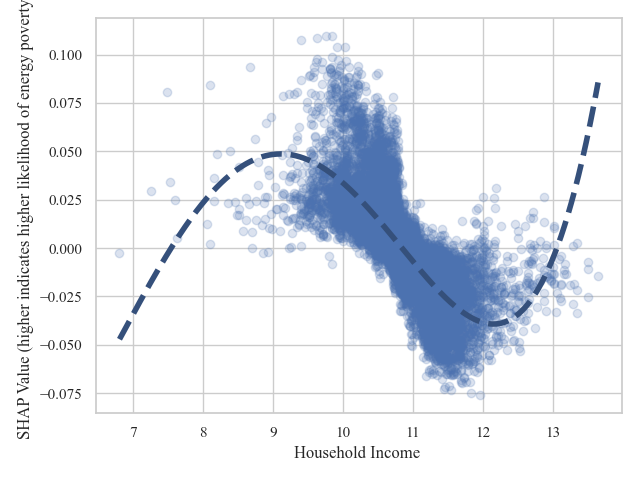
\includegraphics[width=\textwidth]{Figure4a.png}
     \end{subfigure}
     \hfill
     \begin{subfigure}[b]{0.45\textwidth}
         \centering
         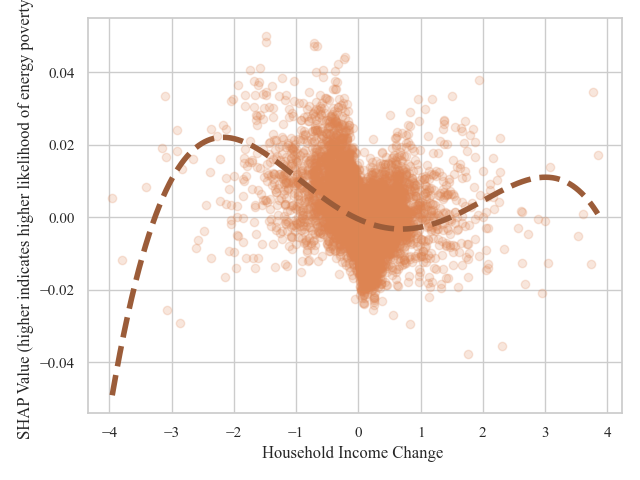
\includegraphics[width=\textwidth]{Figure4b.png}
     \end{subfigure}
     \hfill
     \begin{subfigure}[b]{0.45\textwidth}
         \centering
         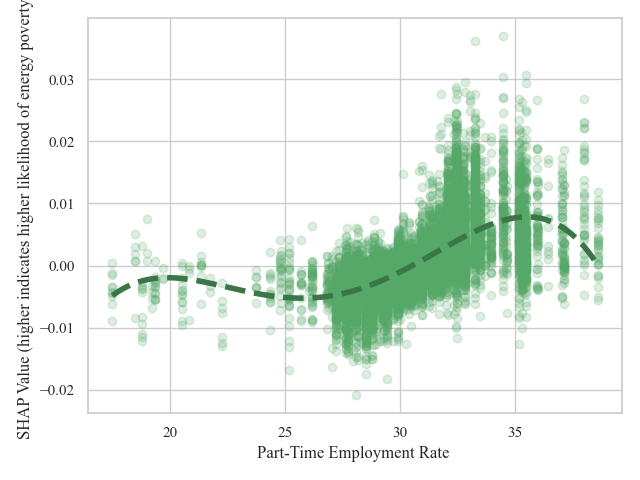
\includegraphics[width=\textwidth]{Figure4c.png}
     \end{subfigure}
     \hfill
     \begin{subfigure}[b]{0.45\textwidth}
         \centering
         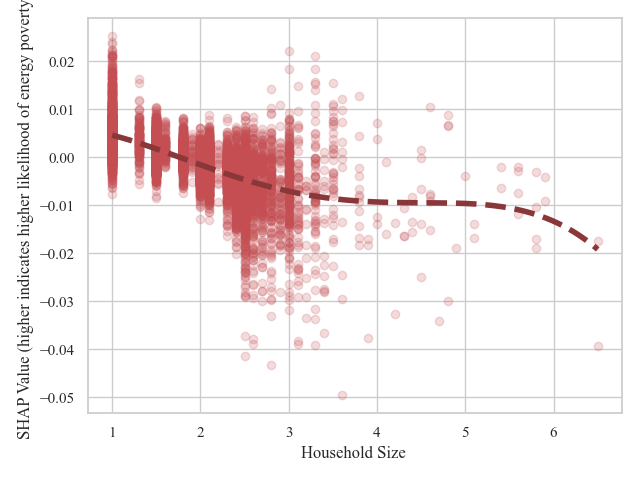
\includegraphics[width=\textwidth]{Figure4d.png}
     \end{subfigure}
     \hfill
     \begin{subfigure}[b]{0.45\textwidth}
         \centering
         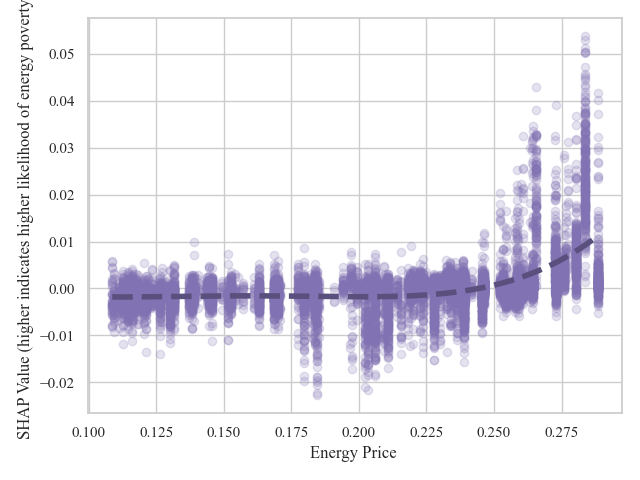
\includegraphics[width=\textwidth]{Figure4e.png}
     \end{subfigure}
     \caption{Relationship between key predictive variables and \Gls{shap} values for energy poverty outcomes. \\
    \small
    {\bf Notes:} i) Each point represents a household, with the x-axis indicating the feature value and the y-axis showing the \Gls{shap} value, which reflects the feature's contribution to the forecasting. Positive \Gls{shap} values indicate a higher likelihood of energy poverty, while negative values suggest a reduced risk. The plots highlight how changes in the variables influence the model's forecasts; ii) The dashed lines summarize the underlying trends and were calculated using a least squares polynomial fit of degree 4. The interpolations at the extremes of the plots may lack reliability due to the sparse data points in these regions, potentially leading to less accurate representations of the trend; iii) Source: \Gls{hilda} 2007--2021 waves.}
    \label{fig:figure4}
\end{figure}


The part-time employment rate contributes to the energy poverty risk, particularly in areas where the part-time employment rate exceeds 30\%. One possible explanation is that part-time jobs reflect labor market and income instability. These positions often lack critical benefits, such as health insurance or retirement plans, which heightens financial vulnerability. Additionally, fluctuating hours and earnings further amplify economic uncertainty. At lower part-time employment rates (below 25\%), \Gls{shap} values remain relatively stable, indicating a minimal influence. These findings indicate that policies promoting income stability, benefits for part-time workers, and access to full-time employment opportunities are crucial for tackling energy poverty in regions with high part-time employment rates. Additionally, the results in \Cref{fig:figure3} reveal that regional labor market dynamics can have delayed impacts on energy poverty, suggesting that such policies could produce lasting effects. 

The relationship between household size and \Gls{shap} values highlights a clear risk group: people living alone or in two-person households. This is likely because fixed energy costs pose a disproportionately heavy burden on them. As household size increases to 3--4 members, the likelihood of energy poverty decreases, likely reflecting economies of scale in energy consumption, which reduce the per-capita cost burden.

Lastly, energy prices display a notable pattern, suggesting that below a certain threshold, they are not relevant for energy poverty. At low price levels, \Gls{shap} values remain relatively stable, but they increase steadily above \$0.228 and rise significantly beyond \$0.266. This is a relevant finding, as most representations in the literature describe the effect of energy prices on energy poverty in a linear, average manner. However, the results indicate that the relationship between energy prices and energy poverty is non-linear and nearly flat within certain ranges. In this context, energy subsidies and price controls may be ineffective within these ranges, whereas informational campaigns and targeted support for individuals exposed to high prices could play a crucial role. 

%%%%%%%%%%%%%%%%%%%%%%%%%%%%%%%%%%%%%%%%%%%%%%%%%%%%%%%%%%%%%%%%%%%%%

%%%%%%%%%%%%%%%%%%%%%%%%%%%%%%%%%%%%%%%%%%%%%%%%%%%%%%%%%%%%%%%%%%%%%
%%%%%%%%%%%%%%%%%%%%%%%%%%%%%%%%%%%%%%%%%%%%%%%%%%%%%%%%%%%%%%%%%%%%%
%%%%%%%%%%%%%%%%%%%%%%%%%%%%%%%%%%%%%%%%%%%%%%%%%%%%%%%%%%%%%%%%%%%%%
\section{Sensitivity checks} \label{Sensitivity_checks}
%%%%%%%%%%%%%%%%%%%%%%%%%%%%%%%%%%%%%%%%%%%%%%%%%%%%%%%%%%%%%%%%%%%%%
%%%%%%%%%%%%%%%%%%%%%%%%%%%%%%%%%%%%%%%%%%%%%%%%%%%%%%%%%%%%%%%%%%%%%
%%%%%%%%%%%%%%%%%%%%%%%%%%%%%%%%%%%%%%%%%%%%%%%%%%%%%%%%%%%%%%%%%%%%%

In this section, we conduct a series of supplementary analyses. Specifically, we explore the sensitivity of the results to variations in i) the time length considered for the analysis and ii) the chosen cut-off point for defining the energy poverty line. We also examine to what extent our findings might be affected by selection and attrition bias. 

In \Cref{fig:figure5} we depict the relative contribution of the predictive variables for alternative time spans. The results show robust consistency across scenarios, with household income emerging as the most significant determinant of energy poverty, irrespective of the time span. Notably, the predictive power of income changes significantly, increasing more than threefold from about 5\% when $T=2$ to over 17\% when $T=12$ or $T=14$. This suggests that income volatility and the uncertainty it creates are crucial factors influencing long-term energy poverty outcomes. 

Additionally, energy prices are relatively important in the short term (6--7\%), but their relevance decreases over the long-term ($<4$\%). Similarly, improvements in education levels are more strongly associated with short-term energy poverty outcomes than with long-term ones. Household size maintains a consistent level of importance across both short- and long-term periods, reinforcing its stable role as a determinant of energy poverty. 

%%%%%%%%%%%%%%%%%%%%%%%%%%%%%%%%%%%%%%%%%%%%%%%%%%%%%%%%%%%%%%%%%%%%%
\begin{figure}
     \centering
     \begin{subfigure}[b]{0.45\textwidth}
         \centering
         \resizebox{\textwidth}{!}{%% Creator: Matplotlib, PGF backend
%%
%% To include the figure in your LaTeX document, write
%%   \input{<filename>.pgf}
%%
%% Make sure the required packages are loaded in your preamble
%%   \usepackage{pgf}
%%
%% Also ensure that all the required font packages are loaded; for instance,
%% the lmodern package is sometimes necessary when using math font.
%%   \usepackage{lmodern}
%%
%% Figures using additional raster images can only be included by \input if
%% they are in the same directory as the main LaTeX file. For loading figures
%% from other directories you can use the `import` package
%%   \usepackage{import}
%%
%% and then include the figures with
%%   \import{<path to file>}{<filename>.pgf}
%%
%% Matplotlib used the following preamble
%%   
%%   \makeatletter\@ifpackageloaded{underscore}{}{\usepackage[strings]{underscore}}\makeatother
%%
\begingroup%
\makeatletter%
\begin{pgfpicture}%
\pgfpathrectangle{\pgfpointorigin}{\pgfqpoint{6.400000in}{4.800000in}}%
\pgfusepath{use as bounding box, clip}%
\begin{pgfscope}%
\pgfsetbuttcap%
\pgfsetmiterjoin%
\definecolor{currentfill}{rgb}{1.000000,1.000000,1.000000}%
\pgfsetfillcolor{currentfill}%
\pgfsetlinewidth{0.000000pt}%
\definecolor{currentstroke}{rgb}{1.000000,1.000000,1.000000}%
\pgfsetstrokecolor{currentstroke}%
\pgfsetdash{}{0pt}%
\pgfpathmoveto{\pgfqpoint{0.000000in}{0.000000in}}%
\pgfpathlineto{\pgfqpoint{6.400000in}{0.000000in}}%
\pgfpathlineto{\pgfqpoint{6.400000in}{4.800000in}}%
\pgfpathlineto{\pgfqpoint{0.000000in}{4.800000in}}%
\pgfpathlineto{\pgfqpoint{0.000000in}{0.000000in}}%
\pgfpathclose%
\pgfusepath{fill}%
\end{pgfscope}%
\begin{pgfscope}%
\pgfsetbuttcap%
\pgfsetmiterjoin%
\definecolor{currentfill}{rgb}{1.000000,1.000000,1.000000}%
\pgfsetfillcolor{currentfill}%
\pgfsetlinewidth{0.000000pt}%
\definecolor{currentstroke}{rgb}{0.000000,0.000000,0.000000}%
\pgfsetstrokecolor{currentstroke}%
\pgfsetstrokeopacity{0.000000}%
\pgfsetdash{}{0pt}%
\pgfpathmoveto{\pgfqpoint{3.055864in}{0.669352in}}%
\pgfpathlineto{\pgfqpoint{5.870703in}{0.669352in}}%
\pgfpathlineto{\pgfqpoint{5.870703in}{4.620000in}}%
\pgfpathlineto{\pgfqpoint{3.055864in}{4.620000in}}%
\pgfpathlineto{\pgfqpoint{3.055864in}{0.669352in}}%
\pgfpathclose%
\pgfusepath{fill}%
\end{pgfscope}%
\begin{pgfscope}%
\pgfpathrectangle{\pgfqpoint{3.055864in}{0.669352in}}{\pgfqpoint{2.814839in}{3.950648in}}%
\pgfusepath{clip}%
\pgfsetroundcap%
\pgfsetroundjoin%
\pgfsetlinewidth{1.003750pt}%
\definecolor{currentstroke}{rgb}{0.800000,0.800000,0.800000}%
\pgfsetstrokecolor{currentstroke}%
\pgfsetdash{}{0pt}%
\pgfpathmoveto{\pgfqpoint{3.055864in}{0.669352in}}%
\pgfpathlineto{\pgfqpoint{3.055864in}{4.620000in}}%
\pgfusepath{stroke}%
\end{pgfscope}%
\begin{pgfscope}%
\definecolor{textcolor}{rgb}{0.150000,0.150000,0.150000}%
\pgfsetstrokecolor{textcolor}%
\pgfsetfillcolor{textcolor}%
\pgftext[x=3.055864in,y=0.537407in,,top]{\color{textcolor}\fontsize{11.000000}{13.200000}\selectfont \(\displaystyle {0}\)}%
\end{pgfscope}%
\begin{pgfscope}%
\pgfpathrectangle{\pgfqpoint{3.055864in}{0.669352in}}{\pgfqpoint{2.814839in}{3.950648in}}%
\pgfusepath{clip}%
\pgfsetroundcap%
\pgfsetroundjoin%
\pgfsetlinewidth{1.003750pt}%
\definecolor{currentstroke}{rgb}{0.800000,0.800000,0.800000}%
\pgfsetstrokecolor{currentstroke}%
\pgfsetdash{}{0pt}%
\pgfpathmoveto{\pgfqpoint{3.938645in}{0.669352in}}%
\pgfpathlineto{\pgfqpoint{3.938645in}{4.620000in}}%
\pgfusepath{stroke}%
\end{pgfscope}%
\begin{pgfscope}%
\definecolor{textcolor}{rgb}{0.150000,0.150000,0.150000}%
\pgfsetstrokecolor{textcolor}%
\pgfsetfillcolor{textcolor}%
\pgftext[x=3.938645in,y=0.537407in,,top]{\color{textcolor}\fontsize{11.000000}{13.200000}\selectfont \(\displaystyle {10}\)}%
\end{pgfscope}%
\begin{pgfscope}%
\pgfpathrectangle{\pgfqpoint{3.055864in}{0.669352in}}{\pgfqpoint{2.814839in}{3.950648in}}%
\pgfusepath{clip}%
\pgfsetroundcap%
\pgfsetroundjoin%
\pgfsetlinewidth{1.003750pt}%
\definecolor{currentstroke}{rgb}{0.800000,0.800000,0.800000}%
\pgfsetstrokecolor{currentstroke}%
\pgfsetdash{}{0pt}%
\pgfpathmoveto{\pgfqpoint{4.821426in}{0.669352in}}%
\pgfpathlineto{\pgfqpoint{4.821426in}{4.620000in}}%
\pgfusepath{stroke}%
\end{pgfscope}%
\begin{pgfscope}%
\definecolor{textcolor}{rgb}{0.150000,0.150000,0.150000}%
\pgfsetstrokecolor{textcolor}%
\pgfsetfillcolor{textcolor}%
\pgftext[x=4.821426in,y=0.537407in,,top]{\color{textcolor}\fontsize{11.000000}{13.200000}\selectfont \(\displaystyle {20}\)}%
\end{pgfscope}%
\begin{pgfscope}%
\pgfpathrectangle{\pgfqpoint{3.055864in}{0.669352in}}{\pgfqpoint{2.814839in}{3.950648in}}%
\pgfusepath{clip}%
\pgfsetroundcap%
\pgfsetroundjoin%
\pgfsetlinewidth{1.003750pt}%
\definecolor{currentstroke}{rgb}{0.800000,0.800000,0.800000}%
\pgfsetstrokecolor{currentstroke}%
\pgfsetdash{}{0pt}%
\pgfpathmoveto{\pgfqpoint{5.704207in}{0.669352in}}%
\pgfpathlineto{\pgfqpoint{5.704207in}{4.620000in}}%
\pgfusepath{stroke}%
\end{pgfscope}%
\begin{pgfscope}%
\definecolor{textcolor}{rgb}{0.150000,0.150000,0.150000}%
\pgfsetstrokecolor{textcolor}%
\pgfsetfillcolor{textcolor}%
\pgftext[x=5.704207in,y=0.537407in,,top]{\color{textcolor}\fontsize{11.000000}{13.200000}\selectfont \(\displaystyle {30}\)}%
\end{pgfscope}%
\begin{pgfscope}%
\definecolor{textcolor}{rgb}{0.150000,0.150000,0.150000}%
\pgfsetstrokecolor{textcolor}%
\pgfsetfillcolor{textcolor}%
\pgftext[x=4.463283in,y=0.346667in,,top]{\color{textcolor}\fontsize{12.000000}{14.400000}\selectfont Summed Normalized Importance (\%)}%
\end{pgfscope}%
\begin{pgfscope}%
\definecolor{textcolor}{rgb}{0.150000,0.150000,0.150000}%
\pgfsetstrokecolor{textcolor}%
\pgfsetfillcolor{textcolor}%
\pgftext[x=1.655712in, y=4.435505in, left, base]{\color{textcolor}\fontsize{11.000000}{13.200000}\selectfont Household Income }%
\end{pgfscope}%
\begin{pgfscope}%
\definecolor{textcolor}{rgb}{0.150000,0.150000,0.150000}%
\pgfsetstrokecolor{textcolor}%
\pgfsetfillcolor{textcolor}%
\pgftext[x=1.606708in, y=4.172129in, left, base]{\color{textcolor}\fontsize{11.000000}{13.200000}\selectfont Years of Education }%
\end{pgfscope}%
\begin{pgfscope}%
\definecolor{textcolor}{rgb}{0.150000,0.150000,0.150000}%
\pgfsetstrokecolor{textcolor}%
\pgfsetfillcolor{textcolor}%
\pgftext[x=1.556435in, y=3.908752in, left, base]{\color{textcolor}\fontsize{11.000000}{13.200000}\selectfont Employment Status }%
\end{pgfscope}%
\begin{pgfscope}%
\definecolor{textcolor}{rgb}{0.150000,0.150000,0.150000}%
\pgfsetstrokecolor{textcolor}%
\pgfsetfillcolor{textcolor}%
\pgftext[x=2.010573in, y=3.645375in, left, base]{\color{textcolor}\fontsize{11.000000}{13.200000}\selectfont Energy Price }%
\end{pgfscope}%
\begin{pgfscope}%
\definecolor{textcolor}{rgb}{0.150000,0.150000,0.150000}%
\pgfsetstrokecolor{textcolor}%
\pgfsetfillcolor{textcolor}%
\pgftext[x=0.923177in, y=3.381999in, left, base]{\color{textcolor}\fontsize{11.000000}{13.200000}\selectfont Part-Time Employment Rate }%
\end{pgfscope}%
\begin{pgfscope}%
\definecolor{textcolor}{rgb}{0.150000,0.150000,0.150000}%
\pgfsetstrokecolor{textcolor}%
\pgfsetfillcolor{textcolor}%
\pgftext[x=1.871164in, y=3.118622in, left, base]{\color{textcolor}\fontsize{11.000000}{13.200000}\selectfont Household Size }%
\end{pgfscope}%
\begin{pgfscope}%
\definecolor{textcolor}{rgb}{0.150000,0.150000,0.150000}%
\pgfsetstrokecolor{textcolor}%
\pgfsetfillcolor{textcolor}%
\pgftext[x=0.743634in, y=2.855246in, left, base]{\color{textcolor}\fontsize{11.000000}{13.200000}\selectfont Children Presence at Household }%
\end{pgfscope}%
\begin{pgfscope}%
\definecolor{textcolor}{rgb}{0.150000,0.150000,0.150000}%
\pgfsetstrokecolor{textcolor}%
\pgfsetfillcolor{textcolor}%
\pgftext[x=1.106522in, y=2.591869in, left, base]{\color{textcolor}\fontsize{11.000000}{13.200000}\selectfont Household Income Change }%
\end{pgfscope}%
\begin{pgfscope}%
\definecolor{textcolor}{rgb}{0.150000,0.150000,0.150000}%
\pgfsetstrokecolor{textcolor}%
\pgfsetfillcolor{textcolor}%
\pgftext[x=2.063803in, y=2.328493in, left, base]{\color{textcolor}\fontsize{11.000000}{13.200000}\selectfont Poor Health }%
\end{pgfscope}%
\begin{pgfscope}%
\definecolor{textcolor}{rgb}{0.150000,0.150000,0.150000}%
\pgfsetstrokecolor{textcolor}%
\pgfsetfillcolor{textcolor}%
\pgftext[x=1.870318in, y=2.065116in, left, base]{\color{textcolor}\fontsize{11.000000}{13.200000}\selectfont Married Status }%
\end{pgfscope}%
\begin{pgfscope}%
\definecolor{textcolor}{rgb}{0.150000,0.150000,0.150000}%
\pgfsetstrokecolor{textcolor}%
\pgfsetfillcolor{textcolor}%
\pgftext[x=1.790264in, y=1.801740in, left, base]{\color{textcolor}\fontsize{11.000000}{13.200000}\selectfont GSP Per Capita }%
\end{pgfscope}%
\begin{pgfscope}%
\definecolor{textcolor}{rgb}{0.150000,0.150000,0.150000}%
\pgfsetstrokecolor{textcolor}%
\pgfsetfillcolor{textcolor}%
\pgftext[x=1.235370in, y=1.538363in, left, base]{\color{textcolor}\fontsize{11.000000}{13.200000}\selectfont GSP Per Capita Growth }%
\end{pgfscope}%
\begin{pgfscope}%
\definecolor{textcolor}{rgb}{0.150000,0.150000,0.150000}%
\pgfsetstrokecolor{textcolor}%
\pgfsetfillcolor{textcolor}%
\pgftext[x=0.383703in, y=1.274987in, left, base]{\color{textcolor}\fontsize{11.000000}{13.200000}\selectfont Total Labor Force Participation Rate }%
\end{pgfscope}%
\begin{pgfscope}%
\definecolor{textcolor}{rgb}{0.150000,0.150000,0.150000}%
\pgfsetstrokecolor{textcolor}%
\pgfsetfillcolor{textcolor}%
\pgftext[x=1.502361in, y=1.011610in, left, base]{\color{textcolor}\fontsize{11.000000}{13.200000}\selectfont Unemployment Rate }%
\end{pgfscope}%
\begin{pgfscope}%
\definecolor{textcolor}{rgb}{0.150000,0.150000,0.150000}%
\pgfsetstrokecolor{textcolor}%
\pgfsetfillcolor{textcolor}%
\pgftext[x=1.809485in, y=0.748233in, left, base]{\color{textcolor}\fontsize{11.000000}{13.200000}\selectfont Divorced Status }%
\end{pgfscope}%
\begin{pgfscope}%
\definecolor{textcolor}{rgb}{0.150000,0.150000,0.150000}%
\pgfsetstrokecolor{textcolor}%
\pgfsetfillcolor{textcolor}%
\pgftext[x=0.328147in,y=2.644676in,,bottom,rotate=90.000000]{\color{textcolor}\fontsize{12.000000}{14.400000}\selectfont Variable}%
\end{pgfscope}%
\begin{pgfscope}%
\pgfpathrectangle{\pgfqpoint{3.055864in}{0.669352in}}{\pgfqpoint{2.814839in}{3.950648in}}%
\pgfusepath{clip}%
\pgfsetbuttcap%
\pgfsetmiterjoin%
\definecolor{currentfill}{rgb}{0.718772,0.299398,0.288032}%
\pgfsetfillcolor{currentfill}%
\pgfsetlinewidth{1.003750pt}%
\definecolor{currentstroke}{rgb}{1.000000,1.000000,1.000000}%
\pgfsetstrokecolor{currentstroke}%
\pgfsetdash{}{0pt}%
\pgfpathmoveto{\pgfqpoint{3.055864in}{4.593662in}}%
\pgfpathlineto{\pgfqpoint{5.736663in}{4.593662in}}%
\pgfpathlineto{\pgfqpoint{5.736663in}{4.382961in}}%
\pgfpathlineto{\pgfqpoint{3.055864in}{4.382961in}}%
\pgfpathlineto{\pgfqpoint{3.055864in}{4.593662in}}%
\pgfpathclose%
\pgfusepath{stroke,fill}%
\end{pgfscope}%
\begin{pgfscope}%
\pgfpathrectangle{\pgfqpoint{3.055864in}{0.669352in}}{\pgfqpoint{2.814839in}{3.950648in}}%
\pgfusepath{clip}%
\pgfsetbuttcap%
\pgfsetmiterjoin%
\definecolor{currentfill}{rgb}{0.794189,0.423491,0.366972}%
\pgfsetfillcolor{currentfill}%
\pgfsetlinewidth{1.003750pt}%
\definecolor{currentstroke}{rgb}{1.000000,1.000000,1.000000}%
\pgfsetstrokecolor{currentstroke}%
\pgfsetdash{}{0pt}%
\pgfpathmoveto{\pgfqpoint{3.055864in}{4.330286in}}%
\pgfpathlineto{\pgfqpoint{4.065580in}{4.330286in}}%
\pgfpathlineto{\pgfqpoint{4.065580in}{4.119585in}}%
\pgfpathlineto{\pgfqpoint{3.055864in}{4.119585in}}%
\pgfpathlineto{\pgfqpoint{3.055864in}{4.330286in}}%
\pgfpathclose%
\pgfusepath{stroke,fill}%
\end{pgfscope}%
\begin{pgfscope}%
\pgfpathrectangle{\pgfqpoint{3.055864in}{0.669352in}}{\pgfqpoint{2.814839in}{3.950648in}}%
\pgfusepath{clip}%
\pgfsetbuttcap%
\pgfsetmiterjoin%
\definecolor{currentfill}{rgb}{0.854156,0.531667,0.450658}%
\pgfsetfillcolor{currentfill}%
\pgfsetlinewidth{1.003750pt}%
\definecolor{currentstroke}{rgb}{1.000000,1.000000,1.000000}%
\pgfsetstrokecolor{currentstroke}%
\pgfsetdash{}{0pt}%
\pgfpathmoveto{\pgfqpoint{3.055864in}{4.066909in}}%
\pgfpathlineto{\pgfqpoint{3.682161in}{4.066909in}}%
\pgfpathlineto{\pgfqpoint{3.682161in}{3.856208in}}%
\pgfpathlineto{\pgfqpoint{3.055864in}{3.856208in}}%
\pgfpathlineto{\pgfqpoint{3.055864in}{4.066909in}}%
\pgfpathclose%
\pgfusepath{stroke,fill}%
\end{pgfscope}%
\begin{pgfscope}%
\pgfpathrectangle{\pgfqpoint{3.055864in}{0.669352in}}{\pgfqpoint{2.814839in}{3.950648in}}%
\pgfusepath{clip}%
\pgfsetbuttcap%
\pgfsetmiterjoin%
\definecolor{currentfill}{rgb}{0.896734,0.627770,0.537221}%
\pgfsetfillcolor{currentfill}%
\pgfsetlinewidth{1.003750pt}%
\definecolor{currentstroke}{rgb}{1.000000,1.000000,1.000000}%
\pgfsetstrokecolor{currentstroke}%
\pgfsetdash{}{0pt}%
\pgfpathmoveto{\pgfqpoint{3.055864in}{3.803533in}}%
\pgfpathlineto{\pgfqpoint{3.681491in}{3.803533in}}%
\pgfpathlineto{\pgfqpoint{3.681491in}{3.592831in}}%
\pgfpathlineto{\pgfqpoint{3.055864in}{3.592831in}}%
\pgfpathlineto{\pgfqpoint{3.055864in}{3.803533in}}%
\pgfpathclose%
\pgfusepath{stroke,fill}%
\end{pgfscope}%
\begin{pgfscope}%
\pgfpathrectangle{\pgfqpoint{3.055864in}{0.669352in}}{\pgfqpoint{2.814839in}{3.950648in}}%
\pgfusepath{clip}%
\pgfsetbuttcap%
\pgfsetmiterjoin%
\definecolor{currentfill}{rgb}{0.920365,0.710966,0.624456}%
\pgfsetfillcolor{currentfill}%
\pgfsetlinewidth{1.003750pt}%
\definecolor{currentstroke}{rgb}{1.000000,1.000000,1.000000}%
\pgfsetstrokecolor{currentstroke}%
\pgfsetdash{}{0pt}%
\pgfpathmoveto{\pgfqpoint{3.055864in}{3.540156in}}%
\pgfpathlineto{\pgfqpoint{3.587197in}{3.540156in}}%
\pgfpathlineto{\pgfqpoint{3.587197in}{3.329455in}}%
\pgfpathlineto{\pgfqpoint{3.055864in}{3.329455in}}%
\pgfpathlineto{\pgfqpoint{3.055864in}{3.540156in}}%
\pgfpathclose%
\pgfusepath{stroke,fill}%
\end{pgfscope}%
\begin{pgfscope}%
\pgfpathrectangle{\pgfqpoint{3.055864in}{0.669352in}}{\pgfqpoint{2.814839in}{3.950648in}}%
\pgfusepath{clip}%
\pgfsetbuttcap%
\pgfsetmiterjoin%
\definecolor{currentfill}{rgb}{0.923846,0.779437,0.709816}%
\pgfsetfillcolor{currentfill}%
\pgfsetlinewidth{1.003750pt}%
\definecolor{currentstroke}{rgb}{1.000000,1.000000,1.000000}%
\pgfsetstrokecolor{currentstroke}%
\pgfsetdash{}{0pt}%
\pgfpathmoveto{\pgfqpoint{3.055864in}{3.276780in}}%
\pgfpathlineto{\pgfqpoint{3.570751in}{3.276780in}}%
\pgfpathlineto{\pgfqpoint{3.570751in}{3.066078in}}%
\pgfpathlineto{\pgfqpoint{3.055864in}{3.066078in}}%
\pgfpathlineto{\pgfqpoint{3.055864in}{3.276780in}}%
\pgfpathclose%
\pgfusepath{stroke,fill}%
\end{pgfscope}%
\begin{pgfscope}%
\pgfpathrectangle{\pgfqpoint{3.055864in}{0.669352in}}{\pgfqpoint{2.814839in}{3.950648in}}%
\pgfusepath{clip}%
\pgfsetbuttcap%
\pgfsetmiterjoin%
\definecolor{currentfill}{rgb}{0.906260,0.831225,0.790440}%
\pgfsetfillcolor{currentfill}%
\pgfsetlinewidth{1.003750pt}%
\definecolor{currentstroke}{rgb}{1.000000,1.000000,1.000000}%
\pgfsetstrokecolor{currentstroke}%
\pgfsetdash{}{0pt}%
\pgfpathmoveto{\pgfqpoint{3.055864in}{3.013403in}}%
\pgfpathlineto{\pgfqpoint{3.565439in}{3.013403in}}%
\pgfpathlineto{\pgfqpoint{3.565439in}{2.802702in}}%
\pgfpathlineto{\pgfqpoint{3.055864in}{2.802702in}}%
\pgfpathlineto{\pgfqpoint{3.055864in}{3.013403in}}%
\pgfpathclose%
\pgfusepath{stroke,fill}%
\end{pgfscope}%
\begin{pgfscope}%
\pgfpathrectangle{\pgfqpoint{3.055864in}{0.669352in}}{\pgfqpoint{2.814839in}{3.950648in}}%
\pgfusepath{clip}%
\pgfsetbuttcap%
\pgfsetmiterjoin%
\definecolor{currentfill}{rgb}{0.866824,0.864536,0.863206}%
\pgfsetfillcolor{currentfill}%
\pgfsetlinewidth{1.003750pt}%
\definecolor{currentstroke}{rgb}{1.000000,1.000000,1.000000}%
\pgfsetstrokecolor{currentstroke}%
\pgfsetdash{}{0pt}%
\pgfpathmoveto{\pgfqpoint{3.055864in}{2.750027in}}%
\pgfpathlineto{\pgfqpoint{3.516840in}{2.750027in}}%
\pgfpathlineto{\pgfqpoint{3.516840in}{2.539325in}}%
\pgfpathlineto{\pgfqpoint{3.055864in}{2.539325in}}%
\pgfpathlineto{\pgfqpoint{3.055864in}{2.750027in}}%
\pgfpathclose%
\pgfusepath{stroke,fill}%
\end{pgfscope}%
\begin{pgfscope}%
\pgfpathrectangle{\pgfqpoint{3.055864in}{0.669352in}}{\pgfqpoint{2.814839in}{3.950648in}}%
\pgfusepath{clip}%
\pgfsetbuttcap%
\pgfsetmiterjoin%
\definecolor{currentfill}{rgb}{0.816777,0.854095,0.913832}%
\pgfsetfillcolor{currentfill}%
\pgfsetlinewidth{1.003750pt}%
\definecolor{currentstroke}{rgb}{1.000000,1.000000,1.000000}%
\pgfsetstrokecolor{currentstroke}%
\pgfsetdash{}{0pt}%
\pgfpathmoveto{\pgfqpoint{3.055864in}{2.486650in}}%
\pgfpathlineto{\pgfqpoint{3.471564in}{2.486650in}}%
\pgfpathlineto{\pgfqpoint{3.471564in}{2.275949in}}%
\pgfpathlineto{\pgfqpoint{3.055864in}{2.275949in}}%
\pgfpathlineto{\pgfqpoint{3.055864in}{2.486650in}}%
\pgfpathclose%
\pgfusepath{stroke,fill}%
\end{pgfscope}%
\begin{pgfscope}%
\pgfpathrectangle{\pgfqpoint{3.055864in}{0.669352in}}{\pgfqpoint{2.814839in}{3.950648in}}%
\pgfusepath{clip}%
\pgfsetbuttcap%
\pgfsetmiterjoin%
\definecolor{currentfill}{rgb}{0.755493,0.823644,0.944200}%
\pgfsetfillcolor{currentfill}%
\pgfsetlinewidth{1.003750pt}%
\definecolor{currentstroke}{rgb}{1.000000,1.000000,1.000000}%
\pgfsetstrokecolor{currentstroke}%
\pgfsetdash{}{0pt}%
\pgfpathmoveto{\pgfqpoint{3.055864in}{2.223273in}}%
\pgfpathlineto{\pgfqpoint{3.370949in}{2.223273in}}%
\pgfpathlineto{\pgfqpoint{3.370949in}{2.012572in}}%
\pgfpathlineto{\pgfqpoint{3.055864in}{2.012572in}}%
\pgfpathlineto{\pgfqpoint{3.055864in}{2.223273in}}%
\pgfpathclose%
\pgfusepath{stroke,fill}%
\end{pgfscope}%
\begin{pgfscope}%
\pgfpathrectangle{\pgfqpoint{3.055864in}{0.669352in}}{\pgfqpoint{2.814839in}{3.950648in}}%
\pgfusepath{clip}%
\pgfsetbuttcap%
\pgfsetmiterjoin%
\definecolor{currentfill}{rgb}{0.685455,0.775398,0.953219}%
\pgfsetfillcolor{currentfill}%
\pgfsetlinewidth{1.003750pt}%
\definecolor{currentstroke}{rgb}{1.000000,1.000000,1.000000}%
\pgfsetstrokecolor{currentstroke}%
\pgfsetdash{}{0pt}%
\pgfpathmoveto{\pgfqpoint{3.055864in}{1.959897in}}%
\pgfpathlineto{\pgfqpoint{3.233809in}{1.959897in}}%
\pgfpathlineto{\pgfqpoint{3.233809in}{1.749196in}}%
\pgfpathlineto{\pgfqpoint{3.055864in}{1.749196in}}%
\pgfpathlineto{\pgfqpoint{3.055864in}{1.959897in}}%
\pgfpathclose%
\pgfusepath{stroke,fill}%
\end{pgfscope}%
\begin{pgfscope}%
\pgfpathrectangle{\pgfqpoint{3.055864in}{0.669352in}}{\pgfqpoint{2.814839in}{3.950648in}}%
\pgfusepath{clip}%
\pgfsetbuttcap%
\pgfsetmiterjoin%
\definecolor{currentfill}{rgb}{0.609462,0.711301,0.940365}%
\pgfsetfillcolor{currentfill}%
\pgfsetlinewidth{1.003750pt}%
\definecolor{currentstroke}{rgb}{1.000000,1.000000,1.000000}%
\pgfsetstrokecolor{currentstroke}%
\pgfsetdash{}{0pt}%
\pgfpathmoveto{\pgfqpoint{3.055864in}{1.696520in}}%
\pgfpathlineto{\pgfqpoint{3.230410in}{1.696520in}}%
\pgfpathlineto{\pgfqpoint{3.230410in}{1.485819in}}%
\pgfpathlineto{\pgfqpoint{3.055864in}{1.485819in}}%
\pgfpathlineto{\pgfqpoint{3.055864in}{1.696520in}}%
\pgfpathclose%
\pgfusepath{stroke,fill}%
\end{pgfscope}%
\begin{pgfscope}%
\pgfpathrectangle{\pgfqpoint{3.055864in}{0.669352in}}{\pgfqpoint{2.814839in}{3.950648in}}%
\pgfusepath{clip}%
\pgfsetbuttcap%
\pgfsetmiterjoin%
\definecolor{currentfill}{rgb}{0.530287,0.633721,0.905938}%
\pgfsetfillcolor{currentfill}%
\pgfsetlinewidth{1.003750pt}%
\definecolor{currentstroke}{rgb}{1.000000,1.000000,1.000000}%
\pgfsetstrokecolor{currentstroke}%
\pgfsetdash{}{0pt}%
\pgfpathmoveto{\pgfqpoint{3.055864in}{1.433144in}}%
\pgfpathlineto{\pgfqpoint{3.228667in}{1.433144in}}%
\pgfpathlineto{\pgfqpoint{3.228667in}{1.222443in}}%
\pgfpathlineto{\pgfqpoint{3.055864in}{1.222443in}}%
\pgfpathlineto{\pgfqpoint{3.055864in}{1.433144in}}%
\pgfpathclose%
\pgfusepath{stroke,fill}%
\end{pgfscope}%
\begin{pgfscope}%
\pgfpathrectangle{\pgfqpoint{3.055864in}{0.669352in}}{\pgfqpoint{2.814839in}{3.950648in}}%
\pgfusepath{clip}%
\pgfsetbuttcap%
\pgfsetmiterjoin%
\definecolor{currentfill}{rgb}{0.450433,0.545324,0.851060}%
\pgfsetfillcolor{currentfill}%
\pgfsetlinewidth{1.003750pt}%
\definecolor{currentstroke}{rgb}{1.000000,1.000000,1.000000}%
\pgfsetstrokecolor{currentstroke}%
\pgfsetdash{}{0pt}%
\pgfpathmoveto{\pgfqpoint{3.055864in}{1.169767in}}%
\pgfpathlineto{\pgfqpoint{3.207047in}{1.169767in}}%
\pgfpathlineto{\pgfqpoint{3.207047in}{0.959066in}}%
\pgfpathlineto{\pgfqpoint{3.055864in}{0.959066in}}%
\pgfpathlineto{\pgfqpoint{3.055864in}{1.169767in}}%
\pgfpathclose%
\pgfusepath{stroke,fill}%
\end{pgfscope}%
\begin{pgfscope}%
\pgfpathrectangle{\pgfqpoint{3.055864in}{0.669352in}}{\pgfqpoint{2.814839in}{3.950648in}}%
\pgfusepath{clip}%
\pgfsetbuttcap%
\pgfsetmiterjoin%
\definecolor{currentfill}{rgb}{0.371810,0.448888,0.777627}%
\pgfsetfillcolor{currentfill}%
\pgfsetlinewidth{1.003750pt}%
\definecolor{currentstroke}{rgb}{1.000000,1.000000,1.000000}%
\pgfsetstrokecolor{currentstroke}%
\pgfsetdash{}{0pt}%
\pgfpathmoveto{\pgfqpoint{3.055864in}{0.906391in}}%
\pgfpathlineto{\pgfqpoint{3.197930in}{0.906391in}}%
\pgfpathlineto{\pgfqpoint{3.197930in}{0.695689in}}%
\pgfpathlineto{\pgfqpoint{3.055864in}{0.695689in}}%
\pgfpathlineto{\pgfqpoint{3.055864in}{0.906391in}}%
\pgfpathclose%
\pgfusepath{stroke,fill}%
\end{pgfscope}%
\begin{pgfscope}%
\pgfpathrectangle{\pgfqpoint{3.055864in}{0.669352in}}{\pgfqpoint{2.814839in}{3.950648in}}%
\pgfusepath{clip}%
\pgfsetroundcap%
\pgfsetroundjoin%
\pgfsetlinewidth{2.258437pt}%
\definecolor{currentstroke}{rgb}{0.260000,0.260000,0.260000}%
\pgfsetstrokecolor{currentstroke}%
\pgfsetdash{}{0pt}%
\pgfusepath{stroke}%
\end{pgfscope}%
\begin{pgfscope}%
\pgfpathrectangle{\pgfqpoint{3.055864in}{0.669352in}}{\pgfqpoint{2.814839in}{3.950648in}}%
\pgfusepath{clip}%
\pgfsetroundcap%
\pgfsetroundjoin%
\pgfsetlinewidth{2.258437pt}%
\definecolor{currentstroke}{rgb}{0.260000,0.260000,0.260000}%
\pgfsetstrokecolor{currentstroke}%
\pgfsetdash{}{0pt}%
\pgfusepath{stroke}%
\end{pgfscope}%
\begin{pgfscope}%
\pgfpathrectangle{\pgfqpoint{3.055864in}{0.669352in}}{\pgfqpoint{2.814839in}{3.950648in}}%
\pgfusepath{clip}%
\pgfsetroundcap%
\pgfsetroundjoin%
\pgfsetlinewidth{2.258437pt}%
\definecolor{currentstroke}{rgb}{0.260000,0.260000,0.260000}%
\pgfsetstrokecolor{currentstroke}%
\pgfsetdash{}{0pt}%
\pgfusepath{stroke}%
\end{pgfscope}%
\begin{pgfscope}%
\pgfpathrectangle{\pgfqpoint{3.055864in}{0.669352in}}{\pgfqpoint{2.814839in}{3.950648in}}%
\pgfusepath{clip}%
\pgfsetroundcap%
\pgfsetroundjoin%
\pgfsetlinewidth{2.258437pt}%
\definecolor{currentstroke}{rgb}{0.260000,0.260000,0.260000}%
\pgfsetstrokecolor{currentstroke}%
\pgfsetdash{}{0pt}%
\pgfusepath{stroke}%
\end{pgfscope}%
\begin{pgfscope}%
\pgfpathrectangle{\pgfqpoint{3.055864in}{0.669352in}}{\pgfqpoint{2.814839in}{3.950648in}}%
\pgfusepath{clip}%
\pgfsetroundcap%
\pgfsetroundjoin%
\pgfsetlinewidth{2.258437pt}%
\definecolor{currentstroke}{rgb}{0.260000,0.260000,0.260000}%
\pgfsetstrokecolor{currentstroke}%
\pgfsetdash{}{0pt}%
\pgfusepath{stroke}%
\end{pgfscope}%
\begin{pgfscope}%
\pgfpathrectangle{\pgfqpoint{3.055864in}{0.669352in}}{\pgfqpoint{2.814839in}{3.950648in}}%
\pgfusepath{clip}%
\pgfsetroundcap%
\pgfsetroundjoin%
\pgfsetlinewidth{2.258437pt}%
\definecolor{currentstroke}{rgb}{0.260000,0.260000,0.260000}%
\pgfsetstrokecolor{currentstroke}%
\pgfsetdash{}{0pt}%
\pgfusepath{stroke}%
\end{pgfscope}%
\begin{pgfscope}%
\pgfpathrectangle{\pgfqpoint{3.055864in}{0.669352in}}{\pgfqpoint{2.814839in}{3.950648in}}%
\pgfusepath{clip}%
\pgfsetroundcap%
\pgfsetroundjoin%
\pgfsetlinewidth{2.258437pt}%
\definecolor{currentstroke}{rgb}{0.260000,0.260000,0.260000}%
\pgfsetstrokecolor{currentstroke}%
\pgfsetdash{}{0pt}%
\pgfusepath{stroke}%
\end{pgfscope}%
\begin{pgfscope}%
\pgfpathrectangle{\pgfqpoint{3.055864in}{0.669352in}}{\pgfqpoint{2.814839in}{3.950648in}}%
\pgfusepath{clip}%
\pgfsetroundcap%
\pgfsetroundjoin%
\pgfsetlinewidth{2.258437pt}%
\definecolor{currentstroke}{rgb}{0.260000,0.260000,0.260000}%
\pgfsetstrokecolor{currentstroke}%
\pgfsetdash{}{0pt}%
\pgfusepath{stroke}%
\end{pgfscope}%
\begin{pgfscope}%
\pgfpathrectangle{\pgfqpoint{3.055864in}{0.669352in}}{\pgfqpoint{2.814839in}{3.950648in}}%
\pgfusepath{clip}%
\pgfsetroundcap%
\pgfsetroundjoin%
\pgfsetlinewidth{2.258437pt}%
\definecolor{currentstroke}{rgb}{0.260000,0.260000,0.260000}%
\pgfsetstrokecolor{currentstroke}%
\pgfsetdash{}{0pt}%
\pgfusepath{stroke}%
\end{pgfscope}%
\begin{pgfscope}%
\pgfpathrectangle{\pgfqpoint{3.055864in}{0.669352in}}{\pgfqpoint{2.814839in}{3.950648in}}%
\pgfusepath{clip}%
\pgfsetroundcap%
\pgfsetroundjoin%
\pgfsetlinewidth{2.258437pt}%
\definecolor{currentstroke}{rgb}{0.260000,0.260000,0.260000}%
\pgfsetstrokecolor{currentstroke}%
\pgfsetdash{}{0pt}%
\pgfusepath{stroke}%
\end{pgfscope}%
\begin{pgfscope}%
\pgfpathrectangle{\pgfqpoint{3.055864in}{0.669352in}}{\pgfqpoint{2.814839in}{3.950648in}}%
\pgfusepath{clip}%
\pgfsetroundcap%
\pgfsetroundjoin%
\pgfsetlinewidth{2.258437pt}%
\definecolor{currentstroke}{rgb}{0.260000,0.260000,0.260000}%
\pgfsetstrokecolor{currentstroke}%
\pgfsetdash{}{0pt}%
\pgfusepath{stroke}%
\end{pgfscope}%
\begin{pgfscope}%
\pgfpathrectangle{\pgfqpoint{3.055864in}{0.669352in}}{\pgfqpoint{2.814839in}{3.950648in}}%
\pgfusepath{clip}%
\pgfsetroundcap%
\pgfsetroundjoin%
\pgfsetlinewidth{2.258437pt}%
\definecolor{currentstroke}{rgb}{0.260000,0.260000,0.260000}%
\pgfsetstrokecolor{currentstroke}%
\pgfsetdash{}{0pt}%
\pgfusepath{stroke}%
\end{pgfscope}%
\begin{pgfscope}%
\pgfpathrectangle{\pgfqpoint{3.055864in}{0.669352in}}{\pgfqpoint{2.814839in}{3.950648in}}%
\pgfusepath{clip}%
\pgfsetroundcap%
\pgfsetroundjoin%
\pgfsetlinewidth{2.258437pt}%
\definecolor{currentstroke}{rgb}{0.260000,0.260000,0.260000}%
\pgfsetstrokecolor{currentstroke}%
\pgfsetdash{}{0pt}%
\pgfusepath{stroke}%
\end{pgfscope}%
\begin{pgfscope}%
\pgfpathrectangle{\pgfqpoint{3.055864in}{0.669352in}}{\pgfqpoint{2.814839in}{3.950648in}}%
\pgfusepath{clip}%
\pgfsetroundcap%
\pgfsetroundjoin%
\pgfsetlinewidth{2.258437pt}%
\definecolor{currentstroke}{rgb}{0.260000,0.260000,0.260000}%
\pgfsetstrokecolor{currentstroke}%
\pgfsetdash{}{0pt}%
\pgfusepath{stroke}%
\end{pgfscope}%
\begin{pgfscope}%
\pgfpathrectangle{\pgfqpoint{3.055864in}{0.669352in}}{\pgfqpoint{2.814839in}{3.950648in}}%
\pgfusepath{clip}%
\pgfsetroundcap%
\pgfsetroundjoin%
\pgfsetlinewidth{2.258437pt}%
\definecolor{currentstroke}{rgb}{0.260000,0.260000,0.260000}%
\pgfsetstrokecolor{currentstroke}%
\pgfsetdash{}{0pt}%
\pgfusepath{stroke}%
\end{pgfscope}%
\begin{pgfscope}%
\pgfsetrectcap%
\pgfsetmiterjoin%
\pgfsetlinewidth{1.254687pt}%
\definecolor{currentstroke}{rgb}{0.800000,0.800000,0.800000}%
\pgfsetstrokecolor{currentstroke}%
\pgfsetdash{}{0pt}%
\pgfpathmoveto{\pgfqpoint{3.055864in}{0.669352in}}%
\pgfpathlineto{\pgfqpoint{3.055864in}{4.620000in}}%
\pgfusepath{stroke}%
\end{pgfscope}%
\begin{pgfscope}%
\pgfsetrectcap%
\pgfsetmiterjoin%
\pgfsetlinewidth{1.254687pt}%
\definecolor{currentstroke}{rgb}{0.800000,0.800000,0.800000}%
\pgfsetstrokecolor{currentstroke}%
\pgfsetdash{}{0pt}%
\pgfpathmoveto{\pgfqpoint{5.870703in}{0.669352in}}%
\pgfpathlineto{\pgfqpoint{5.870703in}{4.620000in}}%
\pgfusepath{stroke}%
\end{pgfscope}%
\begin{pgfscope}%
\pgfsetrectcap%
\pgfsetmiterjoin%
\pgfsetlinewidth{1.254687pt}%
\definecolor{currentstroke}{rgb}{0.800000,0.800000,0.800000}%
\pgfsetstrokecolor{currentstroke}%
\pgfsetdash{}{0pt}%
\pgfpathmoveto{\pgfqpoint{3.055864in}{0.669352in}}%
\pgfpathlineto{\pgfqpoint{5.870703in}{0.669352in}}%
\pgfusepath{stroke}%
\end{pgfscope}%
\begin{pgfscope}%
\pgfsetrectcap%
\pgfsetmiterjoin%
\pgfsetlinewidth{1.254687pt}%
\definecolor{currentstroke}{rgb}{0.800000,0.800000,0.800000}%
\pgfsetstrokecolor{currentstroke}%
\pgfsetdash{}{0pt}%
\pgfpathmoveto{\pgfqpoint{3.055864in}{4.620000in}}%
\pgfpathlineto{\pgfqpoint{5.870703in}{4.620000in}}%
\pgfusepath{stroke}%
\end{pgfscope}%
\begin{pgfscope}%
\definecolor{textcolor}{rgb}{0.150000,0.150000,0.150000}%
\pgfsetstrokecolor{textcolor}%
\pgfsetfillcolor{textcolor}%
\pgftext[x=5.780802in,y=4.488312in,left,]{\color{textcolor}\fontsize{12.000000}{14.400000}\selectfont 30.37\%}%
\end{pgfscope}%
\begin{pgfscope}%
\definecolor{textcolor}{rgb}{0.150000,0.150000,0.150000}%
\pgfsetstrokecolor{textcolor}%
\pgfsetfillcolor{textcolor}%
\pgftext[x=4.109719in,y=4.224935in,left,]{\color{textcolor}\fontsize{12.000000}{14.400000}\selectfont 11.44\%}%
\end{pgfscope}%
\begin{pgfscope}%
\definecolor{textcolor}{rgb}{0.150000,0.150000,0.150000}%
\pgfsetstrokecolor{textcolor}%
\pgfsetfillcolor{textcolor}%
\pgftext[x=3.726300in,y=3.961559in,left,]{\color{textcolor}\fontsize{12.000000}{14.400000}\selectfont 7.09\%}%
\end{pgfscope}%
\begin{pgfscope}%
\definecolor{textcolor}{rgb}{0.150000,0.150000,0.150000}%
\pgfsetstrokecolor{textcolor}%
\pgfsetfillcolor{textcolor}%
\pgftext[x=3.725630in,y=3.698182in,left,]{\color{textcolor}\fontsize{12.000000}{14.400000}\selectfont 7.09\%}%
\end{pgfscope}%
\begin{pgfscope}%
\definecolor{textcolor}{rgb}{0.150000,0.150000,0.150000}%
\pgfsetstrokecolor{textcolor}%
\pgfsetfillcolor{textcolor}%
\pgftext[x=3.631336in,y=3.434806in,left,]{\color{textcolor}\fontsize{12.000000}{14.400000}\selectfont 6.02\%}%
\end{pgfscope}%
\begin{pgfscope}%
\definecolor{textcolor}{rgb}{0.150000,0.150000,0.150000}%
\pgfsetstrokecolor{textcolor}%
\pgfsetfillcolor{textcolor}%
\pgftext[x=3.614890in,y=3.171429in,left,]{\color{textcolor}\fontsize{12.000000}{14.400000}\selectfont 5.83\%}%
\end{pgfscope}%
\begin{pgfscope}%
\definecolor{textcolor}{rgb}{0.150000,0.150000,0.150000}%
\pgfsetstrokecolor{textcolor}%
\pgfsetfillcolor{textcolor}%
\pgftext[x=3.609578in,y=2.908052in,left,]{\color{textcolor}\fontsize{12.000000}{14.400000}\selectfont 5.77\%}%
\end{pgfscope}%
\begin{pgfscope}%
\definecolor{textcolor}{rgb}{0.150000,0.150000,0.150000}%
\pgfsetstrokecolor{textcolor}%
\pgfsetfillcolor{textcolor}%
\pgftext[x=3.560979in,y=2.644676in,left,]{\color{textcolor}\fontsize{12.000000}{14.400000}\selectfont 5.22\%}%
\end{pgfscope}%
\begin{pgfscope}%
\definecolor{textcolor}{rgb}{0.150000,0.150000,0.150000}%
\pgfsetstrokecolor{textcolor}%
\pgfsetfillcolor{textcolor}%
\pgftext[x=3.515703in,y=2.381299in,left,]{\color{textcolor}\fontsize{12.000000}{14.400000}\selectfont 4.71\%}%
\end{pgfscope}%
\begin{pgfscope}%
\definecolor{textcolor}{rgb}{0.150000,0.150000,0.150000}%
\pgfsetstrokecolor{textcolor}%
\pgfsetfillcolor{textcolor}%
\pgftext[x=3.415088in,y=2.117923in,left,]{\color{textcolor}\fontsize{12.000000}{14.400000}\selectfont 3.57\%}%
\end{pgfscope}%
\begin{pgfscope}%
\definecolor{textcolor}{rgb}{0.150000,0.150000,0.150000}%
\pgfsetstrokecolor{textcolor}%
\pgfsetfillcolor{textcolor}%
\pgftext[x=3.277948in,y=1.854546in,left,]{\color{textcolor}\fontsize{12.000000}{14.400000}\selectfont 2.02\%}%
\end{pgfscope}%
\begin{pgfscope}%
\definecolor{textcolor}{rgb}{0.150000,0.150000,0.150000}%
\pgfsetstrokecolor{textcolor}%
\pgfsetfillcolor{textcolor}%
\pgftext[x=3.274549in,y=1.591170in,left,]{\color{textcolor}\fontsize{12.000000}{14.400000}\selectfont 1.98\%}%
\end{pgfscope}%
\begin{pgfscope}%
\definecolor{textcolor}{rgb}{0.150000,0.150000,0.150000}%
\pgfsetstrokecolor{textcolor}%
\pgfsetfillcolor{textcolor}%
\pgftext[x=3.272806in,y=1.327793in,left,]{\color{textcolor}\fontsize{12.000000}{14.400000}\selectfont 1.96\%}%
\end{pgfscope}%
\begin{pgfscope}%
\definecolor{textcolor}{rgb}{0.150000,0.150000,0.150000}%
\pgfsetstrokecolor{textcolor}%
\pgfsetfillcolor{textcolor}%
\pgftext[x=3.251187in,y=1.064417in,left,]{\color{textcolor}\fontsize{12.000000}{14.400000}\selectfont 1.71\%}%
\end{pgfscope}%
\begin{pgfscope}%
\definecolor{textcolor}{rgb}{0.150000,0.150000,0.150000}%
\pgfsetstrokecolor{textcolor}%
\pgfsetfillcolor{textcolor}%
\pgftext[x=3.242069in,y=0.801040in,left,]{\color{textcolor}\fontsize{12.000000}{14.400000}\selectfont 1.61\%}%
\end{pgfscope}%
\end{pgfpicture}%
\makeatother%
\endgroup%
}
         \caption{$(T=2)$}
     \end{subfigure}
     \hfill
     \begin{subfigure}[b]{0.45\textwidth}
         \centering
         \resizebox{\textwidth}{!}{%% Creator: Matplotlib, PGF backend
%%
%% To include the figure in your LaTeX document, write
%%   \input{<filename>.pgf}
%%
%% Make sure the required packages are loaded in your preamble
%%   \usepackage{pgf}
%%
%% Also ensure that all the required font packages are loaded; for instance,
%% the lmodern package is sometimes necessary when using math font.
%%   \usepackage{lmodern}
%%
%% Figures using additional raster images can only be included by \input if
%% they are in the same directory as the main LaTeX file. For loading figures
%% from other directories you can use the `import` package
%%   \usepackage{import}
%%
%% and then include the figures with
%%   \import{<path to file>}{<filename>.pgf}
%%
%% Matplotlib used the following preamble
%%   
%%   \makeatletter\@ifpackageloaded{underscore}{}{\usepackage[strings]{underscore}}\makeatother
%%
\begingroup%
\makeatletter%
\begin{pgfpicture}%
\pgfpathrectangle{\pgfpointorigin}{\pgfqpoint{6.400000in}{4.800000in}}%
\pgfusepath{use as bounding box, clip}%
\begin{pgfscope}%
\pgfsetbuttcap%
\pgfsetmiterjoin%
\definecolor{currentfill}{rgb}{1.000000,1.000000,1.000000}%
\pgfsetfillcolor{currentfill}%
\pgfsetlinewidth{0.000000pt}%
\definecolor{currentstroke}{rgb}{1.000000,1.000000,1.000000}%
\pgfsetstrokecolor{currentstroke}%
\pgfsetdash{}{0pt}%
\pgfpathmoveto{\pgfqpoint{0.000000in}{0.000000in}}%
\pgfpathlineto{\pgfqpoint{6.400000in}{0.000000in}}%
\pgfpathlineto{\pgfqpoint{6.400000in}{4.800000in}}%
\pgfpathlineto{\pgfqpoint{0.000000in}{4.800000in}}%
\pgfpathlineto{\pgfqpoint{0.000000in}{0.000000in}}%
\pgfpathclose%
\pgfusepath{fill}%
\end{pgfscope}%
\begin{pgfscope}%
\pgfsetbuttcap%
\pgfsetmiterjoin%
\definecolor{currentfill}{rgb}{1.000000,1.000000,1.000000}%
\pgfsetfillcolor{currentfill}%
\pgfsetlinewidth{0.000000pt}%
\definecolor{currentstroke}{rgb}{0.000000,0.000000,0.000000}%
\pgfsetstrokecolor{currentstroke}%
\pgfsetstrokeopacity{0.000000}%
\pgfsetdash{}{0pt}%
\pgfpathmoveto{\pgfqpoint{3.055864in}{0.669352in}}%
\pgfpathlineto{\pgfqpoint{5.888217in}{0.669352in}}%
\pgfpathlineto{\pgfqpoint{5.888217in}{4.620000in}}%
\pgfpathlineto{\pgfqpoint{3.055864in}{4.620000in}}%
\pgfpathlineto{\pgfqpoint{3.055864in}{0.669352in}}%
\pgfpathclose%
\pgfusepath{fill}%
\end{pgfscope}%
\begin{pgfscope}%
\pgfpathrectangle{\pgfqpoint{3.055864in}{0.669352in}}{\pgfqpoint{2.832353in}{3.950648in}}%
\pgfusepath{clip}%
\pgfsetroundcap%
\pgfsetroundjoin%
\pgfsetlinewidth{1.003750pt}%
\definecolor{currentstroke}{rgb}{0.800000,0.800000,0.800000}%
\pgfsetstrokecolor{currentstroke}%
\pgfsetdash{}{0pt}%
\pgfpathmoveto{\pgfqpoint{3.055864in}{0.669352in}}%
\pgfpathlineto{\pgfqpoint{3.055864in}{4.620000in}}%
\pgfusepath{stroke}%
\end{pgfscope}%
\begin{pgfscope}%
\definecolor{textcolor}{rgb}{0.150000,0.150000,0.150000}%
\pgfsetstrokecolor{textcolor}%
\pgfsetfillcolor{textcolor}%
\pgftext[x=3.055864in,y=0.537407in,,top]{\color{textcolor}\fontsize{11.000000}{13.200000}\selectfont \(\displaystyle {0}\)}%
\end{pgfscope}%
\begin{pgfscope}%
\pgfpathrectangle{\pgfqpoint{3.055864in}{0.669352in}}{\pgfqpoint{2.832353in}{3.950648in}}%
\pgfusepath{clip}%
\pgfsetroundcap%
\pgfsetroundjoin%
\pgfsetlinewidth{1.003750pt}%
\definecolor{currentstroke}{rgb}{0.800000,0.800000,0.800000}%
\pgfsetstrokecolor{currentstroke}%
\pgfsetdash{}{0pt}%
\pgfpathmoveto{\pgfqpoint{3.744114in}{0.669352in}}%
\pgfpathlineto{\pgfqpoint{3.744114in}{4.620000in}}%
\pgfusepath{stroke}%
\end{pgfscope}%
\begin{pgfscope}%
\definecolor{textcolor}{rgb}{0.150000,0.150000,0.150000}%
\pgfsetstrokecolor{textcolor}%
\pgfsetfillcolor{textcolor}%
\pgftext[x=3.744114in,y=0.537407in,,top]{\color{textcolor}\fontsize{11.000000}{13.200000}\selectfont \(\displaystyle {10}\)}%
\end{pgfscope}%
\begin{pgfscope}%
\pgfpathrectangle{\pgfqpoint{3.055864in}{0.669352in}}{\pgfqpoint{2.832353in}{3.950648in}}%
\pgfusepath{clip}%
\pgfsetroundcap%
\pgfsetroundjoin%
\pgfsetlinewidth{1.003750pt}%
\definecolor{currentstroke}{rgb}{0.800000,0.800000,0.800000}%
\pgfsetstrokecolor{currentstroke}%
\pgfsetdash{}{0pt}%
\pgfpathmoveto{\pgfqpoint{4.432364in}{0.669352in}}%
\pgfpathlineto{\pgfqpoint{4.432364in}{4.620000in}}%
\pgfusepath{stroke}%
\end{pgfscope}%
\begin{pgfscope}%
\definecolor{textcolor}{rgb}{0.150000,0.150000,0.150000}%
\pgfsetstrokecolor{textcolor}%
\pgfsetfillcolor{textcolor}%
\pgftext[x=4.432364in,y=0.537407in,,top]{\color{textcolor}\fontsize{11.000000}{13.200000}\selectfont \(\displaystyle {20}\)}%
\end{pgfscope}%
\begin{pgfscope}%
\pgfpathrectangle{\pgfqpoint{3.055864in}{0.669352in}}{\pgfqpoint{2.832353in}{3.950648in}}%
\pgfusepath{clip}%
\pgfsetroundcap%
\pgfsetroundjoin%
\pgfsetlinewidth{1.003750pt}%
\definecolor{currentstroke}{rgb}{0.800000,0.800000,0.800000}%
\pgfsetstrokecolor{currentstroke}%
\pgfsetdash{}{0pt}%
\pgfpathmoveto{\pgfqpoint{5.120615in}{0.669352in}}%
\pgfpathlineto{\pgfqpoint{5.120615in}{4.620000in}}%
\pgfusepath{stroke}%
\end{pgfscope}%
\begin{pgfscope}%
\definecolor{textcolor}{rgb}{0.150000,0.150000,0.150000}%
\pgfsetstrokecolor{textcolor}%
\pgfsetfillcolor{textcolor}%
\pgftext[x=5.120615in,y=0.537407in,,top]{\color{textcolor}\fontsize{11.000000}{13.200000}\selectfont \(\displaystyle {30}\)}%
\end{pgfscope}%
\begin{pgfscope}%
\pgfpathrectangle{\pgfqpoint{3.055864in}{0.669352in}}{\pgfqpoint{2.832353in}{3.950648in}}%
\pgfusepath{clip}%
\pgfsetroundcap%
\pgfsetroundjoin%
\pgfsetlinewidth{1.003750pt}%
\definecolor{currentstroke}{rgb}{0.800000,0.800000,0.800000}%
\pgfsetstrokecolor{currentstroke}%
\pgfsetdash{}{0pt}%
\pgfpathmoveto{\pgfqpoint{5.808865in}{0.669352in}}%
\pgfpathlineto{\pgfqpoint{5.808865in}{4.620000in}}%
\pgfusepath{stroke}%
\end{pgfscope}%
\begin{pgfscope}%
\definecolor{textcolor}{rgb}{0.150000,0.150000,0.150000}%
\pgfsetstrokecolor{textcolor}%
\pgfsetfillcolor{textcolor}%
\pgftext[x=5.808865in,y=0.537407in,,top]{\color{textcolor}\fontsize{11.000000}{13.200000}\selectfont \(\displaystyle {40}\)}%
\end{pgfscope}%
\begin{pgfscope}%
\definecolor{textcolor}{rgb}{0.150000,0.150000,0.150000}%
\pgfsetstrokecolor{textcolor}%
\pgfsetfillcolor{textcolor}%
\pgftext[x=4.472040in,y=0.346667in,,top]{\color{textcolor}\fontsize{12.000000}{14.400000}\selectfont Summed Normalized Importance (\%)}%
\end{pgfscope}%
\begin{pgfscope}%
\definecolor{textcolor}{rgb}{0.150000,0.150000,0.150000}%
\pgfsetstrokecolor{textcolor}%
\pgfsetfillcolor{textcolor}%
\pgftext[x=1.655712in, y=4.435505in, left, base]{\color{textcolor}\fontsize{11.000000}{13.200000}\selectfont Household Income }%
\end{pgfscope}%
\begin{pgfscope}%
\definecolor{textcolor}{rgb}{0.150000,0.150000,0.150000}%
\pgfsetstrokecolor{textcolor}%
\pgfsetfillcolor{textcolor}%
\pgftext[x=1.106522in, y=4.172129in, left, base]{\color{textcolor}\fontsize{11.000000}{13.200000}\selectfont Household Income Change }%
\end{pgfscope}%
\begin{pgfscope}%
\definecolor{textcolor}{rgb}{0.150000,0.150000,0.150000}%
\pgfsetstrokecolor{textcolor}%
\pgfsetfillcolor{textcolor}%
\pgftext[x=0.923177in, y=3.908752in, left, base]{\color{textcolor}\fontsize{11.000000}{13.200000}\selectfont Part-Time Employment Rate }%
\end{pgfscope}%
\begin{pgfscope}%
\definecolor{textcolor}{rgb}{0.150000,0.150000,0.150000}%
\pgfsetstrokecolor{textcolor}%
\pgfsetfillcolor{textcolor}%
\pgftext[x=1.606708in, y=3.645375in, left, base]{\color{textcolor}\fontsize{11.000000}{13.200000}\selectfont Years of Education }%
\end{pgfscope}%
\begin{pgfscope}%
\definecolor{textcolor}{rgb}{0.150000,0.150000,0.150000}%
\pgfsetstrokecolor{textcolor}%
\pgfsetfillcolor{textcolor}%
\pgftext[x=1.871164in, y=3.381999in, left, base]{\color{textcolor}\fontsize{11.000000}{13.200000}\selectfont Household Size }%
\end{pgfscope}%
\begin{pgfscope}%
\definecolor{textcolor}{rgb}{0.150000,0.150000,0.150000}%
\pgfsetstrokecolor{textcolor}%
\pgfsetfillcolor{textcolor}%
\pgftext[x=2.010573in, y=3.118622in, left, base]{\color{textcolor}\fontsize{11.000000}{13.200000}\selectfont Energy Price }%
\end{pgfscope}%
\begin{pgfscope}%
\definecolor{textcolor}{rgb}{0.150000,0.150000,0.150000}%
\pgfsetstrokecolor{textcolor}%
\pgfsetfillcolor{textcolor}%
\pgftext[x=1.556435in, y=2.855246in, left, base]{\color{textcolor}\fontsize{11.000000}{13.200000}\selectfont Employment Status }%
\end{pgfscope}%
\begin{pgfscope}%
\definecolor{textcolor}{rgb}{0.150000,0.150000,0.150000}%
\pgfsetstrokecolor{textcolor}%
\pgfsetfillcolor{textcolor}%
\pgftext[x=2.063803in, y=2.591869in, left, base]{\color{textcolor}\fontsize{11.000000}{13.200000}\selectfont Poor Health }%
\end{pgfscope}%
\begin{pgfscope}%
\definecolor{textcolor}{rgb}{0.150000,0.150000,0.150000}%
\pgfsetstrokecolor{textcolor}%
\pgfsetfillcolor{textcolor}%
\pgftext[x=1.502361in, y=2.328493in, left, base]{\color{textcolor}\fontsize{11.000000}{13.200000}\selectfont Unemployment Rate }%
\end{pgfscope}%
\begin{pgfscope}%
\definecolor{textcolor}{rgb}{0.150000,0.150000,0.150000}%
\pgfsetstrokecolor{textcolor}%
\pgfsetfillcolor{textcolor}%
\pgftext[x=1.870318in, y=2.065116in, left, base]{\color{textcolor}\fontsize{11.000000}{13.200000}\selectfont Married Status }%
\end{pgfscope}%
\begin{pgfscope}%
\definecolor{textcolor}{rgb}{0.150000,0.150000,0.150000}%
\pgfsetstrokecolor{textcolor}%
\pgfsetfillcolor{textcolor}%
\pgftext[x=1.790264in, y=1.801740in, left, base]{\color{textcolor}\fontsize{11.000000}{13.200000}\selectfont GSP Per Capita }%
\end{pgfscope}%
\begin{pgfscope}%
\definecolor{textcolor}{rgb}{0.150000,0.150000,0.150000}%
\pgfsetstrokecolor{textcolor}%
\pgfsetfillcolor{textcolor}%
\pgftext[x=0.743634in, y=1.538363in, left, base]{\color{textcolor}\fontsize{11.000000}{13.200000}\selectfont Children Presence at Household }%
\end{pgfscope}%
\begin{pgfscope}%
\definecolor{textcolor}{rgb}{0.150000,0.150000,0.150000}%
\pgfsetstrokecolor{textcolor}%
\pgfsetfillcolor{textcolor}%
\pgftext[x=1.235370in, y=1.274987in, left, base]{\color{textcolor}\fontsize{11.000000}{13.200000}\selectfont GSP Per Capita Growth }%
\end{pgfscope}%
\begin{pgfscope}%
\definecolor{textcolor}{rgb}{0.150000,0.150000,0.150000}%
\pgfsetstrokecolor{textcolor}%
\pgfsetfillcolor{textcolor}%
\pgftext[x=0.383703in, y=1.011610in, left, base]{\color{textcolor}\fontsize{11.000000}{13.200000}\selectfont Total Labor Force Participation Rate }%
\end{pgfscope}%
\begin{pgfscope}%
\definecolor{textcolor}{rgb}{0.150000,0.150000,0.150000}%
\pgfsetstrokecolor{textcolor}%
\pgfsetfillcolor{textcolor}%
\pgftext[x=1.809485in, y=0.748233in, left, base]{\color{textcolor}\fontsize{11.000000}{13.200000}\selectfont Divorced Status }%
\end{pgfscope}%
\begin{pgfscope}%
\definecolor{textcolor}{rgb}{0.150000,0.150000,0.150000}%
\pgfsetstrokecolor{textcolor}%
\pgfsetfillcolor{textcolor}%
\pgftext[x=0.328147in,y=2.644676in,,bottom,rotate=90.000000]{\color{textcolor}\fontsize{12.000000}{14.400000}\selectfont Variable}%
\end{pgfscope}%
\begin{pgfscope}%
\pgfpathrectangle{\pgfqpoint{3.055864in}{0.669352in}}{\pgfqpoint{2.832353in}{3.950648in}}%
\pgfusepath{clip}%
\pgfsetbuttcap%
\pgfsetmiterjoin%
\definecolor{currentfill}{rgb}{0.718772,0.299398,0.288032}%
\pgfsetfillcolor{currentfill}%
\pgfsetlinewidth{1.003750pt}%
\definecolor{currentstroke}{rgb}{1.000000,1.000000,1.000000}%
\pgfsetstrokecolor{currentstroke}%
\pgfsetdash{}{0pt}%
\pgfpathmoveto{\pgfqpoint{3.055864in}{4.593662in}}%
\pgfpathlineto{\pgfqpoint{5.753343in}{4.593662in}}%
\pgfpathlineto{\pgfqpoint{5.753343in}{4.382961in}}%
\pgfpathlineto{\pgfqpoint{3.055864in}{4.382961in}}%
\pgfpathlineto{\pgfqpoint{3.055864in}{4.593662in}}%
\pgfpathclose%
\pgfusepath{stroke,fill}%
\end{pgfscope}%
\begin{pgfscope}%
\pgfpathrectangle{\pgfqpoint{3.055864in}{0.669352in}}{\pgfqpoint{2.832353in}{3.950648in}}%
\pgfusepath{clip}%
\pgfsetbuttcap%
\pgfsetmiterjoin%
\definecolor{currentfill}{rgb}{0.794189,0.423491,0.366972}%
\pgfsetfillcolor{currentfill}%
\pgfsetlinewidth{1.003750pt}%
\definecolor{currentstroke}{rgb}{1.000000,1.000000,1.000000}%
\pgfsetstrokecolor{currentstroke}%
\pgfsetdash{}{0pt}%
\pgfpathmoveto{\pgfqpoint{3.055864in}{4.330286in}}%
\pgfpathlineto{\pgfqpoint{3.694351in}{4.330286in}}%
\pgfpathlineto{\pgfqpoint{3.694351in}{4.119585in}}%
\pgfpathlineto{\pgfqpoint{3.055864in}{4.119585in}}%
\pgfpathlineto{\pgfqpoint{3.055864in}{4.330286in}}%
\pgfpathclose%
\pgfusepath{stroke,fill}%
\end{pgfscope}%
\begin{pgfscope}%
\pgfpathrectangle{\pgfqpoint{3.055864in}{0.669352in}}{\pgfqpoint{2.832353in}{3.950648in}}%
\pgfusepath{clip}%
\pgfsetbuttcap%
\pgfsetmiterjoin%
\definecolor{currentfill}{rgb}{0.854156,0.531667,0.450658}%
\pgfsetfillcolor{currentfill}%
\pgfsetlinewidth{1.003750pt}%
\definecolor{currentstroke}{rgb}{1.000000,1.000000,1.000000}%
\pgfsetstrokecolor{currentstroke}%
\pgfsetdash{}{0pt}%
\pgfpathmoveto{\pgfqpoint{3.055864in}{4.066909in}}%
\pgfpathlineto{\pgfqpoint{3.654329in}{4.066909in}}%
\pgfpathlineto{\pgfqpoint{3.654329in}{3.856208in}}%
\pgfpathlineto{\pgfqpoint{3.055864in}{3.856208in}}%
\pgfpathlineto{\pgfqpoint{3.055864in}{4.066909in}}%
\pgfpathclose%
\pgfusepath{stroke,fill}%
\end{pgfscope}%
\begin{pgfscope}%
\pgfpathrectangle{\pgfqpoint{3.055864in}{0.669352in}}{\pgfqpoint{2.832353in}{3.950648in}}%
\pgfusepath{clip}%
\pgfsetbuttcap%
\pgfsetmiterjoin%
\definecolor{currentfill}{rgb}{0.896734,0.627770,0.537221}%
\pgfsetfillcolor{currentfill}%
\pgfsetlinewidth{1.003750pt}%
\definecolor{currentstroke}{rgb}{1.000000,1.000000,1.000000}%
\pgfsetstrokecolor{currentstroke}%
\pgfsetdash{}{0pt}%
\pgfpathmoveto{\pgfqpoint{3.055864in}{3.803533in}}%
\pgfpathlineto{\pgfqpoint{3.506938in}{3.803533in}}%
\pgfpathlineto{\pgfqpoint{3.506938in}{3.592831in}}%
\pgfpathlineto{\pgfqpoint{3.055864in}{3.592831in}}%
\pgfpathlineto{\pgfqpoint{3.055864in}{3.803533in}}%
\pgfpathclose%
\pgfusepath{stroke,fill}%
\end{pgfscope}%
\begin{pgfscope}%
\pgfpathrectangle{\pgfqpoint{3.055864in}{0.669352in}}{\pgfqpoint{2.832353in}{3.950648in}}%
\pgfusepath{clip}%
\pgfsetbuttcap%
\pgfsetmiterjoin%
\definecolor{currentfill}{rgb}{0.920365,0.710966,0.624456}%
\pgfsetfillcolor{currentfill}%
\pgfsetlinewidth{1.003750pt}%
\definecolor{currentstroke}{rgb}{1.000000,1.000000,1.000000}%
\pgfsetstrokecolor{currentstroke}%
\pgfsetdash{}{0pt}%
\pgfpathmoveto{\pgfqpoint{3.055864in}{3.540156in}}%
\pgfpathlineto{\pgfqpoint{3.492403in}{3.540156in}}%
\pgfpathlineto{\pgfqpoint{3.492403in}{3.329455in}}%
\pgfpathlineto{\pgfqpoint{3.055864in}{3.329455in}}%
\pgfpathlineto{\pgfqpoint{3.055864in}{3.540156in}}%
\pgfpathclose%
\pgfusepath{stroke,fill}%
\end{pgfscope}%
\begin{pgfscope}%
\pgfpathrectangle{\pgfqpoint{3.055864in}{0.669352in}}{\pgfqpoint{2.832353in}{3.950648in}}%
\pgfusepath{clip}%
\pgfsetbuttcap%
\pgfsetmiterjoin%
\definecolor{currentfill}{rgb}{0.923846,0.779437,0.709816}%
\pgfsetfillcolor{currentfill}%
\pgfsetlinewidth{1.003750pt}%
\definecolor{currentstroke}{rgb}{1.000000,1.000000,1.000000}%
\pgfsetstrokecolor{currentstroke}%
\pgfsetdash{}{0pt}%
\pgfpathmoveto{\pgfqpoint{3.055864in}{3.276780in}}%
\pgfpathlineto{\pgfqpoint{3.489658in}{3.276780in}}%
\pgfpathlineto{\pgfqpoint{3.489658in}{3.066078in}}%
\pgfpathlineto{\pgfqpoint{3.055864in}{3.066078in}}%
\pgfpathlineto{\pgfqpoint{3.055864in}{3.276780in}}%
\pgfpathclose%
\pgfusepath{stroke,fill}%
\end{pgfscope}%
\begin{pgfscope}%
\pgfpathrectangle{\pgfqpoint{3.055864in}{0.669352in}}{\pgfqpoint{2.832353in}{3.950648in}}%
\pgfusepath{clip}%
\pgfsetbuttcap%
\pgfsetmiterjoin%
\definecolor{currentfill}{rgb}{0.906260,0.831225,0.790440}%
\pgfsetfillcolor{currentfill}%
\pgfsetlinewidth{1.003750pt}%
\definecolor{currentstroke}{rgb}{1.000000,1.000000,1.000000}%
\pgfsetstrokecolor{currentstroke}%
\pgfsetdash{}{0pt}%
\pgfpathmoveto{\pgfqpoint{3.055864in}{3.013403in}}%
\pgfpathlineto{\pgfqpoint{3.302412in}{3.013403in}}%
\pgfpathlineto{\pgfqpoint{3.302412in}{2.802702in}}%
\pgfpathlineto{\pgfqpoint{3.055864in}{2.802702in}}%
\pgfpathlineto{\pgfqpoint{3.055864in}{3.013403in}}%
\pgfpathclose%
\pgfusepath{stroke,fill}%
\end{pgfscope}%
\begin{pgfscope}%
\pgfpathrectangle{\pgfqpoint{3.055864in}{0.669352in}}{\pgfqpoint{2.832353in}{3.950648in}}%
\pgfusepath{clip}%
\pgfsetbuttcap%
\pgfsetmiterjoin%
\definecolor{currentfill}{rgb}{0.866824,0.864536,0.863206}%
\pgfsetfillcolor{currentfill}%
\pgfsetlinewidth{1.003750pt}%
\definecolor{currentstroke}{rgb}{1.000000,1.000000,1.000000}%
\pgfsetstrokecolor{currentstroke}%
\pgfsetdash{}{0pt}%
\pgfpathmoveto{\pgfqpoint{3.055864in}{2.750027in}}%
\pgfpathlineto{\pgfqpoint{3.261399in}{2.750027in}}%
\pgfpathlineto{\pgfqpoint{3.261399in}{2.539325in}}%
\pgfpathlineto{\pgfqpoint{3.055864in}{2.539325in}}%
\pgfpathlineto{\pgfqpoint{3.055864in}{2.750027in}}%
\pgfpathclose%
\pgfusepath{stroke,fill}%
\end{pgfscope}%
\begin{pgfscope}%
\pgfpathrectangle{\pgfqpoint{3.055864in}{0.669352in}}{\pgfqpoint{2.832353in}{3.950648in}}%
\pgfusepath{clip}%
\pgfsetbuttcap%
\pgfsetmiterjoin%
\definecolor{currentfill}{rgb}{0.816777,0.854095,0.913832}%
\pgfsetfillcolor{currentfill}%
\pgfsetlinewidth{1.003750pt}%
\definecolor{currentstroke}{rgb}{1.000000,1.000000,1.000000}%
\pgfsetstrokecolor{currentstroke}%
\pgfsetdash{}{0pt}%
\pgfpathmoveto{\pgfqpoint{3.055864in}{2.486650in}}%
\pgfpathlineto{\pgfqpoint{3.222962in}{2.486650in}}%
\pgfpathlineto{\pgfqpoint{3.222962in}{2.275949in}}%
\pgfpathlineto{\pgfqpoint{3.055864in}{2.275949in}}%
\pgfpathlineto{\pgfqpoint{3.055864in}{2.486650in}}%
\pgfpathclose%
\pgfusepath{stroke,fill}%
\end{pgfscope}%
\begin{pgfscope}%
\pgfpathrectangle{\pgfqpoint{3.055864in}{0.669352in}}{\pgfqpoint{2.832353in}{3.950648in}}%
\pgfusepath{clip}%
\pgfsetbuttcap%
\pgfsetmiterjoin%
\definecolor{currentfill}{rgb}{0.755493,0.823644,0.944200}%
\pgfsetfillcolor{currentfill}%
\pgfsetlinewidth{1.003750pt}%
\definecolor{currentstroke}{rgb}{1.000000,1.000000,1.000000}%
\pgfsetstrokecolor{currentstroke}%
\pgfsetdash{}{0pt}%
\pgfpathmoveto{\pgfqpoint{3.055864in}{2.223273in}}%
\pgfpathlineto{\pgfqpoint{3.211536in}{2.223273in}}%
\pgfpathlineto{\pgfqpoint{3.211536in}{2.012572in}}%
\pgfpathlineto{\pgfqpoint{3.055864in}{2.012572in}}%
\pgfpathlineto{\pgfqpoint{3.055864in}{2.223273in}}%
\pgfpathclose%
\pgfusepath{stroke,fill}%
\end{pgfscope}%
\begin{pgfscope}%
\pgfpathrectangle{\pgfqpoint{3.055864in}{0.669352in}}{\pgfqpoint{2.832353in}{3.950648in}}%
\pgfusepath{clip}%
\pgfsetbuttcap%
\pgfsetmiterjoin%
\definecolor{currentfill}{rgb}{0.685455,0.775398,0.953219}%
\pgfsetfillcolor{currentfill}%
\pgfsetlinewidth{1.003750pt}%
\definecolor{currentstroke}{rgb}{1.000000,1.000000,1.000000}%
\pgfsetstrokecolor{currentstroke}%
\pgfsetdash{}{0pt}%
\pgfpathmoveto{\pgfqpoint{3.055864in}{1.959897in}}%
\pgfpathlineto{\pgfqpoint{3.208231in}{1.959897in}}%
\pgfpathlineto{\pgfqpoint{3.208231in}{1.749196in}}%
\pgfpathlineto{\pgfqpoint{3.055864in}{1.749196in}}%
\pgfpathlineto{\pgfqpoint{3.055864in}{1.959897in}}%
\pgfpathclose%
\pgfusepath{stroke,fill}%
\end{pgfscope}%
\begin{pgfscope}%
\pgfpathrectangle{\pgfqpoint{3.055864in}{0.669352in}}{\pgfqpoint{2.832353in}{3.950648in}}%
\pgfusepath{clip}%
\pgfsetbuttcap%
\pgfsetmiterjoin%
\definecolor{currentfill}{rgb}{0.609462,0.711301,0.940365}%
\pgfsetfillcolor{currentfill}%
\pgfsetlinewidth{1.003750pt}%
\definecolor{currentstroke}{rgb}{1.000000,1.000000,1.000000}%
\pgfsetstrokecolor{currentstroke}%
\pgfsetdash{}{0pt}%
\pgfpathmoveto{\pgfqpoint{3.055864in}{1.696520in}}%
\pgfpathlineto{\pgfqpoint{3.183745in}{1.696520in}}%
\pgfpathlineto{\pgfqpoint{3.183745in}{1.485819in}}%
\pgfpathlineto{\pgfqpoint{3.055864in}{1.485819in}}%
\pgfpathlineto{\pgfqpoint{3.055864in}{1.696520in}}%
\pgfpathclose%
\pgfusepath{stroke,fill}%
\end{pgfscope}%
\begin{pgfscope}%
\pgfpathrectangle{\pgfqpoint{3.055864in}{0.669352in}}{\pgfqpoint{2.832353in}{3.950648in}}%
\pgfusepath{clip}%
\pgfsetbuttcap%
\pgfsetmiterjoin%
\definecolor{currentfill}{rgb}{0.530287,0.633721,0.905938}%
\pgfsetfillcolor{currentfill}%
\pgfsetlinewidth{1.003750pt}%
\definecolor{currentstroke}{rgb}{1.000000,1.000000,1.000000}%
\pgfsetstrokecolor{currentstroke}%
\pgfsetdash{}{0pt}%
\pgfpathmoveto{\pgfqpoint{3.055864in}{1.433144in}}%
\pgfpathlineto{\pgfqpoint{3.176073in}{1.433144in}}%
\pgfpathlineto{\pgfqpoint{3.176073in}{1.222443in}}%
\pgfpathlineto{\pgfqpoint{3.055864in}{1.222443in}}%
\pgfpathlineto{\pgfqpoint{3.055864in}{1.433144in}}%
\pgfpathclose%
\pgfusepath{stroke,fill}%
\end{pgfscope}%
\begin{pgfscope}%
\pgfpathrectangle{\pgfqpoint{3.055864in}{0.669352in}}{\pgfqpoint{2.832353in}{3.950648in}}%
\pgfusepath{clip}%
\pgfsetbuttcap%
\pgfsetmiterjoin%
\definecolor{currentfill}{rgb}{0.450433,0.545324,0.851060}%
\pgfsetfillcolor{currentfill}%
\pgfsetlinewidth{1.003750pt}%
\definecolor{currentstroke}{rgb}{1.000000,1.000000,1.000000}%
\pgfsetstrokecolor{currentstroke}%
\pgfsetdash{}{0pt}%
\pgfpathmoveto{\pgfqpoint{3.055864in}{1.169767in}}%
\pgfpathlineto{\pgfqpoint{3.169650in}{1.169767in}}%
\pgfpathlineto{\pgfqpoint{3.169650in}{0.959066in}}%
\pgfpathlineto{\pgfqpoint{3.055864in}{0.959066in}}%
\pgfpathlineto{\pgfqpoint{3.055864in}{1.169767in}}%
\pgfpathclose%
\pgfusepath{stroke,fill}%
\end{pgfscope}%
\begin{pgfscope}%
\pgfpathrectangle{\pgfqpoint{3.055864in}{0.669352in}}{\pgfqpoint{2.832353in}{3.950648in}}%
\pgfusepath{clip}%
\pgfsetbuttcap%
\pgfsetmiterjoin%
\definecolor{currentfill}{rgb}{0.371810,0.448888,0.777627}%
\pgfsetfillcolor{currentfill}%
\pgfsetlinewidth{1.003750pt}%
\definecolor{currentstroke}{rgb}{1.000000,1.000000,1.000000}%
\pgfsetstrokecolor{currentstroke}%
\pgfsetdash{}{0pt}%
\pgfpathmoveto{\pgfqpoint{3.055864in}{0.906391in}}%
\pgfpathlineto{\pgfqpoint{3.153328in}{0.906391in}}%
\pgfpathlineto{\pgfqpoint{3.153328in}{0.695689in}}%
\pgfpathlineto{\pgfqpoint{3.055864in}{0.695689in}}%
\pgfpathlineto{\pgfqpoint{3.055864in}{0.906391in}}%
\pgfpathclose%
\pgfusepath{stroke,fill}%
\end{pgfscope}%
\begin{pgfscope}%
\pgfpathrectangle{\pgfqpoint{3.055864in}{0.669352in}}{\pgfqpoint{2.832353in}{3.950648in}}%
\pgfusepath{clip}%
\pgfsetroundcap%
\pgfsetroundjoin%
\pgfsetlinewidth{2.258437pt}%
\definecolor{currentstroke}{rgb}{0.260000,0.260000,0.260000}%
\pgfsetstrokecolor{currentstroke}%
\pgfsetdash{}{0pt}%
\pgfusepath{stroke}%
\end{pgfscope}%
\begin{pgfscope}%
\pgfpathrectangle{\pgfqpoint{3.055864in}{0.669352in}}{\pgfqpoint{2.832353in}{3.950648in}}%
\pgfusepath{clip}%
\pgfsetroundcap%
\pgfsetroundjoin%
\pgfsetlinewidth{2.258437pt}%
\definecolor{currentstroke}{rgb}{0.260000,0.260000,0.260000}%
\pgfsetstrokecolor{currentstroke}%
\pgfsetdash{}{0pt}%
\pgfusepath{stroke}%
\end{pgfscope}%
\begin{pgfscope}%
\pgfpathrectangle{\pgfqpoint{3.055864in}{0.669352in}}{\pgfqpoint{2.832353in}{3.950648in}}%
\pgfusepath{clip}%
\pgfsetroundcap%
\pgfsetroundjoin%
\pgfsetlinewidth{2.258437pt}%
\definecolor{currentstroke}{rgb}{0.260000,0.260000,0.260000}%
\pgfsetstrokecolor{currentstroke}%
\pgfsetdash{}{0pt}%
\pgfusepath{stroke}%
\end{pgfscope}%
\begin{pgfscope}%
\pgfpathrectangle{\pgfqpoint{3.055864in}{0.669352in}}{\pgfqpoint{2.832353in}{3.950648in}}%
\pgfusepath{clip}%
\pgfsetroundcap%
\pgfsetroundjoin%
\pgfsetlinewidth{2.258437pt}%
\definecolor{currentstroke}{rgb}{0.260000,0.260000,0.260000}%
\pgfsetstrokecolor{currentstroke}%
\pgfsetdash{}{0pt}%
\pgfusepath{stroke}%
\end{pgfscope}%
\begin{pgfscope}%
\pgfpathrectangle{\pgfqpoint{3.055864in}{0.669352in}}{\pgfqpoint{2.832353in}{3.950648in}}%
\pgfusepath{clip}%
\pgfsetroundcap%
\pgfsetroundjoin%
\pgfsetlinewidth{2.258437pt}%
\definecolor{currentstroke}{rgb}{0.260000,0.260000,0.260000}%
\pgfsetstrokecolor{currentstroke}%
\pgfsetdash{}{0pt}%
\pgfusepath{stroke}%
\end{pgfscope}%
\begin{pgfscope}%
\pgfpathrectangle{\pgfqpoint{3.055864in}{0.669352in}}{\pgfqpoint{2.832353in}{3.950648in}}%
\pgfusepath{clip}%
\pgfsetroundcap%
\pgfsetroundjoin%
\pgfsetlinewidth{2.258437pt}%
\definecolor{currentstroke}{rgb}{0.260000,0.260000,0.260000}%
\pgfsetstrokecolor{currentstroke}%
\pgfsetdash{}{0pt}%
\pgfusepath{stroke}%
\end{pgfscope}%
\begin{pgfscope}%
\pgfpathrectangle{\pgfqpoint{3.055864in}{0.669352in}}{\pgfqpoint{2.832353in}{3.950648in}}%
\pgfusepath{clip}%
\pgfsetroundcap%
\pgfsetroundjoin%
\pgfsetlinewidth{2.258437pt}%
\definecolor{currentstroke}{rgb}{0.260000,0.260000,0.260000}%
\pgfsetstrokecolor{currentstroke}%
\pgfsetdash{}{0pt}%
\pgfusepath{stroke}%
\end{pgfscope}%
\begin{pgfscope}%
\pgfpathrectangle{\pgfqpoint{3.055864in}{0.669352in}}{\pgfqpoint{2.832353in}{3.950648in}}%
\pgfusepath{clip}%
\pgfsetroundcap%
\pgfsetroundjoin%
\pgfsetlinewidth{2.258437pt}%
\definecolor{currentstroke}{rgb}{0.260000,0.260000,0.260000}%
\pgfsetstrokecolor{currentstroke}%
\pgfsetdash{}{0pt}%
\pgfusepath{stroke}%
\end{pgfscope}%
\begin{pgfscope}%
\pgfpathrectangle{\pgfqpoint{3.055864in}{0.669352in}}{\pgfqpoint{2.832353in}{3.950648in}}%
\pgfusepath{clip}%
\pgfsetroundcap%
\pgfsetroundjoin%
\pgfsetlinewidth{2.258437pt}%
\definecolor{currentstroke}{rgb}{0.260000,0.260000,0.260000}%
\pgfsetstrokecolor{currentstroke}%
\pgfsetdash{}{0pt}%
\pgfusepath{stroke}%
\end{pgfscope}%
\begin{pgfscope}%
\pgfpathrectangle{\pgfqpoint{3.055864in}{0.669352in}}{\pgfqpoint{2.832353in}{3.950648in}}%
\pgfusepath{clip}%
\pgfsetroundcap%
\pgfsetroundjoin%
\pgfsetlinewidth{2.258437pt}%
\definecolor{currentstroke}{rgb}{0.260000,0.260000,0.260000}%
\pgfsetstrokecolor{currentstroke}%
\pgfsetdash{}{0pt}%
\pgfusepath{stroke}%
\end{pgfscope}%
\begin{pgfscope}%
\pgfpathrectangle{\pgfqpoint{3.055864in}{0.669352in}}{\pgfqpoint{2.832353in}{3.950648in}}%
\pgfusepath{clip}%
\pgfsetroundcap%
\pgfsetroundjoin%
\pgfsetlinewidth{2.258437pt}%
\definecolor{currentstroke}{rgb}{0.260000,0.260000,0.260000}%
\pgfsetstrokecolor{currentstroke}%
\pgfsetdash{}{0pt}%
\pgfusepath{stroke}%
\end{pgfscope}%
\begin{pgfscope}%
\pgfpathrectangle{\pgfqpoint{3.055864in}{0.669352in}}{\pgfqpoint{2.832353in}{3.950648in}}%
\pgfusepath{clip}%
\pgfsetroundcap%
\pgfsetroundjoin%
\pgfsetlinewidth{2.258437pt}%
\definecolor{currentstroke}{rgb}{0.260000,0.260000,0.260000}%
\pgfsetstrokecolor{currentstroke}%
\pgfsetdash{}{0pt}%
\pgfusepath{stroke}%
\end{pgfscope}%
\begin{pgfscope}%
\pgfpathrectangle{\pgfqpoint{3.055864in}{0.669352in}}{\pgfqpoint{2.832353in}{3.950648in}}%
\pgfusepath{clip}%
\pgfsetroundcap%
\pgfsetroundjoin%
\pgfsetlinewidth{2.258437pt}%
\definecolor{currentstroke}{rgb}{0.260000,0.260000,0.260000}%
\pgfsetstrokecolor{currentstroke}%
\pgfsetdash{}{0pt}%
\pgfusepath{stroke}%
\end{pgfscope}%
\begin{pgfscope}%
\pgfpathrectangle{\pgfqpoint{3.055864in}{0.669352in}}{\pgfqpoint{2.832353in}{3.950648in}}%
\pgfusepath{clip}%
\pgfsetroundcap%
\pgfsetroundjoin%
\pgfsetlinewidth{2.258437pt}%
\definecolor{currentstroke}{rgb}{0.260000,0.260000,0.260000}%
\pgfsetstrokecolor{currentstroke}%
\pgfsetdash{}{0pt}%
\pgfusepath{stroke}%
\end{pgfscope}%
\begin{pgfscope}%
\pgfpathrectangle{\pgfqpoint{3.055864in}{0.669352in}}{\pgfqpoint{2.832353in}{3.950648in}}%
\pgfusepath{clip}%
\pgfsetroundcap%
\pgfsetroundjoin%
\pgfsetlinewidth{2.258437pt}%
\definecolor{currentstroke}{rgb}{0.260000,0.260000,0.260000}%
\pgfsetstrokecolor{currentstroke}%
\pgfsetdash{}{0pt}%
\pgfusepath{stroke}%
\end{pgfscope}%
\begin{pgfscope}%
\pgfsetrectcap%
\pgfsetmiterjoin%
\pgfsetlinewidth{1.254687pt}%
\definecolor{currentstroke}{rgb}{0.800000,0.800000,0.800000}%
\pgfsetstrokecolor{currentstroke}%
\pgfsetdash{}{0pt}%
\pgfpathmoveto{\pgfqpoint{3.055864in}{0.669352in}}%
\pgfpathlineto{\pgfqpoint{3.055864in}{4.620000in}}%
\pgfusepath{stroke}%
\end{pgfscope}%
\begin{pgfscope}%
\pgfsetrectcap%
\pgfsetmiterjoin%
\pgfsetlinewidth{1.254687pt}%
\definecolor{currentstroke}{rgb}{0.800000,0.800000,0.800000}%
\pgfsetstrokecolor{currentstroke}%
\pgfsetdash{}{0pt}%
\pgfpathmoveto{\pgfqpoint{5.888217in}{0.669352in}}%
\pgfpathlineto{\pgfqpoint{5.888217in}{4.620000in}}%
\pgfusepath{stroke}%
\end{pgfscope}%
\begin{pgfscope}%
\pgfsetrectcap%
\pgfsetmiterjoin%
\pgfsetlinewidth{1.254687pt}%
\definecolor{currentstroke}{rgb}{0.800000,0.800000,0.800000}%
\pgfsetstrokecolor{currentstroke}%
\pgfsetdash{}{0pt}%
\pgfpathmoveto{\pgfqpoint{3.055864in}{0.669352in}}%
\pgfpathlineto{\pgfqpoint{5.888217in}{0.669352in}}%
\pgfusepath{stroke}%
\end{pgfscope}%
\begin{pgfscope}%
\pgfsetrectcap%
\pgfsetmiterjoin%
\pgfsetlinewidth{1.254687pt}%
\definecolor{currentstroke}{rgb}{0.800000,0.800000,0.800000}%
\pgfsetstrokecolor{currentstroke}%
\pgfsetdash{}{0pt}%
\pgfpathmoveto{\pgfqpoint{3.055864in}{4.620000in}}%
\pgfpathlineto{\pgfqpoint{5.888217in}{4.620000in}}%
\pgfusepath{stroke}%
\end{pgfscope}%
\begin{pgfscope}%
\definecolor{textcolor}{rgb}{0.150000,0.150000,0.150000}%
\pgfsetstrokecolor{textcolor}%
\pgfsetfillcolor{textcolor}%
\pgftext[x=5.787755in,y=4.488312in,left,]{\color{textcolor}\fontsize{12.000000}{14.400000}\selectfont 39.19\%}%
\end{pgfscope}%
\begin{pgfscope}%
\definecolor{textcolor}{rgb}{0.150000,0.150000,0.150000}%
\pgfsetstrokecolor{textcolor}%
\pgfsetfillcolor{textcolor}%
\pgftext[x=3.728764in,y=4.224935in,left,]{\color{textcolor}\fontsize{12.000000}{14.400000}\selectfont 9.28\%}%
\end{pgfscope}%
\begin{pgfscope}%
\definecolor{textcolor}{rgb}{0.150000,0.150000,0.150000}%
\pgfsetstrokecolor{textcolor}%
\pgfsetfillcolor{textcolor}%
\pgftext[x=3.688741in,y=3.961559in,left,]{\color{textcolor}\fontsize{12.000000}{14.400000}\selectfont 8.70\%}%
\end{pgfscope}%
\begin{pgfscope}%
\definecolor{textcolor}{rgb}{0.150000,0.150000,0.150000}%
\pgfsetstrokecolor{textcolor}%
\pgfsetfillcolor{textcolor}%
\pgftext[x=3.541351in,y=3.698182in,left,]{\color{textcolor}\fontsize{12.000000}{14.400000}\selectfont 6.55\%}%
\end{pgfscope}%
\begin{pgfscope}%
\definecolor{textcolor}{rgb}{0.150000,0.150000,0.150000}%
\pgfsetstrokecolor{textcolor}%
\pgfsetfillcolor{textcolor}%
\pgftext[x=3.526815in,y=3.434806in,left,]{\color{textcolor}\fontsize{12.000000}{14.400000}\selectfont 6.34\%}%
\end{pgfscope}%
\begin{pgfscope}%
\definecolor{textcolor}{rgb}{0.150000,0.150000,0.150000}%
\pgfsetstrokecolor{textcolor}%
\pgfsetfillcolor{textcolor}%
\pgftext[x=3.524071in,y=3.171429in,left,]{\color{textcolor}\fontsize{12.000000}{14.400000}\selectfont 6.30\%}%
\end{pgfscope}%
\begin{pgfscope}%
\definecolor{textcolor}{rgb}{0.150000,0.150000,0.150000}%
\pgfsetstrokecolor{textcolor}%
\pgfsetfillcolor{textcolor}%
\pgftext[x=3.336825in,y=2.908052in,left,]{\color{textcolor}\fontsize{12.000000}{14.400000}\selectfont 3.58\%}%
\end{pgfscope}%
\begin{pgfscope}%
\definecolor{textcolor}{rgb}{0.150000,0.150000,0.150000}%
\pgfsetstrokecolor{textcolor}%
\pgfsetfillcolor{textcolor}%
\pgftext[x=3.295812in,y=2.644676in,left,]{\color{textcolor}\fontsize{12.000000}{14.400000}\selectfont 2.99\%}%
\end{pgfscope}%
\begin{pgfscope}%
\definecolor{textcolor}{rgb}{0.150000,0.150000,0.150000}%
\pgfsetstrokecolor{textcolor}%
\pgfsetfillcolor{textcolor}%
\pgftext[x=3.257375in,y=2.381299in,left,]{\color{textcolor}\fontsize{12.000000}{14.400000}\selectfont 2.43\%}%
\end{pgfscope}%
\begin{pgfscope}%
\definecolor{textcolor}{rgb}{0.150000,0.150000,0.150000}%
\pgfsetstrokecolor{textcolor}%
\pgfsetfillcolor{textcolor}%
\pgftext[x=3.245948in,y=2.117923in,left,]{\color{textcolor}\fontsize{12.000000}{14.400000}\selectfont 2.26\%}%
\end{pgfscope}%
\begin{pgfscope}%
\definecolor{textcolor}{rgb}{0.150000,0.150000,0.150000}%
\pgfsetstrokecolor{textcolor}%
\pgfsetfillcolor{textcolor}%
\pgftext[x=3.242644in,y=1.854546in,left,]{\color{textcolor}\fontsize{12.000000}{14.400000}\selectfont 2.21\%}%
\end{pgfscope}%
\begin{pgfscope}%
\definecolor{textcolor}{rgb}{0.150000,0.150000,0.150000}%
\pgfsetstrokecolor{textcolor}%
\pgfsetfillcolor{textcolor}%
\pgftext[x=3.218158in,y=1.591170in,left,]{\color{textcolor}\fontsize{12.000000}{14.400000}\selectfont 1.86\%}%
\end{pgfscope}%
\begin{pgfscope}%
\definecolor{textcolor}{rgb}{0.150000,0.150000,0.150000}%
\pgfsetstrokecolor{textcolor}%
\pgfsetfillcolor{textcolor}%
\pgftext[x=3.210486in,y=1.327793in,left,]{\color{textcolor}\fontsize{12.000000}{14.400000}\selectfont 1.75\%}%
\end{pgfscope}%
\begin{pgfscope}%
\definecolor{textcolor}{rgb}{0.150000,0.150000,0.150000}%
\pgfsetstrokecolor{textcolor}%
\pgfsetfillcolor{textcolor}%
\pgftext[x=3.204063in,y=1.064417in,left,]{\color{textcolor}\fontsize{12.000000}{14.400000}\selectfont 1.65\%}%
\end{pgfscope}%
\begin{pgfscope}%
\definecolor{textcolor}{rgb}{0.150000,0.150000,0.150000}%
\pgfsetstrokecolor{textcolor}%
\pgfsetfillcolor{textcolor}%
\pgftext[x=3.187741in,y=0.801040in,left,]{\color{textcolor}\fontsize{12.000000}{14.400000}\selectfont 1.42\%}%
\end{pgfscope}%
\end{pgfpicture}%
\makeatother%
\endgroup%
}
         \caption{$(T=4)$}
     \end{subfigure}
     \hfill
     \begin{subfigure}[b]{0.45\textwidth}
         \centering
         \resizebox{\textwidth}{!}{%% Creator: Matplotlib, PGF backend
%%
%% To include the figure in your LaTeX document, write
%%   \input{<filename>.pgf}
%%
%% Make sure the required packages are loaded in your preamble
%%   \usepackage{pgf}
%%
%% Also ensure that all the required font packages are loaded; for instance,
%% the lmodern package is sometimes necessary when using math font.
%%   \usepackage{lmodern}
%%
%% Figures using additional raster images can only be included by \input if
%% they are in the same directory as the main LaTeX file. For loading figures
%% from other directories you can use the `import` package
%%   \usepackage{import}
%%
%% and then include the figures with
%%   \import{<path to file>}{<filename>.pgf}
%%
%% Matplotlib used the following preamble
%%   
%%   \makeatletter\@ifpackageloaded{underscore}{}{\usepackage[strings]{underscore}}\makeatother
%%
\begingroup%
\makeatletter%
\begin{pgfpicture}%
\pgfpathrectangle{\pgfpointorigin}{\pgfqpoint{6.400000in}{4.800000in}}%
\pgfusepath{use as bounding box, clip}%
\begin{pgfscope}%
\pgfsetbuttcap%
\pgfsetmiterjoin%
\definecolor{currentfill}{rgb}{1.000000,1.000000,1.000000}%
\pgfsetfillcolor{currentfill}%
\pgfsetlinewidth{0.000000pt}%
\definecolor{currentstroke}{rgb}{1.000000,1.000000,1.000000}%
\pgfsetstrokecolor{currentstroke}%
\pgfsetdash{}{0pt}%
\pgfpathmoveto{\pgfqpoint{0.000000in}{0.000000in}}%
\pgfpathlineto{\pgfqpoint{6.400000in}{0.000000in}}%
\pgfpathlineto{\pgfqpoint{6.400000in}{4.800000in}}%
\pgfpathlineto{\pgfqpoint{0.000000in}{4.800000in}}%
\pgfpathlineto{\pgfqpoint{0.000000in}{0.000000in}}%
\pgfpathclose%
\pgfusepath{fill}%
\end{pgfscope}%
\begin{pgfscope}%
\pgfsetbuttcap%
\pgfsetmiterjoin%
\definecolor{currentfill}{rgb}{1.000000,1.000000,1.000000}%
\pgfsetfillcolor{currentfill}%
\pgfsetlinewidth{0.000000pt}%
\definecolor{currentstroke}{rgb}{0.000000,0.000000,0.000000}%
\pgfsetstrokecolor{currentstroke}%
\pgfsetstrokeopacity{0.000000}%
\pgfsetdash{}{0pt}%
\pgfpathmoveto{\pgfqpoint{3.055864in}{0.669352in}}%
\pgfpathlineto{\pgfqpoint{5.895134in}{0.669352in}}%
\pgfpathlineto{\pgfqpoint{5.895134in}{4.620000in}}%
\pgfpathlineto{\pgfqpoint{3.055864in}{4.620000in}}%
\pgfpathlineto{\pgfqpoint{3.055864in}{0.669352in}}%
\pgfpathclose%
\pgfusepath{fill}%
\end{pgfscope}%
\begin{pgfscope}%
\pgfpathrectangle{\pgfqpoint{3.055864in}{0.669352in}}{\pgfqpoint{2.839271in}{3.950648in}}%
\pgfusepath{clip}%
\pgfsetroundcap%
\pgfsetroundjoin%
\pgfsetlinewidth{1.003750pt}%
\definecolor{currentstroke}{rgb}{0.800000,0.800000,0.800000}%
\pgfsetstrokecolor{currentstroke}%
\pgfsetdash{}{0pt}%
\pgfpathmoveto{\pgfqpoint{3.055864in}{0.669352in}}%
\pgfpathlineto{\pgfqpoint{3.055864in}{4.620000in}}%
\pgfusepath{stroke}%
\end{pgfscope}%
\begin{pgfscope}%
\definecolor{textcolor}{rgb}{0.150000,0.150000,0.150000}%
\pgfsetstrokecolor{textcolor}%
\pgfsetfillcolor{textcolor}%
\pgftext[x=3.055864in,y=0.537407in,,top]{\color{textcolor}\fontsize{11.000000}{13.200000}\selectfont \(\displaystyle {0}\)}%
\end{pgfscope}%
\begin{pgfscope}%
\pgfpathrectangle{\pgfqpoint{3.055864in}{0.669352in}}{\pgfqpoint{2.839271in}{3.950648in}}%
\pgfusepath{clip}%
\pgfsetroundcap%
\pgfsetroundjoin%
\pgfsetlinewidth{1.003750pt}%
\definecolor{currentstroke}{rgb}{0.800000,0.800000,0.800000}%
\pgfsetstrokecolor{currentstroke}%
\pgfsetdash{}{0pt}%
\pgfpathmoveto{\pgfqpoint{3.666596in}{0.669352in}}%
\pgfpathlineto{\pgfqpoint{3.666596in}{4.620000in}}%
\pgfusepath{stroke}%
\end{pgfscope}%
\begin{pgfscope}%
\definecolor{textcolor}{rgb}{0.150000,0.150000,0.150000}%
\pgfsetstrokecolor{textcolor}%
\pgfsetfillcolor{textcolor}%
\pgftext[x=3.666596in,y=0.537407in,,top]{\color{textcolor}\fontsize{11.000000}{13.200000}\selectfont \(\displaystyle {10}\)}%
\end{pgfscope}%
\begin{pgfscope}%
\pgfpathrectangle{\pgfqpoint{3.055864in}{0.669352in}}{\pgfqpoint{2.839271in}{3.950648in}}%
\pgfusepath{clip}%
\pgfsetroundcap%
\pgfsetroundjoin%
\pgfsetlinewidth{1.003750pt}%
\definecolor{currentstroke}{rgb}{0.800000,0.800000,0.800000}%
\pgfsetstrokecolor{currentstroke}%
\pgfsetdash{}{0pt}%
\pgfpathmoveto{\pgfqpoint{4.277329in}{0.669352in}}%
\pgfpathlineto{\pgfqpoint{4.277329in}{4.620000in}}%
\pgfusepath{stroke}%
\end{pgfscope}%
\begin{pgfscope}%
\definecolor{textcolor}{rgb}{0.150000,0.150000,0.150000}%
\pgfsetstrokecolor{textcolor}%
\pgfsetfillcolor{textcolor}%
\pgftext[x=4.277329in,y=0.537407in,,top]{\color{textcolor}\fontsize{11.000000}{13.200000}\selectfont \(\displaystyle {20}\)}%
\end{pgfscope}%
\begin{pgfscope}%
\pgfpathrectangle{\pgfqpoint{3.055864in}{0.669352in}}{\pgfqpoint{2.839271in}{3.950648in}}%
\pgfusepath{clip}%
\pgfsetroundcap%
\pgfsetroundjoin%
\pgfsetlinewidth{1.003750pt}%
\definecolor{currentstroke}{rgb}{0.800000,0.800000,0.800000}%
\pgfsetstrokecolor{currentstroke}%
\pgfsetdash{}{0pt}%
\pgfpathmoveto{\pgfqpoint{4.888062in}{0.669352in}}%
\pgfpathlineto{\pgfqpoint{4.888062in}{4.620000in}}%
\pgfusepath{stroke}%
\end{pgfscope}%
\begin{pgfscope}%
\definecolor{textcolor}{rgb}{0.150000,0.150000,0.150000}%
\pgfsetstrokecolor{textcolor}%
\pgfsetfillcolor{textcolor}%
\pgftext[x=4.888062in,y=0.537407in,,top]{\color{textcolor}\fontsize{11.000000}{13.200000}\selectfont \(\displaystyle {30}\)}%
\end{pgfscope}%
\begin{pgfscope}%
\pgfpathrectangle{\pgfqpoint{3.055864in}{0.669352in}}{\pgfqpoint{2.839271in}{3.950648in}}%
\pgfusepath{clip}%
\pgfsetroundcap%
\pgfsetroundjoin%
\pgfsetlinewidth{1.003750pt}%
\definecolor{currentstroke}{rgb}{0.800000,0.800000,0.800000}%
\pgfsetstrokecolor{currentstroke}%
\pgfsetdash{}{0pt}%
\pgfpathmoveto{\pgfqpoint{5.498794in}{0.669352in}}%
\pgfpathlineto{\pgfqpoint{5.498794in}{4.620000in}}%
\pgfusepath{stroke}%
\end{pgfscope}%
\begin{pgfscope}%
\definecolor{textcolor}{rgb}{0.150000,0.150000,0.150000}%
\pgfsetstrokecolor{textcolor}%
\pgfsetfillcolor{textcolor}%
\pgftext[x=5.498794in,y=0.537407in,,top]{\color{textcolor}\fontsize{11.000000}{13.200000}\selectfont \(\displaystyle {40}\)}%
\end{pgfscope}%
\begin{pgfscope}%
\definecolor{textcolor}{rgb}{0.150000,0.150000,0.150000}%
\pgfsetstrokecolor{textcolor}%
\pgfsetfillcolor{textcolor}%
\pgftext[x=4.475499in,y=0.346667in,,top]{\color{textcolor}\fontsize{12.000000}{14.400000}\selectfont Summed Normalized Importance (\%)}%
\end{pgfscope}%
\begin{pgfscope}%
\definecolor{textcolor}{rgb}{0.150000,0.150000,0.150000}%
\pgfsetstrokecolor{textcolor}%
\pgfsetfillcolor{textcolor}%
\pgftext[x=1.655712in, y=4.443736in, left, base]{\color{textcolor}\fontsize{11.000000}{13.200000}\selectfont Household Income }%
\end{pgfscope}%
\begin{pgfscope}%
\definecolor{textcolor}{rgb}{0.150000,0.150000,0.150000}%
\pgfsetstrokecolor{textcolor}%
\pgfsetfillcolor{textcolor}%
\pgftext[x=1.106522in, y=4.196820in, left, base]{\color{textcolor}\fontsize{11.000000}{13.200000}\selectfont Household Income Change }%
\end{pgfscope}%
\begin{pgfscope}%
\definecolor{textcolor}{rgb}{0.150000,0.150000,0.150000}%
\pgfsetstrokecolor{textcolor}%
\pgfsetfillcolor{textcolor}%
\pgftext[x=1.871164in, y=3.949905in, left, base]{\color{textcolor}\fontsize{11.000000}{13.200000}\selectfont Household Size }%
\end{pgfscope}%
\begin{pgfscope}%
\definecolor{textcolor}{rgb}{0.150000,0.150000,0.150000}%
\pgfsetstrokecolor{textcolor}%
\pgfsetfillcolor{textcolor}%
\pgftext[x=0.923177in, y=3.702989in, left, base]{\color{textcolor}\fontsize{11.000000}{13.200000}\selectfont Part-Time Employment Rate }%
\end{pgfscope}%
\begin{pgfscope}%
\definecolor{textcolor}{rgb}{0.150000,0.150000,0.150000}%
\pgfsetstrokecolor{textcolor}%
\pgfsetfillcolor{textcolor}%
\pgftext[x=2.010573in, y=3.456074in, left, base]{\color{textcolor}\fontsize{11.000000}{13.200000}\selectfont Energy Price }%
\end{pgfscope}%
\begin{pgfscope}%
\definecolor{textcolor}{rgb}{0.150000,0.150000,0.150000}%
\pgfsetstrokecolor{textcolor}%
\pgfsetfillcolor{textcolor}%
\pgftext[x=2.063803in, y=3.209158in, left, base]{\color{textcolor}\fontsize{11.000000}{13.200000}\selectfont Poor Health }%
\end{pgfscope}%
\begin{pgfscope}%
\definecolor{textcolor}{rgb}{0.150000,0.150000,0.150000}%
\pgfsetstrokecolor{textcolor}%
\pgfsetfillcolor{textcolor}%
\pgftext[x=1.606708in, y=2.962243in, left, base]{\color{textcolor}\fontsize{11.000000}{13.200000}\selectfont Years of Education }%
\end{pgfscope}%
\begin{pgfscope}%
\definecolor{textcolor}{rgb}{0.150000,0.150000,0.150000}%
\pgfsetstrokecolor{textcolor}%
\pgfsetfillcolor{textcolor}%
\pgftext[x=1.735345in, y=2.715327in, left, base]{\color{textcolor}\fontsize{11.000000}{13.200000}\selectfont Age Group 36-45 }%
\end{pgfscope}%
\begin{pgfscope}%
\definecolor{textcolor}{rgb}{0.150000,0.150000,0.150000}%
\pgfsetstrokecolor{textcolor}%
\pgfsetfillcolor{textcolor}%
\pgftext[x=1.502361in, y=2.468411in, left, base]{\color{textcolor}\fontsize{11.000000}{13.200000}\selectfont Unemployment Rate }%
\end{pgfscope}%
\begin{pgfscope}%
\definecolor{textcolor}{rgb}{0.150000,0.150000,0.150000}%
\pgfsetstrokecolor{textcolor}%
\pgfsetfillcolor{textcolor}%
\pgftext[x=1.556435in, y=2.221496in, left, base]{\color{textcolor}\fontsize{11.000000}{13.200000}\selectfont Employment Status }%
\end{pgfscope}%
\begin{pgfscope}%
\definecolor{textcolor}{rgb}{0.150000,0.150000,0.150000}%
\pgfsetstrokecolor{textcolor}%
\pgfsetfillcolor{textcolor}%
\pgftext[x=1.235370in, y=1.974580in, left, base]{\color{textcolor}\fontsize{11.000000}{13.200000}\selectfont GSP Per Capita Growth }%
\end{pgfscope}%
\begin{pgfscope}%
\definecolor{textcolor}{rgb}{0.150000,0.150000,0.150000}%
\pgfsetstrokecolor{textcolor}%
\pgfsetfillcolor{textcolor}%
\pgftext[x=1.735345in, y=1.727665in, left, base]{\color{textcolor}\fontsize{11.000000}{13.200000}\selectfont Age Group 46-55 }%
\end{pgfscope}%
\begin{pgfscope}%
\definecolor{textcolor}{rgb}{0.150000,0.150000,0.150000}%
\pgfsetstrokecolor{textcolor}%
\pgfsetfillcolor{textcolor}%
\pgftext[x=1.790264in, y=1.480749in, left, base]{\color{textcolor}\fontsize{11.000000}{13.200000}\selectfont GSP Per Capita }%
\end{pgfscope}%
\begin{pgfscope}%
\definecolor{textcolor}{rgb}{0.150000,0.150000,0.150000}%
\pgfsetstrokecolor{textcolor}%
\pgfsetfillcolor{textcolor}%
\pgftext[x=1.809485in, y=1.233834in, left, base]{\color{textcolor}\fontsize{11.000000}{13.200000}\selectfont Divorced Status }%
\end{pgfscope}%
\begin{pgfscope}%
\definecolor{textcolor}{rgb}{0.150000,0.150000,0.150000}%
\pgfsetstrokecolor{textcolor}%
\pgfsetfillcolor{textcolor}%
\pgftext[x=0.383703in, y=0.986918in, left, base]{\color{textcolor}\fontsize{11.000000}{13.200000}\selectfont Total Labor Force Participation Rate }%
\end{pgfscope}%
\begin{pgfscope}%
\definecolor{textcolor}{rgb}{0.150000,0.150000,0.150000}%
\pgfsetstrokecolor{textcolor}%
\pgfsetfillcolor{textcolor}%
\pgftext[x=0.743634in, y=0.740003in, left, base]{\color{textcolor}\fontsize{11.000000}{13.200000}\selectfont Children Presence at Household }%
\end{pgfscope}%
\begin{pgfscope}%
\definecolor{textcolor}{rgb}{0.150000,0.150000,0.150000}%
\pgfsetstrokecolor{textcolor}%
\pgfsetfillcolor{textcolor}%
\pgftext[x=0.328147in,y=2.644676in,,bottom,rotate=90.000000]{\color{textcolor}\fontsize{12.000000}{14.400000}\selectfont Variable}%
\end{pgfscope}%
\begin{pgfscope}%
\pgfpathrectangle{\pgfqpoint{3.055864in}{0.669352in}}{\pgfqpoint{2.839271in}{3.950648in}}%
\pgfusepath{clip}%
\pgfsetbuttcap%
\pgfsetmiterjoin%
\definecolor{currentfill}{rgb}{0.718772,0.299398,0.288032}%
\pgfsetfillcolor{currentfill}%
\pgfsetlinewidth{1.003750pt}%
\definecolor{currentstroke}{rgb}{1.000000,1.000000,1.000000}%
\pgfsetstrokecolor{currentstroke}%
\pgfsetdash{}{0pt}%
\pgfpathmoveto{\pgfqpoint{3.055864in}{4.595308in}}%
\pgfpathlineto{\pgfqpoint{5.759931in}{4.595308in}}%
\pgfpathlineto{\pgfqpoint{5.759931in}{4.397776in}}%
\pgfpathlineto{\pgfqpoint{3.055864in}{4.397776in}}%
\pgfpathlineto{\pgfqpoint{3.055864in}{4.595308in}}%
\pgfpathclose%
\pgfusepath{stroke,fill}%
\end{pgfscope}%
\begin{pgfscope}%
\pgfpathrectangle{\pgfqpoint{3.055864in}{0.669352in}}{\pgfqpoint{2.839271in}{3.950648in}}%
\pgfusepath{clip}%
\pgfsetbuttcap%
\pgfsetmiterjoin%
\definecolor{currentfill}{rgb}{0.789750,0.416147,0.361931}%
\pgfsetfillcolor{currentfill}%
\pgfsetlinewidth{1.003750pt}%
\definecolor{currentstroke}{rgb}{1.000000,1.000000,1.000000}%
\pgfsetstrokecolor{currentstroke}%
\pgfsetdash{}{0pt}%
\pgfpathmoveto{\pgfqpoint{3.055864in}{4.348393in}}%
\pgfpathlineto{\pgfqpoint{4.124251in}{4.348393in}}%
\pgfpathlineto{\pgfqpoint{4.124251in}{4.150861in}}%
\pgfpathlineto{\pgfqpoint{3.055864in}{4.150861in}}%
\pgfpathlineto{\pgfqpoint{3.055864in}{4.348393in}}%
\pgfpathclose%
\pgfusepath{stroke,fill}%
\end{pgfscope}%
\begin{pgfscope}%
\pgfpathrectangle{\pgfqpoint{3.055864in}{0.669352in}}{\pgfqpoint{2.839271in}{3.950648in}}%
\pgfusepath{clip}%
\pgfsetbuttcap%
\pgfsetmiterjoin%
\definecolor{currentfill}{rgb}{0.847285,0.518612,0.440052}%
\pgfsetfillcolor{currentfill}%
\pgfsetlinewidth{1.003750pt}%
\definecolor{currentstroke}{rgb}{1.000000,1.000000,1.000000}%
\pgfsetstrokecolor{currentstroke}%
\pgfsetdash{}{0pt}%
\pgfpathmoveto{\pgfqpoint{3.055864in}{4.101477in}}%
\pgfpathlineto{\pgfqpoint{3.573772in}{4.101477in}}%
\pgfpathlineto{\pgfqpoint{3.573772in}{3.903945in}}%
\pgfpathlineto{\pgfqpoint{3.055864in}{3.903945in}}%
\pgfpathlineto{\pgfqpoint{3.055864in}{4.101477in}}%
\pgfpathclose%
\pgfusepath{stroke,fill}%
\end{pgfscope}%
\begin{pgfscope}%
\pgfpathrectangle{\pgfqpoint{3.055864in}{0.669352in}}{\pgfqpoint{2.839271in}{3.950648in}}%
\pgfusepath{clip}%
\pgfsetbuttcap%
\pgfsetmiterjoin%
\definecolor{currentfill}{rgb}{0.889773,0.610432,0.520889}%
\pgfsetfillcolor{currentfill}%
\pgfsetlinewidth{1.003750pt}%
\definecolor{currentstroke}{rgb}{1.000000,1.000000,1.000000}%
\pgfsetstrokecolor{currentstroke}%
\pgfsetdash{}{0pt}%
\pgfpathmoveto{\pgfqpoint{3.055864in}{3.854562in}}%
\pgfpathlineto{\pgfqpoint{3.310604in}{3.854562in}}%
\pgfpathlineto{\pgfqpoint{3.310604in}{3.657030in}}%
\pgfpathlineto{\pgfqpoint{3.055864in}{3.657030in}}%
\pgfpathlineto{\pgfqpoint{3.055864in}{3.854562in}}%
\pgfpathclose%
\pgfusepath{stroke,fill}%
\end{pgfscope}%
\begin{pgfscope}%
\pgfpathrectangle{\pgfqpoint{3.055864in}{0.669352in}}{\pgfqpoint{2.839271in}{3.950648in}}%
\pgfusepath{clip}%
\pgfsetbuttcap%
\pgfsetmiterjoin%
\definecolor{currentfill}{rgb}{0.915903,0.691180,0.602689}%
\pgfsetfillcolor{currentfill}%
\pgfsetlinewidth{1.003750pt}%
\definecolor{currentstroke}{rgb}{1.000000,1.000000,1.000000}%
\pgfsetstrokecolor{currentstroke}%
\pgfsetdash{}{0pt}%
\pgfpathmoveto{\pgfqpoint{3.055864in}{3.607646in}}%
\pgfpathlineto{\pgfqpoint{3.232004in}{3.607646in}}%
\pgfpathlineto{\pgfqpoint{3.232004in}{3.410114in}}%
\pgfpathlineto{\pgfqpoint{3.055864in}{3.410114in}}%
\pgfpathlineto{\pgfqpoint{3.055864in}{3.607646in}}%
\pgfpathclose%
\pgfusepath{stroke,fill}%
\end{pgfscope}%
\begin{pgfscope}%
\pgfpathrectangle{\pgfqpoint{3.055864in}{0.669352in}}{\pgfqpoint{2.839271in}{3.950648in}}%
\pgfusepath{clip}%
\pgfsetbuttcap%
\pgfsetmiterjoin%
\definecolor{currentfill}{rgb}{0.924636,0.759470,0.683438}%
\pgfsetfillcolor{currentfill}%
\pgfsetlinewidth{1.003750pt}%
\definecolor{currentstroke}{rgb}{1.000000,1.000000,1.000000}%
\pgfsetstrokecolor{currentstroke}%
\pgfsetdash{}{0pt}%
\pgfpathmoveto{\pgfqpoint{3.055864in}{3.360731in}}%
\pgfpathlineto{\pgfqpoint{3.215282in}{3.360731in}}%
\pgfpathlineto{\pgfqpoint{3.215282in}{3.163198in}}%
\pgfpathlineto{\pgfqpoint{3.055864in}{3.163198in}}%
\pgfpathlineto{\pgfqpoint{3.055864in}{3.360731in}}%
\pgfpathclose%
\pgfusepath{stroke,fill}%
\end{pgfscope}%
\begin{pgfscope}%
\pgfpathrectangle{\pgfqpoint{3.055864in}{0.669352in}}{\pgfqpoint{2.839271in}{3.950648in}}%
\pgfusepath{clip}%
\pgfsetbuttcap%
\pgfsetmiterjoin%
\definecolor{currentfill}{rgb}{0.915165,0.813703,0.760881}%
\pgfsetfillcolor{currentfill}%
\pgfsetlinewidth{1.003750pt}%
\definecolor{currentstroke}{rgb}{1.000000,1.000000,1.000000}%
\pgfsetstrokecolor{currentstroke}%
\pgfsetdash{}{0pt}%
\pgfpathmoveto{\pgfqpoint{3.055864in}{3.113815in}}%
\pgfpathlineto{\pgfqpoint{3.196638in}{3.113815in}}%
\pgfpathlineto{\pgfqpoint{3.196638in}{2.916283in}}%
\pgfpathlineto{\pgfqpoint{3.055864in}{2.916283in}}%
\pgfpathlineto{\pgfqpoint{3.055864in}{3.113815in}}%
\pgfpathclose%
\pgfusepath{stroke,fill}%
\end{pgfscope}%
\begin{pgfscope}%
\pgfpathrectangle{\pgfqpoint{3.055864in}{0.669352in}}{\pgfqpoint{2.839271in}{3.950648in}}%
\pgfusepath{clip}%
\pgfsetbuttcap%
\pgfsetmiterjoin%
\definecolor{currentfill}{rgb}{0.886834,0.852352,0.832547}%
\pgfsetfillcolor{currentfill}%
\pgfsetlinewidth{1.003750pt}%
\definecolor{currentstroke}{rgb}{1.000000,1.000000,1.000000}%
\pgfsetstrokecolor{currentstroke}%
\pgfsetdash{}{0pt}%
\pgfpathmoveto{\pgfqpoint{3.055864in}{2.866900in}}%
\pgfpathlineto{\pgfqpoint{3.183792in}{2.866900in}}%
\pgfpathlineto{\pgfqpoint{3.183792in}{2.669367in}}%
\pgfpathlineto{\pgfqpoint{3.055864in}{2.669367in}}%
\pgfpathlineto{\pgfqpoint{3.055864in}{2.866900in}}%
\pgfpathclose%
\pgfusepath{stroke,fill}%
\end{pgfscope}%
\begin{pgfscope}%
\pgfpathrectangle{\pgfqpoint{3.055864in}{0.669352in}}{\pgfqpoint{2.839271in}{3.950648in}}%
\pgfusepath{clip}%
\pgfsetbuttcap%
\pgfsetmiterjoin%
\definecolor{currentfill}{rgb}{0.843298,0.862175,0.891017}%
\pgfsetfillcolor{currentfill}%
\pgfsetlinewidth{1.003750pt}%
\definecolor{currentstroke}{rgb}{1.000000,1.000000,1.000000}%
\pgfsetstrokecolor{currentstroke}%
\pgfsetdash{}{0pt}%
\pgfpathmoveto{\pgfqpoint{3.055864in}{2.619984in}}%
\pgfpathlineto{\pgfqpoint{3.180159in}{2.619984in}}%
\pgfpathlineto{\pgfqpoint{3.180159in}{2.422452in}}%
\pgfpathlineto{\pgfqpoint{3.055864in}{2.422452in}}%
\pgfpathlineto{\pgfqpoint{3.055864in}{2.619984in}}%
\pgfpathclose%
\pgfusepath{stroke,fill}%
\end{pgfscope}%
\begin{pgfscope}%
\pgfpathrectangle{\pgfqpoint{3.055864in}{0.669352in}}{\pgfqpoint{2.839271in}{3.950648in}}%
\pgfusepath{clip}%
\pgfsetbuttcap%
\pgfsetmiterjoin%
\definecolor{currentfill}{rgb}{0.791091,0.842842,0.929431}%
\pgfsetfillcolor{currentfill}%
\pgfsetlinewidth{1.003750pt}%
\definecolor{currentstroke}{rgb}{1.000000,1.000000,1.000000}%
\pgfsetstrokecolor{currentstroke}%
\pgfsetdash{}{0pt}%
\pgfpathmoveto{\pgfqpoint{3.055864in}{2.373069in}}%
\pgfpathlineto{\pgfqpoint{3.180008in}{2.373069in}}%
\pgfpathlineto{\pgfqpoint{3.180008in}{2.175536in}}%
\pgfpathlineto{\pgfqpoint{3.055864in}{2.175536in}}%
\pgfpathlineto{\pgfqpoint{3.055864in}{2.373069in}}%
\pgfpathclose%
\pgfusepath{stroke,fill}%
\end{pgfscope}%
\begin{pgfscope}%
\pgfpathrectangle{\pgfqpoint{3.055864in}{0.669352in}}{\pgfqpoint{2.839271in}{3.950648in}}%
\pgfusepath{clip}%
\pgfsetbuttcap%
\pgfsetmiterjoin%
\definecolor{currentfill}{rgb}{0.729945,0.807189,0.949684}%
\pgfsetfillcolor{currentfill}%
\pgfsetlinewidth{1.003750pt}%
\definecolor{currentstroke}{rgb}{1.000000,1.000000,1.000000}%
\pgfsetstrokecolor{currentstroke}%
\pgfsetdash{}{0pt}%
\pgfpathmoveto{\pgfqpoint{3.055864in}{2.126153in}}%
\pgfpathlineto{\pgfqpoint{3.176174in}{2.126153in}}%
\pgfpathlineto{\pgfqpoint{3.176174in}{1.928621in}}%
\pgfpathlineto{\pgfqpoint{3.055864in}{1.928621in}}%
\pgfpathlineto{\pgfqpoint{3.055864in}{2.126153in}}%
\pgfpathclose%
\pgfusepath{stroke,fill}%
\end{pgfscope}%
\begin{pgfscope}%
\pgfpathrectangle{\pgfqpoint{3.055864in}{0.669352in}}{\pgfqpoint{2.839271in}{3.950648in}}%
\pgfusepath{clip}%
\pgfsetbuttcap%
\pgfsetmiterjoin%
\definecolor{currentfill}{rgb}{0.662084,0.756577,0.950991}%
\pgfsetfillcolor{currentfill}%
\pgfsetlinewidth{1.003750pt}%
\definecolor{currentstroke}{rgb}{1.000000,1.000000,1.000000}%
\pgfsetstrokecolor{currentstroke}%
\pgfsetdash{}{0pt}%
\pgfpathmoveto{\pgfqpoint{3.055864in}{1.879238in}}%
\pgfpathlineto{\pgfqpoint{3.173115in}{1.879238in}}%
\pgfpathlineto{\pgfqpoint{3.173115in}{1.681705in}}%
\pgfpathlineto{\pgfqpoint{3.055864in}{1.681705in}}%
\pgfpathlineto{\pgfqpoint{3.055864in}{1.879238in}}%
\pgfpathclose%
\pgfusepath{stroke,fill}%
\end{pgfscope}%
\begin{pgfscope}%
\pgfpathrectangle{\pgfqpoint{3.055864in}{0.669352in}}{\pgfqpoint{2.839271in}{3.950648in}}%
\pgfusepath{clip}%
\pgfsetbuttcap%
\pgfsetmiterjoin%
\definecolor{currentfill}{rgb}{0.589796,0.692721,0.933165}%
\pgfsetfillcolor{currentfill}%
\pgfsetlinewidth{1.003750pt}%
\definecolor{currentstroke}{rgb}{1.000000,1.000000,1.000000}%
\pgfsetstrokecolor{currentstroke}%
\pgfsetdash{}{0pt}%
\pgfpathmoveto{\pgfqpoint{3.055864in}{1.632322in}}%
\pgfpathlineto{\pgfqpoint{3.150483in}{1.632322in}}%
\pgfpathlineto{\pgfqpoint{3.150483in}{1.434790in}}%
\pgfpathlineto{\pgfqpoint{3.055864in}{1.434790in}}%
\pgfpathlineto{\pgfqpoint{3.055864in}{1.632322in}}%
\pgfpathclose%
\pgfusepath{stroke,fill}%
\end{pgfscope}%
\begin{pgfscope}%
\pgfpathrectangle{\pgfqpoint{3.055864in}{0.669352in}}{\pgfqpoint{2.839271in}{3.950648in}}%
\pgfusepath{clip}%
\pgfsetbuttcap%
\pgfsetmiterjoin%
\definecolor{currentfill}{rgb}{0.515296,0.617628,0.896643}%
\pgfsetfillcolor{currentfill}%
\pgfsetlinewidth{1.003750pt}%
\definecolor{currentstroke}{rgb}{1.000000,1.000000,1.000000}%
\pgfsetstrokecolor{currentstroke}%
\pgfsetdash{}{0pt}%
\pgfpathmoveto{\pgfqpoint{3.055864in}{1.385407in}}%
\pgfpathlineto{\pgfqpoint{3.131725in}{1.385407in}}%
\pgfpathlineto{\pgfqpoint{3.131725in}{1.187874in}}%
\pgfpathlineto{\pgfqpoint{3.055864in}{1.187874in}}%
\pgfpathlineto{\pgfqpoint{3.055864in}{1.385407in}}%
\pgfpathclose%
\pgfusepath{stroke,fill}%
\end{pgfscope}%
\begin{pgfscope}%
\pgfpathrectangle{\pgfqpoint{3.055864in}{0.669352in}}{\pgfqpoint{2.839271in}{3.950648in}}%
\pgfusepath{clip}%
\pgfsetbuttcap%
\pgfsetmiterjoin%
\definecolor{currentfill}{rgb}{0.440542,0.533502,0.842478}%
\pgfsetfillcolor{currentfill}%
\pgfsetlinewidth{1.003750pt}%
\definecolor{currentstroke}{rgb}{1.000000,1.000000,1.000000}%
\pgfsetstrokecolor{currentstroke}%
\pgfsetdash{}{0pt}%
\pgfpathmoveto{\pgfqpoint{3.055864in}{1.138491in}}%
\pgfpathlineto{\pgfqpoint{3.130123in}{1.138491in}}%
\pgfpathlineto{\pgfqpoint{3.130123in}{0.940959in}}%
\pgfpathlineto{\pgfqpoint{3.055864in}{0.940959in}}%
\pgfpathlineto{\pgfqpoint{3.055864in}{1.138491in}}%
\pgfpathclose%
\pgfusepath{stroke,fill}%
\end{pgfscope}%
\begin{pgfscope}%
\pgfpathrectangle{\pgfqpoint{3.055864in}{0.669352in}}{\pgfqpoint{2.839271in}{3.950648in}}%
\pgfusepath{clip}%
\pgfsetbuttcap%
\pgfsetmiterjoin%
\definecolor{currentfill}{rgb}{0.366991,0.442597,0.772292}%
\pgfsetfillcolor{currentfill}%
\pgfsetlinewidth{1.003750pt}%
\definecolor{currentstroke}{rgb}{1.000000,1.000000,1.000000}%
\pgfsetstrokecolor{currentstroke}%
\pgfsetdash{}{0pt}%
\pgfpathmoveto{\pgfqpoint{3.055864in}{0.891576in}}%
\pgfpathlineto{\pgfqpoint{3.120547in}{0.891576in}}%
\pgfpathlineto{\pgfqpoint{3.120547in}{0.694043in}}%
\pgfpathlineto{\pgfqpoint{3.055864in}{0.694043in}}%
\pgfpathlineto{\pgfqpoint{3.055864in}{0.891576in}}%
\pgfpathclose%
\pgfusepath{stroke,fill}%
\end{pgfscope}%
\begin{pgfscope}%
\pgfpathrectangle{\pgfqpoint{3.055864in}{0.669352in}}{\pgfqpoint{2.839271in}{3.950648in}}%
\pgfusepath{clip}%
\pgfsetroundcap%
\pgfsetroundjoin%
\pgfsetlinewidth{2.258437pt}%
\definecolor{currentstroke}{rgb}{0.260000,0.260000,0.260000}%
\pgfsetstrokecolor{currentstroke}%
\pgfsetdash{}{0pt}%
\pgfusepath{stroke}%
\end{pgfscope}%
\begin{pgfscope}%
\pgfpathrectangle{\pgfqpoint{3.055864in}{0.669352in}}{\pgfqpoint{2.839271in}{3.950648in}}%
\pgfusepath{clip}%
\pgfsetroundcap%
\pgfsetroundjoin%
\pgfsetlinewidth{2.258437pt}%
\definecolor{currentstroke}{rgb}{0.260000,0.260000,0.260000}%
\pgfsetstrokecolor{currentstroke}%
\pgfsetdash{}{0pt}%
\pgfusepath{stroke}%
\end{pgfscope}%
\begin{pgfscope}%
\pgfpathrectangle{\pgfqpoint{3.055864in}{0.669352in}}{\pgfqpoint{2.839271in}{3.950648in}}%
\pgfusepath{clip}%
\pgfsetroundcap%
\pgfsetroundjoin%
\pgfsetlinewidth{2.258437pt}%
\definecolor{currentstroke}{rgb}{0.260000,0.260000,0.260000}%
\pgfsetstrokecolor{currentstroke}%
\pgfsetdash{}{0pt}%
\pgfusepath{stroke}%
\end{pgfscope}%
\begin{pgfscope}%
\pgfpathrectangle{\pgfqpoint{3.055864in}{0.669352in}}{\pgfqpoint{2.839271in}{3.950648in}}%
\pgfusepath{clip}%
\pgfsetroundcap%
\pgfsetroundjoin%
\pgfsetlinewidth{2.258437pt}%
\definecolor{currentstroke}{rgb}{0.260000,0.260000,0.260000}%
\pgfsetstrokecolor{currentstroke}%
\pgfsetdash{}{0pt}%
\pgfusepath{stroke}%
\end{pgfscope}%
\begin{pgfscope}%
\pgfpathrectangle{\pgfqpoint{3.055864in}{0.669352in}}{\pgfqpoint{2.839271in}{3.950648in}}%
\pgfusepath{clip}%
\pgfsetroundcap%
\pgfsetroundjoin%
\pgfsetlinewidth{2.258437pt}%
\definecolor{currentstroke}{rgb}{0.260000,0.260000,0.260000}%
\pgfsetstrokecolor{currentstroke}%
\pgfsetdash{}{0pt}%
\pgfusepath{stroke}%
\end{pgfscope}%
\begin{pgfscope}%
\pgfpathrectangle{\pgfqpoint{3.055864in}{0.669352in}}{\pgfqpoint{2.839271in}{3.950648in}}%
\pgfusepath{clip}%
\pgfsetroundcap%
\pgfsetroundjoin%
\pgfsetlinewidth{2.258437pt}%
\definecolor{currentstroke}{rgb}{0.260000,0.260000,0.260000}%
\pgfsetstrokecolor{currentstroke}%
\pgfsetdash{}{0pt}%
\pgfusepath{stroke}%
\end{pgfscope}%
\begin{pgfscope}%
\pgfpathrectangle{\pgfqpoint{3.055864in}{0.669352in}}{\pgfqpoint{2.839271in}{3.950648in}}%
\pgfusepath{clip}%
\pgfsetroundcap%
\pgfsetroundjoin%
\pgfsetlinewidth{2.258437pt}%
\definecolor{currentstroke}{rgb}{0.260000,0.260000,0.260000}%
\pgfsetstrokecolor{currentstroke}%
\pgfsetdash{}{0pt}%
\pgfusepath{stroke}%
\end{pgfscope}%
\begin{pgfscope}%
\pgfpathrectangle{\pgfqpoint{3.055864in}{0.669352in}}{\pgfqpoint{2.839271in}{3.950648in}}%
\pgfusepath{clip}%
\pgfsetroundcap%
\pgfsetroundjoin%
\pgfsetlinewidth{2.258437pt}%
\definecolor{currentstroke}{rgb}{0.260000,0.260000,0.260000}%
\pgfsetstrokecolor{currentstroke}%
\pgfsetdash{}{0pt}%
\pgfusepath{stroke}%
\end{pgfscope}%
\begin{pgfscope}%
\pgfpathrectangle{\pgfqpoint{3.055864in}{0.669352in}}{\pgfqpoint{2.839271in}{3.950648in}}%
\pgfusepath{clip}%
\pgfsetroundcap%
\pgfsetroundjoin%
\pgfsetlinewidth{2.258437pt}%
\definecolor{currentstroke}{rgb}{0.260000,0.260000,0.260000}%
\pgfsetstrokecolor{currentstroke}%
\pgfsetdash{}{0pt}%
\pgfusepath{stroke}%
\end{pgfscope}%
\begin{pgfscope}%
\pgfpathrectangle{\pgfqpoint{3.055864in}{0.669352in}}{\pgfqpoint{2.839271in}{3.950648in}}%
\pgfusepath{clip}%
\pgfsetroundcap%
\pgfsetroundjoin%
\pgfsetlinewidth{2.258437pt}%
\definecolor{currentstroke}{rgb}{0.260000,0.260000,0.260000}%
\pgfsetstrokecolor{currentstroke}%
\pgfsetdash{}{0pt}%
\pgfusepath{stroke}%
\end{pgfscope}%
\begin{pgfscope}%
\pgfpathrectangle{\pgfqpoint{3.055864in}{0.669352in}}{\pgfqpoint{2.839271in}{3.950648in}}%
\pgfusepath{clip}%
\pgfsetroundcap%
\pgfsetroundjoin%
\pgfsetlinewidth{2.258437pt}%
\definecolor{currentstroke}{rgb}{0.260000,0.260000,0.260000}%
\pgfsetstrokecolor{currentstroke}%
\pgfsetdash{}{0pt}%
\pgfusepath{stroke}%
\end{pgfscope}%
\begin{pgfscope}%
\pgfpathrectangle{\pgfqpoint{3.055864in}{0.669352in}}{\pgfqpoint{2.839271in}{3.950648in}}%
\pgfusepath{clip}%
\pgfsetroundcap%
\pgfsetroundjoin%
\pgfsetlinewidth{2.258437pt}%
\definecolor{currentstroke}{rgb}{0.260000,0.260000,0.260000}%
\pgfsetstrokecolor{currentstroke}%
\pgfsetdash{}{0pt}%
\pgfusepath{stroke}%
\end{pgfscope}%
\begin{pgfscope}%
\pgfpathrectangle{\pgfqpoint{3.055864in}{0.669352in}}{\pgfqpoint{2.839271in}{3.950648in}}%
\pgfusepath{clip}%
\pgfsetroundcap%
\pgfsetroundjoin%
\pgfsetlinewidth{2.258437pt}%
\definecolor{currentstroke}{rgb}{0.260000,0.260000,0.260000}%
\pgfsetstrokecolor{currentstroke}%
\pgfsetdash{}{0pt}%
\pgfusepath{stroke}%
\end{pgfscope}%
\begin{pgfscope}%
\pgfpathrectangle{\pgfqpoint{3.055864in}{0.669352in}}{\pgfqpoint{2.839271in}{3.950648in}}%
\pgfusepath{clip}%
\pgfsetroundcap%
\pgfsetroundjoin%
\pgfsetlinewidth{2.258437pt}%
\definecolor{currentstroke}{rgb}{0.260000,0.260000,0.260000}%
\pgfsetstrokecolor{currentstroke}%
\pgfsetdash{}{0pt}%
\pgfusepath{stroke}%
\end{pgfscope}%
\begin{pgfscope}%
\pgfpathrectangle{\pgfqpoint{3.055864in}{0.669352in}}{\pgfqpoint{2.839271in}{3.950648in}}%
\pgfusepath{clip}%
\pgfsetroundcap%
\pgfsetroundjoin%
\pgfsetlinewidth{2.258437pt}%
\definecolor{currentstroke}{rgb}{0.260000,0.260000,0.260000}%
\pgfsetstrokecolor{currentstroke}%
\pgfsetdash{}{0pt}%
\pgfusepath{stroke}%
\end{pgfscope}%
\begin{pgfscope}%
\pgfpathrectangle{\pgfqpoint{3.055864in}{0.669352in}}{\pgfqpoint{2.839271in}{3.950648in}}%
\pgfusepath{clip}%
\pgfsetroundcap%
\pgfsetroundjoin%
\pgfsetlinewidth{2.258437pt}%
\definecolor{currentstroke}{rgb}{0.260000,0.260000,0.260000}%
\pgfsetstrokecolor{currentstroke}%
\pgfsetdash{}{0pt}%
\pgfusepath{stroke}%
\end{pgfscope}%
\begin{pgfscope}%
\pgfsetrectcap%
\pgfsetmiterjoin%
\pgfsetlinewidth{1.254687pt}%
\definecolor{currentstroke}{rgb}{0.800000,0.800000,0.800000}%
\pgfsetstrokecolor{currentstroke}%
\pgfsetdash{}{0pt}%
\pgfpathmoveto{\pgfqpoint{3.055864in}{0.669352in}}%
\pgfpathlineto{\pgfqpoint{3.055864in}{4.620000in}}%
\pgfusepath{stroke}%
\end{pgfscope}%
\begin{pgfscope}%
\pgfsetrectcap%
\pgfsetmiterjoin%
\pgfsetlinewidth{1.254687pt}%
\definecolor{currentstroke}{rgb}{0.800000,0.800000,0.800000}%
\pgfsetstrokecolor{currentstroke}%
\pgfsetdash{}{0pt}%
\pgfpathmoveto{\pgfqpoint{5.895134in}{0.669352in}}%
\pgfpathlineto{\pgfqpoint{5.895134in}{4.620000in}}%
\pgfusepath{stroke}%
\end{pgfscope}%
\begin{pgfscope}%
\pgfsetrectcap%
\pgfsetmiterjoin%
\pgfsetlinewidth{1.254687pt}%
\definecolor{currentstroke}{rgb}{0.800000,0.800000,0.800000}%
\pgfsetstrokecolor{currentstroke}%
\pgfsetdash{}{0pt}%
\pgfpathmoveto{\pgfqpoint{3.055864in}{0.669352in}}%
\pgfpathlineto{\pgfqpoint{5.895134in}{0.669352in}}%
\pgfusepath{stroke}%
\end{pgfscope}%
\begin{pgfscope}%
\pgfsetrectcap%
\pgfsetmiterjoin%
\pgfsetlinewidth{1.254687pt}%
\definecolor{currentstroke}{rgb}{0.800000,0.800000,0.800000}%
\pgfsetstrokecolor{currentstroke}%
\pgfsetdash{}{0pt}%
\pgfpathmoveto{\pgfqpoint{3.055864in}{4.620000in}}%
\pgfpathlineto{\pgfqpoint{5.895134in}{4.620000in}}%
\pgfusepath{stroke}%
\end{pgfscope}%
\begin{pgfscope}%
\definecolor{textcolor}{rgb}{0.150000,0.150000,0.150000}%
\pgfsetstrokecolor{textcolor}%
\pgfsetfillcolor{textcolor}%
\pgftext[x=5.790468in,y=4.496542in,left,]{\color{textcolor}\fontsize{12.000000}{14.400000}\selectfont 44.28\%}%
\end{pgfscope}%
\begin{pgfscope}%
\definecolor{textcolor}{rgb}{0.150000,0.150000,0.150000}%
\pgfsetstrokecolor{textcolor}%
\pgfsetfillcolor{textcolor}%
\pgftext[x=4.154787in,y=4.249627in,left,]{\color{textcolor}\fontsize{12.000000}{14.400000}\selectfont 17.49\%}%
\end{pgfscope}%
\begin{pgfscope}%
\definecolor{textcolor}{rgb}{0.150000,0.150000,0.150000}%
\pgfsetstrokecolor{textcolor}%
\pgfsetfillcolor{textcolor}%
\pgftext[x=3.604309in,y=4.002711in,left,]{\color{textcolor}\fontsize{12.000000}{14.400000}\selectfont 8.48\%}%
\end{pgfscope}%
\begin{pgfscope}%
\definecolor{textcolor}{rgb}{0.150000,0.150000,0.150000}%
\pgfsetstrokecolor{textcolor}%
\pgfsetfillcolor{textcolor}%
\pgftext[x=3.341141in,y=3.755796in,left,]{\color{textcolor}\fontsize{12.000000}{14.400000}\selectfont 4.17\%}%
\end{pgfscope}%
\begin{pgfscope}%
\definecolor{textcolor}{rgb}{0.150000,0.150000,0.150000}%
\pgfsetstrokecolor{textcolor}%
\pgfsetfillcolor{textcolor}%
\pgftext[x=3.262540in,y=3.508880in,left,]{\color{textcolor}\fontsize{12.000000}{14.400000}\selectfont 2.88\%}%
\end{pgfscope}%
\begin{pgfscope}%
\definecolor{textcolor}{rgb}{0.150000,0.150000,0.150000}%
\pgfsetstrokecolor{textcolor}%
\pgfsetfillcolor{textcolor}%
\pgftext[x=3.245819in,y=3.261965in,left,]{\color{textcolor}\fontsize{12.000000}{14.400000}\selectfont 2.61\%}%
\end{pgfscope}%
\begin{pgfscope}%
\definecolor{textcolor}{rgb}{0.150000,0.150000,0.150000}%
\pgfsetstrokecolor{textcolor}%
\pgfsetfillcolor{textcolor}%
\pgftext[x=3.227175in,y=3.015049in,left,]{\color{textcolor}\fontsize{12.000000}{14.400000}\selectfont 2.31\%}%
\end{pgfscope}%
\begin{pgfscope}%
\definecolor{textcolor}{rgb}{0.150000,0.150000,0.150000}%
\pgfsetstrokecolor{textcolor}%
\pgfsetfillcolor{textcolor}%
\pgftext[x=3.214329in,y=2.768134in,left,]{\color{textcolor}\fontsize{12.000000}{14.400000}\selectfont 2.09\%}%
\end{pgfscope}%
\begin{pgfscope}%
\definecolor{textcolor}{rgb}{0.150000,0.150000,0.150000}%
\pgfsetstrokecolor{textcolor}%
\pgfsetfillcolor{textcolor}%
\pgftext[x=3.210696in,y=2.521218in,left,]{\color{textcolor}\fontsize{12.000000}{14.400000}\selectfont 2.04\%}%
\end{pgfscope}%
\begin{pgfscope}%
\definecolor{textcolor}{rgb}{0.150000,0.150000,0.150000}%
\pgfsetstrokecolor{textcolor}%
\pgfsetfillcolor{textcolor}%
\pgftext[x=3.210544in,y=2.274303in,left,]{\color{textcolor}\fontsize{12.000000}{14.400000}\selectfont 2.03\%}%
\end{pgfscope}%
\begin{pgfscope}%
\definecolor{textcolor}{rgb}{0.150000,0.150000,0.150000}%
\pgfsetstrokecolor{textcolor}%
\pgfsetfillcolor{textcolor}%
\pgftext[x=3.206711in,y=2.027387in,left,]{\color{textcolor}\fontsize{12.000000}{14.400000}\selectfont 1.97\%}%
\end{pgfscope}%
\begin{pgfscope}%
\definecolor{textcolor}{rgb}{0.150000,0.150000,0.150000}%
\pgfsetstrokecolor{textcolor}%
\pgfsetfillcolor{textcolor}%
\pgftext[x=3.203651in,y=1.780472in,left,]{\color{textcolor}\fontsize{12.000000}{14.400000}\selectfont 1.92\%}%
\end{pgfscope}%
\begin{pgfscope}%
\definecolor{textcolor}{rgb}{0.150000,0.150000,0.150000}%
\pgfsetstrokecolor{textcolor}%
\pgfsetfillcolor{textcolor}%
\pgftext[x=3.181019in,y=1.533556in,left,]{\color{textcolor}\fontsize{12.000000}{14.400000}\selectfont 1.55\%}%
\end{pgfscope}%
\begin{pgfscope}%
\definecolor{textcolor}{rgb}{0.150000,0.150000,0.150000}%
\pgfsetstrokecolor{textcolor}%
\pgfsetfillcolor{textcolor}%
\pgftext[x=3.162262in,y=1.286641in,left,]{\color{textcolor}\fontsize{12.000000}{14.400000}\selectfont 1.24\%}%
\end{pgfscope}%
\begin{pgfscope}%
\definecolor{textcolor}{rgb}{0.150000,0.150000,0.150000}%
\pgfsetstrokecolor{textcolor}%
\pgfsetfillcolor{textcolor}%
\pgftext[x=3.160659in,y=1.039725in,left,]{\color{textcolor}\fontsize{12.000000}{14.400000}\selectfont 1.22\%}%
\end{pgfscope}%
\begin{pgfscope}%
\definecolor{textcolor}{rgb}{0.150000,0.150000,0.150000}%
\pgfsetstrokecolor{textcolor}%
\pgfsetfillcolor{textcolor}%
\pgftext[x=3.151083in,y=0.792810in,left,]{\color{textcolor}\fontsize{12.000000}{14.400000}\selectfont 1.06\%}%
\end{pgfscope}%
\end{pgfpicture}%
\makeatother%
\endgroup%
}
         \caption{$(T=12)$}
     \end{subfigure}
     \hfill
     \begin{subfigure}[b]{0.45\textwidth}
         \centering
         \resizebox{\textwidth}{!}{%% Creator: Matplotlib, PGF backend
%%
%% To include the figure in your LaTeX document, write
%%   \input{<filename>.pgf}
%%
%% Make sure the required packages are loaded in your preamble
%%   \usepackage{pgf}
%%
%% Also ensure that all the required font packages are loaded; for instance,
%% the lmodern package is sometimes necessary when using math font.
%%   \usepackage{lmodern}
%%
%% Figures using additional raster images can only be included by \input if
%% they are in the same directory as the main LaTeX file. For loading figures
%% from other directories you can use the `import` package
%%   \usepackage{import}
%%
%% and then include the figures with
%%   \import{<path to file>}{<filename>.pgf}
%%
%% Matplotlib used the following preamble
%%   
%%   \makeatletter\@ifpackageloaded{underscore}{}{\usepackage[strings]{underscore}}\makeatother
%%
\begingroup%
\makeatletter%
\begin{pgfpicture}%
\pgfpathrectangle{\pgfpointorigin}{\pgfqpoint{6.400000in}{4.800000in}}%
\pgfusepath{use as bounding box, clip}%
\begin{pgfscope}%
\pgfsetbuttcap%
\pgfsetmiterjoin%
\definecolor{currentfill}{rgb}{1.000000,1.000000,1.000000}%
\pgfsetfillcolor{currentfill}%
\pgfsetlinewidth{0.000000pt}%
\definecolor{currentstroke}{rgb}{1.000000,1.000000,1.000000}%
\pgfsetstrokecolor{currentstroke}%
\pgfsetdash{}{0pt}%
\pgfpathmoveto{\pgfqpoint{0.000000in}{0.000000in}}%
\pgfpathlineto{\pgfqpoint{6.400000in}{0.000000in}}%
\pgfpathlineto{\pgfqpoint{6.400000in}{4.800000in}}%
\pgfpathlineto{\pgfqpoint{0.000000in}{4.800000in}}%
\pgfpathlineto{\pgfqpoint{0.000000in}{0.000000in}}%
\pgfpathclose%
\pgfusepath{fill}%
\end{pgfscope}%
\begin{pgfscope}%
\pgfsetbuttcap%
\pgfsetmiterjoin%
\definecolor{currentfill}{rgb}{1.000000,1.000000,1.000000}%
\pgfsetfillcolor{currentfill}%
\pgfsetlinewidth{0.000000pt}%
\definecolor{currentstroke}{rgb}{0.000000,0.000000,0.000000}%
\pgfsetstrokecolor{currentstroke}%
\pgfsetstrokeopacity{0.000000}%
\pgfsetdash{}{0pt}%
\pgfpathmoveto{\pgfqpoint{3.055864in}{0.669352in}}%
\pgfpathlineto{\pgfqpoint{5.880361in}{0.669352in}}%
\pgfpathlineto{\pgfqpoint{5.880361in}{4.620000in}}%
\pgfpathlineto{\pgfqpoint{3.055864in}{4.620000in}}%
\pgfpathlineto{\pgfqpoint{3.055864in}{0.669352in}}%
\pgfpathclose%
\pgfusepath{fill}%
\end{pgfscope}%
\begin{pgfscope}%
\pgfpathrectangle{\pgfqpoint{3.055864in}{0.669352in}}{\pgfqpoint{2.824497in}{3.950648in}}%
\pgfusepath{clip}%
\pgfsetroundcap%
\pgfsetroundjoin%
\pgfsetlinewidth{1.003750pt}%
\definecolor{currentstroke}{rgb}{0.800000,0.800000,0.800000}%
\pgfsetstrokecolor{currentstroke}%
\pgfsetdash{}{0pt}%
\pgfpathmoveto{\pgfqpoint{3.055864in}{0.669352in}}%
\pgfpathlineto{\pgfqpoint{3.055864in}{4.620000in}}%
\pgfusepath{stroke}%
\end{pgfscope}%
\begin{pgfscope}%
\definecolor{textcolor}{rgb}{0.150000,0.150000,0.150000}%
\pgfsetstrokecolor{textcolor}%
\pgfsetfillcolor{textcolor}%
\pgftext[x=3.055864in,y=0.537407in,,top]{\color{textcolor}\fontsize{11.000000}{13.200000}\selectfont \(\displaystyle {0}\)}%
\end{pgfscope}%
\begin{pgfscope}%
\pgfpathrectangle{\pgfqpoint{3.055864in}{0.669352in}}{\pgfqpoint{2.824497in}{3.950648in}}%
\pgfusepath{clip}%
\pgfsetroundcap%
\pgfsetroundjoin%
\pgfsetlinewidth{1.003750pt}%
\definecolor{currentstroke}{rgb}{0.800000,0.800000,0.800000}%
\pgfsetstrokecolor{currentstroke}%
\pgfsetdash{}{0pt}%
\pgfpathmoveto{\pgfqpoint{3.831672in}{0.669352in}}%
\pgfpathlineto{\pgfqpoint{3.831672in}{4.620000in}}%
\pgfusepath{stroke}%
\end{pgfscope}%
\begin{pgfscope}%
\definecolor{textcolor}{rgb}{0.150000,0.150000,0.150000}%
\pgfsetstrokecolor{textcolor}%
\pgfsetfillcolor{textcolor}%
\pgftext[x=3.831672in,y=0.537407in,,top]{\color{textcolor}\fontsize{11.000000}{13.200000}\selectfont \(\displaystyle {10}\)}%
\end{pgfscope}%
\begin{pgfscope}%
\pgfpathrectangle{\pgfqpoint{3.055864in}{0.669352in}}{\pgfqpoint{2.824497in}{3.950648in}}%
\pgfusepath{clip}%
\pgfsetroundcap%
\pgfsetroundjoin%
\pgfsetlinewidth{1.003750pt}%
\definecolor{currentstroke}{rgb}{0.800000,0.800000,0.800000}%
\pgfsetstrokecolor{currentstroke}%
\pgfsetdash{}{0pt}%
\pgfpathmoveto{\pgfqpoint{4.607480in}{0.669352in}}%
\pgfpathlineto{\pgfqpoint{4.607480in}{4.620000in}}%
\pgfusepath{stroke}%
\end{pgfscope}%
\begin{pgfscope}%
\definecolor{textcolor}{rgb}{0.150000,0.150000,0.150000}%
\pgfsetstrokecolor{textcolor}%
\pgfsetfillcolor{textcolor}%
\pgftext[x=4.607480in,y=0.537407in,,top]{\color{textcolor}\fontsize{11.000000}{13.200000}\selectfont \(\displaystyle {20}\)}%
\end{pgfscope}%
\begin{pgfscope}%
\pgfpathrectangle{\pgfqpoint{3.055864in}{0.669352in}}{\pgfqpoint{2.824497in}{3.950648in}}%
\pgfusepath{clip}%
\pgfsetroundcap%
\pgfsetroundjoin%
\pgfsetlinewidth{1.003750pt}%
\definecolor{currentstroke}{rgb}{0.800000,0.800000,0.800000}%
\pgfsetstrokecolor{currentstroke}%
\pgfsetdash{}{0pt}%
\pgfpathmoveto{\pgfqpoint{5.383288in}{0.669352in}}%
\pgfpathlineto{\pgfqpoint{5.383288in}{4.620000in}}%
\pgfusepath{stroke}%
\end{pgfscope}%
\begin{pgfscope}%
\definecolor{textcolor}{rgb}{0.150000,0.150000,0.150000}%
\pgfsetstrokecolor{textcolor}%
\pgfsetfillcolor{textcolor}%
\pgftext[x=5.383288in,y=0.537407in,,top]{\color{textcolor}\fontsize{11.000000}{13.200000}\selectfont \(\displaystyle {30}\)}%
\end{pgfscope}%
\begin{pgfscope}%
\definecolor{textcolor}{rgb}{0.150000,0.150000,0.150000}%
\pgfsetstrokecolor{textcolor}%
\pgfsetfillcolor{textcolor}%
\pgftext[x=4.468112in,y=0.346667in,,top]{\color{textcolor}\fontsize{12.000000}{14.400000}\selectfont Summed Normalized Importance (\%)}%
\end{pgfscope}%
\begin{pgfscope}%
\definecolor{textcolor}{rgb}{0.150000,0.150000,0.150000}%
\pgfsetstrokecolor{textcolor}%
\pgfsetfillcolor{textcolor}%
\pgftext[x=1.655712in, y=4.450998in, left, base]{\color{textcolor}\fontsize{11.000000}{13.200000}\selectfont Household Income }%
\end{pgfscope}%
\begin{pgfscope}%
\definecolor{textcolor}{rgb}{0.150000,0.150000,0.150000}%
\pgfsetstrokecolor{textcolor}%
\pgfsetfillcolor{textcolor}%
\pgftext[x=1.106522in, y=4.218607in, left, base]{\color{textcolor}\fontsize{11.000000}{13.200000}\selectfont Household Income Change }%
\end{pgfscope}%
\begin{pgfscope}%
\definecolor{textcolor}{rgb}{0.150000,0.150000,0.150000}%
\pgfsetstrokecolor{textcolor}%
\pgfsetfillcolor{textcolor}%
\pgftext[x=1.871164in, y=3.986216in, left, base]{\color{textcolor}\fontsize{11.000000}{13.200000}\selectfont Household Size }%
\end{pgfscope}%
\begin{pgfscope}%
\definecolor{textcolor}{rgb}{0.150000,0.150000,0.150000}%
\pgfsetstrokecolor{textcolor}%
\pgfsetfillcolor{textcolor}%
\pgftext[x=0.923177in, y=3.753825in, left, base]{\color{textcolor}\fontsize{11.000000}{13.200000}\selectfont Part-Time Employment Rate }%
\end{pgfscope}%
\begin{pgfscope}%
\definecolor{textcolor}{rgb}{0.150000,0.150000,0.150000}%
\pgfsetstrokecolor{textcolor}%
\pgfsetfillcolor{textcolor}%
\pgftext[x=1.606708in, y=3.521434in, left, base]{\color{textcolor}\fontsize{11.000000}{13.200000}\selectfont Years of Education }%
\end{pgfscope}%
\begin{pgfscope}%
\definecolor{textcolor}{rgb}{0.150000,0.150000,0.150000}%
\pgfsetstrokecolor{textcolor}%
\pgfsetfillcolor{textcolor}%
\pgftext[x=1.235370in, y=3.289042in, left, base]{\color{textcolor}\fontsize{11.000000}{13.200000}\selectfont GSP Per Capita Growth }%
\end{pgfscope}%
\begin{pgfscope}%
\definecolor{textcolor}{rgb}{0.150000,0.150000,0.150000}%
\pgfsetstrokecolor{textcolor}%
\pgfsetfillcolor{textcolor}%
\pgftext[x=2.010573in, y=3.056651in, left, base]{\color{textcolor}\fontsize{11.000000}{13.200000}\selectfont Energy Price }%
\end{pgfscope}%
\begin{pgfscope}%
\definecolor{textcolor}{rgb}{0.150000,0.150000,0.150000}%
\pgfsetstrokecolor{textcolor}%
\pgfsetfillcolor{textcolor}%
\pgftext[x=1.556435in, y=2.824260in, left, base]{\color{textcolor}\fontsize{11.000000}{13.200000}\selectfont Employment Status }%
\end{pgfscope}%
\begin{pgfscope}%
\definecolor{textcolor}{rgb}{0.150000,0.150000,0.150000}%
\pgfsetstrokecolor{textcolor}%
\pgfsetfillcolor{textcolor}%
\pgftext[x=1.502361in, y=2.591869in, left, base]{\color{textcolor}\fontsize{11.000000}{13.200000}\selectfont Unemployment Rate }%
\end{pgfscope}%
\begin{pgfscope}%
\definecolor{textcolor}{rgb}{0.150000,0.150000,0.150000}%
\pgfsetstrokecolor{textcolor}%
\pgfsetfillcolor{textcolor}%
\pgftext[x=1.735345in, y=2.359478in, left, base]{\color{textcolor}\fontsize{11.000000}{13.200000}\selectfont Age Group 46-55 }%
\end{pgfscope}%
\begin{pgfscope}%
\definecolor{textcolor}{rgb}{0.150000,0.150000,0.150000}%
\pgfsetstrokecolor{textcolor}%
\pgfsetfillcolor{textcolor}%
\pgftext[x=1.735345in, y=2.127087in, left, base]{\color{textcolor}\fontsize{11.000000}{13.200000}\selectfont Age Group 36-45 }%
\end{pgfscope}%
\begin{pgfscope}%
\definecolor{textcolor}{rgb}{0.150000,0.150000,0.150000}%
\pgfsetstrokecolor{textcolor}%
\pgfsetfillcolor{textcolor}%
\pgftext[x=0.743634in, y=1.894696in, left, base]{\color{textcolor}\fontsize{11.000000}{13.200000}\selectfont Children Presence at Household }%
\end{pgfscope}%
\begin{pgfscope}%
\definecolor{textcolor}{rgb}{0.150000,0.150000,0.150000}%
\pgfsetstrokecolor{textcolor}%
\pgfsetfillcolor{textcolor}%
\pgftext[x=1.790264in, y=1.662305in, left, base]{\color{textcolor}\fontsize{11.000000}{13.200000}\selectfont GSP Per Capita }%
\end{pgfscope}%
\begin{pgfscope}%
\definecolor{textcolor}{rgb}{0.150000,0.150000,0.150000}%
\pgfsetstrokecolor{textcolor}%
\pgfsetfillcolor{textcolor}%
\pgftext[x=0.383703in, y=1.429914in, left, base]{\color{textcolor}\fontsize{11.000000}{13.200000}\selectfont Total Labor Force Participation Rate }%
\end{pgfscope}%
\begin{pgfscope}%
\definecolor{textcolor}{rgb}{0.150000,0.150000,0.150000}%
\pgfsetstrokecolor{textcolor}%
\pgfsetfillcolor{textcolor}%
\pgftext[x=2.063803in, y=1.197523in, left, base]{\color{textcolor}\fontsize{11.000000}{13.200000}\selectfont Poor Health }%
\end{pgfscope}%
\begin{pgfscope}%
\definecolor{textcolor}{rgb}{0.150000,0.150000,0.150000}%
\pgfsetstrokecolor{textcolor}%
\pgfsetfillcolor{textcolor}%
\pgftext[x=1.809485in, y=0.965132in, left, base]{\color{textcolor}\fontsize{11.000000}{13.200000}\selectfont Divorced Status }%
\end{pgfscope}%
\begin{pgfscope}%
\definecolor{textcolor}{rgb}{0.150000,0.150000,0.150000}%
\pgfsetstrokecolor{textcolor}%
\pgfsetfillcolor{textcolor}%
\pgftext[x=1.870318in, y=0.732741in, left, base]{\color{textcolor}\fontsize{11.000000}{13.200000}\selectfont Married Status }%
\end{pgfscope}%
\begin{pgfscope}%
\definecolor{textcolor}{rgb}{0.150000,0.150000,0.150000}%
\pgfsetstrokecolor{textcolor}%
\pgfsetfillcolor{textcolor}%
\pgftext[x=0.328147in,y=2.644676in,,bottom,rotate=90.000000]{\color{textcolor}\fontsize{12.000000}{14.400000}\selectfont Variable}%
\end{pgfscope}%
\begin{pgfscope}%
\pgfpathrectangle{\pgfqpoint{3.055864in}{0.669352in}}{\pgfqpoint{2.824497in}{3.950648in}}%
\pgfusepath{clip}%
\pgfsetbuttcap%
\pgfsetmiterjoin%
\definecolor{currentfill}{rgb}{0.713468,0.290242,0.283358}%
\pgfsetfillcolor{currentfill}%
\pgfsetlinewidth{1.003750pt}%
\definecolor{currentstroke}{rgb}{1.000000,1.000000,1.000000}%
\pgfsetstrokecolor{currentstroke}%
\pgfsetdash{}{0pt}%
\pgfpathmoveto{\pgfqpoint{3.055864in}{4.596761in}}%
\pgfpathlineto{\pgfqpoint{5.745861in}{4.596761in}}%
\pgfpathlineto{\pgfqpoint{5.745861in}{4.410848in}}%
\pgfpathlineto{\pgfqpoint{3.055864in}{4.410848in}}%
\pgfpathlineto{\pgfqpoint{3.055864in}{4.596761in}}%
\pgfpathclose%
\pgfusepath{stroke,fill}%
\end{pgfscope}%
\begin{pgfscope}%
\pgfpathrectangle{\pgfqpoint{3.055864in}{0.669352in}}{\pgfqpoint{2.824497in}{3.950648in}}%
\pgfusepath{clip}%
\pgfsetbuttcap%
\pgfsetmiterjoin%
\definecolor{currentfill}{rgb}{0.780874,0.401460,0.351850}%
\pgfsetfillcolor{currentfill}%
\pgfsetlinewidth{1.003750pt}%
\definecolor{currentstroke}{rgb}{1.000000,1.000000,1.000000}%
\pgfsetstrokecolor{currentstroke}%
\pgfsetdash{}{0pt}%
\pgfpathmoveto{\pgfqpoint{3.055864in}{4.364370in}}%
\pgfpathlineto{\pgfqpoint{4.512427in}{4.364370in}}%
\pgfpathlineto{\pgfqpoint{4.512427in}{4.178457in}}%
\pgfpathlineto{\pgfqpoint{3.055864in}{4.178457in}}%
\pgfpathlineto{\pgfqpoint{3.055864in}{4.364370in}}%
\pgfpathclose%
\pgfusepath{stroke,fill}%
\end{pgfscope}%
\begin{pgfscope}%
\pgfpathrectangle{\pgfqpoint{3.055864in}{0.669352in}}{\pgfqpoint{2.824497in}{3.950648in}}%
\pgfusepath{clip}%
\pgfsetbuttcap%
\pgfsetmiterjoin%
\definecolor{currentfill}{rgb}{0.836978,0.499029,0.424142}%
\pgfsetfillcolor{currentfill}%
\pgfsetlinewidth{1.003750pt}%
\definecolor{currentstroke}{rgb}{1.000000,1.000000,1.000000}%
\pgfsetstrokecolor{currentstroke}%
\pgfsetdash{}{0pt}%
\pgfpathmoveto{\pgfqpoint{3.055864in}{4.131979in}}%
\pgfpathlineto{\pgfqpoint{3.654896in}{4.131979in}}%
\pgfpathlineto{\pgfqpoint{3.654896in}{3.946066in}}%
\pgfpathlineto{\pgfqpoint{3.055864in}{3.946066in}}%
\pgfpathlineto{\pgfqpoint{3.055864in}{4.131979in}}%
\pgfpathclose%
\pgfusepath{stroke,fill}%
\end{pgfscope}%
\begin{pgfscope}%
\pgfpathrectangle{\pgfqpoint{3.055864in}{0.669352in}}{\pgfqpoint{2.824497in}{3.950648in}}%
\pgfusepath{clip}%
\pgfsetbuttcap%
\pgfsetmiterjoin%
\definecolor{currentfill}{rgb}{0.880491,0.587315,0.499112}%
\pgfsetfillcolor{currentfill}%
\pgfsetlinewidth{1.003750pt}%
\definecolor{currentstroke}{rgb}{1.000000,1.000000,1.000000}%
\pgfsetstrokecolor{currentstroke}%
\pgfsetdash{}{0pt}%
\pgfpathmoveto{\pgfqpoint{3.055864in}{3.899588in}}%
\pgfpathlineto{\pgfqpoint{3.570659in}{3.899588in}}%
\pgfpathlineto{\pgfqpoint{3.570659in}{3.713675in}}%
\pgfpathlineto{\pgfqpoint{3.055864in}{3.713675in}}%
\pgfpathlineto{\pgfqpoint{3.055864in}{3.899588in}}%
\pgfpathclose%
\pgfusepath{stroke,fill}%
\end{pgfscope}%
\begin{pgfscope}%
\pgfpathrectangle{\pgfqpoint{3.055864in}{0.669352in}}{\pgfqpoint{2.824497in}{3.950648in}}%
\pgfusepath{clip}%
\pgfsetbuttcap%
\pgfsetmiterjoin%
\definecolor{currentfill}{rgb}{0.911001,0.671086,0.580906}%
\pgfsetfillcolor{currentfill}%
\pgfsetlinewidth{1.003750pt}%
\definecolor{currentstroke}{rgb}{1.000000,1.000000,1.000000}%
\pgfsetstrokecolor{currentstroke}%
\pgfsetdash{}{0pt}%
\pgfpathmoveto{\pgfqpoint{3.055864in}{3.667197in}}%
\pgfpathlineto{\pgfqpoint{3.377368in}{3.667197in}}%
\pgfpathlineto{\pgfqpoint{3.377368in}{3.481284in}}%
\pgfpathlineto{\pgfqpoint{3.055864in}{3.481284in}}%
\pgfpathlineto{\pgfqpoint{3.055864in}{3.667197in}}%
\pgfpathclose%
\pgfusepath{stroke,fill}%
\end{pgfscope}%
\begin{pgfscope}%
\pgfpathrectangle{\pgfqpoint{3.055864in}{0.669352in}}{\pgfqpoint{2.824497in}{3.950648in}}%
\pgfusepath{clip}%
\pgfsetbuttcap%
\pgfsetmiterjoin%
\definecolor{currentfill}{rgb}{0.923715,0.738195,0.656782}%
\pgfsetfillcolor{currentfill}%
\pgfsetlinewidth{1.003750pt}%
\definecolor{currentstroke}{rgb}{1.000000,1.000000,1.000000}%
\pgfsetstrokecolor{currentstroke}%
\pgfsetdash{}{0pt}%
\pgfpathmoveto{\pgfqpoint{3.055864in}{3.434806in}}%
\pgfpathlineto{\pgfqpoint{3.334813in}{3.434806in}}%
\pgfpathlineto{\pgfqpoint{3.334813in}{3.248893in}}%
\pgfpathlineto{\pgfqpoint{3.055864in}{3.248893in}}%
\pgfpathlineto{\pgfqpoint{3.055864in}{3.434806in}}%
\pgfpathclose%
\pgfusepath{stroke,fill}%
\end{pgfscope}%
\begin{pgfscope}%
\pgfpathrectangle{\pgfqpoint{3.055864in}{0.669352in}}{\pgfqpoint{2.824497in}{3.950648in}}%
\pgfusepath{clip}%
\pgfsetbuttcap%
\pgfsetmiterjoin%
\definecolor{currentfill}{rgb}{0.920996,0.793649,0.730410}%
\pgfsetfillcolor{currentfill}%
\pgfsetlinewidth{1.003750pt}%
\definecolor{currentstroke}{rgb}{1.000000,1.000000,1.000000}%
\pgfsetstrokecolor{currentstroke}%
\pgfsetdash{}{0pt}%
\pgfpathmoveto{\pgfqpoint{3.055864in}{3.202414in}}%
\pgfpathlineto{\pgfqpoint{3.329291in}{3.202414in}}%
\pgfpathlineto{\pgfqpoint{3.329291in}{3.016502in}}%
\pgfpathlineto{\pgfqpoint{3.055864in}{3.016502in}}%
\pgfpathlineto{\pgfqpoint{3.055864in}{3.202414in}}%
\pgfpathclose%
\pgfusepath{stroke,fill}%
\end{pgfscope}%
\begin{pgfscope}%
\pgfpathrectangle{\pgfqpoint{3.055864in}{0.669352in}}{\pgfqpoint{2.824497in}{3.950648in}}%
\pgfusepath{clip}%
\pgfsetbuttcap%
\pgfsetmiterjoin%
\definecolor{currentfill}{rgb}{0.902313,0.836236,0.799936}%
\pgfsetfillcolor{currentfill}%
\pgfsetlinewidth{1.003750pt}%
\definecolor{currentstroke}{rgb}{1.000000,1.000000,1.000000}%
\pgfsetstrokecolor{currentstroke}%
\pgfsetdash{}{0pt}%
\pgfpathmoveto{\pgfqpoint{3.055864in}{2.970023in}}%
\pgfpathlineto{\pgfqpoint{3.300364in}{2.970023in}}%
\pgfpathlineto{\pgfqpoint{3.300364in}{2.784111in}}%
\pgfpathlineto{\pgfqpoint{3.055864in}{2.784111in}}%
\pgfpathlineto{\pgfqpoint{3.055864in}{2.970023in}}%
\pgfpathclose%
\pgfusepath{stroke,fill}%
\end{pgfscope}%
\begin{pgfscope}%
\pgfpathrectangle{\pgfqpoint{3.055864in}{0.669352in}}{\pgfqpoint{2.824497in}{3.950648in}}%
\pgfusepath{clip}%
\pgfsetbuttcap%
\pgfsetmiterjoin%
\definecolor{currentfill}{rgb}{0.866824,0.864536,0.863206}%
\pgfsetfillcolor{currentfill}%
\pgfsetlinewidth{1.003750pt}%
\definecolor{currentstroke}{rgb}{1.000000,1.000000,1.000000}%
\pgfsetstrokecolor{currentstroke}%
\pgfsetdash{}{0pt}%
\pgfpathmoveto{\pgfqpoint{3.055864in}{2.737632in}}%
\pgfpathlineto{\pgfqpoint{3.234308in}{2.737632in}}%
\pgfpathlineto{\pgfqpoint{3.234308in}{2.551719in}}%
\pgfpathlineto{\pgfqpoint{3.055864in}{2.551719in}}%
\pgfpathlineto{\pgfqpoint{3.055864in}{2.737632in}}%
\pgfpathclose%
\pgfusepath{stroke,fill}%
\end{pgfscope}%
\begin{pgfscope}%
\pgfpathrectangle{\pgfqpoint{3.055864in}{0.669352in}}{\pgfqpoint{2.824497in}{3.950648in}}%
\pgfusepath{clip}%
\pgfsetbuttcap%
\pgfsetmiterjoin%
\definecolor{currentfill}{rgb}{0.820115,0.855141,0.911015}%
\pgfsetfillcolor{currentfill}%
\pgfsetlinewidth{1.003750pt}%
\definecolor{currentstroke}{rgb}{1.000000,1.000000,1.000000}%
\pgfsetstrokecolor{currentstroke}%
\pgfsetdash{}{0pt}%
\pgfpathmoveto{\pgfqpoint{3.055864in}{2.505241in}}%
\pgfpathlineto{\pgfqpoint{3.221722in}{2.505241in}}%
\pgfpathlineto{\pgfqpoint{3.221722in}{2.319328in}}%
\pgfpathlineto{\pgfqpoint{3.055864in}{2.319328in}}%
\pgfpathlineto{\pgfqpoint{3.055864in}{2.505241in}}%
\pgfpathclose%
\pgfusepath{stroke,fill}%
\end{pgfscope}%
\begin{pgfscope}%
\pgfpathrectangle{\pgfqpoint{3.055864in}{0.669352in}}{\pgfqpoint{2.824497in}{3.950648in}}%
\pgfusepath{clip}%
\pgfsetbuttcap%
\pgfsetmiterjoin%
\definecolor{currentfill}{rgb}{0.767505,0.830315,0.939582}%
\pgfsetfillcolor{currentfill}%
\pgfsetlinewidth{1.003750pt}%
\definecolor{currentstroke}{rgb}{1.000000,1.000000,1.000000}%
\pgfsetstrokecolor{currentstroke}%
\pgfsetdash{}{0pt}%
\pgfpathmoveto{\pgfqpoint{3.055864in}{2.272850in}}%
\pgfpathlineto{\pgfqpoint{3.208036in}{2.272850in}}%
\pgfpathlineto{\pgfqpoint{3.208036in}{2.086937in}}%
\pgfpathlineto{\pgfqpoint{3.055864in}{2.086937in}}%
\pgfpathlineto{\pgfqpoint{3.055864in}{2.272850in}}%
\pgfpathclose%
\pgfusepath{stroke,fill}%
\end{pgfscope}%
\begin{pgfscope}%
\pgfpathrectangle{\pgfqpoint{3.055864in}{0.669352in}}{\pgfqpoint{2.824497in}{3.950648in}}%
\pgfusepath{clip}%
\pgfsetbuttcap%
\pgfsetmiterjoin%
\definecolor{currentfill}{rgb}{0.707966,0.791909,0.952246}%
\pgfsetfillcolor{currentfill}%
\pgfsetlinewidth{1.003750pt}%
\definecolor{currentstroke}{rgb}{1.000000,1.000000,1.000000}%
\pgfsetstrokecolor{currentstroke}%
\pgfsetdash{}{0pt}%
\pgfpathmoveto{\pgfqpoint{3.055864in}{2.040459in}}%
\pgfpathlineto{\pgfqpoint{3.202646in}{2.040459in}}%
\pgfpathlineto{\pgfqpoint{3.202646in}{1.854546in}}%
\pgfpathlineto{\pgfqpoint{3.055864in}{1.854546in}}%
\pgfpathlineto{\pgfqpoint{3.055864in}{2.040459in}}%
\pgfpathclose%
\pgfusepath{stroke,fill}%
\end{pgfscope}%
\begin{pgfscope}%
\pgfpathrectangle{\pgfqpoint{3.055864in}{0.669352in}}{\pgfqpoint{2.824497in}{3.950648in}}%
\pgfusepath{clip}%
\pgfsetbuttcap%
\pgfsetmiterjoin%
\definecolor{currentfill}{rgb}{0.643241,0.741068,0.948549}%
\pgfsetfillcolor{currentfill}%
\pgfsetlinewidth{1.003750pt}%
\definecolor{currentstroke}{rgb}{1.000000,1.000000,1.000000}%
\pgfsetstrokecolor{currentstroke}%
\pgfsetdash{}{0pt}%
\pgfpathmoveto{\pgfqpoint{3.055864in}{1.808068in}}%
\pgfpathlineto{\pgfqpoint{3.200724in}{1.808068in}}%
\pgfpathlineto{\pgfqpoint{3.200724in}{1.622155in}}%
\pgfpathlineto{\pgfqpoint{3.055864in}{1.622155in}}%
\pgfpathlineto{\pgfqpoint{3.055864in}{1.808068in}}%
\pgfpathclose%
\pgfusepath{stroke,fill}%
\end{pgfscope}%
\begin{pgfscope}%
\pgfpathrectangle{\pgfqpoint{3.055864in}{0.669352in}}{\pgfqpoint{2.824497in}{3.950648in}}%
\pgfusepath{clip}%
\pgfsetbuttcap%
\pgfsetmiterjoin%
\definecolor{currentfill}{rgb}{0.570106,0.674035,0.925797}%
\pgfsetfillcolor{currentfill}%
\pgfsetlinewidth{1.003750pt}%
\definecolor{currentstroke}{rgb}{1.000000,1.000000,1.000000}%
\pgfsetstrokecolor{currentstroke}%
\pgfsetdash{}{0pt}%
\pgfpathmoveto{\pgfqpoint{3.055864in}{1.575677in}}%
\pgfpathlineto{\pgfqpoint{3.198932in}{1.575677in}}%
\pgfpathlineto{\pgfqpoint{3.198932in}{1.389764in}}%
\pgfpathlineto{\pgfqpoint{3.055864in}{1.389764in}}%
\pgfpathlineto{\pgfqpoint{3.055864in}{1.575677in}}%
\pgfpathclose%
\pgfusepath{stroke,fill}%
\end{pgfscope}%
\begin{pgfscope}%
\pgfpathrectangle{\pgfqpoint{3.055864in}{0.669352in}}{\pgfqpoint{2.824497in}{3.950648in}}%
\pgfusepath{clip}%
\pgfsetbuttcap%
\pgfsetmiterjoin%
\definecolor{currentfill}{rgb}{0.500303,0.601472,0.887230}%
\pgfsetfillcolor{currentfill}%
\pgfsetlinewidth{1.003750pt}%
\definecolor{currentstroke}{rgb}{1.000000,1.000000,1.000000}%
\pgfsetstrokecolor{currentstroke}%
\pgfsetdash{}{0pt}%
\pgfpathmoveto{\pgfqpoint{3.055864in}{1.343286in}}%
\pgfpathlineto{\pgfqpoint{3.193998in}{1.343286in}}%
\pgfpathlineto{\pgfqpoint{3.193998in}{1.157373in}}%
\pgfpathlineto{\pgfqpoint{3.055864in}{1.157373in}}%
\pgfpathlineto{\pgfqpoint{3.055864in}{1.343286in}}%
\pgfpathclose%
\pgfusepath{stroke,fill}%
\end{pgfscope}%
\begin{pgfscope}%
\pgfpathrectangle{\pgfqpoint{3.055864in}{0.669352in}}{\pgfqpoint{2.824497in}{3.950648in}}%
\pgfusepath{clip}%
\pgfsetbuttcap%
\pgfsetmiterjoin%
\definecolor{currentfill}{rgb}{0.430656,0.521648,0.833824}%
\pgfsetfillcolor{currentfill}%
\pgfsetlinewidth{1.003750pt}%
\definecolor{currentstroke}{rgb}{1.000000,1.000000,1.000000}%
\pgfsetstrokecolor{currentstroke}%
\pgfsetdash{}{0pt}%
\pgfpathmoveto{\pgfqpoint{3.055864in}{1.110895in}}%
\pgfpathlineto{\pgfqpoint{3.160868in}{1.110895in}}%
\pgfpathlineto{\pgfqpoint{3.160868in}{0.924982in}}%
\pgfpathlineto{\pgfqpoint{3.055864in}{0.924982in}}%
\pgfpathlineto{\pgfqpoint{3.055864in}{1.110895in}}%
\pgfpathclose%
\pgfusepath{stroke,fill}%
\end{pgfscope}%
\begin{pgfscope}%
\pgfpathrectangle{\pgfqpoint{3.055864in}{0.669352in}}{\pgfqpoint{2.824497in}{3.950648in}}%
\pgfusepath{clip}%
\pgfsetbuttcap%
\pgfsetmiterjoin%
\definecolor{currentfill}{rgb}{0.362177,0.436294,0.766926}%
\pgfsetfillcolor{currentfill}%
\pgfsetlinewidth{1.003750pt}%
\definecolor{currentstroke}{rgb}{1.000000,1.000000,1.000000}%
\pgfsetstrokecolor{currentstroke}%
\pgfsetdash{}{0pt}%
\pgfpathmoveto{\pgfqpoint{3.055864in}{0.878504in}}%
\pgfpathlineto{\pgfqpoint{3.151234in}{0.878504in}}%
\pgfpathlineto{\pgfqpoint{3.151234in}{0.692591in}}%
\pgfpathlineto{\pgfqpoint{3.055864in}{0.692591in}}%
\pgfpathlineto{\pgfqpoint{3.055864in}{0.878504in}}%
\pgfpathclose%
\pgfusepath{stroke,fill}%
\end{pgfscope}%
\begin{pgfscope}%
\pgfpathrectangle{\pgfqpoint{3.055864in}{0.669352in}}{\pgfqpoint{2.824497in}{3.950648in}}%
\pgfusepath{clip}%
\pgfsetroundcap%
\pgfsetroundjoin%
\pgfsetlinewidth{2.258437pt}%
\definecolor{currentstroke}{rgb}{0.260000,0.260000,0.260000}%
\pgfsetstrokecolor{currentstroke}%
\pgfsetdash{}{0pt}%
\pgfusepath{stroke}%
\end{pgfscope}%
\begin{pgfscope}%
\pgfpathrectangle{\pgfqpoint{3.055864in}{0.669352in}}{\pgfqpoint{2.824497in}{3.950648in}}%
\pgfusepath{clip}%
\pgfsetroundcap%
\pgfsetroundjoin%
\pgfsetlinewidth{2.258437pt}%
\definecolor{currentstroke}{rgb}{0.260000,0.260000,0.260000}%
\pgfsetstrokecolor{currentstroke}%
\pgfsetdash{}{0pt}%
\pgfusepath{stroke}%
\end{pgfscope}%
\begin{pgfscope}%
\pgfpathrectangle{\pgfqpoint{3.055864in}{0.669352in}}{\pgfqpoint{2.824497in}{3.950648in}}%
\pgfusepath{clip}%
\pgfsetroundcap%
\pgfsetroundjoin%
\pgfsetlinewidth{2.258437pt}%
\definecolor{currentstroke}{rgb}{0.260000,0.260000,0.260000}%
\pgfsetstrokecolor{currentstroke}%
\pgfsetdash{}{0pt}%
\pgfusepath{stroke}%
\end{pgfscope}%
\begin{pgfscope}%
\pgfpathrectangle{\pgfqpoint{3.055864in}{0.669352in}}{\pgfqpoint{2.824497in}{3.950648in}}%
\pgfusepath{clip}%
\pgfsetroundcap%
\pgfsetroundjoin%
\pgfsetlinewidth{2.258437pt}%
\definecolor{currentstroke}{rgb}{0.260000,0.260000,0.260000}%
\pgfsetstrokecolor{currentstroke}%
\pgfsetdash{}{0pt}%
\pgfusepath{stroke}%
\end{pgfscope}%
\begin{pgfscope}%
\pgfpathrectangle{\pgfqpoint{3.055864in}{0.669352in}}{\pgfqpoint{2.824497in}{3.950648in}}%
\pgfusepath{clip}%
\pgfsetroundcap%
\pgfsetroundjoin%
\pgfsetlinewidth{2.258437pt}%
\definecolor{currentstroke}{rgb}{0.260000,0.260000,0.260000}%
\pgfsetstrokecolor{currentstroke}%
\pgfsetdash{}{0pt}%
\pgfusepath{stroke}%
\end{pgfscope}%
\begin{pgfscope}%
\pgfpathrectangle{\pgfqpoint{3.055864in}{0.669352in}}{\pgfqpoint{2.824497in}{3.950648in}}%
\pgfusepath{clip}%
\pgfsetroundcap%
\pgfsetroundjoin%
\pgfsetlinewidth{2.258437pt}%
\definecolor{currentstroke}{rgb}{0.260000,0.260000,0.260000}%
\pgfsetstrokecolor{currentstroke}%
\pgfsetdash{}{0pt}%
\pgfusepath{stroke}%
\end{pgfscope}%
\begin{pgfscope}%
\pgfpathrectangle{\pgfqpoint{3.055864in}{0.669352in}}{\pgfqpoint{2.824497in}{3.950648in}}%
\pgfusepath{clip}%
\pgfsetroundcap%
\pgfsetroundjoin%
\pgfsetlinewidth{2.258437pt}%
\definecolor{currentstroke}{rgb}{0.260000,0.260000,0.260000}%
\pgfsetstrokecolor{currentstroke}%
\pgfsetdash{}{0pt}%
\pgfusepath{stroke}%
\end{pgfscope}%
\begin{pgfscope}%
\pgfpathrectangle{\pgfqpoint{3.055864in}{0.669352in}}{\pgfqpoint{2.824497in}{3.950648in}}%
\pgfusepath{clip}%
\pgfsetroundcap%
\pgfsetroundjoin%
\pgfsetlinewidth{2.258437pt}%
\definecolor{currentstroke}{rgb}{0.260000,0.260000,0.260000}%
\pgfsetstrokecolor{currentstroke}%
\pgfsetdash{}{0pt}%
\pgfusepath{stroke}%
\end{pgfscope}%
\begin{pgfscope}%
\pgfpathrectangle{\pgfqpoint{3.055864in}{0.669352in}}{\pgfqpoint{2.824497in}{3.950648in}}%
\pgfusepath{clip}%
\pgfsetroundcap%
\pgfsetroundjoin%
\pgfsetlinewidth{2.258437pt}%
\definecolor{currentstroke}{rgb}{0.260000,0.260000,0.260000}%
\pgfsetstrokecolor{currentstroke}%
\pgfsetdash{}{0pt}%
\pgfusepath{stroke}%
\end{pgfscope}%
\begin{pgfscope}%
\pgfpathrectangle{\pgfqpoint{3.055864in}{0.669352in}}{\pgfqpoint{2.824497in}{3.950648in}}%
\pgfusepath{clip}%
\pgfsetroundcap%
\pgfsetroundjoin%
\pgfsetlinewidth{2.258437pt}%
\definecolor{currentstroke}{rgb}{0.260000,0.260000,0.260000}%
\pgfsetstrokecolor{currentstroke}%
\pgfsetdash{}{0pt}%
\pgfusepath{stroke}%
\end{pgfscope}%
\begin{pgfscope}%
\pgfpathrectangle{\pgfqpoint{3.055864in}{0.669352in}}{\pgfqpoint{2.824497in}{3.950648in}}%
\pgfusepath{clip}%
\pgfsetroundcap%
\pgfsetroundjoin%
\pgfsetlinewidth{2.258437pt}%
\definecolor{currentstroke}{rgb}{0.260000,0.260000,0.260000}%
\pgfsetstrokecolor{currentstroke}%
\pgfsetdash{}{0pt}%
\pgfusepath{stroke}%
\end{pgfscope}%
\begin{pgfscope}%
\pgfpathrectangle{\pgfqpoint{3.055864in}{0.669352in}}{\pgfqpoint{2.824497in}{3.950648in}}%
\pgfusepath{clip}%
\pgfsetroundcap%
\pgfsetroundjoin%
\pgfsetlinewidth{2.258437pt}%
\definecolor{currentstroke}{rgb}{0.260000,0.260000,0.260000}%
\pgfsetstrokecolor{currentstroke}%
\pgfsetdash{}{0pt}%
\pgfusepath{stroke}%
\end{pgfscope}%
\begin{pgfscope}%
\pgfpathrectangle{\pgfqpoint{3.055864in}{0.669352in}}{\pgfqpoint{2.824497in}{3.950648in}}%
\pgfusepath{clip}%
\pgfsetroundcap%
\pgfsetroundjoin%
\pgfsetlinewidth{2.258437pt}%
\definecolor{currentstroke}{rgb}{0.260000,0.260000,0.260000}%
\pgfsetstrokecolor{currentstroke}%
\pgfsetdash{}{0pt}%
\pgfusepath{stroke}%
\end{pgfscope}%
\begin{pgfscope}%
\pgfpathrectangle{\pgfqpoint{3.055864in}{0.669352in}}{\pgfqpoint{2.824497in}{3.950648in}}%
\pgfusepath{clip}%
\pgfsetroundcap%
\pgfsetroundjoin%
\pgfsetlinewidth{2.258437pt}%
\definecolor{currentstroke}{rgb}{0.260000,0.260000,0.260000}%
\pgfsetstrokecolor{currentstroke}%
\pgfsetdash{}{0pt}%
\pgfusepath{stroke}%
\end{pgfscope}%
\begin{pgfscope}%
\pgfpathrectangle{\pgfqpoint{3.055864in}{0.669352in}}{\pgfqpoint{2.824497in}{3.950648in}}%
\pgfusepath{clip}%
\pgfsetroundcap%
\pgfsetroundjoin%
\pgfsetlinewidth{2.258437pt}%
\definecolor{currentstroke}{rgb}{0.260000,0.260000,0.260000}%
\pgfsetstrokecolor{currentstroke}%
\pgfsetdash{}{0pt}%
\pgfusepath{stroke}%
\end{pgfscope}%
\begin{pgfscope}%
\pgfpathrectangle{\pgfqpoint{3.055864in}{0.669352in}}{\pgfqpoint{2.824497in}{3.950648in}}%
\pgfusepath{clip}%
\pgfsetroundcap%
\pgfsetroundjoin%
\pgfsetlinewidth{2.258437pt}%
\definecolor{currentstroke}{rgb}{0.260000,0.260000,0.260000}%
\pgfsetstrokecolor{currentstroke}%
\pgfsetdash{}{0pt}%
\pgfusepath{stroke}%
\end{pgfscope}%
\begin{pgfscope}%
\pgfpathrectangle{\pgfqpoint{3.055864in}{0.669352in}}{\pgfqpoint{2.824497in}{3.950648in}}%
\pgfusepath{clip}%
\pgfsetroundcap%
\pgfsetroundjoin%
\pgfsetlinewidth{2.258437pt}%
\definecolor{currentstroke}{rgb}{0.260000,0.260000,0.260000}%
\pgfsetstrokecolor{currentstroke}%
\pgfsetdash{}{0pt}%
\pgfusepath{stroke}%
\end{pgfscope}%
\begin{pgfscope}%
\pgfsetrectcap%
\pgfsetmiterjoin%
\pgfsetlinewidth{1.254687pt}%
\definecolor{currentstroke}{rgb}{0.800000,0.800000,0.800000}%
\pgfsetstrokecolor{currentstroke}%
\pgfsetdash{}{0pt}%
\pgfpathmoveto{\pgfqpoint{3.055864in}{0.669352in}}%
\pgfpathlineto{\pgfqpoint{3.055864in}{4.620000in}}%
\pgfusepath{stroke}%
\end{pgfscope}%
\begin{pgfscope}%
\pgfsetrectcap%
\pgfsetmiterjoin%
\pgfsetlinewidth{1.254687pt}%
\definecolor{currentstroke}{rgb}{0.800000,0.800000,0.800000}%
\pgfsetstrokecolor{currentstroke}%
\pgfsetdash{}{0pt}%
\pgfpathmoveto{\pgfqpoint{5.880361in}{0.669352in}}%
\pgfpathlineto{\pgfqpoint{5.880361in}{4.620000in}}%
\pgfusepath{stroke}%
\end{pgfscope}%
\begin{pgfscope}%
\pgfsetrectcap%
\pgfsetmiterjoin%
\pgfsetlinewidth{1.254687pt}%
\definecolor{currentstroke}{rgb}{0.800000,0.800000,0.800000}%
\pgfsetstrokecolor{currentstroke}%
\pgfsetdash{}{0pt}%
\pgfpathmoveto{\pgfqpoint{3.055864in}{0.669352in}}%
\pgfpathlineto{\pgfqpoint{5.880361in}{0.669352in}}%
\pgfusepath{stroke}%
\end{pgfscope}%
\begin{pgfscope}%
\pgfsetrectcap%
\pgfsetmiterjoin%
\pgfsetlinewidth{1.254687pt}%
\definecolor{currentstroke}{rgb}{0.800000,0.800000,0.800000}%
\pgfsetstrokecolor{currentstroke}%
\pgfsetdash{}{0pt}%
\pgfpathmoveto{\pgfqpoint{3.055864in}{4.620000in}}%
\pgfpathlineto{\pgfqpoint{5.880361in}{4.620000in}}%
\pgfusepath{stroke}%
\end{pgfscope}%
\begin{pgfscope}%
\definecolor{textcolor}{rgb}{0.150000,0.150000,0.150000}%
\pgfsetstrokecolor{textcolor}%
\pgfsetfillcolor{textcolor}%
\pgftext[x=5.784652in,y=4.503804in,left,]{\color{textcolor}\fontsize{12.000000}{14.400000}\selectfont 34.67\%}%
\end{pgfscope}%
\begin{pgfscope}%
\definecolor{textcolor}{rgb}{0.150000,0.150000,0.150000}%
\pgfsetstrokecolor{textcolor}%
\pgfsetfillcolor{textcolor}%
\pgftext[x=4.551217in,y=4.271413in,left,]{\color{textcolor}\fontsize{12.000000}{14.400000}\selectfont 18.77\%}%
\end{pgfscope}%
\begin{pgfscope}%
\definecolor{textcolor}{rgb}{0.150000,0.150000,0.150000}%
\pgfsetstrokecolor{textcolor}%
\pgfsetfillcolor{textcolor}%
\pgftext[x=3.693687in,y=4.039022in,left,]{\color{textcolor}\fontsize{12.000000}{14.400000}\selectfont 7.72\%}%
\end{pgfscope}%
\begin{pgfscope}%
\definecolor{textcolor}{rgb}{0.150000,0.150000,0.150000}%
\pgfsetstrokecolor{textcolor}%
\pgfsetfillcolor{textcolor}%
\pgftext[x=3.609449in,y=3.806631in,left,]{\color{textcolor}\fontsize{12.000000}{14.400000}\selectfont 6.64\%}%
\end{pgfscope}%
\begin{pgfscope}%
\definecolor{textcolor}{rgb}{0.150000,0.150000,0.150000}%
\pgfsetstrokecolor{textcolor}%
\pgfsetfillcolor{textcolor}%
\pgftext[x=3.416158in,y=3.574240in,left,]{\color{textcolor}\fontsize{12.000000}{14.400000}\selectfont 4.14\%}%
\end{pgfscope}%
\begin{pgfscope}%
\definecolor{textcolor}{rgb}{0.150000,0.150000,0.150000}%
\pgfsetstrokecolor{textcolor}%
\pgfsetfillcolor{textcolor}%
\pgftext[x=3.373603in,y=3.341849in,left,]{\color{textcolor}\fontsize{12.000000}{14.400000}\selectfont 3.60\%}%
\end{pgfscope}%
\begin{pgfscope}%
\definecolor{textcolor}{rgb}{0.150000,0.150000,0.150000}%
\pgfsetstrokecolor{textcolor}%
\pgfsetfillcolor{textcolor}%
\pgftext[x=3.368082in,y=3.109458in,left,]{\color{textcolor}\fontsize{12.000000}{14.400000}\selectfont 3.52\%}%
\end{pgfscope}%
\begin{pgfscope}%
\definecolor{textcolor}{rgb}{0.150000,0.150000,0.150000}%
\pgfsetstrokecolor{textcolor}%
\pgfsetfillcolor{textcolor}%
\pgftext[x=3.339154in,y=2.877067in,left,]{\color{textcolor}\fontsize{12.000000}{14.400000}\selectfont 3.15\%}%
\end{pgfscope}%
\begin{pgfscope}%
\definecolor{textcolor}{rgb}{0.150000,0.150000,0.150000}%
\pgfsetstrokecolor{textcolor}%
\pgfsetfillcolor{textcolor}%
\pgftext[x=3.273098in,y=2.644676in,left,]{\color{textcolor}\fontsize{12.000000}{14.400000}\selectfont 2.30\%}%
\end{pgfscope}%
\begin{pgfscope}%
\definecolor{textcolor}{rgb}{0.150000,0.150000,0.150000}%
\pgfsetstrokecolor{textcolor}%
\pgfsetfillcolor{textcolor}%
\pgftext[x=3.260513in,y=2.412285in,left,]{\color{textcolor}\fontsize{12.000000}{14.400000}\selectfont 2.14\%}%
\end{pgfscope}%
\begin{pgfscope}%
\definecolor{textcolor}{rgb}{0.150000,0.150000,0.150000}%
\pgfsetstrokecolor{textcolor}%
\pgfsetfillcolor{textcolor}%
\pgftext[x=3.246826in,y=2.179894in,left,]{\color{textcolor}\fontsize{12.000000}{14.400000}\selectfont 1.96\%}%
\end{pgfscope}%
\begin{pgfscope}%
\definecolor{textcolor}{rgb}{0.150000,0.150000,0.150000}%
\pgfsetstrokecolor{textcolor}%
\pgfsetfillcolor{textcolor}%
\pgftext[x=3.241436in,y=1.947503in,left,]{\color{textcolor}\fontsize{12.000000}{14.400000}\selectfont 1.89\%}%
\end{pgfscope}%
\begin{pgfscope}%
\definecolor{textcolor}{rgb}{0.150000,0.150000,0.150000}%
\pgfsetstrokecolor{textcolor}%
\pgfsetfillcolor{textcolor}%
\pgftext[x=3.239514in,y=1.715112in,left,]{\color{textcolor}\fontsize{12.000000}{14.400000}\selectfont 1.87\%}%
\end{pgfscope}%
\begin{pgfscope}%
\definecolor{textcolor}{rgb}{0.150000,0.150000,0.150000}%
\pgfsetstrokecolor{textcolor}%
\pgfsetfillcolor{textcolor}%
\pgftext[x=3.237723in,y=1.482721in,left,]{\color{textcolor}\fontsize{12.000000}{14.400000}\selectfont 1.84\%}%
\end{pgfscope}%
\begin{pgfscope}%
\definecolor{textcolor}{rgb}{0.150000,0.150000,0.150000}%
\pgfsetstrokecolor{textcolor}%
\pgfsetfillcolor{textcolor}%
\pgftext[x=3.232788in,y=1.250329in,left,]{\color{textcolor}\fontsize{12.000000}{14.400000}\selectfont 1.78\%}%
\end{pgfscope}%
\begin{pgfscope}%
\definecolor{textcolor}{rgb}{0.150000,0.150000,0.150000}%
\pgfsetstrokecolor{textcolor}%
\pgfsetfillcolor{textcolor}%
\pgftext[x=3.199658in,y=1.017938in,left,]{\color{textcolor}\fontsize{12.000000}{14.400000}\selectfont 1.35\%}%
\end{pgfscope}%
\begin{pgfscope}%
\definecolor{textcolor}{rgb}{0.150000,0.150000,0.150000}%
\pgfsetstrokecolor{textcolor}%
\pgfsetfillcolor{textcolor}%
\pgftext[x=3.190025in,y=0.785547in,left,]{\color{textcolor}\fontsize{12.000000}{14.400000}\selectfont 1.23\%}%
\end{pgfscope}%
\end{pgfpicture}%
\makeatother%
\endgroup%
}
         \caption{$(T=14)$}
     \end{subfigure}
        \caption{Relative contribution (\%) of predictive variables for energy poverty outcomes across alternative time windows. \\
        \small
        {\bf Notes:} i) This figure presents the top predictors with a summed normalized importance of at least 1\% for energy poverty outcomes. ii) Source: \Gls{hilda} 2007--2021 waves.}
        \label{fig:figure5}
\end{figure}
%%%%%%%%%%%%%%%%%%%%%%%%%%%%%%%%%%%%%%%%%%%%%%%%%%%%%%%%%%%%%%%%%%%%%

In \Cref{fig:figure6} we discriminate across the different time lags. Perhaps the most relevant finding is that household income in the immediate past ($T-1, T-2, T-3$) holds less accumulated relevance for long-term energy poverty outcomes compared to short-term outcomes. This underscores the notion that energy poverty is influenced by a ``long memory" process, where the individual's entire history—albeit with diminishing weight—plays a critical role. Lagged energy prices are in the list of top contributors for energy poverty outcomes at $T=2$ and $T=4$. However, they disappear for $T=14$, suggesting that in the long-term, the structural aspects of the individual are relatively more relevant than energy prices. 

%%%%%%%%%%%%%%%%%%%%%%%%%%%%%%%%%%%%%%%%%%%%%%%%%%%%%%%%%%%%%%%%%%%%%
\begin{figure}
     \centering
     \begin{subfigure}[b]{0.45\textwidth}
         \centering
         \resizebox{\textwidth}{!}{%% Creator: Matplotlib, PGF backend
%%
%% To include the figure in your LaTeX document, write
%%   \input{<filename>.pgf}
%%
%% Make sure the required packages are loaded in your preamble
%%   \usepackage{pgf}
%%
%% Also ensure that all the required font packages are loaded; for instance,
%% the lmodern package is sometimes necessary when using math font.
%%   \usepackage{lmodern}
%%
%% Figures using additional raster images can only be included by \input if
%% they are in the same directory as the main LaTeX file. For loading figures
%% from other directories you can use the `import` package
%%   \usepackage{import}
%%
%% and then include the figures with
%%   \import{<path to file>}{<filename>.pgf}
%%
%% Matplotlib used the following preamble
%%   
%%   \makeatletter\@ifpackageloaded{underscore}{}{\usepackage[strings]{underscore}}\makeatother
%%
\begingroup%
\makeatletter%
\begin{pgfpicture}%
\pgfpathrectangle{\pgfpointorigin}{\pgfqpoint{6.400000in}{4.800000in}}%
\pgfusepath{use as bounding box, clip}%
\begin{pgfscope}%
\pgfsetbuttcap%
\pgfsetmiterjoin%
\definecolor{currentfill}{rgb}{1.000000,1.000000,1.000000}%
\pgfsetfillcolor{currentfill}%
\pgfsetlinewidth{0.000000pt}%
\definecolor{currentstroke}{rgb}{1.000000,1.000000,1.000000}%
\pgfsetstrokecolor{currentstroke}%
\pgfsetdash{}{0pt}%
\pgfpathmoveto{\pgfqpoint{0.000000in}{0.000000in}}%
\pgfpathlineto{\pgfqpoint{6.400000in}{0.000000in}}%
\pgfpathlineto{\pgfqpoint{6.400000in}{4.800000in}}%
\pgfpathlineto{\pgfqpoint{0.000000in}{4.800000in}}%
\pgfpathlineto{\pgfqpoint{0.000000in}{0.000000in}}%
\pgfpathclose%
\pgfusepath{fill}%
\end{pgfscope}%
\begin{pgfscope}%
\pgfsetbuttcap%
\pgfsetmiterjoin%
\definecolor{currentfill}{rgb}{1.000000,1.000000,1.000000}%
\pgfsetfillcolor{currentfill}%
\pgfsetlinewidth{0.000000pt}%
\definecolor{currentstroke}{rgb}{0.000000,0.000000,0.000000}%
\pgfsetstrokecolor{currentstroke}%
\pgfsetstrokeopacity{0.000000}%
\pgfsetdash{}{0pt}%
\pgfpathmoveto{\pgfqpoint{3.478318in}{0.669352in}}%
\pgfpathlineto{\pgfqpoint{5.870703in}{0.669352in}}%
\pgfpathlineto{\pgfqpoint{5.870703in}{4.620000in}}%
\pgfpathlineto{\pgfqpoint{3.478318in}{4.620000in}}%
\pgfpathlineto{\pgfqpoint{3.478318in}{0.669352in}}%
\pgfpathclose%
\pgfusepath{fill}%
\end{pgfscope}%
\begin{pgfscope}%
\pgfpathrectangle{\pgfqpoint{3.478318in}{0.669352in}}{\pgfqpoint{2.392385in}{3.950648in}}%
\pgfusepath{clip}%
\pgfsetroundcap%
\pgfsetroundjoin%
\pgfsetlinewidth{1.003750pt}%
\definecolor{currentstroke}{rgb}{0.800000,0.800000,0.800000}%
\pgfsetstrokecolor{currentstroke}%
\pgfsetdash{}{0pt}%
\pgfpathmoveto{\pgfqpoint{3.478318in}{0.669352in}}%
\pgfpathlineto{\pgfqpoint{3.478318in}{4.620000in}}%
\pgfusepath{stroke}%
\end{pgfscope}%
\begin{pgfscope}%
\definecolor{textcolor}{rgb}{0.150000,0.150000,0.150000}%
\pgfsetstrokecolor{textcolor}%
\pgfsetfillcolor{textcolor}%
\pgftext[x=3.478318in,y=0.537407in,,top]{\color{textcolor}\fontsize{11.000000}{13.200000}\selectfont \(\displaystyle {0}\)}%
\end{pgfscope}%
\begin{pgfscope}%
\pgfpathrectangle{\pgfqpoint{3.478318in}{0.669352in}}{\pgfqpoint{2.392385in}{3.950648in}}%
\pgfusepath{clip}%
\pgfsetroundcap%
\pgfsetroundjoin%
\pgfsetlinewidth{1.003750pt}%
\definecolor{currentstroke}{rgb}{0.800000,0.800000,0.800000}%
\pgfsetstrokecolor{currentstroke}%
\pgfsetdash{}{0pt}%
\pgfpathmoveto{\pgfqpoint{4.228610in}{0.669352in}}%
\pgfpathlineto{\pgfqpoint{4.228610in}{4.620000in}}%
\pgfusepath{stroke}%
\end{pgfscope}%
\begin{pgfscope}%
\definecolor{textcolor}{rgb}{0.150000,0.150000,0.150000}%
\pgfsetstrokecolor{textcolor}%
\pgfsetfillcolor{textcolor}%
\pgftext[x=4.228610in,y=0.537407in,,top]{\color{textcolor}\fontsize{11.000000}{13.200000}\selectfont \(\displaystyle {10}\)}%
\end{pgfscope}%
\begin{pgfscope}%
\pgfpathrectangle{\pgfqpoint{3.478318in}{0.669352in}}{\pgfqpoint{2.392385in}{3.950648in}}%
\pgfusepath{clip}%
\pgfsetroundcap%
\pgfsetroundjoin%
\pgfsetlinewidth{1.003750pt}%
\definecolor{currentstroke}{rgb}{0.800000,0.800000,0.800000}%
\pgfsetstrokecolor{currentstroke}%
\pgfsetdash{}{0pt}%
\pgfpathmoveto{\pgfqpoint{4.978902in}{0.669352in}}%
\pgfpathlineto{\pgfqpoint{4.978902in}{4.620000in}}%
\pgfusepath{stroke}%
\end{pgfscope}%
\begin{pgfscope}%
\definecolor{textcolor}{rgb}{0.150000,0.150000,0.150000}%
\pgfsetstrokecolor{textcolor}%
\pgfsetfillcolor{textcolor}%
\pgftext[x=4.978902in,y=0.537407in,,top]{\color{textcolor}\fontsize{11.000000}{13.200000}\selectfont \(\displaystyle {20}\)}%
\end{pgfscope}%
\begin{pgfscope}%
\pgfpathrectangle{\pgfqpoint{3.478318in}{0.669352in}}{\pgfqpoint{2.392385in}{3.950648in}}%
\pgfusepath{clip}%
\pgfsetroundcap%
\pgfsetroundjoin%
\pgfsetlinewidth{1.003750pt}%
\definecolor{currentstroke}{rgb}{0.800000,0.800000,0.800000}%
\pgfsetstrokecolor{currentstroke}%
\pgfsetdash{}{0pt}%
\pgfpathmoveto{\pgfqpoint{5.729195in}{0.669352in}}%
\pgfpathlineto{\pgfqpoint{5.729195in}{4.620000in}}%
\pgfusepath{stroke}%
\end{pgfscope}%
\begin{pgfscope}%
\definecolor{textcolor}{rgb}{0.150000,0.150000,0.150000}%
\pgfsetstrokecolor{textcolor}%
\pgfsetfillcolor{textcolor}%
\pgftext[x=5.729195in,y=0.537407in,,top]{\color{textcolor}\fontsize{11.000000}{13.200000}\selectfont \(\displaystyle {30}\)}%
\end{pgfscope}%
\begin{pgfscope}%
\definecolor{textcolor}{rgb}{0.150000,0.150000,0.150000}%
\pgfsetstrokecolor{textcolor}%
\pgfsetfillcolor{textcolor}%
\pgftext[x=4.674510in,y=0.346667in,,top]{\color{textcolor}\fontsize{12.000000}{14.400000}\selectfont Normalized Importance (\%)}%
\end{pgfscope}%
\begin{pgfscope}%
\definecolor{textcolor}{rgb}{0.150000,0.150000,0.150000}%
\pgfsetstrokecolor{textcolor}%
\pgfsetfillcolor{textcolor}%
\pgftext[x=1.655712in, y=4.435505in, left, base]{\color{textcolor}\fontsize{11.000000}{13.200000}\selectfont Household Income at T-1}%
\end{pgfscope}%
\begin{pgfscope}%
\definecolor{textcolor}{rgb}{0.150000,0.150000,0.150000}%
\pgfsetstrokecolor{textcolor}%
\pgfsetfillcolor{textcolor}%
\pgftext[x=1.606708in, y=4.172129in, left, base]{\color{textcolor}\fontsize{11.000000}{13.200000}\selectfont Years of Education at T-1}%
\end{pgfscope}%
\begin{pgfscope}%
\definecolor{textcolor}{rgb}{0.150000,0.150000,0.150000}%
\pgfsetstrokecolor{textcolor}%
\pgfsetfillcolor{textcolor}%
\pgftext[x=1.556435in, y=3.908752in, left, base]{\color{textcolor}\fontsize{11.000000}{13.200000}\selectfont Employment Status at T-1}%
\end{pgfscope}%
\begin{pgfscope}%
\definecolor{textcolor}{rgb}{0.150000,0.150000,0.150000}%
\pgfsetstrokecolor{textcolor}%
\pgfsetfillcolor{textcolor}%
\pgftext[x=2.010574in, y=3.645375in, left, base]{\color{textcolor}\fontsize{11.000000}{13.200000}\selectfont Energy Price at T-1}%
\end{pgfscope}%
\begin{pgfscope}%
\definecolor{textcolor}{rgb}{0.150000,0.150000,0.150000}%
\pgfsetstrokecolor{textcolor}%
\pgfsetfillcolor{textcolor}%
\pgftext[x=0.923177in, y=3.381999in, left, base]{\color{textcolor}\fontsize{11.000000}{13.200000}\selectfont Part-Time Employment Rate at T-1}%
\end{pgfscope}%
\begin{pgfscope}%
\definecolor{textcolor}{rgb}{0.150000,0.150000,0.150000}%
\pgfsetstrokecolor{textcolor}%
\pgfsetfillcolor{textcolor}%
\pgftext[x=1.871164in, y=3.118622in, left, base]{\color{textcolor}\fontsize{11.000000}{13.200000}\selectfont Household Size at T-1}%
\end{pgfscope}%
\begin{pgfscope}%
\definecolor{textcolor}{rgb}{0.150000,0.150000,0.150000}%
\pgfsetstrokecolor{textcolor}%
\pgfsetfillcolor{textcolor}%
\pgftext[x=0.743634in, y=2.855246in, left, base]{\color{textcolor}\fontsize{11.000000}{13.200000}\selectfont Children Presence at Household at T-1}%
\end{pgfscope}%
\begin{pgfscope}%
\definecolor{textcolor}{rgb}{0.150000,0.150000,0.150000}%
\pgfsetstrokecolor{textcolor}%
\pgfsetfillcolor{textcolor}%
\pgftext[x=1.106522in, y=2.591869in, left, base]{\color{textcolor}\fontsize{11.000000}{13.200000}\selectfont Household Income Change at T-1}%
\end{pgfscope}%
\begin{pgfscope}%
\definecolor{textcolor}{rgb}{0.150000,0.150000,0.150000}%
\pgfsetstrokecolor{textcolor}%
\pgfsetfillcolor{textcolor}%
\pgftext[x=2.063803in, y=2.328493in, left, base]{\color{textcolor}\fontsize{11.000000}{13.200000}\selectfont Poor Health at T-1}%
\end{pgfscope}%
\begin{pgfscope}%
\definecolor{textcolor}{rgb}{0.150000,0.150000,0.150000}%
\pgfsetstrokecolor{textcolor}%
\pgfsetfillcolor{textcolor}%
\pgftext[x=1.870318in, y=2.065116in, left, base]{\color{textcolor}\fontsize{11.000000}{13.200000}\selectfont Married Status at T-1}%
\end{pgfscope}%
\begin{pgfscope}%
\definecolor{textcolor}{rgb}{0.150000,0.150000,0.150000}%
\pgfsetstrokecolor{textcolor}%
\pgfsetfillcolor{textcolor}%
\pgftext[x=1.790264in, y=1.801740in, left, base]{\color{textcolor}\fontsize{11.000000}{13.200000}\selectfont GSP Per Capita at T-1}%
\end{pgfscope}%
\begin{pgfscope}%
\definecolor{textcolor}{rgb}{0.150000,0.150000,0.150000}%
\pgfsetstrokecolor{textcolor}%
\pgfsetfillcolor{textcolor}%
\pgftext[x=1.235371in, y=1.538363in, left, base]{\color{textcolor}\fontsize{11.000000}{13.200000}\selectfont GSP Per Capita Growth at T-1}%
\end{pgfscope}%
\begin{pgfscope}%
\definecolor{textcolor}{rgb}{0.150000,0.150000,0.150000}%
\pgfsetstrokecolor{textcolor}%
\pgfsetfillcolor{textcolor}%
\pgftext[x=0.383703in, y=1.274987in, left, base]{\color{textcolor}\fontsize{11.000000}{13.200000}\selectfont Total Labor Force Participation Rate at T-1}%
\end{pgfscope}%
\begin{pgfscope}%
\definecolor{textcolor}{rgb}{0.150000,0.150000,0.150000}%
\pgfsetstrokecolor{textcolor}%
\pgfsetfillcolor{textcolor}%
\pgftext[x=1.502361in, y=1.011610in, left, base]{\color{textcolor}\fontsize{11.000000}{13.200000}\selectfont Unemployment Rate at T-1}%
\end{pgfscope}%
\begin{pgfscope}%
\definecolor{textcolor}{rgb}{0.150000,0.150000,0.150000}%
\pgfsetstrokecolor{textcolor}%
\pgfsetfillcolor{textcolor}%
\pgftext[x=1.809485in, y=0.748233in, left, base]{\color{textcolor}\fontsize{11.000000}{13.200000}\selectfont Divorced Status at T-1}%
\end{pgfscope}%
\begin{pgfscope}%
\definecolor{textcolor}{rgb}{0.150000,0.150000,0.150000}%
\pgfsetstrokecolor{textcolor}%
\pgfsetfillcolor{textcolor}%
\pgftext[x=0.328147in,y=2.644676in,,bottom,rotate=90.000000]{\color{textcolor}\fontsize{12.000000}{14.400000}\selectfont Variable}%
\end{pgfscope}%
\begin{pgfscope}%
\pgfpathrectangle{\pgfqpoint{3.478318in}{0.669352in}}{\pgfqpoint{2.392385in}{3.950648in}}%
\pgfusepath{clip}%
\pgfsetbuttcap%
\pgfsetmiterjoin%
\definecolor{currentfill}{rgb}{0.718772,0.299398,0.288032}%
\pgfsetfillcolor{currentfill}%
\pgfsetlinewidth{1.003750pt}%
\definecolor{currentstroke}{rgb}{1.000000,1.000000,1.000000}%
\pgfsetstrokecolor{currentstroke}%
\pgfsetdash{}{0pt}%
\pgfpathmoveto{\pgfqpoint{3.478318in}{4.593662in}}%
\pgfpathlineto{\pgfqpoint{5.756780in}{4.593662in}}%
\pgfpathlineto{\pgfqpoint{5.756780in}{4.382961in}}%
\pgfpathlineto{\pgfqpoint{3.478318in}{4.382961in}}%
\pgfpathlineto{\pgfqpoint{3.478318in}{4.593662in}}%
\pgfpathclose%
\pgfusepath{stroke,fill}%
\end{pgfscope}%
\begin{pgfscope}%
\pgfpathrectangle{\pgfqpoint{3.478318in}{0.669352in}}{\pgfqpoint{2.392385in}{3.950648in}}%
\pgfusepath{clip}%
\pgfsetbuttcap%
\pgfsetmiterjoin%
\definecolor{currentfill}{rgb}{0.794189,0.423491,0.366972}%
\pgfsetfillcolor{currentfill}%
\pgfsetlinewidth{1.003750pt}%
\definecolor{currentstroke}{rgb}{1.000000,1.000000,1.000000}%
\pgfsetstrokecolor{currentstroke}%
\pgfsetdash{}{0pt}%
\pgfpathmoveto{\pgfqpoint{3.478318in}{4.330286in}}%
\pgfpathlineto{\pgfqpoint{4.336495in}{4.330286in}}%
\pgfpathlineto{\pgfqpoint{4.336495in}{4.119585in}}%
\pgfpathlineto{\pgfqpoint{3.478318in}{4.119585in}}%
\pgfpathlineto{\pgfqpoint{3.478318in}{4.330286in}}%
\pgfpathclose%
\pgfusepath{stroke,fill}%
\end{pgfscope}%
\begin{pgfscope}%
\pgfpathrectangle{\pgfqpoint{3.478318in}{0.669352in}}{\pgfqpoint{2.392385in}{3.950648in}}%
\pgfusepath{clip}%
\pgfsetbuttcap%
\pgfsetmiterjoin%
\definecolor{currentfill}{rgb}{0.854156,0.531667,0.450658}%
\pgfsetfillcolor{currentfill}%
\pgfsetlinewidth{1.003750pt}%
\definecolor{currentstroke}{rgb}{1.000000,1.000000,1.000000}%
\pgfsetstrokecolor{currentstroke}%
\pgfsetdash{}{0pt}%
\pgfpathmoveto{\pgfqpoint{3.478318in}{4.066909in}}%
\pgfpathlineto{\pgfqpoint{4.010619in}{4.066909in}}%
\pgfpathlineto{\pgfqpoint{4.010619in}{3.856208in}}%
\pgfpathlineto{\pgfqpoint{3.478318in}{3.856208in}}%
\pgfpathlineto{\pgfqpoint{3.478318in}{4.066909in}}%
\pgfpathclose%
\pgfusepath{stroke,fill}%
\end{pgfscope}%
\begin{pgfscope}%
\pgfpathrectangle{\pgfqpoint{3.478318in}{0.669352in}}{\pgfqpoint{2.392385in}{3.950648in}}%
\pgfusepath{clip}%
\pgfsetbuttcap%
\pgfsetmiterjoin%
\definecolor{currentfill}{rgb}{0.896734,0.627770,0.537221}%
\pgfsetfillcolor{currentfill}%
\pgfsetlinewidth{1.003750pt}%
\definecolor{currentstroke}{rgb}{1.000000,1.000000,1.000000}%
\pgfsetstrokecolor{currentstroke}%
\pgfsetdash{}{0pt}%
\pgfpathmoveto{\pgfqpoint{3.478318in}{3.803533in}}%
\pgfpathlineto{\pgfqpoint{4.010050in}{3.803533in}}%
\pgfpathlineto{\pgfqpoint{4.010050in}{3.592831in}}%
\pgfpathlineto{\pgfqpoint{3.478318in}{3.592831in}}%
\pgfpathlineto{\pgfqpoint{3.478318in}{3.803533in}}%
\pgfpathclose%
\pgfusepath{stroke,fill}%
\end{pgfscope}%
\begin{pgfscope}%
\pgfpathrectangle{\pgfqpoint{3.478318in}{0.669352in}}{\pgfqpoint{2.392385in}{3.950648in}}%
\pgfusepath{clip}%
\pgfsetbuttcap%
\pgfsetmiterjoin%
\definecolor{currentfill}{rgb}{0.920365,0.710966,0.624456}%
\pgfsetfillcolor{currentfill}%
\pgfsetlinewidth{1.003750pt}%
\definecolor{currentstroke}{rgb}{1.000000,1.000000,1.000000}%
\pgfsetstrokecolor{currentstroke}%
\pgfsetdash{}{0pt}%
\pgfpathmoveto{\pgfqpoint{3.478318in}{3.540156in}}%
\pgfpathlineto{\pgfqpoint{3.929908in}{3.540156in}}%
\pgfpathlineto{\pgfqpoint{3.929908in}{3.329455in}}%
\pgfpathlineto{\pgfqpoint{3.478318in}{3.329455in}}%
\pgfpathlineto{\pgfqpoint{3.478318in}{3.540156in}}%
\pgfpathclose%
\pgfusepath{stroke,fill}%
\end{pgfscope}%
\begin{pgfscope}%
\pgfpathrectangle{\pgfqpoint{3.478318in}{0.669352in}}{\pgfqpoint{2.392385in}{3.950648in}}%
\pgfusepath{clip}%
\pgfsetbuttcap%
\pgfsetmiterjoin%
\definecolor{currentfill}{rgb}{0.923846,0.779437,0.709816}%
\pgfsetfillcolor{currentfill}%
\pgfsetlinewidth{1.003750pt}%
\definecolor{currentstroke}{rgb}{1.000000,1.000000,1.000000}%
\pgfsetstrokecolor{currentstroke}%
\pgfsetdash{}{0pt}%
\pgfpathmoveto{\pgfqpoint{3.478318in}{3.276780in}}%
\pgfpathlineto{\pgfqpoint{3.915930in}{3.276780in}}%
\pgfpathlineto{\pgfqpoint{3.915930in}{3.066078in}}%
\pgfpathlineto{\pgfqpoint{3.478318in}{3.066078in}}%
\pgfpathlineto{\pgfqpoint{3.478318in}{3.276780in}}%
\pgfpathclose%
\pgfusepath{stroke,fill}%
\end{pgfscope}%
\begin{pgfscope}%
\pgfpathrectangle{\pgfqpoint{3.478318in}{0.669352in}}{\pgfqpoint{2.392385in}{3.950648in}}%
\pgfusepath{clip}%
\pgfsetbuttcap%
\pgfsetmiterjoin%
\definecolor{currentfill}{rgb}{0.906260,0.831225,0.790440}%
\pgfsetfillcolor{currentfill}%
\pgfsetlinewidth{1.003750pt}%
\definecolor{currentstroke}{rgb}{1.000000,1.000000,1.000000}%
\pgfsetstrokecolor{currentstroke}%
\pgfsetdash{}{0pt}%
\pgfpathmoveto{\pgfqpoint{3.478318in}{3.013403in}}%
\pgfpathlineto{\pgfqpoint{3.911416in}{3.013403in}}%
\pgfpathlineto{\pgfqpoint{3.911416in}{2.802702in}}%
\pgfpathlineto{\pgfqpoint{3.478318in}{2.802702in}}%
\pgfpathlineto{\pgfqpoint{3.478318in}{3.013403in}}%
\pgfpathclose%
\pgfusepath{stroke,fill}%
\end{pgfscope}%
\begin{pgfscope}%
\pgfpathrectangle{\pgfqpoint{3.478318in}{0.669352in}}{\pgfqpoint{2.392385in}{3.950648in}}%
\pgfusepath{clip}%
\pgfsetbuttcap%
\pgfsetmiterjoin%
\definecolor{currentfill}{rgb}{0.866824,0.864536,0.863206}%
\pgfsetfillcolor{currentfill}%
\pgfsetlinewidth{1.003750pt}%
\definecolor{currentstroke}{rgb}{1.000000,1.000000,1.000000}%
\pgfsetstrokecolor{currentstroke}%
\pgfsetdash{}{0pt}%
\pgfpathmoveto{\pgfqpoint{3.478318in}{2.750027in}}%
\pgfpathlineto{\pgfqpoint{3.870110in}{2.750027in}}%
\pgfpathlineto{\pgfqpoint{3.870110in}{2.539325in}}%
\pgfpathlineto{\pgfqpoint{3.478318in}{2.539325in}}%
\pgfpathlineto{\pgfqpoint{3.478318in}{2.750027in}}%
\pgfpathclose%
\pgfusepath{stroke,fill}%
\end{pgfscope}%
\begin{pgfscope}%
\pgfpathrectangle{\pgfqpoint{3.478318in}{0.669352in}}{\pgfqpoint{2.392385in}{3.950648in}}%
\pgfusepath{clip}%
\pgfsetbuttcap%
\pgfsetmiterjoin%
\definecolor{currentfill}{rgb}{0.816777,0.854095,0.913832}%
\pgfsetfillcolor{currentfill}%
\pgfsetlinewidth{1.003750pt}%
\definecolor{currentstroke}{rgb}{1.000000,1.000000,1.000000}%
\pgfsetstrokecolor{currentstroke}%
\pgfsetdash{}{0pt}%
\pgfpathmoveto{\pgfqpoint{3.478318in}{2.486650in}}%
\pgfpathlineto{\pgfqpoint{3.831630in}{2.486650in}}%
\pgfpathlineto{\pgfqpoint{3.831630in}{2.275949in}}%
\pgfpathlineto{\pgfqpoint{3.478318in}{2.275949in}}%
\pgfpathlineto{\pgfqpoint{3.478318in}{2.486650in}}%
\pgfpathclose%
\pgfusepath{stroke,fill}%
\end{pgfscope}%
\begin{pgfscope}%
\pgfpathrectangle{\pgfqpoint{3.478318in}{0.669352in}}{\pgfqpoint{2.392385in}{3.950648in}}%
\pgfusepath{clip}%
\pgfsetbuttcap%
\pgfsetmiterjoin%
\definecolor{currentfill}{rgb}{0.755493,0.823644,0.944200}%
\pgfsetfillcolor{currentfill}%
\pgfsetlinewidth{1.003750pt}%
\definecolor{currentstroke}{rgb}{1.000000,1.000000,1.000000}%
\pgfsetstrokecolor{currentstroke}%
\pgfsetdash{}{0pt}%
\pgfpathmoveto{\pgfqpoint{3.478318in}{2.223273in}}%
\pgfpathlineto{\pgfqpoint{3.746114in}{2.223273in}}%
\pgfpathlineto{\pgfqpoint{3.746114in}{2.012572in}}%
\pgfpathlineto{\pgfqpoint{3.478318in}{2.012572in}}%
\pgfpathlineto{\pgfqpoint{3.478318in}{2.223273in}}%
\pgfpathclose%
\pgfusepath{stroke,fill}%
\end{pgfscope}%
\begin{pgfscope}%
\pgfpathrectangle{\pgfqpoint{3.478318in}{0.669352in}}{\pgfqpoint{2.392385in}{3.950648in}}%
\pgfusepath{clip}%
\pgfsetbuttcap%
\pgfsetmiterjoin%
\definecolor{currentfill}{rgb}{0.685455,0.775398,0.953219}%
\pgfsetfillcolor{currentfill}%
\pgfsetlinewidth{1.003750pt}%
\definecolor{currentstroke}{rgb}{1.000000,1.000000,1.000000}%
\pgfsetstrokecolor{currentstroke}%
\pgfsetdash{}{0pt}%
\pgfpathmoveto{\pgfqpoint{3.478318in}{1.959897in}}%
\pgfpathlineto{\pgfqpoint{3.629557in}{1.959897in}}%
\pgfpathlineto{\pgfqpoint{3.629557in}{1.749196in}}%
\pgfpathlineto{\pgfqpoint{3.478318in}{1.749196in}}%
\pgfpathlineto{\pgfqpoint{3.478318in}{1.959897in}}%
\pgfpathclose%
\pgfusepath{stroke,fill}%
\end{pgfscope}%
\begin{pgfscope}%
\pgfpathrectangle{\pgfqpoint{3.478318in}{0.669352in}}{\pgfqpoint{2.392385in}{3.950648in}}%
\pgfusepath{clip}%
\pgfsetbuttcap%
\pgfsetmiterjoin%
\definecolor{currentfill}{rgb}{0.609462,0.711301,0.940365}%
\pgfsetfillcolor{currentfill}%
\pgfsetlinewidth{1.003750pt}%
\definecolor{currentstroke}{rgb}{1.000000,1.000000,1.000000}%
\pgfsetstrokecolor{currentstroke}%
\pgfsetdash{}{0pt}%
\pgfpathmoveto{\pgfqpoint{3.478318in}{1.696520in}}%
\pgfpathlineto{\pgfqpoint{3.626668in}{1.696520in}}%
\pgfpathlineto{\pgfqpoint{3.626668in}{1.485819in}}%
\pgfpathlineto{\pgfqpoint{3.478318in}{1.485819in}}%
\pgfpathlineto{\pgfqpoint{3.478318in}{1.696520in}}%
\pgfpathclose%
\pgfusepath{stroke,fill}%
\end{pgfscope}%
\begin{pgfscope}%
\pgfpathrectangle{\pgfqpoint{3.478318in}{0.669352in}}{\pgfqpoint{2.392385in}{3.950648in}}%
\pgfusepath{clip}%
\pgfsetbuttcap%
\pgfsetmiterjoin%
\definecolor{currentfill}{rgb}{0.530287,0.633721,0.905938}%
\pgfsetfillcolor{currentfill}%
\pgfsetlinewidth{1.003750pt}%
\definecolor{currentstroke}{rgb}{1.000000,1.000000,1.000000}%
\pgfsetstrokecolor{currentstroke}%
\pgfsetdash{}{0pt}%
\pgfpathmoveto{\pgfqpoint{3.478318in}{1.433144in}}%
\pgfpathlineto{\pgfqpoint{3.625187in}{1.433144in}}%
\pgfpathlineto{\pgfqpoint{3.625187in}{1.222443in}}%
\pgfpathlineto{\pgfqpoint{3.478318in}{1.222443in}}%
\pgfpathlineto{\pgfqpoint{3.478318in}{1.433144in}}%
\pgfpathclose%
\pgfusepath{stroke,fill}%
\end{pgfscope}%
\begin{pgfscope}%
\pgfpathrectangle{\pgfqpoint{3.478318in}{0.669352in}}{\pgfqpoint{2.392385in}{3.950648in}}%
\pgfusepath{clip}%
\pgfsetbuttcap%
\pgfsetmiterjoin%
\definecolor{currentfill}{rgb}{0.450433,0.545324,0.851060}%
\pgfsetfillcolor{currentfill}%
\pgfsetlinewidth{1.003750pt}%
\definecolor{currentstroke}{rgb}{1.000000,1.000000,1.000000}%
\pgfsetstrokecolor{currentstroke}%
\pgfsetdash{}{0pt}%
\pgfpathmoveto{\pgfqpoint{3.478318in}{1.169767in}}%
\pgfpathlineto{\pgfqpoint{3.606812in}{1.169767in}}%
\pgfpathlineto{\pgfqpoint{3.606812in}{0.959066in}}%
\pgfpathlineto{\pgfqpoint{3.478318in}{0.959066in}}%
\pgfpathlineto{\pgfqpoint{3.478318in}{1.169767in}}%
\pgfpathclose%
\pgfusepath{stroke,fill}%
\end{pgfscope}%
\begin{pgfscope}%
\pgfpathrectangle{\pgfqpoint{3.478318in}{0.669352in}}{\pgfqpoint{2.392385in}{3.950648in}}%
\pgfusepath{clip}%
\pgfsetbuttcap%
\pgfsetmiterjoin%
\definecolor{currentfill}{rgb}{0.371810,0.448888,0.777627}%
\pgfsetfillcolor{currentfill}%
\pgfsetlinewidth{1.003750pt}%
\definecolor{currentstroke}{rgb}{1.000000,1.000000,1.000000}%
\pgfsetstrokecolor{currentstroke}%
\pgfsetdash{}{0pt}%
\pgfpathmoveto{\pgfqpoint{3.478318in}{0.906391in}}%
\pgfpathlineto{\pgfqpoint{3.599062in}{0.906391in}}%
\pgfpathlineto{\pgfqpoint{3.599062in}{0.695689in}}%
\pgfpathlineto{\pgfqpoint{3.478318in}{0.695689in}}%
\pgfpathlineto{\pgfqpoint{3.478318in}{0.906391in}}%
\pgfpathclose%
\pgfusepath{stroke,fill}%
\end{pgfscope}%
\begin{pgfscope}%
\pgfpathrectangle{\pgfqpoint{3.478318in}{0.669352in}}{\pgfqpoint{2.392385in}{3.950648in}}%
\pgfusepath{clip}%
\pgfsetroundcap%
\pgfsetroundjoin%
\pgfsetlinewidth{2.258437pt}%
\definecolor{currentstroke}{rgb}{0.260000,0.260000,0.260000}%
\pgfsetstrokecolor{currentstroke}%
\pgfsetdash{}{0pt}%
\pgfusepath{stroke}%
\end{pgfscope}%
\begin{pgfscope}%
\pgfpathrectangle{\pgfqpoint{3.478318in}{0.669352in}}{\pgfqpoint{2.392385in}{3.950648in}}%
\pgfusepath{clip}%
\pgfsetroundcap%
\pgfsetroundjoin%
\pgfsetlinewidth{2.258437pt}%
\definecolor{currentstroke}{rgb}{0.260000,0.260000,0.260000}%
\pgfsetstrokecolor{currentstroke}%
\pgfsetdash{}{0pt}%
\pgfusepath{stroke}%
\end{pgfscope}%
\begin{pgfscope}%
\pgfpathrectangle{\pgfqpoint{3.478318in}{0.669352in}}{\pgfqpoint{2.392385in}{3.950648in}}%
\pgfusepath{clip}%
\pgfsetroundcap%
\pgfsetroundjoin%
\pgfsetlinewidth{2.258437pt}%
\definecolor{currentstroke}{rgb}{0.260000,0.260000,0.260000}%
\pgfsetstrokecolor{currentstroke}%
\pgfsetdash{}{0pt}%
\pgfusepath{stroke}%
\end{pgfscope}%
\begin{pgfscope}%
\pgfpathrectangle{\pgfqpoint{3.478318in}{0.669352in}}{\pgfqpoint{2.392385in}{3.950648in}}%
\pgfusepath{clip}%
\pgfsetroundcap%
\pgfsetroundjoin%
\pgfsetlinewidth{2.258437pt}%
\definecolor{currentstroke}{rgb}{0.260000,0.260000,0.260000}%
\pgfsetstrokecolor{currentstroke}%
\pgfsetdash{}{0pt}%
\pgfusepath{stroke}%
\end{pgfscope}%
\begin{pgfscope}%
\pgfpathrectangle{\pgfqpoint{3.478318in}{0.669352in}}{\pgfqpoint{2.392385in}{3.950648in}}%
\pgfusepath{clip}%
\pgfsetroundcap%
\pgfsetroundjoin%
\pgfsetlinewidth{2.258437pt}%
\definecolor{currentstroke}{rgb}{0.260000,0.260000,0.260000}%
\pgfsetstrokecolor{currentstroke}%
\pgfsetdash{}{0pt}%
\pgfusepath{stroke}%
\end{pgfscope}%
\begin{pgfscope}%
\pgfpathrectangle{\pgfqpoint{3.478318in}{0.669352in}}{\pgfqpoint{2.392385in}{3.950648in}}%
\pgfusepath{clip}%
\pgfsetroundcap%
\pgfsetroundjoin%
\pgfsetlinewidth{2.258437pt}%
\definecolor{currentstroke}{rgb}{0.260000,0.260000,0.260000}%
\pgfsetstrokecolor{currentstroke}%
\pgfsetdash{}{0pt}%
\pgfusepath{stroke}%
\end{pgfscope}%
\begin{pgfscope}%
\pgfpathrectangle{\pgfqpoint{3.478318in}{0.669352in}}{\pgfqpoint{2.392385in}{3.950648in}}%
\pgfusepath{clip}%
\pgfsetroundcap%
\pgfsetroundjoin%
\pgfsetlinewidth{2.258437pt}%
\definecolor{currentstroke}{rgb}{0.260000,0.260000,0.260000}%
\pgfsetstrokecolor{currentstroke}%
\pgfsetdash{}{0pt}%
\pgfusepath{stroke}%
\end{pgfscope}%
\begin{pgfscope}%
\pgfpathrectangle{\pgfqpoint{3.478318in}{0.669352in}}{\pgfqpoint{2.392385in}{3.950648in}}%
\pgfusepath{clip}%
\pgfsetroundcap%
\pgfsetroundjoin%
\pgfsetlinewidth{2.258437pt}%
\definecolor{currentstroke}{rgb}{0.260000,0.260000,0.260000}%
\pgfsetstrokecolor{currentstroke}%
\pgfsetdash{}{0pt}%
\pgfusepath{stroke}%
\end{pgfscope}%
\begin{pgfscope}%
\pgfpathrectangle{\pgfqpoint{3.478318in}{0.669352in}}{\pgfqpoint{2.392385in}{3.950648in}}%
\pgfusepath{clip}%
\pgfsetroundcap%
\pgfsetroundjoin%
\pgfsetlinewidth{2.258437pt}%
\definecolor{currentstroke}{rgb}{0.260000,0.260000,0.260000}%
\pgfsetstrokecolor{currentstroke}%
\pgfsetdash{}{0pt}%
\pgfusepath{stroke}%
\end{pgfscope}%
\begin{pgfscope}%
\pgfpathrectangle{\pgfqpoint{3.478318in}{0.669352in}}{\pgfqpoint{2.392385in}{3.950648in}}%
\pgfusepath{clip}%
\pgfsetroundcap%
\pgfsetroundjoin%
\pgfsetlinewidth{2.258437pt}%
\definecolor{currentstroke}{rgb}{0.260000,0.260000,0.260000}%
\pgfsetstrokecolor{currentstroke}%
\pgfsetdash{}{0pt}%
\pgfusepath{stroke}%
\end{pgfscope}%
\begin{pgfscope}%
\pgfpathrectangle{\pgfqpoint{3.478318in}{0.669352in}}{\pgfqpoint{2.392385in}{3.950648in}}%
\pgfusepath{clip}%
\pgfsetroundcap%
\pgfsetroundjoin%
\pgfsetlinewidth{2.258437pt}%
\definecolor{currentstroke}{rgb}{0.260000,0.260000,0.260000}%
\pgfsetstrokecolor{currentstroke}%
\pgfsetdash{}{0pt}%
\pgfusepath{stroke}%
\end{pgfscope}%
\begin{pgfscope}%
\pgfpathrectangle{\pgfqpoint{3.478318in}{0.669352in}}{\pgfqpoint{2.392385in}{3.950648in}}%
\pgfusepath{clip}%
\pgfsetroundcap%
\pgfsetroundjoin%
\pgfsetlinewidth{2.258437pt}%
\definecolor{currentstroke}{rgb}{0.260000,0.260000,0.260000}%
\pgfsetstrokecolor{currentstroke}%
\pgfsetdash{}{0pt}%
\pgfusepath{stroke}%
\end{pgfscope}%
\begin{pgfscope}%
\pgfpathrectangle{\pgfqpoint{3.478318in}{0.669352in}}{\pgfqpoint{2.392385in}{3.950648in}}%
\pgfusepath{clip}%
\pgfsetroundcap%
\pgfsetroundjoin%
\pgfsetlinewidth{2.258437pt}%
\definecolor{currentstroke}{rgb}{0.260000,0.260000,0.260000}%
\pgfsetstrokecolor{currentstroke}%
\pgfsetdash{}{0pt}%
\pgfusepath{stroke}%
\end{pgfscope}%
\begin{pgfscope}%
\pgfpathrectangle{\pgfqpoint{3.478318in}{0.669352in}}{\pgfqpoint{2.392385in}{3.950648in}}%
\pgfusepath{clip}%
\pgfsetroundcap%
\pgfsetroundjoin%
\pgfsetlinewidth{2.258437pt}%
\definecolor{currentstroke}{rgb}{0.260000,0.260000,0.260000}%
\pgfsetstrokecolor{currentstroke}%
\pgfsetdash{}{0pt}%
\pgfusepath{stroke}%
\end{pgfscope}%
\begin{pgfscope}%
\pgfpathrectangle{\pgfqpoint{3.478318in}{0.669352in}}{\pgfqpoint{2.392385in}{3.950648in}}%
\pgfusepath{clip}%
\pgfsetroundcap%
\pgfsetroundjoin%
\pgfsetlinewidth{2.258437pt}%
\definecolor{currentstroke}{rgb}{0.260000,0.260000,0.260000}%
\pgfsetstrokecolor{currentstroke}%
\pgfsetdash{}{0pt}%
\pgfusepath{stroke}%
\end{pgfscope}%
\begin{pgfscope}%
\pgfsetrectcap%
\pgfsetmiterjoin%
\pgfsetlinewidth{1.254687pt}%
\definecolor{currentstroke}{rgb}{0.800000,0.800000,0.800000}%
\pgfsetstrokecolor{currentstroke}%
\pgfsetdash{}{0pt}%
\pgfpathmoveto{\pgfqpoint{3.478318in}{0.669352in}}%
\pgfpathlineto{\pgfqpoint{3.478318in}{4.620000in}}%
\pgfusepath{stroke}%
\end{pgfscope}%
\begin{pgfscope}%
\pgfsetrectcap%
\pgfsetmiterjoin%
\pgfsetlinewidth{1.254687pt}%
\definecolor{currentstroke}{rgb}{0.800000,0.800000,0.800000}%
\pgfsetstrokecolor{currentstroke}%
\pgfsetdash{}{0pt}%
\pgfpathmoveto{\pgfqpoint{5.870703in}{0.669352in}}%
\pgfpathlineto{\pgfqpoint{5.870703in}{4.620000in}}%
\pgfusepath{stroke}%
\end{pgfscope}%
\begin{pgfscope}%
\pgfsetrectcap%
\pgfsetmiterjoin%
\pgfsetlinewidth{1.254687pt}%
\definecolor{currentstroke}{rgb}{0.800000,0.800000,0.800000}%
\pgfsetstrokecolor{currentstroke}%
\pgfsetdash{}{0pt}%
\pgfpathmoveto{\pgfqpoint{3.478318in}{0.669352in}}%
\pgfpathlineto{\pgfqpoint{5.870703in}{0.669352in}}%
\pgfusepath{stroke}%
\end{pgfscope}%
\begin{pgfscope}%
\pgfsetrectcap%
\pgfsetmiterjoin%
\pgfsetlinewidth{1.254687pt}%
\definecolor{currentstroke}{rgb}{0.800000,0.800000,0.800000}%
\pgfsetstrokecolor{currentstroke}%
\pgfsetdash{}{0pt}%
\pgfpathmoveto{\pgfqpoint{3.478318in}{4.620000in}}%
\pgfpathlineto{\pgfqpoint{5.870703in}{4.620000in}}%
\pgfusepath{stroke}%
\end{pgfscope}%
\begin{pgfscope}%
\definecolor{textcolor}{rgb}{0.150000,0.150000,0.150000}%
\pgfsetstrokecolor{textcolor}%
\pgfsetfillcolor{textcolor}%
\pgftext[x=5.794294in,y=4.488312in,left,]{\color{textcolor}\fontsize{12.000000}{14.400000}\selectfont 30.37\%}%
\end{pgfscope}%
\begin{pgfscope}%
\definecolor{textcolor}{rgb}{0.150000,0.150000,0.150000}%
\pgfsetstrokecolor{textcolor}%
\pgfsetfillcolor{textcolor}%
\pgftext[x=4.374009in,y=4.224935in,left,]{\color{textcolor}\fontsize{12.000000}{14.400000}\selectfont 11.44\%}%
\end{pgfscope}%
\begin{pgfscope}%
\definecolor{textcolor}{rgb}{0.150000,0.150000,0.150000}%
\pgfsetstrokecolor{textcolor}%
\pgfsetfillcolor{textcolor}%
\pgftext[x=4.048134in,y=3.961559in,left,]{\color{textcolor}\fontsize{12.000000}{14.400000}\selectfont 7.09\%}%
\end{pgfscope}%
\begin{pgfscope}%
\definecolor{textcolor}{rgb}{0.150000,0.150000,0.150000}%
\pgfsetstrokecolor{textcolor}%
\pgfsetfillcolor{textcolor}%
\pgftext[x=4.047565in,y=3.698182in,left,]{\color{textcolor}\fontsize{12.000000}{14.400000}\selectfont 7.09\%}%
\end{pgfscope}%
\begin{pgfscope}%
\definecolor{textcolor}{rgb}{0.150000,0.150000,0.150000}%
\pgfsetstrokecolor{textcolor}%
\pgfsetfillcolor{textcolor}%
\pgftext[x=3.967423in,y=3.434806in,left,]{\color{textcolor}\fontsize{12.000000}{14.400000}\selectfont 6.02\%}%
\end{pgfscope}%
\begin{pgfscope}%
\definecolor{textcolor}{rgb}{0.150000,0.150000,0.150000}%
\pgfsetstrokecolor{textcolor}%
\pgfsetfillcolor{textcolor}%
\pgftext[x=3.953445in,y=3.171429in,left,]{\color{textcolor}\fontsize{12.000000}{14.400000}\selectfont 5.83\%}%
\end{pgfscope}%
\begin{pgfscope}%
\definecolor{textcolor}{rgb}{0.150000,0.150000,0.150000}%
\pgfsetstrokecolor{textcolor}%
\pgfsetfillcolor{textcolor}%
\pgftext[x=3.948930in,y=2.908052in,left,]{\color{textcolor}\fontsize{12.000000}{14.400000}\selectfont 5.77\%}%
\end{pgfscope}%
\begin{pgfscope}%
\definecolor{textcolor}{rgb}{0.150000,0.150000,0.150000}%
\pgfsetstrokecolor{textcolor}%
\pgfsetfillcolor{textcolor}%
\pgftext[x=3.907625in,y=2.644676in,left,]{\color{textcolor}\fontsize{12.000000}{14.400000}\selectfont 5.22\%}%
\end{pgfscope}%
\begin{pgfscope}%
\definecolor{textcolor}{rgb}{0.150000,0.150000,0.150000}%
\pgfsetstrokecolor{textcolor}%
\pgfsetfillcolor{textcolor}%
\pgftext[x=3.869144in,y=2.381299in,left,]{\color{textcolor}\fontsize{12.000000}{14.400000}\selectfont 4.71\%}%
\end{pgfscope}%
\begin{pgfscope}%
\definecolor{textcolor}{rgb}{0.150000,0.150000,0.150000}%
\pgfsetstrokecolor{textcolor}%
\pgfsetfillcolor{textcolor}%
\pgftext[x=3.783629in,y=2.117923in,left,]{\color{textcolor}\fontsize{12.000000}{14.400000}\selectfont 3.57\%}%
\end{pgfscope}%
\begin{pgfscope}%
\definecolor{textcolor}{rgb}{0.150000,0.150000,0.150000}%
\pgfsetstrokecolor{textcolor}%
\pgfsetfillcolor{textcolor}%
\pgftext[x=3.667071in,y=1.854546in,left,]{\color{textcolor}\fontsize{12.000000}{14.400000}\selectfont 2.02\%}%
\end{pgfscope}%
\begin{pgfscope}%
\definecolor{textcolor}{rgb}{0.150000,0.150000,0.150000}%
\pgfsetstrokecolor{textcolor}%
\pgfsetfillcolor{textcolor}%
\pgftext[x=3.664183in,y=1.591170in,left,]{\color{textcolor}\fontsize{12.000000}{14.400000}\selectfont 1.98\%}%
\end{pgfscope}%
\begin{pgfscope}%
\definecolor{textcolor}{rgb}{0.150000,0.150000,0.150000}%
\pgfsetstrokecolor{textcolor}%
\pgfsetfillcolor{textcolor}%
\pgftext[x=3.662701in,y=1.327793in,left,]{\color{textcolor}\fontsize{12.000000}{14.400000}\selectfont 1.96\%}%
\end{pgfscope}%
\begin{pgfscope}%
\definecolor{textcolor}{rgb}{0.150000,0.150000,0.150000}%
\pgfsetstrokecolor{textcolor}%
\pgfsetfillcolor{textcolor}%
\pgftext[x=3.644326in,y=1.064417in,left,]{\color{textcolor}\fontsize{12.000000}{14.400000}\selectfont 1.71\%}%
\end{pgfscope}%
\begin{pgfscope}%
\definecolor{textcolor}{rgb}{0.150000,0.150000,0.150000}%
\pgfsetstrokecolor{textcolor}%
\pgfsetfillcolor{textcolor}%
\pgftext[x=3.636577in,y=0.801040in,left,]{\color{textcolor}\fontsize{12.000000}{14.400000}\selectfont 1.61\%}%
\end{pgfscope}%
\end{pgfpicture}%
\makeatother%
\endgroup%
}
         \caption{$(T=2)$}
     \end{subfigure}
     \hfill
     \begin{subfigure}[b]{0.45\textwidth}
         \centering
         \resizebox{\textwidth}{!}{%% Creator: Matplotlib, PGF backend
%%
%% To include the figure in your LaTeX document, write
%%   \input{<filename>.pgf}
%%
%% Make sure the required packages are loaded in your preamble
%%   \usepackage{pgf}
%%
%% Also ensure that all the required font packages are loaded; for instance,
%% the lmodern package is sometimes necessary when using math font.
%%   \usepackage{lmodern}
%%
%% Figures using additional raster images can only be included by \input if
%% they are in the same directory as the main LaTeX file. For loading figures
%% from other directories you can use the `import` package
%%   \usepackage{import}
%%
%% and then include the figures with
%%   \import{<path to file>}{<filename>.pgf}
%%
%% Matplotlib used the following preamble
%%   
%%   \makeatletter\@ifpackageloaded{underscore}{}{\usepackage[strings]{underscore}}\makeatother
%%
\begingroup%
\makeatletter%
\begin{pgfpicture}%
\pgfpathrectangle{\pgfpointorigin}{\pgfqpoint{6.400000in}{4.800000in}}%
\pgfusepath{use as bounding box, clip}%
\begin{pgfscope}%
\pgfsetbuttcap%
\pgfsetmiterjoin%
\definecolor{currentfill}{rgb}{1.000000,1.000000,1.000000}%
\pgfsetfillcolor{currentfill}%
\pgfsetlinewidth{0.000000pt}%
\definecolor{currentstroke}{rgb}{1.000000,1.000000,1.000000}%
\pgfsetstrokecolor{currentstroke}%
\pgfsetdash{}{0pt}%
\pgfpathmoveto{\pgfqpoint{0.000000in}{0.000000in}}%
\pgfpathlineto{\pgfqpoint{6.400000in}{0.000000in}}%
\pgfpathlineto{\pgfqpoint{6.400000in}{4.800000in}}%
\pgfpathlineto{\pgfqpoint{0.000000in}{4.800000in}}%
\pgfpathlineto{\pgfqpoint{0.000000in}{0.000000in}}%
\pgfpathclose%
\pgfusepath{fill}%
\end{pgfscope}%
\begin{pgfscope}%
\pgfsetbuttcap%
\pgfsetmiterjoin%
\definecolor{currentfill}{rgb}{1.000000,1.000000,1.000000}%
\pgfsetfillcolor{currentfill}%
\pgfsetlinewidth{0.000000pt}%
\definecolor{currentstroke}{rgb}{0.000000,0.000000,0.000000}%
\pgfsetstrokecolor{currentstroke}%
\pgfsetstrokeopacity{0.000000}%
\pgfsetdash{}{0pt}%
\pgfpathmoveto{\pgfqpoint{2.938844in}{0.669352in}}%
\pgfpathlineto{\pgfqpoint{5.820875in}{0.669352in}}%
\pgfpathlineto{\pgfqpoint{5.820875in}{4.620000in}}%
\pgfpathlineto{\pgfqpoint{2.938844in}{4.620000in}}%
\pgfpathlineto{\pgfqpoint{2.938844in}{0.669352in}}%
\pgfpathclose%
\pgfusepath{fill}%
\end{pgfscope}%
\begin{pgfscope}%
\pgfpathrectangle{\pgfqpoint{2.938844in}{0.669352in}}{\pgfqpoint{2.882031in}{3.950648in}}%
\pgfusepath{clip}%
\pgfsetroundcap%
\pgfsetroundjoin%
\pgfsetlinewidth{1.003750pt}%
\definecolor{currentstroke}{rgb}{0.800000,0.800000,0.800000}%
\pgfsetstrokecolor{currentstroke}%
\pgfsetdash{}{0pt}%
\pgfpathmoveto{\pgfqpoint{2.938844in}{0.669352in}}%
\pgfpathlineto{\pgfqpoint{2.938844in}{4.620000in}}%
\pgfusepath{stroke}%
\end{pgfscope}%
\begin{pgfscope}%
\definecolor{textcolor}{rgb}{0.150000,0.150000,0.150000}%
\pgfsetstrokecolor{textcolor}%
\pgfsetfillcolor{textcolor}%
\pgftext[x=2.938844in,y=0.537407in,,top]{\color{textcolor}\fontsize{11.000000}{13.200000}\selectfont \(\displaystyle {0}\)}%
\end{pgfscope}%
\begin{pgfscope}%
\pgfpathrectangle{\pgfqpoint{2.938844in}{0.669352in}}{\pgfqpoint{2.882031in}{3.950648in}}%
\pgfusepath{clip}%
\pgfsetroundcap%
\pgfsetroundjoin%
\pgfsetlinewidth{1.003750pt}%
\definecolor{currentstroke}{rgb}{0.800000,0.800000,0.800000}%
\pgfsetstrokecolor{currentstroke}%
\pgfsetdash{}{0pt}%
\pgfpathmoveto{\pgfqpoint{3.680297in}{0.669352in}}%
\pgfpathlineto{\pgfqpoint{3.680297in}{4.620000in}}%
\pgfusepath{stroke}%
\end{pgfscope}%
\begin{pgfscope}%
\definecolor{textcolor}{rgb}{0.150000,0.150000,0.150000}%
\pgfsetstrokecolor{textcolor}%
\pgfsetfillcolor{textcolor}%
\pgftext[x=3.680297in,y=0.537407in,,top]{\color{textcolor}\fontsize{11.000000}{13.200000}\selectfont \(\displaystyle {5}\)}%
\end{pgfscope}%
\begin{pgfscope}%
\pgfpathrectangle{\pgfqpoint{2.938844in}{0.669352in}}{\pgfqpoint{2.882031in}{3.950648in}}%
\pgfusepath{clip}%
\pgfsetroundcap%
\pgfsetroundjoin%
\pgfsetlinewidth{1.003750pt}%
\definecolor{currentstroke}{rgb}{0.800000,0.800000,0.800000}%
\pgfsetstrokecolor{currentstroke}%
\pgfsetdash{}{0pt}%
\pgfpathmoveto{\pgfqpoint{4.421750in}{0.669352in}}%
\pgfpathlineto{\pgfqpoint{4.421750in}{4.620000in}}%
\pgfusepath{stroke}%
\end{pgfscope}%
\begin{pgfscope}%
\definecolor{textcolor}{rgb}{0.150000,0.150000,0.150000}%
\pgfsetstrokecolor{textcolor}%
\pgfsetfillcolor{textcolor}%
\pgftext[x=4.421750in,y=0.537407in,,top]{\color{textcolor}\fontsize{11.000000}{13.200000}\selectfont \(\displaystyle {10}\)}%
\end{pgfscope}%
\begin{pgfscope}%
\pgfpathrectangle{\pgfqpoint{2.938844in}{0.669352in}}{\pgfqpoint{2.882031in}{3.950648in}}%
\pgfusepath{clip}%
\pgfsetroundcap%
\pgfsetroundjoin%
\pgfsetlinewidth{1.003750pt}%
\definecolor{currentstroke}{rgb}{0.800000,0.800000,0.800000}%
\pgfsetstrokecolor{currentstroke}%
\pgfsetdash{}{0pt}%
\pgfpathmoveto{\pgfqpoint{5.163202in}{0.669352in}}%
\pgfpathlineto{\pgfqpoint{5.163202in}{4.620000in}}%
\pgfusepath{stroke}%
\end{pgfscope}%
\begin{pgfscope}%
\definecolor{textcolor}{rgb}{0.150000,0.150000,0.150000}%
\pgfsetstrokecolor{textcolor}%
\pgfsetfillcolor{textcolor}%
\pgftext[x=5.163202in,y=0.537407in,,top]{\color{textcolor}\fontsize{11.000000}{13.200000}\selectfont \(\displaystyle {15}\)}%
\end{pgfscope}%
\begin{pgfscope}%
\definecolor{textcolor}{rgb}{0.150000,0.150000,0.150000}%
\pgfsetstrokecolor{textcolor}%
\pgfsetfillcolor{textcolor}%
\pgftext[x=4.379859in,y=0.346667in,,top]{\color{textcolor}\fontsize{12.000000}{14.400000}\selectfont Normalized Importance (\%)}%
\end{pgfscope}%
\begin{pgfscope}%
\definecolor{textcolor}{rgb}{0.150000,0.150000,0.150000}%
\pgfsetstrokecolor{textcolor}%
\pgfsetfillcolor{textcolor}%
\pgftext[x=1.116238in, y=4.481310in, left, base]{\color{textcolor}\fontsize{11.000000}{13.200000}\selectfont Household Income at T-1}%
\end{pgfscope}%
\begin{pgfscope}%
\definecolor{textcolor}{rgb}{0.150000,0.150000,0.150000}%
\pgfsetstrokecolor{textcolor}%
\pgfsetfillcolor{textcolor}%
\pgftext[x=1.116238in, y=4.309542in, left, base]{\color{textcolor}\fontsize{11.000000}{13.200000}\selectfont Household Income at T-2}%
\end{pgfscope}%
\begin{pgfscope}%
\definecolor{textcolor}{rgb}{0.150000,0.150000,0.150000}%
\pgfsetstrokecolor{textcolor}%
\pgfsetfillcolor{textcolor}%
\pgftext[x=1.116238in, y=4.137775in, left, base]{\color{textcolor}\fontsize{11.000000}{13.200000}\selectfont Household Income at T-3}%
\end{pgfscope}%
\begin{pgfscope}%
\definecolor{textcolor}{rgb}{0.150000,0.150000,0.150000}%
\pgfsetstrokecolor{textcolor}%
\pgfsetfillcolor{textcolor}%
\pgftext[x=0.567048in, y=3.966008in, left, base]{\color{textcolor}\fontsize{11.000000}{13.200000}\selectfont Household Income Change at T-1}%
\end{pgfscope}%
\begin{pgfscope}%
\definecolor{textcolor}{rgb}{0.150000,0.150000,0.150000}%
\pgfsetstrokecolor{textcolor}%
\pgfsetfillcolor{textcolor}%
\pgftext[x=0.383703in, y=3.794240in, left, base]{\color{textcolor}\fontsize{11.000000}{13.200000}\selectfont Part-Time Employment Rate at T-2}%
\end{pgfscope}%
\begin{pgfscope}%
\definecolor{textcolor}{rgb}{0.150000,0.150000,0.150000}%
\pgfsetstrokecolor{textcolor}%
\pgfsetfillcolor{textcolor}%
\pgftext[x=0.383703in, y=3.622473in, left, base]{\color{textcolor}\fontsize{11.000000}{13.200000}\selectfont Part-Time Employment Rate at T-3}%
\end{pgfscope}%
\begin{pgfscope}%
\definecolor{textcolor}{rgb}{0.150000,0.150000,0.150000}%
\pgfsetstrokecolor{textcolor}%
\pgfsetfillcolor{textcolor}%
\pgftext[x=1.067234in, y=3.450706in, left, base]{\color{textcolor}\fontsize{11.000000}{13.200000}\selectfont Years of Education at T-1}%
\end{pgfscope}%
\begin{pgfscope}%
\definecolor{textcolor}{rgb}{0.150000,0.150000,0.150000}%
\pgfsetstrokecolor{textcolor}%
\pgfsetfillcolor{textcolor}%
\pgftext[x=0.567048in, y=3.278938in, left, base]{\color{textcolor}\fontsize{11.000000}{13.200000}\selectfont Household Income Change at T-2}%
\end{pgfscope}%
\begin{pgfscope}%
\definecolor{textcolor}{rgb}{0.150000,0.150000,0.150000}%
\pgfsetstrokecolor{textcolor}%
\pgfsetfillcolor{textcolor}%
\pgftext[x=1.331690in, y=3.107171in, left, base]{\color{textcolor}\fontsize{11.000000}{13.200000}\selectfont Household Size at T-1}%
\end{pgfscope}%
\begin{pgfscope}%
\definecolor{textcolor}{rgb}{0.150000,0.150000,0.150000}%
\pgfsetstrokecolor{textcolor}%
\pgfsetfillcolor{textcolor}%
\pgftext[x=0.567048in, y=2.935404in, left, base]{\color{textcolor}\fontsize{11.000000}{13.200000}\selectfont Household Income Change at T-3}%
\end{pgfscope}%
\begin{pgfscope}%
\definecolor{textcolor}{rgb}{0.150000,0.150000,0.150000}%
\pgfsetstrokecolor{textcolor}%
\pgfsetfillcolor{textcolor}%
\pgftext[x=1.471100in, y=2.763637in, left, base]{\color{textcolor}\fontsize{11.000000}{13.200000}\selectfont Energy Price at T-3}%
\end{pgfscope}%
\begin{pgfscope}%
\definecolor{textcolor}{rgb}{0.150000,0.150000,0.150000}%
\pgfsetstrokecolor{textcolor}%
\pgfsetfillcolor{textcolor}%
\pgftext[x=1.067234in, y=2.591869in, left, base]{\color{textcolor}\fontsize{11.000000}{13.200000}\selectfont Years of Education at T-3}%
\end{pgfscope}%
\begin{pgfscope}%
\definecolor{textcolor}{rgb}{0.150000,0.150000,0.150000}%
\pgfsetstrokecolor{textcolor}%
\pgfsetfillcolor{textcolor}%
\pgftext[x=1.471100in, y=2.420102in, left, base]{\color{textcolor}\fontsize{11.000000}{13.200000}\selectfont Energy Price at T-2}%
\end{pgfscope}%
\begin{pgfscope}%
\definecolor{textcolor}{rgb}{0.150000,0.150000,0.150000}%
\pgfsetstrokecolor{textcolor}%
\pgfsetfillcolor{textcolor}%
\pgftext[x=1.331690in, y=2.248335in, left, base]{\color{textcolor}\fontsize{11.000000}{13.200000}\selectfont Household Size at T-2}%
\end{pgfscope}%
\begin{pgfscope}%
\definecolor{textcolor}{rgb}{0.150000,0.150000,0.150000}%
\pgfsetstrokecolor{textcolor}%
\pgfsetfillcolor{textcolor}%
\pgftext[x=0.383703in, y=2.076567in, left, base]{\color{textcolor}\fontsize{11.000000}{13.200000}\selectfont Part-Time Employment Rate at T-1}%
\end{pgfscope}%
\begin{pgfscope}%
\definecolor{textcolor}{rgb}{0.150000,0.150000,0.150000}%
\pgfsetstrokecolor{textcolor}%
\pgfsetfillcolor{textcolor}%
\pgftext[x=1.016961in, y=1.904800in, left, base]{\color{textcolor}\fontsize{11.000000}{13.200000}\selectfont Employment Status at T-1}%
\end{pgfscope}%
\begin{pgfscope}%
\definecolor{textcolor}{rgb}{0.150000,0.150000,0.150000}%
\pgfsetstrokecolor{textcolor}%
\pgfsetfillcolor{textcolor}%
\pgftext[x=1.331690in, y=1.733033in, left, base]{\color{textcolor}\fontsize{11.000000}{13.200000}\selectfont Household Size at T-3}%
\end{pgfscope}%
\begin{pgfscope}%
\definecolor{textcolor}{rgb}{0.150000,0.150000,0.150000}%
\pgfsetstrokecolor{textcolor}%
\pgfsetfillcolor{textcolor}%
\pgftext[x=1.471100in, y=1.561265in, left, base]{\color{textcolor}\fontsize{11.000000}{13.200000}\selectfont Energy Price at T-1}%
\end{pgfscope}%
\begin{pgfscope}%
\definecolor{textcolor}{rgb}{0.150000,0.150000,0.150000}%
\pgfsetstrokecolor{textcolor}%
\pgfsetfillcolor{textcolor}%
\pgftext[x=1.067234in, y=1.389498in, left, base]{\color{textcolor}\fontsize{11.000000}{13.200000}\selectfont Years of Education at T-2}%
\end{pgfscope}%
\begin{pgfscope}%
\definecolor{textcolor}{rgb}{0.150000,0.150000,0.150000}%
\pgfsetstrokecolor{textcolor}%
\pgfsetfillcolor{textcolor}%
\pgftext[x=1.330844in, y=1.217731in, left, base]{\color{textcolor}\fontsize{11.000000}{13.200000}\selectfont Married Status at T-1}%
\end{pgfscope}%
\begin{pgfscope}%
\definecolor{textcolor}{rgb}{0.150000,0.150000,0.150000}%
\pgfsetstrokecolor{textcolor}%
\pgfsetfillcolor{textcolor}%
\pgftext[x=1.524329in, y=1.045963in, left, base]{\color{textcolor}\fontsize{11.000000}{13.200000}\selectfont Poor Health at T-1}%
\end{pgfscope}%
\begin{pgfscope}%
\definecolor{textcolor}{rgb}{0.150000,0.150000,0.150000}%
\pgfsetstrokecolor{textcolor}%
\pgfsetfillcolor{textcolor}%
\pgftext[x=0.962887in, y=0.874196in, left, base]{\color{textcolor}\fontsize{11.000000}{13.200000}\selectfont Unemployment Rate at T-1}%
\end{pgfscope}%
\begin{pgfscope}%
\definecolor{textcolor}{rgb}{0.150000,0.150000,0.150000}%
\pgfsetstrokecolor{textcolor}%
\pgfsetfillcolor{textcolor}%
\pgftext[x=1.016961in, y=0.702429in, left, base]{\color{textcolor}\fontsize{11.000000}{13.200000}\selectfont Employment Status at T-2}%
\end{pgfscope}%
\begin{pgfscope}%
\definecolor{textcolor}{rgb}{0.150000,0.150000,0.150000}%
\pgfsetstrokecolor{textcolor}%
\pgfsetfillcolor{textcolor}%
\pgftext[x=0.328148in,y=2.644676in,,bottom,rotate=90.000000]{\color{textcolor}\fontsize{12.000000}{14.400000}\selectfont Variable}%
\end{pgfscope}%
\begin{pgfscope}%
\pgfpathrectangle{\pgfqpoint{2.938844in}{0.669352in}}{\pgfqpoint{2.882031in}{3.950648in}}%
\pgfusepath{clip}%
\pgfsetbuttcap%
\pgfsetmiterjoin%
\definecolor{currentfill}{rgb}{0.690414,0.251774,0.262821}%
\pgfsetfillcolor{currentfill}%
\pgfsetlinewidth{1.003750pt}%
\definecolor{currentstroke}{rgb}{1.000000,1.000000,1.000000}%
\pgfsetstrokecolor{currentstroke}%
\pgfsetdash{}{0pt}%
\pgfpathmoveto{\pgfqpoint{2.938844in}{4.602823in}}%
\pgfpathlineto{\pgfqpoint{5.683635in}{4.602823in}}%
\pgfpathlineto{\pgfqpoint{5.683635in}{4.465409in}}%
\pgfpathlineto{\pgfqpoint{2.938844in}{4.465409in}}%
\pgfpathlineto{\pgfqpoint{2.938844in}{4.602823in}}%
\pgfpathclose%
\pgfusepath{stroke,fill}%
\end{pgfscope}%
\begin{pgfscope}%
\pgfpathrectangle{\pgfqpoint{2.938844in}{0.669352in}}{\pgfqpoint{2.882031in}{3.950648in}}%
\pgfusepath{clip}%
\pgfsetbuttcap%
\pgfsetmiterjoin%
\definecolor{currentfill}{rgb}{0.748496,0.348269,0.317065}%
\pgfsetfillcolor{currentfill}%
\pgfsetlinewidth{1.003750pt}%
\definecolor{currentstroke}{rgb}{1.000000,1.000000,1.000000}%
\pgfsetstrokecolor{currentstroke}%
\pgfsetdash{}{0pt}%
\pgfpathmoveto{\pgfqpoint{2.938844in}{4.431056in}}%
\pgfpathlineto{\pgfqpoint{4.810222in}{4.431056in}}%
\pgfpathlineto{\pgfqpoint{4.810222in}{4.293642in}}%
\pgfpathlineto{\pgfqpoint{2.938844in}{4.293642in}}%
\pgfpathlineto{\pgfqpoint{2.938844in}{4.431056in}}%
\pgfpathclose%
\pgfusepath{stroke,fill}%
\end{pgfscope}%
\begin{pgfscope}%
\pgfpathrectangle{\pgfqpoint{2.938844in}{0.669352in}}{\pgfqpoint{2.882031in}{3.950648in}}%
\pgfusepath{clip}%
\pgfsetbuttcap%
\pgfsetmiterjoin%
\definecolor{currentfill}{rgb}{0.794189,0.423491,0.366972}%
\pgfsetfillcolor{currentfill}%
\pgfsetlinewidth{1.003750pt}%
\definecolor{currentstroke}{rgb}{1.000000,1.000000,1.000000}%
\pgfsetstrokecolor{currentstroke}%
\pgfsetdash{}{0pt}%
\pgfpathmoveto{\pgfqpoint{2.938844in}{4.259289in}}%
\pgfpathlineto{\pgfqpoint{4.134668in}{4.259289in}}%
\pgfpathlineto{\pgfqpoint{4.134668in}{4.121875in}}%
\pgfpathlineto{\pgfqpoint{2.938844in}{4.121875in}}%
\pgfpathlineto{\pgfqpoint{2.938844in}{4.259289in}}%
\pgfpathclose%
\pgfusepath{stroke,fill}%
\end{pgfscope}%
\begin{pgfscope}%
\pgfpathrectangle{\pgfqpoint{2.938844in}{0.669352in}}{\pgfqpoint{2.882031in}{3.950648in}}%
\pgfusepath{clip}%
\pgfsetbuttcap%
\pgfsetmiterjoin%
\definecolor{currentfill}{rgb}{0.836978,0.499029,0.424142}%
\pgfsetfillcolor{currentfill}%
\pgfsetlinewidth{1.003750pt}%
\definecolor{currentstroke}{rgb}{1.000000,1.000000,1.000000}%
\pgfsetstrokecolor{currentstroke}%
\pgfsetdash{}{0pt}%
\pgfpathmoveto{\pgfqpoint{2.938844in}{4.087521in}}%
\pgfpathlineto{\pgfqpoint{3.586792in}{4.087521in}}%
\pgfpathlineto{\pgfqpoint{3.586792in}{3.950107in}}%
\pgfpathlineto{\pgfqpoint{2.938844in}{3.950107in}}%
\pgfpathlineto{\pgfqpoint{2.938844in}{4.087521in}}%
\pgfpathclose%
\pgfusepath{stroke,fill}%
\end{pgfscope}%
\begin{pgfscope}%
\pgfpathrectangle{\pgfqpoint{2.938844in}{0.669352in}}{\pgfqpoint{2.882031in}{3.950648in}}%
\pgfusepath{clip}%
\pgfsetbuttcap%
\pgfsetmiterjoin%
\definecolor{currentfill}{rgb}{0.871944,0.568921,0.482929}%
\pgfsetfillcolor{currentfill}%
\pgfsetlinewidth{1.003750pt}%
\definecolor{currentstroke}{rgb}{1.000000,1.000000,1.000000}%
\pgfsetstrokecolor{currentstroke}%
\pgfsetdash{}{0pt}%
\pgfpathmoveto{\pgfqpoint{2.938844in}{3.915754in}}%
\pgfpathlineto{\pgfqpoint{3.513935in}{3.915754in}}%
\pgfpathlineto{\pgfqpoint{3.513935in}{3.778340in}}%
\pgfpathlineto{\pgfqpoint{2.938844in}{3.778340in}}%
\pgfpathlineto{\pgfqpoint{2.938844in}{3.915754in}}%
\pgfpathclose%
\pgfusepath{stroke,fill}%
\end{pgfscope}%
\begin{pgfscope}%
\pgfpathrectangle{\pgfqpoint{2.938844in}{0.669352in}}{\pgfqpoint{2.882031in}{3.950648in}}%
\pgfusepath{clip}%
\pgfsetbuttcap%
\pgfsetmiterjoin%
\definecolor{currentfill}{rgb}{0.896734,0.627770,0.537221}%
\pgfsetfillcolor{currentfill}%
\pgfsetlinewidth{1.003750pt}%
\definecolor{currentstroke}{rgb}{1.000000,1.000000,1.000000}%
\pgfsetstrokecolor{currentstroke}%
\pgfsetdash{}{0pt}%
\pgfpathmoveto{\pgfqpoint{2.938844in}{3.743987in}}%
\pgfpathlineto{\pgfqpoint{3.351558in}{3.743987in}}%
\pgfpathlineto{\pgfqpoint{3.351558in}{3.606573in}}%
\pgfpathlineto{\pgfqpoint{2.938844in}{3.606573in}}%
\pgfpathlineto{\pgfqpoint{2.938844in}{3.743987in}}%
\pgfpathclose%
\pgfusepath{stroke,fill}%
\end{pgfscope}%
\begin{pgfscope}%
\pgfpathrectangle{\pgfqpoint{2.938844in}{0.669352in}}{\pgfqpoint{2.882031in}{3.950648in}}%
\pgfusepath{clip}%
\pgfsetbuttcap%
\pgfsetmiterjoin%
\definecolor{currentfill}{rgb}{0.914787,0.686234,0.597247}%
\pgfsetfillcolor{currentfill}%
\pgfsetlinewidth{1.003750pt}%
\definecolor{currentstroke}{rgb}{1.000000,1.000000,1.000000}%
\pgfsetstrokecolor{currentstroke}%
\pgfsetdash{}{0pt}%
\pgfpathmoveto{\pgfqpoint{2.938844in}{3.572219in}}%
\pgfpathlineto{\pgfqpoint{3.312097in}{3.572219in}}%
\pgfpathlineto{\pgfqpoint{3.312097in}{3.434806in}}%
\pgfpathlineto{\pgfqpoint{2.938844in}{3.434806in}}%
\pgfpathlineto{\pgfqpoint{2.938844in}{3.572219in}}%
\pgfpathclose%
\pgfusepath{stroke,fill}%
\end{pgfscope}%
\begin{pgfscope}%
\pgfpathrectangle{\pgfqpoint{2.938844in}{0.669352in}}{\pgfqpoint{2.882031in}{3.950648in}}%
\pgfusepath{clip}%
\pgfsetbuttcap%
\pgfsetmiterjoin%
\definecolor{currentfill}{rgb}{0.923715,0.738195,0.656782}%
\pgfsetfillcolor{currentfill}%
\pgfsetlinewidth{1.003750pt}%
\definecolor{currentstroke}{rgb}{1.000000,1.000000,1.000000}%
\pgfsetstrokecolor{currentstroke}%
\pgfsetdash{}{0pt}%
\pgfpathmoveto{\pgfqpoint{2.938844in}{3.400452in}}%
\pgfpathlineto{\pgfqpoint{3.310513in}{3.400452in}}%
\pgfpathlineto{\pgfqpoint{3.310513in}{3.263038in}}%
\pgfpathlineto{\pgfqpoint{2.938844in}{3.263038in}}%
\pgfpathlineto{\pgfqpoint{2.938844in}{3.400452in}}%
\pgfpathclose%
\pgfusepath{stroke,fill}%
\end{pgfscope}%
\begin{pgfscope}%
\pgfpathrectangle{\pgfqpoint{2.938844in}{0.669352in}}{\pgfqpoint{2.882031in}{3.950648in}}%
\pgfusepath{clip}%
\pgfsetbuttcap%
\pgfsetmiterjoin%
\definecolor{currentfill}{rgb}{0.923846,0.779437,0.709816}%
\pgfsetfillcolor{currentfill}%
\pgfsetlinewidth{1.003750pt}%
\definecolor{currentstroke}{rgb}{1.000000,1.000000,1.000000}%
\pgfsetstrokecolor{currentstroke}%
\pgfsetdash{}{0pt}%
\pgfpathmoveto{\pgfqpoint{2.938844in}{3.228685in}}%
\pgfpathlineto{\pgfqpoint{3.297142in}{3.228685in}}%
\pgfpathlineto{\pgfqpoint{3.297142in}{3.091271in}}%
\pgfpathlineto{\pgfqpoint{2.938844in}{3.091271in}}%
\pgfpathlineto{\pgfqpoint{2.938844in}{3.228685in}}%
\pgfpathclose%
\pgfusepath{stroke,fill}%
\end{pgfscope}%
\begin{pgfscope}%
\pgfpathrectangle{\pgfqpoint{2.938844in}{0.669352in}}{\pgfqpoint{2.882031in}{3.950648in}}%
\pgfusepath{clip}%
\pgfsetbuttcap%
\pgfsetmiterjoin%
\definecolor{currentfill}{rgb}{0.913681,0.816623,0.765807}%
\pgfsetfillcolor{currentfill}%
\pgfsetlinewidth{1.003750pt}%
\definecolor{currentstroke}{rgb}{1.000000,1.000000,1.000000}%
\pgfsetstrokecolor{currentstroke}%
\pgfsetdash{}{0pt}%
\pgfpathmoveto{\pgfqpoint{2.938844in}{3.056917in}}%
\pgfpathlineto{\pgfqpoint{3.294913in}{3.056917in}}%
\pgfpathlineto{\pgfqpoint{3.294913in}{2.919504in}}%
\pgfpathlineto{\pgfqpoint{2.938844in}{2.919504in}}%
\pgfpathlineto{\pgfqpoint{2.938844in}{3.056917in}}%
\pgfpathclose%
\pgfusepath{stroke,fill}%
\end{pgfscope}%
\begin{pgfscope}%
\pgfpathrectangle{\pgfqpoint{2.938844in}{0.669352in}}{\pgfqpoint{2.882031in}{3.950648in}}%
\pgfusepath{clip}%
\pgfsetbuttcap%
\pgfsetmiterjoin%
\definecolor{currentfill}{rgb}{0.893654,0.845606,0.818651}%
\pgfsetfillcolor{currentfill}%
\pgfsetlinewidth{1.003750pt}%
\definecolor{currentstroke}{rgb}{1.000000,1.000000,1.000000}%
\pgfsetstrokecolor{currentstroke}%
\pgfsetdash{}{0pt}%
\pgfpathmoveto{\pgfqpoint{2.938844in}{2.885150in}}%
\pgfpathlineto{\pgfqpoint{3.283452in}{2.885150in}}%
\pgfpathlineto{\pgfqpoint{3.283452in}{2.747736in}}%
\pgfpathlineto{\pgfqpoint{2.938844in}{2.747736in}}%
\pgfpathlineto{\pgfqpoint{2.938844in}{2.885150in}}%
\pgfpathclose%
\pgfusepath{stroke,fill}%
\end{pgfscope}%
\begin{pgfscope}%
\pgfpathrectangle{\pgfqpoint{2.938844in}{0.669352in}}{\pgfqpoint{2.882031in}{3.950648in}}%
\pgfusepath{clip}%
\pgfsetbuttcap%
\pgfsetmiterjoin%
\definecolor{currentfill}{rgb}{0.866824,0.864536,0.863206}%
\pgfsetfillcolor{currentfill}%
\pgfsetlinewidth{1.003750pt}%
\definecolor{currentstroke}{rgb}{1.000000,1.000000,1.000000}%
\pgfsetstrokecolor{currentstroke}%
\pgfsetdash{}{0pt}%
\pgfpathmoveto{\pgfqpoint{2.938844in}{2.713383in}}%
\pgfpathlineto{\pgfqpoint{3.280178in}{2.713383in}}%
\pgfpathlineto{\pgfqpoint{3.280178in}{2.575969in}}%
\pgfpathlineto{\pgfqpoint{2.938844in}{2.575969in}}%
\pgfpathlineto{\pgfqpoint{2.938844in}{2.713383in}}%
\pgfpathclose%
\pgfusepath{stroke,fill}%
\end{pgfscope}%
\begin{pgfscope}%
\pgfpathrectangle{\pgfqpoint{2.938844in}{0.669352in}}{\pgfqpoint{2.882031in}{3.950648in}}%
\pgfusepath{clip}%
\pgfsetbuttcap%
\pgfsetmiterjoin%
\definecolor{currentfill}{rgb}{0.833467,0.859325,0.899748}%
\pgfsetfillcolor{currentfill}%
\pgfsetlinewidth{1.003750pt}%
\definecolor{currentstroke}{rgb}{1.000000,1.000000,1.000000}%
\pgfsetstrokecolor{currentstroke}%
\pgfsetdash{}{0pt}%
\pgfpathmoveto{\pgfqpoint{2.938844in}{2.541616in}}%
\pgfpathlineto{\pgfqpoint{3.268237in}{2.541616in}}%
\pgfpathlineto{\pgfqpoint{3.268237in}{2.404202in}}%
\pgfpathlineto{\pgfqpoint{2.938844in}{2.404202in}}%
\pgfpathlineto{\pgfqpoint{2.938844in}{2.541616in}}%
\pgfpathclose%
\pgfusepath{stroke,fill}%
\end{pgfscope}%
\begin{pgfscope}%
\pgfpathrectangle{\pgfqpoint{2.938844in}{0.669352in}}{\pgfqpoint{2.882031in}{3.950648in}}%
\pgfusepath{clip}%
\pgfsetbuttcap%
\pgfsetmiterjoin%
\definecolor{currentfill}{rgb}{0.794783,0.844487,0.927242}%
\pgfsetfillcolor{currentfill}%
\pgfsetlinewidth{1.003750pt}%
\definecolor{currentstroke}{rgb}{1.000000,1.000000,1.000000}%
\pgfsetstrokecolor{currentstroke}%
\pgfsetdash{}{0pt}%
\pgfpathmoveto{\pgfqpoint{2.938844in}{2.369848in}}%
\pgfpathlineto{\pgfqpoint{3.242137in}{2.369848in}}%
\pgfpathlineto{\pgfqpoint{3.242137in}{2.232434in}}%
\pgfpathlineto{\pgfqpoint{2.938844in}{2.232434in}}%
\pgfpathlineto{\pgfqpoint{2.938844in}{2.369848in}}%
\pgfpathclose%
\pgfusepath{stroke,fill}%
\end{pgfscope}%
\begin{pgfscope}%
\pgfpathrectangle{\pgfqpoint{2.938844in}{0.669352in}}{\pgfqpoint{2.882031in}{3.950648in}}%
\pgfusepath{clip}%
\pgfsetbuttcap%
\pgfsetmiterjoin%
\definecolor{currentfill}{rgb}{0.755493,0.823644,0.944200}%
\pgfsetfillcolor{currentfill}%
\pgfsetlinewidth{1.003750pt}%
\definecolor{currentstroke}{rgb}{1.000000,1.000000,1.000000}%
\pgfsetstrokecolor{currentstroke}%
\pgfsetdash{}{0pt}%
\pgfpathmoveto{\pgfqpoint{2.938844in}{2.198081in}}%
\pgfpathlineto{\pgfqpoint{3.240492in}{2.198081in}}%
\pgfpathlineto{\pgfqpoint{3.240492in}{2.060667in}}%
\pgfpathlineto{\pgfqpoint{2.938844in}{2.060667in}}%
\pgfpathlineto{\pgfqpoint{2.938844in}{2.198081in}}%
\pgfpathclose%
\pgfusepath{stroke,fill}%
\end{pgfscope}%
\begin{pgfscope}%
\pgfpathrectangle{\pgfqpoint{2.938844in}{0.669352in}}{\pgfqpoint{2.882031in}{3.950648in}}%
\pgfusepath{clip}%
\pgfsetbuttcap%
\pgfsetmiterjoin%
\definecolor{currentfill}{rgb}{0.707966,0.791909,0.952246}%
\pgfsetfillcolor{currentfill}%
\pgfsetlinewidth{1.003750pt}%
\definecolor{currentstroke}{rgb}{1.000000,1.000000,1.000000}%
\pgfsetstrokecolor{currentstroke}%
\pgfsetdash{}{0pt}%
\pgfpathmoveto{\pgfqpoint{2.938844in}{2.026314in}}%
\pgfpathlineto{\pgfqpoint{3.222638in}{2.026314in}}%
\pgfpathlineto{\pgfqpoint{3.222638in}{1.888900in}}%
\pgfpathlineto{\pgfqpoint{2.938844in}{1.888900in}}%
\pgfpathlineto{\pgfqpoint{2.938844in}{2.026314in}}%
\pgfpathclose%
\pgfusepath{stroke,fill}%
\end{pgfscope}%
\begin{pgfscope}%
\pgfpathrectangle{\pgfqpoint{2.938844in}{0.669352in}}{\pgfqpoint{2.882031in}{3.950648in}}%
\pgfusepath{clip}%
\pgfsetbuttcap%
\pgfsetmiterjoin%
\definecolor{currentfill}{rgb}{0.657398,0.752782,0.950503}%
\pgfsetfillcolor{currentfill}%
\pgfsetlinewidth{1.003750pt}%
\definecolor{currentstroke}{rgb}{1.000000,1.000000,1.000000}%
\pgfsetstrokecolor{currentstroke}%
\pgfsetdash{}{0pt}%
\pgfpathmoveto{\pgfqpoint{2.938844in}{1.854546in}}%
\pgfpathlineto{\pgfqpoint{3.217820in}{1.854546in}}%
\pgfpathlineto{\pgfqpoint{3.217820in}{1.717132in}}%
\pgfpathlineto{\pgfqpoint{2.938844in}{1.717132in}}%
\pgfpathlineto{\pgfqpoint{2.938844in}{1.854546in}}%
\pgfpathclose%
\pgfusepath{stroke,fill}%
\end{pgfscope}%
\begin{pgfscope}%
\pgfpathrectangle{\pgfqpoint{2.938844in}{0.669352in}}{\pgfqpoint{2.882031in}{3.950648in}}%
\pgfusepath{clip}%
\pgfsetbuttcap%
\pgfsetmiterjoin%
\definecolor{currentfill}{rgb}{0.609462,0.711301,0.940365}%
\pgfsetfillcolor{currentfill}%
\pgfsetlinewidth{1.003750pt}%
\definecolor{currentstroke}{rgb}{1.000000,1.000000,1.000000}%
\pgfsetstrokecolor{currentstroke}%
\pgfsetdash{}{0pt}%
\pgfpathmoveto{\pgfqpoint{2.938844in}{1.682779in}}%
\pgfpathlineto{\pgfqpoint{3.199497in}{1.682779in}}%
\pgfpathlineto{\pgfqpoint{3.199497in}{1.545365in}}%
\pgfpathlineto{\pgfqpoint{2.938844in}{1.545365in}}%
\pgfpathlineto{\pgfqpoint{2.938844in}{1.682779in}}%
\pgfpathclose%
\pgfusepath{stroke,fill}%
\end{pgfscope}%
\begin{pgfscope}%
\pgfpathrectangle{\pgfqpoint{2.938844in}{0.669352in}}{\pgfqpoint{2.882031in}{3.950648in}}%
\pgfusepath{clip}%
\pgfsetbuttcap%
\pgfsetmiterjoin%
\definecolor{currentfill}{rgb}{0.555182,0.658969,0.918440}%
\pgfsetfillcolor{currentfill}%
\pgfsetlinewidth{1.003750pt}%
\definecolor{currentstroke}{rgb}{1.000000,1.000000,1.000000}%
\pgfsetstrokecolor{currentstroke}%
\pgfsetdash{}{0pt}%
\pgfpathmoveto{\pgfqpoint{2.938844in}{1.511012in}}%
\pgfpathlineto{\pgfqpoint{3.196142in}{1.511012in}}%
\pgfpathlineto{\pgfqpoint{3.196142in}{1.373598in}}%
\pgfpathlineto{\pgfqpoint{2.938844in}{1.373598in}}%
\pgfpathlineto{\pgfqpoint{2.938844in}{1.511012in}}%
\pgfpathclose%
\pgfusepath{stroke,fill}%
\end{pgfscope}%
\begin{pgfscope}%
\pgfpathrectangle{\pgfqpoint{2.938844in}{0.669352in}}{\pgfqpoint{2.882031in}{3.950648in}}%
\pgfusepath{clip}%
\pgfsetbuttcap%
\pgfsetmiterjoin%
\definecolor{currentfill}{rgb}{0.500303,0.601472,0.887230}%
\pgfsetfillcolor{currentfill}%
\pgfsetlinewidth{1.003750pt}%
\definecolor{currentstroke}{rgb}{1.000000,1.000000,1.000000}%
\pgfsetstrokecolor{currentstroke}%
\pgfsetdash{}{0pt}%
\pgfpathmoveto{\pgfqpoint{2.938844in}{1.339244in}}%
\pgfpathlineto{\pgfqpoint{3.141190in}{1.339244in}}%
\pgfpathlineto{\pgfqpoint{3.141190in}{1.201830in}}%
\pgfpathlineto{\pgfqpoint{2.938844in}{1.201830in}}%
\pgfpathlineto{\pgfqpoint{2.938844in}{1.339244in}}%
\pgfpathclose%
\pgfusepath{stroke,fill}%
\end{pgfscope}%
\begin{pgfscope}%
\pgfpathrectangle{\pgfqpoint{2.938844in}{0.669352in}}{\pgfqpoint{2.882031in}{3.950648in}}%
\pgfusepath{clip}%
\pgfsetbuttcap%
\pgfsetmiterjoin%
\definecolor{currentfill}{rgb}{0.450433,0.545324,0.851060}%
\pgfsetfillcolor{currentfill}%
\pgfsetlinewidth{1.003750pt}%
\definecolor{currentstroke}{rgb}{1.000000,1.000000,1.000000}%
\pgfsetstrokecolor{currentstroke}%
\pgfsetdash{}{0pt}%
\pgfpathmoveto{\pgfqpoint{2.938844in}{1.167477in}}%
\pgfpathlineto{\pgfqpoint{3.123275in}{1.167477in}}%
\pgfpathlineto{\pgfqpoint{3.123275in}{1.030063in}}%
\pgfpathlineto{\pgfqpoint{2.938844in}{1.030063in}}%
\pgfpathlineto{\pgfqpoint{2.938844in}{1.167477in}}%
\pgfpathclose%
\pgfusepath{stroke,fill}%
\end{pgfscope}%
\begin{pgfscope}%
\pgfpathrectangle{\pgfqpoint{2.938844in}{0.669352in}}{\pgfqpoint{2.882031in}{3.950648in}}%
\pgfusepath{clip}%
\pgfsetbuttcap%
\pgfsetmiterjoin%
\definecolor{currentfill}{rgb}{0.396227,0.479558,0.801964}%
\pgfsetfillcolor{currentfill}%
\pgfsetlinewidth{1.003750pt}%
\definecolor{currentstroke}{rgb}{1.000000,1.000000,1.000000}%
\pgfsetstrokecolor{currentstroke}%
\pgfsetdash{}{0pt}%
\pgfpathmoveto{\pgfqpoint{2.938844in}{0.995710in}}%
\pgfpathlineto{\pgfqpoint{3.113160in}{0.995710in}}%
\pgfpathlineto{\pgfqpoint{3.113160in}{0.858296in}}%
\pgfpathlineto{\pgfqpoint{2.938844in}{0.858296in}}%
\pgfpathlineto{\pgfqpoint{2.938844in}{0.995710in}}%
\pgfpathclose%
\pgfusepath{stroke,fill}%
\end{pgfscope}%
\begin{pgfscope}%
\pgfpathrectangle{\pgfqpoint{2.938844in}{0.669352in}}{\pgfqpoint{2.882031in}{3.950648in}}%
\pgfusepath{clip}%
\pgfsetbuttcap%
\pgfsetmiterjoin%
\definecolor{currentfill}{rgb}{0.342918,0.411085,0.745462}%
\pgfsetfillcolor{currentfill}%
\pgfsetlinewidth{1.003750pt}%
\definecolor{currentstroke}{rgb}{1.000000,1.000000,1.000000}%
\pgfsetstrokecolor{currentstroke}%
\pgfsetdash{}{0pt}%
\pgfpathmoveto{\pgfqpoint{2.938844in}{0.823942in}}%
\pgfpathlineto{\pgfqpoint{3.100173in}{0.823942in}}%
\pgfpathlineto{\pgfqpoint{3.100173in}{0.686529in}}%
\pgfpathlineto{\pgfqpoint{2.938844in}{0.686529in}}%
\pgfpathlineto{\pgfqpoint{2.938844in}{0.823942in}}%
\pgfpathclose%
\pgfusepath{stroke,fill}%
\end{pgfscope}%
\begin{pgfscope}%
\pgfpathrectangle{\pgfqpoint{2.938844in}{0.669352in}}{\pgfqpoint{2.882031in}{3.950648in}}%
\pgfusepath{clip}%
\pgfsetroundcap%
\pgfsetroundjoin%
\pgfsetlinewidth{2.258437pt}%
\definecolor{currentstroke}{rgb}{0.260000,0.260000,0.260000}%
\pgfsetstrokecolor{currentstroke}%
\pgfsetdash{}{0pt}%
\pgfusepath{stroke}%
\end{pgfscope}%
\begin{pgfscope}%
\pgfpathrectangle{\pgfqpoint{2.938844in}{0.669352in}}{\pgfqpoint{2.882031in}{3.950648in}}%
\pgfusepath{clip}%
\pgfsetroundcap%
\pgfsetroundjoin%
\pgfsetlinewidth{2.258437pt}%
\definecolor{currentstroke}{rgb}{0.260000,0.260000,0.260000}%
\pgfsetstrokecolor{currentstroke}%
\pgfsetdash{}{0pt}%
\pgfusepath{stroke}%
\end{pgfscope}%
\begin{pgfscope}%
\pgfpathrectangle{\pgfqpoint{2.938844in}{0.669352in}}{\pgfqpoint{2.882031in}{3.950648in}}%
\pgfusepath{clip}%
\pgfsetroundcap%
\pgfsetroundjoin%
\pgfsetlinewidth{2.258437pt}%
\definecolor{currentstroke}{rgb}{0.260000,0.260000,0.260000}%
\pgfsetstrokecolor{currentstroke}%
\pgfsetdash{}{0pt}%
\pgfusepath{stroke}%
\end{pgfscope}%
\begin{pgfscope}%
\pgfpathrectangle{\pgfqpoint{2.938844in}{0.669352in}}{\pgfqpoint{2.882031in}{3.950648in}}%
\pgfusepath{clip}%
\pgfsetroundcap%
\pgfsetroundjoin%
\pgfsetlinewidth{2.258437pt}%
\definecolor{currentstroke}{rgb}{0.260000,0.260000,0.260000}%
\pgfsetstrokecolor{currentstroke}%
\pgfsetdash{}{0pt}%
\pgfusepath{stroke}%
\end{pgfscope}%
\begin{pgfscope}%
\pgfpathrectangle{\pgfqpoint{2.938844in}{0.669352in}}{\pgfqpoint{2.882031in}{3.950648in}}%
\pgfusepath{clip}%
\pgfsetroundcap%
\pgfsetroundjoin%
\pgfsetlinewidth{2.258437pt}%
\definecolor{currentstroke}{rgb}{0.260000,0.260000,0.260000}%
\pgfsetstrokecolor{currentstroke}%
\pgfsetdash{}{0pt}%
\pgfusepath{stroke}%
\end{pgfscope}%
\begin{pgfscope}%
\pgfpathrectangle{\pgfqpoint{2.938844in}{0.669352in}}{\pgfqpoint{2.882031in}{3.950648in}}%
\pgfusepath{clip}%
\pgfsetroundcap%
\pgfsetroundjoin%
\pgfsetlinewidth{2.258437pt}%
\definecolor{currentstroke}{rgb}{0.260000,0.260000,0.260000}%
\pgfsetstrokecolor{currentstroke}%
\pgfsetdash{}{0pt}%
\pgfusepath{stroke}%
\end{pgfscope}%
\begin{pgfscope}%
\pgfpathrectangle{\pgfqpoint{2.938844in}{0.669352in}}{\pgfqpoint{2.882031in}{3.950648in}}%
\pgfusepath{clip}%
\pgfsetroundcap%
\pgfsetroundjoin%
\pgfsetlinewidth{2.258437pt}%
\definecolor{currentstroke}{rgb}{0.260000,0.260000,0.260000}%
\pgfsetstrokecolor{currentstroke}%
\pgfsetdash{}{0pt}%
\pgfusepath{stroke}%
\end{pgfscope}%
\begin{pgfscope}%
\pgfpathrectangle{\pgfqpoint{2.938844in}{0.669352in}}{\pgfqpoint{2.882031in}{3.950648in}}%
\pgfusepath{clip}%
\pgfsetroundcap%
\pgfsetroundjoin%
\pgfsetlinewidth{2.258437pt}%
\definecolor{currentstroke}{rgb}{0.260000,0.260000,0.260000}%
\pgfsetstrokecolor{currentstroke}%
\pgfsetdash{}{0pt}%
\pgfusepath{stroke}%
\end{pgfscope}%
\begin{pgfscope}%
\pgfpathrectangle{\pgfqpoint{2.938844in}{0.669352in}}{\pgfqpoint{2.882031in}{3.950648in}}%
\pgfusepath{clip}%
\pgfsetroundcap%
\pgfsetroundjoin%
\pgfsetlinewidth{2.258437pt}%
\definecolor{currentstroke}{rgb}{0.260000,0.260000,0.260000}%
\pgfsetstrokecolor{currentstroke}%
\pgfsetdash{}{0pt}%
\pgfusepath{stroke}%
\end{pgfscope}%
\begin{pgfscope}%
\pgfpathrectangle{\pgfqpoint{2.938844in}{0.669352in}}{\pgfqpoint{2.882031in}{3.950648in}}%
\pgfusepath{clip}%
\pgfsetroundcap%
\pgfsetroundjoin%
\pgfsetlinewidth{2.258437pt}%
\definecolor{currentstroke}{rgb}{0.260000,0.260000,0.260000}%
\pgfsetstrokecolor{currentstroke}%
\pgfsetdash{}{0pt}%
\pgfusepath{stroke}%
\end{pgfscope}%
\begin{pgfscope}%
\pgfpathrectangle{\pgfqpoint{2.938844in}{0.669352in}}{\pgfqpoint{2.882031in}{3.950648in}}%
\pgfusepath{clip}%
\pgfsetroundcap%
\pgfsetroundjoin%
\pgfsetlinewidth{2.258437pt}%
\definecolor{currentstroke}{rgb}{0.260000,0.260000,0.260000}%
\pgfsetstrokecolor{currentstroke}%
\pgfsetdash{}{0pt}%
\pgfusepath{stroke}%
\end{pgfscope}%
\begin{pgfscope}%
\pgfpathrectangle{\pgfqpoint{2.938844in}{0.669352in}}{\pgfqpoint{2.882031in}{3.950648in}}%
\pgfusepath{clip}%
\pgfsetroundcap%
\pgfsetroundjoin%
\pgfsetlinewidth{2.258437pt}%
\definecolor{currentstroke}{rgb}{0.260000,0.260000,0.260000}%
\pgfsetstrokecolor{currentstroke}%
\pgfsetdash{}{0pt}%
\pgfusepath{stroke}%
\end{pgfscope}%
\begin{pgfscope}%
\pgfpathrectangle{\pgfqpoint{2.938844in}{0.669352in}}{\pgfqpoint{2.882031in}{3.950648in}}%
\pgfusepath{clip}%
\pgfsetroundcap%
\pgfsetroundjoin%
\pgfsetlinewidth{2.258437pt}%
\definecolor{currentstroke}{rgb}{0.260000,0.260000,0.260000}%
\pgfsetstrokecolor{currentstroke}%
\pgfsetdash{}{0pt}%
\pgfusepath{stroke}%
\end{pgfscope}%
\begin{pgfscope}%
\pgfpathrectangle{\pgfqpoint{2.938844in}{0.669352in}}{\pgfqpoint{2.882031in}{3.950648in}}%
\pgfusepath{clip}%
\pgfsetroundcap%
\pgfsetroundjoin%
\pgfsetlinewidth{2.258437pt}%
\definecolor{currentstroke}{rgb}{0.260000,0.260000,0.260000}%
\pgfsetstrokecolor{currentstroke}%
\pgfsetdash{}{0pt}%
\pgfusepath{stroke}%
\end{pgfscope}%
\begin{pgfscope}%
\pgfpathrectangle{\pgfqpoint{2.938844in}{0.669352in}}{\pgfqpoint{2.882031in}{3.950648in}}%
\pgfusepath{clip}%
\pgfsetroundcap%
\pgfsetroundjoin%
\pgfsetlinewidth{2.258437pt}%
\definecolor{currentstroke}{rgb}{0.260000,0.260000,0.260000}%
\pgfsetstrokecolor{currentstroke}%
\pgfsetdash{}{0pt}%
\pgfusepath{stroke}%
\end{pgfscope}%
\begin{pgfscope}%
\pgfpathrectangle{\pgfqpoint{2.938844in}{0.669352in}}{\pgfqpoint{2.882031in}{3.950648in}}%
\pgfusepath{clip}%
\pgfsetroundcap%
\pgfsetroundjoin%
\pgfsetlinewidth{2.258437pt}%
\definecolor{currentstroke}{rgb}{0.260000,0.260000,0.260000}%
\pgfsetstrokecolor{currentstroke}%
\pgfsetdash{}{0pt}%
\pgfusepath{stroke}%
\end{pgfscope}%
\begin{pgfscope}%
\pgfpathrectangle{\pgfqpoint{2.938844in}{0.669352in}}{\pgfqpoint{2.882031in}{3.950648in}}%
\pgfusepath{clip}%
\pgfsetroundcap%
\pgfsetroundjoin%
\pgfsetlinewidth{2.258437pt}%
\definecolor{currentstroke}{rgb}{0.260000,0.260000,0.260000}%
\pgfsetstrokecolor{currentstroke}%
\pgfsetdash{}{0pt}%
\pgfusepath{stroke}%
\end{pgfscope}%
\begin{pgfscope}%
\pgfpathrectangle{\pgfqpoint{2.938844in}{0.669352in}}{\pgfqpoint{2.882031in}{3.950648in}}%
\pgfusepath{clip}%
\pgfsetroundcap%
\pgfsetroundjoin%
\pgfsetlinewidth{2.258437pt}%
\definecolor{currentstroke}{rgb}{0.260000,0.260000,0.260000}%
\pgfsetstrokecolor{currentstroke}%
\pgfsetdash{}{0pt}%
\pgfusepath{stroke}%
\end{pgfscope}%
\begin{pgfscope}%
\pgfpathrectangle{\pgfqpoint{2.938844in}{0.669352in}}{\pgfqpoint{2.882031in}{3.950648in}}%
\pgfusepath{clip}%
\pgfsetroundcap%
\pgfsetroundjoin%
\pgfsetlinewidth{2.258437pt}%
\definecolor{currentstroke}{rgb}{0.260000,0.260000,0.260000}%
\pgfsetstrokecolor{currentstroke}%
\pgfsetdash{}{0pt}%
\pgfusepath{stroke}%
\end{pgfscope}%
\begin{pgfscope}%
\pgfpathrectangle{\pgfqpoint{2.938844in}{0.669352in}}{\pgfqpoint{2.882031in}{3.950648in}}%
\pgfusepath{clip}%
\pgfsetroundcap%
\pgfsetroundjoin%
\pgfsetlinewidth{2.258437pt}%
\definecolor{currentstroke}{rgb}{0.260000,0.260000,0.260000}%
\pgfsetstrokecolor{currentstroke}%
\pgfsetdash{}{0pt}%
\pgfusepath{stroke}%
\end{pgfscope}%
\begin{pgfscope}%
\pgfpathrectangle{\pgfqpoint{2.938844in}{0.669352in}}{\pgfqpoint{2.882031in}{3.950648in}}%
\pgfusepath{clip}%
\pgfsetroundcap%
\pgfsetroundjoin%
\pgfsetlinewidth{2.258437pt}%
\definecolor{currentstroke}{rgb}{0.260000,0.260000,0.260000}%
\pgfsetstrokecolor{currentstroke}%
\pgfsetdash{}{0pt}%
\pgfusepath{stroke}%
\end{pgfscope}%
\begin{pgfscope}%
\pgfpathrectangle{\pgfqpoint{2.938844in}{0.669352in}}{\pgfqpoint{2.882031in}{3.950648in}}%
\pgfusepath{clip}%
\pgfsetroundcap%
\pgfsetroundjoin%
\pgfsetlinewidth{2.258437pt}%
\definecolor{currentstroke}{rgb}{0.260000,0.260000,0.260000}%
\pgfsetstrokecolor{currentstroke}%
\pgfsetdash{}{0pt}%
\pgfusepath{stroke}%
\end{pgfscope}%
\begin{pgfscope}%
\pgfpathrectangle{\pgfqpoint{2.938844in}{0.669352in}}{\pgfqpoint{2.882031in}{3.950648in}}%
\pgfusepath{clip}%
\pgfsetroundcap%
\pgfsetroundjoin%
\pgfsetlinewidth{2.258437pt}%
\definecolor{currentstroke}{rgb}{0.260000,0.260000,0.260000}%
\pgfsetstrokecolor{currentstroke}%
\pgfsetdash{}{0pt}%
\pgfusepath{stroke}%
\end{pgfscope}%
\begin{pgfscope}%
\pgfsetrectcap%
\pgfsetmiterjoin%
\pgfsetlinewidth{1.254687pt}%
\definecolor{currentstroke}{rgb}{0.800000,0.800000,0.800000}%
\pgfsetstrokecolor{currentstroke}%
\pgfsetdash{}{0pt}%
\pgfpathmoveto{\pgfqpoint{2.938844in}{0.669352in}}%
\pgfpathlineto{\pgfqpoint{2.938844in}{4.620000in}}%
\pgfusepath{stroke}%
\end{pgfscope}%
\begin{pgfscope}%
\pgfsetrectcap%
\pgfsetmiterjoin%
\pgfsetlinewidth{1.254687pt}%
\definecolor{currentstroke}{rgb}{0.800000,0.800000,0.800000}%
\pgfsetstrokecolor{currentstroke}%
\pgfsetdash{}{0pt}%
\pgfpathmoveto{\pgfqpoint{5.820875in}{0.669352in}}%
\pgfpathlineto{\pgfqpoint{5.820875in}{4.620000in}}%
\pgfusepath{stroke}%
\end{pgfscope}%
\begin{pgfscope}%
\pgfsetrectcap%
\pgfsetmiterjoin%
\pgfsetlinewidth{1.254687pt}%
\definecolor{currentstroke}{rgb}{0.800000,0.800000,0.800000}%
\pgfsetstrokecolor{currentstroke}%
\pgfsetdash{}{0pt}%
\pgfpathmoveto{\pgfqpoint{2.938844in}{0.669352in}}%
\pgfpathlineto{\pgfqpoint{5.820875in}{0.669352in}}%
\pgfusepath{stroke}%
\end{pgfscope}%
\begin{pgfscope}%
\pgfsetrectcap%
\pgfsetmiterjoin%
\pgfsetlinewidth{1.254687pt}%
\definecolor{currentstroke}{rgb}{0.800000,0.800000,0.800000}%
\pgfsetstrokecolor{currentstroke}%
\pgfsetdash{}{0pt}%
\pgfpathmoveto{\pgfqpoint{2.938844in}{4.620000in}}%
\pgfpathlineto{\pgfqpoint{5.820875in}{4.620000in}}%
\pgfusepath{stroke}%
\end{pgfscope}%
\begin{pgfscope}%
\definecolor{textcolor}{rgb}{0.150000,0.150000,0.150000}%
\pgfsetstrokecolor{textcolor}%
\pgfsetfillcolor{textcolor}%
\pgftext[x=5.757781in,y=4.534116in,left,]{\color{textcolor}\fontsize{12.000000}{14.400000}\selectfont 18.51\%}%
\end{pgfscope}%
\begin{pgfscope}%
\definecolor{textcolor}{rgb}{0.150000,0.150000,0.150000}%
\pgfsetstrokecolor{textcolor}%
\pgfsetfillcolor{textcolor}%
\pgftext[x=4.884367in,y=4.362349in,left,]{\color{textcolor}\fontsize{12.000000}{14.400000}\selectfont 12.62\%}%
\end{pgfscope}%
\begin{pgfscope}%
\definecolor{textcolor}{rgb}{0.150000,0.150000,0.150000}%
\pgfsetstrokecolor{textcolor}%
\pgfsetfillcolor{textcolor}%
\pgftext[x=4.208814in,y=4.190582in,left,]{\color{textcolor}\fontsize{12.000000}{14.400000}\selectfont 8.06\%}%
\end{pgfscope}%
\begin{pgfscope}%
\definecolor{textcolor}{rgb}{0.150000,0.150000,0.150000}%
\pgfsetstrokecolor{textcolor}%
\pgfsetfillcolor{textcolor}%
\pgftext[x=3.660937in,y=4.018814in,left,]{\color{textcolor}\fontsize{12.000000}{14.400000}\selectfont 4.37\%}%
\end{pgfscope}%
\begin{pgfscope}%
\definecolor{textcolor}{rgb}{0.150000,0.150000,0.150000}%
\pgfsetstrokecolor{textcolor}%
\pgfsetfillcolor{textcolor}%
\pgftext[x=3.588081in,y=3.847047in,left,]{\color{textcolor}\fontsize{12.000000}{14.400000}\selectfont 3.88\%}%
\end{pgfscope}%
\begin{pgfscope}%
\definecolor{textcolor}{rgb}{0.150000,0.150000,0.150000}%
\pgfsetstrokecolor{textcolor}%
\pgfsetfillcolor{textcolor}%
\pgftext[x=3.425703in,y=3.675280in,left,]{\color{textcolor}\fontsize{12.000000}{14.400000}\selectfont 2.78\%}%
\end{pgfscope}%
\begin{pgfscope}%
\definecolor{textcolor}{rgb}{0.150000,0.150000,0.150000}%
\pgfsetstrokecolor{textcolor}%
\pgfsetfillcolor{textcolor}%
\pgftext[x=3.386242in,y=3.503512in,left,]{\color{textcolor}\fontsize{12.000000}{14.400000}\selectfont 2.52\%}%
\end{pgfscope}%
\begin{pgfscope}%
\definecolor{textcolor}{rgb}{0.150000,0.150000,0.150000}%
\pgfsetstrokecolor{textcolor}%
\pgfsetfillcolor{textcolor}%
\pgftext[x=3.384659in,y=3.331745in,left,]{\color{textcolor}\fontsize{12.000000}{14.400000}\selectfont 2.51\%}%
\end{pgfscope}%
\begin{pgfscope}%
\definecolor{textcolor}{rgb}{0.150000,0.150000,0.150000}%
\pgfsetstrokecolor{textcolor}%
\pgfsetfillcolor{textcolor}%
\pgftext[x=3.371288in,y=3.159978in,left,]{\color{textcolor}\fontsize{12.000000}{14.400000}\selectfont 2.42\%}%
\end{pgfscope}%
\begin{pgfscope}%
\definecolor{textcolor}{rgb}{0.150000,0.150000,0.150000}%
\pgfsetstrokecolor{textcolor}%
\pgfsetfillcolor{textcolor}%
\pgftext[x=3.369059in,y=2.988211in,left,]{\color{textcolor}\fontsize{12.000000}{14.400000}\selectfont 2.40\%}%
\end{pgfscope}%
\begin{pgfscope}%
\definecolor{textcolor}{rgb}{0.150000,0.150000,0.150000}%
\pgfsetstrokecolor{textcolor}%
\pgfsetfillcolor{textcolor}%
\pgftext[x=3.357598in,y=2.816443in,left,]{\color{textcolor}\fontsize{12.000000}{14.400000}\selectfont 2.32\%}%
\end{pgfscope}%
\begin{pgfscope}%
\definecolor{textcolor}{rgb}{0.150000,0.150000,0.150000}%
\pgfsetstrokecolor{textcolor}%
\pgfsetfillcolor{textcolor}%
\pgftext[x=3.354323in,y=2.644676in,left,]{\color{textcolor}\fontsize{12.000000}{14.400000}\selectfont 2.30\%}%
\end{pgfscope}%
\begin{pgfscope}%
\definecolor{textcolor}{rgb}{0.150000,0.150000,0.150000}%
\pgfsetstrokecolor{textcolor}%
\pgfsetfillcolor{textcolor}%
\pgftext[x=3.342382in,y=2.472909in,left,]{\color{textcolor}\fontsize{12.000000}{14.400000}\selectfont 2.22\%}%
\end{pgfscope}%
\begin{pgfscope}%
\definecolor{textcolor}{rgb}{0.150000,0.150000,0.150000}%
\pgfsetstrokecolor{textcolor}%
\pgfsetfillcolor{textcolor}%
\pgftext[x=3.316282in,y=2.301141in,left,]{\color{textcolor}\fontsize{12.000000}{14.400000}\selectfont 2.05\%}%
\end{pgfscope}%
\begin{pgfscope}%
\definecolor{textcolor}{rgb}{0.150000,0.150000,0.150000}%
\pgfsetstrokecolor{textcolor}%
\pgfsetfillcolor{textcolor}%
\pgftext[x=3.314637in,y=2.129374in,left,]{\color{textcolor}\fontsize{12.000000}{14.400000}\selectfont 2.03\%}%
\end{pgfscope}%
\begin{pgfscope}%
\definecolor{textcolor}{rgb}{0.150000,0.150000,0.150000}%
\pgfsetstrokecolor{textcolor}%
\pgfsetfillcolor{textcolor}%
\pgftext[x=3.296783in,y=1.957607in,left,]{\color{textcolor}\fontsize{12.000000}{14.400000}\selectfont 1.91\%}%
\end{pgfscope}%
\begin{pgfscope}%
\definecolor{textcolor}{rgb}{0.150000,0.150000,0.150000}%
\pgfsetstrokecolor{textcolor}%
\pgfsetfillcolor{textcolor}%
\pgftext[x=3.291966in,y=1.785839in,left,]{\color{textcolor}\fontsize{12.000000}{14.400000}\selectfont 1.88\%}%
\end{pgfscope}%
\begin{pgfscope}%
\definecolor{textcolor}{rgb}{0.150000,0.150000,0.150000}%
\pgfsetstrokecolor{textcolor}%
\pgfsetfillcolor{textcolor}%
\pgftext[x=3.273642in,y=1.614072in,left,]{\color{textcolor}\fontsize{12.000000}{14.400000}\selectfont 1.76\%}%
\end{pgfscope}%
\begin{pgfscope}%
\definecolor{textcolor}{rgb}{0.150000,0.150000,0.150000}%
\pgfsetstrokecolor{textcolor}%
\pgfsetfillcolor{textcolor}%
\pgftext[x=3.270288in,y=1.442305in,left,]{\color{textcolor}\fontsize{12.000000}{14.400000}\selectfont 1.74\%}%
\end{pgfscope}%
\begin{pgfscope}%
\definecolor{textcolor}{rgb}{0.150000,0.150000,0.150000}%
\pgfsetstrokecolor{textcolor}%
\pgfsetfillcolor{textcolor}%
\pgftext[x=3.215336in,y=1.270537in,left,]{\color{textcolor}\fontsize{12.000000}{14.400000}\selectfont 1.36\%}%
\end{pgfscope}%
\begin{pgfscope}%
\definecolor{textcolor}{rgb}{0.150000,0.150000,0.150000}%
\pgfsetstrokecolor{textcolor}%
\pgfsetfillcolor{textcolor}%
\pgftext[x=3.197421in,y=1.098770in,left,]{\color{textcolor}\fontsize{12.000000}{14.400000}\selectfont 1.24\%}%
\end{pgfscope}%
\begin{pgfscope}%
\definecolor{textcolor}{rgb}{0.150000,0.150000,0.150000}%
\pgfsetstrokecolor{textcolor}%
\pgfsetfillcolor{textcolor}%
\pgftext[x=3.187305in,y=0.927003in,left,]{\color{textcolor}\fontsize{12.000000}{14.400000}\selectfont 1.18\%}%
\end{pgfscope}%
\begin{pgfscope}%
\definecolor{textcolor}{rgb}{0.150000,0.150000,0.150000}%
\pgfsetstrokecolor{textcolor}%
\pgfsetfillcolor{textcolor}%
\pgftext[x=3.174318in,y=0.755235in,left,]{\color{textcolor}\fontsize{12.000000}{14.400000}\selectfont 1.09\%}%
\end{pgfscope}%
\end{pgfpicture}%
\makeatother%
\endgroup%
}
         \caption{$(T=4)$}
     \end{subfigure}
     \hfill
     \begin{subfigure}[b]{0.45\textwidth}
         \centering
         \resizebox{\textwidth}{!}{%% Creator: Matplotlib, PGF backend
%%
%% To include the figure in your LaTeX document, write
%%   \input{<filename>.pgf}
%%
%% Make sure the required packages are loaded in your preamble
%%   \usepackage{pgf}
%%
%% Also ensure that all the required font packages are loaded; for instance,
%% the lmodern package is sometimes necessary when using math font.
%%   \usepackage{lmodern}
%%
%% Figures using additional raster images can only be included by \input if
%% they are in the same directory as the main LaTeX file. For loading figures
%% from other directories you can use the `import` package
%%   \usepackage{import}
%%
%% and then include the figures with
%%   \import{<path to file>}{<filename>.pgf}
%%
%% Matplotlib used the following preamble
%%   
%%   \makeatletter\@ifpackageloaded{underscore}{}{\usepackage[strings]{underscore}}\makeatother
%%
\begingroup%
\makeatletter%
\begin{pgfpicture}%
\pgfpathrectangle{\pgfpointorigin}{\pgfqpoint{6.400000in}{4.800000in}}%
\pgfusepath{use as bounding box, clip}%
\begin{pgfscope}%
\pgfsetbuttcap%
\pgfsetmiterjoin%
\definecolor{currentfill}{rgb}{1.000000,1.000000,1.000000}%
\pgfsetfillcolor{currentfill}%
\pgfsetlinewidth{0.000000pt}%
\definecolor{currentstroke}{rgb}{1.000000,1.000000,1.000000}%
\pgfsetstrokecolor{currentstroke}%
\pgfsetdash{}{0pt}%
\pgfpathmoveto{\pgfqpoint{0.000000in}{0.000000in}}%
\pgfpathlineto{\pgfqpoint{6.400000in}{0.000000in}}%
\pgfpathlineto{\pgfqpoint{6.400000in}{4.800000in}}%
\pgfpathlineto{\pgfqpoint{0.000000in}{4.800000in}}%
\pgfpathlineto{\pgfqpoint{0.000000in}{0.000000in}}%
\pgfpathclose%
\pgfusepath{fill}%
\end{pgfscope}%
\begin{pgfscope}%
\pgfsetbuttcap%
\pgfsetmiterjoin%
\definecolor{currentfill}{rgb}{1.000000,1.000000,1.000000}%
\pgfsetfillcolor{currentfill}%
\pgfsetlinewidth{0.000000pt}%
\definecolor{currentstroke}{rgb}{0.000000,0.000000,0.000000}%
\pgfsetstrokecolor{currentstroke}%
\pgfsetstrokeopacity{0.000000}%
\pgfsetdash{}{0pt}%
\pgfpathmoveto{\pgfqpoint{2.938844in}{0.669352in}}%
\pgfpathlineto{\pgfqpoint{5.823574in}{0.669352in}}%
\pgfpathlineto{\pgfqpoint{5.823574in}{4.617003in}}%
\pgfpathlineto{\pgfqpoint{2.938844in}{4.617003in}}%
\pgfpathlineto{\pgfqpoint{2.938844in}{0.669352in}}%
\pgfpathclose%
\pgfusepath{fill}%
\end{pgfscope}%
\begin{pgfscope}%
\pgfpathrectangle{\pgfqpoint{2.938844in}{0.669352in}}{\pgfqpoint{2.884731in}{3.947651in}}%
\pgfusepath{clip}%
\pgfsetroundcap%
\pgfsetroundjoin%
\pgfsetlinewidth{1.003750pt}%
\definecolor{currentstroke}{rgb}{0.800000,0.800000,0.800000}%
\pgfsetstrokecolor{currentstroke}%
\pgfsetdash{}{0pt}%
\pgfpathmoveto{\pgfqpoint{2.938844in}{0.669352in}}%
\pgfpathlineto{\pgfqpoint{2.938844in}{4.617003in}}%
\pgfusepath{stroke}%
\end{pgfscope}%
\begin{pgfscope}%
\definecolor{textcolor}{rgb}{0.150000,0.150000,0.150000}%
\pgfsetstrokecolor{textcolor}%
\pgfsetfillcolor{textcolor}%
\pgftext[x=2.938844in,y=0.537407in,,top]{\color{textcolor}\fontsize{11.000000}{13.200000}\selectfont \(\displaystyle {0}\)}%
\end{pgfscope}%
\begin{pgfscope}%
\pgfpathrectangle{\pgfqpoint{2.938844in}{0.669352in}}{\pgfqpoint{2.884731in}{3.947651in}}%
\pgfusepath{clip}%
\pgfsetroundcap%
\pgfsetroundjoin%
\pgfsetlinewidth{1.003750pt}%
\definecolor{currentstroke}{rgb}{0.800000,0.800000,0.800000}%
\pgfsetstrokecolor{currentstroke}%
\pgfsetdash{}{0pt}%
\pgfpathmoveto{\pgfqpoint{3.665291in}{0.669352in}}%
\pgfpathlineto{\pgfqpoint{3.665291in}{4.617003in}}%
\pgfusepath{stroke}%
\end{pgfscope}%
\begin{pgfscope}%
\definecolor{textcolor}{rgb}{0.150000,0.150000,0.150000}%
\pgfsetstrokecolor{textcolor}%
\pgfsetfillcolor{textcolor}%
\pgftext[x=3.665291in,y=0.537407in,,top]{\color{textcolor}\fontsize{11.000000}{13.200000}\selectfont \(\displaystyle {5}\)}%
\end{pgfscope}%
\begin{pgfscope}%
\pgfpathrectangle{\pgfqpoint{2.938844in}{0.669352in}}{\pgfqpoint{2.884731in}{3.947651in}}%
\pgfusepath{clip}%
\pgfsetroundcap%
\pgfsetroundjoin%
\pgfsetlinewidth{1.003750pt}%
\definecolor{currentstroke}{rgb}{0.800000,0.800000,0.800000}%
\pgfsetstrokecolor{currentstroke}%
\pgfsetdash{}{0pt}%
\pgfpathmoveto{\pgfqpoint{4.391738in}{0.669352in}}%
\pgfpathlineto{\pgfqpoint{4.391738in}{4.617003in}}%
\pgfusepath{stroke}%
\end{pgfscope}%
\begin{pgfscope}%
\definecolor{textcolor}{rgb}{0.150000,0.150000,0.150000}%
\pgfsetstrokecolor{textcolor}%
\pgfsetfillcolor{textcolor}%
\pgftext[x=4.391738in,y=0.537407in,,top]{\color{textcolor}\fontsize{11.000000}{13.200000}\selectfont \(\displaystyle {10}\)}%
\end{pgfscope}%
\begin{pgfscope}%
\pgfpathrectangle{\pgfqpoint{2.938844in}{0.669352in}}{\pgfqpoint{2.884731in}{3.947651in}}%
\pgfusepath{clip}%
\pgfsetroundcap%
\pgfsetroundjoin%
\pgfsetlinewidth{1.003750pt}%
\definecolor{currentstroke}{rgb}{0.800000,0.800000,0.800000}%
\pgfsetstrokecolor{currentstroke}%
\pgfsetdash{}{0pt}%
\pgfpathmoveto{\pgfqpoint{5.118186in}{0.669352in}}%
\pgfpathlineto{\pgfqpoint{5.118186in}{4.617003in}}%
\pgfusepath{stroke}%
\end{pgfscope}%
\begin{pgfscope}%
\definecolor{textcolor}{rgb}{0.150000,0.150000,0.150000}%
\pgfsetstrokecolor{textcolor}%
\pgfsetfillcolor{textcolor}%
\pgftext[x=5.118186in,y=0.537407in,,top]{\color{textcolor}\fontsize{11.000000}{13.200000}\selectfont \(\displaystyle {15}\)}%
\end{pgfscope}%
\begin{pgfscope}%
\definecolor{textcolor}{rgb}{0.150000,0.150000,0.150000}%
\pgfsetstrokecolor{textcolor}%
\pgfsetfillcolor{textcolor}%
\pgftext[x=4.381209in,y=0.346667in,,top]{\color{textcolor}\fontsize{12.000000}{14.400000}\selectfont Normalized Importance (\%)}%
\end{pgfscope}%
\begin{pgfscope}%
\definecolor{textcolor}{rgb}{0.150000,0.150000,0.150000}%
\pgfsetstrokecolor{textcolor}%
\pgfsetfillcolor{textcolor}%
\pgftext[x=1.116238in, y=4.488280in, left, base]{\color{textcolor}\fontsize{11.000000}{13.200000}\selectfont Household Income at T-1}%
\end{pgfscope}%
\begin{pgfscope}%
\definecolor{textcolor}{rgb}{0.150000,0.150000,0.150000}%
\pgfsetstrokecolor{textcolor}%
\pgfsetfillcolor{textcolor}%
\pgftext[x=1.116238in, y=4.336447in, left, base]{\color{textcolor}\fontsize{11.000000}{13.200000}\selectfont Household Income at T-2}%
\end{pgfscope}%
\begin{pgfscope}%
\definecolor{textcolor}{rgb}{0.150000,0.150000,0.150000}%
\pgfsetstrokecolor{textcolor}%
\pgfsetfillcolor{textcolor}%
\pgftext[x=1.116238in, y=4.184615in, left, base]{\color{textcolor}\fontsize{11.000000}{13.200000}\selectfont Household Income at T-3}%
\end{pgfscope}%
\begin{pgfscope}%
\definecolor{textcolor}{rgb}{0.150000,0.150000,0.150000}%
\pgfsetstrokecolor{textcolor}%
\pgfsetfillcolor{textcolor}%
\pgftext[x=1.116238in, y=4.032782in, left, base]{\color{textcolor}\fontsize{11.000000}{13.200000}\selectfont Household Income at T-6}%
\end{pgfscope}%
\begin{pgfscope}%
\definecolor{textcolor}{rgb}{0.150000,0.150000,0.150000}%
\pgfsetstrokecolor{textcolor}%
\pgfsetfillcolor{textcolor}%
\pgftext[x=0.567048in, y=3.880949in, left, base]{\color{textcolor}\fontsize{11.000000}{13.200000}\selectfont Household Income Change at T-1}%
\end{pgfscope}%
\begin{pgfscope}%
\definecolor{textcolor}{rgb}{0.150000,0.150000,0.150000}%
\pgfsetstrokecolor{textcolor}%
\pgfsetfillcolor{textcolor}%
\pgftext[x=1.116238in, y=3.729116in, left, base]{\color{textcolor}\fontsize{11.000000}{13.200000}\selectfont Household Income at T-8}%
\end{pgfscope}%
\begin{pgfscope}%
\definecolor{textcolor}{rgb}{0.150000,0.150000,0.150000}%
\pgfsetstrokecolor{textcolor}%
\pgfsetfillcolor{textcolor}%
\pgftext[x=1.116238in, y=3.577284in, left, base]{\color{textcolor}\fontsize{11.000000}{13.200000}\selectfont Household Income at T-4}%
\end{pgfscope}%
\begin{pgfscope}%
\definecolor{textcolor}{rgb}{0.150000,0.150000,0.150000}%
\pgfsetstrokecolor{textcolor}%
\pgfsetfillcolor{textcolor}%
\pgftext[x=0.567048in, y=3.425451in, left, base]{\color{textcolor}\fontsize{11.000000}{13.200000}\selectfont Household Income Change at T-7}%
\end{pgfscope}%
\begin{pgfscope}%
\definecolor{textcolor}{rgb}{0.150000,0.150000,0.150000}%
\pgfsetstrokecolor{textcolor}%
\pgfsetfillcolor{textcolor}%
\pgftext[x=0.567048in, y=3.273618in, left, base]{\color{textcolor}\fontsize{11.000000}{13.200000}\selectfont Household Income Change at T-2}%
\end{pgfscope}%
\begin{pgfscope}%
\definecolor{textcolor}{rgb}{0.150000,0.150000,0.150000}%
\pgfsetstrokecolor{textcolor}%
\pgfsetfillcolor{textcolor}%
\pgftext[x=1.040197in, y=3.121785in, left, base]{\color{textcolor}\fontsize{11.000000}{13.200000}\selectfont Household Income at T-10}%
\end{pgfscope}%
\begin{pgfscope}%
\definecolor{textcolor}{rgb}{0.150000,0.150000,0.150000}%
\pgfsetstrokecolor{textcolor}%
\pgfsetfillcolor{textcolor}%
\pgftext[x=1.040197in, y=2.969953in, left, base]{\color{textcolor}\fontsize{11.000000}{13.200000}\selectfont Household Income at T-11}%
\end{pgfscope}%
\begin{pgfscope}%
\definecolor{textcolor}{rgb}{0.150000,0.150000,0.150000}%
\pgfsetstrokecolor{textcolor}%
\pgfsetfillcolor{textcolor}%
\pgftext[x=0.491006in, y=2.818120in, left, base]{\color{textcolor}\fontsize{11.000000}{13.200000}\selectfont Household Income Change at T-10}%
\end{pgfscope}%
\begin{pgfscope}%
\definecolor{textcolor}{rgb}{0.150000,0.150000,0.150000}%
\pgfsetstrokecolor{textcolor}%
\pgfsetfillcolor{textcolor}%
\pgftext[x=0.567048in, y=2.666287in, left, base]{\color{textcolor}\fontsize{11.000000}{13.200000}\selectfont Household Income Change at T-3}%
\end{pgfscope}%
\begin{pgfscope}%
\definecolor{textcolor}{rgb}{0.150000,0.150000,0.150000}%
\pgfsetstrokecolor{textcolor}%
\pgfsetfillcolor{textcolor}%
\pgftext[x=0.567048in, y=2.514454in, left, base]{\color{textcolor}\fontsize{11.000000}{13.200000}\selectfont Household Income Change at T-9}%
\end{pgfscope}%
\begin{pgfscope}%
\definecolor{textcolor}{rgb}{0.150000,0.150000,0.150000}%
\pgfsetstrokecolor{textcolor}%
\pgfsetfillcolor{textcolor}%
\pgftext[x=0.567048in, y=2.362622in, left, base]{\color{textcolor}\fontsize{11.000000}{13.200000}\selectfont Household Income Change at T-8}%
\end{pgfscope}%
\begin{pgfscope}%
\definecolor{textcolor}{rgb}{0.150000,0.150000,0.150000}%
\pgfsetstrokecolor{textcolor}%
\pgfsetfillcolor{textcolor}%
\pgftext[x=0.567048in, y=2.210789in, left, base]{\color{textcolor}\fontsize{11.000000}{13.200000}\selectfont Household Income Change at T-4}%
\end{pgfscope}%
\begin{pgfscope}%
\definecolor{textcolor}{rgb}{0.150000,0.150000,0.150000}%
\pgfsetstrokecolor{textcolor}%
\pgfsetfillcolor{textcolor}%
\pgftext[x=1.255648in, y=2.058956in, left, base]{\color{textcolor}\fontsize{11.000000}{13.200000}\selectfont Household Size at T-10}%
\end{pgfscope}%
\begin{pgfscope}%
\definecolor{textcolor}{rgb}{0.150000,0.150000,0.150000}%
\pgfsetstrokecolor{textcolor}%
\pgfsetfillcolor{textcolor}%
\pgftext[x=0.491006in, y=1.907123in, left, base]{\color{textcolor}\fontsize{11.000000}{13.200000}\selectfont Household Income Change at T-11}%
\end{pgfscope}%
\begin{pgfscope}%
\definecolor{textcolor}{rgb}{0.150000,0.150000,0.150000}%
\pgfsetstrokecolor{textcolor}%
\pgfsetfillcolor{textcolor}%
\pgftext[x=0.567048in, y=1.755291in, left, base]{\color{textcolor}\fontsize{11.000000}{13.200000}\selectfont Household Income Change at T-6}%
\end{pgfscope}%
\begin{pgfscope}%
\definecolor{textcolor}{rgb}{0.150000,0.150000,0.150000}%
\pgfsetstrokecolor{textcolor}%
\pgfsetfillcolor{textcolor}%
\pgftext[x=1.116238in, y=1.603458in, left, base]{\color{textcolor}\fontsize{11.000000}{13.200000}\selectfont Household Income at T-5}%
\end{pgfscope}%
\begin{pgfscope}%
\definecolor{textcolor}{rgb}{0.150000,0.150000,0.150000}%
\pgfsetstrokecolor{textcolor}%
\pgfsetfillcolor{textcolor}%
\pgftext[x=1.471100in, y=1.451625in, left, base]{\color{textcolor}\fontsize{11.000000}{13.200000}\selectfont Energy Price at T-2}%
\end{pgfscope}%
\begin{pgfscope}%
\definecolor{textcolor}{rgb}{0.150000,0.150000,0.150000}%
\pgfsetstrokecolor{textcolor}%
\pgfsetfillcolor{textcolor}%
\pgftext[x=1.331690in, y=1.299792in, left, base]{\color{textcolor}\fontsize{11.000000}{13.200000}\selectfont Household Size at T-2}%
\end{pgfscope}%
\begin{pgfscope}%
\definecolor{textcolor}{rgb}{0.150000,0.150000,0.150000}%
\pgfsetstrokecolor{textcolor}%
\pgfsetfillcolor{textcolor}%
\pgftext[x=1.331690in, y=1.147960in, left, base]{\color{textcolor}\fontsize{11.000000}{13.200000}\selectfont Household Size at T-1}%
\end{pgfscope}%
\begin{pgfscope}%
\definecolor{textcolor}{rgb}{0.150000,0.150000,0.150000}%
\pgfsetstrokecolor{textcolor}%
\pgfsetfillcolor{textcolor}%
\pgftext[x=0.567048in, y=0.996127in, left, base]{\color{textcolor}\fontsize{11.000000}{13.200000}\selectfont Household Income Change at T-5}%
\end{pgfscope}%
\begin{pgfscope}%
\definecolor{textcolor}{rgb}{0.150000,0.150000,0.150000}%
\pgfsetstrokecolor{textcolor}%
\pgfsetfillcolor{textcolor}%
\pgftext[x=0.383703in, y=0.844294in, left, base]{\color{textcolor}\fontsize{11.000000}{13.200000}\selectfont Part-Time Employment Rate at T-2}%
\end{pgfscope}%
\begin{pgfscope}%
\definecolor{textcolor}{rgb}{0.150000,0.150000,0.150000}%
\pgfsetstrokecolor{textcolor}%
\pgfsetfillcolor{textcolor}%
\pgftext[x=1.331690in, y=0.692462in, left, base]{\color{textcolor}\fontsize{11.000000}{13.200000}\selectfont Household Size at T-4}%
\end{pgfscope}%
\begin{pgfscope}%
\definecolor{textcolor}{rgb}{0.150000,0.150000,0.150000}%
\pgfsetstrokecolor{textcolor}%
\pgfsetfillcolor{textcolor}%
\pgftext[x=0.328148in,y=2.643177in,,bottom,rotate=90.000000]{\color{textcolor}\fontsize{12.000000}{14.400000}\selectfont Variable}%
\end{pgfscope}%
\begin{pgfscope}%
\pgfpathrectangle{\pgfqpoint{2.938844in}{0.669352in}}{\pgfqpoint{2.884731in}{3.947651in}}%
\pgfusepath{clip}%
\pgfsetbuttcap%
\pgfsetmiterjoin%
\definecolor{currentfill}{rgb}{0.684363,0.241870,0.257400}%
\pgfsetfillcolor{currentfill}%
\pgfsetlinewidth{1.003750pt}%
\definecolor{currentstroke}{rgb}{1.000000,1.000000,1.000000}%
\pgfsetstrokecolor{currentstroke}%
\pgfsetdash{}{0pt}%
\pgfpathmoveto{\pgfqpoint{2.938844in}{4.601820in}}%
\pgfpathlineto{\pgfqpoint{5.686206in}{4.601820in}}%
\pgfpathlineto{\pgfqpoint{5.686206in}{4.480354in}}%
\pgfpathlineto{\pgfqpoint{2.938844in}{4.480354in}}%
\pgfpathlineto{\pgfqpoint{2.938844in}{4.601820in}}%
\pgfpathclose%
\pgfusepath{stroke,fill}%
\end{pgfscope}%
\begin{pgfscope}%
\pgfpathrectangle{\pgfqpoint{2.938844in}{0.669352in}}{\pgfqpoint{2.884731in}{3.947651in}}%
\pgfusepath{clip}%
\pgfsetbuttcap%
\pgfsetmiterjoin%
\definecolor{currentfill}{rgb}{0.733828,0.324395,0.302457}%
\pgfsetfillcolor{currentfill}%
\pgfsetlinewidth{1.003750pt}%
\definecolor{currentstroke}{rgb}{1.000000,1.000000,1.000000}%
\pgfsetstrokecolor{currentstroke}%
\pgfsetdash{}{0pt}%
\pgfpathmoveto{\pgfqpoint{2.938844in}{4.449987in}}%
\pgfpathlineto{\pgfqpoint{3.932737in}{4.449987in}}%
\pgfpathlineto{\pgfqpoint{3.932737in}{4.328521in}}%
\pgfpathlineto{\pgfqpoint{2.938844in}{4.328521in}}%
\pgfpathlineto{\pgfqpoint{2.938844in}{4.449987in}}%
\pgfpathclose%
\pgfusepath{stroke,fill}%
\end{pgfscope}%
\begin{pgfscope}%
\pgfpathrectangle{\pgfqpoint{2.938844in}{0.669352in}}{\pgfqpoint{2.884731in}{3.947651in}}%
\pgfusepath{clip}%
\pgfsetbuttcap%
\pgfsetmiterjoin%
\definecolor{currentfill}{rgb}{0.780874,0.401460,0.351850}%
\pgfsetfillcolor{currentfill}%
\pgfsetlinewidth{1.003750pt}%
\definecolor{currentstroke}{rgb}{1.000000,1.000000,1.000000}%
\pgfsetstrokecolor{currentstroke}%
\pgfsetdash{}{0pt}%
\pgfpathmoveto{\pgfqpoint{2.938844in}{4.298154in}}%
\pgfpathlineto{\pgfqpoint{3.739657in}{4.298154in}}%
\pgfpathlineto{\pgfqpoint{3.739657in}{4.176688in}}%
\pgfpathlineto{\pgfqpoint{2.938844in}{4.176688in}}%
\pgfpathlineto{\pgfqpoint{2.938844in}{4.298154in}}%
\pgfpathclose%
\pgfusepath{stroke,fill}%
\end{pgfscope}%
\begin{pgfscope}%
\pgfpathrectangle{\pgfqpoint{2.938844in}{0.669352in}}{\pgfqpoint{2.884731in}{3.947651in}}%
\pgfusepath{clip}%
\pgfsetbuttcap%
\pgfsetmiterjoin%
\definecolor{currentfill}{rgb}{0.818329,0.465313,0.397959}%
\pgfsetfillcolor{currentfill}%
\pgfsetlinewidth{1.003750pt}%
\definecolor{currentstroke}{rgb}{1.000000,1.000000,1.000000}%
\pgfsetstrokecolor{currentstroke}%
\pgfsetdash{}{0pt}%
\pgfpathmoveto{\pgfqpoint{2.938844in}{4.146322in}}%
\pgfpathlineto{\pgfqpoint{3.266596in}{4.146322in}}%
\pgfpathlineto{\pgfqpoint{3.266596in}{4.024855in}}%
\pgfpathlineto{\pgfqpoint{2.938844in}{4.024855in}}%
\pgfpathlineto{\pgfqpoint{2.938844in}{4.146322in}}%
\pgfpathclose%
\pgfusepath{stroke,fill}%
\end{pgfscope}%
\begin{pgfscope}%
\pgfpathrectangle{\pgfqpoint{2.938844in}{0.669352in}}{\pgfqpoint{2.884731in}{3.947651in}}%
\pgfusepath{clip}%
\pgfsetbuttcap%
\pgfsetmiterjoin%
\definecolor{currentfill}{rgb}{0.854156,0.531667,0.450658}%
\pgfsetfillcolor{currentfill}%
\pgfsetlinewidth{1.003750pt}%
\definecolor{currentstroke}{rgb}{1.000000,1.000000,1.000000}%
\pgfsetstrokecolor{currentstroke}%
\pgfsetdash{}{0pt}%
\pgfpathmoveto{\pgfqpoint{2.938844in}{3.994489in}}%
\pgfpathlineto{\pgfqpoint{3.263431in}{3.994489in}}%
\pgfpathlineto{\pgfqpoint{3.263431in}{3.873023in}}%
\pgfpathlineto{\pgfqpoint{2.938844in}{3.873023in}}%
\pgfpathlineto{\pgfqpoint{2.938844in}{3.994489in}}%
\pgfpathclose%
\pgfusepath{stroke,fill}%
\end{pgfscope}%
\begin{pgfscope}%
\pgfpathrectangle{\pgfqpoint{2.938844in}{0.669352in}}{\pgfqpoint{2.884731in}{3.947651in}}%
\pgfusepath{clip}%
\pgfsetbuttcap%
\pgfsetmiterjoin%
\definecolor{currentfill}{rgb}{0.880491,0.587315,0.499112}%
\pgfsetfillcolor{currentfill}%
\pgfsetlinewidth{1.003750pt}%
\definecolor{currentstroke}{rgb}{1.000000,1.000000,1.000000}%
\pgfsetstrokecolor{currentstroke}%
\pgfsetdash{}{0pt}%
\pgfpathmoveto{\pgfqpoint{2.938844in}{3.842656in}}%
\pgfpathlineto{\pgfqpoint{3.263289in}{3.842656in}}%
\pgfpathlineto{\pgfqpoint{3.263289in}{3.721190in}}%
\pgfpathlineto{\pgfqpoint{2.938844in}{3.721190in}}%
\pgfpathlineto{\pgfqpoint{2.938844in}{3.842656in}}%
\pgfpathclose%
\pgfusepath{stroke,fill}%
\end{pgfscope}%
\begin{pgfscope}%
\pgfpathrectangle{\pgfqpoint{2.938844in}{0.669352in}}{\pgfqpoint{2.884731in}{3.947651in}}%
\pgfusepath{clip}%
\pgfsetbuttcap%
\pgfsetmiterjoin%
\definecolor{currentfill}{rgb}{0.902362,0.644202,0.553595}%
\pgfsetfillcolor{currentfill}%
\pgfsetlinewidth{1.003750pt}%
\definecolor{currentstroke}{rgb}{1.000000,1.000000,1.000000}%
\pgfsetstrokecolor{currentstroke}%
\pgfsetdash{}{0pt}%
\pgfpathmoveto{\pgfqpoint{2.938844in}{3.690823in}}%
\pgfpathlineto{\pgfqpoint{3.251797in}{3.690823in}}%
\pgfpathlineto{\pgfqpoint{3.251797in}{3.569357in}}%
\pgfpathlineto{\pgfqpoint{2.938844in}{3.569357in}}%
\pgfpathlineto{\pgfqpoint{2.938844in}{3.690823in}}%
\pgfpathclose%
\pgfusepath{stroke,fill}%
\end{pgfscope}%
\begin{pgfscope}%
\pgfpathrectangle{\pgfqpoint{2.938844in}{0.669352in}}{\pgfqpoint{2.884731in}{3.947651in}}%
\pgfusepath{clip}%
\pgfsetbuttcap%
\pgfsetmiterjoin%
\definecolor{currentfill}{rgb}{0.915903,0.691180,0.602689}%
\pgfsetfillcolor{currentfill}%
\pgfsetlinewidth{1.003750pt}%
\definecolor{currentstroke}{rgb}{1.000000,1.000000,1.000000}%
\pgfsetstrokecolor{currentstroke}%
\pgfsetdash{}{0pt}%
\pgfpathmoveto{\pgfqpoint{2.938844in}{3.538991in}}%
\pgfpathlineto{\pgfqpoint{3.211516in}{3.538991in}}%
\pgfpathlineto{\pgfqpoint{3.211516in}{3.417524in}}%
\pgfpathlineto{\pgfqpoint{2.938844in}{3.417524in}}%
\pgfpathlineto{\pgfqpoint{2.938844in}{3.538991in}}%
\pgfpathclose%
\pgfusepath{stroke,fill}%
\end{pgfscope}%
\begin{pgfscope}%
\pgfpathrectangle{\pgfqpoint{2.938844in}{0.669352in}}{\pgfqpoint{2.884731in}{3.947651in}}%
\pgfusepath{clip}%
\pgfsetbuttcap%
\pgfsetmiterjoin%
\definecolor{currentfill}{rgb}{0.923715,0.738195,0.656782}%
\pgfsetfillcolor{currentfill}%
\pgfsetlinewidth{1.003750pt}%
\definecolor{currentstroke}{rgb}{1.000000,1.000000,1.000000}%
\pgfsetstrokecolor{currentstroke}%
\pgfsetdash{}{0pt}%
\pgfpathmoveto{\pgfqpoint{2.938844in}{3.387158in}}%
\pgfpathlineto{\pgfqpoint{3.197430in}{3.387158in}}%
\pgfpathlineto{\pgfqpoint{3.197430in}{3.265692in}}%
\pgfpathlineto{\pgfqpoint{2.938844in}{3.265692in}}%
\pgfpathlineto{\pgfqpoint{2.938844in}{3.387158in}}%
\pgfpathclose%
\pgfusepath{stroke,fill}%
\end{pgfscope}%
\begin{pgfscope}%
\pgfpathrectangle{\pgfqpoint{2.938844in}{0.669352in}}{\pgfqpoint{2.884731in}{3.947651in}}%
\pgfusepath{clip}%
\pgfsetbuttcap%
\pgfsetmiterjoin%
\definecolor{currentfill}{rgb}{0.924004,0.775444,0.704541}%
\pgfsetfillcolor{currentfill}%
\pgfsetlinewidth{1.003750pt}%
\definecolor{currentstroke}{rgb}{1.000000,1.000000,1.000000}%
\pgfsetstrokecolor{currentstroke}%
\pgfsetdash{}{0pt}%
\pgfpathmoveto{\pgfqpoint{2.938844in}{3.235325in}}%
\pgfpathlineto{\pgfqpoint{3.188261in}{3.235325in}}%
\pgfpathlineto{\pgfqpoint{3.188261in}{3.113859in}}%
\pgfpathlineto{\pgfqpoint{2.938844in}{3.113859in}}%
\pgfpathlineto{\pgfqpoint{2.938844in}{3.235325in}}%
\pgfpathclose%
\pgfusepath{stroke,fill}%
\end{pgfscope}%
\begin{pgfscope}%
\pgfpathrectangle{\pgfqpoint{2.938844in}{0.669352in}}{\pgfqpoint{2.884731in}{3.947651in}}%
\pgfusepath{clip}%
\pgfsetbuttcap%
\pgfsetmiterjoin%
\definecolor{currentfill}{rgb}{0.916649,0.810783,0.755954}%
\pgfsetfillcolor{currentfill}%
\pgfsetlinewidth{1.003750pt}%
\definecolor{currentstroke}{rgb}{1.000000,1.000000,1.000000}%
\pgfsetstrokecolor{currentstroke}%
\pgfsetdash{}{0pt}%
\pgfpathmoveto{\pgfqpoint{2.938844in}{3.083492in}}%
\pgfpathlineto{\pgfqpoint{3.179560in}{3.083492in}}%
\pgfpathlineto{\pgfqpoint{3.179560in}{2.962026in}}%
\pgfpathlineto{\pgfqpoint{2.938844in}{2.962026in}}%
\pgfpathlineto{\pgfqpoint{2.938844in}{3.083492in}}%
\pgfpathclose%
\pgfusepath{stroke,fill}%
\end{pgfscope}%
\begin{pgfscope}%
\pgfpathrectangle{\pgfqpoint{2.938844in}{0.669352in}}{\pgfqpoint{2.884731in}{3.947651in}}%
\pgfusepath{clip}%
\pgfsetbuttcap%
\pgfsetmiterjoin%
\definecolor{currentfill}{rgb}{0.902313,0.836236,0.799936}%
\pgfsetfillcolor{currentfill}%
\pgfsetlinewidth{1.003750pt}%
\definecolor{currentstroke}{rgb}{1.000000,1.000000,1.000000}%
\pgfsetstrokecolor{currentstroke}%
\pgfsetdash{}{0pt}%
\pgfpathmoveto{\pgfqpoint{2.938844in}{2.931660in}}%
\pgfpathlineto{\pgfqpoint{3.177308in}{2.931660in}}%
\pgfpathlineto{\pgfqpoint{3.177308in}{2.810194in}}%
\pgfpathlineto{\pgfqpoint{2.938844in}{2.810194in}}%
\pgfpathlineto{\pgfqpoint{2.938844in}{2.931660in}}%
\pgfpathclose%
\pgfusepath{stroke,fill}%
\end{pgfscope}%
\begin{pgfscope}%
\pgfpathrectangle{\pgfqpoint{2.938844in}{0.669352in}}{\pgfqpoint{2.884731in}{3.947651in}}%
\pgfusepath{clip}%
\pgfsetbuttcap%
\pgfsetmiterjoin%
\definecolor{currentfill}{rgb}{0.878258,0.857574,0.845686}%
\pgfsetfillcolor{currentfill}%
\pgfsetlinewidth{1.003750pt}%
\definecolor{currentstroke}{rgb}{1.000000,1.000000,1.000000}%
\pgfsetstrokecolor{currentstroke}%
\pgfsetdash{}{0pt}%
\pgfpathmoveto{\pgfqpoint{2.938844in}{2.779827in}}%
\pgfpathlineto{\pgfqpoint{3.175993in}{2.779827in}}%
\pgfpathlineto{\pgfqpoint{3.175993in}{2.658361in}}%
\pgfpathlineto{\pgfqpoint{2.938844in}{2.658361in}}%
\pgfpathlineto{\pgfqpoint{2.938844in}{2.779827in}}%
\pgfpathclose%
\pgfusepath{stroke,fill}%
\end{pgfscope}%
\begin{pgfscope}%
\pgfpathrectangle{\pgfqpoint{2.938844in}{0.669352in}}{\pgfqpoint{2.884731in}{3.947651in}}%
\pgfusepath{clip}%
\pgfsetbuttcap%
\pgfsetmiterjoin%
\definecolor{currentfill}{rgb}{0.852137,0.863468,0.880769}%
\pgfsetfillcolor{currentfill}%
\pgfsetlinewidth{1.003750pt}%
\definecolor{currentstroke}{rgb}{1.000000,1.000000,1.000000}%
\pgfsetstrokecolor{currentstroke}%
\pgfsetdash{}{0pt}%
\pgfpathmoveto{\pgfqpoint{2.938844in}{2.627994in}}%
\pgfpathlineto{\pgfqpoint{3.161616in}{2.627994in}}%
\pgfpathlineto{\pgfqpoint{3.161616in}{2.506528in}}%
\pgfpathlineto{\pgfqpoint{2.938844in}{2.506528in}}%
\pgfpathlineto{\pgfqpoint{2.938844in}{2.627994in}}%
\pgfpathclose%
\pgfusepath{stroke,fill}%
\end{pgfscope}%
\begin{pgfscope}%
\pgfpathrectangle{\pgfqpoint{2.938844in}{0.669352in}}{\pgfqpoint{2.884731in}{3.947651in}}%
\pgfusepath{clip}%
\pgfsetbuttcap%
\pgfsetmiterjoin%
\definecolor{currentfill}{rgb}{0.820115,0.855141,0.911015}%
\pgfsetfillcolor{currentfill}%
\pgfsetlinewidth{1.003750pt}%
\definecolor{currentstroke}{rgb}{1.000000,1.000000,1.000000}%
\pgfsetstrokecolor{currentstroke}%
\pgfsetdash{}{0pt}%
\pgfpathmoveto{\pgfqpoint{2.938844in}{2.476161in}}%
\pgfpathlineto{\pgfqpoint{3.159621in}{2.476161in}}%
\pgfpathlineto{\pgfqpoint{3.159621in}{2.354695in}}%
\pgfpathlineto{\pgfqpoint{2.938844in}{2.354695in}}%
\pgfpathlineto{\pgfqpoint{2.938844in}{2.476161in}}%
\pgfpathclose%
\pgfusepath{stroke,fill}%
\end{pgfscope}%
\begin{pgfscope}%
\pgfpathrectangle{\pgfqpoint{2.938844in}{0.669352in}}{\pgfqpoint{2.884731in}{3.947651in}}%
\pgfusepath{clip}%
\pgfsetbuttcap%
\pgfsetmiterjoin%
\definecolor{currentfill}{rgb}{0.787400,0.841197,0.931621}%
\pgfsetfillcolor{currentfill}%
\pgfsetlinewidth{1.003750pt}%
\definecolor{currentstroke}{rgb}{1.000000,1.000000,1.000000}%
\pgfsetstrokecolor{currentstroke}%
\pgfsetdash{}{0pt}%
\pgfpathmoveto{\pgfqpoint{2.938844in}{2.324329in}}%
\pgfpathlineto{\pgfqpoint{3.154631in}{2.324329in}}%
\pgfpathlineto{\pgfqpoint{3.154631in}{2.202863in}}%
\pgfpathlineto{\pgfqpoint{2.938844in}{2.202863in}}%
\pgfpathlineto{\pgfqpoint{2.938844in}{2.324329in}}%
\pgfpathclose%
\pgfusepath{stroke,fill}%
\end{pgfscope}%
\begin{pgfscope}%
\pgfpathrectangle{\pgfqpoint{2.938844in}{0.669352in}}{\pgfqpoint{2.884731in}{3.947651in}}%
\pgfusepath{clip}%
\pgfsetbuttcap%
\pgfsetmiterjoin%
\definecolor{currentfill}{rgb}{0.747044,0.818298,0.946195}%
\pgfsetfillcolor{currentfill}%
\pgfsetlinewidth{1.003750pt}%
\definecolor{currentstroke}{rgb}{1.000000,1.000000,1.000000}%
\pgfsetstrokecolor{currentstroke}%
\pgfsetdash{}{0pt}%
\pgfpathmoveto{\pgfqpoint{2.938844in}{2.172496in}}%
\pgfpathlineto{\pgfqpoint{3.154115in}{2.172496in}}%
\pgfpathlineto{\pgfqpoint{3.154115in}{2.051030in}}%
\pgfpathlineto{\pgfqpoint{2.938844in}{2.051030in}}%
\pgfpathlineto{\pgfqpoint{2.938844in}{2.172496in}}%
\pgfpathclose%
\pgfusepath{stroke,fill}%
\end{pgfscope}%
\begin{pgfscope}%
\pgfpathrectangle{\pgfqpoint{2.938844in}{0.669352in}}{\pgfqpoint{2.884731in}{3.947651in}}%
\pgfusepath{clip}%
\pgfsetbuttcap%
\pgfsetmiterjoin%
\definecolor{currentfill}{rgb}{0.707966,0.791909,0.952246}%
\pgfsetfillcolor{currentfill}%
\pgfsetlinewidth{1.003750pt}%
\definecolor{currentstroke}{rgb}{1.000000,1.000000,1.000000}%
\pgfsetstrokecolor{currentstroke}%
\pgfsetdash{}{0pt}%
\pgfpathmoveto{\pgfqpoint{2.938844in}{2.020663in}}%
\pgfpathlineto{\pgfqpoint{3.145661in}{2.020663in}}%
\pgfpathlineto{\pgfqpoint{3.145661in}{1.899197in}}%
\pgfpathlineto{\pgfqpoint{2.938844in}{1.899197in}}%
\pgfpathlineto{\pgfqpoint{2.938844in}{2.020663in}}%
\pgfpathclose%
\pgfusepath{stroke,fill}%
\end{pgfscope}%
\begin{pgfscope}%
\pgfpathrectangle{\pgfqpoint{2.938844in}{0.669352in}}{\pgfqpoint{2.884731in}{3.947651in}}%
\pgfusepath{clip}%
\pgfsetbuttcap%
\pgfsetmiterjoin%
\definecolor{currentfill}{rgb}{0.662084,0.756577,0.950991}%
\pgfsetfillcolor{currentfill}%
\pgfsetlinewidth{1.003750pt}%
\definecolor{currentstroke}{rgb}{1.000000,1.000000,1.000000}%
\pgfsetstrokecolor{currentstroke}%
\pgfsetdash{}{0pt}%
\pgfpathmoveto{\pgfqpoint{2.938844in}{1.868830in}}%
\pgfpathlineto{\pgfqpoint{3.119332in}{1.868830in}}%
\pgfpathlineto{\pgfqpoint{3.119332in}{1.747364in}}%
\pgfpathlineto{\pgfqpoint{2.938844in}{1.747364in}}%
\pgfpathlineto{\pgfqpoint{2.938844in}{1.868830in}}%
\pgfpathclose%
\pgfusepath{stroke,fill}%
\end{pgfscope}%
\begin{pgfscope}%
\pgfpathrectangle{\pgfqpoint{2.938844in}{0.669352in}}{\pgfqpoint{2.884731in}{3.947651in}}%
\pgfusepath{clip}%
\pgfsetbuttcap%
\pgfsetmiterjoin%
\definecolor{currentfill}{rgb}{0.619113,0.719806,0.942703}%
\pgfsetfillcolor{currentfill}%
\pgfsetlinewidth{1.003750pt}%
\definecolor{currentstroke}{rgb}{1.000000,1.000000,1.000000}%
\pgfsetstrokecolor{currentstroke}%
\pgfsetdash{}{0pt}%
\pgfpathmoveto{\pgfqpoint{2.938844in}{1.716998in}}%
\pgfpathlineto{\pgfqpoint{3.113719in}{1.716998in}}%
\pgfpathlineto{\pgfqpoint{3.113719in}{1.595532in}}%
\pgfpathlineto{\pgfqpoint{2.938844in}{1.595532in}}%
\pgfpathlineto{\pgfqpoint{2.938844in}{1.716998in}}%
\pgfpathclose%
\pgfusepath{stroke,fill}%
\end{pgfscope}%
\begin{pgfscope}%
\pgfpathrectangle{\pgfqpoint{2.938844in}{0.669352in}}{\pgfqpoint{2.884731in}{3.947651in}}%
\pgfusepath{clip}%
\pgfsetbuttcap%
\pgfsetmiterjoin%
\definecolor{currentfill}{rgb}{0.570106,0.674035,0.925797}%
\pgfsetfillcolor{currentfill}%
\pgfsetlinewidth{1.003750pt}%
\definecolor{currentstroke}{rgb}{1.000000,1.000000,1.000000}%
\pgfsetstrokecolor{currentstroke}%
\pgfsetdash{}{0pt}%
\pgfpathmoveto{\pgfqpoint{2.938844in}{1.565165in}}%
\pgfpathlineto{\pgfqpoint{3.104764in}{1.565165in}}%
\pgfpathlineto{\pgfqpoint{3.104764in}{1.443699in}}%
\pgfpathlineto{\pgfqpoint{2.938844in}{1.443699in}}%
\pgfpathlineto{\pgfqpoint{2.938844in}{1.565165in}}%
\pgfpathclose%
\pgfusepath{stroke,fill}%
\end{pgfscope}%
\begin{pgfscope}%
\pgfpathrectangle{\pgfqpoint{2.938844in}{0.669352in}}{\pgfqpoint{2.884731in}{3.947651in}}%
\pgfusepath{clip}%
\pgfsetbuttcap%
\pgfsetmiterjoin%
\definecolor{currentfill}{rgb}{0.525292,0.628399,0.902919}%
\pgfsetfillcolor{currentfill}%
\pgfsetlinewidth{1.003750pt}%
\definecolor{currentstroke}{rgb}{1.000000,1.000000,1.000000}%
\pgfsetstrokecolor{currentstroke}%
\pgfsetdash{}{0pt}%
\pgfpathmoveto{\pgfqpoint{2.938844in}{1.413332in}}%
\pgfpathlineto{\pgfqpoint{3.103985in}{1.413332in}}%
\pgfpathlineto{\pgfqpoint{3.103985in}{1.291866in}}%
\pgfpathlineto{\pgfqpoint{2.938844in}{1.291866in}}%
\pgfpathlineto{\pgfqpoint{2.938844in}{1.413332in}}%
\pgfpathclose%
\pgfusepath{stroke,fill}%
\end{pgfscope}%
\begin{pgfscope}%
\pgfpathrectangle{\pgfqpoint{2.938844in}{0.669352in}}{\pgfqpoint{2.884731in}{3.947651in}}%
\pgfusepath{clip}%
\pgfsetbuttcap%
\pgfsetmiterjoin%
\definecolor{currentfill}{rgb}{0.475353,0.573713,0.869803}%
\pgfsetfillcolor{currentfill}%
\pgfsetlinewidth{1.003750pt}%
\definecolor{currentstroke}{rgb}{1.000000,1.000000,1.000000}%
\pgfsetstrokecolor{currentstroke}%
\pgfsetdash{}{0pt}%
\pgfpathmoveto{\pgfqpoint{2.938844in}{1.261500in}}%
\pgfpathlineto{\pgfqpoint{3.103862in}{1.261500in}}%
\pgfpathlineto{\pgfqpoint{3.103862in}{1.140033in}}%
\pgfpathlineto{\pgfqpoint{2.938844in}{1.140033in}}%
\pgfpathlineto{\pgfqpoint{2.938844in}{1.261500in}}%
\pgfpathclose%
\pgfusepath{stroke,fill}%
\end{pgfscope}%
\begin{pgfscope}%
\pgfpathrectangle{\pgfqpoint{2.938844in}{0.669352in}}{\pgfqpoint{2.884731in}{3.947651in}}%
\pgfusepath{clip}%
\pgfsetbuttcap%
\pgfsetmiterjoin%
\definecolor{currentfill}{rgb}{0.430656,0.521648,0.833824}%
\pgfsetfillcolor{currentfill}%
\pgfsetlinewidth{1.003750pt}%
\definecolor{currentstroke}{rgb}{1.000000,1.000000,1.000000}%
\pgfsetstrokecolor{currentstroke}%
\pgfsetdash{}{0pt}%
\pgfpathmoveto{\pgfqpoint{2.938844in}{1.109667in}}%
\pgfpathlineto{\pgfqpoint{3.102368in}{1.109667in}}%
\pgfpathlineto{\pgfqpoint{3.102368in}{0.988201in}}%
\pgfpathlineto{\pgfqpoint{2.938844in}{0.988201in}}%
\pgfpathlineto{\pgfqpoint{2.938844in}{1.109667in}}%
\pgfpathclose%
\pgfusepath{stroke,fill}%
\end{pgfscope}%
\begin{pgfscope}%
\pgfpathrectangle{\pgfqpoint{2.938844in}{0.669352in}}{\pgfqpoint{2.884731in}{3.947651in}}%
\pgfusepath{clip}%
\pgfsetbuttcap%
\pgfsetmiterjoin%
\definecolor{currentfill}{rgb}{0.381577,0.461156,0.787362}%
\pgfsetfillcolor{currentfill}%
\pgfsetlinewidth{1.003750pt}%
\definecolor{currentstroke}{rgb}{1.000000,1.000000,1.000000}%
\pgfsetstrokecolor{currentstroke}%
\pgfsetdash{}{0pt}%
\pgfpathmoveto{\pgfqpoint{2.938844in}{0.957834in}}%
\pgfpathlineto{\pgfqpoint{3.102142in}{0.957834in}}%
\pgfpathlineto{\pgfqpoint{3.102142in}{0.836368in}}%
\pgfpathlineto{\pgfqpoint{2.938844in}{0.836368in}}%
\pgfpathlineto{\pgfqpoint{2.938844in}{0.957834in}}%
\pgfpathclose%
\pgfusepath{stroke,fill}%
\end{pgfscope}%
\begin{pgfscope}%
\pgfpathrectangle{\pgfqpoint{2.938844in}{0.669352in}}{\pgfqpoint{2.884731in}{3.947651in}}%
\pgfusepath{clip}%
\pgfsetbuttcap%
\pgfsetmiterjoin%
\definecolor{currentfill}{rgb}{0.338103,0.404783,0.740096}%
\pgfsetfillcolor{currentfill}%
\pgfsetlinewidth{1.003750pt}%
\definecolor{currentstroke}{rgb}{1.000000,1.000000,1.000000}%
\pgfsetstrokecolor{currentstroke}%
\pgfsetdash{}{0pt}%
\pgfpathmoveto{\pgfqpoint{2.938844in}{0.806001in}}%
\pgfpathlineto{\pgfqpoint{3.100120in}{0.806001in}}%
\pgfpathlineto{\pgfqpoint{3.100120in}{0.684535in}}%
\pgfpathlineto{\pgfqpoint{2.938844in}{0.684535in}}%
\pgfpathlineto{\pgfqpoint{2.938844in}{0.806001in}}%
\pgfpathclose%
\pgfusepath{stroke,fill}%
\end{pgfscope}%
\begin{pgfscope}%
\pgfpathrectangle{\pgfqpoint{2.938844in}{0.669352in}}{\pgfqpoint{2.884731in}{3.947651in}}%
\pgfusepath{clip}%
\pgfsetroundcap%
\pgfsetroundjoin%
\pgfsetlinewidth{2.258437pt}%
\definecolor{currentstroke}{rgb}{0.260000,0.260000,0.260000}%
\pgfsetstrokecolor{currentstroke}%
\pgfsetdash{}{0pt}%
\pgfusepath{stroke}%
\end{pgfscope}%
\begin{pgfscope}%
\pgfpathrectangle{\pgfqpoint{2.938844in}{0.669352in}}{\pgfqpoint{2.884731in}{3.947651in}}%
\pgfusepath{clip}%
\pgfsetroundcap%
\pgfsetroundjoin%
\pgfsetlinewidth{2.258437pt}%
\definecolor{currentstroke}{rgb}{0.260000,0.260000,0.260000}%
\pgfsetstrokecolor{currentstroke}%
\pgfsetdash{}{0pt}%
\pgfusepath{stroke}%
\end{pgfscope}%
\begin{pgfscope}%
\pgfpathrectangle{\pgfqpoint{2.938844in}{0.669352in}}{\pgfqpoint{2.884731in}{3.947651in}}%
\pgfusepath{clip}%
\pgfsetroundcap%
\pgfsetroundjoin%
\pgfsetlinewidth{2.258437pt}%
\definecolor{currentstroke}{rgb}{0.260000,0.260000,0.260000}%
\pgfsetstrokecolor{currentstroke}%
\pgfsetdash{}{0pt}%
\pgfusepath{stroke}%
\end{pgfscope}%
\begin{pgfscope}%
\pgfpathrectangle{\pgfqpoint{2.938844in}{0.669352in}}{\pgfqpoint{2.884731in}{3.947651in}}%
\pgfusepath{clip}%
\pgfsetroundcap%
\pgfsetroundjoin%
\pgfsetlinewidth{2.258437pt}%
\definecolor{currentstroke}{rgb}{0.260000,0.260000,0.260000}%
\pgfsetstrokecolor{currentstroke}%
\pgfsetdash{}{0pt}%
\pgfusepath{stroke}%
\end{pgfscope}%
\begin{pgfscope}%
\pgfpathrectangle{\pgfqpoint{2.938844in}{0.669352in}}{\pgfqpoint{2.884731in}{3.947651in}}%
\pgfusepath{clip}%
\pgfsetroundcap%
\pgfsetroundjoin%
\pgfsetlinewidth{2.258437pt}%
\definecolor{currentstroke}{rgb}{0.260000,0.260000,0.260000}%
\pgfsetstrokecolor{currentstroke}%
\pgfsetdash{}{0pt}%
\pgfusepath{stroke}%
\end{pgfscope}%
\begin{pgfscope}%
\pgfpathrectangle{\pgfqpoint{2.938844in}{0.669352in}}{\pgfqpoint{2.884731in}{3.947651in}}%
\pgfusepath{clip}%
\pgfsetroundcap%
\pgfsetroundjoin%
\pgfsetlinewidth{2.258437pt}%
\definecolor{currentstroke}{rgb}{0.260000,0.260000,0.260000}%
\pgfsetstrokecolor{currentstroke}%
\pgfsetdash{}{0pt}%
\pgfusepath{stroke}%
\end{pgfscope}%
\begin{pgfscope}%
\pgfpathrectangle{\pgfqpoint{2.938844in}{0.669352in}}{\pgfqpoint{2.884731in}{3.947651in}}%
\pgfusepath{clip}%
\pgfsetroundcap%
\pgfsetroundjoin%
\pgfsetlinewidth{2.258437pt}%
\definecolor{currentstroke}{rgb}{0.260000,0.260000,0.260000}%
\pgfsetstrokecolor{currentstroke}%
\pgfsetdash{}{0pt}%
\pgfusepath{stroke}%
\end{pgfscope}%
\begin{pgfscope}%
\pgfpathrectangle{\pgfqpoint{2.938844in}{0.669352in}}{\pgfqpoint{2.884731in}{3.947651in}}%
\pgfusepath{clip}%
\pgfsetroundcap%
\pgfsetroundjoin%
\pgfsetlinewidth{2.258437pt}%
\definecolor{currentstroke}{rgb}{0.260000,0.260000,0.260000}%
\pgfsetstrokecolor{currentstroke}%
\pgfsetdash{}{0pt}%
\pgfusepath{stroke}%
\end{pgfscope}%
\begin{pgfscope}%
\pgfpathrectangle{\pgfqpoint{2.938844in}{0.669352in}}{\pgfqpoint{2.884731in}{3.947651in}}%
\pgfusepath{clip}%
\pgfsetroundcap%
\pgfsetroundjoin%
\pgfsetlinewidth{2.258437pt}%
\definecolor{currentstroke}{rgb}{0.260000,0.260000,0.260000}%
\pgfsetstrokecolor{currentstroke}%
\pgfsetdash{}{0pt}%
\pgfusepath{stroke}%
\end{pgfscope}%
\begin{pgfscope}%
\pgfpathrectangle{\pgfqpoint{2.938844in}{0.669352in}}{\pgfqpoint{2.884731in}{3.947651in}}%
\pgfusepath{clip}%
\pgfsetroundcap%
\pgfsetroundjoin%
\pgfsetlinewidth{2.258437pt}%
\definecolor{currentstroke}{rgb}{0.260000,0.260000,0.260000}%
\pgfsetstrokecolor{currentstroke}%
\pgfsetdash{}{0pt}%
\pgfusepath{stroke}%
\end{pgfscope}%
\begin{pgfscope}%
\pgfpathrectangle{\pgfqpoint{2.938844in}{0.669352in}}{\pgfqpoint{2.884731in}{3.947651in}}%
\pgfusepath{clip}%
\pgfsetroundcap%
\pgfsetroundjoin%
\pgfsetlinewidth{2.258437pt}%
\definecolor{currentstroke}{rgb}{0.260000,0.260000,0.260000}%
\pgfsetstrokecolor{currentstroke}%
\pgfsetdash{}{0pt}%
\pgfusepath{stroke}%
\end{pgfscope}%
\begin{pgfscope}%
\pgfpathrectangle{\pgfqpoint{2.938844in}{0.669352in}}{\pgfqpoint{2.884731in}{3.947651in}}%
\pgfusepath{clip}%
\pgfsetroundcap%
\pgfsetroundjoin%
\pgfsetlinewidth{2.258437pt}%
\definecolor{currentstroke}{rgb}{0.260000,0.260000,0.260000}%
\pgfsetstrokecolor{currentstroke}%
\pgfsetdash{}{0pt}%
\pgfusepath{stroke}%
\end{pgfscope}%
\begin{pgfscope}%
\pgfpathrectangle{\pgfqpoint{2.938844in}{0.669352in}}{\pgfqpoint{2.884731in}{3.947651in}}%
\pgfusepath{clip}%
\pgfsetroundcap%
\pgfsetroundjoin%
\pgfsetlinewidth{2.258437pt}%
\definecolor{currentstroke}{rgb}{0.260000,0.260000,0.260000}%
\pgfsetstrokecolor{currentstroke}%
\pgfsetdash{}{0pt}%
\pgfusepath{stroke}%
\end{pgfscope}%
\begin{pgfscope}%
\pgfpathrectangle{\pgfqpoint{2.938844in}{0.669352in}}{\pgfqpoint{2.884731in}{3.947651in}}%
\pgfusepath{clip}%
\pgfsetroundcap%
\pgfsetroundjoin%
\pgfsetlinewidth{2.258437pt}%
\definecolor{currentstroke}{rgb}{0.260000,0.260000,0.260000}%
\pgfsetstrokecolor{currentstroke}%
\pgfsetdash{}{0pt}%
\pgfusepath{stroke}%
\end{pgfscope}%
\begin{pgfscope}%
\pgfpathrectangle{\pgfqpoint{2.938844in}{0.669352in}}{\pgfqpoint{2.884731in}{3.947651in}}%
\pgfusepath{clip}%
\pgfsetroundcap%
\pgfsetroundjoin%
\pgfsetlinewidth{2.258437pt}%
\definecolor{currentstroke}{rgb}{0.260000,0.260000,0.260000}%
\pgfsetstrokecolor{currentstroke}%
\pgfsetdash{}{0pt}%
\pgfusepath{stroke}%
\end{pgfscope}%
\begin{pgfscope}%
\pgfpathrectangle{\pgfqpoint{2.938844in}{0.669352in}}{\pgfqpoint{2.884731in}{3.947651in}}%
\pgfusepath{clip}%
\pgfsetroundcap%
\pgfsetroundjoin%
\pgfsetlinewidth{2.258437pt}%
\definecolor{currentstroke}{rgb}{0.260000,0.260000,0.260000}%
\pgfsetstrokecolor{currentstroke}%
\pgfsetdash{}{0pt}%
\pgfusepath{stroke}%
\end{pgfscope}%
\begin{pgfscope}%
\pgfpathrectangle{\pgfqpoint{2.938844in}{0.669352in}}{\pgfqpoint{2.884731in}{3.947651in}}%
\pgfusepath{clip}%
\pgfsetroundcap%
\pgfsetroundjoin%
\pgfsetlinewidth{2.258437pt}%
\definecolor{currentstroke}{rgb}{0.260000,0.260000,0.260000}%
\pgfsetstrokecolor{currentstroke}%
\pgfsetdash{}{0pt}%
\pgfusepath{stroke}%
\end{pgfscope}%
\begin{pgfscope}%
\pgfpathrectangle{\pgfqpoint{2.938844in}{0.669352in}}{\pgfqpoint{2.884731in}{3.947651in}}%
\pgfusepath{clip}%
\pgfsetroundcap%
\pgfsetroundjoin%
\pgfsetlinewidth{2.258437pt}%
\definecolor{currentstroke}{rgb}{0.260000,0.260000,0.260000}%
\pgfsetstrokecolor{currentstroke}%
\pgfsetdash{}{0pt}%
\pgfusepath{stroke}%
\end{pgfscope}%
\begin{pgfscope}%
\pgfpathrectangle{\pgfqpoint{2.938844in}{0.669352in}}{\pgfqpoint{2.884731in}{3.947651in}}%
\pgfusepath{clip}%
\pgfsetroundcap%
\pgfsetroundjoin%
\pgfsetlinewidth{2.258437pt}%
\definecolor{currentstroke}{rgb}{0.260000,0.260000,0.260000}%
\pgfsetstrokecolor{currentstroke}%
\pgfsetdash{}{0pt}%
\pgfusepath{stroke}%
\end{pgfscope}%
\begin{pgfscope}%
\pgfpathrectangle{\pgfqpoint{2.938844in}{0.669352in}}{\pgfqpoint{2.884731in}{3.947651in}}%
\pgfusepath{clip}%
\pgfsetroundcap%
\pgfsetroundjoin%
\pgfsetlinewidth{2.258437pt}%
\definecolor{currentstroke}{rgb}{0.260000,0.260000,0.260000}%
\pgfsetstrokecolor{currentstroke}%
\pgfsetdash{}{0pt}%
\pgfusepath{stroke}%
\end{pgfscope}%
\begin{pgfscope}%
\pgfpathrectangle{\pgfqpoint{2.938844in}{0.669352in}}{\pgfqpoint{2.884731in}{3.947651in}}%
\pgfusepath{clip}%
\pgfsetroundcap%
\pgfsetroundjoin%
\pgfsetlinewidth{2.258437pt}%
\definecolor{currentstroke}{rgb}{0.260000,0.260000,0.260000}%
\pgfsetstrokecolor{currentstroke}%
\pgfsetdash{}{0pt}%
\pgfusepath{stroke}%
\end{pgfscope}%
\begin{pgfscope}%
\pgfpathrectangle{\pgfqpoint{2.938844in}{0.669352in}}{\pgfqpoint{2.884731in}{3.947651in}}%
\pgfusepath{clip}%
\pgfsetroundcap%
\pgfsetroundjoin%
\pgfsetlinewidth{2.258437pt}%
\definecolor{currentstroke}{rgb}{0.260000,0.260000,0.260000}%
\pgfsetstrokecolor{currentstroke}%
\pgfsetdash{}{0pt}%
\pgfusepath{stroke}%
\end{pgfscope}%
\begin{pgfscope}%
\pgfpathrectangle{\pgfqpoint{2.938844in}{0.669352in}}{\pgfqpoint{2.884731in}{3.947651in}}%
\pgfusepath{clip}%
\pgfsetroundcap%
\pgfsetroundjoin%
\pgfsetlinewidth{2.258437pt}%
\definecolor{currentstroke}{rgb}{0.260000,0.260000,0.260000}%
\pgfsetstrokecolor{currentstroke}%
\pgfsetdash{}{0pt}%
\pgfusepath{stroke}%
\end{pgfscope}%
\begin{pgfscope}%
\pgfpathrectangle{\pgfqpoint{2.938844in}{0.669352in}}{\pgfqpoint{2.884731in}{3.947651in}}%
\pgfusepath{clip}%
\pgfsetroundcap%
\pgfsetroundjoin%
\pgfsetlinewidth{2.258437pt}%
\definecolor{currentstroke}{rgb}{0.260000,0.260000,0.260000}%
\pgfsetstrokecolor{currentstroke}%
\pgfsetdash{}{0pt}%
\pgfusepath{stroke}%
\end{pgfscope}%
\begin{pgfscope}%
\pgfpathrectangle{\pgfqpoint{2.938844in}{0.669352in}}{\pgfqpoint{2.884731in}{3.947651in}}%
\pgfusepath{clip}%
\pgfsetroundcap%
\pgfsetroundjoin%
\pgfsetlinewidth{2.258437pt}%
\definecolor{currentstroke}{rgb}{0.260000,0.260000,0.260000}%
\pgfsetstrokecolor{currentstroke}%
\pgfsetdash{}{0pt}%
\pgfusepath{stroke}%
\end{pgfscope}%
\begin{pgfscope}%
\pgfpathrectangle{\pgfqpoint{2.938844in}{0.669352in}}{\pgfqpoint{2.884731in}{3.947651in}}%
\pgfusepath{clip}%
\pgfsetroundcap%
\pgfsetroundjoin%
\pgfsetlinewidth{2.258437pt}%
\definecolor{currentstroke}{rgb}{0.260000,0.260000,0.260000}%
\pgfsetstrokecolor{currentstroke}%
\pgfsetdash{}{0pt}%
\pgfusepath{stroke}%
\end{pgfscope}%
\begin{pgfscope}%
\pgfsetrectcap%
\pgfsetmiterjoin%
\pgfsetlinewidth{1.254687pt}%
\definecolor{currentstroke}{rgb}{0.800000,0.800000,0.800000}%
\pgfsetstrokecolor{currentstroke}%
\pgfsetdash{}{0pt}%
\pgfpathmoveto{\pgfqpoint{2.938844in}{0.669352in}}%
\pgfpathlineto{\pgfqpoint{2.938844in}{4.617003in}}%
\pgfusepath{stroke}%
\end{pgfscope}%
\begin{pgfscope}%
\pgfsetrectcap%
\pgfsetmiterjoin%
\pgfsetlinewidth{1.254687pt}%
\definecolor{currentstroke}{rgb}{0.800000,0.800000,0.800000}%
\pgfsetstrokecolor{currentstroke}%
\pgfsetdash{}{0pt}%
\pgfpathmoveto{\pgfqpoint{5.823574in}{0.669352in}}%
\pgfpathlineto{\pgfqpoint{5.823574in}{4.617003in}}%
\pgfusepath{stroke}%
\end{pgfscope}%
\begin{pgfscope}%
\pgfsetrectcap%
\pgfsetmiterjoin%
\pgfsetlinewidth{1.254687pt}%
\definecolor{currentstroke}{rgb}{0.800000,0.800000,0.800000}%
\pgfsetstrokecolor{currentstroke}%
\pgfsetdash{}{0pt}%
\pgfpathmoveto{\pgfqpoint{2.938844in}{0.669352in}}%
\pgfpathlineto{\pgfqpoint{5.823574in}{0.669352in}}%
\pgfusepath{stroke}%
\end{pgfscope}%
\begin{pgfscope}%
\pgfsetrectcap%
\pgfsetmiterjoin%
\pgfsetlinewidth{1.254687pt}%
\definecolor{currentstroke}{rgb}{0.800000,0.800000,0.800000}%
\pgfsetstrokecolor{currentstroke}%
\pgfsetdash{}{0pt}%
\pgfpathmoveto{\pgfqpoint{2.938844in}{4.617003in}}%
\pgfpathlineto{\pgfqpoint{5.823574in}{4.617003in}}%
\pgfusepath{stroke}%
\end{pgfscope}%
\begin{pgfscope}%
\definecolor{textcolor}{rgb}{0.150000,0.150000,0.150000}%
\pgfsetstrokecolor{textcolor}%
\pgfsetfillcolor{textcolor}%
\pgftext[x=5.758851in,y=4.541087in,left,]{\color{textcolor}\fontsize{12.000000}{14.400000}\selectfont 18.91\%}%
\end{pgfscope}%
\begin{pgfscope}%
\definecolor{textcolor}{rgb}{0.150000,0.150000,0.150000}%
\pgfsetstrokecolor{textcolor}%
\pgfsetfillcolor{textcolor}%
\pgftext[x=4.005382in,y=4.389254in,left,]{\color{textcolor}\fontsize{12.000000}{14.400000}\selectfont 6.84\%}%
\end{pgfscope}%
\begin{pgfscope}%
\definecolor{textcolor}{rgb}{0.150000,0.150000,0.150000}%
\pgfsetstrokecolor{textcolor}%
\pgfsetfillcolor{textcolor}%
\pgftext[x=3.812302in,y=4.237421in,left,]{\color{textcolor}\fontsize{12.000000}{14.400000}\selectfont 5.51\%}%
\end{pgfscope}%
\begin{pgfscope}%
\definecolor{textcolor}{rgb}{0.150000,0.150000,0.150000}%
\pgfsetstrokecolor{textcolor}%
\pgfsetfillcolor{textcolor}%
\pgftext[x=3.339241in,y=4.085589in,left,]{\color{textcolor}\fontsize{12.000000}{14.400000}\selectfont 2.26\%}%
\end{pgfscope}%
\begin{pgfscope}%
\definecolor{textcolor}{rgb}{0.150000,0.150000,0.150000}%
\pgfsetstrokecolor{textcolor}%
\pgfsetfillcolor{textcolor}%
\pgftext[x=3.336076in,y=3.933756in,left,]{\color{textcolor}\fontsize{12.000000}{14.400000}\selectfont 2.23\%}%
\end{pgfscope}%
\begin{pgfscope}%
\definecolor{textcolor}{rgb}{0.150000,0.150000,0.150000}%
\pgfsetstrokecolor{textcolor}%
\pgfsetfillcolor{textcolor}%
\pgftext[x=3.335934in,y=3.781923in,left,]{\color{textcolor}\fontsize{12.000000}{14.400000}\selectfont 2.23\%}%
\end{pgfscope}%
\begin{pgfscope}%
\definecolor{textcolor}{rgb}{0.150000,0.150000,0.150000}%
\pgfsetstrokecolor{textcolor}%
\pgfsetfillcolor{textcolor}%
\pgftext[x=3.324442in,y=3.630090in,left,]{\color{textcolor}\fontsize{12.000000}{14.400000}\selectfont 2.15\%}%
\end{pgfscope}%
\begin{pgfscope}%
\definecolor{textcolor}{rgb}{0.150000,0.150000,0.150000}%
\pgfsetstrokecolor{textcolor}%
\pgfsetfillcolor{textcolor}%
\pgftext[x=3.284161in,y=3.478258in,left,]{\color{textcolor}\fontsize{12.000000}{14.400000}\selectfont 1.88\%}%
\end{pgfscope}%
\begin{pgfscope}%
\definecolor{textcolor}{rgb}{0.150000,0.150000,0.150000}%
\pgfsetstrokecolor{textcolor}%
\pgfsetfillcolor{textcolor}%
\pgftext[x=3.270075in,y=3.326425in,left,]{\color{textcolor}\fontsize{12.000000}{14.400000}\selectfont 1.78\%}%
\end{pgfscope}%
\begin{pgfscope}%
\definecolor{textcolor}{rgb}{0.150000,0.150000,0.150000}%
\pgfsetstrokecolor{textcolor}%
\pgfsetfillcolor{textcolor}%
\pgftext[x=3.260906in,y=3.174592in,left,]{\color{textcolor}\fontsize{12.000000}{14.400000}\selectfont 1.72\%}%
\end{pgfscope}%
\begin{pgfscope}%
\definecolor{textcolor}{rgb}{0.150000,0.150000,0.150000}%
\pgfsetstrokecolor{textcolor}%
\pgfsetfillcolor{textcolor}%
\pgftext[x=3.252205in,y=3.022759in,left,]{\color{textcolor}\fontsize{12.000000}{14.400000}\selectfont 1.66\%}%
\end{pgfscope}%
\begin{pgfscope}%
\definecolor{textcolor}{rgb}{0.150000,0.150000,0.150000}%
\pgfsetstrokecolor{textcolor}%
\pgfsetfillcolor{textcolor}%
\pgftext[x=3.249953in,y=2.870927in,left,]{\color{textcolor}\fontsize{12.000000}{14.400000}\selectfont 1.64\%}%
\end{pgfscope}%
\begin{pgfscope}%
\definecolor{textcolor}{rgb}{0.150000,0.150000,0.150000}%
\pgfsetstrokecolor{textcolor}%
\pgfsetfillcolor{textcolor}%
\pgftext[x=3.248637in,y=2.719094in,left,]{\color{textcolor}\fontsize{12.000000}{14.400000}\selectfont 1.63\%}%
\end{pgfscope}%
\begin{pgfscope}%
\definecolor{textcolor}{rgb}{0.150000,0.150000,0.150000}%
\pgfsetstrokecolor{textcolor}%
\pgfsetfillcolor{textcolor}%
\pgftext[x=3.234261in,y=2.567261in,left,]{\color{textcolor}\fontsize{12.000000}{14.400000}\selectfont 1.53\%}%
\end{pgfscope}%
\begin{pgfscope}%
\definecolor{textcolor}{rgb}{0.150000,0.150000,0.150000}%
\pgfsetstrokecolor{textcolor}%
\pgfsetfillcolor{textcolor}%
\pgftext[x=3.232265in,y=2.415428in,left,]{\color{textcolor}\fontsize{12.000000}{14.400000}\selectfont 1.52\%}%
\end{pgfscope}%
\begin{pgfscope}%
\definecolor{textcolor}{rgb}{0.150000,0.150000,0.150000}%
\pgfsetstrokecolor{textcolor}%
\pgfsetfillcolor{textcolor}%
\pgftext[x=3.227276in,y=2.263596in,left,]{\color{textcolor}\fontsize{12.000000}{14.400000}\selectfont 1.49\%}%
\end{pgfscope}%
\begin{pgfscope}%
\definecolor{textcolor}{rgb}{0.150000,0.150000,0.150000}%
\pgfsetstrokecolor{textcolor}%
\pgfsetfillcolor{textcolor}%
\pgftext[x=3.226760in,y=2.111763in,left,]{\color{textcolor}\fontsize{12.000000}{14.400000}\selectfont 1.48\%}%
\end{pgfscope}%
\begin{pgfscope}%
\definecolor{textcolor}{rgb}{0.150000,0.150000,0.150000}%
\pgfsetstrokecolor{textcolor}%
\pgfsetfillcolor{textcolor}%
\pgftext[x=3.218306in,y=1.959930in,left,]{\color{textcolor}\fontsize{12.000000}{14.400000}\selectfont 1.42\%}%
\end{pgfscope}%
\begin{pgfscope}%
\definecolor{textcolor}{rgb}{0.150000,0.150000,0.150000}%
\pgfsetstrokecolor{textcolor}%
\pgfsetfillcolor{textcolor}%
\pgftext[x=3.191976in,y=1.808097in,left,]{\color{textcolor}\fontsize{12.000000}{14.400000}\selectfont 1.24\%}%
\end{pgfscope}%
\begin{pgfscope}%
\definecolor{textcolor}{rgb}{0.150000,0.150000,0.150000}%
\pgfsetstrokecolor{textcolor}%
\pgfsetfillcolor{textcolor}%
\pgftext[x=3.186363in,y=1.656265in,left,]{\color{textcolor}\fontsize{12.000000}{14.400000}\selectfont 1.20\%}%
\end{pgfscope}%
\begin{pgfscope}%
\definecolor{textcolor}{rgb}{0.150000,0.150000,0.150000}%
\pgfsetstrokecolor{textcolor}%
\pgfsetfillcolor{textcolor}%
\pgftext[x=3.177409in,y=1.504432in,left,]{\color{textcolor}\fontsize{12.000000}{14.400000}\selectfont 1.14\%}%
\end{pgfscope}%
\begin{pgfscope}%
\definecolor{textcolor}{rgb}{0.150000,0.150000,0.150000}%
\pgfsetstrokecolor{textcolor}%
\pgfsetfillcolor{textcolor}%
\pgftext[x=3.176629in,y=1.352599in,left,]{\color{textcolor}\fontsize{12.000000}{14.400000}\selectfont 1.14\%}%
\end{pgfscope}%
\begin{pgfscope}%
\definecolor{textcolor}{rgb}{0.150000,0.150000,0.150000}%
\pgfsetstrokecolor{textcolor}%
\pgfsetfillcolor{textcolor}%
\pgftext[x=3.176506in,y=1.200766in,left,]{\color{textcolor}\fontsize{12.000000}{14.400000}\selectfont 1.14\%}%
\end{pgfscope}%
\begin{pgfscope}%
\definecolor{textcolor}{rgb}{0.150000,0.150000,0.150000}%
\pgfsetstrokecolor{textcolor}%
\pgfsetfillcolor{textcolor}%
\pgftext[x=3.175013in,y=1.048934in,left,]{\color{textcolor}\fontsize{12.000000}{14.400000}\selectfont 1.13\%}%
\end{pgfscope}%
\begin{pgfscope}%
\definecolor{textcolor}{rgb}{0.150000,0.150000,0.150000}%
\pgfsetstrokecolor{textcolor}%
\pgfsetfillcolor{textcolor}%
\pgftext[x=3.174787in,y=0.897101in,left,]{\color{textcolor}\fontsize{12.000000}{14.400000}\selectfont 1.12\%}%
\end{pgfscope}%
\begin{pgfscope}%
\definecolor{textcolor}{rgb}{0.150000,0.150000,0.150000}%
\pgfsetstrokecolor{textcolor}%
\pgfsetfillcolor{textcolor}%
\pgftext[x=3.172765in,y=0.745268in,left,]{\color{textcolor}\fontsize{12.000000}{14.400000}\selectfont 1.11\%}%
\end{pgfscope}%
\end{pgfpicture}%
\makeatother%
\endgroup%
}
         \caption{$(T=12)$}
     \end{subfigure}
     \hfill
     \begin{subfigure}[b]{0.45\textwidth}
         \centering
         \resizebox{\textwidth}{!}{%% Creator: Matplotlib, PGF backend
%%
%% To include the figure in your LaTeX document, write
%%   \input{<filename>.pgf}
%%
%% Make sure the required packages are loaded in your preamble
%%   \usepackage{pgf}
%%
%% Also ensure that all the required font packages are loaded; for instance,
%% the lmodern package is sometimes necessary when using math font.
%%   \usepackage{lmodern}
%%
%% Figures using additional raster images can only be included by \input if
%% they are in the same directory as the main LaTeX file. For loading figures
%% from other directories you can use the `import` package
%%   \usepackage{import}
%%
%% and then include the figures with
%%   \import{<path to file>}{<filename>.pgf}
%%
%% Matplotlib used the following preamble
%%   
%%   \makeatletter\@ifpackageloaded{underscore}{}{\usepackage[strings]{underscore}}\makeatother
%%
\begingroup%
\makeatletter%
\begin{pgfpicture}%
\pgfpathrectangle{\pgfpointorigin}{\pgfqpoint{6.400000in}{4.800000in}}%
\pgfusepath{use as bounding box, clip}%
\begin{pgfscope}%
\pgfsetbuttcap%
\pgfsetmiterjoin%
\definecolor{currentfill}{rgb}{1.000000,1.000000,1.000000}%
\pgfsetfillcolor{currentfill}%
\pgfsetlinewidth{0.000000pt}%
\definecolor{currentstroke}{rgb}{1.000000,1.000000,1.000000}%
\pgfsetstrokecolor{currentstroke}%
\pgfsetdash{}{0pt}%
\pgfpathmoveto{\pgfqpoint{0.000000in}{0.000000in}}%
\pgfpathlineto{\pgfqpoint{6.400000in}{0.000000in}}%
\pgfpathlineto{\pgfqpoint{6.400000in}{4.800000in}}%
\pgfpathlineto{\pgfqpoint{0.000000in}{4.800000in}}%
\pgfpathlineto{\pgfqpoint{0.000000in}{0.000000in}}%
\pgfpathclose%
\pgfusepath{fill}%
\end{pgfscope}%
\begin{pgfscope}%
\pgfsetbuttcap%
\pgfsetmiterjoin%
\definecolor{currentfill}{rgb}{1.000000,1.000000,1.000000}%
\pgfsetfillcolor{currentfill}%
\pgfsetlinewidth{0.000000pt}%
\definecolor{currentstroke}{rgb}{0.000000,0.000000,0.000000}%
\pgfsetstrokecolor{currentstroke}%
\pgfsetstrokeopacity{0.000000}%
\pgfsetdash{}{0pt}%
\pgfpathmoveto{\pgfqpoint{2.831541in}{0.669352in}}%
\pgfpathlineto{\pgfqpoint{5.714268in}{0.669352in}}%
\pgfpathlineto{\pgfqpoint{5.714268in}{4.620000in}}%
\pgfpathlineto{\pgfqpoint{2.831541in}{4.620000in}}%
\pgfpathlineto{\pgfqpoint{2.831541in}{0.669352in}}%
\pgfpathclose%
\pgfusepath{fill}%
\end{pgfscope}%
\begin{pgfscope}%
\pgfpathrectangle{\pgfqpoint{2.831541in}{0.669352in}}{\pgfqpoint{2.882727in}{3.950648in}}%
\pgfusepath{clip}%
\pgfsetroundcap%
\pgfsetroundjoin%
\pgfsetlinewidth{1.003750pt}%
\definecolor{currentstroke}{rgb}{0.800000,0.800000,0.800000}%
\pgfsetstrokecolor{currentstroke}%
\pgfsetdash{}{0pt}%
\pgfpathmoveto{\pgfqpoint{2.831541in}{0.669352in}}%
\pgfpathlineto{\pgfqpoint{2.831541in}{4.620000in}}%
\pgfusepath{stroke}%
\end{pgfscope}%
\begin{pgfscope}%
\definecolor{textcolor}{rgb}{0.150000,0.150000,0.150000}%
\pgfsetstrokecolor{textcolor}%
\pgfsetfillcolor{textcolor}%
\pgftext[x=2.831541in,y=0.537407in,,top]{\color{textcolor}\fontsize{11.000000}{13.200000}\selectfont \(\displaystyle {0}\)}%
\end{pgfscope}%
\begin{pgfscope}%
\pgfpathrectangle{\pgfqpoint{2.831541in}{0.669352in}}{\pgfqpoint{2.882727in}{3.950648in}}%
\pgfusepath{clip}%
\pgfsetroundcap%
\pgfsetroundjoin%
\pgfsetlinewidth{1.003750pt}%
\definecolor{currentstroke}{rgb}{0.800000,0.800000,0.800000}%
\pgfsetstrokecolor{currentstroke}%
\pgfsetdash{}{0pt}%
\pgfpathmoveto{\pgfqpoint{3.376032in}{0.669352in}}%
\pgfpathlineto{\pgfqpoint{3.376032in}{4.620000in}}%
\pgfusepath{stroke}%
\end{pgfscope}%
\begin{pgfscope}%
\definecolor{textcolor}{rgb}{0.150000,0.150000,0.150000}%
\pgfsetstrokecolor{textcolor}%
\pgfsetfillcolor{textcolor}%
\pgftext[x=3.376032in,y=0.537407in,,top]{\color{textcolor}\fontsize{11.000000}{13.200000}\selectfont \(\displaystyle {2}\)}%
\end{pgfscope}%
\begin{pgfscope}%
\pgfpathrectangle{\pgfqpoint{2.831541in}{0.669352in}}{\pgfqpoint{2.882727in}{3.950648in}}%
\pgfusepath{clip}%
\pgfsetroundcap%
\pgfsetroundjoin%
\pgfsetlinewidth{1.003750pt}%
\definecolor{currentstroke}{rgb}{0.800000,0.800000,0.800000}%
\pgfsetstrokecolor{currentstroke}%
\pgfsetdash{}{0pt}%
\pgfpathmoveto{\pgfqpoint{3.920524in}{0.669352in}}%
\pgfpathlineto{\pgfqpoint{3.920524in}{4.620000in}}%
\pgfusepath{stroke}%
\end{pgfscope}%
\begin{pgfscope}%
\definecolor{textcolor}{rgb}{0.150000,0.150000,0.150000}%
\pgfsetstrokecolor{textcolor}%
\pgfsetfillcolor{textcolor}%
\pgftext[x=3.920524in,y=0.537407in,,top]{\color{textcolor}\fontsize{11.000000}{13.200000}\selectfont \(\displaystyle {4}\)}%
\end{pgfscope}%
\begin{pgfscope}%
\pgfpathrectangle{\pgfqpoint{2.831541in}{0.669352in}}{\pgfqpoint{2.882727in}{3.950648in}}%
\pgfusepath{clip}%
\pgfsetroundcap%
\pgfsetroundjoin%
\pgfsetlinewidth{1.003750pt}%
\definecolor{currentstroke}{rgb}{0.800000,0.800000,0.800000}%
\pgfsetstrokecolor{currentstroke}%
\pgfsetdash{}{0pt}%
\pgfpathmoveto{\pgfqpoint{4.465015in}{0.669352in}}%
\pgfpathlineto{\pgfqpoint{4.465015in}{4.620000in}}%
\pgfusepath{stroke}%
\end{pgfscope}%
\begin{pgfscope}%
\definecolor{textcolor}{rgb}{0.150000,0.150000,0.150000}%
\pgfsetstrokecolor{textcolor}%
\pgfsetfillcolor{textcolor}%
\pgftext[x=4.465015in,y=0.537407in,,top]{\color{textcolor}\fontsize{11.000000}{13.200000}\selectfont \(\displaystyle {6}\)}%
\end{pgfscope}%
\begin{pgfscope}%
\pgfpathrectangle{\pgfqpoint{2.831541in}{0.669352in}}{\pgfqpoint{2.882727in}{3.950648in}}%
\pgfusepath{clip}%
\pgfsetroundcap%
\pgfsetroundjoin%
\pgfsetlinewidth{1.003750pt}%
\definecolor{currentstroke}{rgb}{0.800000,0.800000,0.800000}%
\pgfsetstrokecolor{currentstroke}%
\pgfsetdash{}{0pt}%
\pgfpathmoveto{\pgfqpoint{5.009506in}{0.669352in}}%
\pgfpathlineto{\pgfqpoint{5.009506in}{4.620000in}}%
\pgfusepath{stroke}%
\end{pgfscope}%
\begin{pgfscope}%
\definecolor{textcolor}{rgb}{0.150000,0.150000,0.150000}%
\pgfsetstrokecolor{textcolor}%
\pgfsetfillcolor{textcolor}%
\pgftext[x=5.009506in,y=0.537407in,,top]{\color{textcolor}\fontsize{11.000000}{13.200000}\selectfont \(\displaystyle {8}\)}%
\end{pgfscope}%
\begin{pgfscope}%
\pgfpathrectangle{\pgfqpoint{2.831541in}{0.669352in}}{\pgfqpoint{2.882727in}{3.950648in}}%
\pgfusepath{clip}%
\pgfsetroundcap%
\pgfsetroundjoin%
\pgfsetlinewidth{1.003750pt}%
\definecolor{currentstroke}{rgb}{0.800000,0.800000,0.800000}%
\pgfsetstrokecolor{currentstroke}%
\pgfsetdash{}{0pt}%
\pgfpathmoveto{\pgfqpoint{5.553998in}{0.669352in}}%
\pgfpathlineto{\pgfqpoint{5.553998in}{4.620000in}}%
\pgfusepath{stroke}%
\end{pgfscope}%
\begin{pgfscope}%
\definecolor{textcolor}{rgb}{0.150000,0.150000,0.150000}%
\pgfsetstrokecolor{textcolor}%
\pgfsetfillcolor{textcolor}%
\pgftext[x=5.553998in,y=0.537407in,,top]{\color{textcolor}\fontsize{11.000000}{13.200000}\selectfont \(\displaystyle {10}\)}%
\end{pgfscope}%
\begin{pgfscope}%
\definecolor{textcolor}{rgb}{0.150000,0.150000,0.150000}%
\pgfsetstrokecolor{textcolor}%
\pgfsetfillcolor{textcolor}%
\pgftext[x=4.272904in,y=0.346667in,,top]{\color{textcolor}\fontsize{12.000000}{14.400000}\selectfont Normalized Importance (\%)}%
\end{pgfscope}%
\begin{pgfscope}%
\definecolor{textcolor}{rgb}{0.150000,0.150000,0.150000}%
\pgfsetstrokecolor{textcolor}%
\pgfsetfillcolor{textcolor}%
\pgftext[x=1.008935in, y=4.484888in, left, base]{\color{textcolor}\fontsize{11.000000}{13.200000}\selectfont Household Income at T-1}%
\end{pgfscope}%
\begin{pgfscope}%
\definecolor{textcolor}{rgb}{0.150000,0.150000,0.150000}%
\pgfsetstrokecolor{textcolor}%
\pgfsetfillcolor{textcolor}%
\pgftext[x=1.008935in, y=4.320278in, left, base]{\color{textcolor}\fontsize{11.000000}{13.200000}\selectfont Household Income at T-2}%
\end{pgfscope}%
\begin{pgfscope}%
\definecolor{textcolor}{rgb}{0.150000,0.150000,0.150000}%
\pgfsetstrokecolor{textcolor}%
\pgfsetfillcolor{textcolor}%
\pgftext[x=1.008935in, y=4.155667in, left, base]{\color{textcolor}\fontsize{11.000000}{13.200000}\selectfont Household Income at T-3}%
\end{pgfscope}%
\begin{pgfscope}%
\definecolor{textcolor}{rgb}{0.150000,0.150000,0.150000}%
\pgfsetstrokecolor{textcolor}%
\pgfsetfillcolor{textcolor}%
\pgftext[x=1.008935in, y=3.991057in, left, base]{\color{textcolor}\fontsize{11.000000}{13.200000}\selectfont Household Income at T-5}%
\end{pgfscope}%
\begin{pgfscope}%
\definecolor{textcolor}{rgb}{0.150000,0.150000,0.150000}%
\pgfsetstrokecolor{textcolor}%
\pgfsetfillcolor{textcolor}%
\pgftext[x=0.459745in, y=3.826447in, left, base]{\color{textcolor}\fontsize{11.000000}{13.200000}\selectfont Household Income Change at T-7}%
\end{pgfscope}%
\begin{pgfscope}%
\definecolor{textcolor}{rgb}{0.150000,0.150000,0.150000}%
\pgfsetstrokecolor{textcolor}%
\pgfsetfillcolor{textcolor}%
\pgftext[x=1.008935in, y=3.661836in, left, base]{\color{textcolor}\fontsize{11.000000}{13.200000}\selectfont Household Income at T-4}%
\end{pgfscope}%
\begin{pgfscope}%
\definecolor{textcolor}{rgb}{0.150000,0.150000,0.150000}%
\pgfsetstrokecolor{textcolor}%
\pgfsetfillcolor{textcolor}%
\pgftext[x=0.932893in, y=3.497226in, left, base]{\color{textcolor}\fontsize{11.000000}{13.200000}\selectfont Household Income at T-13}%
\end{pgfscope}%
\begin{pgfscope}%
\definecolor{textcolor}{rgb}{0.150000,0.150000,0.150000}%
\pgfsetstrokecolor{textcolor}%
\pgfsetfillcolor{textcolor}%
\pgftext[x=0.459745in, y=3.332616in, left, base]{\color{textcolor}\fontsize{11.000000}{13.200000}\selectfont Household Income Change at T-1}%
\end{pgfscope}%
\begin{pgfscope}%
\definecolor{textcolor}{rgb}{0.150000,0.150000,0.150000}%
\pgfsetstrokecolor{textcolor}%
\pgfsetfillcolor{textcolor}%
\pgftext[x=1.008935in, y=3.168005in, left, base]{\color{textcolor}\fontsize{11.000000}{13.200000}\selectfont Household Income at T-6}%
\end{pgfscope}%
\begin{pgfscope}%
\definecolor{textcolor}{rgb}{0.150000,0.150000,0.150000}%
\pgfsetstrokecolor{textcolor}%
\pgfsetfillcolor{textcolor}%
\pgftext[x=0.932893in, y=3.003395in, left, base]{\color{textcolor}\fontsize{11.000000}{13.200000}\selectfont Household Income at T-10}%
\end{pgfscope}%
\begin{pgfscope}%
\definecolor{textcolor}{rgb}{0.150000,0.150000,0.150000}%
\pgfsetstrokecolor{textcolor}%
\pgfsetfillcolor{textcolor}%
\pgftext[x=0.459745in, y=2.838785in, left, base]{\color{textcolor}\fontsize{11.000000}{13.200000}\selectfont Household Income Change at T-3}%
\end{pgfscope}%
\begin{pgfscope}%
\definecolor{textcolor}{rgb}{0.150000,0.150000,0.150000}%
\pgfsetstrokecolor{textcolor}%
\pgfsetfillcolor{textcolor}%
\pgftext[x=0.459745in, y=2.674174in, left, base]{\color{textcolor}\fontsize{11.000000}{13.200000}\selectfont Household Income Change at T-9}%
\end{pgfscope}%
\begin{pgfscope}%
\definecolor{textcolor}{rgb}{0.150000,0.150000,0.150000}%
\pgfsetstrokecolor{textcolor}%
\pgfsetfillcolor{textcolor}%
\pgftext[x=1.008935in, y=2.509564in, left, base]{\color{textcolor}\fontsize{11.000000}{13.200000}\selectfont Household Income at T-8}%
\end{pgfscope}%
\begin{pgfscope}%
\definecolor{textcolor}{rgb}{0.150000,0.150000,0.150000}%
\pgfsetstrokecolor{textcolor}%
\pgfsetfillcolor{textcolor}%
\pgftext[x=0.383703in, y=2.344954in, left, base]{\color{textcolor}\fontsize{11.000000}{13.200000}\selectfont Household Income Change at T-10}%
\end{pgfscope}%
\begin{pgfscope}%
\definecolor{textcolor}{rgb}{0.150000,0.150000,0.150000}%
\pgfsetstrokecolor{textcolor}%
\pgfsetfillcolor{textcolor}%
\pgftext[x=1.008935in, y=2.180343in, left, base]{\color{textcolor}\fontsize{11.000000}{13.200000}\selectfont Household Income at T-7}%
\end{pgfscope}%
\begin{pgfscope}%
\definecolor{textcolor}{rgb}{0.150000,0.150000,0.150000}%
\pgfsetstrokecolor{textcolor}%
\pgfsetfillcolor{textcolor}%
\pgftext[x=0.459745in, y=2.015733in, left, base]{\color{textcolor}\fontsize{11.000000}{13.200000}\selectfont Household Income Change at T-2}%
\end{pgfscope}%
\begin{pgfscope}%
\definecolor{textcolor}{rgb}{0.150000,0.150000,0.150000}%
\pgfsetstrokecolor{textcolor}%
\pgfsetfillcolor{textcolor}%
\pgftext[x=1.008935in, y=1.851123in, left, base]{\color{textcolor}\fontsize{11.000000}{13.200000}\selectfont Household Income at T-9}%
\end{pgfscope}%
\begin{pgfscope}%
\definecolor{textcolor}{rgb}{0.150000,0.150000,0.150000}%
\pgfsetstrokecolor{textcolor}%
\pgfsetfillcolor{textcolor}%
\pgftext[x=0.932893in, y=1.686512in, left, base]{\color{textcolor}\fontsize{11.000000}{13.200000}\selectfont Household Income at T-11}%
\end{pgfscope}%
\begin{pgfscope}%
\definecolor{textcolor}{rgb}{0.150000,0.150000,0.150000}%
\pgfsetstrokecolor{textcolor}%
\pgfsetfillcolor{textcolor}%
\pgftext[x=0.383703in, y=1.521902in, left, base]{\color{textcolor}\fontsize{11.000000}{13.200000}\selectfont Household Income Change at T-12}%
\end{pgfscope}%
\begin{pgfscope}%
\definecolor{textcolor}{rgb}{0.150000,0.150000,0.150000}%
\pgfsetstrokecolor{textcolor}%
\pgfsetfillcolor{textcolor}%
\pgftext[x=0.459745in, y=1.357292in, left, base]{\color{textcolor}\fontsize{11.000000}{13.200000}\selectfont Household Income Change at T-8}%
\end{pgfscope}%
\begin{pgfscope}%
\definecolor{textcolor}{rgb}{0.150000,0.150000,0.150000}%
\pgfsetstrokecolor{textcolor}%
\pgfsetfillcolor{textcolor}%
\pgftext[x=0.459745in, y=1.192681in, left, base]{\color{textcolor}\fontsize{11.000000}{13.200000}\selectfont Household Income Change at T-5}%
\end{pgfscope}%
\begin{pgfscope}%
\definecolor{textcolor}{rgb}{0.150000,0.150000,0.150000}%
\pgfsetstrokecolor{textcolor}%
\pgfsetfillcolor{textcolor}%
\pgftext[x=0.383703in, y=1.028071in, left, base]{\color{textcolor}\fontsize{11.000000}{13.200000}\selectfont Household Income Change at T-11}%
\end{pgfscope}%
\begin{pgfscope}%
\definecolor{textcolor}{rgb}{0.150000,0.150000,0.150000}%
\pgfsetstrokecolor{textcolor}%
\pgfsetfillcolor{textcolor}%
\pgftext[x=0.932893in, y=0.863461in, left, base]{\color{textcolor}\fontsize{11.000000}{13.200000}\selectfont Household Income at T-12}%
\end{pgfscope}%
\begin{pgfscope}%
\definecolor{textcolor}{rgb}{0.150000,0.150000,0.150000}%
\pgfsetstrokecolor{textcolor}%
\pgfsetfillcolor{textcolor}%
\pgftext[x=0.459745in, y=0.698850in, left, base]{\color{textcolor}\fontsize{11.000000}{13.200000}\selectfont Household Income Change at T-4}%
\end{pgfscope}%
\begin{pgfscope}%
\definecolor{textcolor}{rgb}{0.150000,0.150000,0.150000}%
\pgfsetstrokecolor{textcolor}%
\pgfsetfillcolor{textcolor}%
\pgftext[x=0.328147in,y=2.644676in,,bottom,rotate=90.000000]{\color{textcolor}\fontsize{12.000000}{14.400000}\selectfont Variable}%
\end{pgfscope}%
\begin{pgfscope}%
\pgfpathrectangle{\pgfqpoint{2.831541in}{0.669352in}}{\pgfqpoint{2.882727in}{3.950648in}}%
\pgfusepath{clip}%
\pgfsetbuttcap%
\pgfsetmiterjoin%
\definecolor{currentfill}{rgb}{0.690414,0.251774,0.262821}%
\pgfsetfillcolor{currentfill}%
\pgfsetlinewidth{1.003750pt}%
\definecolor{currentstroke}{rgb}{1.000000,1.000000,1.000000}%
\pgfsetstrokecolor{currentstroke}%
\pgfsetdash{}{0pt}%
\pgfpathmoveto{\pgfqpoint{2.831541in}{4.603539in}}%
\pgfpathlineto{\pgfqpoint{5.576995in}{4.603539in}}%
\pgfpathlineto{\pgfqpoint{5.576995in}{4.471851in}}%
\pgfpathlineto{\pgfqpoint{2.831541in}{4.471851in}}%
\pgfpathlineto{\pgfqpoint{2.831541in}{4.603539in}}%
\pgfpathclose%
\pgfusepath{stroke,fill}%
\end{pgfscope}%
\begin{pgfscope}%
\pgfpathrectangle{\pgfqpoint{2.831541in}{0.669352in}}{\pgfqpoint{2.882727in}{3.950648in}}%
\pgfusepath{clip}%
\pgfsetbuttcap%
\pgfsetmiterjoin%
\definecolor{currentfill}{rgb}{0.743607,0.340311,0.312195}%
\pgfsetfillcolor{currentfill}%
\pgfsetlinewidth{1.003750pt}%
\definecolor{currentstroke}{rgb}{1.000000,1.000000,1.000000}%
\pgfsetstrokecolor{currentstroke}%
\pgfsetdash{}{0pt}%
\pgfpathmoveto{\pgfqpoint{2.831541in}{4.438929in}}%
\pgfpathlineto{\pgfqpoint{3.788161in}{4.438929in}}%
\pgfpathlineto{\pgfqpoint{3.788161in}{4.307240in}}%
\pgfpathlineto{\pgfqpoint{2.831541in}{4.307240in}}%
\pgfpathlineto{\pgfqpoint{2.831541in}{4.438929in}}%
\pgfpathclose%
\pgfusepath{stroke,fill}%
\end{pgfscope}%
\begin{pgfscope}%
\pgfpathrectangle{\pgfqpoint{2.831541in}{0.669352in}}{\pgfqpoint{2.882727in}{3.950648in}}%
\pgfusepath{clip}%
\pgfsetbuttcap%
\pgfsetmiterjoin%
\definecolor{currentfill}{rgb}{0.789750,0.416147,0.361931}%
\pgfsetfillcolor{currentfill}%
\pgfsetlinewidth{1.003750pt}%
\definecolor{currentstroke}{rgb}{1.000000,1.000000,1.000000}%
\pgfsetstrokecolor{currentstroke}%
\pgfsetdash{}{0pt}%
\pgfpathmoveto{\pgfqpoint{2.831541in}{4.274318in}}%
\pgfpathlineto{\pgfqpoint{3.730552in}{4.274318in}}%
\pgfpathlineto{\pgfqpoint{3.730552in}{4.142630in}}%
\pgfpathlineto{\pgfqpoint{2.831541in}{4.142630in}}%
\pgfpathlineto{\pgfqpoint{2.831541in}{4.274318in}}%
\pgfpathclose%
\pgfusepath{stroke,fill}%
\end{pgfscope}%
\begin{pgfscope}%
\pgfpathrectangle{\pgfqpoint{2.831541in}{0.669352in}}{\pgfqpoint{2.882727in}{3.950648in}}%
\pgfusepath{clip}%
\pgfsetbuttcap%
\pgfsetmiterjoin%
\definecolor{currentfill}{rgb}{0.830106,0.485974,0.413535}%
\pgfsetfillcolor{currentfill}%
\pgfsetlinewidth{1.003750pt}%
\definecolor{currentstroke}{rgb}{1.000000,1.000000,1.000000}%
\pgfsetstrokecolor{currentstroke}%
\pgfsetdash{}{0pt}%
\pgfpathmoveto{\pgfqpoint{2.831541in}{4.109708in}}%
\pgfpathlineto{\pgfqpoint{3.494641in}{4.109708in}}%
\pgfpathlineto{\pgfqpoint{3.494641in}{3.978020in}}%
\pgfpathlineto{\pgfqpoint{2.831541in}{3.978020in}}%
\pgfpathlineto{\pgfqpoint{2.831541in}{4.109708in}}%
\pgfpathclose%
\pgfusepath{stroke,fill}%
\end{pgfscope}%
\begin{pgfscope}%
\pgfpathrectangle{\pgfqpoint{2.831541in}{0.669352in}}{\pgfqpoint{2.882727in}{3.950648in}}%
\pgfusepath{clip}%
\pgfsetbuttcap%
\pgfsetmiterjoin%
\definecolor{currentfill}{rgb}{0.866162,0.556603,0.472149}%
\pgfsetfillcolor{currentfill}%
\pgfsetlinewidth{1.003750pt}%
\definecolor{currentstroke}{rgb}{1.000000,1.000000,1.000000}%
\pgfsetstrokecolor{currentstroke}%
\pgfsetdash{}{0pt}%
\pgfpathmoveto{\pgfqpoint{2.831541in}{3.945098in}}%
\pgfpathlineto{\pgfqpoint{3.462103in}{3.945098in}}%
\pgfpathlineto{\pgfqpoint{3.462103in}{3.813409in}}%
\pgfpathlineto{\pgfqpoint{2.831541in}{3.813409in}}%
\pgfpathlineto{\pgfqpoint{2.831541in}{3.945098in}}%
\pgfpathclose%
\pgfusepath{stroke,fill}%
\end{pgfscope}%
\begin{pgfscope}%
\pgfpathrectangle{\pgfqpoint{2.831541in}{0.669352in}}{\pgfqpoint{2.882727in}{3.950648in}}%
\pgfusepath{clip}%
\pgfsetbuttcap%
\pgfsetmiterjoin%
\definecolor{currentfill}{rgb}{0.892093,0.616211,0.526333}%
\pgfsetfillcolor{currentfill}%
\pgfsetlinewidth{1.003750pt}%
\definecolor{currentstroke}{rgb}{1.000000,1.000000,1.000000}%
\pgfsetstrokecolor{currentstroke}%
\pgfsetdash{}{0pt}%
\pgfpathmoveto{\pgfqpoint{2.831541in}{3.780487in}}%
\pgfpathlineto{\pgfqpoint{3.454794in}{3.780487in}}%
\pgfpathlineto{\pgfqpoint{3.454794in}{3.648799in}}%
\pgfpathlineto{\pgfqpoint{2.831541in}{3.648799in}}%
\pgfpathlineto{\pgfqpoint{2.831541in}{3.780487in}}%
\pgfpathclose%
\pgfusepath{stroke,fill}%
\end{pgfscope}%
\begin{pgfscope}%
\pgfpathrectangle{\pgfqpoint{2.831541in}{0.669352in}}{\pgfqpoint{2.882727in}{3.950648in}}%
\pgfusepath{clip}%
\pgfsetbuttcap%
\pgfsetmiterjoin%
\definecolor{currentfill}{rgb}{0.911001,0.671086,0.580906}%
\pgfsetfillcolor{currentfill}%
\pgfsetlinewidth{1.003750pt}%
\definecolor{currentstroke}{rgb}{1.000000,1.000000,1.000000}%
\pgfsetstrokecolor{currentstroke}%
\pgfsetdash{}{0pt}%
\pgfpathmoveto{\pgfqpoint{2.831541in}{3.615877in}}%
\pgfpathlineto{\pgfqpoint{3.407496in}{3.615877in}}%
\pgfpathlineto{\pgfqpoint{3.407496in}{3.484189in}}%
\pgfpathlineto{\pgfqpoint{2.831541in}{3.484189in}}%
\pgfpathlineto{\pgfqpoint{2.831541in}{3.615877in}}%
\pgfpathclose%
\pgfusepath{stroke,fill}%
\end{pgfscope}%
\begin{pgfscope}%
\pgfpathrectangle{\pgfqpoint{2.831541in}{0.669352in}}{\pgfqpoint{2.882727in}{3.950648in}}%
\pgfusepath{clip}%
\pgfsetbuttcap%
\pgfsetmiterjoin%
\definecolor{currentfill}{rgb}{0.921770,0.720253,0.635260}%
\pgfsetfillcolor{currentfill}%
\pgfsetlinewidth{1.003750pt}%
\definecolor{currentstroke}{rgb}{1.000000,1.000000,1.000000}%
\pgfsetstrokecolor{currentstroke}%
\pgfsetdash{}{0pt}%
\pgfpathmoveto{\pgfqpoint{2.831541in}{3.451267in}}%
\pgfpathlineto{\pgfqpoint{3.380796in}{3.451267in}}%
\pgfpathlineto{\pgfqpoint{3.380796in}{3.319578in}}%
\pgfpathlineto{\pgfqpoint{2.831541in}{3.319578in}}%
\pgfpathlineto{\pgfqpoint{2.831541in}{3.451267in}}%
\pgfpathclose%
\pgfusepath{stroke,fill}%
\end{pgfscope}%
\begin{pgfscope}%
\pgfpathrectangle{\pgfqpoint{2.831541in}{0.669352in}}{\pgfqpoint{2.882727in}{3.950648in}}%
\pgfusepath{clip}%
\pgfsetbuttcap%
\pgfsetmiterjoin%
\definecolor{currentfill}{rgb}{0.924320,0.767457,0.693990}%
\pgfsetfillcolor{currentfill}%
\pgfsetlinewidth{1.003750pt}%
\definecolor{currentstroke}{rgb}{1.000000,1.000000,1.000000}%
\pgfsetstrokecolor{currentstroke}%
\pgfsetdash{}{0pt}%
\pgfpathmoveto{\pgfqpoint{2.831541in}{3.286656in}}%
\pgfpathlineto{\pgfqpoint{3.325298in}{3.286656in}}%
\pgfpathlineto{\pgfqpoint{3.325298in}{3.154968in}}%
\pgfpathlineto{\pgfqpoint{2.831541in}{3.154968in}}%
\pgfpathlineto{\pgfqpoint{2.831541in}{3.286656in}}%
\pgfpathclose%
\pgfusepath{stroke,fill}%
\end{pgfscope}%
\begin{pgfscope}%
\pgfpathrectangle{\pgfqpoint{2.831541in}{0.669352in}}{\pgfqpoint{2.882727in}{3.950648in}}%
\pgfusepath{clip}%
\pgfsetbuttcap%
\pgfsetmiterjoin%
\definecolor{currentfill}{rgb}{0.918551,0.804064,0.745785}%
\pgfsetfillcolor{currentfill}%
\pgfsetlinewidth{1.003750pt}%
\definecolor{currentstroke}{rgb}{1.000000,1.000000,1.000000}%
\pgfsetstrokecolor{currentstroke}%
\pgfsetdash{}{0pt}%
\pgfpathmoveto{\pgfqpoint{2.831541in}{3.122046in}}%
\pgfpathlineto{\pgfqpoint{3.306982in}{3.122046in}}%
\pgfpathlineto{\pgfqpoint{3.306982in}{2.990358in}}%
\pgfpathlineto{\pgfqpoint{2.831541in}{2.990358in}}%
\pgfpathlineto{\pgfqpoint{2.831541in}{3.122046in}}%
\pgfpathclose%
\pgfusepath{stroke,fill}%
\end{pgfscope}%
\begin{pgfscope}%
\pgfpathrectangle{\pgfqpoint{2.831541in}{0.669352in}}{\pgfqpoint{2.882727in}{3.950648in}}%
\pgfusepath{clip}%
\pgfsetbuttcap%
\pgfsetmiterjoin%
\definecolor{currentfill}{rgb}{0.904478,0.833893,0.795258}%
\pgfsetfillcolor{currentfill}%
\pgfsetlinewidth{1.003750pt}%
\definecolor{currentstroke}{rgb}{1.000000,1.000000,1.000000}%
\pgfsetstrokecolor{currentstroke}%
\pgfsetdash{}{0pt}%
\pgfpathmoveto{\pgfqpoint{2.831541in}{2.957436in}}%
\pgfpathlineto{\pgfqpoint{3.299025in}{2.957436in}}%
\pgfpathlineto{\pgfqpoint{3.299025in}{2.825747in}}%
\pgfpathlineto{\pgfqpoint{2.831541in}{2.825747in}}%
\pgfpathlineto{\pgfqpoint{2.831541in}{2.957436in}}%
\pgfpathclose%
\pgfusepath{stroke,fill}%
\end{pgfscope}%
\begin{pgfscope}%
\pgfpathrectangle{\pgfqpoint{2.831541in}{0.669352in}}{\pgfqpoint{2.882727in}{3.950648in}}%
\pgfusepath{clip}%
\pgfsetbuttcap%
\pgfsetmiterjoin%
\definecolor{currentfill}{rgb}{0.881117,0.855833,0.841307}%
\pgfsetfillcolor{currentfill}%
\pgfsetlinewidth{1.003750pt}%
\definecolor{currentstroke}{rgb}{1.000000,1.000000,1.000000}%
\pgfsetstrokecolor{currentstroke}%
\pgfsetdash{}{0pt}%
\pgfpathmoveto{\pgfqpoint{2.831541in}{2.792825in}}%
\pgfpathlineto{\pgfqpoint{3.287798in}{2.792825in}}%
\pgfpathlineto{\pgfqpoint{3.287798in}{2.661137in}}%
\pgfpathlineto{\pgfqpoint{2.831541in}{2.661137in}}%
\pgfpathlineto{\pgfqpoint{2.831541in}{2.792825in}}%
\pgfpathclose%
\pgfusepath{stroke,fill}%
\end{pgfscope}%
\begin{pgfscope}%
\pgfpathrectangle{\pgfqpoint{2.831541in}{0.669352in}}{\pgfqpoint{2.882727in}{3.950648in}}%
\pgfusepath{clip}%
\pgfsetbuttcap%
\pgfsetmiterjoin%
\definecolor{currentfill}{rgb}{0.849191,0.863037,0.884185}%
\pgfsetfillcolor{currentfill}%
\pgfsetlinewidth{1.003750pt}%
\definecolor{currentstroke}{rgb}{1.000000,1.000000,1.000000}%
\pgfsetstrokecolor{currentstroke}%
\pgfsetdash{}{0pt}%
\pgfpathmoveto{\pgfqpoint{2.831541in}{2.628215in}}%
\pgfpathlineto{\pgfqpoint{3.277914in}{2.628215in}}%
\pgfpathlineto{\pgfqpoint{3.277914in}{2.496527in}}%
\pgfpathlineto{\pgfqpoint{2.831541in}{2.496527in}}%
\pgfpathlineto{\pgfqpoint{2.831541in}{2.628215in}}%
\pgfpathclose%
\pgfusepath{stroke,fill}%
\end{pgfscope}%
\begin{pgfscope}%
\pgfpathrectangle{\pgfqpoint{2.831541in}{0.669352in}}{\pgfqpoint{2.882727in}{3.950648in}}%
\pgfusepath{clip}%
\pgfsetbuttcap%
\pgfsetmiterjoin%
\definecolor{currentfill}{rgb}{0.816777,0.854095,0.913832}%
\pgfsetfillcolor{currentfill}%
\pgfsetlinewidth{1.003750pt}%
\definecolor{currentstroke}{rgb}{1.000000,1.000000,1.000000}%
\pgfsetstrokecolor{currentstroke}%
\pgfsetdash{}{0pt}%
\pgfpathmoveto{\pgfqpoint{2.831541in}{2.463605in}}%
\pgfpathlineto{\pgfqpoint{3.276705in}{2.463605in}}%
\pgfpathlineto{\pgfqpoint{3.276705in}{2.331916in}}%
\pgfpathlineto{\pgfqpoint{2.831541in}{2.331916in}}%
\pgfpathlineto{\pgfqpoint{2.831541in}{2.463605in}}%
\pgfpathclose%
\pgfusepath{stroke,fill}%
\end{pgfscope}%
\begin{pgfscope}%
\pgfpathrectangle{\pgfqpoint{2.831541in}{0.669352in}}{\pgfqpoint{2.882727in}{3.950648in}}%
\pgfusepath{clip}%
\pgfsetbuttcap%
\pgfsetmiterjoin%
\definecolor{currentfill}{rgb}{0.779518,0.836985,0.934964}%
\pgfsetfillcolor{currentfill}%
\pgfsetlinewidth{1.003750pt}%
\definecolor{currentstroke}{rgb}{1.000000,1.000000,1.000000}%
\pgfsetstrokecolor{currentstroke}%
\pgfsetdash{}{0pt}%
\pgfpathmoveto{\pgfqpoint{2.831541in}{2.298994in}}%
\pgfpathlineto{\pgfqpoint{3.268658in}{2.298994in}}%
\pgfpathlineto{\pgfqpoint{3.268658in}{2.167306in}}%
\pgfpathlineto{\pgfqpoint{2.831541in}{2.167306in}}%
\pgfpathlineto{\pgfqpoint{2.831541in}{2.298994in}}%
\pgfpathclose%
\pgfusepath{stroke,fill}%
\end{pgfscope}%
\begin{pgfscope}%
\pgfpathrectangle{\pgfqpoint{2.831541in}{0.669352in}}{\pgfqpoint{2.882727in}{3.950648in}}%
\pgfusepath{clip}%
\pgfsetbuttcap%
\pgfsetmiterjoin%
\definecolor{currentfill}{rgb}{0.738494,0.812743,0.947940}%
\pgfsetfillcolor{currentfill}%
\pgfsetlinewidth{1.003750pt}%
\definecolor{currentstroke}{rgb}{1.000000,1.000000,1.000000}%
\pgfsetstrokecolor{currentstroke}%
\pgfsetdash{}{0pt}%
\pgfpathmoveto{\pgfqpoint{2.831541in}{2.134384in}}%
\pgfpathlineto{\pgfqpoint{3.247625in}{2.134384in}}%
\pgfpathlineto{\pgfqpoint{3.247625in}{2.002696in}}%
\pgfpathlineto{\pgfqpoint{2.831541in}{2.002696in}}%
\pgfpathlineto{\pgfqpoint{2.831541in}{2.134384in}}%
\pgfpathclose%
\pgfusepath{stroke,fill}%
\end{pgfscope}%
\begin{pgfscope}%
\pgfpathrectangle{\pgfqpoint{2.831541in}{0.669352in}}{\pgfqpoint{2.882727in}{3.950648in}}%
\pgfusepath{clip}%
\pgfsetbuttcap%
\pgfsetmiterjoin%
\definecolor{currentfill}{rgb}{0.689957,0.778700,0.953024}%
\pgfsetfillcolor{currentfill}%
\pgfsetlinewidth{1.003750pt}%
\definecolor{currentstroke}{rgb}{1.000000,1.000000,1.000000}%
\pgfsetstrokecolor{currentstroke}%
\pgfsetdash{}{0pt}%
\pgfpathmoveto{\pgfqpoint{2.831541in}{1.969774in}}%
\pgfpathlineto{\pgfqpoint{3.242375in}{1.969774in}}%
\pgfpathlineto{\pgfqpoint{3.242375in}{1.838085in}}%
\pgfpathlineto{\pgfqpoint{2.831541in}{1.838085in}}%
\pgfpathlineto{\pgfqpoint{2.831541in}{1.969774in}}%
\pgfpathclose%
\pgfusepath{stroke,fill}%
\end{pgfscope}%
\begin{pgfscope}%
\pgfpathrectangle{\pgfqpoint{2.831541in}{0.669352in}}{\pgfqpoint{2.882727in}{3.950648in}}%
\pgfusepath{clip}%
\pgfsetbuttcap%
\pgfsetmiterjoin%
\definecolor{currentfill}{rgb}{0.643241,0.741068,0.948549}%
\pgfsetfillcolor{currentfill}%
\pgfsetlinewidth{1.003750pt}%
\definecolor{currentstroke}{rgb}{1.000000,1.000000,1.000000}%
\pgfsetstrokecolor{currentstroke}%
\pgfsetdash{}{0pt}%
\pgfpathmoveto{\pgfqpoint{2.831541in}{1.805163in}}%
\pgfpathlineto{\pgfqpoint{3.238681in}{1.805163in}}%
\pgfpathlineto{\pgfqpoint{3.238681in}{1.673475in}}%
\pgfpathlineto{\pgfqpoint{2.831541in}{1.673475in}}%
\pgfpathlineto{\pgfqpoint{2.831541in}{1.805163in}}%
\pgfpathclose%
\pgfusepath{stroke,fill}%
\end{pgfscope}%
\begin{pgfscope}%
\pgfpathrectangle{\pgfqpoint{2.831541in}{0.669352in}}{\pgfqpoint{2.882727in}{3.950648in}}%
\pgfusepath{clip}%
\pgfsetbuttcap%
\pgfsetmiterjoin%
\definecolor{currentfill}{rgb}{0.594719,0.697392,0.935007}%
\pgfsetfillcolor{currentfill}%
\pgfsetlinewidth{1.003750pt}%
\definecolor{currentstroke}{rgb}{1.000000,1.000000,1.000000}%
\pgfsetstrokecolor{currentstroke}%
\pgfsetdash{}{0pt}%
\pgfpathmoveto{\pgfqpoint{2.831541in}{1.640553in}}%
\pgfpathlineto{\pgfqpoint{3.226611in}{1.640553in}}%
\pgfpathlineto{\pgfqpoint{3.226611in}{1.508865in}}%
\pgfpathlineto{\pgfqpoint{2.831541in}{1.508865in}}%
\pgfpathlineto{\pgfqpoint{2.831541in}{1.640553in}}%
\pgfpathclose%
\pgfusepath{stroke,fill}%
\end{pgfscope}%
\begin{pgfscope}%
\pgfpathrectangle{\pgfqpoint{2.831541in}{0.669352in}}{\pgfqpoint{2.882727in}{3.950648in}}%
\pgfusepath{clip}%
\pgfsetbuttcap%
\pgfsetmiterjoin%
\definecolor{currentfill}{rgb}{0.545224,0.648870,0.913439}%
\pgfsetfillcolor{currentfill}%
\pgfsetlinewidth{1.003750pt}%
\definecolor{currentstroke}{rgb}{1.000000,1.000000,1.000000}%
\pgfsetstrokecolor{currentstroke}%
\pgfsetdash{}{0pt}%
\pgfpathmoveto{\pgfqpoint{2.831541in}{1.475942in}}%
\pgfpathlineto{\pgfqpoint{3.201266in}{1.475942in}}%
\pgfpathlineto{\pgfqpoint{3.201266in}{1.344254in}}%
\pgfpathlineto{\pgfqpoint{2.831541in}{1.344254in}}%
\pgfpathlineto{\pgfqpoint{2.831541in}{1.475942in}}%
\pgfpathclose%
\pgfusepath{stroke,fill}%
\end{pgfscope}%
\begin{pgfscope}%
\pgfpathrectangle{\pgfqpoint{2.831541in}{0.669352in}}{\pgfqpoint{2.882727in}{3.950648in}}%
\pgfusepath{clip}%
\pgfsetbuttcap%
\pgfsetmiterjoin%
\definecolor{currentfill}{rgb}{0.490307,0.590701,0.880954}%
\pgfsetfillcolor{currentfill}%
\pgfsetlinewidth{1.003750pt}%
\definecolor{currentstroke}{rgb}{1.000000,1.000000,1.000000}%
\pgfsetstrokecolor{currentstroke}%
\pgfsetdash{}{0pt}%
\pgfpathmoveto{\pgfqpoint{2.831541in}{1.311332in}}%
\pgfpathlineto{\pgfqpoint{3.169328in}{1.311332in}}%
\pgfpathlineto{\pgfqpoint{3.169328in}{1.179644in}}%
\pgfpathlineto{\pgfqpoint{2.831541in}{1.179644in}}%
\pgfpathlineto{\pgfqpoint{2.831541in}{1.311332in}}%
\pgfpathclose%
\pgfusepath{stroke,fill}%
\end{pgfscope}%
\begin{pgfscope}%
\pgfpathrectangle{\pgfqpoint{2.831541in}{0.669352in}}{\pgfqpoint{2.882727in}{3.950648in}}%
\pgfusepath{clip}%
\pgfsetbuttcap%
\pgfsetmiterjoin%
\definecolor{currentfill}{rgb}{0.440542,0.533502,0.842478}%
\pgfsetfillcolor{currentfill}%
\pgfsetlinewidth{1.003750pt}%
\definecolor{currentstroke}{rgb}{1.000000,1.000000,1.000000}%
\pgfsetstrokecolor{currentstroke}%
\pgfsetdash{}{0pt}%
\pgfpathmoveto{\pgfqpoint{2.831541in}{1.146722in}}%
\pgfpathlineto{\pgfqpoint{3.145274in}{1.146722in}}%
\pgfpathlineto{\pgfqpoint{3.145274in}{1.015034in}}%
\pgfpathlineto{\pgfqpoint{2.831541in}{1.015034in}}%
\pgfpathlineto{\pgfqpoint{2.831541in}{1.146722in}}%
\pgfpathclose%
\pgfusepath{stroke,fill}%
\end{pgfscope}%
\begin{pgfscope}%
\pgfpathrectangle{\pgfqpoint{2.831541in}{0.669352in}}{\pgfqpoint{2.882727in}{3.950648in}}%
\pgfusepath{clip}%
\pgfsetbuttcap%
\pgfsetmiterjoin%
\definecolor{currentfill}{rgb}{0.391344,0.473424,0.797097}%
\pgfsetfillcolor{currentfill}%
\pgfsetlinewidth{1.003750pt}%
\definecolor{currentstroke}{rgb}{1.000000,1.000000,1.000000}%
\pgfsetstrokecolor{currentstroke}%
\pgfsetdash{}{0pt}%
\pgfpathmoveto{\pgfqpoint{2.831541in}{0.982111in}}%
\pgfpathlineto{\pgfqpoint{3.137194in}{0.982111in}}%
\pgfpathlineto{\pgfqpoint{3.137194in}{0.850423in}}%
\pgfpathlineto{\pgfqpoint{2.831541in}{0.850423in}}%
\pgfpathlineto{\pgfqpoint{2.831541in}{0.982111in}}%
\pgfpathclose%
\pgfusepath{stroke,fill}%
\end{pgfscope}%
\begin{pgfscope}%
\pgfpathrectangle{\pgfqpoint{2.831541in}{0.669352in}}{\pgfqpoint{2.882727in}{3.950648in}}%
\pgfusepath{clip}%
\pgfsetbuttcap%
\pgfsetmiterjoin%
\definecolor{currentfill}{rgb}{0.342918,0.411085,0.745462}%
\pgfsetfillcolor{currentfill}%
\pgfsetlinewidth{1.003750pt}%
\definecolor{currentstroke}{rgb}{1.000000,1.000000,1.000000}%
\pgfsetstrokecolor{currentstroke}%
\pgfsetdash{}{0pt}%
\pgfpathmoveto{\pgfqpoint{2.831541in}{0.817501in}}%
\pgfpathlineto{\pgfqpoint{3.110027in}{0.817501in}}%
\pgfpathlineto{\pgfqpoint{3.110027in}{0.685813in}}%
\pgfpathlineto{\pgfqpoint{2.831541in}{0.685813in}}%
\pgfpathlineto{\pgfqpoint{2.831541in}{0.817501in}}%
\pgfpathclose%
\pgfusepath{stroke,fill}%
\end{pgfscope}%
\begin{pgfscope}%
\pgfpathrectangle{\pgfqpoint{2.831541in}{0.669352in}}{\pgfqpoint{2.882727in}{3.950648in}}%
\pgfusepath{clip}%
\pgfsetroundcap%
\pgfsetroundjoin%
\pgfsetlinewidth{2.258437pt}%
\definecolor{currentstroke}{rgb}{0.260000,0.260000,0.260000}%
\pgfsetstrokecolor{currentstroke}%
\pgfsetdash{}{0pt}%
\pgfusepath{stroke}%
\end{pgfscope}%
\begin{pgfscope}%
\pgfpathrectangle{\pgfqpoint{2.831541in}{0.669352in}}{\pgfqpoint{2.882727in}{3.950648in}}%
\pgfusepath{clip}%
\pgfsetroundcap%
\pgfsetroundjoin%
\pgfsetlinewidth{2.258437pt}%
\definecolor{currentstroke}{rgb}{0.260000,0.260000,0.260000}%
\pgfsetstrokecolor{currentstroke}%
\pgfsetdash{}{0pt}%
\pgfusepath{stroke}%
\end{pgfscope}%
\begin{pgfscope}%
\pgfpathrectangle{\pgfqpoint{2.831541in}{0.669352in}}{\pgfqpoint{2.882727in}{3.950648in}}%
\pgfusepath{clip}%
\pgfsetroundcap%
\pgfsetroundjoin%
\pgfsetlinewidth{2.258437pt}%
\definecolor{currentstroke}{rgb}{0.260000,0.260000,0.260000}%
\pgfsetstrokecolor{currentstroke}%
\pgfsetdash{}{0pt}%
\pgfusepath{stroke}%
\end{pgfscope}%
\begin{pgfscope}%
\pgfpathrectangle{\pgfqpoint{2.831541in}{0.669352in}}{\pgfqpoint{2.882727in}{3.950648in}}%
\pgfusepath{clip}%
\pgfsetroundcap%
\pgfsetroundjoin%
\pgfsetlinewidth{2.258437pt}%
\definecolor{currentstroke}{rgb}{0.260000,0.260000,0.260000}%
\pgfsetstrokecolor{currentstroke}%
\pgfsetdash{}{0pt}%
\pgfusepath{stroke}%
\end{pgfscope}%
\begin{pgfscope}%
\pgfpathrectangle{\pgfqpoint{2.831541in}{0.669352in}}{\pgfqpoint{2.882727in}{3.950648in}}%
\pgfusepath{clip}%
\pgfsetroundcap%
\pgfsetroundjoin%
\pgfsetlinewidth{2.258437pt}%
\definecolor{currentstroke}{rgb}{0.260000,0.260000,0.260000}%
\pgfsetstrokecolor{currentstroke}%
\pgfsetdash{}{0pt}%
\pgfusepath{stroke}%
\end{pgfscope}%
\begin{pgfscope}%
\pgfpathrectangle{\pgfqpoint{2.831541in}{0.669352in}}{\pgfqpoint{2.882727in}{3.950648in}}%
\pgfusepath{clip}%
\pgfsetroundcap%
\pgfsetroundjoin%
\pgfsetlinewidth{2.258437pt}%
\definecolor{currentstroke}{rgb}{0.260000,0.260000,0.260000}%
\pgfsetstrokecolor{currentstroke}%
\pgfsetdash{}{0pt}%
\pgfusepath{stroke}%
\end{pgfscope}%
\begin{pgfscope}%
\pgfpathrectangle{\pgfqpoint{2.831541in}{0.669352in}}{\pgfqpoint{2.882727in}{3.950648in}}%
\pgfusepath{clip}%
\pgfsetroundcap%
\pgfsetroundjoin%
\pgfsetlinewidth{2.258437pt}%
\definecolor{currentstroke}{rgb}{0.260000,0.260000,0.260000}%
\pgfsetstrokecolor{currentstroke}%
\pgfsetdash{}{0pt}%
\pgfusepath{stroke}%
\end{pgfscope}%
\begin{pgfscope}%
\pgfpathrectangle{\pgfqpoint{2.831541in}{0.669352in}}{\pgfqpoint{2.882727in}{3.950648in}}%
\pgfusepath{clip}%
\pgfsetroundcap%
\pgfsetroundjoin%
\pgfsetlinewidth{2.258437pt}%
\definecolor{currentstroke}{rgb}{0.260000,0.260000,0.260000}%
\pgfsetstrokecolor{currentstroke}%
\pgfsetdash{}{0pt}%
\pgfusepath{stroke}%
\end{pgfscope}%
\begin{pgfscope}%
\pgfpathrectangle{\pgfqpoint{2.831541in}{0.669352in}}{\pgfqpoint{2.882727in}{3.950648in}}%
\pgfusepath{clip}%
\pgfsetroundcap%
\pgfsetroundjoin%
\pgfsetlinewidth{2.258437pt}%
\definecolor{currentstroke}{rgb}{0.260000,0.260000,0.260000}%
\pgfsetstrokecolor{currentstroke}%
\pgfsetdash{}{0pt}%
\pgfusepath{stroke}%
\end{pgfscope}%
\begin{pgfscope}%
\pgfpathrectangle{\pgfqpoint{2.831541in}{0.669352in}}{\pgfqpoint{2.882727in}{3.950648in}}%
\pgfusepath{clip}%
\pgfsetroundcap%
\pgfsetroundjoin%
\pgfsetlinewidth{2.258437pt}%
\definecolor{currentstroke}{rgb}{0.260000,0.260000,0.260000}%
\pgfsetstrokecolor{currentstroke}%
\pgfsetdash{}{0pt}%
\pgfusepath{stroke}%
\end{pgfscope}%
\begin{pgfscope}%
\pgfpathrectangle{\pgfqpoint{2.831541in}{0.669352in}}{\pgfqpoint{2.882727in}{3.950648in}}%
\pgfusepath{clip}%
\pgfsetroundcap%
\pgfsetroundjoin%
\pgfsetlinewidth{2.258437pt}%
\definecolor{currentstroke}{rgb}{0.260000,0.260000,0.260000}%
\pgfsetstrokecolor{currentstroke}%
\pgfsetdash{}{0pt}%
\pgfusepath{stroke}%
\end{pgfscope}%
\begin{pgfscope}%
\pgfpathrectangle{\pgfqpoint{2.831541in}{0.669352in}}{\pgfqpoint{2.882727in}{3.950648in}}%
\pgfusepath{clip}%
\pgfsetroundcap%
\pgfsetroundjoin%
\pgfsetlinewidth{2.258437pt}%
\definecolor{currentstroke}{rgb}{0.260000,0.260000,0.260000}%
\pgfsetstrokecolor{currentstroke}%
\pgfsetdash{}{0pt}%
\pgfusepath{stroke}%
\end{pgfscope}%
\begin{pgfscope}%
\pgfpathrectangle{\pgfqpoint{2.831541in}{0.669352in}}{\pgfqpoint{2.882727in}{3.950648in}}%
\pgfusepath{clip}%
\pgfsetroundcap%
\pgfsetroundjoin%
\pgfsetlinewidth{2.258437pt}%
\definecolor{currentstroke}{rgb}{0.260000,0.260000,0.260000}%
\pgfsetstrokecolor{currentstroke}%
\pgfsetdash{}{0pt}%
\pgfusepath{stroke}%
\end{pgfscope}%
\begin{pgfscope}%
\pgfpathrectangle{\pgfqpoint{2.831541in}{0.669352in}}{\pgfqpoint{2.882727in}{3.950648in}}%
\pgfusepath{clip}%
\pgfsetroundcap%
\pgfsetroundjoin%
\pgfsetlinewidth{2.258437pt}%
\definecolor{currentstroke}{rgb}{0.260000,0.260000,0.260000}%
\pgfsetstrokecolor{currentstroke}%
\pgfsetdash{}{0pt}%
\pgfusepath{stroke}%
\end{pgfscope}%
\begin{pgfscope}%
\pgfpathrectangle{\pgfqpoint{2.831541in}{0.669352in}}{\pgfqpoint{2.882727in}{3.950648in}}%
\pgfusepath{clip}%
\pgfsetroundcap%
\pgfsetroundjoin%
\pgfsetlinewidth{2.258437pt}%
\definecolor{currentstroke}{rgb}{0.260000,0.260000,0.260000}%
\pgfsetstrokecolor{currentstroke}%
\pgfsetdash{}{0pt}%
\pgfusepath{stroke}%
\end{pgfscope}%
\begin{pgfscope}%
\pgfpathrectangle{\pgfqpoint{2.831541in}{0.669352in}}{\pgfqpoint{2.882727in}{3.950648in}}%
\pgfusepath{clip}%
\pgfsetroundcap%
\pgfsetroundjoin%
\pgfsetlinewidth{2.258437pt}%
\definecolor{currentstroke}{rgb}{0.260000,0.260000,0.260000}%
\pgfsetstrokecolor{currentstroke}%
\pgfsetdash{}{0pt}%
\pgfusepath{stroke}%
\end{pgfscope}%
\begin{pgfscope}%
\pgfpathrectangle{\pgfqpoint{2.831541in}{0.669352in}}{\pgfqpoint{2.882727in}{3.950648in}}%
\pgfusepath{clip}%
\pgfsetroundcap%
\pgfsetroundjoin%
\pgfsetlinewidth{2.258437pt}%
\definecolor{currentstroke}{rgb}{0.260000,0.260000,0.260000}%
\pgfsetstrokecolor{currentstroke}%
\pgfsetdash{}{0pt}%
\pgfusepath{stroke}%
\end{pgfscope}%
\begin{pgfscope}%
\pgfpathrectangle{\pgfqpoint{2.831541in}{0.669352in}}{\pgfqpoint{2.882727in}{3.950648in}}%
\pgfusepath{clip}%
\pgfsetroundcap%
\pgfsetroundjoin%
\pgfsetlinewidth{2.258437pt}%
\definecolor{currentstroke}{rgb}{0.260000,0.260000,0.260000}%
\pgfsetstrokecolor{currentstroke}%
\pgfsetdash{}{0pt}%
\pgfusepath{stroke}%
\end{pgfscope}%
\begin{pgfscope}%
\pgfpathrectangle{\pgfqpoint{2.831541in}{0.669352in}}{\pgfqpoint{2.882727in}{3.950648in}}%
\pgfusepath{clip}%
\pgfsetroundcap%
\pgfsetroundjoin%
\pgfsetlinewidth{2.258437pt}%
\definecolor{currentstroke}{rgb}{0.260000,0.260000,0.260000}%
\pgfsetstrokecolor{currentstroke}%
\pgfsetdash{}{0pt}%
\pgfusepath{stroke}%
\end{pgfscope}%
\begin{pgfscope}%
\pgfpathrectangle{\pgfqpoint{2.831541in}{0.669352in}}{\pgfqpoint{2.882727in}{3.950648in}}%
\pgfusepath{clip}%
\pgfsetroundcap%
\pgfsetroundjoin%
\pgfsetlinewidth{2.258437pt}%
\definecolor{currentstroke}{rgb}{0.260000,0.260000,0.260000}%
\pgfsetstrokecolor{currentstroke}%
\pgfsetdash{}{0pt}%
\pgfusepath{stroke}%
\end{pgfscope}%
\begin{pgfscope}%
\pgfpathrectangle{\pgfqpoint{2.831541in}{0.669352in}}{\pgfqpoint{2.882727in}{3.950648in}}%
\pgfusepath{clip}%
\pgfsetroundcap%
\pgfsetroundjoin%
\pgfsetlinewidth{2.258437pt}%
\definecolor{currentstroke}{rgb}{0.260000,0.260000,0.260000}%
\pgfsetstrokecolor{currentstroke}%
\pgfsetdash{}{0pt}%
\pgfusepath{stroke}%
\end{pgfscope}%
\begin{pgfscope}%
\pgfpathrectangle{\pgfqpoint{2.831541in}{0.669352in}}{\pgfqpoint{2.882727in}{3.950648in}}%
\pgfusepath{clip}%
\pgfsetroundcap%
\pgfsetroundjoin%
\pgfsetlinewidth{2.258437pt}%
\definecolor{currentstroke}{rgb}{0.260000,0.260000,0.260000}%
\pgfsetstrokecolor{currentstroke}%
\pgfsetdash{}{0pt}%
\pgfusepath{stroke}%
\end{pgfscope}%
\begin{pgfscope}%
\pgfpathrectangle{\pgfqpoint{2.831541in}{0.669352in}}{\pgfqpoint{2.882727in}{3.950648in}}%
\pgfusepath{clip}%
\pgfsetroundcap%
\pgfsetroundjoin%
\pgfsetlinewidth{2.258437pt}%
\definecolor{currentstroke}{rgb}{0.260000,0.260000,0.260000}%
\pgfsetstrokecolor{currentstroke}%
\pgfsetdash{}{0pt}%
\pgfusepath{stroke}%
\end{pgfscope}%
\begin{pgfscope}%
\pgfpathrectangle{\pgfqpoint{2.831541in}{0.669352in}}{\pgfqpoint{2.882727in}{3.950648in}}%
\pgfusepath{clip}%
\pgfsetroundcap%
\pgfsetroundjoin%
\pgfsetlinewidth{2.258437pt}%
\definecolor{currentstroke}{rgb}{0.260000,0.260000,0.260000}%
\pgfsetstrokecolor{currentstroke}%
\pgfsetdash{}{0pt}%
\pgfusepath{stroke}%
\end{pgfscope}%
\begin{pgfscope}%
\pgfsetrectcap%
\pgfsetmiterjoin%
\pgfsetlinewidth{1.254687pt}%
\definecolor{currentstroke}{rgb}{0.800000,0.800000,0.800000}%
\pgfsetstrokecolor{currentstroke}%
\pgfsetdash{}{0pt}%
\pgfpathmoveto{\pgfqpoint{2.831541in}{0.669352in}}%
\pgfpathlineto{\pgfqpoint{2.831541in}{4.620000in}}%
\pgfusepath{stroke}%
\end{pgfscope}%
\begin{pgfscope}%
\pgfsetrectcap%
\pgfsetmiterjoin%
\pgfsetlinewidth{1.254687pt}%
\definecolor{currentstroke}{rgb}{0.800000,0.800000,0.800000}%
\pgfsetstrokecolor{currentstroke}%
\pgfsetdash{}{0pt}%
\pgfpathmoveto{\pgfqpoint{5.714268in}{0.669352in}}%
\pgfpathlineto{\pgfqpoint{5.714268in}{4.620000in}}%
\pgfusepath{stroke}%
\end{pgfscope}%
\begin{pgfscope}%
\pgfsetrectcap%
\pgfsetmiterjoin%
\pgfsetlinewidth{1.254687pt}%
\definecolor{currentstroke}{rgb}{0.800000,0.800000,0.800000}%
\pgfsetstrokecolor{currentstroke}%
\pgfsetdash{}{0pt}%
\pgfpathmoveto{\pgfqpoint{2.831541in}{0.669352in}}%
\pgfpathlineto{\pgfqpoint{5.714268in}{0.669352in}}%
\pgfusepath{stroke}%
\end{pgfscope}%
\begin{pgfscope}%
\pgfsetrectcap%
\pgfsetmiterjoin%
\pgfsetlinewidth{1.254687pt}%
\definecolor{currentstroke}{rgb}{0.800000,0.800000,0.800000}%
\pgfsetstrokecolor{currentstroke}%
\pgfsetdash{}{0pt}%
\pgfpathmoveto{\pgfqpoint{2.831541in}{4.620000in}}%
\pgfpathlineto{\pgfqpoint{5.714268in}{4.620000in}}%
\pgfusepath{stroke}%
\end{pgfscope}%
\begin{pgfscope}%
\definecolor{textcolor}{rgb}{0.150000,0.150000,0.150000}%
\pgfsetstrokecolor{textcolor}%
\pgfsetfillcolor{textcolor}%
\pgftext[x=5.713118in,y=4.537695in,left,]{\color{textcolor}\fontsize{12.000000}{14.400000}\selectfont 10.08\%}%
\end{pgfscope}%
\begin{pgfscope}%
\definecolor{textcolor}{rgb}{0.150000,0.150000,0.150000}%
\pgfsetstrokecolor{textcolor}%
\pgfsetfillcolor{textcolor}%
\pgftext[x=3.924284in,y=4.373084in,left,]{\color{textcolor}\fontsize{12.000000}{14.400000}\selectfont 3.51\%}%
\end{pgfscope}%
\begin{pgfscope}%
\definecolor{textcolor}{rgb}{0.150000,0.150000,0.150000}%
\pgfsetstrokecolor{textcolor}%
\pgfsetfillcolor{textcolor}%
\pgftext[x=3.866675in,y=4.208474in,left,]{\color{textcolor}\fontsize{12.000000}{14.400000}\selectfont 3.30\%}%
\end{pgfscope}%
\begin{pgfscope}%
\definecolor{textcolor}{rgb}{0.150000,0.150000,0.150000}%
\pgfsetstrokecolor{textcolor}%
\pgfsetfillcolor{textcolor}%
\pgftext[x=3.630763in,y=4.043864in,left,]{\color{textcolor}\fontsize{12.000000}{14.400000}\selectfont 2.44\%}%
\end{pgfscope}%
\begin{pgfscope}%
\definecolor{textcolor}{rgb}{0.150000,0.150000,0.150000}%
\pgfsetstrokecolor{textcolor}%
\pgfsetfillcolor{textcolor}%
\pgftext[x=3.598226in,y=3.879253in,left,]{\color{textcolor}\fontsize{12.000000}{14.400000}\selectfont 2.32\%}%
\end{pgfscope}%
\begin{pgfscope}%
\definecolor{textcolor}{rgb}{0.150000,0.150000,0.150000}%
\pgfsetstrokecolor{textcolor}%
\pgfsetfillcolor{textcolor}%
\pgftext[x=3.590917in,y=3.714643in,left,]{\color{textcolor}\fontsize{12.000000}{14.400000}\selectfont 2.29\%}%
\end{pgfscope}%
\begin{pgfscope}%
\definecolor{textcolor}{rgb}{0.150000,0.150000,0.150000}%
\pgfsetstrokecolor{textcolor}%
\pgfsetfillcolor{textcolor}%
\pgftext[x=3.543618in,y=3.550033in,left,]{\color{textcolor}\fontsize{12.000000}{14.400000}\selectfont 2.12\%}%
\end{pgfscope}%
\begin{pgfscope}%
\definecolor{textcolor}{rgb}{0.150000,0.150000,0.150000}%
\pgfsetstrokecolor{textcolor}%
\pgfsetfillcolor{textcolor}%
\pgftext[x=3.516919in,y=3.385422in,left,]{\color{textcolor}\fontsize{12.000000}{14.400000}\selectfont 2.02\%}%
\end{pgfscope}%
\begin{pgfscope}%
\definecolor{textcolor}{rgb}{0.150000,0.150000,0.150000}%
\pgfsetstrokecolor{textcolor}%
\pgfsetfillcolor{textcolor}%
\pgftext[x=3.461421in,y=3.220812in,left,]{\color{textcolor}\fontsize{12.000000}{14.400000}\selectfont 1.81\%}%
\end{pgfscope}%
\begin{pgfscope}%
\definecolor{textcolor}{rgb}{0.150000,0.150000,0.150000}%
\pgfsetstrokecolor{textcolor}%
\pgfsetfillcolor{textcolor}%
\pgftext[x=3.443105in,y=3.056202in,left,]{\color{textcolor}\fontsize{12.000000}{14.400000}\selectfont 1.75\%}%
\end{pgfscope}%
\begin{pgfscope}%
\definecolor{textcolor}{rgb}{0.150000,0.150000,0.150000}%
\pgfsetstrokecolor{textcolor}%
\pgfsetfillcolor{textcolor}%
\pgftext[x=3.435148in,y=2.891591in,left,]{\color{textcolor}\fontsize{12.000000}{14.400000}\selectfont 1.72\%}%
\end{pgfscope}%
\begin{pgfscope}%
\definecolor{textcolor}{rgb}{0.150000,0.150000,0.150000}%
\pgfsetstrokecolor{textcolor}%
\pgfsetfillcolor{textcolor}%
\pgftext[x=3.423921in,y=2.726981in,left,]{\color{textcolor}\fontsize{12.000000}{14.400000}\selectfont 1.68\%}%
\end{pgfscope}%
\begin{pgfscope}%
\definecolor{textcolor}{rgb}{0.150000,0.150000,0.150000}%
\pgfsetstrokecolor{textcolor}%
\pgfsetfillcolor{textcolor}%
\pgftext[x=3.414037in,y=2.562371in,left,]{\color{textcolor}\fontsize{12.000000}{14.400000}\selectfont 1.64\%}%
\end{pgfscope}%
\begin{pgfscope}%
\definecolor{textcolor}{rgb}{0.150000,0.150000,0.150000}%
\pgfsetstrokecolor{textcolor}%
\pgfsetfillcolor{textcolor}%
\pgftext[x=3.412828in,y=2.397760in,left,]{\color{textcolor}\fontsize{12.000000}{14.400000}\selectfont 1.64\%}%
\end{pgfscope}%
\begin{pgfscope}%
\definecolor{textcolor}{rgb}{0.150000,0.150000,0.150000}%
\pgfsetstrokecolor{textcolor}%
\pgfsetfillcolor{textcolor}%
\pgftext[x=3.404781in,y=2.233150in,left,]{\color{textcolor}\fontsize{12.000000}{14.400000}\selectfont 1.61\%}%
\end{pgfscope}%
\begin{pgfscope}%
\definecolor{textcolor}{rgb}{0.150000,0.150000,0.150000}%
\pgfsetstrokecolor{textcolor}%
\pgfsetfillcolor{textcolor}%
\pgftext[x=3.383748in,y=2.068540in,left,]{\color{textcolor}\fontsize{12.000000}{14.400000}\selectfont 1.53\%}%
\end{pgfscope}%
\begin{pgfscope}%
\definecolor{textcolor}{rgb}{0.150000,0.150000,0.150000}%
\pgfsetstrokecolor{textcolor}%
\pgfsetfillcolor{textcolor}%
\pgftext[x=3.378497in,y=1.903929in,left,]{\color{textcolor}\fontsize{12.000000}{14.400000}\selectfont 1.51\%}%
\end{pgfscope}%
\begin{pgfscope}%
\definecolor{textcolor}{rgb}{0.150000,0.150000,0.150000}%
\pgfsetstrokecolor{textcolor}%
\pgfsetfillcolor{textcolor}%
\pgftext[x=3.374803in,y=1.739319in,left,]{\color{textcolor}\fontsize{12.000000}{14.400000}\selectfont 1.50\%}%
\end{pgfscope}%
\begin{pgfscope}%
\definecolor{textcolor}{rgb}{0.150000,0.150000,0.150000}%
\pgfsetstrokecolor{textcolor}%
\pgfsetfillcolor{textcolor}%
\pgftext[x=3.362734in,y=1.574709in,left,]{\color{textcolor}\fontsize{12.000000}{14.400000}\selectfont 1.45\%}%
\end{pgfscope}%
\begin{pgfscope}%
\definecolor{textcolor}{rgb}{0.150000,0.150000,0.150000}%
\pgfsetstrokecolor{textcolor}%
\pgfsetfillcolor{textcolor}%
\pgftext[x=3.337389in,y=1.410098in,left,]{\color{textcolor}\fontsize{12.000000}{14.400000}\selectfont 1.36\%}%
\end{pgfscope}%
\begin{pgfscope}%
\definecolor{textcolor}{rgb}{0.150000,0.150000,0.150000}%
\pgfsetstrokecolor{textcolor}%
\pgfsetfillcolor{textcolor}%
\pgftext[x=3.305450in,y=1.245488in,left,]{\color{textcolor}\fontsize{12.000000}{14.400000}\selectfont 1.24\%}%
\end{pgfscope}%
\begin{pgfscope}%
\definecolor{textcolor}{rgb}{0.150000,0.150000,0.150000}%
\pgfsetstrokecolor{textcolor}%
\pgfsetfillcolor{textcolor}%
\pgftext[x=3.281397in,y=1.080878in,left,]{\color{textcolor}\fontsize{12.000000}{14.400000}\selectfont 1.15\%}%
\end{pgfscope}%
\begin{pgfscope}%
\definecolor{textcolor}{rgb}{0.150000,0.150000,0.150000}%
\pgfsetstrokecolor{textcolor}%
\pgfsetfillcolor{textcolor}%
\pgftext[x=3.273317in,y=0.916267in,left,]{\color{textcolor}\fontsize{12.000000}{14.400000}\selectfont 1.12\%}%
\end{pgfscope}%
\begin{pgfscope}%
\definecolor{textcolor}{rgb}{0.150000,0.150000,0.150000}%
\pgfsetstrokecolor{textcolor}%
\pgfsetfillcolor{textcolor}%
\pgftext[x=3.246150in,y=0.751657in,left,]{\color{textcolor}\fontsize{12.000000}{14.400000}\selectfont 1.02\%}%
\end{pgfscope}%
\end{pgfpicture}%
\makeatother%
\endgroup%
}
         \caption{$(T=14)$}
     \end{subfigure}
        \caption{Relative contribution (\%) of predictive variables for energy poverty outcomes across a T-year time window- discriminated by period.\\
        {\bf Notes:}  i) This figure presents the normalized importance of predictive variables for energy poverty outcomes across individual time lags. Only predictors with a normalized importance of at least 1\% at any lag are shown; ii) The suffix ``$T-j$" indicates the time lag of the feature relative to the prediction for year $T$; iii) Source: \Gls{hilda} 2007--2021 waves.}
        \label{fig:figure6}
\end{figure}
%%%%%%%%%%%%%%%%%%%%%%%%%%%%%%%%%%%%%%%%%%%%%%%%%%%%%%%%%%%%%%%%%%%%%

In \Cref{fig:figure7} we conduct additional sensitivity checks and present results using more stringent criteria for energy poverty ($\bar{m}=0.2$ and $\bar{m}=0.4$). The estimates are based on $T=8$, as in the baseline estimates. The contribution of income rises from approximately 39\% in the baseline estimates ($\bar{m}=0$) to 50.3\% when $\bar{m}=0.4$. Reversely, the contribution of energy prices falls from 5.8\% in the baseline model to 1.5\% when $\bar{m}=0.4$, suggesting that energy prices are not a primary driver of severe energy poverty. Additionally, marriage emerges as a protective factor against stricter definitions of poverty ($>$2.5\%), highlighting its buffering effect in more vulnerable contexts. Finally, \Cref{fig:figure8} documents the timing effects, with income in the previous year gaining importance when accounting for the most stringent definition of energy poverty.

%%%%%%%%%%%%%%%%%%%%%%%%%%%%%%%%%%%%%%%%%%%%%%%%%%%%%%%%%%%%%%%%%%%%%
\begin{figure}
     \centering
     \begin{subfigure}[b]{0.45\textwidth}
         \centering
         \resizebox{\textwidth}{!}{%% Creator: Matplotlib, PGF backend
%%
%% To include the figure in your LaTeX document, write
%%   \input{<filename>.pgf}
%%
%% Make sure the required packages are loaded in your preamble
%%   \usepackage{pgf}
%%
%% Also ensure that all the required font packages are loaded; for instance,
%% the lmodern package is sometimes necessary when using math font.
%%   \usepackage{lmodern}
%%
%% Figures using additional raster images can only be included by \input if
%% they are in the same directory as the main LaTeX file. For loading figures
%% from other directories you can use the `import` package
%%   \usepackage{import}
%%
%% and then include the figures with
%%   \import{<path to file>}{<filename>.pgf}
%%
%% Matplotlib used the following preamble
%%   
%%   \makeatletter\@ifpackageloaded{underscore}{}{\usepackage[strings]{underscore}}\makeatother
%%
\begingroup%
\makeatletter%
\begin{pgfpicture}%
\pgfpathrectangle{\pgfpointorigin}{\pgfqpoint{6.400000in}{4.800000in}}%
\pgfusepath{use as bounding box, clip}%
\begin{pgfscope}%
\pgfsetbuttcap%
\pgfsetmiterjoin%
\definecolor{currentfill}{rgb}{1.000000,1.000000,1.000000}%
\pgfsetfillcolor{currentfill}%
\pgfsetlinewidth{0.000000pt}%
\definecolor{currentstroke}{rgb}{1.000000,1.000000,1.000000}%
\pgfsetstrokecolor{currentstroke}%
\pgfsetdash{}{0pt}%
\pgfpathmoveto{\pgfqpoint{0.000000in}{0.000000in}}%
\pgfpathlineto{\pgfqpoint{6.400000in}{0.000000in}}%
\pgfpathlineto{\pgfqpoint{6.400000in}{4.800000in}}%
\pgfpathlineto{\pgfqpoint{0.000000in}{4.800000in}}%
\pgfpathlineto{\pgfqpoint{0.000000in}{0.000000in}}%
\pgfpathclose%
\pgfusepath{fill}%
\end{pgfscope}%
\begin{pgfscope}%
\pgfsetbuttcap%
\pgfsetmiterjoin%
\definecolor{currentfill}{rgb}{1.000000,1.000000,1.000000}%
\pgfsetfillcolor{currentfill}%
\pgfsetlinewidth{0.000000pt}%
\definecolor{currentstroke}{rgb}{0.000000,0.000000,0.000000}%
\pgfsetstrokecolor{currentstroke}%
\pgfsetstrokeopacity{0.000000}%
\pgfsetdash{}{0pt}%
\pgfpathmoveto{\pgfqpoint{3.055864in}{0.669352in}}%
\pgfpathlineto{\pgfqpoint{5.891624in}{0.669352in}}%
\pgfpathlineto{\pgfqpoint{5.891624in}{4.620000in}}%
\pgfpathlineto{\pgfqpoint{3.055864in}{4.620000in}}%
\pgfpathlineto{\pgfqpoint{3.055864in}{0.669352in}}%
\pgfpathclose%
\pgfusepath{fill}%
\end{pgfscope}%
\begin{pgfscope}%
\pgfpathrectangle{\pgfqpoint{3.055864in}{0.669352in}}{\pgfqpoint{2.835761in}{3.950648in}}%
\pgfusepath{clip}%
\pgfsetroundcap%
\pgfsetroundjoin%
\pgfsetlinewidth{1.003750pt}%
\definecolor{currentstroke}{rgb}{0.800000,0.800000,0.800000}%
\pgfsetstrokecolor{currentstroke}%
\pgfsetdash{}{0pt}%
\pgfpathmoveto{\pgfqpoint{3.055864in}{0.669352in}}%
\pgfpathlineto{\pgfqpoint{3.055864in}{4.620000in}}%
\pgfusepath{stroke}%
\end{pgfscope}%
\begin{pgfscope}%
\definecolor{textcolor}{rgb}{0.150000,0.150000,0.150000}%
\pgfsetstrokecolor{textcolor}%
\pgfsetfillcolor{textcolor}%
\pgftext[x=3.055864in,y=0.537407in,,top]{\color{textcolor}\fontsize{11.000000}{13.200000}\selectfont \(\displaystyle {0}\)}%
\end{pgfscope}%
\begin{pgfscope}%
\pgfpathrectangle{\pgfqpoint{3.055864in}{0.669352in}}{\pgfqpoint{2.835761in}{3.950648in}}%
\pgfusepath{clip}%
\pgfsetroundcap%
\pgfsetroundjoin%
\pgfsetlinewidth{1.003750pt}%
\definecolor{currentstroke}{rgb}{0.800000,0.800000,0.800000}%
\pgfsetstrokecolor{currentstroke}%
\pgfsetdash{}{0pt}%
\pgfpathmoveto{\pgfqpoint{3.705977in}{0.669352in}}%
\pgfpathlineto{\pgfqpoint{3.705977in}{4.620000in}}%
\pgfusepath{stroke}%
\end{pgfscope}%
\begin{pgfscope}%
\definecolor{textcolor}{rgb}{0.150000,0.150000,0.150000}%
\pgfsetstrokecolor{textcolor}%
\pgfsetfillcolor{textcolor}%
\pgftext[x=3.705977in,y=0.537407in,,top]{\color{textcolor}\fontsize{11.000000}{13.200000}\selectfont \(\displaystyle {10}\)}%
\end{pgfscope}%
\begin{pgfscope}%
\pgfpathrectangle{\pgfqpoint{3.055864in}{0.669352in}}{\pgfqpoint{2.835761in}{3.950648in}}%
\pgfusepath{clip}%
\pgfsetroundcap%
\pgfsetroundjoin%
\pgfsetlinewidth{1.003750pt}%
\definecolor{currentstroke}{rgb}{0.800000,0.800000,0.800000}%
\pgfsetstrokecolor{currentstroke}%
\pgfsetdash{}{0pt}%
\pgfpathmoveto{\pgfqpoint{4.356090in}{0.669352in}}%
\pgfpathlineto{\pgfqpoint{4.356090in}{4.620000in}}%
\pgfusepath{stroke}%
\end{pgfscope}%
\begin{pgfscope}%
\definecolor{textcolor}{rgb}{0.150000,0.150000,0.150000}%
\pgfsetstrokecolor{textcolor}%
\pgfsetfillcolor{textcolor}%
\pgftext[x=4.356090in,y=0.537407in,,top]{\color{textcolor}\fontsize{11.000000}{13.200000}\selectfont \(\displaystyle {20}\)}%
\end{pgfscope}%
\begin{pgfscope}%
\pgfpathrectangle{\pgfqpoint{3.055864in}{0.669352in}}{\pgfqpoint{2.835761in}{3.950648in}}%
\pgfusepath{clip}%
\pgfsetroundcap%
\pgfsetroundjoin%
\pgfsetlinewidth{1.003750pt}%
\definecolor{currentstroke}{rgb}{0.800000,0.800000,0.800000}%
\pgfsetstrokecolor{currentstroke}%
\pgfsetdash{}{0pt}%
\pgfpathmoveto{\pgfqpoint{5.006204in}{0.669352in}}%
\pgfpathlineto{\pgfqpoint{5.006204in}{4.620000in}}%
\pgfusepath{stroke}%
\end{pgfscope}%
\begin{pgfscope}%
\definecolor{textcolor}{rgb}{0.150000,0.150000,0.150000}%
\pgfsetstrokecolor{textcolor}%
\pgfsetfillcolor{textcolor}%
\pgftext[x=5.006204in,y=0.537407in,,top]{\color{textcolor}\fontsize{11.000000}{13.200000}\selectfont \(\displaystyle {30}\)}%
\end{pgfscope}%
\begin{pgfscope}%
\pgfpathrectangle{\pgfqpoint{3.055864in}{0.669352in}}{\pgfqpoint{2.835761in}{3.950648in}}%
\pgfusepath{clip}%
\pgfsetroundcap%
\pgfsetroundjoin%
\pgfsetlinewidth{1.003750pt}%
\definecolor{currentstroke}{rgb}{0.800000,0.800000,0.800000}%
\pgfsetstrokecolor{currentstroke}%
\pgfsetdash{}{0pt}%
\pgfpathmoveto{\pgfqpoint{5.656317in}{0.669352in}}%
\pgfpathlineto{\pgfqpoint{5.656317in}{4.620000in}}%
\pgfusepath{stroke}%
\end{pgfscope}%
\begin{pgfscope}%
\definecolor{textcolor}{rgb}{0.150000,0.150000,0.150000}%
\pgfsetstrokecolor{textcolor}%
\pgfsetfillcolor{textcolor}%
\pgftext[x=5.656317in,y=0.537407in,,top]{\color{textcolor}\fontsize{11.000000}{13.200000}\selectfont \(\displaystyle {40}\)}%
\end{pgfscope}%
\begin{pgfscope}%
\definecolor{textcolor}{rgb}{0.150000,0.150000,0.150000}%
\pgfsetstrokecolor{textcolor}%
\pgfsetfillcolor{textcolor}%
\pgftext[x=4.473744in,y=0.346667in,,top]{\color{textcolor}\fontsize{12.000000}{14.400000}\selectfont Summed Normalized Importance (\%)}%
\end{pgfscope}%
\begin{pgfscope}%
\definecolor{textcolor}{rgb}{0.150000,0.150000,0.150000}%
\pgfsetstrokecolor{textcolor}%
\pgfsetfillcolor{textcolor}%
\pgftext[x=1.655712in, y=4.450998in, left, base]{\color{textcolor}\fontsize{11.000000}{13.200000}\selectfont Household Income }%
\end{pgfscope}%
\begin{pgfscope}%
\definecolor{textcolor}{rgb}{0.150000,0.150000,0.150000}%
\pgfsetstrokecolor{textcolor}%
\pgfsetfillcolor{textcolor}%
\pgftext[x=1.106522in, y=4.218607in, left, base]{\color{textcolor}\fontsize{11.000000}{13.200000}\selectfont Household Income Change }%
\end{pgfscope}%
\begin{pgfscope}%
\definecolor{textcolor}{rgb}{0.150000,0.150000,0.150000}%
\pgfsetstrokecolor{textcolor}%
\pgfsetfillcolor{textcolor}%
\pgftext[x=1.871164in, y=3.986216in, left, base]{\color{textcolor}\fontsize{11.000000}{13.200000}\selectfont Household Size }%
\end{pgfscope}%
\begin{pgfscope}%
\definecolor{textcolor}{rgb}{0.150000,0.150000,0.150000}%
\pgfsetstrokecolor{textcolor}%
\pgfsetfillcolor{textcolor}%
\pgftext[x=1.606708in, y=3.753825in, left, base]{\color{textcolor}\fontsize{11.000000}{13.200000}\selectfont Years of Education }%
\end{pgfscope}%
\begin{pgfscope}%
\definecolor{textcolor}{rgb}{0.150000,0.150000,0.150000}%
\pgfsetstrokecolor{textcolor}%
\pgfsetfillcolor{textcolor}%
\pgftext[x=2.063803in, y=3.521434in, left, base]{\color{textcolor}\fontsize{11.000000}{13.200000}\selectfont Poor Health }%
\end{pgfscope}%
\begin{pgfscope}%
\definecolor{textcolor}{rgb}{0.150000,0.150000,0.150000}%
\pgfsetstrokecolor{textcolor}%
\pgfsetfillcolor{textcolor}%
\pgftext[x=1.556435in, y=3.289042in, left, base]{\color{textcolor}\fontsize{11.000000}{13.200000}\selectfont Employment Status }%
\end{pgfscope}%
\begin{pgfscope}%
\definecolor{textcolor}{rgb}{0.150000,0.150000,0.150000}%
\pgfsetstrokecolor{textcolor}%
\pgfsetfillcolor{textcolor}%
\pgftext[x=1.870318in, y=3.056651in, left, base]{\color{textcolor}\fontsize{11.000000}{13.200000}\selectfont Married Status }%
\end{pgfscope}%
\begin{pgfscope}%
\definecolor{textcolor}{rgb}{0.150000,0.150000,0.150000}%
\pgfsetstrokecolor{textcolor}%
\pgfsetfillcolor{textcolor}%
\pgftext[x=1.235370in, y=2.824260in, left, base]{\color{textcolor}\fontsize{11.000000}{13.200000}\selectfont GSP Per Capita Growth }%
\end{pgfscope}%
\begin{pgfscope}%
\definecolor{textcolor}{rgb}{0.150000,0.150000,0.150000}%
\pgfsetstrokecolor{textcolor}%
\pgfsetfillcolor{textcolor}%
\pgftext[x=0.923177in, y=2.591869in, left, base]{\color{textcolor}\fontsize{11.000000}{13.200000}\selectfont Part-Time Employment Rate }%
\end{pgfscope}%
\begin{pgfscope}%
\definecolor{textcolor}{rgb}{0.150000,0.150000,0.150000}%
\pgfsetstrokecolor{textcolor}%
\pgfsetfillcolor{textcolor}%
\pgftext[x=2.010573in, y=2.359478in, left, base]{\color{textcolor}\fontsize{11.000000}{13.200000}\selectfont Energy Price }%
\end{pgfscope}%
\begin{pgfscope}%
\definecolor{textcolor}{rgb}{0.150000,0.150000,0.150000}%
\pgfsetstrokecolor{textcolor}%
\pgfsetfillcolor{textcolor}%
\pgftext[x=0.383703in, y=2.127087in, left, base]{\color{textcolor}\fontsize{11.000000}{13.200000}\selectfont Total Labor Force Participation Rate }%
\end{pgfscope}%
\begin{pgfscope}%
\definecolor{textcolor}{rgb}{0.150000,0.150000,0.150000}%
\pgfsetstrokecolor{textcolor}%
\pgfsetfillcolor{textcolor}%
\pgftext[x=1.502361in, y=1.894696in, left, base]{\color{textcolor}\fontsize{11.000000}{13.200000}\selectfont Unemployment Rate }%
\end{pgfscope}%
\begin{pgfscope}%
\definecolor{textcolor}{rgb}{0.150000,0.150000,0.150000}%
\pgfsetstrokecolor{textcolor}%
\pgfsetfillcolor{textcolor}%
\pgftext[x=1.790264in, y=1.662305in, left, base]{\color{textcolor}\fontsize{11.000000}{13.200000}\selectfont GSP Per Capita }%
\end{pgfscope}%
\begin{pgfscope}%
\definecolor{textcolor}{rgb}{0.150000,0.150000,0.150000}%
\pgfsetstrokecolor{textcolor}%
\pgfsetfillcolor{textcolor}%
\pgftext[x=1.809485in, y=1.429914in, left, base]{\color{textcolor}\fontsize{11.000000}{13.200000}\selectfont Divorced Status }%
\end{pgfscope}%
\begin{pgfscope}%
\definecolor{textcolor}{rgb}{0.150000,0.150000,0.150000}%
\pgfsetstrokecolor{textcolor}%
\pgfsetfillcolor{textcolor}%
\pgftext[x=1.735345in, y=1.197523in, left, base]{\color{textcolor}\fontsize{11.000000}{13.200000}\selectfont Age Group 36-45 }%
\end{pgfscope}%
\begin{pgfscope}%
\definecolor{textcolor}{rgb}{0.150000,0.150000,0.150000}%
\pgfsetstrokecolor{textcolor}%
\pgfsetfillcolor{textcolor}%
\pgftext[x=1.735345in, y=0.965132in, left, base]{\color{textcolor}\fontsize{11.000000}{13.200000}\selectfont Age Group 46-55 }%
\end{pgfscope}%
\begin{pgfscope}%
\definecolor{textcolor}{rgb}{0.150000,0.150000,0.150000}%
\pgfsetstrokecolor{textcolor}%
\pgfsetfillcolor{textcolor}%
\pgftext[x=0.743634in, y=0.732741in, left, base]{\color{textcolor}\fontsize{11.000000}{13.200000}\selectfont Children Presence at Household }%
\end{pgfscope}%
\begin{pgfscope}%
\definecolor{textcolor}{rgb}{0.150000,0.150000,0.150000}%
\pgfsetstrokecolor{textcolor}%
\pgfsetfillcolor{textcolor}%
\pgftext[x=0.328147in,y=2.644676in,,bottom,rotate=90.000000]{\color{textcolor}\fontsize{12.000000}{14.400000}\selectfont Variable}%
\end{pgfscope}%
\begin{pgfscope}%
\pgfpathrectangle{\pgfqpoint{3.055864in}{0.669352in}}{\pgfqpoint{2.835761in}{3.950648in}}%
\pgfusepath{clip}%
\pgfsetbuttcap%
\pgfsetmiterjoin%
\definecolor{currentfill}{rgb}{0.713468,0.290242,0.283358}%
\pgfsetfillcolor{currentfill}%
\pgfsetlinewidth{1.003750pt}%
\definecolor{currentstroke}{rgb}{1.000000,1.000000,1.000000}%
\pgfsetstrokecolor{currentstroke}%
\pgfsetdash{}{0pt}%
\pgfpathmoveto{\pgfqpoint{3.055864in}{4.596761in}}%
\pgfpathlineto{\pgfqpoint{5.756588in}{4.596761in}}%
\pgfpathlineto{\pgfqpoint{5.756588in}{4.410848in}}%
\pgfpathlineto{\pgfqpoint{3.055864in}{4.410848in}}%
\pgfpathlineto{\pgfqpoint{3.055864in}{4.596761in}}%
\pgfpathclose%
\pgfusepath{stroke,fill}%
\end{pgfscope}%
\begin{pgfscope}%
\pgfpathrectangle{\pgfqpoint{3.055864in}{0.669352in}}{\pgfqpoint{2.835761in}{3.950648in}}%
\pgfusepath{clip}%
\pgfsetbuttcap%
\pgfsetmiterjoin%
\definecolor{currentfill}{rgb}{0.780874,0.401460,0.351850}%
\pgfsetfillcolor{currentfill}%
\pgfsetlinewidth{1.003750pt}%
\definecolor{currentstroke}{rgb}{1.000000,1.000000,1.000000}%
\pgfsetstrokecolor{currentstroke}%
\pgfsetdash{}{0pt}%
\pgfpathmoveto{\pgfqpoint{3.055864in}{4.364370in}}%
\pgfpathlineto{\pgfqpoint{3.714904in}{4.364370in}}%
\pgfpathlineto{\pgfqpoint{3.714904in}{4.178457in}}%
\pgfpathlineto{\pgfqpoint{3.055864in}{4.178457in}}%
\pgfpathlineto{\pgfqpoint{3.055864in}{4.364370in}}%
\pgfpathclose%
\pgfusepath{stroke,fill}%
\end{pgfscope}%
\begin{pgfscope}%
\pgfpathrectangle{\pgfqpoint{3.055864in}{0.669352in}}{\pgfqpoint{2.835761in}{3.950648in}}%
\pgfusepath{clip}%
\pgfsetbuttcap%
\pgfsetmiterjoin%
\definecolor{currentfill}{rgb}{0.836978,0.499029,0.424142}%
\pgfsetfillcolor{currentfill}%
\pgfsetlinewidth{1.003750pt}%
\definecolor{currentstroke}{rgb}{1.000000,1.000000,1.000000}%
\pgfsetstrokecolor{currentstroke}%
\pgfsetdash{}{0pt}%
\pgfpathmoveto{\pgfqpoint{3.055864in}{4.131979in}}%
\pgfpathlineto{\pgfqpoint{3.495810in}{4.131979in}}%
\pgfpathlineto{\pgfqpoint{3.495810in}{3.946066in}}%
\pgfpathlineto{\pgfqpoint{3.055864in}{3.946066in}}%
\pgfpathlineto{\pgfqpoint{3.055864in}{4.131979in}}%
\pgfpathclose%
\pgfusepath{stroke,fill}%
\end{pgfscope}%
\begin{pgfscope}%
\pgfpathrectangle{\pgfqpoint{3.055864in}{0.669352in}}{\pgfqpoint{2.835761in}{3.950648in}}%
\pgfusepath{clip}%
\pgfsetbuttcap%
\pgfsetmiterjoin%
\definecolor{currentfill}{rgb}{0.880491,0.587315,0.499112}%
\pgfsetfillcolor{currentfill}%
\pgfsetlinewidth{1.003750pt}%
\definecolor{currentstroke}{rgb}{1.000000,1.000000,1.000000}%
\pgfsetstrokecolor{currentstroke}%
\pgfsetdash{}{0pt}%
\pgfpathmoveto{\pgfqpoint{3.055864in}{3.899588in}}%
\pgfpathlineto{\pgfqpoint{3.416311in}{3.899588in}}%
\pgfpathlineto{\pgfqpoint{3.416311in}{3.713675in}}%
\pgfpathlineto{\pgfqpoint{3.055864in}{3.713675in}}%
\pgfpathlineto{\pgfqpoint{3.055864in}{3.899588in}}%
\pgfpathclose%
\pgfusepath{stroke,fill}%
\end{pgfscope}%
\begin{pgfscope}%
\pgfpathrectangle{\pgfqpoint{3.055864in}{0.669352in}}{\pgfqpoint{2.835761in}{3.950648in}}%
\pgfusepath{clip}%
\pgfsetbuttcap%
\pgfsetmiterjoin%
\definecolor{currentfill}{rgb}{0.911001,0.671086,0.580906}%
\pgfsetfillcolor{currentfill}%
\pgfsetlinewidth{1.003750pt}%
\definecolor{currentstroke}{rgb}{1.000000,1.000000,1.000000}%
\pgfsetstrokecolor{currentstroke}%
\pgfsetdash{}{0pt}%
\pgfpathmoveto{\pgfqpoint{3.055864in}{3.667197in}}%
\pgfpathlineto{\pgfqpoint{3.354852in}{3.667197in}}%
\pgfpathlineto{\pgfqpoint{3.354852in}{3.481284in}}%
\pgfpathlineto{\pgfqpoint{3.055864in}{3.481284in}}%
\pgfpathlineto{\pgfqpoint{3.055864in}{3.667197in}}%
\pgfpathclose%
\pgfusepath{stroke,fill}%
\end{pgfscope}%
\begin{pgfscope}%
\pgfpathrectangle{\pgfqpoint{3.055864in}{0.669352in}}{\pgfqpoint{2.835761in}{3.950648in}}%
\pgfusepath{clip}%
\pgfsetbuttcap%
\pgfsetmiterjoin%
\definecolor{currentfill}{rgb}{0.923715,0.738195,0.656782}%
\pgfsetfillcolor{currentfill}%
\pgfsetlinewidth{1.003750pt}%
\definecolor{currentstroke}{rgb}{1.000000,1.000000,1.000000}%
\pgfsetstrokecolor{currentstroke}%
\pgfsetdash{}{0pt}%
\pgfpathmoveto{\pgfqpoint{3.055864in}{3.434806in}}%
\pgfpathlineto{\pgfqpoint{3.313546in}{3.434806in}}%
\pgfpathlineto{\pgfqpoint{3.313546in}{3.248893in}}%
\pgfpathlineto{\pgfqpoint{3.055864in}{3.248893in}}%
\pgfpathlineto{\pgfqpoint{3.055864in}{3.434806in}}%
\pgfpathclose%
\pgfusepath{stroke,fill}%
\end{pgfscope}%
\begin{pgfscope}%
\pgfpathrectangle{\pgfqpoint{3.055864in}{0.669352in}}{\pgfqpoint{2.835761in}{3.950648in}}%
\pgfusepath{clip}%
\pgfsetbuttcap%
\pgfsetmiterjoin%
\definecolor{currentfill}{rgb}{0.920996,0.793649,0.730410}%
\pgfsetfillcolor{currentfill}%
\pgfsetlinewidth{1.003750pt}%
\definecolor{currentstroke}{rgb}{1.000000,1.000000,1.000000}%
\pgfsetstrokecolor{currentstroke}%
\pgfsetdash{}{0pt}%
\pgfpathmoveto{\pgfqpoint{3.055864in}{3.202414in}}%
\pgfpathlineto{\pgfqpoint{3.308247in}{3.202414in}}%
\pgfpathlineto{\pgfqpoint{3.308247in}{3.016502in}}%
\pgfpathlineto{\pgfqpoint{3.055864in}{3.016502in}}%
\pgfpathlineto{\pgfqpoint{3.055864in}{3.202414in}}%
\pgfpathclose%
\pgfusepath{stroke,fill}%
\end{pgfscope}%
\begin{pgfscope}%
\pgfpathrectangle{\pgfqpoint{3.055864in}{0.669352in}}{\pgfqpoint{2.835761in}{3.950648in}}%
\pgfusepath{clip}%
\pgfsetbuttcap%
\pgfsetmiterjoin%
\definecolor{currentfill}{rgb}{0.902313,0.836236,0.799936}%
\pgfsetfillcolor{currentfill}%
\pgfsetlinewidth{1.003750pt}%
\definecolor{currentstroke}{rgb}{1.000000,1.000000,1.000000}%
\pgfsetstrokecolor{currentstroke}%
\pgfsetdash{}{0pt}%
\pgfpathmoveto{\pgfqpoint{3.055864in}{2.970023in}}%
\pgfpathlineto{\pgfqpoint{3.253553in}{2.970023in}}%
\pgfpathlineto{\pgfqpoint{3.253553in}{2.784111in}}%
\pgfpathlineto{\pgfqpoint{3.055864in}{2.784111in}}%
\pgfpathlineto{\pgfqpoint{3.055864in}{2.970023in}}%
\pgfpathclose%
\pgfusepath{stroke,fill}%
\end{pgfscope}%
\begin{pgfscope}%
\pgfpathrectangle{\pgfqpoint{3.055864in}{0.669352in}}{\pgfqpoint{2.835761in}{3.950648in}}%
\pgfusepath{clip}%
\pgfsetbuttcap%
\pgfsetmiterjoin%
\definecolor{currentfill}{rgb}{0.866824,0.864536,0.863206}%
\pgfsetfillcolor{currentfill}%
\pgfsetlinewidth{1.003750pt}%
\definecolor{currentstroke}{rgb}{1.000000,1.000000,1.000000}%
\pgfsetstrokecolor{currentstroke}%
\pgfsetdash{}{0pt}%
\pgfpathmoveto{\pgfqpoint{3.055864in}{2.737632in}}%
\pgfpathlineto{\pgfqpoint{3.251203in}{2.737632in}}%
\pgfpathlineto{\pgfqpoint{3.251203in}{2.551719in}}%
\pgfpathlineto{\pgfqpoint{3.055864in}{2.551719in}}%
\pgfpathlineto{\pgfqpoint{3.055864in}{2.737632in}}%
\pgfpathclose%
\pgfusepath{stroke,fill}%
\end{pgfscope}%
\begin{pgfscope}%
\pgfpathrectangle{\pgfqpoint{3.055864in}{0.669352in}}{\pgfqpoint{2.835761in}{3.950648in}}%
\pgfusepath{clip}%
\pgfsetbuttcap%
\pgfsetmiterjoin%
\definecolor{currentfill}{rgb}{0.820115,0.855141,0.911015}%
\pgfsetfillcolor{currentfill}%
\pgfsetlinewidth{1.003750pt}%
\definecolor{currentstroke}{rgb}{1.000000,1.000000,1.000000}%
\pgfsetstrokecolor{currentstroke}%
\pgfsetdash{}{0pt}%
\pgfpathmoveto{\pgfqpoint{3.055864in}{2.505241in}}%
\pgfpathlineto{\pgfqpoint{3.243670in}{2.505241in}}%
\pgfpathlineto{\pgfqpoint{3.243670in}{2.319328in}}%
\pgfpathlineto{\pgfqpoint{3.055864in}{2.319328in}}%
\pgfpathlineto{\pgfqpoint{3.055864in}{2.505241in}}%
\pgfpathclose%
\pgfusepath{stroke,fill}%
\end{pgfscope}%
\begin{pgfscope}%
\pgfpathrectangle{\pgfqpoint{3.055864in}{0.669352in}}{\pgfqpoint{2.835761in}{3.950648in}}%
\pgfusepath{clip}%
\pgfsetbuttcap%
\pgfsetmiterjoin%
\definecolor{currentfill}{rgb}{0.767505,0.830315,0.939582}%
\pgfsetfillcolor{currentfill}%
\pgfsetlinewidth{1.003750pt}%
\definecolor{currentstroke}{rgb}{1.000000,1.000000,1.000000}%
\pgfsetstrokecolor{currentstroke}%
\pgfsetdash{}{0pt}%
\pgfpathmoveto{\pgfqpoint{3.055864in}{2.272850in}}%
\pgfpathlineto{\pgfqpoint{3.236815in}{2.272850in}}%
\pgfpathlineto{\pgfqpoint{3.236815in}{2.086937in}}%
\pgfpathlineto{\pgfqpoint{3.055864in}{2.086937in}}%
\pgfpathlineto{\pgfqpoint{3.055864in}{2.272850in}}%
\pgfpathclose%
\pgfusepath{stroke,fill}%
\end{pgfscope}%
\begin{pgfscope}%
\pgfpathrectangle{\pgfqpoint{3.055864in}{0.669352in}}{\pgfqpoint{2.835761in}{3.950648in}}%
\pgfusepath{clip}%
\pgfsetbuttcap%
\pgfsetmiterjoin%
\definecolor{currentfill}{rgb}{0.707966,0.791909,0.952246}%
\pgfsetfillcolor{currentfill}%
\pgfsetlinewidth{1.003750pt}%
\definecolor{currentstroke}{rgb}{1.000000,1.000000,1.000000}%
\pgfsetstrokecolor{currentstroke}%
\pgfsetdash{}{0pt}%
\pgfpathmoveto{\pgfqpoint{3.055864in}{2.040459in}}%
\pgfpathlineto{\pgfqpoint{3.228144in}{2.040459in}}%
\pgfpathlineto{\pgfqpoint{3.228144in}{1.854546in}}%
\pgfpathlineto{\pgfqpoint{3.055864in}{1.854546in}}%
\pgfpathlineto{\pgfqpoint{3.055864in}{2.040459in}}%
\pgfpathclose%
\pgfusepath{stroke,fill}%
\end{pgfscope}%
\begin{pgfscope}%
\pgfpathrectangle{\pgfqpoint{3.055864in}{0.669352in}}{\pgfqpoint{2.835761in}{3.950648in}}%
\pgfusepath{clip}%
\pgfsetbuttcap%
\pgfsetmiterjoin%
\definecolor{currentfill}{rgb}{0.643241,0.741068,0.948549}%
\pgfsetfillcolor{currentfill}%
\pgfsetlinewidth{1.003750pt}%
\definecolor{currentstroke}{rgb}{1.000000,1.000000,1.000000}%
\pgfsetstrokecolor{currentstroke}%
\pgfsetdash{}{0pt}%
\pgfpathmoveto{\pgfqpoint{3.055864in}{1.808068in}}%
\pgfpathlineto{\pgfqpoint{3.183729in}{1.808068in}}%
\pgfpathlineto{\pgfqpoint{3.183729in}{1.622155in}}%
\pgfpathlineto{\pgfqpoint{3.055864in}{1.622155in}}%
\pgfpathlineto{\pgfqpoint{3.055864in}{1.808068in}}%
\pgfpathclose%
\pgfusepath{stroke,fill}%
\end{pgfscope}%
\begin{pgfscope}%
\pgfpathrectangle{\pgfqpoint{3.055864in}{0.669352in}}{\pgfqpoint{2.835761in}{3.950648in}}%
\pgfusepath{clip}%
\pgfsetbuttcap%
\pgfsetmiterjoin%
\definecolor{currentfill}{rgb}{0.570106,0.674035,0.925797}%
\pgfsetfillcolor{currentfill}%
\pgfsetlinewidth{1.003750pt}%
\definecolor{currentstroke}{rgb}{1.000000,1.000000,1.000000}%
\pgfsetstrokecolor{currentstroke}%
\pgfsetdash{}{0pt}%
\pgfpathmoveto{\pgfqpoint{3.055864in}{1.575677in}}%
\pgfpathlineto{\pgfqpoint{3.155066in}{1.575677in}}%
\pgfpathlineto{\pgfqpoint{3.155066in}{1.389764in}}%
\pgfpathlineto{\pgfqpoint{3.055864in}{1.389764in}}%
\pgfpathlineto{\pgfqpoint{3.055864in}{1.575677in}}%
\pgfpathclose%
\pgfusepath{stroke,fill}%
\end{pgfscope}%
\begin{pgfscope}%
\pgfpathrectangle{\pgfqpoint{3.055864in}{0.669352in}}{\pgfqpoint{2.835761in}{3.950648in}}%
\pgfusepath{clip}%
\pgfsetbuttcap%
\pgfsetmiterjoin%
\definecolor{currentfill}{rgb}{0.500303,0.601472,0.887230}%
\pgfsetfillcolor{currentfill}%
\pgfsetlinewidth{1.003750pt}%
\definecolor{currentstroke}{rgb}{1.000000,1.000000,1.000000}%
\pgfsetstrokecolor{currentstroke}%
\pgfsetdash{}{0pt}%
\pgfpathmoveto{\pgfqpoint{3.055864in}{1.343286in}}%
\pgfpathlineto{\pgfqpoint{3.135311in}{1.343286in}}%
\pgfpathlineto{\pgfqpoint{3.135311in}{1.157373in}}%
\pgfpathlineto{\pgfqpoint{3.055864in}{1.157373in}}%
\pgfpathlineto{\pgfqpoint{3.055864in}{1.343286in}}%
\pgfpathclose%
\pgfusepath{stroke,fill}%
\end{pgfscope}%
\begin{pgfscope}%
\pgfpathrectangle{\pgfqpoint{3.055864in}{0.669352in}}{\pgfqpoint{2.835761in}{3.950648in}}%
\pgfusepath{clip}%
\pgfsetbuttcap%
\pgfsetmiterjoin%
\definecolor{currentfill}{rgb}{0.430656,0.521648,0.833824}%
\pgfsetfillcolor{currentfill}%
\pgfsetlinewidth{1.003750pt}%
\definecolor{currentstroke}{rgb}{1.000000,1.000000,1.000000}%
\pgfsetstrokecolor{currentstroke}%
\pgfsetdash{}{0pt}%
\pgfpathmoveto{\pgfqpoint{3.055864in}{1.110895in}}%
\pgfpathlineto{\pgfqpoint{3.132977in}{1.110895in}}%
\pgfpathlineto{\pgfqpoint{3.132977in}{0.924982in}}%
\pgfpathlineto{\pgfqpoint{3.055864in}{0.924982in}}%
\pgfpathlineto{\pgfqpoint{3.055864in}{1.110895in}}%
\pgfpathclose%
\pgfusepath{stroke,fill}%
\end{pgfscope}%
\begin{pgfscope}%
\pgfpathrectangle{\pgfqpoint{3.055864in}{0.669352in}}{\pgfqpoint{2.835761in}{3.950648in}}%
\pgfusepath{clip}%
\pgfsetbuttcap%
\pgfsetmiterjoin%
\definecolor{currentfill}{rgb}{0.362177,0.436294,0.766926}%
\pgfsetfillcolor{currentfill}%
\pgfsetlinewidth{1.003750pt}%
\definecolor{currentstroke}{rgb}{1.000000,1.000000,1.000000}%
\pgfsetstrokecolor{currentstroke}%
\pgfsetdash{}{0pt}%
\pgfpathmoveto{\pgfqpoint{3.055864in}{0.878504in}}%
\pgfpathlineto{\pgfqpoint{3.130825in}{0.878504in}}%
\pgfpathlineto{\pgfqpoint{3.130825in}{0.692591in}}%
\pgfpathlineto{\pgfqpoint{3.055864in}{0.692591in}}%
\pgfpathlineto{\pgfqpoint{3.055864in}{0.878504in}}%
\pgfpathclose%
\pgfusepath{stroke,fill}%
\end{pgfscope}%
\begin{pgfscope}%
\pgfpathrectangle{\pgfqpoint{3.055864in}{0.669352in}}{\pgfqpoint{2.835761in}{3.950648in}}%
\pgfusepath{clip}%
\pgfsetroundcap%
\pgfsetroundjoin%
\pgfsetlinewidth{2.258437pt}%
\definecolor{currentstroke}{rgb}{0.260000,0.260000,0.260000}%
\pgfsetstrokecolor{currentstroke}%
\pgfsetdash{}{0pt}%
\pgfusepath{stroke}%
\end{pgfscope}%
\begin{pgfscope}%
\pgfpathrectangle{\pgfqpoint{3.055864in}{0.669352in}}{\pgfqpoint{2.835761in}{3.950648in}}%
\pgfusepath{clip}%
\pgfsetroundcap%
\pgfsetroundjoin%
\pgfsetlinewidth{2.258437pt}%
\definecolor{currentstroke}{rgb}{0.260000,0.260000,0.260000}%
\pgfsetstrokecolor{currentstroke}%
\pgfsetdash{}{0pt}%
\pgfusepath{stroke}%
\end{pgfscope}%
\begin{pgfscope}%
\pgfpathrectangle{\pgfqpoint{3.055864in}{0.669352in}}{\pgfqpoint{2.835761in}{3.950648in}}%
\pgfusepath{clip}%
\pgfsetroundcap%
\pgfsetroundjoin%
\pgfsetlinewidth{2.258437pt}%
\definecolor{currentstroke}{rgb}{0.260000,0.260000,0.260000}%
\pgfsetstrokecolor{currentstroke}%
\pgfsetdash{}{0pt}%
\pgfusepath{stroke}%
\end{pgfscope}%
\begin{pgfscope}%
\pgfpathrectangle{\pgfqpoint{3.055864in}{0.669352in}}{\pgfqpoint{2.835761in}{3.950648in}}%
\pgfusepath{clip}%
\pgfsetroundcap%
\pgfsetroundjoin%
\pgfsetlinewidth{2.258437pt}%
\definecolor{currentstroke}{rgb}{0.260000,0.260000,0.260000}%
\pgfsetstrokecolor{currentstroke}%
\pgfsetdash{}{0pt}%
\pgfusepath{stroke}%
\end{pgfscope}%
\begin{pgfscope}%
\pgfpathrectangle{\pgfqpoint{3.055864in}{0.669352in}}{\pgfqpoint{2.835761in}{3.950648in}}%
\pgfusepath{clip}%
\pgfsetroundcap%
\pgfsetroundjoin%
\pgfsetlinewidth{2.258437pt}%
\definecolor{currentstroke}{rgb}{0.260000,0.260000,0.260000}%
\pgfsetstrokecolor{currentstroke}%
\pgfsetdash{}{0pt}%
\pgfusepath{stroke}%
\end{pgfscope}%
\begin{pgfscope}%
\pgfpathrectangle{\pgfqpoint{3.055864in}{0.669352in}}{\pgfqpoint{2.835761in}{3.950648in}}%
\pgfusepath{clip}%
\pgfsetroundcap%
\pgfsetroundjoin%
\pgfsetlinewidth{2.258437pt}%
\definecolor{currentstroke}{rgb}{0.260000,0.260000,0.260000}%
\pgfsetstrokecolor{currentstroke}%
\pgfsetdash{}{0pt}%
\pgfusepath{stroke}%
\end{pgfscope}%
\begin{pgfscope}%
\pgfpathrectangle{\pgfqpoint{3.055864in}{0.669352in}}{\pgfqpoint{2.835761in}{3.950648in}}%
\pgfusepath{clip}%
\pgfsetroundcap%
\pgfsetroundjoin%
\pgfsetlinewidth{2.258437pt}%
\definecolor{currentstroke}{rgb}{0.260000,0.260000,0.260000}%
\pgfsetstrokecolor{currentstroke}%
\pgfsetdash{}{0pt}%
\pgfusepath{stroke}%
\end{pgfscope}%
\begin{pgfscope}%
\pgfpathrectangle{\pgfqpoint{3.055864in}{0.669352in}}{\pgfqpoint{2.835761in}{3.950648in}}%
\pgfusepath{clip}%
\pgfsetroundcap%
\pgfsetroundjoin%
\pgfsetlinewidth{2.258437pt}%
\definecolor{currentstroke}{rgb}{0.260000,0.260000,0.260000}%
\pgfsetstrokecolor{currentstroke}%
\pgfsetdash{}{0pt}%
\pgfusepath{stroke}%
\end{pgfscope}%
\begin{pgfscope}%
\pgfpathrectangle{\pgfqpoint{3.055864in}{0.669352in}}{\pgfqpoint{2.835761in}{3.950648in}}%
\pgfusepath{clip}%
\pgfsetroundcap%
\pgfsetroundjoin%
\pgfsetlinewidth{2.258437pt}%
\definecolor{currentstroke}{rgb}{0.260000,0.260000,0.260000}%
\pgfsetstrokecolor{currentstroke}%
\pgfsetdash{}{0pt}%
\pgfusepath{stroke}%
\end{pgfscope}%
\begin{pgfscope}%
\pgfpathrectangle{\pgfqpoint{3.055864in}{0.669352in}}{\pgfqpoint{2.835761in}{3.950648in}}%
\pgfusepath{clip}%
\pgfsetroundcap%
\pgfsetroundjoin%
\pgfsetlinewidth{2.258437pt}%
\definecolor{currentstroke}{rgb}{0.260000,0.260000,0.260000}%
\pgfsetstrokecolor{currentstroke}%
\pgfsetdash{}{0pt}%
\pgfusepath{stroke}%
\end{pgfscope}%
\begin{pgfscope}%
\pgfpathrectangle{\pgfqpoint{3.055864in}{0.669352in}}{\pgfqpoint{2.835761in}{3.950648in}}%
\pgfusepath{clip}%
\pgfsetroundcap%
\pgfsetroundjoin%
\pgfsetlinewidth{2.258437pt}%
\definecolor{currentstroke}{rgb}{0.260000,0.260000,0.260000}%
\pgfsetstrokecolor{currentstroke}%
\pgfsetdash{}{0pt}%
\pgfusepath{stroke}%
\end{pgfscope}%
\begin{pgfscope}%
\pgfpathrectangle{\pgfqpoint{3.055864in}{0.669352in}}{\pgfqpoint{2.835761in}{3.950648in}}%
\pgfusepath{clip}%
\pgfsetroundcap%
\pgfsetroundjoin%
\pgfsetlinewidth{2.258437pt}%
\definecolor{currentstroke}{rgb}{0.260000,0.260000,0.260000}%
\pgfsetstrokecolor{currentstroke}%
\pgfsetdash{}{0pt}%
\pgfusepath{stroke}%
\end{pgfscope}%
\begin{pgfscope}%
\pgfpathrectangle{\pgfqpoint{3.055864in}{0.669352in}}{\pgfqpoint{2.835761in}{3.950648in}}%
\pgfusepath{clip}%
\pgfsetroundcap%
\pgfsetroundjoin%
\pgfsetlinewidth{2.258437pt}%
\definecolor{currentstroke}{rgb}{0.260000,0.260000,0.260000}%
\pgfsetstrokecolor{currentstroke}%
\pgfsetdash{}{0pt}%
\pgfusepath{stroke}%
\end{pgfscope}%
\begin{pgfscope}%
\pgfpathrectangle{\pgfqpoint{3.055864in}{0.669352in}}{\pgfqpoint{2.835761in}{3.950648in}}%
\pgfusepath{clip}%
\pgfsetroundcap%
\pgfsetroundjoin%
\pgfsetlinewidth{2.258437pt}%
\definecolor{currentstroke}{rgb}{0.260000,0.260000,0.260000}%
\pgfsetstrokecolor{currentstroke}%
\pgfsetdash{}{0pt}%
\pgfusepath{stroke}%
\end{pgfscope}%
\begin{pgfscope}%
\pgfpathrectangle{\pgfqpoint{3.055864in}{0.669352in}}{\pgfqpoint{2.835761in}{3.950648in}}%
\pgfusepath{clip}%
\pgfsetroundcap%
\pgfsetroundjoin%
\pgfsetlinewidth{2.258437pt}%
\definecolor{currentstroke}{rgb}{0.260000,0.260000,0.260000}%
\pgfsetstrokecolor{currentstroke}%
\pgfsetdash{}{0pt}%
\pgfusepath{stroke}%
\end{pgfscope}%
\begin{pgfscope}%
\pgfpathrectangle{\pgfqpoint{3.055864in}{0.669352in}}{\pgfqpoint{2.835761in}{3.950648in}}%
\pgfusepath{clip}%
\pgfsetroundcap%
\pgfsetroundjoin%
\pgfsetlinewidth{2.258437pt}%
\definecolor{currentstroke}{rgb}{0.260000,0.260000,0.260000}%
\pgfsetstrokecolor{currentstroke}%
\pgfsetdash{}{0pt}%
\pgfusepath{stroke}%
\end{pgfscope}%
\begin{pgfscope}%
\pgfpathrectangle{\pgfqpoint{3.055864in}{0.669352in}}{\pgfqpoint{2.835761in}{3.950648in}}%
\pgfusepath{clip}%
\pgfsetroundcap%
\pgfsetroundjoin%
\pgfsetlinewidth{2.258437pt}%
\definecolor{currentstroke}{rgb}{0.260000,0.260000,0.260000}%
\pgfsetstrokecolor{currentstroke}%
\pgfsetdash{}{0pt}%
\pgfusepath{stroke}%
\end{pgfscope}%
\begin{pgfscope}%
\pgfsetrectcap%
\pgfsetmiterjoin%
\pgfsetlinewidth{1.254687pt}%
\definecolor{currentstroke}{rgb}{0.800000,0.800000,0.800000}%
\pgfsetstrokecolor{currentstroke}%
\pgfsetdash{}{0pt}%
\pgfpathmoveto{\pgfqpoint{3.055864in}{0.669352in}}%
\pgfpathlineto{\pgfqpoint{3.055864in}{4.620000in}}%
\pgfusepath{stroke}%
\end{pgfscope}%
\begin{pgfscope}%
\pgfsetrectcap%
\pgfsetmiterjoin%
\pgfsetlinewidth{1.254687pt}%
\definecolor{currentstroke}{rgb}{0.800000,0.800000,0.800000}%
\pgfsetstrokecolor{currentstroke}%
\pgfsetdash{}{0pt}%
\pgfpathmoveto{\pgfqpoint{5.891624in}{0.669352in}}%
\pgfpathlineto{\pgfqpoint{5.891624in}{4.620000in}}%
\pgfusepath{stroke}%
\end{pgfscope}%
\begin{pgfscope}%
\pgfsetrectcap%
\pgfsetmiterjoin%
\pgfsetlinewidth{1.254687pt}%
\definecolor{currentstroke}{rgb}{0.800000,0.800000,0.800000}%
\pgfsetstrokecolor{currentstroke}%
\pgfsetdash{}{0pt}%
\pgfpathmoveto{\pgfqpoint{3.055864in}{0.669352in}}%
\pgfpathlineto{\pgfqpoint{5.891624in}{0.669352in}}%
\pgfusepath{stroke}%
\end{pgfscope}%
\begin{pgfscope}%
\pgfsetrectcap%
\pgfsetmiterjoin%
\pgfsetlinewidth{1.254687pt}%
\definecolor{currentstroke}{rgb}{0.800000,0.800000,0.800000}%
\pgfsetstrokecolor{currentstroke}%
\pgfsetdash{}{0pt}%
\pgfpathmoveto{\pgfqpoint{3.055864in}{4.620000in}}%
\pgfpathlineto{\pgfqpoint{5.891624in}{4.620000in}}%
\pgfusepath{stroke}%
\end{pgfscope}%
\begin{pgfscope}%
\definecolor{textcolor}{rgb}{0.150000,0.150000,0.150000}%
\pgfsetstrokecolor{textcolor}%
\pgfsetfillcolor{textcolor}%
\pgftext[x=5.789094in,y=4.503804in,left,]{\color{textcolor}\fontsize{12.000000}{14.400000}\selectfont 41.54\%}%
\end{pgfscope}%
\begin{pgfscope}%
\definecolor{textcolor}{rgb}{0.150000,0.150000,0.150000}%
\pgfsetstrokecolor{textcolor}%
\pgfsetfillcolor{textcolor}%
\pgftext[x=3.747409in,y=4.271413in,left,]{\color{textcolor}\fontsize{12.000000}{14.400000}\selectfont 10.14\%}%
\end{pgfscope}%
\begin{pgfscope}%
\definecolor{textcolor}{rgb}{0.150000,0.150000,0.150000}%
\pgfsetstrokecolor{textcolor}%
\pgfsetfillcolor{textcolor}%
\pgftext[x=3.528316in,y=4.039022in,left,]{\color{textcolor}\fontsize{12.000000}{14.400000}\selectfont 6.77\%}%
\end{pgfscope}%
\begin{pgfscope}%
\definecolor{textcolor}{rgb}{0.150000,0.150000,0.150000}%
\pgfsetstrokecolor{textcolor}%
\pgfsetfillcolor{textcolor}%
\pgftext[x=3.448817in,y=3.806631in,left,]{\color{textcolor}\fontsize{12.000000}{14.400000}\selectfont 5.54\%}%
\end{pgfscope}%
\begin{pgfscope}%
\definecolor{textcolor}{rgb}{0.150000,0.150000,0.150000}%
\pgfsetstrokecolor{textcolor}%
\pgfsetfillcolor{textcolor}%
\pgftext[x=3.387358in,y=3.574240in,left,]{\color{textcolor}\fontsize{12.000000}{14.400000}\selectfont 4.60\%}%
\end{pgfscope}%
\begin{pgfscope}%
\definecolor{textcolor}{rgb}{0.150000,0.150000,0.150000}%
\pgfsetstrokecolor{textcolor}%
\pgfsetfillcolor{textcolor}%
\pgftext[x=3.346052in,y=3.341849in,left,]{\color{textcolor}\fontsize{12.000000}{14.400000}\selectfont 3.96\%}%
\end{pgfscope}%
\begin{pgfscope}%
\definecolor{textcolor}{rgb}{0.150000,0.150000,0.150000}%
\pgfsetstrokecolor{textcolor}%
\pgfsetfillcolor{textcolor}%
\pgftext[x=3.340752in,y=3.109458in,left,]{\color{textcolor}\fontsize{12.000000}{14.400000}\selectfont 3.88\%}%
\end{pgfscope}%
\begin{pgfscope}%
\definecolor{textcolor}{rgb}{0.150000,0.150000,0.150000}%
\pgfsetstrokecolor{textcolor}%
\pgfsetfillcolor{textcolor}%
\pgftext[x=3.286059in,y=2.877067in,left,]{\color{textcolor}\fontsize{12.000000}{14.400000}\selectfont 3.04\%}%
\end{pgfscope}%
\begin{pgfscope}%
\definecolor{textcolor}{rgb}{0.150000,0.150000,0.150000}%
\pgfsetstrokecolor{textcolor}%
\pgfsetfillcolor{textcolor}%
\pgftext[x=3.283708in,y=2.644676in,left,]{\color{textcolor}\fontsize{12.000000}{14.400000}\selectfont 3.00\%}%
\end{pgfscope}%
\begin{pgfscope}%
\definecolor{textcolor}{rgb}{0.150000,0.150000,0.150000}%
\pgfsetstrokecolor{textcolor}%
\pgfsetfillcolor{textcolor}%
\pgftext[x=3.276176in,y=2.412285in,left,]{\color{textcolor}\fontsize{12.000000}{14.400000}\selectfont 2.89\%}%
\end{pgfscope}%
\begin{pgfscope}%
\definecolor{textcolor}{rgb}{0.150000,0.150000,0.150000}%
\pgfsetstrokecolor{textcolor}%
\pgfsetfillcolor{textcolor}%
\pgftext[x=3.269321in,y=2.179894in,left,]{\color{textcolor}\fontsize{12.000000}{14.400000}\selectfont 2.78\%}%
\end{pgfscope}%
\begin{pgfscope}%
\definecolor{textcolor}{rgb}{0.150000,0.150000,0.150000}%
\pgfsetstrokecolor{textcolor}%
\pgfsetfillcolor{textcolor}%
\pgftext[x=3.260649in,y=1.947503in,left,]{\color{textcolor}\fontsize{12.000000}{14.400000}\selectfont 2.65\%}%
\end{pgfscope}%
\begin{pgfscope}%
\definecolor{textcolor}{rgb}{0.150000,0.150000,0.150000}%
\pgfsetstrokecolor{textcolor}%
\pgfsetfillcolor{textcolor}%
\pgftext[x=3.216235in,y=1.715112in,left,]{\color{textcolor}\fontsize{12.000000}{14.400000}\selectfont 1.97\%}%
\end{pgfscope}%
\begin{pgfscope}%
\definecolor{textcolor}{rgb}{0.150000,0.150000,0.150000}%
\pgfsetstrokecolor{textcolor}%
\pgfsetfillcolor{textcolor}%
\pgftext[x=3.187571in,y=1.482721in,left,]{\color{textcolor}\fontsize{12.000000}{14.400000}\selectfont 1.53\%}%
\end{pgfscope}%
\begin{pgfscope}%
\definecolor{textcolor}{rgb}{0.150000,0.150000,0.150000}%
\pgfsetstrokecolor{textcolor}%
\pgfsetfillcolor{textcolor}%
\pgftext[x=3.167816in,y=1.250329in,left,]{\color{textcolor}\fontsize{12.000000}{14.400000}\selectfont 1.22\%}%
\end{pgfscope}%
\begin{pgfscope}%
\definecolor{textcolor}{rgb}{0.150000,0.150000,0.150000}%
\pgfsetstrokecolor{textcolor}%
\pgfsetfillcolor{textcolor}%
\pgftext[x=3.165482in,y=1.017938in,left,]{\color{textcolor}\fontsize{12.000000}{14.400000}\selectfont 1.19\%}%
\end{pgfscope}%
\begin{pgfscope}%
\definecolor{textcolor}{rgb}{0.150000,0.150000,0.150000}%
\pgfsetstrokecolor{textcolor}%
\pgfsetfillcolor{textcolor}%
\pgftext[x=3.163331in,y=0.785547in,left,]{\color{textcolor}\fontsize{12.000000}{14.400000}\selectfont 1.15\%}%
\end{pgfscope}%
\end{pgfpicture}%
\makeatother%
\endgroup%
}
         \caption{$(\bar{m}=0.2)$}
     \end{subfigure}
     \hfill
     \begin{subfigure}[b]{0.45\textwidth}
         \centering
         \resizebox{\textwidth}{!}{%% Creator: Matplotlib, PGF backend
%%
%% To include the figure in your LaTeX document, write
%%   \input{<filename>.pgf}
%%
%% Make sure the required packages are loaded in your preamble
%%   \usepackage{pgf}
%%
%% Also ensure that all the required font packages are loaded; for instance,
%% the lmodern package is sometimes necessary when using math font.
%%   \usepackage{lmodern}
%%
%% Figures using additional raster images can only be included by \input if
%% they are in the same directory as the main LaTeX file. For loading figures
%% from other directories you can use the `import` package
%%   \usepackage{import}
%%
%% and then include the figures with
%%   \import{<path to file>}{<filename>.pgf}
%%
%% Matplotlib used the following preamble
%%   
%%   \makeatletter\@ifpackageloaded{underscore}{}{\usepackage[strings]{underscore}}\makeatother
%%
\begingroup%
\makeatletter%
\begin{pgfpicture}%
\pgfpathrectangle{\pgfpointorigin}{\pgfqpoint{6.400000in}{4.800000in}}%
\pgfusepath{use as bounding box, clip}%
\begin{pgfscope}%
\pgfsetbuttcap%
\pgfsetmiterjoin%
\definecolor{currentfill}{rgb}{1.000000,1.000000,1.000000}%
\pgfsetfillcolor{currentfill}%
\pgfsetlinewidth{0.000000pt}%
\definecolor{currentstroke}{rgb}{1.000000,1.000000,1.000000}%
\pgfsetstrokecolor{currentstroke}%
\pgfsetdash{}{0pt}%
\pgfpathmoveto{\pgfqpoint{0.000000in}{0.000000in}}%
\pgfpathlineto{\pgfqpoint{6.400000in}{0.000000in}}%
\pgfpathlineto{\pgfqpoint{6.400000in}{4.800000in}}%
\pgfpathlineto{\pgfqpoint{0.000000in}{4.800000in}}%
\pgfpathlineto{\pgfqpoint{0.000000in}{0.000000in}}%
\pgfpathclose%
\pgfusepath{fill}%
\end{pgfscope}%
\begin{pgfscope}%
\pgfsetbuttcap%
\pgfsetmiterjoin%
\definecolor{currentfill}{rgb}{1.000000,1.000000,1.000000}%
\pgfsetfillcolor{currentfill}%
\pgfsetlinewidth{0.000000pt}%
\definecolor{currentstroke}{rgb}{0.000000,0.000000,0.000000}%
\pgfsetstrokecolor{currentstroke}%
\pgfsetstrokeopacity{0.000000}%
\pgfsetdash{}{0pt}%
\pgfpathmoveto{\pgfqpoint{3.055864in}{0.669352in}}%
\pgfpathlineto{\pgfqpoint{5.901526in}{0.669352in}}%
\pgfpathlineto{\pgfqpoint{5.901526in}{4.620000in}}%
\pgfpathlineto{\pgfqpoint{3.055864in}{4.620000in}}%
\pgfpathlineto{\pgfqpoint{3.055864in}{0.669352in}}%
\pgfpathclose%
\pgfusepath{fill}%
\end{pgfscope}%
\begin{pgfscope}%
\pgfpathrectangle{\pgfqpoint{3.055864in}{0.669352in}}{\pgfqpoint{2.845662in}{3.950648in}}%
\pgfusepath{clip}%
\pgfsetroundcap%
\pgfsetroundjoin%
\pgfsetlinewidth{1.003750pt}%
\definecolor{currentstroke}{rgb}{0.800000,0.800000,0.800000}%
\pgfsetstrokecolor{currentstroke}%
\pgfsetdash{}{0pt}%
\pgfpathmoveto{\pgfqpoint{3.055864in}{0.669352in}}%
\pgfpathlineto{\pgfqpoint{3.055864in}{4.620000in}}%
\pgfusepath{stroke}%
\end{pgfscope}%
\begin{pgfscope}%
\definecolor{textcolor}{rgb}{0.150000,0.150000,0.150000}%
\pgfsetstrokecolor{textcolor}%
\pgfsetfillcolor{textcolor}%
\pgftext[x=3.055864in,y=0.537407in,,top]{\color{textcolor}\fontsize{11.000000}{13.200000}\selectfont \(\displaystyle {0}\)}%
\end{pgfscope}%
\begin{pgfscope}%
\pgfpathrectangle{\pgfqpoint{3.055864in}{0.669352in}}{\pgfqpoint{2.845662in}{3.950648in}}%
\pgfusepath{clip}%
\pgfsetroundcap%
\pgfsetroundjoin%
\pgfsetlinewidth{1.003750pt}%
\definecolor{currentstroke}{rgb}{0.800000,0.800000,0.800000}%
\pgfsetstrokecolor{currentstroke}%
\pgfsetdash{}{0pt}%
\pgfpathmoveto{\pgfqpoint{3.594629in}{0.669352in}}%
\pgfpathlineto{\pgfqpoint{3.594629in}{4.620000in}}%
\pgfusepath{stroke}%
\end{pgfscope}%
\begin{pgfscope}%
\definecolor{textcolor}{rgb}{0.150000,0.150000,0.150000}%
\pgfsetstrokecolor{textcolor}%
\pgfsetfillcolor{textcolor}%
\pgftext[x=3.594629in,y=0.537407in,,top]{\color{textcolor}\fontsize{11.000000}{13.200000}\selectfont \(\displaystyle {10}\)}%
\end{pgfscope}%
\begin{pgfscope}%
\pgfpathrectangle{\pgfqpoint{3.055864in}{0.669352in}}{\pgfqpoint{2.845662in}{3.950648in}}%
\pgfusepath{clip}%
\pgfsetroundcap%
\pgfsetroundjoin%
\pgfsetlinewidth{1.003750pt}%
\definecolor{currentstroke}{rgb}{0.800000,0.800000,0.800000}%
\pgfsetstrokecolor{currentstroke}%
\pgfsetdash{}{0pt}%
\pgfpathmoveto{\pgfqpoint{4.133395in}{0.669352in}}%
\pgfpathlineto{\pgfqpoint{4.133395in}{4.620000in}}%
\pgfusepath{stroke}%
\end{pgfscope}%
\begin{pgfscope}%
\definecolor{textcolor}{rgb}{0.150000,0.150000,0.150000}%
\pgfsetstrokecolor{textcolor}%
\pgfsetfillcolor{textcolor}%
\pgftext[x=4.133395in,y=0.537407in,,top]{\color{textcolor}\fontsize{11.000000}{13.200000}\selectfont \(\displaystyle {20}\)}%
\end{pgfscope}%
\begin{pgfscope}%
\pgfpathrectangle{\pgfqpoint{3.055864in}{0.669352in}}{\pgfqpoint{2.845662in}{3.950648in}}%
\pgfusepath{clip}%
\pgfsetroundcap%
\pgfsetroundjoin%
\pgfsetlinewidth{1.003750pt}%
\definecolor{currentstroke}{rgb}{0.800000,0.800000,0.800000}%
\pgfsetstrokecolor{currentstroke}%
\pgfsetdash{}{0pt}%
\pgfpathmoveto{\pgfqpoint{4.672160in}{0.669352in}}%
\pgfpathlineto{\pgfqpoint{4.672160in}{4.620000in}}%
\pgfusepath{stroke}%
\end{pgfscope}%
\begin{pgfscope}%
\definecolor{textcolor}{rgb}{0.150000,0.150000,0.150000}%
\pgfsetstrokecolor{textcolor}%
\pgfsetfillcolor{textcolor}%
\pgftext[x=4.672160in,y=0.537407in,,top]{\color{textcolor}\fontsize{11.000000}{13.200000}\selectfont \(\displaystyle {30}\)}%
\end{pgfscope}%
\begin{pgfscope}%
\pgfpathrectangle{\pgfqpoint{3.055864in}{0.669352in}}{\pgfqpoint{2.845662in}{3.950648in}}%
\pgfusepath{clip}%
\pgfsetroundcap%
\pgfsetroundjoin%
\pgfsetlinewidth{1.003750pt}%
\definecolor{currentstroke}{rgb}{0.800000,0.800000,0.800000}%
\pgfsetstrokecolor{currentstroke}%
\pgfsetdash{}{0pt}%
\pgfpathmoveto{\pgfqpoint{5.210926in}{0.669352in}}%
\pgfpathlineto{\pgfqpoint{5.210926in}{4.620000in}}%
\pgfusepath{stroke}%
\end{pgfscope}%
\begin{pgfscope}%
\definecolor{textcolor}{rgb}{0.150000,0.150000,0.150000}%
\pgfsetstrokecolor{textcolor}%
\pgfsetfillcolor{textcolor}%
\pgftext[x=5.210926in,y=0.537407in,,top]{\color{textcolor}\fontsize{11.000000}{13.200000}\selectfont \(\displaystyle {40}\)}%
\end{pgfscope}%
\begin{pgfscope}%
\pgfpathrectangle{\pgfqpoint{3.055864in}{0.669352in}}{\pgfqpoint{2.845662in}{3.950648in}}%
\pgfusepath{clip}%
\pgfsetroundcap%
\pgfsetroundjoin%
\pgfsetlinewidth{1.003750pt}%
\definecolor{currentstroke}{rgb}{0.800000,0.800000,0.800000}%
\pgfsetstrokecolor{currentstroke}%
\pgfsetdash{}{0pt}%
\pgfpathmoveto{\pgfqpoint{5.749691in}{0.669352in}}%
\pgfpathlineto{\pgfqpoint{5.749691in}{4.620000in}}%
\pgfusepath{stroke}%
\end{pgfscope}%
\begin{pgfscope}%
\definecolor{textcolor}{rgb}{0.150000,0.150000,0.150000}%
\pgfsetstrokecolor{textcolor}%
\pgfsetfillcolor{textcolor}%
\pgftext[x=5.749691in,y=0.537407in,,top]{\color{textcolor}\fontsize{11.000000}{13.200000}\selectfont \(\displaystyle {50}\)}%
\end{pgfscope}%
\begin{pgfscope}%
\definecolor{textcolor}{rgb}{0.150000,0.150000,0.150000}%
\pgfsetstrokecolor{textcolor}%
\pgfsetfillcolor{textcolor}%
\pgftext[x=4.478695in,y=0.346667in,,top]{\color{textcolor}\fontsize{12.000000}{14.400000}\selectfont Summed Normalized Importance (\%)}%
\end{pgfscope}%
\begin{pgfscope}%
\definecolor{textcolor}{rgb}{0.150000,0.150000,0.150000}%
\pgfsetstrokecolor{textcolor}%
\pgfsetfillcolor{textcolor}%
\pgftext[x=1.655712in, y=4.443736in, left, base]{\color{textcolor}\fontsize{11.000000}{13.200000}\selectfont Household Income }%
\end{pgfscope}%
\begin{pgfscope}%
\definecolor{textcolor}{rgb}{0.150000,0.150000,0.150000}%
\pgfsetstrokecolor{textcolor}%
\pgfsetfillcolor{textcolor}%
\pgftext[x=1.106522in, y=4.196820in, left, base]{\color{textcolor}\fontsize{11.000000}{13.200000}\selectfont Household Income Change }%
\end{pgfscope}%
\begin{pgfscope}%
\definecolor{textcolor}{rgb}{0.150000,0.150000,0.150000}%
\pgfsetstrokecolor{textcolor}%
\pgfsetfillcolor{textcolor}%
\pgftext[x=1.871164in, y=3.949905in, left, base]{\color{textcolor}\fontsize{11.000000}{13.200000}\selectfont Household Size }%
\end{pgfscope}%
\begin{pgfscope}%
\definecolor{textcolor}{rgb}{0.150000,0.150000,0.150000}%
\pgfsetstrokecolor{textcolor}%
\pgfsetfillcolor{textcolor}%
\pgftext[x=0.383703in, y=3.702989in, left, base]{\color{textcolor}\fontsize{11.000000}{13.200000}\selectfont Total Labor Force Participation Rate }%
\end{pgfscope}%
\begin{pgfscope}%
\definecolor{textcolor}{rgb}{0.150000,0.150000,0.150000}%
\pgfsetstrokecolor{textcolor}%
\pgfsetfillcolor{textcolor}%
\pgftext[x=1.870318in, y=3.456074in, left, base]{\color{textcolor}\fontsize{11.000000}{13.200000}\selectfont Married Status }%
\end{pgfscope}%
\begin{pgfscope}%
\definecolor{textcolor}{rgb}{0.150000,0.150000,0.150000}%
\pgfsetstrokecolor{textcolor}%
\pgfsetfillcolor{textcolor}%
\pgftext[x=1.556435in, y=3.209158in, left, base]{\color{textcolor}\fontsize{11.000000}{13.200000}\selectfont Employment Status }%
\end{pgfscope}%
\begin{pgfscope}%
\definecolor{textcolor}{rgb}{0.150000,0.150000,0.150000}%
\pgfsetstrokecolor{textcolor}%
\pgfsetfillcolor{textcolor}%
\pgftext[x=1.502361in, y=2.962243in, left, base]{\color{textcolor}\fontsize{11.000000}{13.200000}\selectfont Unemployment Rate }%
\end{pgfscope}%
\begin{pgfscope}%
\definecolor{textcolor}{rgb}{0.150000,0.150000,0.150000}%
\pgfsetstrokecolor{textcolor}%
\pgfsetfillcolor{textcolor}%
\pgftext[x=1.235370in, y=2.715327in, left, base]{\color{textcolor}\fontsize{11.000000}{13.200000}\selectfont GSP Per Capita Growth }%
\end{pgfscope}%
\begin{pgfscope}%
\definecolor{textcolor}{rgb}{0.150000,0.150000,0.150000}%
\pgfsetstrokecolor{textcolor}%
\pgfsetfillcolor{textcolor}%
\pgftext[x=1.606708in, y=2.468411in, left, base]{\color{textcolor}\fontsize{11.000000}{13.200000}\selectfont Years of Education }%
\end{pgfscope}%
\begin{pgfscope}%
\definecolor{textcolor}{rgb}{0.150000,0.150000,0.150000}%
\pgfsetstrokecolor{textcolor}%
\pgfsetfillcolor{textcolor}%
\pgftext[x=2.063803in, y=2.221496in, left, base]{\color{textcolor}\fontsize{11.000000}{13.200000}\selectfont Poor Health }%
\end{pgfscope}%
\begin{pgfscope}%
\definecolor{textcolor}{rgb}{0.150000,0.150000,0.150000}%
\pgfsetstrokecolor{textcolor}%
\pgfsetfillcolor{textcolor}%
\pgftext[x=0.923177in, y=1.974580in, left, base]{\color{textcolor}\fontsize{11.000000}{13.200000}\selectfont Part-Time Employment Rate }%
\end{pgfscope}%
\begin{pgfscope}%
\definecolor{textcolor}{rgb}{0.150000,0.150000,0.150000}%
\pgfsetstrokecolor{textcolor}%
\pgfsetfillcolor{textcolor}%
\pgftext[x=1.790264in, y=1.727665in, left, base]{\color{textcolor}\fontsize{11.000000}{13.200000}\selectfont GSP Per Capita }%
\end{pgfscope}%
\begin{pgfscope}%
\definecolor{textcolor}{rgb}{0.150000,0.150000,0.150000}%
\pgfsetstrokecolor{textcolor}%
\pgfsetfillcolor{textcolor}%
\pgftext[x=1.735345in, y=1.480749in, left, base]{\color{textcolor}\fontsize{11.000000}{13.200000}\selectfont Age Group 26-35 }%
\end{pgfscope}%
\begin{pgfscope}%
\definecolor{textcolor}{rgb}{0.150000,0.150000,0.150000}%
\pgfsetstrokecolor{textcolor}%
\pgfsetfillcolor{textcolor}%
\pgftext[x=0.743634in, y=1.233834in, left, base]{\color{textcolor}\fontsize{11.000000}{13.200000}\selectfont Children Presence at Household }%
\end{pgfscope}%
\begin{pgfscope}%
\definecolor{textcolor}{rgb}{0.150000,0.150000,0.150000}%
\pgfsetstrokecolor{textcolor}%
\pgfsetfillcolor{textcolor}%
\pgftext[x=2.010573in, y=0.986918in, left, base]{\color{textcolor}\fontsize{11.000000}{13.200000}\selectfont Energy Price }%
\end{pgfscope}%
\begin{pgfscope}%
\definecolor{textcolor}{rgb}{0.150000,0.150000,0.150000}%
\pgfsetstrokecolor{textcolor}%
\pgfsetfillcolor{textcolor}%
\pgftext[x=1.735345in, y=0.740003in, left, base]{\color{textcolor}\fontsize{11.000000}{13.200000}\selectfont Age Group 36-45 }%
\end{pgfscope}%
\begin{pgfscope}%
\definecolor{textcolor}{rgb}{0.150000,0.150000,0.150000}%
\pgfsetstrokecolor{textcolor}%
\pgfsetfillcolor{textcolor}%
\pgftext[x=0.328147in,y=2.644676in,,bottom,rotate=90.000000]{\color{textcolor}\fontsize{12.000000}{14.400000}\selectfont Variable}%
\end{pgfscope}%
\begin{pgfscope}%
\pgfpathrectangle{\pgfqpoint{3.055864in}{0.669352in}}{\pgfqpoint{2.845662in}{3.950648in}}%
\pgfusepath{clip}%
\pgfsetbuttcap%
\pgfsetmiterjoin%
\definecolor{currentfill}{rgb}{0.718772,0.299398,0.288032}%
\pgfsetfillcolor{currentfill}%
\pgfsetlinewidth{1.003750pt}%
\definecolor{currentstroke}{rgb}{1.000000,1.000000,1.000000}%
\pgfsetstrokecolor{currentstroke}%
\pgfsetdash{}{0pt}%
\pgfpathmoveto{\pgfqpoint{3.055864in}{4.595308in}}%
\pgfpathlineto{\pgfqpoint{5.766018in}{4.595308in}}%
\pgfpathlineto{\pgfqpoint{5.766018in}{4.397776in}}%
\pgfpathlineto{\pgfqpoint{3.055864in}{4.397776in}}%
\pgfpathlineto{\pgfqpoint{3.055864in}{4.595308in}}%
\pgfpathclose%
\pgfusepath{stroke,fill}%
\end{pgfscope}%
\begin{pgfscope}%
\pgfpathrectangle{\pgfqpoint{3.055864in}{0.669352in}}{\pgfqpoint{2.845662in}{3.950648in}}%
\pgfusepath{clip}%
\pgfsetbuttcap%
\pgfsetmiterjoin%
\definecolor{currentfill}{rgb}{0.789750,0.416147,0.361931}%
\pgfsetfillcolor{currentfill}%
\pgfsetlinewidth{1.003750pt}%
\definecolor{currentstroke}{rgb}{1.000000,1.000000,1.000000}%
\pgfsetstrokecolor{currentstroke}%
\pgfsetdash{}{0pt}%
\pgfpathmoveto{\pgfqpoint{3.055864in}{4.348393in}}%
\pgfpathlineto{\pgfqpoint{3.585242in}{4.348393in}}%
\pgfpathlineto{\pgfqpoint{3.585242in}{4.150861in}}%
\pgfpathlineto{\pgfqpoint{3.055864in}{4.150861in}}%
\pgfpathlineto{\pgfqpoint{3.055864in}{4.348393in}}%
\pgfpathclose%
\pgfusepath{stroke,fill}%
\end{pgfscope}%
\begin{pgfscope}%
\pgfpathrectangle{\pgfqpoint{3.055864in}{0.669352in}}{\pgfqpoint{2.845662in}{3.950648in}}%
\pgfusepath{clip}%
\pgfsetbuttcap%
\pgfsetmiterjoin%
\definecolor{currentfill}{rgb}{0.847285,0.518612,0.440052}%
\pgfsetfillcolor{currentfill}%
\pgfsetlinewidth{1.003750pt}%
\definecolor{currentstroke}{rgb}{1.000000,1.000000,1.000000}%
\pgfsetstrokecolor{currentstroke}%
\pgfsetdash{}{0pt}%
\pgfpathmoveto{\pgfqpoint{3.055864in}{4.101477in}}%
\pgfpathlineto{\pgfqpoint{3.462738in}{4.101477in}}%
\pgfpathlineto{\pgfqpoint{3.462738in}{3.903945in}}%
\pgfpathlineto{\pgfqpoint{3.055864in}{3.903945in}}%
\pgfpathlineto{\pgfqpoint{3.055864in}{4.101477in}}%
\pgfpathclose%
\pgfusepath{stroke,fill}%
\end{pgfscope}%
\begin{pgfscope}%
\pgfpathrectangle{\pgfqpoint{3.055864in}{0.669352in}}{\pgfqpoint{2.845662in}{3.950648in}}%
\pgfusepath{clip}%
\pgfsetbuttcap%
\pgfsetmiterjoin%
\definecolor{currentfill}{rgb}{0.889773,0.610432,0.520889}%
\pgfsetfillcolor{currentfill}%
\pgfsetlinewidth{1.003750pt}%
\definecolor{currentstroke}{rgb}{1.000000,1.000000,1.000000}%
\pgfsetstrokecolor{currentstroke}%
\pgfsetdash{}{0pt}%
\pgfpathmoveto{\pgfqpoint{3.055864in}{3.854562in}}%
\pgfpathlineto{\pgfqpoint{3.251221in}{3.854562in}}%
\pgfpathlineto{\pgfqpoint{3.251221in}{3.657030in}}%
\pgfpathlineto{\pgfqpoint{3.055864in}{3.657030in}}%
\pgfpathlineto{\pgfqpoint{3.055864in}{3.854562in}}%
\pgfpathclose%
\pgfusepath{stroke,fill}%
\end{pgfscope}%
\begin{pgfscope}%
\pgfpathrectangle{\pgfqpoint{3.055864in}{0.669352in}}{\pgfqpoint{2.845662in}{3.950648in}}%
\pgfusepath{clip}%
\pgfsetbuttcap%
\pgfsetmiterjoin%
\definecolor{currentfill}{rgb}{0.915903,0.691180,0.602689}%
\pgfsetfillcolor{currentfill}%
\pgfsetlinewidth{1.003750pt}%
\definecolor{currentstroke}{rgb}{1.000000,1.000000,1.000000}%
\pgfsetstrokecolor{currentstroke}%
\pgfsetdash{}{0pt}%
\pgfpathmoveto{\pgfqpoint{3.055864in}{3.607646in}}%
\pgfpathlineto{\pgfqpoint{3.222002in}{3.607646in}}%
\pgfpathlineto{\pgfqpoint{3.222002in}{3.410114in}}%
\pgfpathlineto{\pgfqpoint{3.055864in}{3.410114in}}%
\pgfpathlineto{\pgfqpoint{3.055864in}{3.607646in}}%
\pgfpathclose%
\pgfusepath{stroke,fill}%
\end{pgfscope}%
\begin{pgfscope}%
\pgfpathrectangle{\pgfqpoint{3.055864in}{0.669352in}}{\pgfqpoint{2.845662in}{3.950648in}}%
\pgfusepath{clip}%
\pgfsetbuttcap%
\pgfsetmiterjoin%
\definecolor{currentfill}{rgb}{0.924636,0.759470,0.683438}%
\pgfsetfillcolor{currentfill}%
\pgfsetlinewidth{1.003750pt}%
\definecolor{currentstroke}{rgb}{1.000000,1.000000,1.000000}%
\pgfsetstrokecolor{currentstroke}%
\pgfsetdash{}{0pt}%
\pgfpathmoveto{\pgfqpoint{3.055864in}{3.360731in}}%
\pgfpathlineto{\pgfqpoint{3.215642in}{3.360731in}}%
\pgfpathlineto{\pgfqpoint{3.215642in}{3.163198in}}%
\pgfpathlineto{\pgfqpoint{3.055864in}{3.163198in}}%
\pgfpathlineto{\pgfqpoint{3.055864in}{3.360731in}}%
\pgfpathclose%
\pgfusepath{stroke,fill}%
\end{pgfscope}%
\begin{pgfscope}%
\pgfpathrectangle{\pgfqpoint{3.055864in}{0.669352in}}{\pgfqpoint{2.845662in}{3.950648in}}%
\pgfusepath{clip}%
\pgfsetbuttcap%
\pgfsetmiterjoin%
\definecolor{currentfill}{rgb}{0.915165,0.813703,0.760881}%
\pgfsetfillcolor{currentfill}%
\pgfsetlinewidth{1.003750pt}%
\definecolor{currentstroke}{rgb}{1.000000,1.000000,1.000000}%
\pgfsetstrokecolor{currentstroke}%
\pgfsetdash{}{0pt}%
\pgfpathmoveto{\pgfqpoint{3.055864in}{3.113815in}}%
\pgfpathlineto{\pgfqpoint{3.208463in}{3.113815in}}%
\pgfpathlineto{\pgfqpoint{3.208463in}{2.916283in}}%
\pgfpathlineto{\pgfqpoint{3.055864in}{2.916283in}}%
\pgfpathlineto{\pgfqpoint{3.055864in}{3.113815in}}%
\pgfpathclose%
\pgfusepath{stroke,fill}%
\end{pgfscope}%
\begin{pgfscope}%
\pgfpathrectangle{\pgfqpoint{3.055864in}{0.669352in}}{\pgfqpoint{2.845662in}{3.950648in}}%
\pgfusepath{clip}%
\pgfsetbuttcap%
\pgfsetmiterjoin%
\definecolor{currentfill}{rgb}{0.886834,0.852352,0.832547}%
\pgfsetfillcolor{currentfill}%
\pgfsetlinewidth{1.003750pt}%
\definecolor{currentstroke}{rgb}{1.000000,1.000000,1.000000}%
\pgfsetstrokecolor{currentstroke}%
\pgfsetdash{}{0pt}%
\pgfpathmoveto{\pgfqpoint{3.055864in}{2.866900in}}%
\pgfpathlineto{\pgfqpoint{3.205967in}{2.866900in}}%
\pgfpathlineto{\pgfqpoint{3.205967in}{2.669367in}}%
\pgfpathlineto{\pgfqpoint{3.055864in}{2.669367in}}%
\pgfpathlineto{\pgfqpoint{3.055864in}{2.866900in}}%
\pgfpathclose%
\pgfusepath{stroke,fill}%
\end{pgfscope}%
\begin{pgfscope}%
\pgfpathrectangle{\pgfqpoint{3.055864in}{0.669352in}}{\pgfqpoint{2.845662in}{3.950648in}}%
\pgfusepath{clip}%
\pgfsetbuttcap%
\pgfsetmiterjoin%
\definecolor{currentfill}{rgb}{0.843298,0.862175,0.891017}%
\pgfsetfillcolor{currentfill}%
\pgfsetlinewidth{1.003750pt}%
\definecolor{currentstroke}{rgb}{1.000000,1.000000,1.000000}%
\pgfsetstrokecolor{currentstroke}%
\pgfsetdash{}{0pt}%
\pgfpathmoveto{\pgfqpoint{3.055864in}{2.619984in}}%
\pgfpathlineto{\pgfqpoint{3.203885in}{2.619984in}}%
\pgfpathlineto{\pgfqpoint{3.203885in}{2.422452in}}%
\pgfpathlineto{\pgfqpoint{3.055864in}{2.422452in}}%
\pgfpathlineto{\pgfqpoint{3.055864in}{2.619984in}}%
\pgfpathclose%
\pgfusepath{stroke,fill}%
\end{pgfscope}%
\begin{pgfscope}%
\pgfpathrectangle{\pgfqpoint{3.055864in}{0.669352in}}{\pgfqpoint{2.845662in}{3.950648in}}%
\pgfusepath{clip}%
\pgfsetbuttcap%
\pgfsetmiterjoin%
\definecolor{currentfill}{rgb}{0.791091,0.842842,0.929431}%
\pgfsetfillcolor{currentfill}%
\pgfsetlinewidth{1.003750pt}%
\definecolor{currentstroke}{rgb}{1.000000,1.000000,1.000000}%
\pgfsetstrokecolor{currentstroke}%
\pgfsetdash{}{0pt}%
\pgfpathmoveto{\pgfqpoint{3.055864in}{2.373069in}}%
\pgfpathlineto{\pgfqpoint{3.185801in}{2.373069in}}%
\pgfpathlineto{\pgfqpoint{3.185801in}{2.175536in}}%
\pgfpathlineto{\pgfqpoint{3.055864in}{2.175536in}}%
\pgfpathlineto{\pgfqpoint{3.055864in}{2.373069in}}%
\pgfpathclose%
\pgfusepath{stroke,fill}%
\end{pgfscope}%
\begin{pgfscope}%
\pgfpathrectangle{\pgfqpoint{3.055864in}{0.669352in}}{\pgfqpoint{2.845662in}{3.950648in}}%
\pgfusepath{clip}%
\pgfsetbuttcap%
\pgfsetmiterjoin%
\definecolor{currentfill}{rgb}{0.729945,0.807189,0.949684}%
\pgfsetfillcolor{currentfill}%
\pgfsetlinewidth{1.003750pt}%
\definecolor{currentstroke}{rgb}{1.000000,1.000000,1.000000}%
\pgfsetstrokecolor{currentstroke}%
\pgfsetdash{}{0pt}%
\pgfpathmoveto{\pgfqpoint{3.055864in}{2.126153in}}%
\pgfpathlineto{\pgfqpoint{3.167953in}{2.126153in}}%
\pgfpathlineto{\pgfqpoint{3.167953in}{1.928621in}}%
\pgfpathlineto{\pgfqpoint{3.055864in}{1.928621in}}%
\pgfpathlineto{\pgfqpoint{3.055864in}{2.126153in}}%
\pgfpathclose%
\pgfusepath{stroke,fill}%
\end{pgfscope}%
\begin{pgfscope}%
\pgfpathrectangle{\pgfqpoint{3.055864in}{0.669352in}}{\pgfqpoint{2.845662in}{3.950648in}}%
\pgfusepath{clip}%
\pgfsetbuttcap%
\pgfsetmiterjoin%
\definecolor{currentfill}{rgb}{0.662084,0.756577,0.950991}%
\pgfsetfillcolor{currentfill}%
\pgfsetlinewidth{1.003750pt}%
\definecolor{currentstroke}{rgb}{1.000000,1.000000,1.000000}%
\pgfsetstrokecolor{currentstroke}%
\pgfsetdash{}{0pt}%
\pgfpathmoveto{\pgfqpoint{3.055864in}{1.879238in}}%
\pgfpathlineto{\pgfqpoint{3.152640in}{1.879238in}}%
\pgfpathlineto{\pgfqpoint{3.152640in}{1.681705in}}%
\pgfpathlineto{\pgfqpoint{3.055864in}{1.681705in}}%
\pgfpathlineto{\pgfqpoint{3.055864in}{1.879238in}}%
\pgfpathclose%
\pgfusepath{stroke,fill}%
\end{pgfscope}%
\begin{pgfscope}%
\pgfpathrectangle{\pgfqpoint{3.055864in}{0.669352in}}{\pgfqpoint{2.845662in}{3.950648in}}%
\pgfusepath{clip}%
\pgfsetbuttcap%
\pgfsetmiterjoin%
\definecolor{currentfill}{rgb}{0.589796,0.692721,0.933165}%
\pgfsetfillcolor{currentfill}%
\pgfsetlinewidth{1.003750pt}%
\definecolor{currentstroke}{rgb}{1.000000,1.000000,1.000000}%
\pgfsetstrokecolor{currentstroke}%
\pgfsetdash{}{0pt}%
\pgfpathmoveto{\pgfqpoint{3.055864in}{1.632322in}}%
\pgfpathlineto{\pgfqpoint{3.144715in}{1.632322in}}%
\pgfpathlineto{\pgfqpoint{3.144715in}{1.434790in}}%
\pgfpathlineto{\pgfqpoint{3.055864in}{1.434790in}}%
\pgfpathlineto{\pgfqpoint{3.055864in}{1.632322in}}%
\pgfpathclose%
\pgfusepath{stroke,fill}%
\end{pgfscope}%
\begin{pgfscope}%
\pgfpathrectangle{\pgfqpoint{3.055864in}{0.669352in}}{\pgfqpoint{2.845662in}{3.950648in}}%
\pgfusepath{clip}%
\pgfsetbuttcap%
\pgfsetmiterjoin%
\definecolor{currentfill}{rgb}{0.515296,0.617628,0.896643}%
\pgfsetfillcolor{currentfill}%
\pgfsetlinewidth{1.003750pt}%
\definecolor{currentstroke}{rgb}{1.000000,1.000000,1.000000}%
\pgfsetstrokecolor{currentstroke}%
\pgfsetdash{}{0pt}%
\pgfpathmoveto{\pgfqpoint{3.055864in}{1.385407in}}%
\pgfpathlineto{\pgfqpoint{3.139869in}{1.385407in}}%
\pgfpathlineto{\pgfqpoint{3.139869in}{1.187874in}}%
\pgfpathlineto{\pgfqpoint{3.055864in}{1.187874in}}%
\pgfpathlineto{\pgfqpoint{3.055864in}{1.385407in}}%
\pgfpathclose%
\pgfusepath{stroke,fill}%
\end{pgfscope}%
\begin{pgfscope}%
\pgfpathrectangle{\pgfqpoint{3.055864in}{0.669352in}}{\pgfqpoint{2.845662in}{3.950648in}}%
\pgfusepath{clip}%
\pgfsetbuttcap%
\pgfsetmiterjoin%
\definecolor{currentfill}{rgb}{0.440542,0.533502,0.842478}%
\pgfsetfillcolor{currentfill}%
\pgfsetlinewidth{1.003750pt}%
\definecolor{currentstroke}{rgb}{1.000000,1.000000,1.000000}%
\pgfsetstrokecolor{currentstroke}%
\pgfsetdash{}{0pt}%
\pgfpathmoveto{\pgfqpoint{3.055864in}{1.138491in}}%
\pgfpathlineto{\pgfqpoint{3.133755in}{1.138491in}}%
\pgfpathlineto{\pgfqpoint{3.133755in}{0.940959in}}%
\pgfpathlineto{\pgfqpoint{3.055864in}{0.940959in}}%
\pgfpathlineto{\pgfqpoint{3.055864in}{1.138491in}}%
\pgfpathclose%
\pgfusepath{stroke,fill}%
\end{pgfscope}%
\begin{pgfscope}%
\pgfpathrectangle{\pgfqpoint{3.055864in}{0.669352in}}{\pgfqpoint{2.845662in}{3.950648in}}%
\pgfusepath{clip}%
\pgfsetbuttcap%
\pgfsetmiterjoin%
\definecolor{currentfill}{rgb}{0.366991,0.442597,0.772292}%
\pgfsetfillcolor{currentfill}%
\pgfsetlinewidth{1.003750pt}%
\definecolor{currentstroke}{rgb}{1.000000,1.000000,1.000000}%
\pgfsetstrokecolor{currentstroke}%
\pgfsetdash{}{0pt}%
\pgfpathmoveto{\pgfqpoint{3.055864in}{0.891576in}}%
\pgfpathlineto{\pgfqpoint{3.120627in}{0.891576in}}%
\pgfpathlineto{\pgfqpoint{3.120627in}{0.694043in}}%
\pgfpathlineto{\pgfqpoint{3.055864in}{0.694043in}}%
\pgfpathlineto{\pgfqpoint{3.055864in}{0.891576in}}%
\pgfpathclose%
\pgfusepath{stroke,fill}%
\end{pgfscope}%
\begin{pgfscope}%
\pgfpathrectangle{\pgfqpoint{3.055864in}{0.669352in}}{\pgfqpoint{2.845662in}{3.950648in}}%
\pgfusepath{clip}%
\pgfsetroundcap%
\pgfsetroundjoin%
\pgfsetlinewidth{2.258437pt}%
\definecolor{currentstroke}{rgb}{0.260000,0.260000,0.260000}%
\pgfsetstrokecolor{currentstroke}%
\pgfsetdash{}{0pt}%
\pgfusepath{stroke}%
\end{pgfscope}%
\begin{pgfscope}%
\pgfpathrectangle{\pgfqpoint{3.055864in}{0.669352in}}{\pgfqpoint{2.845662in}{3.950648in}}%
\pgfusepath{clip}%
\pgfsetroundcap%
\pgfsetroundjoin%
\pgfsetlinewidth{2.258437pt}%
\definecolor{currentstroke}{rgb}{0.260000,0.260000,0.260000}%
\pgfsetstrokecolor{currentstroke}%
\pgfsetdash{}{0pt}%
\pgfusepath{stroke}%
\end{pgfscope}%
\begin{pgfscope}%
\pgfpathrectangle{\pgfqpoint{3.055864in}{0.669352in}}{\pgfqpoint{2.845662in}{3.950648in}}%
\pgfusepath{clip}%
\pgfsetroundcap%
\pgfsetroundjoin%
\pgfsetlinewidth{2.258437pt}%
\definecolor{currentstroke}{rgb}{0.260000,0.260000,0.260000}%
\pgfsetstrokecolor{currentstroke}%
\pgfsetdash{}{0pt}%
\pgfusepath{stroke}%
\end{pgfscope}%
\begin{pgfscope}%
\pgfpathrectangle{\pgfqpoint{3.055864in}{0.669352in}}{\pgfqpoint{2.845662in}{3.950648in}}%
\pgfusepath{clip}%
\pgfsetroundcap%
\pgfsetroundjoin%
\pgfsetlinewidth{2.258437pt}%
\definecolor{currentstroke}{rgb}{0.260000,0.260000,0.260000}%
\pgfsetstrokecolor{currentstroke}%
\pgfsetdash{}{0pt}%
\pgfusepath{stroke}%
\end{pgfscope}%
\begin{pgfscope}%
\pgfpathrectangle{\pgfqpoint{3.055864in}{0.669352in}}{\pgfqpoint{2.845662in}{3.950648in}}%
\pgfusepath{clip}%
\pgfsetroundcap%
\pgfsetroundjoin%
\pgfsetlinewidth{2.258437pt}%
\definecolor{currentstroke}{rgb}{0.260000,0.260000,0.260000}%
\pgfsetstrokecolor{currentstroke}%
\pgfsetdash{}{0pt}%
\pgfusepath{stroke}%
\end{pgfscope}%
\begin{pgfscope}%
\pgfpathrectangle{\pgfqpoint{3.055864in}{0.669352in}}{\pgfqpoint{2.845662in}{3.950648in}}%
\pgfusepath{clip}%
\pgfsetroundcap%
\pgfsetroundjoin%
\pgfsetlinewidth{2.258437pt}%
\definecolor{currentstroke}{rgb}{0.260000,0.260000,0.260000}%
\pgfsetstrokecolor{currentstroke}%
\pgfsetdash{}{0pt}%
\pgfusepath{stroke}%
\end{pgfscope}%
\begin{pgfscope}%
\pgfpathrectangle{\pgfqpoint{3.055864in}{0.669352in}}{\pgfqpoint{2.845662in}{3.950648in}}%
\pgfusepath{clip}%
\pgfsetroundcap%
\pgfsetroundjoin%
\pgfsetlinewidth{2.258437pt}%
\definecolor{currentstroke}{rgb}{0.260000,0.260000,0.260000}%
\pgfsetstrokecolor{currentstroke}%
\pgfsetdash{}{0pt}%
\pgfusepath{stroke}%
\end{pgfscope}%
\begin{pgfscope}%
\pgfpathrectangle{\pgfqpoint{3.055864in}{0.669352in}}{\pgfqpoint{2.845662in}{3.950648in}}%
\pgfusepath{clip}%
\pgfsetroundcap%
\pgfsetroundjoin%
\pgfsetlinewidth{2.258437pt}%
\definecolor{currentstroke}{rgb}{0.260000,0.260000,0.260000}%
\pgfsetstrokecolor{currentstroke}%
\pgfsetdash{}{0pt}%
\pgfusepath{stroke}%
\end{pgfscope}%
\begin{pgfscope}%
\pgfpathrectangle{\pgfqpoint{3.055864in}{0.669352in}}{\pgfqpoint{2.845662in}{3.950648in}}%
\pgfusepath{clip}%
\pgfsetroundcap%
\pgfsetroundjoin%
\pgfsetlinewidth{2.258437pt}%
\definecolor{currentstroke}{rgb}{0.260000,0.260000,0.260000}%
\pgfsetstrokecolor{currentstroke}%
\pgfsetdash{}{0pt}%
\pgfusepath{stroke}%
\end{pgfscope}%
\begin{pgfscope}%
\pgfpathrectangle{\pgfqpoint{3.055864in}{0.669352in}}{\pgfqpoint{2.845662in}{3.950648in}}%
\pgfusepath{clip}%
\pgfsetroundcap%
\pgfsetroundjoin%
\pgfsetlinewidth{2.258437pt}%
\definecolor{currentstroke}{rgb}{0.260000,0.260000,0.260000}%
\pgfsetstrokecolor{currentstroke}%
\pgfsetdash{}{0pt}%
\pgfusepath{stroke}%
\end{pgfscope}%
\begin{pgfscope}%
\pgfpathrectangle{\pgfqpoint{3.055864in}{0.669352in}}{\pgfqpoint{2.845662in}{3.950648in}}%
\pgfusepath{clip}%
\pgfsetroundcap%
\pgfsetroundjoin%
\pgfsetlinewidth{2.258437pt}%
\definecolor{currentstroke}{rgb}{0.260000,0.260000,0.260000}%
\pgfsetstrokecolor{currentstroke}%
\pgfsetdash{}{0pt}%
\pgfusepath{stroke}%
\end{pgfscope}%
\begin{pgfscope}%
\pgfpathrectangle{\pgfqpoint{3.055864in}{0.669352in}}{\pgfqpoint{2.845662in}{3.950648in}}%
\pgfusepath{clip}%
\pgfsetroundcap%
\pgfsetroundjoin%
\pgfsetlinewidth{2.258437pt}%
\definecolor{currentstroke}{rgb}{0.260000,0.260000,0.260000}%
\pgfsetstrokecolor{currentstroke}%
\pgfsetdash{}{0pt}%
\pgfusepath{stroke}%
\end{pgfscope}%
\begin{pgfscope}%
\pgfpathrectangle{\pgfqpoint{3.055864in}{0.669352in}}{\pgfqpoint{2.845662in}{3.950648in}}%
\pgfusepath{clip}%
\pgfsetroundcap%
\pgfsetroundjoin%
\pgfsetlinewidth{2.258437pt}%
\definecolor{currentstroke}{rgb}{0.260000,0.260000,0.260000}%
\pgfsetstrokecolor{currentstroke}%
\pgfsetdash{}{0pt}%
\pgfusepath{stroke}%
\end{pgfscope}%
\begin{pgfscope}%
\pgfpathrectangle{\pgfqpoint{3.055864in}{0.669352in}}{\pgfqpoint{2.845662in}{3.950648in}}%
\pgfusepath{clip}%
\pgfsetroundcap%
\pgfsetroundjoin%
\pgfsetlinewidth{2.258437pt}%
\definecolor{currentstroke}{rgb}{0.260000,0.260000,0.260000}%
\pgfsetstrokecolor{currentstroke}%
\pgfsetdash{}{0pt}%
\pgfusepath{stroke}%
\end{pgfscope}%
\begin{pgfscope}%
\pgfpathrectangle{\pgfqpoint{3.055864in}{0.669352in}}{\pgfqpoint{2.845662in}{3.950648in}}%
\pgfusepath{clip}%
\pgfsetroundcap%
\pgfsetroundjoin%
\pgfsetlinewidth{2.258437pt}%
\definecolor{currentstroke}{rgb}{0.260000,0.260000,0.260000}%
\pgfsetstrokecolor{currentstroke}%
\pgfsetdash{}{0pt}%
\pgfusepath{stroke}%
\end{pgfscope}%
\begin{pgfscope}%
\pgfpathrectangle{\pgfqpoint{3.055864in}{0.669352in}}{\pgfqpoint{2.845662in}{3.950648in}}%
\pgfusepath{clip}%
\pgfsetroundcap%
\pgfsetroundjoin%
\pgfsetlinewidth{2.258437pt}%
\definecolor{currentstroke}{rgb}{0.260000,0.260000,0.260000}%
\pgfsetstrokecolor{currentstroke}%
\pgfsetdash{}{0pt}%
\pgfusepath{stroke}%
\end{pgfscope}%
\begin{pgfscope}%
\pgfsetrectcap%
\pgfsetmiterjoin%
\pgfsetlinewidth{1.254687pt}%
\definecolor{currentstroke}{rgb}{0.800000,0.800000,0.800000}%
\pgfsetstrokecolor{currentstroke}%
\pgfsetdash{}{0pt}%
\pgfpathmoveto{\pgfqpoint{3.055864in}{0.669352in}}%
\pgfpathlineto{\pgfqpoint{3.055864in}{4.620000in}}%
\pgfusepath{stroke}%
\end{pgfscope}%
\begin{pgfscope}%
\pgfsetrectcap%
\pgfsetmiterjoin%
\pgfsetlinewidth{1.254687pt}%
\definecolor{currentstroke}{rgb}{0.800000,0.800000,0.800000}%
\pgfsetstrokecolor{currentstroke}%
\pgfsetdash{}{0pt}%
\pgfpathmoveto{\pgfqpoint{5.901526in}{0.669352in}}%
\pgfpathlineto{\pgfqpoint{5.901526in}{4.620000in}}%
\pgfusepath{stroke}%
\end{pgfscope}%
\begin{pgfscope}%
\pgfsetrectcap%
\pgfsetmiterjoin%
\pgfsetlinewidth{1.254687pt}%
\definecolor{currentstroke}{rgb}{0.800000,0.800000,0.800000}%
\pgfsetstrokecolor{currentstroke}%
\pgfsetdash{}{0pt}%
\pgfpathmoveto{\pgfqpoint{3.055864in}{0.669352in}}%
\pgfpathlineto{\pgfqpoint{5.901526in}{0.669352in}}%
\pgfusepath{stroke}%
\end{pgfscope}%
\begin{pgfscope}%
\pgfsetrectcap%
\pgfsetmiterjoin%
\pgfsetlinewidth{1.254687pt}%
\definecolor{currentstroke}{rgb}{0.800000,0.800000,0.800000}%
\pgfsetstrokecolor{currentstroke}%
\pgfsetdash{}{0pt}%
\pgfpathmoveto{\pgfqpoint{3.055864in}{4.620000in}}%
\pgfpathlineto{\pgfqpoint{5.901526in}{4.620000in}}%
\pgfusepath{stroke}%
\end{pgfscope}%
\begin{pgfscope}%
\definecolor{textcolor}{rgb}{0.150000,0.150000,0.150000}%
\pgfsetstrokecolor{textcolor}%
\pgfsetfillcolor{textcolor}%
\pgftext[x=5.792957in,y=4.496542in,left,]{\color{textcolor}\fontsize{12.000000}{14.400000}\selectfont 50.30\%}%
\end{pgfscope}%
\begin{pgfscope}%
\definecolor{textcolor}{rgb}{0.150000,0.150000,0.150000}%
\pgfsetstrokecolor{textcolor}%
\pgfsetfillcolor{textcolor}%
\pgftext[x=3.612180in,y=4.249627in,left,]{\color{textcolor}\fontsize{12.000000}{14.400000}\selectfont 9.83\%}%
\end{pgfscope}%
\begin{pgfscope}%
\definecolor{textcolor}{rgb}{0.150000,0.150000,0.150000}%
\pgfsetstrokecolor{textcolor}%
\pgfsetfillcolor{textcolor}%
\pgftext[x=3.489676in,y=4.002711in,left,]{\color{textcolor}\fontsize{12.000000}{14.400000}\selectfont 7.55\%}%
\end{pgfscope}%
\begin{pgfscope}%
\definecolor{textcolor}{rgb}{0.150000,0.150000,0.150000}%
\pgfsetstrokecolor{textcolor}%
\pgfsetfillcolor{textcolor}%
\pgftext[x=3.278159in,y=3.755796in,left,]{\color{textcolor}\fontsize{12.000000}{14.400000}\selectfont 3.63\%}%
\end{pgfscope}%
\begin{pgfscope}%
\definecolor{textcolor}{rgb}{0.150000,0.150000,0.150000}%
\pgfsetstrokecolor{textcolor}%
\pgfsetfillcolor{textcolor}%
\pgftext[x=3.248941in,y=3.508880in,left,]{\color{textcolor}\fontsize{12.000000}{14.400000}\selectfont 3.08\%}%
\end{pgfscope}%
\begin{pgfscope}%
\definecolor{textcolor}{rgb}{0.150000,0.150000,0.150000}%
\pgfsetstrokecolor{textcolor}%
\pgfsetfillcolor{textcolor}%
\pgftext[x=3.242580in,y=3.261965in,left,]{\color{textcolor}\fontsize{12.000000}{14.400000}\selectfont 2.97\%}%
\end{pgfscope}%
\begin{pgfscope}%
\definecolor{textcolor}{rgb}{0.150000,0.150000,0.150000}%
\pgfsetstrokecolor{textcolor}%
\pgfsetfillcolor{textcolor}%
\pgftext[x=3.235401in,y=3.015049in,left,]{\color{textcolor}\fontsize{12.000000}{14.400000}\selectfont 2.83\%}%
\end{pgfscope}%
\begin{pgfscope}%
\definecolor{textcolor}{rgb}{0.150000,0.150000,0.150000}%
\pgfsetstrokecolor{textcolor}%
\pgfsetfillcolor{textcolor}%
\pgftext[x=3.232906in,y=2.768134in,left,]{\color{textcolor}\fontsize{12.000000}{14.400000}\selectfont 2.79\%}%
\end{pgfscope}%
\begin{pgfscope}%
\definecolor{textcolor}{rgb}{0.150000,0.150000,0.150000}%
\pgfsetstrokecolor{textcolor}%
\pgfsetfillcolor{textcolor}%
\pgftext[x=3.230823in,y=2.521218in,left,]{\color{textcolor}\fontsize{12.000000}{14.400000}\selectfont 2.75\%}%
\end{pgfscope}%
\begin{pgfscope}%
\definecolor{textcolor}{rgb}{0.150000,0.150000,0.150000}%
\pgfsetstrokecolor{textcolor}%
\pgfsetfillcolor{textcolor}%
\pgftext[x=3.212739in,y=2.274303in,left,]{\color{textcolor}\fontsize{12.000000}{14.400000}\selectfont 2.41\%}%
\end{pgfscope}%
\begin{pgfscope}%
\definecolor{textcolor}{rgb}{0.150000,0.150000,0.150000}%
\pgfsetstrokecolor{textcolor}%
\pgfsetfillcolor{textcolor}%
\pgftext[x=3.194891in,y=2.027387in,left,]{\color{textcolor}\fontsize{12.000000}{14.400000}\selectfont 2.08\%}%
\end{pgfscope}%
\begin{pgfscope}%
\definecolor{textcolor}{rgb}{0.150000,0.150000,0.150000}%
\pgfsetstrokecolor{textcolor}%
\pgfsetfillcolor{textcolor}%
\pgftext[x=3.179579in,y=1.780472in,left,]{\color{textcolor}\fontsize{12.000000}{14.400000}\selectfont 1.80\%}%
\end{pgfscope}%
\begin{pgfscope}%
\definecolor{textcolor}{rgb}{0.150000,0.150000,0.150000}%
\pgfsetstrokecolor{textcolor}%
\pgfsetfillcolor{textcolor}%
\pgftext[x=3.171653in,y=1.533556in,left,]{\color{textcolor}\fontsize{12.000000}{14.400000}\selectfont 1.65\%}%
\end{pgfscope}%
\begin{pgfscope}%
\definecolor{textcolor}{rgb}{0.150000,0.150000,0.150000}%
\pgfsetstrokecolor{textcolor}%
\pgfsetfillcolor{textcolor}%
\pgftext[x=3.166808in,y=1.286641in,left,]{\color{textcolor}\fontsize{12.000000}{14.400000}\selectfont 1.56\%}%
\end{pgfscope}%
\begin{pgfscope}%
\definecolor{textcolor}{rgb}{0.150000,0.150000,0.150000}%
\pgfsetstrokecolor{textcolor}%
\pgfsetfillcolor{textcolor}%
\pgftext[x=3.160694in,y=1.039725in,left,]{\color{textcolor}\fontsize{12.000000}{14.400000}\selectfont 1.45\%}%
\end{pgfscope}%
\begin{pgfscope}%
\definecolor{textcolor}{rgb}{0.150000,0.150000,0.150000}%
\pgfsetstrokecolor{textcolor}%
\pgfsetfillcolor{textcolor}%
\pgftext[x=3.147566in,y=0.792810in,left,]{\color{textcolor}\fontsize{12.000000}{14.400000}\selectfont 1.20\%}%
\end{pgfscope}%
\end{pgfpicture}%
\makeatother%
\endgroup%
}
         \caption{$(\bar{m}=0.4)$}
     \end{subfigure}
    \caption{Relative contribution (\%) of predictive variables for energy poverty outcomes across a 8-year time window for different cut-off values.\\
    {\bf Notes:}  This figure presents the normalized contribution of predictive variables for energy poverty outcomes across individual time lags. Only predictors with a normalized importance of at least 1\% at any lag are shown. The results are for a $T=8$ year time window.}
\label{fig:figure7}
\end{figure}
%%%%%%%%%%%%%%%%%%%%%%%%%%%%%%%%%%%%%%%%%%%%%%%%%%%%%%%%%%%%%%%%%%%%%

%%%%%%%%%%%%%%%%%%%%%%%%%%%%%%%%%%%%%%%%%%%%%%%%%%%%%%%%%%%%%%%%%%%%%
\begin{figure}
     \centering
     \begin{subfigure}[b]{0.45\textwidth}
         \centering
         \resizebox{\textwidth}{!}{%% Creator: Matplotlib, PGF backend
%%
%% To include the figure in your LaTeX document, write
%%   \input{<filename>.pgf}
%%
%% Make sure the required packages are loaded in your preamble
%%   \usepackage{pgf}
%%
%% Also ensure that all the required font packages are loaded; for instance,
%% the lmodern package is sometimes necessary when using math font.
%%   \usepackage{lmodern}
%%
%% Figures using additional raster images can only be included by \input if
%% they are in the same directory as the main LaTeX file. For loading figures
%% from other directories you can use the `import` package
%%   \usepackage{import}
%%
%% and then include the figures with
%%   \import{<path to file>}{<filename>.pgf}
%%
%% Matplotlib used the following preamble
%%   
%%   \makeatletter\@ifpackageloaded{underscore}{}{\usepackage[strings]{underscore}}\makeatother
%%
\begingroup%
\makeatletter%
\begin{pgfpicture}%
\pgfpathrectangle{\pgfpointorigin}{\pgfqpoint{6.400000in}{4.800000in}}%
\pgfusepath{use as bounding box, clip}%
\begin{pgfscope}%
\pgfsetbuttcap%
\pgfsetmiterjoin%
\definecolor{currentfill}{rgb}{1.000000,1.000000,1.000000}%
\pgfsetfillcolor{currentfill}%
\pgfsetlinewidth{0.000000pt}%
\definecolor{currentstroke}{rgb}{1.000000,1.000000,1.000000}%
\pgfsetstrokecolor{currentstroke}%
\pgfsetdash{}{0pt}%
\pgfpathmoveto{\pgfqpoint{0.000000in}{0.000000in}}%
\pgfpathlineto{\pgfqpoint{6.400000in}{0.000000in}}%
\pgfpathlineto{\pgfqpoint{6.400000in}{4.800000in}}%
\pgfpathlineto{\pgfqpoint{0.000000in}{4.800000in}}%
\pgfpathlineto{\pgfqpoint{0.000000in}{0.000000in}}%
\pgfpathclose%
\pgfusepath{fill}%
\end{pgfscope}%
\begin{pgfscope}%
\pgfsetbuttcap%
\pgfsetmiterjoin%
\definecolor{currentfill}{rgb}{1.000000,1.000000,1.000000}%
\pgfsetfillcolor{currentfill}%
\pgfsetlinewidth{0.000000pt}%
\definecolor{currentstroke}{rgb}{0.000000,0.000000,0.000000}%
\pgfsetstrokecolor{currentstroke}%
\pgfsetstrokeopacity{0.000000}%
\pgfsetdash{}{0pt}%
\pgfpathmoveto{\pgfqpoint{2.755499in}{0.669352in}}%
\pgfpathlineto{\pgfqpoint{5.736600in}{0.669352in}}%
\pgfpathlineto{\pgfqpoint{5.736600in}{4.620000in}}%
\pgfpathlineto{\pgfqpoint{2.755499in}{4.620000in}}%
\pgfpathlineto{\pgfqpoint{2.755499in}{0.669352in}}%
\pgfpathclose%
\pgfusepath{fill}%
\end{pgfscope}%
\begin{pgfscope}%
\pgfpathrectangle{\pgfqpoint{2.755499in}{0.669352in}}{\pgfqpoint{2.981101in}{3.950648in}}%
\pgfusepath{clip}%
\pgfsetroundcap%
\pgfsetroundjoin%
\pgfsetlinewidth{1.003750pt}%
\definecolor{currentstroke}{rgb}{0.800000,0.800000,0.800000}%
\pgfsetstrokecolor{currentstroke}%
\pgfsetdash{}{0pt}%
\pgfpathmoveto{\pgfqpoint{2.755499in}{0.669352in}}%
\pgfpathlineto{\pgfqpoint{2.755499in}{4.620000in}}%
\pgfusepath{stroke}%
\end{pgfscope}%
\begin{pgfscope}%
\definecolor{textcolor}{rgb}{0.150000,0.150000,0.150000}%
\pgfsetstrokecolor{textcolor}%
\pgfsetfillcolor{textcolor}%
\pgftext[x=2.755499in,y=0.537407in,,top]{\color{textcolor}\fontsize{11.000000}{13.200000}\selectfont \(\displaystyle {0}\)}%
\end{pgfscope}%
\begin{pgfscope}%
\pgfpathrectangle{\pgfqpoint{2.755499in}{0.669352in}}{\pgfqpoint{2.981101in}{3.950648in}}%
\pgfusepath{clip}%
\pgfsetroundcap%
\pgfsetroundjoin%
\pgfsetlinewidth{1.003750pt}%
\definecolor{currentstroke}{rgb}{0.800000,0.800000,0.800000}%
\pgfsetstrokecolor{currentstroke}%
\pgfsetdash{}{0pt}%
\pgfpathmoveto{\pgfqpoint{3.264881in}{0.669352in}}%
\pgfpathlineto{\pgfqpoint{3.264881in}{4.620000in}}%
\pgfusepath{stroke}%
\end{pgfscope}%
\begin{pgfscope}%
\definecolor{textcolor}{rgb}{0.150000,0.150000,0.150000}%
\pgfsetstrokecolor{textcolor}%
\pgfsetfillcolor{textcolor}%
\pgftext[x=3.264881in,y=0.537407in,,top]{\color{textcolor}\fontsize{11.000000}{13.200000}\selectfont \(\displaystyle {2}\)}%
\end{pgfscope}%
\begin{pgfscope}%
\pgfpathrectangle{\pgfqpoint{2.755499in}{0.669352in}}{\pgfqpoint{2.981101in}{3.950648in}}%
\pgfusepath{clip}%
\pgfsetroundcap%
\pgfsetroundjoin%
\pgfsetlinewidth{1.003750pt}%
\definecolor{currentstroke}{rgb}{0.800000,0.800000,0.800000}%
\pgfsetstrokecolor{currentstroke}%
\pgfsetdash{}{0pt}%
\pgfpathmoveto{\pgfqpoint{3.774263in}{0.669352in}}%
\pgfpathlineto{\pgfqpoint{3.774263in}{4.620000in}}%
\pgfusepath{stroke}%
\end{pgfscope}%
\begin{pgfscope}%
\definecolor{textcolor}{rgb}{0.150000,0.150000,0.150000}%
\pgfsetstrokecolor{textcolor}%
\pgfsetfillcolor{textcolor}%
\pgftext[x=3.774263in,y=0.537407in,,top]{\color{textcolor}\fontsize{11.000000}{13.200000}\selectfont \(\displaystyle {4}\)}%
\end{pgfscope}%
\begin{pgfscope}%
\pgfpathrectangle{\pgfqpoint{2.755499in}{0.669352in}}{\pgfqpoint{2.981101in}{3.950648in}}%
\pgfusepath{clip}%
\pgfsetroundcap%
\pgfsetroundjoin%
\pgfsetlinewidth{1.003750pt}%
\definecolor{currentstroke}{rgb}{0.800000,0.800000,0.800000}%
\pgfsetstrokecolor{currentstroke}%
\pgfsetdash{}{0pt}%
\pgfpathmoveto{\pgfqpoint{4.283645in}{0.669352in}}%
\pgfpathlineto{\pgfqpoint{4.283645in}{4.620000in}}%
\pgfusepath{stroke}%
\end{pgfscope}%
\begin{pgfscope}%
\definecolor{textcolor}{rgb}{0.150000,0.150000,0.150000}%
\pgfsetstrokecolor{textcolor}%
\pgfsetfillcolor{textcolor}%
\pgftext[x=4.283645in,y=0.537407in,,top]{\color{textcolor}\fontsize{11.000000}{13.200000}\selectfont \(\displaystyle {6}\)}%
\end{pgfscope}%
\begin{pgfscope}%
\pgfpathrectangle{\pgfqpoint{2.755499in}{0.669352in}}{\pgfqpoint{2.981101in}{3.950648in}}%
\pgfusepath{clip}%
\pgfsetroundcap%
\pgfsetroundjoin%
\pgfsetlinewidth{1.003750pt}%
\definecolor{currentstroke}{rgb}{0.800000,0.800000,0.800000}%
\pgfsetstrokecolor{currentstroke}%
\pgfsetdash{}{0pt}%
\pgfpathmoveto{\pgfqpoint{4.793028in}{0.669352in}}%
\pgfpathlineto{\pgfqpoint{4.793028in}{4.620000in}}%
\pgfusepath{stroke}%
\end{pgfscope}%
\begin{pgfscope}%
\definecolor{textcolor}{rgb}{0.150000,0.150000,0.150000}%
\pgfsetstrokecolor{textcolor}%
\pgfsetfillcolor{textcolor}%
\pgftext[x=4.793028in,y=0.537407in,,top]{\color{textcolor}\fontsize{11.000000}{13.200000}\selectfont \(\displaystyle {8}\)}%
\end{pgfscope}%
\begin{pgfscope}%
\pgfpathrectangle{\pgfqpoint{2.755499in}{0.669352in}}{\pgfqpoint{2.981101in}{3.950648in}}%
\pgfusepath{clip}%
\pgfsetroundcap%
\pgfsetroundjoin%
\pgfsetlinewidth{1.003750pt}%
\definecolor{currentstroke}{rgb}{0.800000,0.800000,0.800000}%
\pgfsetstrokecolor{currentstroke}%
\pgfsetdash{}{0pt}%
\pgfpathmoveto{\pgfqpoint{5.302410in}{0.669352in}}%
\pgfpathlineto{\pgfqpoint{5.302410in}{4.620000in}}%
\pgfusepath{stroke}%
\end{pgfscope}%
\begin{pgfscope}%
\definecolor{textcolor}{rgb}{0.150000,0.150000,0.150000}%
\pgfsetstrokecolor{textcolor}%
\pgfsetfillcolor{textcolor}%
\pgftext[x=5.302410in,y=0.537407in,,top]{\color{textcolor}\fontsize{11.000000}{13.200000}\selectfont \(\displaystyle {10}\)}%
\end{pgfscope}%
\begin{pgfscope}%
\definecolor{textcolor}{rgb}{0.150000,0.150000,0.150000}%
\pgfsetstrokecolor{textcolor}%
\pgfsetfillcolor{textcolor}%
\pgftext[x=4.246050in,y=0.346667in,,top]{\color{textcolor}\fontsize{12.000000}{14.400000}\selectfont Normalized Importance (\%)}%
\end{pgfscope}%
\begin{pgfscope}%
\definecolor{textcolor}{rgb}{0.150000,0.150000,0.150000}%
\pgfsetstrokecolor{textcolor}%
\pgfsetfillcolor{textcolor}%
\pgftext[x=0.932893in, y=4.468427in, left, base]{\color{textcolor}\fontsize{11.000000}{13.200000}\selectfont Household Income at T-1}%
\end{pgfscope}%
\begin{pgfscope}%
\definecolor{textcolor}{rgb}{0.150000,0.150000,0.150000}%
\pgfsetstrokecolor{textcolor}%
\pgfsetfillcolor{textcolor}%
\pgftext[x=0.932893in, y=4.270895in, left, base]{\color{textcolor}\fontsize{11.000000}{13.200000}\selectfont Household Income at T-2}%
\end{pgfscope}%
\begin{pgfscope}%
\definecolor{textcolor}{rgb}{0.150000,0.150000,0.150000}%
\pgfsetstrokecolor{textcolor}%
\pgfsetfillcolor{textcolor}%
\pgftext[x=0.932893in, y=4.073362in, left, base]{\color{textcolor}\fontsize{11.000000}{13.200000}\selectfont Household Income at T-3}%
\end{pgfscope}%
\begin{pgfscope}%
\definecolor{textcolor}{rgb}{0.150000,0.150000,0.150000}%
\pgfsetstrokecolor{textcolor}%
\pgfsetfillcolor{textcolor}%
\pgftext[x=0.932893in, y=3.875830in, left, base]{\color{textcolor}\fontsize{11.000000}{13.200000}\selectfont Household Income at T-5}%
\end{pgfscope}%
\begin{pgfscope}%
\definecolor{textcolor}{rgb}{0.150000,0.150000,0.150000}%
\pgfsetstrokecolor{textcolor}%
\pgfsetfillcolor{textcolor}%
\pgftext[x=0.932893in, y=3.678297in, left, base]{\color{textcolor}\fontsize{11.000000}{13.200000}\selectfont Household Income at T-7}%
\end{pgfscope}%
\begin{pgfscope}%
\definecolor{textcolor}{rgb}{0.150000,0.150000,0.150000}%
\pgfsetstrokecolor{textcolor}%
\pgfsetfillcolor{textcolor}%
\pgftext[x=0.932893in, y=3.480765in, left, base]{\color{textcolor}\fontsize{11.000000}{13.200000}\selectfont Household Income at T-4}%
\end{pgfscope}%
\begin{pgfscope}%
\definecolor{textcolor}{rgb}{0.150000,0.150000,0.150000}%
\pgfsetstrokecolor{textcolor}%
\pgfsetfillcolor{textcolor}%
\pgftext[x=0.383703in, y=3.283233in, left, base]{\color{textcolor}\fontsize{11.000000}{13.200000}\selectfont Household Income Change at T-1}%
\end{pgfscope}%
\begin{pgfscope}%
\definecolor{textcolor}{rgb}{0.150000,0.150000,0.150000}%
\pgfsetstrokecolor{textcolor}%
\pgfsetfillcolor{textcolor}%
\pgftext[x=0.932893in, y=3.085700in, left, base]{\color{textcolor}\fontsize{11.000000}{13.200000}\selectfont Household Income at T-6}%
\end{pgfscope}%
\begin{pgfscope}%
\definecolor{textcolor}{rgb}{0.150000,0.150000,0.150000}%
\pgfsetstrokecolor{textcolor}%
\pgfsetfillcolor{textcolor}%
\pgftext[x=1.148345in, y=2.888168in, left, base]{\color{textcolor}\fontsize{11.000000}{13.200000}\selectfont Household Size at T-1}%
\end{pgfscope}%
\begin{pgfscope}%
\definecolor{textcolor}{rgb}{0.150000,0.150000,0.150000}%
\pgfsetstrokecolor{textcolor}%
\pgfsetfillcolor{textcolor}%
\pgftext[x=0.383703in, y=2.690635in, left, base]{\color{textcolor}\fontsize{11.000000}{13.200000}\selectfont Household Income Change at T-2}%
\end{pgfscope}%
\begin{pgfscope}%
\definecolor{textcolor}{rgb}{0.150000,0.150000,0.150000}%
\pgfsetstrokecolor{textcolor}%
\pgfsetfillcolor{textcolor}%
\pgftext[x=1.147499in, y=2.493103in, left, base]{\color{textcolor}\fontsize{11.000000}{13.200000}\selectfont Married Status at T-1}%
\end{pgfscope}%
\begin{pgfscope}%
\definecolor{textcolor}{rgb}{0.150000,0.150000,0.150000}%
\pgfsetstrokecolor{textcolor}%
\pgfsetfillcolor{textcolor}%
\pgftext[x=1.340984in, y=2.295571in, left, base]{\color{textcolor}\fontsize{11.000000}{13.200000}\selectfont Poor Health at T-4}%
\end{pgfscope}%
\begin{pgfscope}%
\definecolor{textcolor}{rgb}{0.150000,0.150000,0.150000}%
\pgfsetstrokecolor{textcolor}%
\pgfsetfillcolor{textcolor}%
\pgftext[x=1.148345in, y=2.098038in, left, base]{\color{textcolor}\fontsize{11.000000}{13.200000}\selectfont Household Size at T-2}%
\end{pgfscope}%
\begin{pgfscope}%
\definecolor{textcolor}{rgb}{0.150000,0.150000,0.150000}%
\pgfsetstrokecolor{textcolor}%
\pgfsetfillcolor{textcolor}%
\pgftext[x=0.383703in, y=1.900506in, left, base]{\color{textcolor}\fontsize{11.000000}{13.200000}\selectfont Household Income Change at T-6}%
\end{pgfscope}%
\begin{pgfscope}%
\definecolor{textcolor}{rgb}{0.150000,0.150000,0.150000}%
\pgfsetstrokecolor{textcolor}%
\pgfsetfillcolor{textcolor}%
\pgftext[x=0.383703in, y=1.702973in, left, base]{\color{textcolor}\fontsize{11.000000}{13.200000}\selectfont Household Income Change at T-5}%
\end{pgfscope}%
\begin{pgfscope}%
\definecolor{textcolor}{rgb}{0.150000,0.150000,0.150000}%
\pgfsetstrokecolor{textcolor}%
\pgfsetfillcolor{textcolor}%
\pgftext[x=0.883889in, y=1.505441in, left, base]{\color{textcolor}\fontsize{11.000000}{13.200000}\selectfont Years of Education at T-7}%
\end{pgfscope}%
\begin{pgfscope}%
\definecolor{textcolor}{rgb}{0.150000,0.150000,0.150000}%
\pgfsetstrokecolor{textcolor}%
\pgfsetfillcolor{textcolor}%
\pgftext[x=0.833616in, y=1.307909in, left, base]{\color{textcolor}\fontsize{11.000000}{13.200000}\selectfont Employment Status at T-2}%
\end{pgfscope}%
\begin{pgfscope}%
\definecolor{textcolor}{rgb}{0.150000,0.150000,0.150000}%
\pgfsetstrokecolor{textcolor}%
\pgfsetfillcolor{textcolor}%
\pgftext[x=0.383703in, y=1.110376in, left, base]{\color{textcolor}\fontsize{11.000000}{13.200000}\selectfont Household Income Change at T-3}%
\end{pgfscope}%
\begin{pgfscope}%
\definecolor{textcolor}{rgb}{0.150000,0.150000,0.150000}%
\pgfsetstrokecolor{textcolor}%
\pgfsetfillcolor{textcolor}%
\pgftext[x=0.833616in, y=0.912844in, left, base]{\color{textcolor}\fontsize{11.000000}{13.200000}\selectfont Employment Status at T-1}%
\end{pgfscope}%
\begin{pgfscope}%
\definecolor{textcolor}{rgb}{0.150000,0.150000,0.150000}%
\pgfsetstrokecolor{textcolor}%
\pgfsetfillcolor{textcolor}%
\pgftext[x=1.287755in, y=0.715311in, left, base]{\color{textcolor}\fontsize{11.000000}{13.200000}\selectfont Energy Price at T-1}%
\end{pgfscope}%
\begin{pgfscope}%
\definecolor{textcolor}{rgb}{0.150000,0.150000,0.150000}%
\pgfsetstrokecolor{textcolor}%
\pgfsetfillcolor{textcolor}%
\pgftext[x=0.328147in,y=2.644676in,,bottom,rotate=90.000000]{\color{textcolor}\fontsize{12.000000}{14.400000}\selectfont Variable}%
\end{pgfscope}%
\begin{pgfscope}%
\pgfpathrectangle{\pgfqpoint{2.755499in}{0.669352in}}{\pgfqpoint{2.981101in}{3.950648in}}%
\pgfusepath{clip}%
\pgfsetbuttcap%
\pgfsetmiterjoin%
\definecolor{currentfill}{rgb}{0.702515,0.271581,0.273663}%
\pgfsetfillcolor{currentfill}%
\pgfsetlinewidth{1.003750pt}%
\definecolor{currentstroke}{rgb}{1.000000,1.000000,1.000000}%
\pgfsetstrokecolor{currentstroke}%
\pgfsetdash{}{0pt}%
\pgfpathmoveto{\pgfqpoint{2.755499in}{4.600247in}}%
\pgfpathlineto{\pgfqpoint{5.594643in}{4.600247in}}%
\pgfpathlineto{\pgfqpoint{5.594643in}{4.442221in}}%
\pgfpathlineto{\pgfqpoint{2.755499in}{4.442221in}}%
\pgfpathlineto{\pgfqpoint{2.755499in}{4.600247in}}%
\pgfpathclose%
\pgfusepath{stroke,fill}%
\end{pgfscope}%
\begin{pgfscope}%
\pgfpathrectangle{\pgfqpoint{2.755499in}{0.669352in}}{\pgfqpoint{2.981101in}{3.950648in}}%
\pgfusepath{clip}%
\pgfsetbuttcap%
\pgfsetmiterjoin%
\definecolor{currentfill}{rgb}{0.763122,0.372085,0.331689}%
\pgfsetfillcolor{currentfill}%
\pgfsetlinewidth{1.003750pt}%
\definecolor{currentstroke}{rgb}{1.000000,1.000000,1.000000}%
\pgfsetstrokecolor{currentstroke}%
\pgfsetdash{}{0pt}%
\pgfpathmoveto{\pgfqpoint{2.755499in}{4.402714in}}%
\pgfpathlineto{\pgfqpoint{4.792677in}{4.402714in}}%
\pgfpathlineto{\pgfqpoint{4.792677in}{4.244688in}}%
\pgfpathlineto{\pgfqpoint{2.755499in}{4.244688in}}%
\pgfpathlineto{\pgfqpoint{2.755499in}{4.402714in}}%
\pgfpathclose%
\pgfusepath{stroke,fill}%
\end{pgfscope}%
\begin{pgfscope}%
\pgfpathrectangle{\pgfqpoint{2.755499in}{0.669352in}}{\pgfqpoint{2.981101in}{3.950648in}}%
\pgfusepath{clip}%
\pgfsetbuttcap%
\pgfsetmiterjoin%
\definecolor{currentfill}{rgb}{0.814376,0.458407,0.392774}%
\pgfsetfillcolor{currentfill}%
\pgfsetlinewidth{1.003750pt}%
\definecolor{currentstroke}{rgb}{1.000000,1.000000,1.000000}%
\pgfsetstrokecolor{currentstroke}%
\pgfsetdash{}{0pt}%
\pgfpathmoveto{\pgfqpoint{2.755499in}{4.205182in}}%
\pgfpathlineto{\pgfqpoint{4.510178in}{4.205182in}}%
\pgfpathlineto{\pgfqpoint{4.510178in}{4.047156in}}%
\pgfpathlineto{\pgfqpoint{2.755499in}{4.047156in}}%
\pgfpathlineto{\pgfqpoint{2.755499in}{4.205182in}}%
\pgfpathclose%
\pgfusepath{stroke,fill}%
\end{pgfscope}%
\begin{pgfscope}%
\pgfpathrectangle{\pgfqpoint{2.755499in}{0.669352in}}{\pgfqpoint{2.981101in}{3.950648in}}%
\pgfusepath{clip}%
\pgfsetbuttcap%
\pgfsetmiterjoin%
\definecolor{currentfill}{rgb}{0.857490,0.538126,0.455978}%
\pgfsetfillcolor{currentfill}%
\pgfsetlinewidth{1.003750pt}%
\definecolor{currentstroke}{rgb}{1.000000,1.000000,1.000000}%
\pgfsetstrokecolor{currentstroke}%
\pgfsetdash{}{0pt}%
\pgfpathmoveto{\pgfqpoint{2.755499in}{4.007650in}}%
\pgfpathlineto{\pgfqpoint{4.171635in}{4.007650in}}%
\pgfpathlineto{\pgfqpoint{4.171635in}{3.849624in}}%
\pgfpathlineto{\pgfqpoint{2.755499in}{3.849624in}}%
\pgfpathlineto{\pgfqpoint{2.755499in}{4.007650in}}%
\pgfpathclose%
\pgfusepath{stroke,fill}%
\end{pgfscope}%
\begin{pgfscope}%
\pgfpathrectangle{\pgfqpoint{2.755499in}{0.669352in}}{\pgfqpoint{2.981101in}{3.950648in}}%
\pgfusepath{clip}%
\pgfsetbuttcap%
\pgfsetmiterjoin%
\definecolor{currentfill}{rgb}{0.889773,0.610432,0.520889}%
\pgfsetfillcolor{currentfill}%
\pgfsetlinewidth{1.003750pt}%
\definecolor{currentstroke}{rgb}{1.000000,1.000000,1.000000}%
\pgfsetstrokecolor{currentstroke}%
\pgfsetdash{}{0pt}%
\pgfpathmoveto{\pgfqpoint{2.755499in}{3.810117in}}%
\pgfpathlineto{\pgfqpoint{3.884204in}{3.810117in}}%
\pgfpathlineto{\pgfqpoint{3.884204in}{3.652091in}}%
\pgfpathlineto{\pgfqpoint{2.755499in}{3.652091in}}%
\pgfpathlineto{\pgfqpoint{2.755499in}{3.810117in}}%
\pgfpathclose%
\pgfusepath{stroke,fill}%
\end{pgfscope}%
\begin{pgfscope}%
\pgfpathrectangle{\pgfqpoint{2.755499in}{0.669352in}}{\pgfqpoint{2.981101in}{3.950648in}}%
\pgfusepath{clip}%
\pgfsetbuttcap%
\pgfsetmiterjoin%
\definecolor{currentfill}{rgb}{0.913672,0.681288,0.591805}%
\pgfsetfillcolor{currentfill}%
\pgfsetlinewidth{1.003750pt}%
\definecolor{currentstroke}{rgb}{1.000000,1.000000,1.000000}%
\pgfsetstrokecolor{currentstroke}%
\pgfsetdash{}{0pt}%
\pgfpathmoveto{\pgfqpoint{2.755499in}{3.612585in}}%
\pgfpathlineto{\pgfqpoint{3.506054in}{3.612585in}}%
\pgfpathlineto{\pgfqpoint{3.506054in}{3.454559in}}%
\pgfpathlineto{\pgfqpoint{2.755499in}{3.454559in}}%
\pgfpathlineto{\pgfqpoint{2.755499in}{3.612585in}}%
\pgfpathclose%
\pgfusepath{stroke,fill}%
\end{pgfscope}%
\begin{pgfscope}%
\pgfpathrectangle{\pgfqpoint{2.755499in}{0.669352in}}{\pgfqpoint{2.981101in}{3.950648in}}%
\pgfusepath{clip}%
\pgfsetbuttcap%
\pgfsetmiterjoin%
\definecolor{currentfill}{rgb}{0.923715,0.738195,0.656782}%
\pgfsetfillcolor{currentfill}%
\pgfsetlinewidth{1.003750pt}%
\definecolor{currentstroke}{rgb}{1.000000,1.000000,1.000000}%
\pgfsetstrokecolor{currentstroke}%
\pgfsetdash{}{0pt}%
\pgfpathmoveto{\pgfqpoint{2.755499in}{3.415052in}}%
\pgfpathlineto{\pgfqpoint{3.447730in}{3.415052in}}%
\pgfpathlineto{\pgfqpoint{3.447730in}{3.257026in}}%
\pgfpathlineto{\pgfqpoint{2.755499in}{3.257026in}}%
\pgfpathlineto{\pgfqpoint{2.755499in}{3.415052in}}%
\pgfpathclose%
\pgfusepath{stroke,fill}%
\end{pgfscope}%
\begin{pgfscope}%
\pgfpathrectangle{\pgfqpoint{2.755499in}{0.669352in}}{\pgfqpoint{2.981101in}{3.950648in}}%
\pgfusepath{clip}%
\pgfsetbuttcap%
\pgfsetmiterjoin%
\definecolor{currentfill}{rgb}{0.922627,0.786707,0.720160}%
\pgfsetfillcolor{currentfill}%
\pgfsetlinewidth{1.003750pt}%
\definecolor{currentstroke}{rgb}{1.000000,1.000000,1.000000}%
\pgfsetstrokecolor{currentstroke}%
\pgfsetdash{}{0pt}%
\pgfpathmoveto{\pgfqpoint{2.755499in}{3.217520in}}%
\pgfpathlineto{\pgfqpoint{3.409571in}{3.217520in}}%
\pgfpathlineto{\pgfqpoint{3.409571in}{3.059494in}}%
\pgfpathlineto{\pgfqpoint{2.755499in}{3.059494in}}%
\pgfpathlineto{\pgfqpoint{2.755499in}{3.217520in}}%
\pgfpathclose%
\pgfusepath{stroke,fill}%
\end{pgfscope}%
\begin{pgfscope}%
\pgfpathrectangle{\pgfqpoint{2.755499in}{0.669352in}}{\pgfqpoint{2.981101in}{3.950648in}}%
\pgfusepath{clip}%
\pgfsetbuttcap%
\pgfsetmiterjoin%
\definecolor{currentfill}{rgb}{0.909228,0.825385,0.780587}%
\pgfsetfillcolor{currentfill}%
\pgfsetlinewidth{1.003750pt}%
\definecolor{currentstroke}{rgb}{1.000000,1.000000,1.000000}%
\pgfsetstrokecolor{currentstroke}%
\pgfsetdash{}{0pt}%
\pgfpathmoveto{\pgfqpoint{2.755499in}{3.019987in}}%
\pgfpathlineto{\pgfqpoint{3.395541in}{3.019987in}}%
\pgfpathlineto{\pgfqpoint{3.395541in}{2.861962in}}%
\pgfpathlineto{\pgfqpoint{2.755499in}{2.861962in}}%
\pgfpathlineto{\pgfqpoint{2.755499in}{3.019987in}}%
\pgfpathclose%
\pgfusepath{stroke,fill}%
\end{pgfscope}%
\begin{pgfscope}%
\pgfpathrectangle{\pgfqpoint{2.755499in}{0.669352in}}{\pgfqpoint{2.981101in}{3.950648in}}%
\pgfusepath{clip}%
\pgfsetbuttcap%
\pgfsetmiterjoin%
\definecolor{currentfill}{rgb}{0.883975,0.854093,0.836927}%
\pgfsetfillcolor{currentfill}%
\pgfsetlinewidth{1.003750pt}%
\definecolor{currentstroke}{rgb}{1.000000,1.000000,1.000000}%
\pgfsetstrokecolor{currentstroke}%
\pgfsetdash{}{0pt}%
\pgfpathmoveto{\pgfqpoint{2.755499in}{2.822455in}}%
\pgfpathlineto{\pgfqpoint{3.292775in}{2.822455in}}%
\pgfpathlineto{\pgfqpoint{3.292775in}{2.664429in}}%
\pgfpathlineto{\pgfqpoint{2.755499in}{2.664429in}}%
\pgfpathlineto{\pgfqpoint{2.755499in}{2.822455in}}%
\pgfpathclose%
\pgfusepath{stroke,fill}%
\end{pgfscope}%
\begin{pgfscope}%
\pgfpathrectangle{\pgfqpoint{2.755499in}{0.669352in}}{\pgfqpoint{2.981101in}{3.950648in}}%
\pgfusepath{clip}%
\pgfsetbuttcap%
\pgfsetmiterjoin%
\definecolor{currentfill}{rgb}{0.846244,0.862606,0.887601}%
\pgfsetfillcolor{currentfill}%
\pgfsetlinewidth{1.003750pt}%
\definecolor{currentstroke}{rgb}{1.000000,1.000000,1.000000}%
\pgfsetstrokecolor{currentstroke}%
\pgfsetdash{}{0pt}%
\pgfpathmoveto{\pgfqpoint{2.755499in}{2.624923in}}%
\pgfpathlineto{\pgfqpoint{3.231852in}{2.624923in}}%
\pgfpathlineto{\pgfqpoint{3.231852in}{2.466897in}}%
\pgfpathlineto{\pgfqpoint{2.755499in}{2.466897in}}%
\pgfpathlineto{\pgfqpoint{2.755499in}{2.624923in}}%
\pgfpathclose%
\pgfusepath{stroke,fill}%
\end{pgfscope}%
\begin{pgfscope}%
\pgfpathrectangle{\pgfqpoint{2.755499in}{0.669352in}}{\pgfqpoint{2.981101in}{3.950648in}}%
\pgfusepath{clip}%
\pgfsetbuttcap%
\pgfsetmiterjoin%
\definecolor{currentfill}{rgb}{0.805857,0.849422,0.920674}%
\pgfsetfillcolor{currentfill}%
\pgfsetlinewidth{1.003750pt}%
\definecolor{currentstroke}{rgb}{1.000000,1.000000,1.000000}%
\pgfsetstrokecolor{currentstroke}%
\pgfsetdash{}{0pt}%
\pgfpathmoveto{\pgfqpoint{2.755499in}{2.427390in}}%
\pgfpathlineto{\pgfqpoint{3.111742in}{2.427390in}}%
\pgfpathlineto{\pgfqpoint{3.111742in}{2.269364in}}%
\pgfpathlineto{\pgfqpoint{2.755499in}{2.269364in}}%
\pgfpathlineto{\pgfqpoint{2.755499in}{2.427390in}}%
\pgfpathclose%
\pgfusepath{stroke,fill}%
\end{pgfscope}%
\begin{pgfscope}%
\pgfpathrectangle{\pgfqpoint{2.755499in}{0.669352in}}{\pgfqpoint{2.981101in}{3.950648in}}%
\pgfusepath{clip}%
\pgfsetbuttcap%
\pgfsetmiterjoin%
\definecolor{currentfill}{rgb}{0.759497,0.825868,0.942660}%
\pgfsetfillcolor{currentfill}%
\pgfsetlinewidth{1.003750pt}%
\definecolor{currentstroke}{rgb}{1.000000,1.000000,1.000000}%
\pgfsetstrokecolor{currentstroke}%
\pgfsetdash{}{0pt}%
\pgfpathmoveto{\pgfqpoint{2.755499in}{2.229858in}}%
\pgfpathlineto{\pgfqpoint{3.102896in}{2.229858in}}%
\pgfpathlineto{\pgfqpoint{3.102896in}{2.071832in}}%
\pgfpathlineto{\pgfqpoint{2.755499in}{2.071832in}}%
\pgfpathlineto{\pgfqpoint{2.755499in}{2.229858in}}%
\pgfpathclose%
\pgfusepath{stroke,fill}%
\end{pgfscope}%
\begin{pgfscope}%
\pgfpathrectangle{\pgfqpoint{2.755499in}{0.669352in}}{\pgfqpoint{2.981101in}{3.950648in}}%
\pgfusepath{clip}%
\pgfsetbuttcap%
\pgfsetmiterjoin%
\definecolor{currentfill}{rgb}{0.707966,0.791909,0.952246}%
\pgfsetfillcolor{currentfill}%
\pgfsetlinewidth{1.003750pt}%
\definecolor{currentstroke}{rgb}{1.000000,1.000000,1.000000}%
\pgfsetstrokecolor{currentstroke}%
\pgfsetdash{}{0pt}%
\pgfpathmoveto{\pgfqpoint{2.755499in}{2.032325in}}%
\pgfpathlineto{\pgfqpoint{3.099281in}{2.032325in}}%
\pgfpathlineto{\pgfqpoint{3.099281in}{1.874300in}}%
\pgfpathlineto{\pgfqpoint{2.755499in}{1.874300in}}%
\pgfpathlineto{\pgfqpoint{2.755499in}{2.032325in}}%
\pgfpathclose%
\pgfusepath{stroke,fill}%
\end{pgfscope}%
\begin{pgfscope}%
\pgfpathrectangle{\pgfqpoint{2.755499in}{0.669352in}}{\pgfqpoint{2.981101in}{3.950648in}}%
\pgfusepath{clip}%
\pgfsetbuttcap%
\pgfsetmiterjoin%
\definecolor{currentfill}{rgb}{0.652712,0.748987,0.950015}%
\pgfsetfillcolor{currentfill}%
\pgfsetlinewidth{1.003750pt}%
\definecolor{currentstroke}{rgb}{1.000000,1.000000,1.000000}%
\pgfsetstrokecolor{currentstroke}%
\pgfsetdash{}{0pt}%
\pgfpathmoveto{\pgfqpoint{2.755499in}{1.834793in}}%
\pgfpathlineto{\pgfqpoint{3.083893in}{1.834793in}}%
\pgfpathlineto{\pgfqpoint{3.083893in}{1.676767in}}%
\pgfpathlineto{\pgfqpoint{2.755499in}{1.676767in}}%
\pgfpathlineto{\pgfqpoint{2.755499in}{1.834793in}}%
\pgfpathclose%
\pgfusepath{stroke,fill}%
\end{pgfscope}%
\begin{pgfscope}%
\pgfpathrectangle{\pgfqpoint{2.755499in}{0.669352in}}{\pgfqpoint{2.981101in}{3.950648in}}%
\pgfusepath{clip}%
\pgfsetbuttcap%
\pgfsetmiterjoin%
\definecolor{currentfill}{rgb}{0.589796,0.692721,0.933165}%
\pgfsetfillcolor{currentfill}%
\pgfsetlinewidth{1.003750pt}%
\definecolor{currentstroke}{rgb}{1.000000,1.000000,1.000000}%
\pgfsetstrokecolor{currentstroke}%
\pgfsetdash{}{0pt}%
\pgfpathmoveto{\pgfqpoint{2.755499in}{1.637261in}}%
\pgfpathlineto{\pgfqpoint{3.046191in}{1.637261in}}%
\pgfpathlineto{\pgfqpoint{3.046191in}{1.479235in}}%
\pgfpathlineto{\pgfqpoint{2.755499in}{1.479235in}}%
\pgfpathlineto{\pgfqpoint{2.755499in}{1.637261in}}%
\pgfpathclose%
\pgfusepath{stroke,fill}%
\end{pgfscope}%
\begin{pgfscope}%
\pgfpathrectangle{\pgfqpoint{2.755499in}{0.669352in}}{\pgfqpoint{2.981101in}{3.950648in}}%
\pgfusepath{clip}%
\pgfsetbuttcap%
\pgfsetmiterjoin%
\definecolor{currentfill}{rgb}{0.530287,0.633721,0.905938}%
\pgfsetfillcolor{currentfill}%
\pgfsetlinewidth{1.003750pt}%
\definecolor{currentstroke}{rgb}{1.000000,1.000000,1.000000}%
\pgfsetstrokecolor{currentstroke}%
\pgfsetdash{}{0pt}%
\pgfpathmoveto{\pgfqpoint{2.755499in}{1.439728in}}%
\pgfpathlineto{\pgfqpoint{3.041519in}{1.439728in}}%
\pgfpathlineto{\pgfqpoint{3.041519in}{1.281702in}}%
\pgfpathlineto{\pgfqpoint{2.755499in}{1.281702in}}%
\pgfpathlineto{\pgfqpoint{2.755499in}{1.439728in}}%
\pgfpathclose%
\pgfusepath{stroke,fill}%
\end{pgfscope}%
\begin{pgfscope}%
\pgfpathrectangle{\pgfqpoint{2.755499in}{0.669352in}}{\pgfqpoint{2.981101in}{3.950648in}}%
\pgfusepath{clip}%
\pgfsetbuttcap%
\pgfsetmiterjoin%
\definecolor{currentfill}{rgb}{0.470369,0.568036,0.866054}%
\pgfsetfillcolor{currentfill}%
\pgfsetlinewidth{1.003750pt}%
\definecolor{currentstroke}{rgb}{1.000000,1.000000,1.000000}%
\pgfsetstrokecolor{currentstroke}%
\pgfsetdash{}{0pt}%
\pgfpathmoveto{\pgfqpoint{2.755499in}{1.242196in}}%
\pgfpathlineto{\pgfqpoint{3.035365in}{1.242196in}}%
\pgfpathlineto{\pgfqpoint{3.035365in}{1.084170in}}%
\pgfpathlineto{\pgfqpoint{2.755499in}{1.084170in}}%
\pgfpathlineto{\pgfqpoint{2.755499in}{1.242196in}}%
\pgfpathclose%
\pgfusepath{stroke,fill}%
\end{pgfscope}%
\begin{pgfscope}%
\pgfpathrectangle{\pgfqpoint{2.755499in}{0.669352in}}{\pgfqpoint{2.981101in}{3.950648in}}%
\pgfusepath{clip}%
\pgfsetbuttcap%
\pgfsetmiterjoin%
\definecolor{currentfill}{rgb}{0.410883,0.497940,0.816516}%
\pgfsetfillcolor{currentfill}%
\pgfsetlinewidth{1.003750pt}%
\definecolor{currentstroke}{rgb}{1.000000,1.000000,1.000000}%
\pgfsetstrokecolor{currentstroke}%
\pgfsetdash{}{0pt}%
\pgfpathmoveto{\pgfqpoint{2.755499in}{1.044663in}}%
\pgfpathlineto{\pgfqpoint{3.012661in}{1.044663in}}%
\pgfpathlineto{\pgfqpoint{3.012661in}{0.886637in}}%
\pgfpathlineto{\pgfqpoint{2.755499in}{0.886637in}}%
\pgfpathlineto{\pgfqpoint{2.755499in}{1.044663in}}%
\pgfpathclose%
\pgfusepath{stroke,fill}%
\end{pgfscope}%
\begin{pgfscope}%
\pgfpathrectangle{\pgfqpoint{2.755499in}{0.669352in}}{\pgfqpoint{2.981101in}{3.950648in}}%
\pgfusepath{clip}%
\pgfsetbuttcap%
\pgfsetmiterjoin%
\definecolor{currentfill}{rgb}{0.352547,0.423690,0.756194}%
\pgfsetfillcolor{currentfill}%
\pgfsetlinewidth{1.003750pt}%
\definecolor{currentstroke}{rgb}{1.000000,1.000000,1.000000}%
\pgfsetstrokecolor{currentstroke}%
\pgfsetdash{}{0pt}%
\pgfpathmoveto{\pgfqpoint{2.755499in}{0.847131in}}%
\pgfpathlineto{\pgfqpoint{3.011280in}{0.847131in}}%
\pgfpathlineto{\pgfqpoint{3.011280in}{0.689105in}}%
\pgfpathlineto{\pgfqpoint{2.755499in}{0.689105in}}%
\pgfpathlineto{\pgfqpoint{2.755499in}{0.847131in}}%
\pgfpathclose%
\pgfusepath{stroke,fill}%
\end{pgfscope}%
\begin{pgfscope}%
\pgfpathrectangle{\pgfqpoint{2.755499in}{0.669352in}}{\pgfqpoint{2.981101in}{3.950648in}}%
\pgfusepath{clip}%
\pgfsetroundcap%
\pgfsetroundjoin%
\pgfsetlinewidth{2.258437pt}%
\definecolor{currentstroke}{rgb}{0.260000,0.260000,0.260000}%
\pgfsetstrokecolor{currentstroke}%
\pgfsetdash{}{0pt}%
\pgfusepath{stroke}%
\end{pgfscope}%
\begin{pgfscope}%
\pgfpathrectangle{\pgfqpoint{2.755499in}{0.669352in}}{\pgfqpoint{2.981101in}{3.950648in}}%
\pgfusepath{clip}%
\pgfsetroundcap%
\pgfsetroundjoin%
\pgfsetlinewidth{2.258437pt}%
\definecolor{currentstroke}{rgb}{0.260000,0.260000,0.260000}%
\pgfsetstrokecolor{currentstroke}%
\pgfsetdash{}{0pt}%
\pgfusepath{stroke}%
\end{pgfscope}%
\begin{pgfscope}%
\pgfpathrectangle{\pgfqpoint{2.755499in}{0.669352in}}{\pgfqpoint{2.981101in}{3.950648in}}%
\pgfusepath{clip}%
\pgfsetroundcap%
\pgfsetroundjoin%
\pgfsetlinewidth{2.258437pt}%
\definecolor{currentstroke}{rgb}{0.260000,0.260000,0.260000}%
\pgfsetstrokecolor{currentstroke}%
\pgfsetdash{}{0pt}%
\pgfusepath{stroke}%
\end{pgfscope}%
\begin{pgfscope}%
\pgfpathrectangle{\pgfqpoint{2.755499in}{0.669352in}}{\pgfqpoint{2.981101in}{3.950648in}}%
\pgfusepath{clip}%
\pgfsetroundcap%
\pgfsetroundjoin%
\pgfsetlinewidth{2.258437pt}%
\definecolor{currentstroke}{rgb}{0.260000,0.260000,0.260000}%
\pgfsetstrokecolor{currentstroke}%
\pgfsetdash{}{0pt}%
\pgfusepath{stroke}%
\end{pgfscope}%
\begin{pgfscope}%
\pgfpathrectangle{\pgfqpoint{2.755499in}{0.669352in}}{\pgfqpoint{2.981101in}{3.950648in}}%
\pgfusepath{clip}%
\pgfsetroundcap%
\pgfsetroundjoin%
\pgfsetlinewidth{2.258437pt}%
\definecolor{currentstroke}{rgb}{0.260000,0.260000,0.260000}%
\pgfsetstrokecolor{currentstroke}%
\pgfsetdash{}{0pt}%
\pgfusepath{stroke}%
\end{pgfscope}%
\begin{pgfscope}%
\pgfpathrectangle{\pgfqpoint{2.755499in}{0.669352in}}{\pgfqpoint{2.981101in}{3.950648in}}%
\pgfusepath{clip}%
\pgfsetroundcap%
\pgfsetroundjoin%
\pgfsetlinewidth{2.258437pt}%
\definecolor{currentstroke}{rgb}{0.260000,0.260000,0.260000}%
\pgfsetstrokecolor{currentstroke}%
\pgfsetdash{}{0pt}%
\pgfusepath{stroke}%
\end{pgfscope}%
\begin{pgfscope}%
\pgfpathrectangle{\pgfqpoint{2.755499in}{0.669352in}}{\pgfqpoint{2.981101in}{3.950648in}}%
\pgfusepath{clip}%
\pgfsetroundcap%
\pgfsetroundjoin%
\pgfsetlinewidth{2.258437pt}%
\definecolor{currentstroke}{rgb}{0.260000,0.260000,0.260000}%
\pgfsetstrokecolor{currentstroke}%
\pgfsetdash{}{0pt}%
\pgfusepath{stroke}%
\end{pgfscope}%
\begin{pgfscope}%
\pgfpathrectangle{\pgfqpoint{2.755499in}{0.669352in}}{\pgfqpoint{2.981101in}{3.950648in}}%
\pgfusepath{clip}%
\pgfsetroundcap%
\pgfsetroundjoin%
\pgfsetlinewidth{2.258437pt}%
\definecolor{currentstroke}{rgb}{0.260000,0.260000,0.260000}%
\pgfsetstrokecolor{currentstroke}%
\pgfsetdash{}{0pt}%
\pgfusepath{stroke}%
\end{pgfscope}%
\begin{pgfscope}%
\pgfpathrectangle{\pgfqpoint{2.755499in}{0.669352in}}{\pgfqpoint{2.981101in}{3.950648in}}%
\pgfusepath{clip}%
\pgfsetroundcap%
\pgfsetroundjoin%
\pgfsetlinewidth{2.258437pt}%
\definecolor{currentstroke}{rgb}{0.260000,0.260000,0.260000}%
\pgfsetstrokecolor{currentstroke}%
\pgfsetdash{}{0pt}%
\pgfusepath{stroke}%
\end{pgfscope}%
\begin{pgfscope}%
\pgfpathrectangle{\pgfqpoint{2.755499in}{0.669352in}}{\pgfqpoint{2.981101in}{3.950648in}}%
\pgfusepath{clip}%
\pgfsetroundcap%
\pgfsetroundjoin%
\pgfsetlinewidth{2.258437pt}%
\definecolor{currentstroke}{rgb}{0.260000,0.260000,0.260000}%
\pgfsetstrokecolor{currentstroke}%
\pgfsetdash{}{0pt}%
\pgfusepath{stroke}%
\end{pgfscope}%
\begin{pgfscope}%
\pgfpathrectangle{\pgfqpoint{2.755499in}{0.669352in}}{\pgfqpoint{2.981101in}{3.950648in}}%
\pgfusepath{clip}%
\pgfsetroundcap%
\pgfsetroundjoin%
\pgfsetlinewidth{2.258437pt}%
\definecolor{currentstroke}{rgb}{0.260000,0.260000,0.260000}%
\pgfsetstrokecolor{currentstroke}%
\pgfsetdash{}{0pt}%
\pgfusepath{stroke}%
\end{pgfscope}%
\begin{pgfscope}%
\pgfpathrectangle{\pgfqpoint{2.755499in}{0.669352in}}{\pgfqpoint{2.981101in}{3.950648in}}%
\pgfusepath{clip}%
\pgfsetroundcap%
\pgfsetroundjoin%
\pgfsetlinewidth{2.258437pt}%
\definecolor{currentstroke}{rgb}{0.260000,0.260000,0.260000}%
\pgfsetstrokecolor{currentstroke}%
\pgfsetdash{}{0pt}%
\pgfusepath{stroke}%
\end{pgfscope}%
\begin{pgfscope}%
\pgfpathrectangle{\pgfqpoint{2.755499in}{0.669352in}}{\pgfqpoint{2.981101in}{3.950648in}}%
\pgfusepath{clip}%
\pgfsetroundcap%
\pgfsetroundjoin%
\pgfsetlinewidth{2.258437pt}%
\definecolor{currentstroke}{rgb}{0.260000,0.260000,0.260000}%
\pgfsetstrokecolor{currentstroke}%
\pgfsetdash{}{0pt}%
\pgfusepath{stroke}%
\end{pgfscope}%
\begin{pgfscope}%
\pgfpathrectangle{\pgfqpoint{2.755499in}{0.669352in}}{\pgfqpoint{2.981101in}{3.950648in}}%
\pgfusepath{clip}%
\pgfsetroundcap%
\pgfsetroundjoin%
\pgfsetlinewidth{2.258437pt}%
\definecolor{currentstroke}{rgb}{0.260000,0.260000,0.260000}%
\pgfsetstrokecolor{currentstroke}%
\pgfsetdash{}{0pt}%
\pgfusepath{stroke}%
\end{pgfscope}%
\begin{pgfscope}%
\pgfpathrectangle{\pgfqpoint{2.755499in}{0.669352in}}{\pgfqpoint{2.981101in}{3.950648in}}%
\pgfusepath{clip}%
\pgfsetroundcap%
\pgfsetroundjoin%
\pgfsetlinewidth{2.258437pt}%
\definecolor{currentstroke}{rgb}{0.260000,0.260000,0.260000}%
\pgfsetstrokecolor{currentstroke}%
\pgfsetdash{}{0pt}%
\pgfusepath{stroke}%
\end{pgfscope}%
\begin{pgfscope}%
\pgfpathrectangle{\pgfqpoint{2.755499in}{0.669352in}}{\pgfqpoint{2.981101in}{3.950648in}}%
\pgfusepath{clip}%
\pgfsetroundcap%
\pgfsetroundjoin%
\pgfsetlinewidth{2.258437pt}%
\definecolor{currentstroke}{rgb}{0.260000,0.260000,0.260000}%
\pgfsetstrokecolor{currentstroke}%
\pgfsetdash{}{0pt}%
\pgfusepath{stroke}%
\end{pgfscope}%
\begin{pgfscope}%
\pgfpathrectangle{\pgfqpoint{2.755499in}{0.669352in}}{\pgfqpoint{2.981101in}{3.950648in}}%
\pgfusepath{clip}%
\pgfsetroundcap%
\pgfsetroundjoin%
\pgfsetlinewidth{2.258437pt}%
\definecolor{currentstroke}{rgb}{0.260000,0.260000,0.260000}%
\pgfsetstrokecolor{currentstroke}%
\pgfsetdash{}{0pt}%
\pgfusepath{stroke}%
\end{pgfscope}%
\begin{pgfscope}%
\pgfpathrectangle{\pgfqpoint{2.755499in}{0.669352in}}{\pgfqpoint{2.981101in}{3.950648in}}%
\pgfusepath{clip}%
\pgfsetroundcap%
\pgfsetroundjoin%
\pgfsetlinewidth{2.258437pt}%
\definecolor{currentstroke}{rgb}{0.260000,0.260000,0.260000}%
\pgfsetstrokecolor{currentstroke}%
\pgfsetdash{}{0pt}%
\pgfusepath{stroke}%
\end{pgfscope}%
\begin{pgfscope}%
\pgfpathrectangle{\pgfqpoint{2.755499in}{0.669352in}}{\pgfqpoint{2.981101in}{3.950648in}}%
\pgfusepath{clip}%
\pgfsetroundcap%
\pgfsetroundjoin%
\pgfsetlinewidth{2.258437pt}%
\definecolor{currentstroke}{rgb}{0.260000,0.260000,0.260000}%
\pgfsetstrokecolor{currentstroke}%
\pgfsetdash{}{0pt}%
\pgfusepath{stroke}%
\end{pgfscope}%
\begin{pgfscope}%
\pgfpathrectangle{\pgfqpoint{2.755499in}{0.669352in}}{\pgfqpoint{2.981101in}{3.950648in}}%
\pgfusepath{clip}%
\pgfsetroundcap%
\pgfsetroundjoin%
\pgfsetlinewidth{2.258437pt}%
\definecolor{currentstroke}{rgb}{0.260000,0.260000,0.260000}%
\pgfsetstrokecolor{currentstroke}%
\pgfsetdash{}{0pt}%
\pgfusepath{stroke}%
\end{pgfscope}%
\begin{pgfscope}%
\pgfsetrectcap%
\pgfsetmiterjoin%
\pgfsetlinewidth{1.254687pt}%
\definecolor{currentstroke}{rgb}{0.800000,0.800000,0.800000}%
\pgfsetstrokecolor{currentstroke}%
\pgfsetdash{}{0pt}%
\pgfpathmoveto{\pgfqpoint{2.755499in}{0.669352in}}%
\pgfpathlineto{\pgfqpoint{2.755499in}{4.620000in}}%
\pgfusepath{stroke}%
\end{pgfscope}%
\begin{pgfscope}%
\pgfsetrectcap%
\pgfsetmiterjoin%
\pgfsetlinewidth{1.254687pt}%
\definecolor{currentstroke}{rgb}{0.800000,0.800000,0.800000}%
\pgfsetstrokecolor{currentstroke}%
\pgfsetdash{}{0pt}%
\pgfpathmoveto{\pgfqpoint{5.736600in}{0.669352in}}%
\pgfpathlineto{\pgfqpoint{5.736600in}{4.620000in}}%
\pgfusepath{stroke}%
\end{pgfscope}%
\begin{pgfscope}%
\pgfsetrectcap%
\pgfsetmiterjoin%
\pgfsetlinewidth{1.254687pt}%
\definecolor{currentstroke}{rgb}{0.800000,0.800000,0.800000}%
\pgfsetstrokecolor{currentstroke}%
\pgfsetdash{}{0pt}%
\pgfpathmoveto{\pgfqpoint{2.755499in}{0.669352in}}%
\pgfpathlineto{\pgfqpoint{5.736600in}{0.669352in}}%
\pgfusepath{stroke}%
\end{pgfscope}%
\begin{pgfscope}%
\pgfsetrectcap%
\pgfsetmiterjoin%
\pgfsetlinewidth{1.254687pt}%
\definecolor{currentstroke}{rgb}{0.800000,0.800000,0.800000}%
\pgfsetstrokecolor{currentstroke}%
\pgfsetdash{}{0pt}%
\pgfpathmoveto{\pgfqpoint{2.755499in}{4.620000in}}%
\pgfpathlineto{\pgfqpoint{5.736600in}{4.620000in}}%
\pgfusepath{stroke}%
\end{pgfscope}%
\begin{pgfscope}%
\definecolor{textcolor}{rgb}{0.150000,0.150000,0.150000}%
\pgfsetstrokecolor{textcolor}%
\pgfsetfillcolor{textcolor}%
\pgftext[x=5.721989in,y=4.521234in,left,]{\color{textcolor}\fontsize{12.000000}{14.400000}\selectfont 11.15\%}%
\end{pgfscope}%
\begin{pgfscope}%
\definecolor{textcolor}{rgb}{0.150000,0.150000,0.150000}%
\pgfsetstrokecolor{textcolor}%
\pgfsetfillcolor{textcolor}%
\pgftext[x=4.920022in,y=4.323701in,left,]{\color{textcolor}\fontsize{12.000000}{14.400000}\selectfont 8.00\%}%
\end{pgfscope}%
\begin{pgfscope}%
\definecolor{textcolor}{rgb}{0.150000,0.150000,0.150000}%
\pgfsetstrokecolor{textcolor}%
\pgfsetfillcolor{textcolor}%
\pgftext[x=4.637523in,y=4.126169in,left,]{\color{textcolor}\fontsize{12.000000}{14.400000}\selectfont 6.89\%}%
\end{pgfscope}%
\begin{pgfscope}%
\definecolor{textcolor}{rgb}{0.150000,0.150000,0.150000}%
\pgfsetstrokecolor{textcolor}%
\pgfsetfillcolor{textcolor}%
\pgftext[x=4.298980in,y=3.928637in,left,]{\color{textcolor}\fontsize{12.000000}{14.400000}\selectfont 5.56\%}%
\end{pgfscope}%
\begin{pgfscope}%
\definecolor{textcolor}{rgb}{0.150000,0.150000,0.150000}%
\pgfsetstrokecolor{textcolor}%
\pgfsetfillcolor{textcolor}%
\pgftext[x=4.011550in,y=3.731104in,left,]{\color{textcolor}\fontsize{12.000000}{14.400000}\selectfont 4.43\%}%
\end{pgfscope}%
\begin{pgfscope}%
\definecolor{textcolor}{rgb}{0.150000,0.150000,0.150000}%
\pgfsetstrokecolor{textcolor}%
\pgfsetfillcolor{textcolor}%
\pgftext[x=3.633400in,y=3.533572in,left,]{\color{textcolor}\fontsize{12.000000}{14.400000}\selectfont 2.95\%}%
\end{pgfscope}%
\begin{pgfscope}%
\definecolor{textcolor}{rgb}{0.150000,0.150000,0.150000}%
\pgfsetstrokecolor{textcolor}%
\pgfsetfillcolor{textcolor}%
\pgftext[x=3.575075in,y=3.336039in,left,]{\color{textcolor}\fontsize{12.000000}{14.400000}\selectfont 2.72\%}%
\end{pgfscope}%
\begin{pgfscope}%
\definecolor{textcolor}{rgb}{0.150000,0.150000,0.150000}%
\pgfsetstrokecolor{textcolor}%
\pgfsetfillcolor{textcolor}%
\pgftext[x=3.536917in,y=3.138507in,left,]{\color{textcolor}\fontsize{12.000000}{14.400000}\selectfont 2.57\%}%
\end{pgfscope}%
\begin{pgfscope}%
\definecolor{textcolor}{rgb}{0.150000,0.150000,0.150000}%
\pgfsetstrokecolor{textcolor}%
\pgfsetfillcolor{textcolor}%
\pgftext[x=3.522886in,y=2.940975in,left,]{\color{textcolor}\fontsize{12.000000}{14.400000}\selectfont 2.51\%}%
\end{pgfscope}%
\begin{pgfscope}%
\definecolor{textcolor}{rgb}{0.150000,0.150000,0.150000}%
\pgfsetstrokecolor{textcolor}%
\pgfsetfillcolor{textcolor}%
\pgftext[x=3.420120in,y=2.743442in,left,]{\color{textcolor}\fontsize{12.000000}{14.400000}\selectfont 2.11\%}%
\end{pgfscope}%
\begin{pgfscope}%
\definecolor{textcolor}{rgb}{0.150000,0.150000,0.150000}%
\pgfsetstrokecolor{textcolor}%
\pgfsetfillcolor{textcolor}%
\pgftext[x=3.359197in,y=2.545910in,left,]{\color{textcolor}\fontsize{12.000000}{14.400000}\selectfont 1.87\%}%
\end{pgfscope}%
\begin{pgfscope}%
\definecolor{textcolor}{rgb}{0.150000,0.150000,0.150000}%
\pgfsetstrokecolor{textcolor}%
\pgfsetfillcolor{textcolor}%
\pgftext[x=3.239087in,y=2.348377in,left,]{\color{textcolor}\fontsize{12.000000}{14.400000}\selectfont 1.40\%}%
\end{pgfscope}%
\begin{pgfscope}%
\definecolor{textcolor}{rgb}{0.150000,0.150000,0.150000}%
\pgfsetstrokecolor{textcolor}%
\pgfsetfillcolor{textcolor}%
\pgftext[x=3.230241in,y=2.150845in,left,]{\color{textcolor}\fontsize{12.000000}{14.400000}\selectfont 1.36\%}%
\end{pgfscope}%
\begin{pgfscope}%
\definecolor{textcolor}{rgb}{0.150000,0.150000,0.150000}%
\pgfsetstrokecolor{textcolor}%
\pgfsetfillcolor{textcolor}%
\pgftext[x=3.226626in,y=1.953312in,left,]{\color{textcolor}\fontsize{12.000000}{14.400000}\selectfont 1.35\%}%
\end{pgfscope}%
\begin{pgfscope}%
\definecolor{textcolor}{rgb}{0.150000,0.150000,0.150000}%
\pgfsetstrokecolor{textcolor}%
\pgfsetfillcolor{textcolor}%
\pgftext[x=3.211239in,y=1.755780in,left,]{\color{textcolor}\fontsize{12.000000}{14.400000}\selectfont 1.29\%}%
\end{pgfscope}%
\begin{pgfscope}%
\definecolor{textcolor}{rgb}{0.150000,0.150000,0.150000}%
\pgfsetstrokecolor{textcolor}%
\pgfsetfillcolor{textcolor}%
\pgftext[x=3.173537in,y=1.558248in,left,]{\color{textcolor}\fontsize{12.000000}{14.400000}\selectfont 1.14\%}%
\end{pgfscope}%
\begin{pgfscope}%
\definecolor{textcolor}{rgb}{0.150000,0.150000,0.150000}%
\pgfsetstrokecolor{textcolor}%
\pgfsetfillcolor{textcolor}%
\pgftext[x=3.168864in,y=1.360715in,left,]{\color{textcolor}\fontsize{12.000000}{14.400000}\selectfont 1.12\%}%
\end{pgfscope}%
\begin{pgfscope}%
\definecolor{textcolor}{rgb}{0.150000,0.150000,0.150000}%
\pgfsetstrokecolor{textcolor}%
\pgfsetfillcolor{textcolor}%
\pgftext[x=3.162710in,y=1.163183in,left,]{\color{textcolor}\fontsize{12.000000}{14.400000}\selectfont 1.10\%}%
\end{pgfscope}%
\begin{pgfscope}%
\definecolor{textcolor}{rgb}{0.150000,0.150000,0.150000}%
\pgfsetstrokecolor{textcolor}%
\pgfsetfillcolor{textcolor}%
\pgftext[x=3.140007in,y=0.965650in,left,]{\color{textcolor}\fontsize{12.000000}{14.400000}\selectfont 1.01\%}%
\end{pgfscope}%
\begin{pgfscope}%
\definecolor{textcolor}{rgb}{0.150000,0.150000,0.150000}%
\pgfsetstrokecolor{textcolor}%
\pgfsetfillcolor{textcolor}%
\pgftext[x=3.138625in,y=0.768118in,left,]{\color{textcolor}\fontsize{12.000000}{14.400000}\selectfont 1.00\%}%
\end{pgfscope}%
\end{pgfpicture}%
\makeatother%
\endgroup%
}
         \caption{$(\bar{m}=0.2)$}
     \end{subfigure}
     \hfill
     \begin{subfigure}[b]{0.45\textwidth}
         \centering
         \resizebox{\textwidth}{!}{%% Creator: Matplotlib, PGF backend
%%
%% To include the figure in your LaTeX document, write
%%   \input{<filename>.pgf}
%%
%% Make sure the required packages are loaded in your preamble
%%   \usepackage{pgf}
%%
%% Also ensure that all the required font packages are loaded; for instance,
%% the lmodern package is sometimes necessary when using math font.
%%   \usepackage{lmodern}
%%
%% Figures using additional raster images can only be included by \input if
%% they are in the same directory as the main LaTeX file. For loading figures
%% from other directories you can use the `import` package
%%   \usepackage{import}
%%
%% and then include the figures with
%%   \import{<path to file>}{<filename>.pgf}
%%
%% Matplotlib used the following preamble
%%   
%%   \makeatletter\@ifpackageloaded{underscore}{}{\usepackage[strings]{underscore}}\makeatother
%%
\begingroup%
\makeatletter%
\begin{pgfpicture}%
\pgfpathrectangle{\pgfpointorigin}{\pgfqpoint{6.400000in}{4.800000in}}%
\pgfusepath{use as bounding box, clip}%
\begin{pgfscope}%
\pgfsetbuttcap%
\pgfsetmiterjoin%
\definecolor{currentfill}{rgb}{1.000000,1.000000,1.000000}%
\pgfsetfillcolor{currentfill}%
\pgfsetlinewidth{0.000000pt}%
\definecolor{currentstroke}{rgb}{1.000000,1.000000,1.000000}%
\pgfsetstrokecolor{currentstroke}%
\pgfsetdash{}{0pt}%
\pgfpathmoveto{\pgfqpoint{0.000000in}{0.000000in}}%
\pgfpathlineto{\pgfqpoint{6.400000in}{0.000000in}}%
\pgfpathlineto{\pgfqpoint{6.400000in}{4.800000in}}%
\pgfpathlineto{\pgfqpoint{0.000000in}{4.800000in}}%
\pgfpathlineto{\pgfqpoint{0.000000in}{0.000000in}}%
\pgfpathclose%
\pgfusepath{fill}%
\end{pgfscope}%
\begin{pgfscope}%
\pgfsetbuttcap%
\pgfsetmiterjoin%
\definecolor{currentfill}{rgb}{1.000000,1.000000,1.000000}%
\pgfsetfillcolor{currentfill}%
\pgfsetlinewidth{0.000000pt}%
\definecolor{currentstroke}{rgb}{0.000000,0.000000,0.000000}%
\pgfsetstrokecolor{currentstroke}%
\pgfsetstrokeopacity{0.000000}%
\pgfsetdash{}{0pt}%
\pgfpathmoveto{\pgfqpoint{2.755499in}{0.669352in}}%
\pgfpathlineto{\pgfqpoint{5.830374in}{0.669352in}}%
\pgfpathlineto{\pgfqpoint{5.830374in}{4.620000in}}%
\pgfpathlineto{\pgfqpoint{2.755499in}{4.620000in}}%
\pgfpathlineto{\pgfqpoint{2.755499in}{0.669352in}}%
\pgfpathclose%
\pgfusepath{fill}%
\end{pgfscope}%
\begin{pgfscope}%
\pgfpathrectangle{\pgfqpoint{2.755499in}{0.669352in}}{\pgfqpoint{3.074875in}{3.950648in}}%
\pgfusepath{clip}%
\pgfsetroundcap%
\pgfsetroundjoin%
\pgfsetlinewidth{1.003750pt}%
\definecolor{currentstroke}{rgb}{0.800000,0.800000,0.800000}%
\pgfsetstrokecolor{currentstroke}%
\pgfsetdash{}{0pt}%
\pgfpathmoveto{\pgfqpoint{2.755499in}{0.669352in}}%
\pgfpathlineto{\pgfqpoint{2.755499in}{4.620000in}}%
\pgfusepath{stroke}%
\end{pgfscope}%
\begin{pgfscope}%
\definecolor{textcolor}{rgb}{0.150000,0.150000,0.150000}%
\pgfsetstrokecolor{textcolor}%
\pgfsetfillcolor{textcolor}%
\pgftext[x=2.755499in,y=0.537407in,,top]{\color{textcolor}\fontsize{11.000000}{13.200000}\selectfont \(\displaystyle {0}\)}%
\end{pgfscope}%
\begin{pgfscope}%
\pgfpathrectangle{\pgfqpoint{2.755499in}{0.669352in}}{\pgfqpoint{3.074875in}{3.950648in}}%
\pgfusepath{clip}%
\pgfsetroundcap%
\pgfsetroundjoin%
\pgfsetlinewidth{1.003750pt}%
\definecolor{currentstroke}{rgb}{0.800000,0.800000,0.800000}%
\pgfsetstrokecolor{currentstroke}%
\pgfsetdash{}{0pt}%
\pgfpathmoveto{\pgfqpoint{3.487676in}{0.669352in}}%
\pgfpathlineto{\pgfqpoint{3.487676in}{4.620000in}}%
\pgfusepath{stroke}%
\end{pgfscope}%
\begin{pgfscope}%
\definecolor{textcolor}{rgb}{0.150000,0.150000,0.150000}%
\pgfsetstrokecolor{textcolor}%
\pgfsetfillcolor{textcolor}%
\pgftext[x=3.487676in,y=0.537407in,,top]{\color{textcolor}\fontsize{11.000000}{13.200000}\selectfont \(\displaystyle {5}\)}%
\end{pgfscope}%
\begin{pgfscope}%
\pgfpathrectangle{\pgfqpoint{2.755499in}{0.669352in}}{\pgfqpoint{3.074875in}{3.950648in}}%
\pgfusepath{clip}%
\pgfsetroundcap%
\pgfsetroundjoin%
\pgfsetlinewidth{1.003750pt}%
\definecolor{currentstroke}{rgb}{0.800000,0.800000,0.800000}%
\pgfsetstrokecolor{currentstroke}%
\pgfsetdash{}{0pt}%
\pgfpathmoveto{\pgfqpoint{4.219853in}{0.669352in}}%
\pgfpathlineto{\pgfqpoint{4.219853in}{4.620000in}}%
\pgfusepath{stroke}%
\end{pgfscope}%
\begin{pgfscope}%
\definecolor{textcolor}{rgb}{0.150000,0.150000,0.150000}%
\pgfsetstrokecolor{textcolor}%
\pgfsetfillcolor{textcolor}%
\pgftext[x=4.219853in,y=0.537407in,,top]{\color{textcolor}\fontsize{11.000000}{13.200000}\selectfont \(\displaystyle {10}\)}%
\end{pgfscope}%
\begin{pgfscope}%
\pgfpathrectangle{\pgfqpoint{2.755499in}{0.669352in}}{\pgfqpoint{3.074875in}{3.950648in}}%
\pgfusepath{clip}%
\pgfsetroundcap%
\pgfsetroundjoin%
\pgfsetlinewidth{1.003750pt}%
\definecolor{currentstroke}{rgb}{0.800000,0.800000,0.800000}%
\pgfsetstrokecolor{currentstroke}%
\pgfsetdash{}{0pt}%
\pgfpathmoveto{\pgfqpoint{4.952030in}{0.669352in}}%
\pgfpathlineto{\pgfqpoint{4.952030in}{4.620000in}}%
\pgfusepath{stroke}%
\end{pgfscope}%
\begin{pgfscope}%
\definecolor{textcolor}{rgb}{0.150000,0.150000,0.150000}%
\pgfsetstrokecolor{textcolor}%
\pgfsetfillcolor{textcolor}%
\pgftext[x=4.952030in,y=0.537407in,,top]{\color{textcolor}\fontsize{11.000000}{13.200000}\selectfont \(\displaystyle {15}\)}%
\end{pgfscope}%
\begin{pgfscope}%
\pgfpathrectangle{\pgfqpoint{2.755499in}{0.669352in}}{\pgfqpoint{3.074875in}{3.950648in}}%
\pgfusepath{clip}%
\pgfsetroundcap%
\pgfsetroundjoin%
\pgfsetlinewidth{1.003750pt}%
\definecolor{currentstroke}{rgb}{0.800000,0.800000,0.800000}%
\pgfsetstrokecolor{currentstroke}%
\pgfsetdash{}{0pt}%
\pgfpathmoveto{\pgfqpoint{5.684207in}{0.669352in}}%
\pgfpathlineto{\pgfqpoint{5.684207in}{4.620000in}}%
\pgfusepath{stroke}%
\end{pgfscope}%
\begin{pgfscope}%
\definecolor{textcolor}{rgb}{0.150000,0.150000,0.150000}%
\pgfsetstrokecolor{textcolor}%
\pgfsetfillcolor{textcolor}%
\pgftext[x=5.684207in,y=0.537407in,,top]{\color{textcolor}\fontsize{11.000000}{13.200000}\selectfont \(\displaystyle {20}\)}%
\end{pgfscope}%
\begin{pgfscope}%
\definecolor{textcolor}{rgb}{0.150000,0.150000,0.150000}%
\pgfsetstrokecolor{textcolor}%
\pgfsetfillcolor{textcolor}%
\pgftext[x=4.292937in,y=0.346667in,,top]{\color{textcolor}\fontsize{12.000000}{14.400000}\selectfont Normalized Importance (\%)}%
\end{pgfscope}%
\begin{pgfscope}%
\definecolor{textcolor}{rgb}{0.150000,0.150000,0.150000}%
\pgfsetstrokecolor{textcolor}%
\pgfsetfillcolor{textcolor}%
\pgftext[x=0.932893in, y=4.443736in, left, base]{\color{textcolor}\fontsize{11.000000}{13.200000}\selectfont Household Income at T-1}%
\end{pgfscope}%
\begin{pgfscope}%
\definecolor{textcolor}{rgb}{0.150000,0.150000,0.150000}%
\pgfsetstrokecolor{textcolor}%
\pgfsetfillcolor{textcolor}%
\pgftext[x=0.932893in, y=4.196820in, left, base]{\color{textcolor}\fontsize{11.000000}{13.200000}\selectfont Household Income at T-5}%
\end{pgfscope}%
\begin{pgfscope}%
\definecolor{textcolor}{rgb}{0.150000,0.150000,0.150000}%
\pgfsetstrokecolor{textcolor}%
\pgfsetfillcolor{textcolor}%
\pgftext[x=0.932893in, y=3.949905in, left, base]{\color{textcolor}\fontsize{11.000000}{13.200000}\selectfont Household Income at T-2}%
\end{pgfscope}%
\begin{pgfscope}%
\definecolor{textcolor}{rgb}{0.150000,0.150000,0.150000}%
\pgfsetstrokecolor{textcolor}%
\pgfsetfillcolor{textcolor}%
\pgftext[x=0.932893in, y=3.702989in, left, base]{\color{textcolor}\fontsize{11.000000}{13.200000}\selectfont Household Income at T-3}%
\end{pgfscope}%
\begin{pgfscope}%
\definecolor{textcolor}{rgb}{0.150000,0.150000,0.150000}%
\pgfsetstrokecolor{textcolor}%
\pgfsetfillcolor{textcolor}%
\pgftext[x=0.932893in, y=3.456074in, left, base]{\color{textcolor}\fontsize{11.000000}{13.200000}\selectfont Household Income at T-6}%
\end{pgfscope}%
\begin{pgfscope}%
\definecolor{textcolor}{rgb}{0.150000,0.150000,0.150000}%
\pgfsetstrokecolor{textcolor}%
\pgfsetfillcolor{textcolor}%
\pgftext[x=0.932893in, y=3.209158in, left, base]{\color{textcolor}\fontsize{11.000000}{13.200000}\selectfont Household Income at T-4}%
\end{pgfscope}%
\begin{pgfscope}%
\definecolor{textcolor}{rgb}{0.150000,0.150000,0.150000}%
\pgfsetstrokecolor{textcolor}%
\pgfsetfillcolor{textcolor}%
\pgftext[x=1.148345in, y=2.962243in, left, base]{\color{textcolor}\fontsize{11.000000}{13.200000}\selectfont Household Size at T-1}%
\end{pgfscope}%
\begin{pgfscope}%
\definecolor{textcolor}{rgb}{0.150000,0.150000,0.150000}%
\pgfsetstrokecolor{textcolor}%
\pgfsetfillcolor{textcolor}%
\pgftext[x=0.932893in, y=2.715327in, left, base]{\color{textcolor}\fontsize{11.000000}{13.200000}\selectfont Household Income at T-7}%
\end{pgfscope}%
\begin{pgfscope}%
\definecolor{textcolor}{rgb}{0.150000,0.150000,0.150000}%
\pgfsetstrokecolor{textcolor}%
\pgfsetfillcolor{textcolor}%
\pgftext[x=0.383703in, y=2.468411in, left, base]{\color{textcolor}\fontsize{11.000000}{13.200000}\selectfont Household Income Change at T-1}%
\end{pgfscope}%
\begin{pgfscope}%
\definecolor{textcolor}{rgb}{0.150000,0.150000,0.150000}%
\pgfsetstrokecolor{textcolor}%
\pgfsetfillcolor{textcolor}%
\pgftext[x=1.147499in, y=2.221496in, left, base]{\color{textcolor}\fontsize{11.000000}{13.200000}\selectfont Married Status at T-1}%
\end{pgfscope}%
\begin{pgfscope}%
\definecolor{textcolor}{rgb}{0.150000,0.150000,0.150000}%
\pgfsetstrokecolor{textcolor}%
\pgfsetfillcolor{textcolor}%
\pgftext[x=0.383703in, y=1.974580in, left, base]{\color{textcolor}\fontsize{11.000000}{13.200000}\selectfont Household Income Change at T-3}%
\end{pgfscope}%
\begin{pgfscope}%
\definecolor{textcolor}{rgb}{0.150000,0.150000,0.150000}%
\pgfsetstrokecolor{textcolor}%
\pgfsetfillcolor{textcolor}%
\pgftext[x=0.833616in, y=1.727665in, left, base]{\color{textcolor}\fontsize{11.000000}{13.200000}\selectfont Employment Status at T-7}%
\end{pgfscope}%
\begin{pgfscope}%
\definecolor{textcolor}{rgb}{0.150000,0.150000,0.150000}%
\pgfsetstrokecolor{textcolor}%
\pgfsetfillcolor{textcolor}%
\pgftext[x=0.383703in, y=1.480749in, left, base]{\color{textcolor}\fontsize{11.000000}{13.200000}\selectfont Household Income Change at T-2}%
\end{pgfscope}%
\begin{pgfscope}%
\definecolor{textcolor}{rgb}{0.150000,0.150000,0.150000}%
\pgfsetstrokecolor{textcolor}%
\pgfsetfillcolor{textcolor}%
\pgftext[x=0.383703in, y=1.233834in, left, base]{\color{textcolor}\fontsize{11.000000}{13.200000}\selectfont Household Income Change at T-5}%
\end{pgfscope}%
\begin{pgfscope}%
\definecolor{textcolor}{rgb}{0.150000,0.150000,0.150000}%
\pgfsetstrokecolor{textcolor}%
\pgfsetfillcolor{textcolor}%
\pgftext[x=0.512552in, y=0.986918in, left, base]{\color{textcolor}\fontsize{11.000000}{13.200000}\selectfont GSP Per Capita Growth at T-7}%
\end{pgfscope}%
\begin{pgfscope}%
\definecolor{textcolor}{rgb}{0.150000,0.150000,0.150000}%
\pgfsetstrokecolor{textcolor}%
\pgfsetfillcolor{textcolor}%
\pgftext[x=0.383703in, y=0.740003in, left, base]{\color{textcolor}\fontsize{11.000000}{13.200000}\selectfont Household Income Change at T-6}%
\end{pgfscope}%
\begin{pgfscope}%
\definecolor{textcolor}{rgb}{0.150000,0.150000,0.150000}%
\pgfsetstrokecolor{textcolor}%
\pgfsetfillcolor{textcolor}%
\pgftext[x=0.328147in,y=2.644676in,,bottom,rotate=90.000000]{\color{textcolor}\fontsize{12.000000}{14.400000}\selectfont Variable}%
\end{pgfscope}%
\begin{pgfscope}%
\pgfpathrectangle{\pgfqpoint{2.755499in}{0.669352in}}{\pgfqpoint{3.074875in}{3.950648in}}%
\pgfusepath{clip}%
\pgfsetbuttcap%
\pgfsetmiterjoin%
\definecolor{currentfill}{rgb}{0.718772,0.299398,0.288032}%
\pgfsetfillcolor{currentfill}%
\pgfsetlinewidth{1.003750pt}%
\definecolor{currentstroke}{rgb}{1.000000,1.000000,1.000000}%
\pgfsetstrokecolor{currentstroke}%
\pgfsetdash{}{0pt}%
\pgfpathmoveto{\pgfqpoint{2.755499in}{4.595308in}}%
\pgfpathlineto{\pgfqpoint{5.683951in}{4.595308in}}%
\pgfpathlineto{\pgfqpoint{5.683951in}{4.397776in}}%
\pgfpathlineto{\pgfqpoint{2.755499in}{4.397776in}}%
\pgfpathlineto{\pgfqpoint{2.755499in}{4.595308in}}%
\pgfpathclose%
\pgfusepath{stroke,fill}%
\end{pgfscope}%
\begin{pgfscope}%
\pgfpathrectangle{\pgfqpoint{2.755499in}{0.669352in}}{\pgfqpoint{3.074875in}{3.950648in}}%
\pgfusepath{clip}%
\pgfsetbuttcap%
\pgfsetmiterjoin%
\definecolor{currentfill}{rgb}{0.789750,0.416147,0.361931}%
\pgfsetfillcolor{currentfill}%
\pgfsetlinewidth{1.003750pt}%
\definecolor{currentstroke}{rgb}{1.000000,1.000000,1.000000}%
\pgfsetstrokecolor{currentstroke}%
\pgfsetdash{}{0pt}%
\pgfpathmoveto{\pgfqpoint{2.755499in}{4.348393in}}%
\pgfpathlineto{\pgfqpoint{3.917731in}{4.348393in}}%
\pgfpathlineto{\pgfqpoint{3.917731in}{4.150861in}}%
\pgfpathlineto{\pgfqpoint{2.755499in}{4.150861in}}%
\pgfpathlineto{\pgfqpoint{2.755499in}{4.348393in}}%
\pgfpathclose%
\pgfusepath{stroke,fill}%
\end{pgfscope}%
\begin{pgfscope}%
\pgfpathrectangle{\pgfqpoint{2.755499in}{0.669352in}}{\pgfqpoint{3.074875in}{3.950648in}}%
\pgfusepath{clip}%
\pgfsetbuttcap%
\pgfsetmiterjoin%
\definecolor{currentfill}{rgb}{0.847285,0.518612,0.440052}%
\pgfsetfillcolor{currentfill}%
\pgfsetlinewidth{1.003750pt}%
\definecolor{currentstroke}{rgb}{1.000000,1.000000,1.000000}%
\pgfsetstrokecolor{currentstroke}%
\pgfsetdash{}{0pt}%
\pgfpathmoveto{\pgfqpoint{2.755499in}{4.101477in}}%
\pgfpathlineto{\pgfqpoint{3.744431in}{4.101477in}}%
\pgfpathlineto{\pgfqpoint{3.744431in}{3.903945in}}%
\pgfpathlineto{\pgfqpoint{2.755499in}{3.903945in}}%
\pgfpathlineto{\pgfqpoint{2.755499in}{4.101477in}}%
\pgfpathclose%
\pgfusepath{stroke,fill}%
\end{pgfscope}%
\begin{pgfscope}%
\pgfpathrectangle{\pgfqpoint{2.755499in}{0.669352in}}{\pgfqpoint{3.074875in}{3.950648in}}%
\pgfusepath{clip}%
\pgfsetbuttcap%
\pgfsetmiterjoin%
\definecolor{currentfill}{rgb}{0.889773,0.610432,0.520889}%
\pgfsetfillcolor{currentfill}%
\pgfsetlinewidth{1.003750pt}%
\definecolor{currentstroke}{rgb}{1.000000,1.000000,1.000000}%
\pgfsetstrokecolor{currentstroke}%
\pgfsetdash{}{0pt}%
\pgfpathmoveto{\pgfqpoint{2.755499in}{3.854562in}}%
\pgfpathlineto{\pgfqpoint{3.540899in}{3.854562in}}%
\pgfpathlineto{\pgfqpoint{3.540899in}{3.657030in}}%
\pgfpathlineto{\pgfqpoint{2.755499in}{3.657030in}}%
\pgfpathlineto{\pgfqpoint{2.755499in}{3.854562in}}%
\pgfpathclose%
\pgfusepath{stroke,fill}%
\end{pgfscope}%
\begin{pgfscope}%
\pgfpathrectangle{\pgfqpoint{2.755499in}{0.669352in}}{\pgfqpoint{3.074875in}{3.950648in}}%
\pgfusepath{clip}%
\pgfsetbuttcap%
\pgfsetmiterjoin%
\definecolor{currentfill}{rgb}{0.915903,0.691180,0.602689}%
\pgfsetfillcolor{currentfill}%
\pgfsetlinewidth{1.003750pt}%
\definecolor{currentstroke}{rgb}{1.000000,1.000000,1.000000}%
\pgfsetstrokecolor{currentstroke}%
\pgfsetdash{}{0pt}%
\pgfpathmoveto{\pgfqpoint{2.755499in}{3.607646in}}%
\pgfpathlineto{\pgfqpoint{3.312540in}{3.607646in}}%
\pgfpathlineto{\pgfqpoint{3.312540in}{3.410114in}}%
\pgfpathlineto{\pgfqpoint{2.755499in}{3.410114in}}%
\pgfpathlineto{\pgfqpoint{2.755499in}{3.607646in}}%
\pgfpathclose%
\pgfusepath{stroke,fill}%
\end{pgfscope}%
\begin{pgfscope}%
\pgfpathrectangle{\pgfqpoint{2.755499in}{0.669352in}}{\pgfqpoint{3.074875in}{3.950648in}}%
\pgfusepath{clip}%
\pgfsetbuttcap%
\pgfsetmiterjoin%
\definecolor{currentfill}{rgb}{0.924636,0.759470,0.683438}%
\pgfsetfillcolor{currentfill}%
\pgfsetlinewidth{1.003750pt}%
\definecolor{currentstroke}{rgb}{1.000000,1.000000,1.000000}%
\pgfsetstrokecolor{currentstroke}%
\pgfsetdash{}{0pt}%
\pgfpathmoveto{\pgfqpoint{2.755499in}{3.360731in}}%
\pgfpathlineto{\pgfqpoint{3.269783in}{3.360731in}}%
\pgfpathlineto{\pgfqpoint{3.269783in}{3.163198in}}%
\pgfpathlineto{\pgfqpoint{2.755499in}{3.163198in}}%
\pgfpathlineto{\pgfqpoint{2.755499in}{3.360731in}}%
\pgfpathclose%
\pgfusepath{stroke,fill}%
\end{pgfscope}%
\begin{pgfscope}%
\pgfpathrectangle{\pgfqpoint{2.755499in}{0.669352in}}{\pgfqpoint{3.074875in}{3.950648in}}%
\pgfusepath{clip}%
\pgfsetbuttcap%
\pgfsetmiterjoin%
\definecolor{currentfill}{rgb}{0.915165,0.813703,0.760881}%
\pgfsetfillcolor{currentfill}%
\pgfsetlinewidth{1.003750pt}%
\definecolor{currentstroke}{rgb}{1.000000,1.000000,1.000000}%
\pgfsetstrokecolor{currentstroke}%
\pgfsetdash{}{0pt}%
\pgfpathmoveto{\pgfqpoint{2.755499in}{3.113815in}}%
\pgfpathlineto{\pgfqpoint{3.267708in}{3.113815in}}%
\pgfpathlineto{\pgfqpoint{3.267708in}{2.916283in}}%
\pgfpathlineto{\pgfqpoint{2.755499in}{2.916283in}}%
\pgfpathlineto{\pgfqpoint{2.755499in}{3.113815in}}%
\pgfpathclose%
\pgfusepath{stroke,fill}%
\end{pgfscope}%
\begin{pgfscope}%
\pgfpathrectangle{\pgfqpoint{2.755499in}{0.669352in}}{\pgfqpoint{3.074875in}{3.950648in}}%
\pgfusepath{clip}%
\pgfsetbuttcap%
\pgfsetmiterjoin%
\definecolor{currentfill}{rgb}{0.886834,0.852352,0.832547}%
\pgfsetfillcolor{currentfill}%
\pgfsetlinewidth{1.003750pt}%
\definecolor{currentstroke}{rgb}{1.000000,1.000000,1.000000}%
\pgfsetstrokecolor{currentstroke}%
\pgfsetdash{}{0pt}%
\pgfpathmoveto{\pgfqpoint{2.755499in}{2.866900in}}%
\pgfpathlineto{\pgfqpoint{3.185304in}{2.866900in}}%
\pgfpathlineto{\pgfqpoint{3.185304in}{2.669367in}}%
\pgfpathlineto{\pgfqpoint{2.755499in}{2.669367in}}%
\pgfpathlineto{\pgfqpoint{2.755499in}{2.866900in}}%
\pgfpathclose%
\pgfusepath{stroke,fill}%
\end{pgfscope}%
\begin{pgfscope}%
\pgfpathrectangle{\pgfqpoint{2.755499in}{0.669352in}}{\pgfqpoint{3.074875in}{3.950648in}}%
\pgfusepath{clip}%
\pgfsetbuttcap%
\pgfsetmiterjoin%
\definecolor{currentfill}{rgb}{0.843298,0.862175,0.891017}%
\pgfsetfillcolor{currentfill}%
\pgfsetlinewidth{1.003750pt}%
\definecolor{currentstroke}{rgb}{1.000000,1.000000,1.000000}%
\pgfsetstrokecolor{currentstroke}%
\pgfsetdash{}{0pt}%
\pgfpathmoveto{\pgfqpoint{2.755499in}{2.619984in}}%
\pgfpathlineto{\pgfqpoint{3.140575in}{2.619984in}}%
\pgfpathlineto{\pgfqpoint{3.140575in}{2.422452in}}%
\pgfpathlineto{\pgfqpoint{2.755499in}{2.422452in}}%
\pgfpathlineto{\pgfqpoint{2.755499in}{2.619984in}}%
\pgfpathclose%
\pgfusepath{stroke,fill}%
\end{pgfscope}%
\begin{pgfscope}%
\pgfpathrectangle{\pgfqpoint{2.755499in}{0.669352in}}{\pgfqpoint{3.074875in}{3.950648in}}%
\pgfusepath{clip}%
\pgfsetbuttcap%
\pgfsetmiterjoin%
\definecolor{currentfill}{rgb}{0.791091,0.842842,0.929431}%
\pgfsetfillcolor{currentfill}%
\pgfsetlinewidth{1.003750pt}%
\definecolor{currentstroke}{rgb}{1.000000,1.000000,1.000000}%
\pgfsetstrokecolor{currentstroke}%
\pgfsetdash{}{0pt}%
\pgfpathmoveto{\pgfqpoint{2.755499in}{2.373069in}}%
\pgfpathlineto{\pgfqpoint{3.060002in}{2.373069in}}%
\pgfpathlineto{\pgfqpoint{3.060002in}{2.175536in}}%
\pgfpathlineto{\pgfqpoint{2.755499in}{2.175536in}}%
\pgfpathlineto{\pgfqpoint{2.755499in}{2.373069in}}%
\pgfpathclose%
\pgfusepath{stroke,fill}%
\end{pgfscope}%
\begin{pgfscope}%
\pgfpathrectangle{\pgfqpoint{2.755499in}{0.669352in}}{\pgfqpoint{3.074875in}{3.950648in}}%
\pgfusepath{clip}%
\pgfsetbuttcap%
\pgfsetmiterjoin%
\definecolor{currentfill}{rgb}{0.729945,0.807189,0.949684}%
\pgfsetfillcolor{currentfill}%
\pgfsetlinewidth{1.003750pt}%
\definecolor{currentstroke}{rgb}{1.000000,1.000000,1.000000}%
\pgfsetstrokecolor{currentstroke}%
\pgfsetdash{}{0pt}%
\pgfpathmoveto{\pgfqpoint{2.755499in}{2.126153in}}%
\pgfpathlineto{\pgfqpoint{3.037982in}{2.126153in}}%
\pgfpathlineto{\pgfqpoint{3.037982in}{1.928621in}}%
\pgfpathlineto{\pgfqpoint{2.755499in}{1.928621in}}%
\pgfpathlineto{\pgfqpoint{2.755499in}{2.126153in}}%
\pgfpathclose%
\pgfusepath{stroke,fill}%
\end{pgfscope}%
\begin{pgfscope}%
\pgfpathrectangle{\pgfqpoint{2.755499in}{0.669352in}}{\pgfqpoint{3.074875in}{3.950648in}}%
\pgfusepath{clip}%
\pgfsetbuttcap%
\pgfsetmiterjoin%
\definecolor{currentfill}{rgb}{0.662084,0.756577,0.950991}%
\pgfsetfillcolor{currentfill}%
\pgfsetlinewidth{1.003750pt}%
\definecolor{currentstroke}{rgb}{1.000000,1.000000,1.000000}%
\pgfsetstrokecolor{currentstroke}%
\pgfsetdash{}{0pt}%
\pgfpathmoveto{\pgfqpoint{2.755499in}{1.879238in}}%
\pgfpathlineto{\pgfqpoint{2.995994in}{1.879238in}}%
\pgfpathlineto{\pgfqpoint{2.995994in}{1.681705in}}%
\pgfpathlineto{\pgfqpoint{2.755499in}{1.681705in}}%
\pgfpathlineto{\pgfqpoint{2.755499in}{1.879238in}}%
\pgfpathclose%
\pgfusepath{stroke,fill}%
\end{pgfscope}%
\begin{pgfscope}%
\pgfpathrectangle{\pgfqpoint{2.755499in}{0.669352in}}{\pgfqpoint{3.074875in}{3.950648in}}%
\pgfusepath{clip}%
\pgfsetbuttcap%
\pgfsetmiterjoin%
\definecolor{currentfill}{rgb}{0.589796,0.692721,0.933165}%
\pgfsetfillcolor{currentfill}%
\pgfsetlinewidth{1.003750pt}%
\definecolor{currentstroke}{rgb}{1.000000,1.000000,1.000000}%
\pgfsetstrokecolor{currentstroke}%
\pgfsetdash{}{0pt}%
\pgfpathmoveto{\pgfqpoint{2.755499in}{1.632322in}}%
\pgfpathlineto{\pgfqpoint{2.927169in}{1.632322in}}%
\pgfpathlineto{\pgfqpoint{2.927169in}{1.434790in}}%
\pgfpathlineto{\pgfqpoint{2.755499in}{1.434790in}}%
\pgfpathlineto{\pgfqpoint{2.755499in}{1.632322in}}%
\pgfpathclose%
\pgfusepath{stroke,fill}%
\end{pgfscope}%
\begin{pgfscope}%
\pgfpathrectangle{\pgfqpoint{2.755499in}{0.669352in}}{\pgfqpoint{3.074875in}{3.950648in}}%
\pgfusepath{clip}%
\pgfsetbuttcap%
\pgfsetmiterjoin%
\definecolor{currentfill}{rgb}{0.515296,0.617628,0.896643}%
\pgfsetfillcolor{currentfill}%
\pgfsetlinewidth{1.003750pt}%
\definecolor{currentstroke}{rgb}{1.000000,1.000000,1.000000}%
\pgfsetstrokecolor{currentstroke}%
\pgfsetdash{}{0pt}%
\pgfpathmoveto{\pgfqpoint{2.755499in}{1.385407in}}%
\pgfpathlineto{\pgfqpoint{2.926447in}{1.385407in}}%
\pgfpathlineto{\pgfqpoint{2.926447in}{1.187874in}}%
\pgfpathlineto{\pgfqpoint{2.755499in}{1.187874in}}%
\pgfpathlineto{\pgfqpoint{2.755499in}{1.385407in}}%
\pgfpathclose%
\pgfusepath{stroke,fill}%
\end{pgfscope}%
\begin{pgfscope}%
\pgfpathrectangle{\pgfqpoint{2.755499in}{0.669352in}}{\pgfqpoint{3.074875in}{3.950648in}}%
\pgfusepath{clip}%
\pgfsetbuttcap%
\pgfsetmiterjoin%
\definecolor{currentfill}{rgb}{0.440542,0.533502,0.842478}%
\pgfsetfillcolor{currentfill}%
\pgfsetlinewidth{1.003750pt}%
\definecolor{currentstroke}{rgb}{1.000000,1.000000,1.000000}%
\pgfsetstrokecolor{currentstroke}%
\pgfsetdash{}{0pt}%
\pgfpathmoveto{\pgfqpoint{2.755499in}{1.138491in}}%
\pgfpathlineto{\pgfqpoint{2.924721in}{1.138491in}}%
\pgfpathlineto{\pgfqpoint{2.924721in}{0.940959in}}%
\pgfpathlineto{\pgfqpoint{2.755499in}{0.940959in}}%
\pgfpathlineto{\pgfqpoint{2.755499in}{1.138491in}}%
\pgfpathclose%
\pgfusepath{stroke,fill}%
\end{pgfscope}%
\begin{pgfscope}%
\pgfpathrectangle{\pgfqpoint{2.755499in}{0.669352in}}{\pgfqpoint{3.074875in}{3.950648in}}%
\pgfusepath{clip}%
\pgfsetbuttcap%
\pgfsetmiterjoin%
\definecolor{currentfill}{rgb}{0.366991,0.442597,0.772292}%
\pgfsetfillcolor{currentfill}%
\pgfsetlinewidth{1.003750pt}%
\definecolor{currentstroke}{rgb}{1.000000,1.000000,1.000000}%
\pgfsetstrokecolor{currentstroke}%
\pgfsetdash{}{0pt}%
\pgfpathmoveto{\pgfqpoint{2.755499in}{0.891576in}}%
\pgfpathlineto{\pgfqpoint{2.913682in}{0.891576in}}%
\pgfpathlineto{\pgfqpoint{2.913682in}{0.694043in}}%
\pgfpathlineto{\pgfqpoint{2.755499in}{0.694043in}}%
\pgfpathlineto{\pgfqpoint{2.755499in}{0.891576in}}%
\pgfpathclose%
\pgfusepath{stroke,fill}%
\end{pgfscope}%
\begin{pgfscope}%
\pgfpathrectangle{\pgfqpoint{2.755499in}{0.669352in}}{\pgfqpoint{3.074875in}{3.950648in}}%
\pgfusepath{clip}%
\pgfsetroundcap%
\pgfsetroundjoin%
\pgfsetlinewidth{2.258437pt}%
\definecolor{currentstroke}{rgb}{0.260000,0.260000,0.260000}%
\pgfsetstrokecolor{currentstroke}%
\pgfsetdash{}{0pt}%
\pgfusepath{stroke}%
\end{pgfscope}%
\begin{pgfscope}%
\pgfpathrectangle{\pgfqpoint{2.755499in}{0.669352in}}{\pgfqpoint{3.074875in}{3.950648in}}%
\pgfusepath{clip}%
\pgfsetroundcap%
\pgfsetroundjoin%
\pgfsetlinewidth{2.258437pt}%
\definecolor{currentstroke}{rgb}{0.260000,0.260000,0.260000}%
\pgfsetstrokecolor{currentstroke}%
\pgfsetdash{}{0pt}%
\pgfusepath{stroke}%
\end{pgfscope}%
\begin{pgfscope}%
\pgfpathrectangle{\pgfqpoint{2.755499in}{0.669352in}}{\pgfqpoint{3.074875in}{3.950648in}}%
\pgfusepath{clip}%
\pgfsetroundcap%
\pgfsetroundjoin%
\pgfsetlinewidth{2.258437pt}%
\definecolor{currentstroke}{rgb}{0.260000,0.260000,0.260000}%
\pgfsetstrokecolor{currentstroke}%
\pgfsetdash{}{0pt}%
\pgfusepath{stroke}%
\end{pgfscope}%
\begin{pgfscope}%
\pgfpathrectangle{\pgfqpoint{2.755499in}{0.669352in}}{\pgfqpoint{3.074875in}{3.950648in}}%
\pgfusepath{clip}%
\pgfsetroundcap%
\pgfsetroundjoin%
\pgfsetlinewidth{2.258437pt}%
\definecolor{currentstroke}{rgb}{0.260000,0.260000,0.260000}%
\pgfsetstrokecolor{currentstroke}%
\pgfsetdash{}{0pt}%
\pgfusepath{stroke}%
\end{pgfscope}%
\begin{pgfscope}%
\pgfpathrectangle{\pgfqpoint{2.755499in}{0.669352in}}{\pgfqpoint{3.074875in}{3.950648in}}%
\pgfusepath{clip}%
\pgfsetroundcap%
\pgfsetroundjoin%
\pgfsetlinewidth{2.258437pt}%
\definecolor{currentstroke}{rgb}{0.260000,0.260000,0.260000}%
\pgfsetstrokecolor{currentstroke}%
\pgfsetdash{}{0pt}%
\pgfusepath{stroke}%
\end{pgfscope}%
\begin{pgfscope}%
\pgfpathrectangle{\pgfqpoint{2.755499in}{0.669352in}}{\pgfqpoint{3.074875in}{3.950648in}}%
\pgfusepath{clip}%
\pgfsetroundcap%
\pgfsetroundjoin%
\pgfsetlinewidth{2.258437pt}%
\definecolor{currentstroke}{rgb}{0.260000,0.260000,0.260000}%
\pgfsetstrokecolor{currentstroke}%
\pgfsetdash{}{0pt}%
\pgfusepath{stroke}%
\end{pgfscope}%
\begin{pgfscope}%
\pgfpathrectangle{\pgfqpoint{2.755499in}{0.669352in}}{\pgfqpoint{3.074875in}{3.950648in}}%
\pgfusepath{clip}%
\pgfsetroundcap%
\pgfsetroundjoin%
\pgfsetlinewidth{2.258437pt}%
\definecolor{currentstroke}{rgb}{0.260000,0.260000,0.260000}%
\pgfsetstrokecolor{currentstroke}%
\pgfsetdash{}{0pt}%
\pgfusepath{stroke}%
\end{pgfscope}%
\begin{pgfscope}%
\pgfpathrectangle{\pgfqpoint{2.755499in}{0.669352in}}{\pgfqpoint{3.074875in}{3.950648in}}%
\pgfusepath{clip}%
\pgfsetroundcap%
\pgfsetroundjoin%
\pgfsetlinewidth{2.258437pt}%
\definecolor{currentstroke}{rgb}{0.260000,0.260000,0.260000}%
\pgfsetstrokecolor{currentstroke}%
\pgfsetdash{}{0pt}%
\pgfusepath{stroke}%
\end{pgfscope}%
\begin{pgfscope}%
\pgfpathrectangle{\pgfqpoint{2.755499in}{0.669352in}}{\pgfqpoint{3.074875in}{3.950648in}}%
\pgfusepath{clip}%
\pgfsetroundcap%
\pgfsetroundjoin%
\pgfsetlinewidth{2.258437pt}%
\definecolor{currentstroke}{rgb}{0.260000,0.260000,0.260000}%
\pgfsetstrokecolor{currentstroke}%
\pgfsetdash{}{0pt}%
\pgfusepath{stroke}%
\end{pgfscope}%
\begin{pgfscope}%
\pgfpathrectangle{\pgfqpoint{2.755499in}{0.669352in}}{\pgfqpoint{3.074875in}{3.950648in}}%
\pgfusepath{clip}%
\pgfsetroundcap%
\pgfsetroundjoin%
\pgfsetlinewidth{2.258437pt}%
\definecolor{currentstroke}{rgb}{0.260000,0.260000,0.260000}%
\pgfsetstrokecolor{currentstroke}%
\pgfsetdash{}{0pt}%
\pgfusepath{stroke}%
\end{pgfscope}%
\begin{pgfscope}%
\pgfpathrectangle{\pgfqpoint{2.755499in}{0.669352in}}{\pgfqpoint{3.074875in}{3.950648in}}%
\pgfusepath{clip}%
\pgfsetroundcap%
\pgfsetroundjoin%
\pgfsetlinewidth{2.258437pt}%
\definecolor{currentstroke}{rgb}{0.260000,0.260000,0.260000}%
\pgfsetstrokecolor{currentstroke}%
\pgfsetdash{}{0pt}%
\pgfusepath{stroke}%
\end{pgfscope}%
\begin{pgfscope}%
\pgfpathrectangle{\pgfqpoint{2.755499in}{0.669352in}}{\pgfqpoint{3.074875in}{3.950648in}}%
\pgfusepath{clip}%
\pgfsetroundcap%
\pgfsetroundjoin%
\pgfsetlinewidth{2.258437pt}%
\definecolor{currentstroke}{rgb}{0.260000,0.260000,0.260000}%
\pgfsetstrokecolor{currentstroke}%
\pgfsetdash{}{0pt}%
\pgfusepath{stroke}%
\end{pgfscope}%
\begin{pgfscope}%
\pgfpathrectangle{\pgfqpoint{2.755499in}{0.669352in}}{\pgfqpoint{3.074875in}{3.950648in}}%
\pgfusepath{clip}%
\pgfsetroundcap%
\pgfsetroundjoin%
\pgfsetlinewidth{2.258437pt}%
\definecolor{currentstroke}{rgb}{0.260000,0.260000,0.260000}%
\pgfsetstrokecolor{currentstroke}%
\pgfsetdash{}{0pt}%
\pgfusepath{stroke}%
\end{pgfscope}%
\begin{pgfscope}%
\pgfpathrectangle{\pgfqpoint{2.755499in}{0.669352in}}{\pgfqpoint{3.074875in}{3.950648in}}%
\pgfusepath{clip}%
\pgfsetroundcap%
\pgfsetroundjoin%
\pgfsetlinewidth{2.258437pt}%
\definecolor{currentstroke}{rgb}{0.260000,0.260000,0.260000}%
\pgfsetstrokecolor{currentstroke}%
\pgfsetdash{}{0pt}%
\pgfusepath{stroke}%
\end{pgfscope}%
\begin{pgfscope}%
\pgfpathrectangle{\pgfqpoint{2.755499in}{0.669352in}}{\pgfqpoint{3.074875in}{3.950648in}}%
\pgfusepath{clip}%
\pgfsetroundcap%
\pgfsetroundjoin%
\pgfsetlinewidth{2.258437pt}%
\definecolor{currentstroke}{rgb}{0.260000,0.260000,0.260000}%
\pgfsetstrokecolor{currentstroke}%
\pgfsetdash{}{0pt}%
\pgfusepath{stroke}%
\end{pgfscope}%
\begin{pgfscope}%
\pgfpathrectangle{\pgfqpoint{2.755499in}{0.669352in}}{\pgfqpoint{3.074875in}{3.950648in}}%
\pgfusepath{clip}%
\pgfsetroundcap%
\pgfsetroundjoin%
\pgfsetlinewidth{2.258437pt}%
\definecolor{currentstroke}{rgb}{0.260000,0.260000,0.260000}%
\pgfsetstrokecolor{currentstroke}%
\pgfsetdash{}{0pt}%
\pgfusepath{stroke}%
\end{pgfscope}%
\begin{pgfscope}%
\pgfsetrectcap%
\pgfsetmiterjoin%
\pgfsetlinewidth{1.254687pt}%
\definecolor{currentstroke}{rgb}{0.800000,0.800000,0.800000}%
\pgfsetstrokecolor{currentstroke}%
\pgfsetdash{}{0pt}%
\pgfpathmoveto{\pgfqpoint{2.755499in}{0.669352in}}%
\pgfpathlineto{\pgfqpoint{2.755499in}{4.620000in}}%
\pgfusepath{stroke}%
\end{pgfscope}%
\begin{pgfscope}%
\pgfsetrectcap%
\pgfsetmiterjoin%
\pgfsetlinewidth{1.254687pt}%
\definecolor{currentstroke}{rgb}{0.800000,0.800000,0.800000}%
\pgfsetstrokecolor{currentstroke}%
\pgfsetdash{}{0pt}%
\pgfpathmoveto{\pgfqpoint{5.830374in}{0.669352in}}%
\pgfpathlineto{\pgfqpoint{5.830374in}{4.620000in}}%
\pgfusepath{stroke}%
\end{pgfscope}%
\begin{pgfscope}%
\pgfsetrectcap%
\pgfsetmiterjoin%
\pgfsetlinewidth{1.254687pt}%
\definecolor{currentstroke}{rgb}{0.800000,0.800000,0.800000}%
\pgfsetstrokecolor{currentstroke}%
\pgfsetdash{}{0pt}%
\pgfpathmoveto{\pgfqpoint{2.755499in}{0.669352in}}%
\pgfpathlineto{\pgfqpoint{5.830374in}{0.669352in}}%
\pgfusepath{stroke}%
\end{pgfscope}%
\begin{pgfscope}%
\pgfsetrectcap%
\pgfsetmiterjoin%
\pgfsetlinewidth{1.254687pt}%
\definecolor{currentstroke}{rgb}{0.800000,0.800000,0.800000}%
\pgfsetstrokecolor{currentstroke}%
\pgfsetdash{}{0pt}%
\pgfpathmoveto{\pgfqpoint{2.755499in}{4.620000in}}%
\pgfpathlineto{\pgfqpoint{5.830374in}{4.620000in}}%
\pgfusepath{stroke}%
\end{pgfscope}%
\begin{pgfscope}%
\definecolor{textcolor}{rgb}{0.150000,0.150000,0.150000}%
\pgfsetstrokecolor{textcolor}%
\pgfsetfillcolor{textcolor}%
\pgftext[x=5.757169in,y=4.496542in,left,]{\color{textcolor}\fontsize{12.000000}{14.400000}\selectfont 20.00\%}%
\end{pgfscope}%
\begin{pgfscope}%
\definecolor{textcolor}{rgb}{0.150000,0.150000,0.150000}%
\pgfsetstrokecolor{textcolor}%
\pgfsetfillcolor{textcolor}%
\pgftext[x=3.990948in,y=4.249627in,left,]{\color{textcolor}\fontsize{12.000000}{14.400000}\selectfont 7.94\%}%
\end{pgfscope}%
\begin{pgfscope}%
\definecolor{textcolor}{rgb}{0.150000,0.150000,0.150000}%
\pgfsetstrokecolor{textcolor}%
\pgfsetfillcolor{textcolor}%
\pgftext[x=3.817649in,y=4.002711in,left,]{\color{textcolor}\fontsize{12.000000}{14.400000}\selectfont 6.75\%}%
\end{pgfscope}%
\begin{pgfscope}%
\definecolor{textcolor}{rgb}{0.150000,0.150000,0.150000}%
\pgfsetstrokecolor{textcolor}%
\pgfsetfillcolor{textcolor}%
\pgftext[x=3.614116in,y=3.755796in,left,]{\color{textcolor}\fontsize{12.000000}{14.400000}\selectfont 5.36\%}%
\end{pgfscope}%
\begin{pgfscope}%
\definecolor{textcolor}{rgb}{0.150000,0.150000,0.150000}%
\pgfsetstrokecolor{textcolor}%
\pgfsetfillcolor{textcolor}%
\pgftext[x=3.385757in,y=3.508880in,left,]{\color{textcolor}\fontsize{12.000000}{14.400000}\selectfont 3.80\%}%
\end{pgfscope}%
\begin{pgfscope}%
\definecolor{textcolor}{rgb}{0.150000,0.150000,0.150000}%
\pgfsetstrokecolor{textcolor}%
\pgfsetfillcolor{textcolor}%
\pgftext[x=3.343000in,y=3.261965in,left,]{\color{textcolor}\fontsize{12.000000}{14.400000}\selectfont 3.51\%}%
\end{pgfscope}%
\begin{pgfscope}%
\definecolor{textcolor}{rgb}{0.150000,0.150000,0.150000}%
\pgfsetstrokecolor{textcolor}%
\pgfsetfillcolor{textcolor}%
\pgftext[x=3.340926in,y=3.015049in,left,]{\color{textcolor}\fontsize{12.000000}{14.400000}\selectfont 3.50\%}%
\end{pgfscope}%
\begin{pgfscope}%
\definecolor{textcolor}{rgb}{0.150000,0.150000,0.150000}%
\pgfsetstrokecolor{textcolor}%
\pgfsetfillcolor{textcolor}%
\pgftext[x=3.258522in,y=2.768134in,left,]{\color{textcolor}\fontsize{12.000000}{14.400000}\selectfont 2.94\%}%
\end{pgfscope}%
\begin{pgfscope}%
\definecolor{textcolor}{rgb}{0.150000,0.150000,0.150000}%
\pgfsetstrokecolor{textcolor}%
\pgfsetfillcolor{textcolor}%
\pgftext[x=3.213792in,y=2.521218in,left,]{\color{textcolor}\fontsize{12.000000}{14.400000}\selectfont 2.63\%}%
\end{pgfscope}%
\begin{pgfscope}%
\definecolor{textcolor}{rgb}{0.150000,0.150000,0.150000}%
\pgfsetstrokecolor{textcolor}%
\pgfsetfillcolor{textcolor}%
\pgftext[x=3.133220in,y=2.274303in,left,]{\color{textcolor}\fontsize{12.000000}{14.400000}\selectfont 2.08\%}%
\end{pgfscope}%
\begin{pgfscope}%
\definecolor{textcolor}{rgb}{0.150000,0.150000,0.150000}%
\pgfsetstrokecolor{textcolor}%
\pgfsetfillcolor{textcolor}%
\pgftext[x=3.111200in,y=2.027387in,left,]{\color{textcolor}\fontsize{12.000000}{14.400000}\selectfont 1.93\%}%
\end{pgfscope}%
\begin{pgfscope}%
\definecolor{textcolor}{rgb}{0.150000,0.150000,0.150000}%
\pgfsetstrokecolor{textcolor}%
\pgfsetfillcolor{textcolor}%
\pgftext[x=3.069211in,y=1.780472in,left,]{\color{textcolor}\fontsize{12.000000}{14.400000}\selectfont 1.64\%}%
\end{pgfscope}%
\begin{pgfscope}%
\definecolor{textcolor}{rgb}{0.150000,0.150000,0.150000}%
\pgfsetstrokecolor{textcolor}%
\pgfsetfillcolor{textcolor}%
\pgftext[x=3.000387in,y=1.533556in,left,]{\color{textcolor}\fontsize{12.000000}{14.400000}\selectfont 1.17\%}%
\end{pgfscope}%
\begin{pgfscope}%
\definecolor{textcolor}{rgb}{0.150000,0.150000,0.150000}%
\pgfsetstrokecolor{textcolor}%
\pgfsetfillcolor{textcolor}%
\pgftext[x=2.999665in,y=1.286641in,left,]{\color{textcolor}\fontsize{12.000000}{14.400000}\selectfont 1.17\%}%
\end{pgfscope}%
\begin{pgfscope}%
\definecolor{textcolor}{rgb}{0.150000,0.150000,0.150000}%
\pgfsetstrokecolor{textcolor}%
\pgfsetfillcolor{textcolor}%
\pgftext[x=2.997939in,y=1.039725in,left,]{\color{textcolor}\fontsize{12.000000}{14.400000}\selectfont 1.16\%}%
\end{pgfscope}%
\begin{pgfscope}%
\definecolor{textcolor}{rgb}{0.150000,0.150000,0.150000}%
\pgfsetstrokecolor{textcolor}%
\pgfsetfillcolor{textcolor}%
\pgftext[x=2.986900in,y=0.792810in,left,]{\color{textcolor}\fontsize{12.000000}{14.400000}\selectfont 1.08\%}%
\end{pgfscope}%
\end{pgfpicture}%
\makeatother%
\endgroup%
}
         \caption{$(\bar{m}=0.4)$}
     \end{subfigure}
    \caption{Relative contribution (\%) of predictive variables for energy poverty outcomes across a 8-year time window for different cut-off values - discriminated by period.\\
    {\bf Notes:}  Notes: This figure presents the normalized contribution of predictive variables for energy poverty outcomes across individual time lags. Only predictors with a normalized importance of at least 1\% at any lag are shown. The results are for a $T=8$ year time window.
    }
    \label{fig:figure8}
\end{figure}
%%%%%%%%%%%%%%%%%%%%%%%%%%%%%%%%%%%%%%%%%%%%%%%%%%%%%%%%%%%%%%%%%%%%%

%%%%%%%%%%%%%%%%%%%%%%%%%%%%%%%%%%%%%%%%%%%%%%%%%%%%%%%%%%%%%%%%%%%%%
%%%%%%%%%%%%%%%%%%%%%%%%%%%%%%%%%%%%%%%%%%%%%%%%%%%%%%%%%%%%%%%%%%%%%
%%%%%%%%%%%%%%%%%%%%%%%%%%%%%%%%%%%%%%%%%%%%%%%%%%%%%%%%%%%%%%%%%%%%%
\subsection{Is attrition endogenous?}
%%%%%%%%%%%%%%%%%%%%%%%%%%%%%%%%%%%%%%%%%%%%%%%%%%%%%%%%%%%%%%%%%%%%%
%%%%%%%%%%%%%%%%%%%%%%%%%%%%%%%%%%%%%%%%%%%%%%%%%%%%%%%%%%%%%%%%%%%%%
%%%%%%%%%%%%%%%%%%%%%%%%%%%%%%%%%%%%%%%%%%%%%%%%%%%%%%%%%%%%%%%%%%%%%

Although the average entry rate (individuals not in the sample in the previous period who are in the current period) and exit rate (individuals who leave the sample) are very moderate in our sample (8.9\% and 7.4\%, respectively), the nonrandom exit and entry of individuals for reasons related to energy poverty is a potential concern. To address this issue, we conducted a regression using a dummy variable that equals one if the individual exits the sample in the following year and zero otherwise, against energy poverty and all controls and obtained a coefficient equal to -0.003 ($p -value = 0.454$). In other words, leaving the sample is not significantly related to energy poverty. We proceeded likewise with individuals entering the sample, and energy poverty showed a significant negative effect -0.005 ($p -value = 0.082$). . This suggests that the incorporation of new panelists in the sample over the years is not completely random, with a slight tendency to incorporate people who are less likely to suffer energy poverty. These individuals may be either less difficult to contact or more ready to join the panel, although once they decide to participate, their attrition is mostly random.

%%%%%%%%%%%%%%%%%%%%%%%%%%%%%%%%%%%%%%%%%%%%%%%%%%%%%%%%%%%%%%%%%%%%%
%%%%%%%%%%%%%%%%%%%%%%%%%%%%%%%%%%%%%%%%%%%%%%%%%%%%%%%%%%%%%%%%%%%%%
%%%%%%%%%%%%%%%%%%%%%%%%%%%%%%%%%%%%%%%%%%%%%%%%%%%%%%%%%%%%%%%%%%%%%
\section{Discussion and conclusions} \label{Conclusions}
%%%%%%%%%%%%%%%%%%%%%%%%%%%%%%%%%%%%%%%%%%%%%%%%%%%%%%%%%%%%%%%%%%%%%
%%%%%%%%%%%%%%%%%%%%%%%%%%%%%%%%%%%%%%%%%%%%%%%%%%%%%%%%%%%%%%%%%%%%%
%%%%%%%%%%%%%%%%%%%%%%%%%%%%%%%%%%%%%%%%%%%%%%%%%%%%%%%%%%%%%%%%%%%%%

This study highlights the potential of AI-based methodologies, particularly\Gls{shap}, for analyzing the dynamics of energy poverty. It examines the short- and long-term effects of key variables and contextual factors—such as income, energy prices, and regional conditions—on future energy poverty outcomes. By capturing both the timing and magnitude of past events, the study offers a perspective on how these factors shape energy poverty over time. This approach sets our research apart from previous studies, which predominantly rely on static models or contemporaneous relationships between energy poverty and explanatory variables. 

The paper shows that current energy poverty is the outcome of historical trajectories. The results are robust to a battery of sensitivity checks, including alternative definitions of multidimensional energy poverty and varying time spans. Income levels emerge as the most critical factor, particularly for long-term outcomes and under strict definitions of poverty. While the contemporaneous relation between income and energy poverty has been highlighted in previous work  \citeTwo{DSv21,vDv22}, our results uncover the association between income across all lags and current energy poverty. From a policy design perspective, we provide evidence that income can serve as an effective screening tool for identifying 'future' energy-poor individuals—those at risk of becoming energy-poor in the years ahead.  Moreover, our results emphasize the critical role of income \textit{changes}. Historical income fluctuations have lasting effects on household energy vulnerability, persisting over time. This insight introduces a new dimension to combating energy poverty, showing that beyond income levels, individuals experiencing income volatility and uncertainty constitute a high-risk group.

Consistent with numerous studies, we find a positive association between  energy prices and energy poverty \citeTwo{PDS21,SRL23}. However, our study adds that energy prices have a significant impact in the short term and under less stringent definitions of poverty. In contrast, their influence diminishes when addressing long-term energy poverty or more severe cases. Furthermore, our findings suggest the existence of a price threshold beyond which energy prices become particularly detrimental. In this context, measures such as energy subsidies, price controls, and informational campaigns specifically aimed at individuals facing high energy prices could play a critical role. 

The AI-approach used in the paper provides insights that may be used to shift the policy focus from reactive measures, which address existing poverty, to preventive strategies that target households showing early signs of vulnerability. Specifically, our findings suggest that policymakers can enhance resilience and reduce long-term socioeconomic disparities by balancing immediate relief measures—such as energy price support, energy benefits, and income transfers—with structural policies addressing systemic vulnerabilities identified in our study, particularly income volatility, labour market conditions and small households. 

This exploratory study has several limitations that warrant further investigation. A key shortcoming is the failure to account for the endogeneity of life events, such as income shocks, which may be driven by unobserved behaviors, situational factors, or omitted variables. Addressing these issues in future research is essential and could involve incorporating more advanced econometric and AI techniques to ensure a better understanding of the mechanisms at work. Another limitation is the uniform treatment of households, which overlooks heterogeneity in responses to energy poverty predictors. Factors such as income, age, education, and personal traits likely influence how individuals experience and respond to energy challenges \citeTwo{CNQX22}. Future research could improve the granularity and relevance of conclusions by conducting separate analyses based on these dimensions. Finally, this study is focused on a single dataset, the \Gls{hilda} Survey. While this dataset provides rich, longitudinal information about Australian households, testing the methodology on additional datasets from other regions and contexts with varying degrees of energy poverty would help assess the generalizability of the findings and derive equally meaningful insights for other jurisdictions.




%%%%%%%%%%%%%%%%%%%%%%%%%%%%%%%%%%%%%%%%%%%%%%%%%%%%%%%%%%%%%%%%%%%%%
%%%%%%%%%%%%%%%%%%%%%%%%%%%%%%%%%%%%%%%%%%%%%%%%%%%%%%%%%%%%%%%%%%%%%
%%%%%%%%%%%%%%%%%%%%%%%%%%%%%%%%%%%%%%%%%%%%%%%%%%%%%%%%%%%%%%%%%%%%%
\section*{CRediT authorship contribution statement}
%%%%%%%%%%%%%%%%%%%%%%%%%%%%%%%%%%%%%%%%%%%%%%%%%%%%%%%%%%%%%%%%%%%%%
%%%%%%%%%%%%%%%%%%%%%%%%%%%%%%%%%%%%%%%%%%%%%%%%%%%%%%%%%%%%%%%%%%%%%
%%%%%%%%%%%%%%%%%%%%%%%%%%%%%%%%%%%%%%%%%%%%%%%%%%%%%%%%%%%%%%%%%%%%%

\textbf{Santiago Budría:} Data curation, Formal analysis, Investigation, Methodology, Supervision, Writing – original draft, Writing – review and editing. \textbf{Eduardo Fermé:} Investigation, Methodology, Supervision, Writing – original draft. \textbf{Diogo Nuno Freitas:} Formal analysis, Investigation, Methodology, Software, Writing – original draft, Writing – review and editing.

%%%%%%%%%%%%%%%%%%%%%%%%%%%%%%%%%%%%%%%%%%%%%%%%%%%%%%%%%%%%%%%%%%%%%
%%%%%%%%%%%%%%%%%%%%%%%%%%%%%%%%%%%%%%%%%%%%%%%%%%%%%%%%%%%%%%%%%%%%%
%%%%%%%%%%%%%%%%%%%%%%%%%%%%%%%%%%%%%%%%%%%%%%%%%%%%%%%%%%%%%%%%%%%%%
\section*{Declaration of competing interest}
%%%%%%%%%%%%%%%%%%%%%%%%%%%%%%%%%%%%%%%%%%%%%%%%%%%%%%%%%%%%%%%%%%%%%
%%%%%%%%%%%%%%%%%%%%%%%%%%%%%%%%%%%%%%%%%%%%%%%%%%%%%%%%%%%%%%%%%%%%%
%%%%%%%%%%%%%%%%%%%%%%%%%%%%%%%%%%%%%%%%%%%%%%%%%%%%%%%%%%%%%%%%%%%%%

The authors declare no potential conflict of interest.

%%%%%%%%%%%%%%%%%%%%%%%%%%%%%%%%%%%%%%%%%%%%%%%%%%%%%%%%%%%%%%%%%%%%%
%%%%%%%%%%%%%%%%%%%%%%%%%%%%%%%%%%%%%%%%%%%%%%%%%%%%%%%%%%%%%%%%%%%%%
%%%%%%%%%%%%%%%%%%%%%%%%%%%%%%%%%%%%%%%%%%%%%%%%%%%%%%%%%%%%%%%%%%%%%
\section*{Acknowledgments}
%%%%%%%%%%%%%%%%%%%%%%%%%%%%%%%%%%%%%%%%%%%%%%%%%%%%%%%%%%%%%%%%%%%%%
%%%%%%%%%%%%%%%%%%%%%%%%%%%%%%%%%%%%%%%%%%%%%%%%%%%%%%%%%%%%%%%%%%%%%
%%%%%%%%%%%%%%%%%%%%%%%%%%%%%%%%%%%%%%%%%%%%%%%%%%%%%%%%%%%%%%%%%%%%%

We want to thank seminar participants at the I Workshop on ``The ecological transition challenge: Energy poverty, Well-being and Sustainability," held in Madrid in November 2024 for their comments and suggestions.

This work was partially supported by FCT-Fundação para a Ciência e a Tecnologia, Portugal through project PRODY: PTDC/CCI-COM/4464/2020; by NOVA LINCS ref. UIDB/04516/2020 (\href{https://doi.org/10.54499/UIDB/04516/2020}{https://doi.org/10.54499/UIDB/04516/2020}) and ref. UIDP/04516/2020 (\href{https://doi.org/10.54499/UIDP/04516/2020}{https://doi.org/10.54499/UIDP/04516/2020}) with the financial support of FCT.IP; by  LARSyS ref. LA/P/0083/2020 (\href{https://doi.org/10.54499/LA/P/0083/2020}{https://doi.org/10.54499/LA/P/0083/2020}) and ref. UIDP/50009/2020 (\href{https://doi.org/10.54499/UIDP/50009/2020}{https://doi.org/10.54499/UIDP/50009/2020}) the financial support of FCT.IP; and  with the financial support provided by the 2022 R\&D\&I National Projects and 2021 Strategic Projects Oriented to the Ecological and Digital Transition by the Spanish Ministry of Sciences and Innovation (Refs: PID2022-143254OB-I00 and TED2021-132824B-I00).

Diogo Nuno Freitas was supported by the Portuguese Foundation for Science and Technology with the grant number 2021.07966.BD 
(\href{https://doi.org/10.54499/2021.07966.BD}{https://doi.org/10.54499/2021.07966.BD}).

%%%%%%%%%%%%%%%%%%%%%%%%%%%%%%%%%%%%%%%%%%%%%%%%%%%%%%%%%%%%%%%%%%%%%
%%%%%%%%%%%%%%%%%%%%%%%%%%%%%%%%%%%%%%%%%%%%%%%%%%%%%%%%%%%%%%%%%%%%%
%%%%%%%%%%%%%%%%%%%%%%%%%%%%%%%%%%%%%%%%%%%%%%%%%%%%%%%%%%%%%%%%%%%%%
\appendix
\glsresetall

%%%%%%%%%%%%%%%%%%%%%%%%%%%%%%%%%%%%%%%%%%%%%%%%%%%%%%%%%%%%%%%%%%%%%
%%%%%%%%%%%%%%%%%%%%%%%%%%%%%%%%%%%%%%%%%%%%%%%%%%%%%%%%%%%%%%%%%%%%%
%%%%%%%%%%%%%%%%%%%%%%%%%%%%%%%%%%%%%%%%%%%%%%%%%%%%%%%%%%%%%%%%%%%%%
\newpage
%\section{Variables of the HILDA survey}\label{AppendixA}
%%%%%%%%%%%%%%%%%%%%%%%%%%%%%%%%%%%%%%%%%%%%%%%%%%%%%%%%%%%%%%%%%%%%%
%%%%%%%%%%%%%%%%%%%%%%%%%%%%%%%%%%%%%%%%%%%%%%%%%%%%%%%%%%%%%%%%%%%%%
%%%%%%%%%%%%%%%%%%%%%%%%%%%%%%%%%%%%%%%%%%%%%%%%%%%%%%%%%%%%%%%%%%%%%

%%%%%%%%%%%%%%%%%%%%%%%%%%%%%%%%%%%%%%%%%%%%%%%%%%%%%%%%%%%%%%%%%%%%%
\begin{sidewaystable}[!htbp]
\section{Variables of the HILDA survey}\label{AppendixA}
\centering
\caption{Summary of variables used in the study.}
\label{tab:my-table2}
\begin{adjustbox}{totalheight=0.9\textheight, width=\textwidth, keepaspectratio}
\begin{tabularx}{1.4\textwidth}{lXXX}
\toprule
\textbf{Variable}                & \textbf{Description}                                                        & \textbf{Type}            & \textbf{Observations} \\ 
\midrule
Participant ID                      & Identification of the participant.                                          & -----                     & This variable was not included in the prediction model \\
Year                    & Year the participant data was collected.                                    & Discrete                 & This variable was not included in the prediction model \\
Part-time employment rate            & Percentage of the workforce employed part-time.                             & Continuous               &  \\
Unemployment rate            & Total unemployment rate.                                                    & Continuous               &  \\
Unemployment rate change    & Year-over-year change in the total unemployment rate.                       & Continuous               & Reflects shifts in labor market conditions and employment opportunities. \\
Total labor force participation rate         & Labor force participation rate.                                             & Continuous               &  \\
Total labor force participation rate change & Year-over-year change in the total labor force participation rate.          & Continuous               & Indicates changes in the proportion of individuals actively participating in the labor market. \\
GSP per capita                   & Gross state product per capita.                                             & Continuous               &  \\
GSP per capita growth             & Growth rate of gross state product per capita.                              & Continuous               &  \\
GSP per capita growth change     & Year-over-year change in the growth rate of gross state product per capita. & Continuous               & Captures the economic growth fluctuations at the state level. \\
Energy price             & Energy price.                                                               & Continuous               & Adjusted for inflation. \\
Energy price change     & Year-over-year change in the energy price.                                  & Continuous               & Measures fluctuations in energy costs that may impact household energy affordability. \\
Years of education           & Logarithm of the number of years the participant has been educated.         & Continuous               &  \\
Age                     & Age                                                                         & Discrete                 &  \\
Married                 & If married (=1) or not (=0)                                                 & Binary                   &  \\
Divorced                & If divorced (=1) or not (=0)                                                & Binary                   &  \\
Widowed                 & If widowed (=1) or not (=0)                                                 & Binary                   &  \\
Children presence at household             & Number of minors at home.                                                   & Discrete                 &  \\
Unemployment status                   & If unemployed (=1) or not (=0)                                              & Binary                   &  \\
Poor health              & If the individual perceives their health status as bad or very bad (=1) or not (=0). & Binary                   &  \\
Employment status                & If employed (=1) or not (=0).                                               & Binary                   &  \\
Household size             & Household size.                                                             & Discrete                 &  \\
Household income         & Logarithm of the household income.                                          & Continuous               &  \\
Household income change & Year-over-year change in the household income.                              & Continuous               & Reflects income volatility and its potential effect on household vulnerability to energy poverty. \\
Household region 2 to 8           & Various one-hot encoded regional and household state indicators. & Binary (one-hot encoded) &  \\
\Gls{mepi}                    & Poverty indicator.                                                          & Continuous               & Includes the 2M, TPR, LIHC indicators, and measures of inability to pay for adequate heating (Heat) or utility bills on time (Arrears). \\
\bottomrule
\end{tabularx}
\end{adjustbox}
\end{sidewaystable}
\FloatBarrier
%%%%%%%%%%%%%%%%%%%%%%%%%%%%%%%%%%%%%%%%%%%%%%%%%%%%%%%%%%%%%%%%%%%%%

%%%%%%%%%%%%%%%%%%%%%%%%%%%%%%%%%%%%%%%%%%%%%%%%%%%%%%%%%%%%%%%%%%%%%
%%%%%%%%%%%%%%%%%%%%%%%%%%%%%%%%%%%%%%%%%%%%%%%%%%%%%%%%%%%%%%%%%%%%%
%%%%%%%%%%%%%%%%%%%%%%%%%%%%%%%%%%%%%%%%%%%%%%%%%%%%%%%%%%%%%%%%%%%%%
\newpage
\section{Model selection and grid search parameters} \label{AppendixB}
%%%%%%%%%%%%%%%%%%%%%%%%%%%%%%%%%%%%%%%%%%%%%%%%%%%%%%%%%%%%%%%%%%%%%
%%%%%%%%%%%%%%%%%%%%%%%%%%%%%%%%%%%%%%%%%%%%%%%%%%%%%%%%%%%%%%%%%%%%%
%%%%%%%%%%%%%%%%%%%%%%%%%%%%%%%%%%%%%%%%%%%%%%%%%%%%%%%%%%%%%%%%%%%%%

To identify the optimal models and hyperparameter configurations for predicting energy poverty, a grid search approach was implemented. This process systematically tested combinations of model parameters and evaluated their performance using cross-validation.

We used 5-fold cross-validation on the training dataset to ensure that the models were tested on various data splits and that the hyperparameters chosen were robust across different subsets of data. The best set of hyperparameters was then chosen based on the highest average \Gls{rocauc} score from the validation folds. The \Gls{rocauc} score measures the model’s ability to discriminate between energy-poor and non-energy-poor households.

For all models, the grid search incorporated time window sizes and cut-off points to capture the temporal dynamics of energy poverty predictors. Additionally, the grid search utilized the one-vs-rest framework, which creates a binary classifier for each class.

The grid search was applied to three machine learning models commonly used for imbalanced classification tasks. All models were optimized and trained using Python, and the scikit-learn library for model implementation and evaluation. The models and their corresponding parameter grids are described below.

%%%%%%%%%%%%%%%%%%%%%%%%%%%%%%%%%%%%%%%%%%%%%%%%%%%%%%%%%%%%%%%%%%%%%
%%%%%%%%%%%%%%%%%%%%%%%%%%%%%%%%%%%%%%%%%%%%%%%%%%%%%%%%%%%%%%%%%%%%%
%%%%%%%%%%%%%%%%%%%%%%%%%%%%%%%%%%%%%%%%%%%%%%%%%%%%%%%%%%%%%%%%%%%%%
\subsection{Model A: Random under-sampling boost}\label{ModelA}
%%%%%%%%%%%%%%%%%%%%%%%%%%%%%%%%%%%%%%%%%%%%%%%%%%%%%%%%%%%%%%%%%%%%%
%%%%%%%%%%%%%%%%%%%%%%%%%%%%%%%%%%%%%%%%%%%%%%%%%%%%%%%%%%%%%%%%%%%%%
%%%%%%%%%%%%%%%%%%%%%%%%%%%%%%%%%%%%%%%%%%%%%%%%%%%%%%%%%%%%%%%%%%%%%

The random under-sampling boost classifier is an ensemble method that combines boosting with random under-sampling to address class imbalance efficiently. Based on the AdaBoost algorithm, the classifier under-samples the training data during each boosting iteration in order to guarantee an equal representation of the minority (energy-poor) and majority (not energy-poor) classes. Weak classifiers, such as decision trees, are iteratively trained, with misclassified instances receiving higher weights. The final model aggregates predictions from all weak classifiers through weighted voting.

The grid search included the following parameters:
\begin{itemize}
\item Number of estimators: 50, 100, 200
\item Learning rate: 0.01, 0.1, 1.0
\item Algorithm type: SAMME, SAMME.R
\item Sampling strategy: Auto, 0.5, 1.0
\item Replacement: True, False
\end{itemize}

%%%%%%%%%%%%%%%%%%%%%%%%%%%%%%%%%%%%%%%%%%%%%%%%%%%%%%%%%%%%%%%%%%%%%
%%%%%%%%%%%%%%%%%%%%%%%%%%%%%%%%%%%%%%%%%%%%%%%%%%%%%%%%%%%%%%%%%%%%%
%%%%%%%%%%%%%%%%%%%%%%%%%%%%%%%%%%%%%%%%%%%%%%%%%%%%%%%%%%%%%%%%%%%%%
\subsection{Model B: Easy ensemble}\label{ModelB}
%%%%%%%%%%%%%%%%%%%%%%%%%%%%%%%%%%%%%%%%%%%%%%%%%%%%%%%%%%%%%%%%%%%%%
%%%%%%%%%%%%%%%%%%%%%%%%%%%%%%%%%%%%%%%%%%%%%%%%%%%%%%%%%%%%%%%%%%%%%
%%%%%%%%%%%%%%%%%%%%%%%%%%%%%%%%%%%%%%%%%%%%%%%%%%%%%%%%%%%%%%%%%%%%%

The easy ensemble classifier \citeTwo{LWZ09} works by creating multiple balanced subsets of the training data through under-sampling of the majority class (in the case of this work, the not energy-poor class). For each balanced subset, an AdaBoost learner (which, in this context, uses a decision tree as the base estimator) is trained. The outcomes from all subsets are then combined to form a robust ensemble, and thus, prediction. As a result, the classifier ensures that the model remains sensitive to the energy-poor class (minority) while maintaining robust overall performance.

The grid search explored the following parameters:
\begin{itemize}
\item Number of estimators: 10, 50, 100
\item Sampling strategy: Auto, 0.5, 1.0
\item Replacement: True, False
\end{itemize}

%%%%%%%%%%%%%%%%%%%%%%%%%%%%%%%%%%%%%%%%%%%%%%%%%%%%%%%%%%%%%%%%%%%%%
%%%%%%%%%%%%%%%%%%%%%%%%%%%%%%%%%%%%%%%%%%%%%%%%%%%%%%%%%%%%%%%%%%%%%
%%%%%%%%%%%%%%%%%%%%%%%%%%%%%%%%%%%%%%%%%%%%%%%%%%%%%%%%%%%%%%%%%%%%%
\subsection{Model C: Balanced bagging}\label{ModelC}
%%%%%%%%%%%%%%%%%%%%%%%%%%%%%%%%%%%%%%%%%%%%%%%%%%%%%%%%%%%%%%%%%%%%%
%%%%%%%%%%%%%%%%%%%%%%%%%%%%%%%%%%%%%%%%%%%%%%%%%%%%%%%%%%%%%%%%%%%%%
%%%%%%%%%%%%%%%%%%%%%%%%%%%%%%%%%%%%%%%%%%%%%%%%%%%%%%%%%%%%%%%%%%%%%

A balanced bagging classifier \citeTwo{GFBBH12} is an ensemble technique that combines the predictions of multiple base models, e.g., decision trees, in order to improve the robustness and accuracy of the outcomes. This method specifically addresses class imbalance by ensuring that each decision tree in the ensemble is trained on a balanced subset of the dataset. These subsets are created by resampling the original training data, wherein each subset contains a representative distribution of both minority (energy-poor) and majority (not energy-poor) classes.

The parameter grid included the following parameters:
\begin{itemize}
\item Number of estimators: 10, 50, 100
\item Maximum samples: 0.5, 1.0
\item Maximum features: 0.5, 1.0
\item Bootstrap sampling: True, False
\item Bootstrap feature selection: True, False
\item Sampling strategy: Auto, 0.5, 1.0
\item Replacement: True, False
\end{itemize}

%%%%%%%%%%%%%%%%%%%%%%%%%%%%%%%%%%%%%%%%%%%%%%%%%%%%%%%%%%%%%%%%%%%%%
%%%%%%%%%%%%%%%%%%%%%%%%%%%%%%%%%%%%%%%%%%%%%%%%%%%%%%%%%%%%%%%%%%%%%
%%%%%%%%%%%%%%%%%%%%%%%%%%%%%%%%%%%%%%%%%%%%%%%%%%%%%%%%%%%%%%%%%%%%%
\section{Model performance across time windows and cut-off value} \label{AppendixC}
%%%%%%%%%%%%%%%%%%%%%%%%%%%%%%%%%%%%%%%%%%%%%%%%%%%%%%%%%%%%%%%%%%%%%
%%%%%%%%%%%%%%%%%%%%%%%%%%%%%%%%%%%%%%%%%%%%%%%%%%%%%%%%%%%%%%%%%%%%%
%%%%%%%%%%%%%%%%%%%%%%%%%%%%%%%%%%%%%%%%%%%%%%%%%%%%%%%%%%%%%%%%%%%%%

This appendix presents the performance results of all models tested in the study, evaluated across various cut-off values ($\bar{m}$) and time windows ($T$). The results are summarized in terms of sensitivity, specificity and \Gls{rocauc}. The best model was selected based on the highest average \Gls{rocauc} value, calculated independently of specific cut-off values and time windows. This approach ensures that the chosen model has consistently  strong performance across all configurations tested.

Those performance metrics used in this evaluation are briefly described below:
\begin{description}
    \item[Sensitivity:] The percentage of correctly identified energy-poor households among all actual energy-poor households. Higher sensitivity indicates better identification of the minority (energy-poor) class. 
    \item[Specificity:] The percentage of correctly identified non-energy-poor households among all actual non-energy-poor households. Higher specificity reflects fewer false positives.
    \item[\Gls{rocauc}:] (Receiver Operating Characteristic - Area Under Curve) A measure of the model’s overall ability to discriminate between energy-poor and non-energy-poor households across varying thresholds. Higher values indicate better discrimination.
\end{description}

%%%%%%%%%%%%%%%%%%%%%%%%%%%%%%%%%%%%%%%%%%%%%%%%%%%%%%%%%%%%%%%%%%%%%
\begin{sidewaystable}
\centering
\caption{Performance results of models across cutoff values ($\bar{m}$) and time windows. This table summarizes the sensitivity, specificity, \Gls{rocauc} for each model evaluated in the study. The results highlight the impact of varying cutoff values and time windows on model performance.}
\label{tab:my-table3}
\begin{adjustbox}{totalheight=0.85\textheight, width=\textwidth, keepaspectratio}
\begin{tabularx}{1.4\textwidth}{Xcccccc}
\toprule
\textbf{Model}                                         & \textbf{Cut-off ($\bar{m}$)} & \textbf{Window size ($T$)} & \textbf{Sensitivity (\%)}       & \textbf{Specificity (\%)}       & \textbf{\Gls{rocauc} (\%)}           & \textbf{Average \Gls{rocauc} (\%)}   \\
\midrule
\multirow{18}{=}{\textbf{Random under-sampling boost}} & \multirow{6}{*}{0}    & 2                        & 67.35                           & 67.66                           & 67.50                            & \multirow{18}{*}{69.50 $\pm$ 6.22}  \\ 
                                                       &                       & 4                        & 65.64                           & 68.83                           & 67.24                           &                                 \\ 
                                                       &                       & \textbf{8}               & \multirow{2}{*}{\textbf{68.26}} & \multirow{2}{*}{\textbf{66.77}} & \multirow{2}{*}{\textbf{67.52}} &                                 \\
                                                       &                       & \textbf{(baseline)}      &                                 &                                 &                                 &                                 \\ 
                                                       &                       & 12                       & 57.40                            & 65.41                           & 61.40                            &                                 \\ 
                                                       &                       & 14                       & 65.35                           & 70.08                           & 67.72                           &                                 \\ 
                                                       & \multirow{6}{*}{0.2}  & 2                        & 69.08                           & 75.09                           & 72.09                           &                                 \\ 
                                                       &                       & 4                        & 67.97                           & 76.25                           & 72.11                           &                                 \\ 
                                                       &                       & \textbf{8}               & \multirow{2}{*}{\textbf{68.31}} & \multirow{2}{*}{\textbf{75.59}} & \multirow{2}{*}{\textbf{71.95}} &                                 \\
                                                       &                       & \textbf{(baseline)}      &                                 &                                 &                                 &                                 \\ 
                                                       &                       & 12                       & 55.81                           & 78.57                           & 67.19                           &                                 \\ 
                                                       &                       & 14                       & 66.67                           & 79.04                           & 72.85                           &                                 \\ 
                                                       & \multirow{6}{*}{0.4}  & 2                        & 73.49                           & 78.49                           & 75.99                           &                                 \\ 
                                                       &                       & 4                        & 74.66                           & 82.32                           & 78.49                           &                                 \\ 
                                                       &                       & \textbf{8}               & \multirow{2}{*}{\textbf{79.55}} & \multirow{2}{*}{\textbf{79.80}}  & \multirow{2}{*}{\textbf{79.67}} &                                 \\
                                                       &                       & \textbf{(baseline)}      &                                 &                                 &                                 &                                 \\ 
                                                       &                       & 12                       & 40.00                              & 88.71                           & 64.36                           &                                 \\ 
                                                       &                       & 14                       & 25.00                              & 87.85                           & 56.43                           &                                 \\ 
\multirow{18}{=}{\textbf{Balanced bagging}}            & \multirow{6}{*}{0}    & 2                        & 70.39                           & 69.23                           & 69.81                           & \multirow{18}{*}{73.22 $\pm$ 4.48} \\ 
                                                       &                       & 4                        & 70.82                           & 73.65                           & 72.24                           &                                 \\ 
                                                       &                       & \textbf{8}               & \multirow{2}{*}{\textbf{73.25}} & \multirow{2}{*}{\textbf{66.77}} & \multirow{2}{*}{\textbf{70.01}} &                                 \\
                                                       &                       & \textbf{(baseline)}      &                                 &                                 &                                 &                                 \\ 
                                                       &                       & 12                       & 71.60                            & 65.79                           & 68.69                           &                                 \\ 
                                                       &                       & 14                       & 78.74                           & 66.31                           & 72.52                           &                                 \\ 
                                                       & \multirow{6}{*}{0.2}  & 2                        & 74.32                           & 72.43                           & 73.38                           &                                 \\ 
                                                       &                       & 4                        & 77.71                           & 72.81                           & 75.26                           &                                 \\ 
                                                       &                       & \textbf{8}               & \multirow{2}{*}{\textbf{73.94}} & \multirow{2}{*}{\textbf{72.21}} & \multirow{2}{*}{\textbf{73.08}} &                                 \\
                                                       &                       & \textbf{(baseline)}      &                                 &                                 &                                 &                                 \\ 
                                                       &                       & 12                       & 55.81                           & 85.41                           & 70.61                           &                                 \\ 
                                                       &                       & 14                       & 85.71                           & 69.60                            & 77.66                           &                                 \\ 
                                                       & \multirow{6}{*}{0.4}  & 2                        & 74.46                           & 76.50                            & 75.48                           &                                 \\ 
                                                       &                       & 4                        & 76.71                           & 78.36                           & 77.54                           &                                 \\ 
                                                       &                       & \textbf{8}               & \multirow{2}{*}{\textbf{79.55}} & \multirow{2}{*}{\textbf{74.27}} & \multirow{2}{*}{\textbf{76.91}} &                                 \\
                                                       &                       & \textbf{(baseline)}      &                                 &                                 &                                 &                                 \\ 
                                                       &                       & 12                       & 80.00                              & 83.36                           & 81.68                           &                                 \\ 
                                                       &                       & 14                       & 50.00                              & 76.72                           & 63.36                           &                                 \\ 
\multirow{18}{=}{\textbf{Easy ensemble}}               & \multirow{6}{*}{0}    & 2                        & 67.40                            & 67.47                           & 67.43                           & \multirow{18}{*}{70.59 $\pm$ 4.82}  \\ 
                                                       &                       & 4                        & 66.39                           & 67.37                           & 66.88                           &                                 \\ 
                                                       &                       & \textbf{8}               & \multirow{2}{*}{\textbf{68.86}} & \multirow{2}{*}{\textbf{65.85}} & \multirow{2}{*}{\textbf{67.35}} &                                 \\
                                                       &                       & \textbf{(baseline)}      &                                 &                                 &                                 &                                 \\ 
                                                       &                       & 12                       & 63.31                           & 62.22                           & 62.77                           &                                 \\ 
                                                       &                       & 14                       & 69.29                           & 68.19                           & 68.74                           &                                 \\ 
                                                       & \multirow{6}{*}{0.2}  & 2                        & 69.63                           & 74.47                           & 72.05                           &                                 \\ 
                                                       &                       & 4                        & 69.70                            & 76.15                           & 72.92                           &                                 \\ 
                                                       &                       & \textbf{8}               & \multirow{2}{*}{\textbf{71.13}} & \multirow{2}{*}{\textbf{72.09}} & \multirow{2}{*}{\textbf{71.61}} &                                 \\
                                                       &                       & \textbf{(baseline)}      &                                 &                                 &                                 &                                 \\ 
                                                       &                       & 12                       & 60.47                           & 75.53                           & 68.00                              &                                 \\ 
                                                       &                       & 14                       & 57.14                           & 84.49                           & 70.81                           &                                 \\ 
                                                       & \multirow{6}{*}{0.4}  & 2                        & 74.22                           & 77.85                           & 76.03                           &                                 \\ 
                                                       &                       & 4                        & 76.03                           & 79.93                           & 77.98                           &                                 \\ 
                                                       &                       & \textbf{8}               & \multirow{2}{*}{\textbf{77.27}} & \multirow{2}{*}{\textbf{77.63}} & \multirow{2}{*}{\textbf{77.45}} &                                 \\
                                                       &                       & \textbf{(baseline)}      &                                 &                                 &                                 &                                 \\ 
                                                       &                       & 12                       & 40.00                              & 86.40                            & 63.20                            &                                 \\ 
                                                       &                       & 14                       & 75.00                              & 76.32                           & 75.66                           &                                 \\ 

\bottomrule
\end{tabularx}
\end{adjustbox}
\end{sidewaystable}

%%%%%%%%%%%%%%%%%%%%%%%%%%%%%%%%%%%%%%%%%%%%%%%%%%%%%%%%%%%%%%%%%%%%%

%%%%%%%%%%%%%%%%%%%%%%%%%%%%%%%%%%%%%%%%%%%%%%%%%%%%%%%%%%%%%%%%%%%%%
%%%%%%%%%%%%%%%%%%%%%%%%%%%%%%%%%%%%%%%%%%%%%%%%%%%%%%%%%%%%%%%%%%%%%
%%%%%%%%%%%%%%%%%%%%%%%%%%%%%%%%%%%%%%%%%%%%%%%%%%%%%%%%%%%%%%%%%%%%%
\newpage
\bibliographystyle{elsarticle-harv} 
\bibliography{BFF-energy}
%%%%%%%%%%%%%%%%%%%%%%%%%%%%%%%%%%%%%%%%%%%%%%%%%%%%%%%%%%%%%%%%%%%%%
%%%%%%%%%%%%%%%%%%%%%%%%%%%%%%%%%%%%%%%%%%%%%%%%%%%%%%%%%%%%%%%%%%%%%
%%%%%%%%%%%%%%%%%%%%%%%%%%%%%%%%%%%%%%%%%%%%%%%%%%%%%%%%%%%%%%%%%%%%%

\end{document}

\endinput